% !TEX program = xelatex
% ============================================================================
%  《About Homological Mirror Symmetry》中译本
%  原作者：Alessandro Imparato（ETH Zürich），arXiv:2306.13589v2，138 页
%  编译方式：XeLaTeX（因需中文支持；pdfLaTeX 不支持 ctex 的 CJK 排版）
%       xelatex 2306.13589v2_zh.tex   （运行两遍以生成目录与交叉引用）
%       如需索引：makeindex 2306.13589v2_zh.idx && xelatex 2306.13589v2_zh.tex
% ============================================================================
\documentclass[10pt,a4paper]{article}

% ---------- 中文支持（关键：必须用 XeLaTeX 编译） ----------
% ctex 在 Windows 下自动选用中易宋体/黑体；若在 Linux/macOS 编译，
% 可显式指定 fontset=fandol（TeX Live 自带）或 fontset=macnew。
\usepackage[UTF8, scheme=plain, heading=true]{ctex}

% ---------- 数学 ----------
\usepackage{amsfonts}
\usepackage{amsmath}
\usepackage{amssymb}
\usepackage{amsthm}
\usepackage{mathrsfs}
\usepackage{mathtools}
\usepackage{cancel}

% ---------- 交换图 ----------
\usepackage{tikz-cd}
\usetikzlibrary{decorations.pathmorphing}
\usepackage{extpfeil}

% ---------- 排版 ----------
\usepackage{enumitem}
\usepackage[perpage,bottom]{footmisc}
\usepackage{caption}
\captionsetup[figure]{font=small}
\captionsetup{labelsep=quad}
\usepackage{textcomp}
\usepackage{xcolor}
\usepackage{minibox}
\usepackage{graphicx}
\graphicspath{{./figures/}}
\usepackage{longtable}
\usepackage{booktabs}
\usepackage{fancyhdr}

% ---------- 索引 ----------
\usepackage{imakeidx}
\makeindex[columns=2, title=索引, intoc]

% ---------- 超链接（最后加载） ----------
\usepackage[linktoc=all, unicode, bookmarksnumbered]{hyperref}
\hypersetup{
  colorlinks = true,
  linkcolor  = blue!55!black,
  citecolor  = green!45!black,
  urlcolor   = magenta!60!black,
  pdftitle   = {论同调镜像对称},
  pdfauthor  = {Alessandro Imparato},
  pdfsubject = {arXiv:2306.13589v2 中文译本},
}

% ---------- 定理环境（编号与原书完全一致） ----------
\newtheorem{Thm}{定理}[section]
\newtheorem{Lem}[Thm]{引理}
\newtheorem{Pro}[Thm]{命题}
\newtheorem{Cor}[Thm]{推论}
\newtheorem{Con}[Thm]{猜想}
\theoremstyle{definition}
\newtheorem{Def}[Thm]{定义}
\newtheorem{Ex}[Thm]{例}
\newtheorem{Rem}[Thm]{注}
\renewcommand{\proofname}{证明}

% ---------- 页眉页脚（沿用原书风格） ----------
\pagestyle{fancy}
\fancyhf{}
\fancyhead[LE,RO]{\thepage}
\fancyhead[RE,LO]{\rightmark}
\renewcommand{\headrulewidth}{0.5pt}
\renewcommand{\footrulewidth}{0pt}

% ---------- 图/表名称 ----------
\renewcommand{\figurename}{图}
\renewcommand{\tablename}{表}
\renewcommand{\contentsname}{目录}
\renewcommand{\refname}{参考文献}
\renewcommand{\indexname}{索引}
\renewcommand{\abstractname}{摘要}
\renewcommand{\partname}{第}
\renewcommand{\appendixname}{附录}

% ---------- 自定义宏：本节重点 ----------
% 用法：\takeaway{ 第一行\\ 第二行\\ 第三行 }  置于 \section 之后
\newcommand{\takeaway}[1]{%
  \par\vspace{0.5em}%
  \noindent{\color{black!55}\rule{\linewidth}{0.4pt}}\par
  \vspace{0.35em}%
  \noindent\begin{minipage}{\linewidth}%
    \small\noindent\textbf{本节重点}\quad #1%
  \end{minipage}\par
  \vspace{0.35em}%
  \noindent{\color{black!55}\rule{\linewidth}{0.4pt}}\par
  \vspace{0.5em}%
}

% ---------- 中文小节标题间距微调 ----------
\setlength{\parindent}{2em}

\hyphenpenalty=10000
\tolerance=2000
% 中文字距弹性较小，用 emergencystretch 缓解行溢出（overfull hbox）
\emergencystretch=3em
\setlength{\parskip}{0.15em}

% ============================================================================
\begin{document}

% ============================================================================
%  front_hms.tex —— 前置部分：封面、译者说明、目录、引言、第一篇开场
%  对应原 tex 第 52–158 行
%  说明：本目录另存有另一项目（arXiv:1106.4789 中译本）的 frontmatter.tex，
%        为免冲突，本文件独立命名为 front_hms.tex。
% ============================================================================

\begin{titlepage}
	\begin{center}

		\LARGE \textbf{论同调镜像对称}\\[0.6cm]

		{\large \textit{About Homological Mirror Symmetry}}\\[1.2cm]

		\Large Alessandro Imparato\footnote{苏黎世联邦理工学院（ETH Zürich）数学系，2022 年夏—秋。本文最后更新于 2023 年 6 月 21 日。}\\[2.4cm]


		\begin{abstract}
			本文讨论 Kontsevich 同调镜像对称猜想的 \textbf{B-侧}。我们首先对导出范畴及其同调代数作一自足的研讨；随后把范围收缩到概形的有界导出范畴，并最终落实到 Calabi--Yau 流形，尤其着重于作为其基础的层论之基本内容及其中的代数特征。最后，我们粗略地讨论同调镜像对称在最低维的若干表现，即椭圆曲线与 $K3$ 曲面情形。

			本文是作者关于同调镜像对称 A-侧的综述 \cite{[Imp21]} 的续篇。
		\end{abstract}

	\end{center}

	\vspace*{4cm}

	\noindent 本文为作者的硕士学位论文，由 Paul Biran 教授指导，提交以取得\textit{苏黎世联邦理工学院应用数学理学硕士（Master of Science ETH in Applied Mathematics）}学位。本文应可供研究生阅读。\\

	\noindent\normalsize\textbf{关键词}：导出范畴、导出函子、三角范畴、拟凝聚层与凝聚层、Calabi--Yau 簇、同调镜像对称、椭圆曲线。

\end{titlepage}


% ----------------------------------------------------------------------------
% 译者说明（非原文内容，为译本所加）
% ----------------------------------------------------------------------------
\newpage
\thispagestyle{plain}
\vspace*{0.5cm}

\begin{center}
\begin{minipage}{0.92\textwidth}
\small
\noindent\textbf{译者说明}

\vspace{0.6em}
\noindent 一、\textbf{底本}。本译本依据 arXiv:2306.13589v2（Alessandro Imparato，\textit{About Homological Mirror Symmetry}，138 页）之作者原始 \LaTeX{} 源码译出，而非据 PDF 图像识别，故全部数学公式与符号均与原稿逐字符一致。

\vspace{0.4em}
\noindent 二、\textbf{学科定位}。原文属纯粹数学（代数几何、同调代数、范畴论），并非量子场论或弦论文献。因此术语一律按数学界约定译为「层」「导出范畴」「凝聚层」等；仅在作者本人援引物理类比（如 D-膜、B-场）时保留物理译名。

\vspace{0.4em}
\noindent 三、\textbf{术语与记号}。关键术语首次出现时以「中文（English）」形式给出；作者本人的记号（如 $\mathsf{D}^{\mathsf{b}}(\mathsf{A})$、$\mathsf{D}^\pi(\widetilde{\mathscr{F}}(X))$）一律沿用，不作改动。若某记号在不同文献中另有含义，译本以 \texttt{[Tutor Note]} 标注。

\vspace{0.4em}
\noindent 四、\textbf{批注}。正文中以 \texttt{\%\,[Tutor Note: ...]} 形式给出的批注为译者所加，非原文内容，涉及：易错推导的符号约定、作者以「显然」跳过之处所省略的证明、以及记号歧义。此类批注在源文件中为 \LaTeX{} 注释，编译后不出现在版面中，仅供阅读源码时参考。

\vspace{0.4em}
\noindent 五、\textbf{图表}。全书有两处带题注的插图（原 PDF 第 134 页、第 137 页）及一处性质蕴含关系示意图（第 79 页），其图像文件均由原 PDF 无损提取，置于 \texttt{figures/} 目录；此外书中的 73 幅交换图本为 \texttt{tikz-cd} 矢量代码，译本保留为可编辑源码，未转为位图。

\vspace{0.4em}
\noindent 六、\textbf{编译}。源文件以 XeLaTeX 引擎编译（中文排版依赖 \texttt{ctex} 宏包），应运行两遍以生成目录与交叉引用；如需索引，须再执行一次 \texttt{makeindex}。
\end{minipage}
\end{center}

\vspace*{1cm}
\begin{flushright}
\small ——译者识
\end{flushright}


% ----------------------------------------------------------------------------
\newpage
\pagenumbering{roman}
\thispagestyle{plain}

\tableofcontents


\newpage

\setcounter{page}{1}

\pagenumbering{arabic}


% ----------------------------------------------------------------------------
\section*{引言}\markboth{引言}{引言}
\addcontentsline{toc}{section}{引言}
\thispagestyle{plain}

\vspace*{1cm}


1994 年，数学家 Maxim Kontsevich 提出了他著名的同调镜像对称猜想（记录于 \cite{[Kon94]}）。这一理论奠基于经典的镜像对称——后者源自众多理论物理学家在研究彼此看似毫无关联的空间之间的对偶性时所作的计算。他们的注意力尤其集中于 \textit{Calabi--Yau 流形}：按超弦理论的假定，这类流形构成我们假想的十维时空的紧致部分；从数学上说，它们是某一类特殊的 Kähler 流形，因而同时具有辛流形与复流形的结构。Kontsevich 的猜想为该领域带来了新的兴趣，它断言：一对镜像 Calabi--Yau 流形 $(X,\overline{X})$ 之间的对偶性，可以用范畴论的抽象语言重述为它们的辛几何「A-侧」与复代数几何「B-侧」之间的关系。

这一纲领性论断随后被 Kenji Fukaya 等研究者逐步精炼，最终形成如下表述：存在三角范畴的等价
\[
\mathsf{D}^\pi(\widetilde{\mathscr{F}}(X))\cong\mathsf{D^b}(\overline{X})\qquad\text{与}\qquad \mathsf{D}^\pi(\widetilde{\mathscr{F}}(\overline{X}))\cong\mathsf{D^b}(X)\,,
\]
其中 $\mathsf{D}^\pi(\widetilde{\mathscr{F}}(X))$ 是 $X$ 的 Fukaya 范畴的\textit{分裂封闭导出范畴}，而 $\mathsf{D^b}(X)$ 是 $X$ 上凝聚层的\textit{有界导出范畴}。同调镜像对称的 A-侧已在 \cite{[Imp21]} 中得到充分讨论；在那里我们论证道，问题归结为理解 $\mathsf{D}^\pi(\widetilde{\mathscr{F}}(X))$（若希望聚焦于镜像伙伴，则相应地是 $\mathsf{D}^\pi(\widetilde{\mathscr{F}}(\overline{X}))$）：（\textit{富化}）\textit{Fukaya 范畴} $\widetilde{\mathscr{F}}(X)$ 由 $X$ 的特殊拉格朗日子流形 $L\subset X$ 构成，每个 $L$ 还配备一个局部系统，而局部系统由一个复向量丛 $E\rightarrow L$ 连同其上的平坦联络 $\nabla$ 组成，$\nabla$ 诱导出酉和乐群，并使曲率成为 B-场的常数倍。我们把这样得到的三元组 $\mathcal{L}=(L,E,\nabla)$ 称为 A\textit{-膜}，以向 D-膜致意——用 D-膜的语汇，上述猜想才能显现出更明显的物理含义——并且我们按照分裂封闭导出范畴的配方，把若干 A-膜串联成有界复形。我们还发现，相应的态射空间可以用 Floer 上同调计算。最重要的是，我们看到 $\mathsf{D}^\pi(\widetilde{\mathscr{F}}(X))$ 只捕捉底层 Calabi--Yau 流形 $X$ 的辛几何。

另一方面，在 \cite[第 7.3 节]{[Imp21]} 中我们只简短地提到了 $\mathsf{D^b}(X)\equiv\mathsf{D^b}(\mathsf{Coh}(X))$ 的定义：与它的 Fukaya 对应物十分相似，我们了解到它同样由几何数据构成，只不过这些数据现在被封装在 $X$ 上的\textit{凝聚层范畴} $\mathsf{Coh}(X)$ 之中，另外还配有一套纯粹同调性的机器，即导出范畴（对于 $A_\infty$-范畴，我们在分裂封闭构造中曾不加分辨地套用了这套机器的类似物，当时甚至不敢自称理解了经典理论！）。倘若我们暂且抛开这些基本素材，试图取巧——即通过强行要求 B-侧长得与 A-侧呈镜像对称，来获得一种同调镜像对偶——那么我们就会被引向如下假定：基本对象应当是 $X$ 的某种全纯嵌入的（偶数维）子流形，并配备全纯向量丛 $E_i$；进而我们会主张，任意一对对象（不妨记作 $(E_i,E_j)$）的相关态射应当属于 $X$ 的、取值于 $\text{Hom}(E_i,E_j)$ 的 Dolbeault 上同调群。这一进路（例如 \cite{[Asp04]} 所讥讽者）当然是幼稚而错误的！理由很简单：按此做法，与 A-侧出现的相比，对象太少，态射也就太少。用物理学的说法，我们缺了 B-膜！

我们此处的工作正是要纠正这一错误直觉。在纠正的过程中我们将发现（如上文已有预告）：支配 B-侧的是一套同样丰富的理论。也就是说，我们需要踏上一段旅程，一方面穿越经典的导出范畴理论（研习它时不必像对付 $A_\infty$-范畴那样顾虑诸多微妙之处），另一方面穿越层与概形的代数几何——后者与 Fukaya 范畴不无相似，各有其自身的困难，也就各有不得不作的妥协（不过说真的，读者多半会发现 B-侧其实是更容易的一侧！）。与上一部一样，我们仍然偏重「大图景」式的把握，而非对每一细枝末节作详尽综述，因为这个主题\textit{极为}广博。\\

据此，本文由两部分构成：第一部分自足地概述导出范畴及其同调代数；第二部分讨论各类空间上的层论。具体说来，第 1 章描述阿贝尔范畴——导出范畴的构件；第 2 章引入导出范畴的语言。在温和的条件下，导出范畴之间还可以得到导出函子，这是第 3 章的内容。第 4 章论证导出范畴是三角范畴的特例，从而恢复了在导出过程中失去的某些良好性质。进入第二部分后，第 5 章回顾层的范畴论基本事实，先讨论拓扑空间上的层，继而讨论代数簇与概形上的层，并顺带温习其代数几何语言。第 6 章把第一部分的工具应用于概形上的凝聚层范畴，研究其上同调，最终把焦点限制到 Calabi--Yau 簇的有界导出范畴。最后，第 7 章通过考察该猜想目前已知的最简单证明——椭圆曲线情形——来结束我们对同调镜像对称的探索，并让 $K3$ 曲面在末尾短暂亮相。 \\

\noindent\textbf{致谢。}我要感谢我的导师 Paul Biran，感谢他抽出时间阅读这篇论文，始终认可我对它极为具体的设想，并在我情绪动荡的一段时期给予我支持。我还要感谢 Will Merry 教授，两年前是他把同调镜像对称这一美妙的主题呈现在我面前。我将永远对您心怀感激。
\vspace*{1cm}

\hfill\textit{谨以此文纪念 William John Merry}



\newpage



\part{同调代数}
\markboth{I\quad 同调代数}{I\quad 同调代数}
\thispagestyle{plain}


\vspace*{2cm}


\noindent 导出范畴位于同调代数这一更广阔的理论之中。同调代数发端于 1940 年代，并凭借 Cartan 与 Eilenberg 1956 年的经典著作 \textit{Homological Algebra} 牢固地立足于数学版图。稍后，在 60 年代初，导出范畴由 Alexander Grothendieck 及其学生 Jean-Louis Verdier 首创，尤其见于后者 1963 年的学位论文（报告于 \cite{[Ver96]}）；正是在那里，导出范畴的公理化催生了三角范畴这一概念。引入导出形式体系的初衷，是为 Grothendieck 在代数几何中的研究提供支撑——这或许也解释了它为何传播得相当缓慢，直到近年才重获推动力。这是一场富有成果的共生：在众多分支学科之中，镜像对称本身的知识也因之推进。

我们将看到，范畴导出过程中的关键想法，在于推广交换代数中环或模可以局部化、从而获得「分式」概念的做法。在那里，只需取「分母」属于任一乘法子集即可，即一个对乘法封闭且含乘法单位元的子集。我们要指出，这一方法在历史上又是受代数簇的局部环之定义所启发（详见第二部分）。类似地，我们将先对\textit{任意}给定范畴，通过形式地可逆化其某一类态射并施加泛性质，来刻画它的导出范畴；只有在此之后，我们才会转向一种更自然的构造进路。

当然，凡有范畴之处，函子必随之而来。导出情形也不例外，人们在那里谈论导出函子。实际上它们率先出现（以其「经典」的上同调面貌），见于 Cartan 与 Eilenberg 的著作，其时导出范畴的概念尚未建立。在那之前，数学家们不得不诉诸谱序列之类更为繁复的工具来研究它们；而对方便程序的需求，在一定程度上正是导出形式体系得以发展的动因！

第一部分的目标，是尽可能完整地介绍理解导出范畴所需的代数机器，并逐步逼近出现在同调镜像对称猜想 B-侧的那个对象 $\mathsf{D^b}(\mathsf{A})$；至于我们偏好的底范畴 $\mathsf{A}$ 究竟是什么，将在第二部分具体交代。确切计划如下：

\begin{itemize}[leftmargin=0.5cm]
	\item 在第 1 章中，我们引入待导出的范畴 $\mathsf{A}$ 必须具备的关键特征，即阿贝尔范畴的那些特征，它们由四条公理整齐地刻画；在任一这样的 $\mathsf{A}$ 上，随后便可定义若干极为方便的概念，例如上同调，它使我们能够真正做同调代数。我们还刻画阿贝尔范畴之间的函子，讨论其正合性。

	\item 在第 2 章中，我们正式启程：先温习上链复形、链映射的定义以及它们的相互作用。然后通过泛性质引入导出范畴，并定性描述其由局部化程序而来的形式结构。遗憾的是，导出范畴\textit{不是}阿贝尔范畴……但我们仍可借助替代工具来分析它们，例如正合三角形与区分三角形，它们恰当地模拟了短正合序列的行为。事实上，我们可以用这些工具把任一导出范畴明确构造为其下层同伦范畴 $\mathsf{H(A)}$ 对拟同构类的局部化。接着我们看到 $\mathsf{A}$ 如何嵌入 $\mathsf{D(A)}$。最后，我们定义 Ext-群并导出其若干有用性质，这些性质将反复出现；同时我们还说明阿贝尔范畴及其单个对象在同调维数方面的含义。

	\item 在第 3 章中，我们把注意力转向联系导出范畴的映射，即右导出函子与左导出函子，它们分别源自左正合与右正合的标准函子。我们说明它们在何种条件下存在——此时它们唯一——以及如何构造它们，并证明它们也是正合的，意即在区分三角形上保持正合。此外我们看到，导出函子在上同调中下降为底层标准范畴之间的经典导出函子，并仍保有长正合序列公理、与复合的相容性等良好性质。我们还考察几个无处不在的函子，并对其导出对应物略作阐明。

	\item 在第 4 章中，我们展开三角范畴的想法（在 \cite[第 3.1 节]{[Imp21]} 中仅顺带提及），回顾 Verdier 的公理。我们进而证明：任一阿贝尔范畴的同伦范畴实际上是三角范畴，并把证明推广到相应的导出范畴；这使关于区分三角形、锥、上同调函子以及诸如此类术语的那种乍看突兀的选择显得合乎情理——它们此后在导出意义与三角意义下都可理解。这也为「导出范畴虽非阿贝尔范畴却仍然如此之好」提供了另一种解释！
\end{itemize}

本部分的参考文献主要是 Gelfand 与 Manin 那本出色的著作 \cite{[GM03]}，偶尔也用到 \cite{[HS97]}、\cite{[KS06]}、\cite{[Mac78]} 与 \cite{[Wei94]}——它们只是数学文献中层出不穷的导出范畴经典处理中的五部。除另有声明外，读者可以放心假定我们取材于 \cite{[GM03]}。



\newpage
\pagestyle{fancy}


% 译自 arXiv:2306.13589v2 原 tex 第 159–461 行
\section{阿贝尔范畴}
\thispagestyle{plain}

\takeaway{%
  \textbf{物理图像：}本节是全书的语言奠基，本身不含物理内容；但按作者的整体布局，B-侧的 D-膜最终由某个簇上凝聚层的导出范畴来刻画，而导出范畴的局部化、消解与导出函子都要求底范畴是阿贝尔范畴，因此本节正是后文 B-侧几何语言的出发点。\\
  \textbf{数学工具：}预加性/加性/阿贝尔范畴的公理 (A1)–(A4)、双积、核与余核、典范分解 $\ker(f)\hookrightarrow X\twoheadrightarrow\text{coim}(f)\cong\text{im}(f)\hookrightarrow Y\twoheadrightarrow\text{coker}(f)$、内射/投射对象与单边消解、上同调对象 $H^n(X^\bullet)$、Freyd--Mitchell 嵌入定理与 Yoneda 嵌入定理、伴随函子的正合性。\\
  \textbf{主要结论：}在阿贝尔范畴中，单态射当且仅当其核为零，满态射当且仅当其余核为零，既单又满的态射必为同构；内射（投射）性分别等价于 $\text{Hom}_\mathsf{A}(\square,X)$（$\text{Hom}_\mathsf{A}(X,\square)$）的正合性；左伴随函子右正合、右伴随函子左正合；任何小阿贝尔范畴都可全忠实、正合地嵌入左 $R$-模范畴。%
}


\subsection{加性范畴}\label{ch1.1}


按照惯例，我们用范畴论的一些基础内容来开始我们的叙述。加性范畴与阿贝尔范畴之所以区别于普通范畴，在于它们还要满足一些特定的附加公理，我们将在本章中把这些公理逐一列出。在此提醒读者：文献中往往采用彼此等价但形式不同的公理与记号，须留意分辨。凡在有用之处，我们都会指出这些差异，但总体上仍贴近我们的主要参考文献 \cite[sections II.5--II.6]{[GM03]} 与 \cite[section 4.1]{[ABC+09]} 的叙述。

\begin{Def}\label{addcat}
	一个范畴 $\mathsf{C}$ 若满足以下公理，则称为\textbf{预加性范畴}（preadditive category）\index{preadditive category}：
	\begin{itemize}[leftmargin=0.5cm]
		\renewcommand{\labelitemi}{\textendash}
		\item (\textbf{A1}) $\text{Hom}_\mathsf{C}:\mathsf{C}^\text{opp}\times\mathsf{C}\rightarrow\mathsf{Ab}$ 是一个双函子；也就是说，对任意 $X,\,Y\in\text{obj}(\mathsf{C})$，集合 $\text{Hom}_\mathsf{C}(X,Y)$ 都是阿贝尔群，并且复合律是双加性的，从而给出群同态 $\circ:\text{Hom}_\mathsf{C}(X,Y)\times \text{Hom}_\mathsf{C}(Y,Z)\rightarrow\text{Hom}_\mathsf{C}(X,Z),\,(f,g)\mapsto g\circ f$（于是对可复合的态射成立 $g\circ (f_1+f_2)=g\circ f_1 + g\circ f_2$ 与 $(g_1+g_2)\circ f= g_1\circ f + g_2\circ f$）。
	\end{itemize}
	若一个预加性范畴 $\mathsf{C}$ 还满足以下两条，则称它为\textbf{加性范畴}（additive category）\index{additive category}：
	\begin{itemize}[leftmargin=0.5cm]
		\renewcommand{\labelitemi}{\textendash}
		\item (\textbf{A2}) 存在零对象 $0\in\text{obj}(\mathsf{C})$（从而在同构意义下唯一），按定义这使得对任意 $X\in\text{obj}(\mathsf{C})$，$\text{Hom}_\mathsf{C}(0,X)$ 与 $\text{Hom}_\mathsf{C}(X,0)$ 都是单元素群；

		\item (\textbf{A3}) 对任意 $X_1,\,X_2\in\text{obj}(\mathsf{C})$，存在 $Y\in\text{obj}(\mathsf{C})$ 以及如以下图表所示的态射
		\begin{equation}\label{directprodsum}
			\begin{tikzcd}
				X_1\arrow[r, yshift=1ex, "i_1"] & Y\arrow[l, yshift=-0.5ex, "p_1"]\arrow[r, yshift=-0.5ex, "p_2"'] & X_2\arrow[l, yshift=1ex, "i_2"']
			\end{tikzcd}
		\end{equation}
		使得 $p_1\circ i_1=\text{id}_{X_1},\,p_2\circ i_2=\text{id}_{X_2},\,p_2\circ i_1=0=p_1\circ i_2$ 且 $i_1\circ p_1 + i_2\circ p_2=\text{id}_Y$。
	\end{itemize}
\end{Def}

% [Tutor Note: 易错预警] 公理 (A3) 中五条等式构成「双积」定义的全部内容：$p_k\circ i_k=\mathrm{id}_{X_k}$ 说明 $i_k$ 与 $p_k$ 在各自分量上互逆，两条正交性 $p_2\circ i_1=0=p_1\circ i_2$ 排除分量之间的串扰，而最后一条 $i_1\circ p_1+i_2\circ p_2=\mathrm{id}_Y$ 才真正把「积的结构」与「余积的结构」粘成同一个对象；若删去它，$Y$ 只是分别满足积与余积的泛性质，而不必是双积。另注意此处 $0$ 同时表示零对象与零态射，作者在整章中不加区分地这样使用，读者按上下文判断。

若加性范畴中的 Hom 集还是域 $\mathbb{K}$ 上的向量空间，并且态射的复合是 $\mathbb{K}$-双线性的，则称之为\textit{$\mathbb{K}$-线性范畴}。值得指出的是，公理 (A2) 与 (A3) 不过是以隐晦的方式说：在加性范畴中，我们可以作出任意两个对象的直和（余积）与直积，并且所得对象仍属于类 $\text{obj}(\mathsf{C})$：

\begin{Lem}
	设 $X_1, X_2, Y\in\textup{obj}(\mathsf{C})$ 如公理 \textup{(A3)} 中那样。则 $Y$ 既是 $X_1$ 与 $X_2$ 的直积，又是它们的直和，并且由于刻画它们的泛性质而同构意义下唯一；因此我们可以无歧义地写 $Y=X_1\times X_2$，或者写 $Y=X_1\oplus X_2$ \textup(我们偏爱后一种记号\textup)。
\end{Lem}

\begin{proof}
	我们只需验证：给定另一个 $Y'\in\text{obj}(\mathsf{C})$ 及其如 \eqref{directprodsum} 那样的相伴图表
	\[
	\begin{tikzcd}
		X_1\arrow[r, yshift=1ex, "i_1'"] & Y'\arrow[l, yshift=-0.5ex, "p_1'"]\arrow[r, yshift=-0.5ex, "p_2'"'] & X_2\arrow[l, yshift=1ex, "i_2'"']
	\end{tikzcd}
	\]
	则范畴直积与范畴直和的泛性质都得到满足：对任意一对态射 $X_1\xleftarrow{f_1}Y'\xrightarrow{f_2}X_2$ 或 $X_1\xrightarrow{g_1}Y'\xleftarrow{g_2}X_2$，都存在 $\mathsf{C}$ 中的虚线态射 $\varphi:Y'\rightarrow Y$ 或 $\phi:Y\rightarrow Y'$，使得图表
	\begin{equation}
		\begin{tikzcd}
			Y'\arrow[dr, dashed, "\varphi"']\arrow[drr, out=0, in=150, "f_1"]\arrow[ddr, out=270, in=135, "f_2"'] & & \\ & Y\arrow[r, "p_1"']\arrow[d, "p_2"] & X_1 \\
			& X_2 & 
		\end{tikzcd}
		\qquad\text{与}\qquad
		\begin{tikzcd}
			Y' & & \\ & Y\arrow[ul, dashed, "\phi"] & X_1\arrow[l, "i_1"]\arrow[ull, out=150, in=0, "g_1"'] \\
			& X_2\arrow[u, "i_2"']\arrow[uul, out=145, in=270, "g_2"] & 
		\end{tikzcd}
	\end{equation}
	交换。前者由 $\varphi\coloneqq i_1\circ f_1+ i_2\circ f_2$ 给出（事实上，由公理 (A3) 可得 $p_1\circ\varphi = \text{id}_{X_1}\circ f_1+0\circ f_2=f_1$ 以及 $p_2\circ\varphi = 0\circ f_1+\text{id}_{X_2}\circ f_2=f_2$），后者由 $\phi \coloneqq g_1\circ p_1 + g_2\circ p_2$ 给出（于是 $\phi\circ i_1=g_1$ 且 $\phi\circ i_2=g_2$）。按构造，它们都是唯一的。特别地，取 $f_k=p_k'$、$g_k=i_k'$（$k=1,2$），我们得到 $\varphi\circ\phi=\text{id}_Y$ 与 $\phi\circ\varphi=\text{id}_{Y'}$，这就证实了 $Y'\cong Y$，从而 \eqref{directprodsum} 在同构意义下唯一（且该同构是典范的）。
\end{proof}

因此，公理 (A3) 不过是要求任意两个对象在加性范畴内都有直和，其中态射 $p_k, i_k$ 显然扮演着到各因子的投影与从各因子的包含的角色。当然，任意有限\footnote{若任意一族对象——甚至是\textit{无限}多——的直和本身仍是一个对象，我们称该范畴为\textit{余完备的}（cocomplete）。把直和换成直积的相应性质则使之成为\textit{完备的}（complete）。}多个对象的直和也属于该加性范畴。
此外，对任意 $Z\in\text{obj}(\mathsf{C})$，包含态射 $i_k:X_k\rightarrow X_1\oplus X_2$ 诱导出阿贝尔群的同构
\[
\text{Hom}_\mathsf{C}(Z,X_1)\times\text{Hom}_\mathsf{C}(Z,X_2)\xrightarrow{\sim}\text{Hom}_\mathsf{C}(Z,X_1\oplus X_2),\,(f,g)\mapsto i_1\circ f + i_2\circ g\;.
\]

% [Tutor Note: 易错预警] 上式最后一个双射是「用分量数据给出 $Z\to X_1\oplus X_2$」的加性版，其逆由 $(\varphi\mapsto(p_1\circ\varphi,p_2\circ\varphi))$ 给出；注意两边都是阿贝尔群而非仅是集合，双射实为群同构。另注意此处 $Z$ 在左边、$X_1\oplus X_2$ 在右边；若把 $\text{Hom}$ 的两个槽位对调（即讨论 $\text{Hom}_\mathsf{C}(X_1\oplus X_2,Z)$），同构的表述改为由限制映射 $(i_1^*,i_2^*)$ 给出，方向相反，考试与推导中最易在此处写反。

再者，(A1) 与 (A2) 使我们能够对任意给定态射的核与余核给出范畴式的定义。具体地说，满足这两条公理的范畴 $\mathsf{C}$ 中的态射 $\varphi:X\rightarrow Y$ 诱导出两个函子 $\text{ker}\varphi:\mathsf{C}^\text{opp}\rightarrow\mathsf{Ab}$ 与 $\text{coker}\varphi=(\text{ker}(\varphi^\text{opp}))^\text{opp}$，它们由 $X$ 与 $Y$ 决定，并且只要存在就唯一（这里 $\varphi^\text{opp}:Y\rightarrow X$ 表示与 $\varphi$ 对偶的态射）。幸运的是，我们可以避开这些繁琐的构造——它们概述于 \cite[subsections II.5.6--II.5.8]{[GM03]}——只需注意到：在我们所关心的几乎所有加性范畴中，众所周知的集合论式定义都适用：$\ker(\varphi)$ 是零对象的原像，而 $\text{coker}(\varphi)$ 是目标空间模去 $\varphi$ 的像；这里它们被看作范畴中的对象，而不是范畴上的函子。然而，对阿贝尔群层范畴而言这一点并不显然：尽管层之间态射的核层本身仍是层，余核的相应论断却更难证明，并且需要作一些调整；关于这一点详见第 \ref{ch5.1} 节。

因此，我们只限于采用下面这些略作变通的重新定义（并请读者在例如 $\mathsf{C}=\mathsf{Ab}$ 的情形核验它们与通常定义相容）。

\begin{Def}\label{monepicoker}
	设 $\mathsf{C}$ 是加性范畴，$f\in\text{Hom}_\mathsf{C}(X,Y)$。则 $f$ 称为：
	\begin{itemize}[leftmargin=0.5cm]
		\item 单射的，或称\textbf{单态射}（monomorphism）\index{monomorphism}，\footnote{在讨论抽象的加性/阿贝尔范畴时，我们更偏爱单态射/满态射这一术语，而不说单射/满射态射，以便与 $\mathsf{Ab}$ 这样最熟知的范畴相区别。此外，我们有时会用箭头 $\hookrightarrow$ 表示单态射，用 $\twoheadrightarrow$ 表示满态射。}若对一切 $W\in\text{obj}(\mathsf{C})$，由后复合给出的群同态 $f_*:\text{Hom}_\mathsf{C}(W,X)\rightarrow\text{Hom}_\mathsf{C}(W,Y),\,\varphi\mapsto f\circ\varphi$ 都是单射；

		\item 满射的，或称\textbf{满态射}（epimorphism）\index{epimorphism}，若对一切 $Z\in\text{obj}(\mathsf{C})$，由前复合给出的群同态 $f^*:\text{Hom}_\mathsf{C}(Y,Z)\rightarrow\text{Hom}_\mathsf{C}(X,Z),\,\varphi\mapsto\varphi\circ f$ 都是单射。
	\end{itemize}
% [Tutor Note: 原文笔误] 满态射条目中原文写作「$f^*$ ... is injective」，但由定义 $f^*$ 的出发域是 $\text{Hom}_\mathsf{C}(Y,Z)$、到达域是 $\text{Hom}_\mathsf{C}(X,Z)$，$f$ 为满态射应对应 $f^*$ 为\textit{满射}（surjective）；同一条目中「前复合」的措辞也宜理解为「与 $f$ 复合」。按铁律此处照原文直译保留，读者应以满态射的等价刻画（引理 \ref{aboutmonepi}）为准。
	现在，参照下文图表 \eqref{kercokerdiag}，我们说：
	\begin{itemize}[leftmargin=0.5cm]
		\item 一个态射 $k\in\text{Hom}_\mathsf{C}(K,X)$ 称为 $f$ 的\textbf{核}（kernel）\index{kernel}，若序列
		\[
		\{0\}\rightarrow\text{Hom}_\mathsf{C}(W,K)\xrightarrow{k_*}\text{Hom}_\mathsf{C}(W,X)\xrightarrow{f_*}\text{Hom}_\mathsf{C}(W,Y)
		\]
		对一切 $W\in\text{obj}(\mathsf{C})$ 都在 $\mathsf{Ab}$ 中正合；等价地说，$k$ 是 $f$ 的核当且仅当 $f\circ k=0$，并且任意满足 $f\circ k'=0$ 的 $k'\in\text{Hom}_\mathsf{C}(K',X)$ 都可分解为 $k'=k\circ h$，其中 $h\in\text{Hom}_\mathsf{C}(K',K)$ 唯一。此时 $k$ 必为单态射，而我们其实应当写 $\ker(f)\coloneqq k:K\rightarrow X$，不过我们直接就把 $\ker(f)\equiv K \in\text{obj}(\mathsf{C})$ 称为 $f$ 的核。

		\item 一个态射 $c\in\text{Hom}_\mathsf{C}(Y,C)$ 称为 $f$ 的\textbf{余核}（cokernel）\index{cokernel}，若序列
		\[
		\{0\}\rightarrow\text{Hom}_\mathsf{C}(C,Z)\xrightarrow{c^*}\text{Hom}_\mathsf{C}(Y,Z)\xrightarrow{f^*}\text{Hom}_\mathsf{C}(X,Z)
		\]
		对一切 $Z\in\text{obj}(\mathsf{C})$ 都在 $\mathsf{Ab}$ 中正合；等价地说，$c$ 是 $f$ 的余核当且仅当 $c\circ f=0$，并且任意满足 $c'\circ f= 0$ 的 $c'\in\text{Hom}_\mathsf{C}(Y,C')$ 都可分解为 $c'=h'\circ c$，其中 $h'\in\text{Hom}_\mathsf{C}(C,C')$ 唯一。此时 $c$ 必为满态射，而我们其实应当写 $\text{coker}(f)\coloneqq c:Y\rightarrow C$，不过我们直接就把 $\text{coker}(f)\equiv C\in\text{obj}(\mathsf{C})$ 称为 $f$ 的余核。
	\end{itemize}
	\begin{equation}\label{kercokerdiag}
		\begin{tikzcd}[row sep=small]
			\ker(f)\equiv K\arrow[dr, hook, "k"] & & & \text{coker}(f)\equiv C\arrow[dd, dashed, "h'"] \\
			& X\arrow[r, "f"] & Y\arrow[ur, two heads, "c"]\arrow[dr, "c'"'] & \\
			K'\arrow[uu, dashed, "h"]\arrow[ur, "k'"'] & & & C' 
		\end{tikzcd}
	\end{equation}
	按定义，核与余核只要存在就在同构意义下唯一，因此记号是无歧义的。
\end{Def}   


\subsection{阿贝尔范畴}\label{ch1.2}


现在，对阿贝尔范畴而言只需再补充一条信息：

\begin{Def}\label{abcat}
	加性范畴 $\mathsf{A}$ 若满足以下公理，则称为\textbf{阿贝尔范畴}（abelian category）\index{abelian category}：
	\begin{itemize}[leftmargin=0.5cm]
		\renewcommand{\labelitemi}{\textendash}
		\item (\textbf{A4}) 给定 $X,Y\in\text{obj}(\mathsf{A})$，任意态射 $f\in\text{Hom}_\mathsf{A}(X,Y)$ 在 $\mathsf{A}$ 中都容许一个形如
		\begin{equation}\label{candecompo}
			\begin{tikzcd}
				\ker(f)\arrow[r, hook, "k"] & X\arrow[r, "q"] & I\arrow[r, "j"] & Y\arrow[r, two heads, "c"] & \text{coker}(f)\;,
			\end{tikzcd}
		\end{equation}
		的\textbf{典范分解}（canonical decomposition）\index{canonical decomposition}，其中 $j\circ q=f$ 且 $\text{coker}(k)=I=\ker(c)\in\text{obj}(\mathsf{A})$（这里按定义 \ref{monepicoker} 把 $k=\ker(f)$ 与 $c=\text{coker}(f)$ 简写）。特别地，任何其他分解都通过一个唯一确定的同构与 \eqref{candecompo} 同构。
	\end{itemize}
\end{Def}

% [Tutor Note: 易错预警] 注意 (A4) 的表述把两件事压在一句话里：一是 $\ker(f)$ 与 $\text{coker}(f)$ 必须存在（在一般加性范畴中这并非自动成立），二是中间那段 $q,j$ 的分解使 $\text{coim}(f)\to\text{im}(f)$ 为同构。后者才是「阿贝尔」与「仅加性」的分水岭：在加性范畴中典范态射 $\text{coim}(f)\to\text{im}(f)$ 总是既单又满，却未必是同构。又，$\text{coker}(k)=I=\ker(c)$ 中的等式是在 $\mathsf{A}$ 中作为对象相等（相差唯一同构）来读的，作者在 (A4) 与 \eqref{candecompo} 中对 $I$ 用了同一字母，读者不要误以为 $I$ 另有定义。

\begin{Rem}
	\ \vspace*{0.0cm}
	\begin{itemize}[leftmargin=0.5cm]
		\item 我们可以把 $f$ 的\textbf{像}（image）\index{image}定义为 $\text{im}(f)\coloneqq\ker(\text{coker}(f))$，把 $f$ 的\textbf{余像}（coimage）\index{coimage}定义为 $\text{coim}(f)\coloneqq\text{coker}(\ker(f))$。于是典范分解 \eqref{candecompo} 的完整展开实际上应读作
		\[
		\begin{tikzcd}
			\ker(f)\arrow[r, hook, "\ker(f)"] & X\arrow[rrr, "f"]\arrow[dr, two heads, "\text{coim}(f)"'] & & & Y\;\arrow[r, two heads, "\text{coker}(f)"] & \;\text{coker}(f) \\
			& & \text{coim}(f)\arrow[r, "\hat{f}"', "\sim"] & \text{im}(f)\arrow[ur, hook, "\text{im}(f)"'] & & 
		\end{tikzcd}\quad,
		\]

		\item 因此，公理 (A4) 要求 $\mathsf{A}$ 中每个态射都有核与余核，并要求 $\hat{f}$ 是同构，于是我们可以写 $I\coloneqq\text{coim}(f)\cong\text{im}(f)$（任何由三元组 $(I',q',j')$ 给出的其他分解都与 \eqref{candecompo} 同构，其含义是 $I'\cong I$ 且该同构是典范的\footnote{一个证明可在 \cite[Proposition VIII.3.1]{[Mac78]} 中找到。}）。事实上，现在任何单态射都可写成某个适当态射的核\big(参照 \eqref{candecompo}，即 $f\cong\ker(c)=\ker(\text{coker}(f))$\big)，任何满态射都可写成某个余核\big($f\cong\text{coker}(k)=\text{coker}(\ker(f))$\big)。

		\item 假设 $\ker(f)=0=\text{coker}(f)$。则 $\text{id}_Y:Y\rightarrow Y$ 是 $c:Y\rightarrow 0$ 的合法核，$\text{id}_X:X\rightarrow X$ 是 $k:0\rightarrow X$ 的合法余核，因此二者都在同构意义下唯一，用我们的记号即 $\ker(c)\cong Y$ 与 $\text{coker}(k)\cong X$。于是该公理推出 $X\cong Y$（作为 $\mathsf{A}$ 的对象）。换个说法（利用下面的引理 \ref{aboutmonepi}）：在阿贝尔范畴中，任何既单又满的态射都是同构。

		\item 若 $\mathsf{A}$ 是加性/阿贝尔的，则由 $\text{obj}(\mathsf{A}^\text{opp})=\text{obj}(\mathsf{A})$ 与 $\text{Hom}_{\mathsf{A}^\text{opp}}(X,Y)=\text{Hom}_\mathsf{A}(Y,X)$（即把所有赋值反向）得到的对偶范畴 $\mathsf{A}^\text{opp}$ 本身也是加性/阿贝尔的。特别地，典范分解在对偶化下保持不变，而单态射/满态射分别变成满态射/单态射。
	\end{itemize}
\end{Rem}

\begin{Ex}
	阿贝尔范畴的原型例子当然是 $\mathsf{Ab}$，即\textbf{阿贝尔群范畴}（category of abelian groups）\index{category!of abelian groups}及其间的群同态。熟知的操作显然满足公理 (A1)--(A3)：任何平凡群都是合法的零对象，单态射/满态射由单射/满射群同态给出，余核/核与它们的代数定义一致。对 $f:X\rightarrow Y$ 而言，典范分解的存在性由群的同构定理保证：只需取 $I\coloneqq X/\ker(f)$，取 $k:\ker(f)\rightarrow X$ 为显然的包含，取 $c:Y\rightarrow \text{coker}(f)$ 与 $q:X\rightarrow X/\ker(f)$ 为显然的投影，最后取 $j:X/\ker(f)\xrightarrow{\sim}\text{im}(f)$ 为同构定理所断言的那个群同构；此时显然 $j\circ q=f$，并且 $\text{coker}(k)=X/\text{im}(k)=X/\ker(f)\cong \text{im}(f)=\ker(c)$。

	阿贝尔范畴的其他例子还有：域 $\mathbb{K}$ 上有限维向量空间的范畴 $\mathsf{Vect}_\mathbb{K}$，以及更一般的、环 $R$ 上\textbf{左/右 $R$-模范畴 ${}_R\mathsf{Mod}$、$\mathsf{Mod}_R$}（category of left/right modules）\index{category!of left/right modules}（记住 $\mathsf{Mod}_\mathbb{Z}=\mathsf{Ab}$，而当 $R$ 交换时有 ${}_R\mathsf{Mod}=\mathsf{Mod}_R$）。\hfill $\blacklozenge$
\end{Ex}

% [Tutor Note: 术语/记号提醒] 作者用 ${}_R\mathsf{Mod}$ 记左 $R$-模、$\mathsf{Mod}_R$ 记右 $R$-模，这与某些文献（如把 ${}_R\mathsf{Mod}$ 读作右模）相反；判别法子是「环写在作用的一侧」：左模的环作用写在元素左边，故下标在左。此约定在 \S 1.3 的 $\text{Hom}$ 与张量函子正合性中会直接影响左右模的搭配，务必牢记。

在阿贝尔范畴中工作是非常有利的：$\mathsf{Ab}$ 中熟知的许多概念与结果都可以一一移植并加以利用。因此我们可以谈论（上）链复形、消解、序列的正合性、（上）同调群等等，并可以使用五引理、蛇引理以及其他图追踪方法。例如：

\begin{Def}\label{abeliansubcat}
	设 $\mathsf{A}$ 是阿贝尔范畴，$\mathsf{B}\subset\mathsf{A}$ 是一个子范畴。若 $\mathsf{B}$ 本身是阿贝尔范畴，并且 $\mathsf{B}$ 中任何短正合序列 $0\rightarrow X\xrightarrow{f} Y\xrightarrow{g} Z\rightarrow 0$（其含义是：作为 $\mathsf{B}$ 各自的子对象有 $\ker(f)=0=\text{coker}(g)$ 且 $\text{im}(f)=\ker(g)$）同时也在 $\mathsf{A}$ 中短正合，则称 $\mathsf{B}$ 为\textbf{阿贝尔子范畴}（abelian subcategory）\index{abelian subcategory}。
\end{Def} 

% [Tutor Note: 含糊点拨] 这个定义把「在 $\mathsf{B}$ 中正合」与「在 $\mathsf{A}$ 中正合」并列要求，容易被误读为冗余。实际上二者不同：$\mathsf{B}$ 中的核/余核可能不等于其在 $\mathsf{A}$ 中的核/余核（若 $\mathsf{B}$ 不是全子范畴），定义的要点正是要求两种含义一致。一个常用的充分判据是：若 $\mathsf{B}$ 是全子范畴且对 $\mathsf{A}$ 中的核与余核封闭，则 $\mathsf{B}$ 是阿贝尔子范畴；反之，仅在 $\mathsf{B}$ 中「看起来」正合的序列未必在 $\mathsf{A}$ 中正合。典型反例：投射模构成的子范畴不是阿贝尔子范畴（投射模之间映射的核未必投射）。

再多说几句，以便对\textit{具体}（concrete）阿贝尔范畴（其对象可视为「带额外结构的集合」，从而 $x\in X$ 之类的记号是合法的）中的单态射与满态射获得更多熟悉感。

\begin{Lem}\label{aboutmonepi}
	在具体阿贝尔范畴中，态射 $f:X\rightarrow Y$：
	\begin{itemize}[leftmargin=0.5cm]
		\item 是单态射，当且仅当 $(f(x)=0\in Y$ $\implies$ $x=0\in X)$ 成立；等价地，当且仅当 $\ker(f)=0$ \textup(零态射\textup)；

		\item 是满态射，当且仅当 \textup($\forall y\in Y$ $\exists x\in X$ 使得 $f(x)=y$\textup) 成立；等价地，当且仅当 $\textup{coker}(f)=0$ \textup(零态射\textup)。
	\end{itemize}
	此外，在任何阿贝尔范畴中，给定单态射/满态射 $f:X\rightarrow Y$，我们都可以把它补成一个形如
	\[
	\begin{tikzcd}[column sep=1.1em]
		0\arrow[r] & X\arrow[r, hook, "f"] & Y\arrow[r, two heads, "c"] & \textup{coker}(f)\arrow[r] & 0 & \textup{相应地} & 0\arrow[r] & \ker(f)\arrow[r, hook, "k"] & X\arrow[r, two heads, "f"] & Y\arrow[r] & 0\;.	
	\end{tikzcd}\vspace*{-0.1cm}
	\]
	的短正合序列。因此，任何短正合序列 $0\rightarrow X\xrightarrow{f} Y\xrightarrow{g} Z\rightarrow 0$ 都典范同构于 $0\rightarrow \ker(g)\hookrightarrow Y\twoheadrightarrow \textup{coker}(f)\rightarrow 0$ 。
\end{Lem}

以下几条性质将在构造导出函子时提供一条捷径：

\begin{Def}\label{injprojobj}
	设 $\mathsf{A}$ 是阿贝尔范畴。
	\begin{itemize}[leftmargin=0.5cm]
		\item 若对每个单态射 $f\in\text{Hom}_\mathsf{A}(Y,Z)$ 以及任意 $g\in\text{Hom}_\mathsf{A}(Y,X)$，都存在某个 $h\in\text{Hom}_\mathsf{A}(Z,X)$ 使得 $h\circ f= g$（见下方左图），则称 $X\in\text{obj}(\mathsf{A})$ 为\textbf{内射对象}（injective object）\index{object!injective}。
		\newline 若对每个满态射 $f\in\text{Hom}_\mathsf{A}(Y,Z)$ 以及任意 $g\in\text{Hom}_\mathsf{A}(X,Z)$，都存在某个 $h\in\text{Hom}_\mathsf{A}(X,Y)$ 使得 $f\circ h= g$（见右图），则称 $X\in\text{obj}(\mathsf{A})$ 为\textbf{投射对象}（projective object）\index{object!projective}。
		\begin{equation}\label{injprojobjdiag}
			\begin{tikzcd}
				Y\arrow[rr, hook, "f"]\arrow[dr, "g"'] & & Z\arrow[dl, dashed, "h"] \\
				& X &
			\end{tikzcd}
			\qquad\qquad
			\begin{tikzcd}
				Y\arrow[rr, two heads, "f"] & & Z \\
				& X\arrow[ul, dashed, "h"]\arrow[ur, "g"'] &
			\end{tikzcd}
		\end{equation}

		\item 进而，若每个 $X\in\text{obj}(\mathsf{A})$ 都容许一个由内射对象 $\{I^i\}_{i\geq 0}\subset\text{obj}(\mathsf{A})$ 给出的\textbf{（右）内射消解}（(right) injective resolution）\index{has enough!injectives}，也就是说，存在一个可能无限的复形
		\[
		0\longrightarrow X\xrightarrow{\varepsilon_X} I^0\longrightarrow I^1\longrightarrow I^2\longrightarrow ...
		\] 
		（简记为 $X\xrightarrow{\varepsilon_X}I^\bullet$）并且该复形处处正合，则称 $\mathsf{A}$ \textbf{有足够多的内射对象}（has enough injectives）\index{resolution!(right) injective}。
		\newline 反之，若每个 $X\in\text{obj}(\mathsf{A})$ 都容许一个由投射对象 $\{P^i\}_{i\leq 0}\subset\text{obj}(\mathsf{A})$ 给出的\textbf{（左）投射消解}（(left) projective resolution）\index{has enough!projectives}，也就是说，存在一个可能无限的复形
		\[
		... \longrightarrow P^{-2}\longrightarrow P^{-1}\longrightarrow P^0\xrightarrow{\varepsilon_X} X\longrightarrow 0
		\] 
		（简记为 $P^\bullet\xrightarrow{\varepsilon_X}X$）并且该复形处处正合，则称 $\mathsf{A}$ \textbf{有足够多的投射对象}（has enough projectives）\index{resolution!(left) projective}。
	\end{itemize}
\end{Def}

% [Tutor Note: 易错预警] 两个图极易混淆：内射性是把沿单态射 $f$ 给出的态射「延拓」到更大的 $Z$ 上（$h\circ f=g$，$h$ 补在 $f$ 之后），投射性是把沿满态射 $f$ 给出的态射「提升」到 $Y$ 上（$f\circ h=g$，$h$ 补在 $f$ 之前）。记忆口诀：「内射向后延拓、投射向前提升」。另注意 (左) 投射消解写成 $P^{-2}\to P^{-1}\to P^0\to X\to 0$，指标\textit{递减}到 $0$，与 (右) 内射消解 $X\to I^0\to I^1\to\cdots$ 的指标\textit{递增}方向相反；导出函子中 $R^i\mathsf{F}$ 与 $L_i\mathsf{G}$ 的指标方向即由此而来，符号出错多半源于此处。

为完整起见，我们还要说明对一般阿贝尔范畴如何定义上同调（参见 \cite[subsections II.6.2--II.6.3]{[GM03]}）。

\begin{Def}\label{abeliancohomology}
	设 $\mathsf{A}$ 是阿贝尔范畴，$X^\bullet\equiv(X^\bullet,d^\bullet)$ 是 $\mathsf{A}$ 中的一个（上链）复形 $(...\xrightarrow{d^{n-1}}X^n\xrightarrow{d^n}X^{n+1}\xrightarrow{d^{n+1}}...)$（从而对一切 $n\in\mathbb{Z}$ 有 $d^n\circ d^{n-1}=0$；详见第 \ref{ch2.1} 节）。则 $X^\bullet$ 的\textbf{$n$ 阶上同调对象}\index{object!nth@$n$-th cohomology}为
	\[
	H^n(X^\bullet)\coloneqq \text{coker}(a^{n-1})\cong\ker(b^n)\in\text{obj}(\mathsf{A})
	\]
	（它是 $\mathsf{A}$ 的对象，因为后者含有余核/核！），其中 $a^{n-1}, b^n$ 由以下交换图确定：
	\begin{equation}\label{cohomodiag}
		\begin{tikzcd}
			& \text{coker}(d^{n-1})\arrow[dr, dashed, "b^n"]\arrow[r, two heads] & \text{im}(d^n)\arrow[d, hook] \\
			X^{n-1}\arrow[r, "d^{n-1}"]\arrow[dr, dashed, "a^{n-1}"]\arrow[d, two heads] & X^n\arrow[u, two heads]\arrow[r, "d^n"] & X^{n+1} \\
			\text{im}(d^{n-1})\arrow[r, hook]& \ker(d^n)\arrow[u, hook] & \\
		\end{tikzcd}\quad.\vspace*{-0.5cm}
	\end{equation}
	若复形 $X^\bullet$ 在每一项处零调（acyclic），即对一切 $n\in\mathbb{Z}$ 都有 $H^n(X^\bullet)=0$，则称之为\textit{正合的}（exact）。
\end{Def}

% [Tutor Note: 易错预警] 作者采用\textit{上链}复形约定：微分 $d^n$ \textit{升高}指标，$H^n$ 是「$n$ 阶上同调」；若改用链复形（$d_n$ 降低指标），则所有指标须整体翻转。图中 $a^{n-1}$ 是从 $X^{n-1}$ 到 $\text{im}(d^{n-1})$ 的满态射、$b^n$ 是从 $\text{coker}(d^{n-1})$ 到 $\text{im}(d^n)$ 的态射，而 $H^n\coloneqq\text{coker}(a^{n-1})\cong\ker(b^n)$ 的相等只能在阿贝尔范畴（即用上 (A4)）中成立；在一般加性范畴中它只是同构的候选而非定义。

容易看出，在 $\mathsf{Ab}$ 或 ${}_R\mathsf{Mod}$ 中上同调的定义与通常的定义吻合：$H^n(X^\bullet)=\text{coker}(a^{n-1})=\ker(d^n)/\text{im}(a^{n-1})=$ $\ker(d^n)/\text{im}(d^{n-1})=\ker\big(X^n\!\rightarrow\!\text{im}(d^n)\big)/\text{im}(d^{n-1})\cong\ker\big(\text{coker}(d^{n-1})\!\twoheadrightarrow\!\text{im}(d^n)\big)$ $=\ker(b^n)$。


\subsection{阿贝尔范畴之间的函子}\label{ch1.3}


我们简要考察阿贝尔范畴之间函子的行为。

\begin{Def}\label{additiveexactfunc}
	设 $\mathsf{C},\mathsf{C}'$ 是加性范畴。若对任意 $X,Y\in\text{obj}(\mathsf{C})$，映射 $\mathsf{F}_{X,Y}:\text{Hom}_\mathsf{C}(X,Y)\rightarrow\text{Hom}_{\mathsf{C}'}(\mathsf{F}(X),\mathsf{F}(Y))$ 都是阿贝尔群的同态，则称函子 $\mathsf{F}:\mathsf{C}\rightarrow\mathsf{C}'$ 为\textbf{加性的}（additive）\index{functor!additive}。若此外 $\mathsf{C}$ 与 $\mathsf{C}'$ 都是 $\mathbb{K}$-线性的，并且这些映射实际上是向量空间的 $\mathbb{K}$-线性映射，则称 $F$ 为\textit{线性的}。

	设 $\mathsf{A},\mathsf{A}'$ 是阿贝尔范畴。若加性函子 $\mathsf{F}:\mathsf{A}\rightarrow\mathsf{A}'$ 把 $\mathsf{A}$ 中的短正合序列 $0\rightarrow X\rightarrow Y\rightarrow Z\rightarrow 0$ 映为 $\mathsf{A}'$ 中的短正合序列 $0\rightarrow \mathsf{F}(X)\rightarrow \mathsf{F}(Y)\rightarrow \mathsf{F}(Z)\rightarrow 0$，则称之为\textbf{正合的}（exact）\index{functor!exact (between abelian categories)}。若它分别只是在 $\mathsf{F}(Z)$ 处、或在 $\mathsf{F}(X)$ 处失去正合性，则称它只是\textbf{左正合/右正合}的\index{functor!left/right exact}。
\end{Def}

% [Tutor Note: 术语/记号提醒] 作者的措辞按「在何处失效」来命名：左正合函子失去的是右端的满射性（即在 $\mathsf{F}(Z)$ 处不再正合，只保留 $0\to\mathsf{F}(X)\to\mathsf{F}(Y)\to\mathsf{F}(Z)$），右正合函子失去的是左端的单射性（在 $\mathsf{F}(X)$ 处失效，只保留 $\mathsf{F}(X)\to\mathsf{F}(Y)\to\mathsf{F}(Z)\to 0$）。这与「保持左端/右端」的记法方向相反，望文生义最易记反。另注意定义中的「正合函子」指保持短正合序列，与「复形正合」是两个不同概念。

作为标准练习（在 \cite[Propositions II.6.5, II.6.6]{[GM03]} 中完成），我们有：

\begin{Ex}\label{exactfuncexample}
	给定阿贝尔范畴 $\mathsf{A}$ 与固定的 $X\in\text{obj}(\mathsf{A})$，则（加性）Hom 函子 $\text{Hom}_\mathsf{A}(X,\square):\mathsf{A}\rightarrow\mathsf{Ab}$ 与 $\text{Hom}_\mathsf{A}(\square,X):\mathsf{A}^\text{opp}\rightarrow\mathsf{Ab}$ 都是左正合的。

	给定环 $R$ 与 $R$ 上固定的右模/左模 $X$，则（加性）函子 $X\otimes_R \square:{}_R\mathsf{Mod}\rightarrow\mathsf{Ab}$ 与 $\square\otimes_R X:\mathsf{Mod}_R\rightarrow\mathsf{Ab}$ 都是右正合的。（若它们同时也是左正合的，我们称 $X$ 为 $R$ 上的平坦模。）	\hfill $\blacklozenge$
\end{Ex}

% [Tutor Note: 易错预警] 张量函子的左右模搭配是本节的符号陷阱：$X\otimes_R\square$ 的出发范畴是\textit{左} $R$-模范畴 ${}_R\mathsf{Mod}$，故 $X$ 必须是\textit{右} $R$-模；$\square\otimes_R X$ 的出发范畴是\textit{右} $R$-模范畴 $\mathsf{Mod}_R$，故 $X$ 必须是\textit{左} $R$-模。若把 $X$ 的左右性写反，$\otimes_R$ 根本无法定义。另注意 Hom 函子只左正合、张量函子只右正合；一般情形下二者都不正合，其失效程度正是 Ext 与 Tor 所度量的（见后文导出函子一节）。

Hom 函子对判别阿贝尔范畴的内射对象与投射对象特别有用（参看定义 \ref{injprojobj}）。

\begin{Lem}\label{Homforinjprojobj}
	设 $\mathsf{A}$ 是阿贝尔范畴，固定 $X\in\textup{obj}(\mathsf{A})$。则左正合函子 $\textup{Hom}_\mathsf{A}(X,\square)$ 与 $\textup{Hom}_\mathsf{A}(\square,X)$ 正合，当且仅当 $X$ 分别是投射对象与内射对象。
\end{Lem}

\begin{proof}
	先从投射性开始。假设 $X$ 是投射的，并考虑短正合序列 $0\rightarrow K\rightarrow Y\rightarrow Z\rightarrow 0$，其中满态射 $f:Y\twoheadrightarrow Z$ 按图表 \eqref{injprojobjdiag} 右图选取。我们须验证 $\text{Hom}_\mathsf{A}(X,Y)\rightarrow\text{Hom}_\mathsf{A}(X,Z)\rightarrow 0$ 在 $\mathsf{Ab}$ 中正合，也就是说 $f_*$ 是满射。事实上，$X$ 的投射性保证：给定任意 $g\in\text{Hom}_\mathsf{A}(X,Z)$，都存在某个 $h\in\text{Hom}_\mathsf{A}(X,Y)$ 使得 $g=f\circ h=f_*(h)$。反之，假设 $\text{Hom}_\mathsf{A}(X,\square)$ 右正合，我们利用这样一点：任何满态射 $f:Y\twoheadrightarrow Z$ 都可以通过在左端添上其核 $K\equiv\ker(f)$ 而补成上述形状的短正合序列。于是，给定态射 $g\in\text{Hom}_\mathsf{A}(X,Z)$，$f_*$ 的满射性给出某个 $h\in\text{Hom}_\mathsf{A}(X,Y)$，使图表 \eqref{injprojobjdiag} 右图交换。

	再论内射性。假设 $X$ 是内射的，并考虑短正合序列 $0\rightarrow Y\hookrightarrow Z\rightarrow C\rightarrow 0$，其中单态射 $f:Y\hookrightarrow Z$ 按 \eqref{injprojobjdiag} 左图选取。为证明 $\text{Hom}_\mathsf{A}(Z,X)\rightarrow\text{Hom}_\mathsf{A}(Y,X)\rightarrow 0$ 在 $\mathsf{Ab}$ 中正合，即 $f^*$ 是满射，我们使用 $X$ 的内射性：对每个 $g\in\text{Hom}_\mathsf{A}(Y,X)$，都存在某个 $h\in\text{Hom}_\mathsf{A}(Z,X)$ 使得 $g=h\circ f=f^*(h)$。反向蕴含的论证类似，只需先把单态射 $f:Y\hookrightarrow Z$ 在右端添上 $C\equiv\text{coker}(f)$ 补成短正合序列。
\end{proof}

我们提及一个重要的结果，它说明了阿贝尔范畴与 ${}_R\mathsf{Mod}$ 的相容性。其证明可在 \cite[section 1.6]{[Wei94]} 中找到。

\begin{Thm}[Freyd--Mitchell Embedding Theorem]
	设 $\mathsf{A}$ 是小\footnote{若 obj($\mathsf{A}$) 与它的全体 Hom 集所成的总体都是集合，则称范畴 $\mathsf{A}$ 是小的。}阿贝尔范畴。则存在一个\textup(含幺\textup)环 $R$ 以及一个全忠实\footnote{若对一切 $X, Y \in$ obj$(\mathsf{C})$，$\mathsf{F}_{X,Y}:\textup{Hom}_\mathsf{C}(X,Y)\rightarrow\textup{Hom}_\mathsf{D}(\mathsf{F}(X),\mathsf{F}(Y))$ 分别是满射与单射，则称函子 $\mathsf{F}:\mathsf{C}\rightarrow\mathsf{D}$ 是\textit{满的}与\textit{忠实的}（两者兼具即\textit{全忠实}的）。}正合函子 $\mathsf{F}:\mathsf{A}\rightarrow{}_R\mathsf{Mod}$。
\end{Thm}

% [Tutor Note: 含糊点拨] 「小」这个假设不可省：对大的阿贝尔范畴（例如全体阿贝尔群层构成的范畴）该定理一般不成立，因为需要一个集合大小的环来承载所有 Hom 集。另须注意该嵌入虽全忠实且正合，却\textit{不}保持内射/投射对象（下段作者已点明），因此不能把 $\mathsf{A}$ 中的内射消解直接搬到 ${}_R\mathsf{Mod}$ 中当消解用；后文讨论层范畴的内射消解时必须回到 $\mathsf{A}$ 内部构造。证明的思路是用 Yoneda 引理把对象映为可表函子，再把这些函子实现为某个环上的模，相关细节见 \cite[section 1.6]{[Wei94]}。

因此，$\mathsf{A}$ 等价于 ${}_R\mathsf{Mod}$ 的一个全子范畴（也就是说，它嵌入到 ${}_R\mathsf{Mod}$ 中），它的全部结构都可以与模上的相应结构等同起来。特别地，我们可以把它的对象想成左 $R$-模，把它的态射想成 $R$-线性映射。然而，这一对应对内射对象与投射对象并不成立。

在上述提到的证明中，用到了下面这个看起来很熟悉的定理：

\begin{Thm}[Yoneda Embedding Theorem]\label{YonedaEmbThm}
	设 $\mathsf{A}$ 是加性范畴，$\mathsf{Fun}(\mathsf{A},\mathsf{Ab})$、$\mathsf{Fun}(\mathsf{A}^\textup{opp},\mathsf{Ab})$ 分别是从 $\mathsf{A}$ 到 $\mathsf{Ab}$ 的全部协变函子与反变函子连同它们之间的自然变换所构成的\textup(阿贝尔！\textup)范畴。则存在：
	\begin{itemize}	
		\item 一个左正合函子 $h_*:\mathsf{A}^\textup{opp}\rightarrow\mathsf{Fun}(\mathsf{A},\mathsf{Ab})$，它把 $X\mapsto\textup{Hom}_\mathsf{A}(X,\square)$、把 $f\mapsto\textup{Hom}_\mathsf{A}(f,\square)=f_*$；若此外 $\mathsf{A}^\textup{opp}$ 是阿贝尔的，则 $h_*$ 全忠实，从而把 $\mathsf{A}^\textup{opp}$ 与全阿贝尔子范畴 $\{h_X:\mathsf{A}\rightarrow\mathsf{Ab}\mid X\in\textup{obj}(\mathsf{A})\}$ 等同起来。

		\item 一个左正合函子 $h^*:\mathsf{A}\rightarrow\mathsf{Fun}(\mathsf{A}^\textup{opp},\mathsf{Ab})$，它把 $X\mapsto\textup{Hom}_\mathsf{A}(\square, X)$、把 $f\mapsto\textup{Hom}_\mathsf{A}(\square, f)=f^*$；若此外 $\mathsf{A}$ 是阿贝尔的，则 $h^*$ 全忠实，从而把 $\mathsf{A}$ 与全阿贝尔子范畴 $\{h^X:\mathsf{A}^\textup{opp}\rightarrow\mathsf{Ab}\mid X\in\textup{obj}(\mathsf{A})\}$ 等同起来。
	\end{itemize} 
\end{Thm}

% [Tutor Note: 术语/记号提醒] 定理中「$\mathsf{A}^\textup{opp}$ 阿贝尔」与「$\mathsf{A}$ 阿贝尔」这两个附加条件容易被略过：Hom 函子对任意加性范畴都只是左正合的，只有当对偶范畴也阿贝尔（即 $\mathsf{A}$ 阿贝尔）时，$h_*$ 才可能与其像范畴的全子范畴结构完全吻合。另注意 $h_*$ 与 $h^*$ 的指标方向相反（一个定义在 $\mathsf{A}^\textup{opp}$ 上、一个定义在 $\mathsf{A}$ 上），但两者都是左正合；这是 Yoneda 引理的函子化表述，后文用它把「Hom 层面的正合性」翻译成「对象层面的正合性」。

Yoneda 嵌入定理也在下述命题中起作用。这个命题被纳入本书乍看或许略显随意，但在处理层范畴之间某些具体函子的正合性时（见引理 \ref{sectfuncexact} 与 \ref{inversepushforwardexact}）确实会有用。

\begin{Pro}\label{adjointfunc}
	设 $\mathsf{C},\mathsf{C}'$ 是加性范畴，$\mathsf{F}:\mathsf{C}\rightarrow\mathsf{C}'$ 与 $\mathsf{G}:\mathsf{C}'\rightarrow\mathsf{C}$ 是一对\textup(左、右\textup)伴随函子。也就是说，假设存在双函子 $\mathsf{C}^\textup{opp}\times\mathsf{C}'\rightarrow\mathsf{Sets}$ 之间的自然同构 $\Psi:\textup{Hom}_{\mathsf{C}'}(\mathsf{F}(\square),\blacksquare)\rightarrow\textup{Hom}_\mathsf{C}(\square,\mathsf{G}(\blacksquare))$，从而对每个 $X\in\textup{obj}(\mathsf{C})$、$Y\in\textup{obj}(\mathsf{C}')$ 给出双射 $\Psi_{X,Y}:\textup{Hom}_{\mathsf{C}'}(\mathsf{F}(X),Y)\xrightarrow{\sim}\textup{Hom}_\mathsf{C}(X,\mathsf{G}(Y))$。则 $\mathsf{F}$ 右正合，$\mathsf{G}$ 左正合。
\end{Pro}

\begin{proof}
	我们从 $\mathsf{G}$ 开始，考虑 $\mathsf{C}'$ 中的一个短正合序列 $0\rightarrow Y\xrightarrow{f} Y'\xrightarrow{g} Y''\rightarrow 0$。对任意 $X\in\text{obj}(\mathsf{C})$ 施加左正合函子 $h_{\mathsf{F}(X)}=\text{Hom}_{\mathsf{C}'}(\mathsf{F}(X),\blacksquare):\mathsf{C}'\rightarrow\mathsf{Ab}$（见例 \ref{exactfuncexample}），我们得到下图中正合的上行：
	\[
	\begin{tikzcd}
		0\arrow[r] & \text{Hom}_{\mathsf{C}'}(\mathsf{F}(X),Y)\arrow[r,"f_*"]\arrow[d, "\Psi_{X,Y}"'] & \text{Hom}_{\mathsf{C}'}(\mathsf{F}(X),Y')\arrow[r,"g_*"]\arrow[d, "\Psi_{X,Y'}"] & \text{Hom}_{\mathsf{C}'}(\mathsf{F}(X),Y'')\arrow[d, "\Psi_{X,Y''}"] \\
		0\arrow[r] & \text{Hom}_\mathsf{C}(X,\mathsf{G}(Y))\arrow[r, "\alpha_*"'] & \text{Hom}_\mathsf{C}(X,\mathsf{G}(Y'))\arrow[r, "\beta_*"'] & \text{Hom}_\mathsf{C}(X,\mathsf{G}(Y''))
	\end{tikzcd}\quad.
	\]
	于是，由于每个竖直映射按假设都是双射，下行也对任意 $X\in\text{obj}(\mathsf{C})$ 正合。又因 Yoneda 嵌入 $h^*$ 全忠实，例如这意味着
	\[
	\text{Hom}_{\mathsf{Fun}(\mathsf{A}^\textup{opp},\mathsf{Ab})}\big(\text{Hom}_\mathsf{C}(\square,\mathsf{G}(Y)),\text{Hom}_\mathsf{C}(\square,\mathsf{G}(Y'))\big)\cong\text{Hom}_\mathsf{C}(\mathsf{G}(Y),\mathsf{G}(Y'))\,,
	\]
	所以下行就唯一地识别出 $\mathsf{C}$ 中一个序列 $0\rightarrow\mathsf{G}(Y)\xrightarrow{\alpha}\mathsf{G}(Y')\xrightarrow{\beta}\mathsf{G}(Y'')$ ——于是必然有 $\alpha=\mathsf{G}(f)$ 与 $\beta=\mathsf{G}(g)$ ——而它实际上还继承了正合性：取 $X=\mathsf{G}(Y)$，则 $\beta\circ\alpha=(\beta_*\circ\alpha_*)(\text{id}_{\mathsf{G}(Y)})=0$；反之，取 $X=\ker(\beta)$，则包含态射 $\iota:X\hookrightarrow\mathsf{G}(Y')$ 满足 $\beta_*(\iota)=0$，于是 $\iota\in\ker(\beta_*)=\text{im}(\alpha_*)$ 且 $\ker(\beta)=\text{im}(\iota)\subseteq\text{im}(\alpha)$，合起来便得 $\ker(\beta)=\text{im}(\alpha)$；同法可得 $\ker(\alpha)=0$。这就说明 $\mathsf{G}$ 左正合。

	对 $\mathsf{F}$，我们照搬上述程序：$\mathsf{C}$ 中任何短正合序列 $0\rightarrow X\xrightarrow{f} X'\xrightarrow{g} X''\rightarrow 0$ 都通过左正合函子 $h^{\mathsf{G}(Y)}=\text{Hom}_\mathsf{C}(\square,\mathsf{G}(Y)):\mathsf{C}^\text{opp}\rightarrow\mathsf{Ab}$ 以及双射 $\Psi_{\square,Y}^{-1}$，诱导出对每个 $Y\in\text{obj}(\mathsf{C}')$ 的一族正合序列 $0\rightarrow\text{Hom}_{\mathsf{C}'}(\mathsf{F}(X''),Y)\rightarrow\text{Hom}_{\mathsf{C}'}(\mathsf{F}(X'),Y)\rightarrow\text{Hom}_{\mathsf{C}'}(\mathsf{F}(X),Y)$；而后者又借助全忠实的 $h_*$（它起着如下作用：
	\[
	\text{Hom}_{\mathsf{Fun}(\mathsf{A},\mathsf{Ab})}\big(\text{Hom}_{\mathsf{C}'}(\mathsf{F}(X''),\blacksquare),\text{Hom}_{\mathsf{C}'}(\mathsf{F}(X'),\blacksquare)\big)\cong\text{Hom}_{\mathsf{C}'}(\mathsf{F}(X'),\mathsf{F}(X''))\,.
	\]
	）唯一地确定出所想要的序列 $\mathsf{F}(X)\xrightarrow{\mathsf{F}(f)}\mathsf{F}(X')\xrightarrow{\mathsf{F}(g)}\mathsf{F}(X'')\rightarrow 0$。正合性的证明与上述相同。
\end{proof}


\newpage



% 译自 arXiv:2306.13589v2 原 tex 第 462–881 行
\section{导出范畴}
\thispagestyle{plain}

\takeaway{%
  \textbf{物理图像：}导出范畴是把复形范畴沿着所有拟同构形式地倒过来所得的局部化，它只保留上同调信息而抹去复形的具体形状；在镜像对称中，它正是 B-侧用来承载凝聚层的舞台。\\
  \textbf{数学工具：}复形范畴 $\mathsf{Kom(A)}$ 及其有界变体、上同调函子 $H^n$、链同伦与拟同构、平移函子 $T^n$、锥与柱，以及局部化范畴中的「屋顶」（roof）分式演算。\\
  \textbf{主要结论：}导出范畴由泛性质唯一刻画（命题 \ref{derivedexists}）；当 $S$ 是局部化类时，其态射可用屋顶显式描述（命题 \ref{derivedstructure}）；$\mathsf{Kom(A)}$ 中的短正合序列给出区分三角形，而区分三角形经上同调函子化为长正合序列（定理 \ref{longexactcohomtriangles}）。%
}


\subsection{复形范畴}\label{ch2.1}


在本章与下一章中，我们将更细致地考察范畴的导出过程，它在 \cite[section 3.1]{[Imp21]} 中只是被极为简略地勾勒过。我们的主要参考文献仍是内容极为丰富的 \cite[sections III.1--III.4]{[GM03]}。让我们从一些基本术语开始。

\begin{Def}
	设 $\mathsf{A}$ 为阿贝尔范畴。$\mathsf{A}$ 上的\textbf{（上链）复形范畴 $\mathsf{Kom(A)}$}\index{category!of coc@of (cochain) complexes}按通常方式定义如下：
	\begin{itemize}[leftmargin=0.5cm]
		\renewcommand{\labelitemi}{\textendash}
		\item 对象\footnote{注意，我们可以把 $X^\bullet$ 视为一个 $\mathbb{Z}$-分次对象 $X=\bigoplus_{n\in\mathbb{Z}} X^n$，并赋予一个次数为 1、平方为零的分次态射 $d_X$。}是形如
		\[
		...\rightarrow X^{-1}\xrightarrow{d^{-1}_X} X^0\xrightarrow{d^0_X} X^1\xrightarrow{d^1_X}X^2\rightarrow...\;,
		\]
		的上链复形 $X^\bullet\equiv(X^\bullet, d^\bullet_X)$，其中 $\{X^n\}_{n\in\mathbb{Z}}\subset\textup{obj}(\mathsf{A})$，而 $\{d^n_X\}_{n\in\mathbb{Z}}$（微分）是 $\mathsf{A}$ 中的态射，使得对一切 $n\in\mathbb{Z}$ 有 $d^n_X\circ d^{n-1}_X=0$；
		
		\item 态射是链映射 $f^\bullet:X^\bullet\rightarrow Y^\bullet$，即 $\mathsf{A}$ 中一族与微分交换的态射 $f^n:X^n\rightarrow Y^n$：对一切 $n\in\mathbb{Z}$ 有 $f^{n+1}\circ d^n_X = d^n_Y\circ f^n:X^n\rightarrow Y^{n+1}$。任意一对可复合的态射的复合都逐分量进行。
	\end{itemize}
	若我们只把下方有界/上方有界的复形取作对象——即分别对一切 $n<n_-\in\mathbb{Z}$ 与 $n>n_+\in\mathbb{Z}$ 有 $X^n=0$——则我们相应地写作 $\mathsf{Kom^+(A)}$ 与 $\mathsf{Kom^-(A)}$，并令 $\mathsf{Kom^b(A)}\coloneqq\mathsf{Kom^+(A)}\cap\mathsf{Kom^-(A)}$ 表示\textbf{有界复形范畴}\index{category!of bounded complexes}。这些都是 $\mathsf{Kom(A)}$ 的全子范畴。
\end{Def}

% [Tutor Note: 全单元统一采用上链复形约定：$d^n_X:X^n\to X^{n+1}$ 且 $d^{n+1}_X\circ d^n_X=0$，平移函子满足 $X[1]^n=X^{n+1}$。若教授习惯下链复形（$d_n:X_n\to X_{n-1}$），则所有上指标须整体下移一位，且平移方向取反——这是本单元符号错误的第一来源。]

例如，投射消解属于 $\mathsf{Kom^-(A)}$，而内射消解属于 $\mathsf{Kom^+(A)}$。作为复习上一章理论的一个好借口，我们来证明：

\begin{Lem}\label{komabelian}
	若 $\mathsf{A}$ 是阿贝尔范畴，则 $\mathsf{Kom(A)}$ 也是。
\end{Lem}

\begin{proof}
	$\mathsf{Kom(A)}$ 的预加性（定义 \ref{addcat} 的公理 (A1)）容易验证，因为我们可以逐分量地相加与复合复形的可复合态射，而 $\mathsf{A}$ 的阿贝尔性保证所需的关系成立。零对象就是由无穷多个零对象 $0\in\text{obj}(\mathsf{A})$ 通过零微分串接而成的平凡复形。此外，复形的直积/直和仍是良定义的复形：对 $(X_1^\bullet, d_{X_1}^\bullet), (X_2^\bullet, d_{X_2}^\bullet)\in\text{obj}(\mathsf{Kom(A)})$，定义 $(X_1^\bullet, d_{X_1}^\bullet)\oplus(X_2^\bullet, d_{X_2}^\bullet)$ 为上链复形 $((X_1\oplus X_2)^\bullet, d_{X_1\oplus X_2}^\bullet)$，其中 $(X_1\oplus X_2)^n\coloneqq X_1^n\oplus X_2^n\in\text{obj}(\mathsf{A})$ 且 $d_{X_1\oplus X_2}^n=d_{X_1}^n\oplus d_{X_2}^n\in\text{Hom}_\mathsf{A}((X_1\oplus X_2)^n,\break(X_1\oplus X_2)^{n+1})$，于是 $d_{X_1\oplus X_2}^n\circ d_{X_1\oplus X_2}^{n-1}=(d_{X_1}^{n}\circ d_{X_1}^{n-1})\oplus(d_{X_2}^{n}\circ d_{X_2}^{n-1})=0$。把链映射 $p_k^\bullet:(X_1\oplus X_2)^\bullet\rightarrow X_k^\bullet$ 与 $i_k^\bullet:X_k^\bullet\rightarrow (X_1\oplus X_2)^\bullet$（$k=1,2$）逐成员地定义为每个 $(X_1\oplus X_2)^n$ 所配备的投影与包含（因此它们确实与微分交换），便可在链的层次上断定分解 \eqref{directprodsum} 的存在性与唯一性。因此公理 (A2)、(A3) 也成立，$\mathsf{Kom(A)}$ 是加性范畴。
	
	$\mathsf{Kom(A)}$ 中的核与余核是什么样子？考虑链映射 $f^\bullet:X^\bullet\rightarrow Y^\bullet$，其每个分量 $f^n\in\text{Hom}_\mathsf{A}(X^n,Y^n)$ 都有典范分解 \eqref{candecompo}，于是我们可以把定义 $f^\bullet$ 的图展开为
	\[
	\begin{tikzcd}
		...\arrow[r, dashed] & \text{ker}(f^{n-1})\arrow[r, dashed]\arrow[d, hook, "k^{n-1}"'] & \text{ker}(f^{n})\arrow[r, dashed]\arrow[d, hook, "k^{n}"] & \text{ker}(f^{n+1})\arrow[r, dashed]\arrow[d, hook, "k^{n+1}"] & ... \\
		...\arrow[r] & X^{n-1}\arrow[r, "d_X^{n-1}"]\arrow[d, "q^{n-1}"'] & X^{n}\arrow[r, "d_X^{n}"]\arrow[d, "q^{n}"] & X^{n+1}\arrow[r]\arrow[d, "q^{n+1}"] & ... \\
		...\arrow[r] & I^{n-1}\arrow[r, "d_I^{n-1}"]\arrow[d, "j^{n-1}"'] & I^{n}\arrow[r, "d_I^{n}"]\arrow[d, "j^{n}"] & I^{n+1}\arrow[r]\arrow[d, "j^{n+1}"] & ... \\
		...\arrow[r] & Y^{n-1}\arrow[r, "d_Y^{n-1}"]\arrow[d, two heads, "c^{n-1}"'] & Y^{n}\arrow[r, "d_Y^{n}"]\arrow[d, two heads, "c^{n}"] & Y^{n+1}\arrow[r]\arrow[d, two heads, "c^{n+1}"] & ... \\
		...\arrow[r, dashed] & \text{coker}(f^{n-1})\arrow[r, dashed] & \text{coker}(f^{n})\arrow[r, dashed] & \text{coker}(f^{n+1})\arrow[r, dashed] & ...
	\end{tikzcd}\qquad,
	\]
	其中对一切 $n\in\mathbb{Z}$ 有 $j^n\circ q^n=f^n$ 且 $\text{coker}(\text{ker}(f^n))=\text{coker}(k^n)=I^n=\ker(c^n)=$\break $\ker(\text{coker}(f^n))\in\text{obj}(\mathsf{A})$。后者典范地定义一个复形 $(I^\bullet, d_I^\bullet)\in\text{obj}(\mathsf{Kom(A)})$，于是图中的中间箭头必然是 $I^\bullet$ 的微分。现在我们可以用虚线箭头把最上行与最下行连接起来，选取方式使得整个图交换。这些虚线箭头定义了另外两个复形 $(\text{ker}(f^\bullet), d_{\text{ker}(f)}^\bullet)$、$(\text{coker}(f^\bullet), d_{\text{coker}(f)}^\bullet)\in\text{obj}(\mathsf{Kom(A)})$（例如 $d_{\text{ker}(f)}^n\circ d_{\text{ker}(f)}^{n-1}=0$，因为可以看出它经过 $d_X^n\circ d_X^{n-1}=0$ 分解）。事实上可以证明它们满足核与余核的泛性质（见定义 \ref{monepicoker} 与图 \eqref{kercokerdiag}）。我们由此理解到，$f^\bullet:X^\bullet\rightarrow Y^\bullet$ 在 $\mathsf{Kom(A)}$ 中典范地分解为
	\begin{equation*}
		\begin{tikzcd}
			\ker(f^\bullet)\arrow[r, hook, "k^\bullet"] & X^\bullet\arrow[r, "q^\bullet"] & I^\bullet\arrow[r, "j^\bullet"] & Y^\bullet\arrow[r, two heads, "c^\bullet"] & \text{coker}(f^\bullet)\;,
		\end{tikzcd}
	\end{equation*}
	其中 $j^\bullet\circ q^\bullet = f^\bullet$ 且 $\text{coker}(k^\bullet)=I^\bullet=\ker(c^\bullet)$。因此公理 (A4) 成立，$\mathsf{Kom(A)}$ 从而是阿贝尔范畴。
\end{proof}

瞥一眼定义 \ref{abeliancohomology} 便可看出，上同调给出从复形范畴到底层阿贝尔范畴的函子：

\begin{Def}\label{cohomfunc}
	设 $\mathsf{A}$ 为阿贝尔范畴。则对任意 $n\in\mathbb{Z}$，我们可以通过如下指定定义\textbf{第 $n$ 上同调函子}\index{functor!nthc@$n$-th cohomology} $H^n:\mathsf{Kom(A)}\rightarrow\mathsf{A}$：\begin{small}\begin{equation}
			\begin{aligned}
				&X^\bullet=(X^\bullet, d^\bullet)\in\text{obj}(\mathsf{Kom(A)})\mapsto H^n(X^\bullet)\in\text{obj}(\mathsf{A})\quad \text{(from \eqref{cohomodiag})} \\
				&f^\bullet\in\text{Hom}_\mathsf{Kom(A)}(X^\bullet,Y^\bullet) \mapsto H^n(f^\bullet)\!=\!\langle f^n(\cdot)\rangle\in \text{Hom}_\mathsf{A}(H^n(X^\bullet),H^n(Y^\bullet))
			\end{aligned}
	\end{equation}\end{small}
	\!\!（后者是上同调上诱导的通常态射）。
\end{Def}

% [Tutor Note: $H^n(f^\bullet)=\langle f^n(\cdot)\rangle$ 的尖括号表示「在商 $\ker d^n/\mathrm{im}\,d^{n-1}$ 上诱导的映射」：先取代表元、用 $f^n$ 作用，再验证它与核、像相容。作者未展开此验证，属标准图追踪。]

\begin{Def}\label{quasiso}
	设 $\mathsf{A}$ 为阿贝尔范畴。$\mathsf{Kom(A)}$ 中的态射 $f^\bullet:X^\bullet\rightarrow Y^\bullet$ 称为\textbf{同伦于 $0$}\index{homotopic!to 0}，若存在链同伦 $k^\bullet:X^\bullet\rightarrow Y^{\bullet-1}$，即 $\mathsf{A}$ 中的态射 $k^n:X^n\rightarrow Y^{n-1}$，使得
	\[
	f^n=k^{n+1}\circ d^n_X + d^{n-1}_Y\circ k^n: X^n\rightarrow Y^n\,. 
	\]
	于是两个态射 $f^\bullet, g^\bullet\in\text{Hom}_\mathsf{Kom(A)}(X^\bullet,Y^\bullet)$ 称为\textbf{同伦的}\index{homotopic!pair of morphisms}（记作 $f^\bullet\sim g^\bullet$），若它们的差同伦于 0。
	
	若对一切 $n\in\mathbb{Z}$，诱导态射 $H^n(f^\bullet)$ 都是 $\mathsf{A}$ 中的同构，则称复形态射 $f^\bullet: X^\bullet\rightarrow Y^\bullet$ 为\textbf{拟同构}\index{quasi-isomorphism}，并据此称 $X^\bullet$ 与 $Y^\bullet$ 为拟同构复形。
\end{Def}	

% [Tutor Note: 此处同伦公式的符号极易出错：$f^n=k^{n+1}d^n_X+d^{n-1}_Yk^n$ 中两项的指标必须使得 $k^{n+1}$ 的余域为 $Y^n$、$d^{n-1}_Y$ 的定义域为 $Y^{n-1}$。另注意「同伦等价」强于「拟同构」：拟同构的复形一般并不同伦等价，只有把拟同构全体倒转（即局部化）后才成为同构。]

证明同伦的复形态射在上同调上诱导相同的态射是一个标准论证（其做法与 $\mathsf{Ab}$ 中完全一样）。我们也可以把函子 $H^0$ 反过来：

\begin{Rem}\label{0-complex}
	始终存在全忠实函子 $\mathsf{J}:\mathsf{A}\rightarrow\mathsf{Kom(A)}$，把阿贝尔范畴 $\mathsf{A}$ 嵌入其复形范畴：它把 $X\in\text{obj}(\mathsf{A})$ 送到\textbf{0-复形}\index{0-complex}
	\[
	X^\bullet\equiv X[0]^\bullet=\big(...\rightarrow 0\rightarrow 0\xrightarrow{d^{-1}} X\xrightarrow{d^0} 0\rightarrow 0\rightarrow...\big)\,
	\]
	该复形在 0 之外无环，且满足 $H^0(X^\bullet)\cong X$；它把 $f\in\text{Hom}_\mathsf{A}(X,Y)$ 送到由 $f^0=f$、且对一切 $0\neq n\in\mathbb{Z}$ 有 $f^n=0$ 给出的复形态射 $f^\bullet:X^\bullet\rightarrow Y^\bullet$。显然，$H^0\circ\mathsf{J}$ 同构于 $\mathsf{A}$ 上的恒等函子。
	
	值得指出的是，给定如定义 \ref{injprojobj} 中的投射消解 $P^\bullet\xrightarrow{\varepsilon_X} X$，我们有到 $X$ 的 0-复形的拟同构 $f^\bullet:P^\bullet\rightarrow X^\bullet$，其中 $f^0=\varepsilon_X$，$i<0$ 时 $f^i:P^i\rightarrow 0$，$i>0$ 时 $f^i=0$；于是在有用之处我们可以有效地用 $P^\bullet$ 替换 $X$（$X$ 的投射消解的具体选取无关紧要，因为任意两个这样的消解都同伦，见 \cite[Theorem III.1.3]{[GM03]}）。对偶版本则适用于用内射对象给出的右消解。  
\end{Rem}

% [Tutor Note: 注意 $f^i$ 的指标约定：消解只在下标 $i\ge 0$ 有非零项，故 $i<0$ 时 $f^i$ 是到零对象的态射，而 $i>0$ 时取 $0$；这一「正负分界」正是投射消解落在 $\mathsf{Kom}^-$、内射消解落在 $\mathsf{Kom}^+$ 的原因。]


\subsection{导出范畴的泛性质}\label{ch2.2}


我们可以把阿贝尔范畴的导出范畴的初次尝试性定义，表述为某个泛问题的解。

\begin{Pro}\label{derivedexists}
	设 $\mathsf{A}$ 为阿贝尔范畴。则存在范畴 $\mathsf{D(A)}$（满足 $\textup{obj}(\mathsf{D(A)})=\textup{obj}(\mathsf{Kom(A)})$）与函子 $\mathsf{L}:\mathsf{Kom(A)}\rightarrow\mathsf{D(A)}$，使得：
	\renewcommand{\theenumi}{\roman{enumi}}
	\begin{enumerate}[leftmargin=0.6cm] 
		\item 对 $\mathsf{Kom(A)}$ 中任意拟同构 $f^\bullet$，$\mathsf{L}(f^\bullet)$ 是同构；
		
		\item 对任意满足 i. 的函子 $\mathsf{F}:\mathsf{Kom(A)}\rightarrow\mathsf{D}$，存在唯一的函子 $\mathsf{G}:\mathsf{D(A)}\rightarrow\mathsf{D}$，使得作为函子有 $\mathsf{F}=\mathsf{G}\circ\mathsf{L}$。
	\end{enumerate}
	\!我们称 $\mathsf{D(A)}$ 为 $\mathsf{A}$ 的\textbf{导出范畴}\index{derived category}（由 ii. 它在等价意义下唯一），并称 $\mathsf{L}$ 为\textbf{局部化函子}\index{localization functor}。
	相应地改用 $\mathsf{Kom^\#\!(A)}$（$\#=+,-,\mathsf{b}$）会产生导出范畴 $\mathsf{D^\#\!(A)}$，其中 $\mathsf{D^b(A)}$ 被称作 $\mathsf{A}$ 的\textbf{有界导出范畴}\index{derived category!bounded}。
\end{Pro}

\begin{proof}
	此证明涉及范畴的局部化过程，它对任意范畴 $\mathsf{C}$ 都适用。我们的目标是把导出范畴定义为某个 $\mathsf{C}[S^{-1}]$，其中 $S$ 是 $\mathsf{C}$ 中任意一类要被 $\mathsf{L}:\mathsf{C}\rightarrow\mathsf{C}[S^{-1}]$ 变成同构的态射。
	
	置 $\text{obj}(\mathsf{C}[S^{-1}])\coloneqq \text{obj}(\mathsf{C})$，并对所有 $X\in\text{obj}(\mathsf{C}[S^{-1}])$ 令 $\mathsf{L}(X)\coloneqq X$。态射按如下「几何式的」方式构造。对每个 $s\in S$ 引入形式态射 $s^{-1}$，并构造一个有向图 $\Gamma$：其顶点是 $\mathsf{C}$ 的对象，其边是 $\mathsf{C}$ 的态射、按各自箭头的方向定向；再对每个 $s$ 添加一条反向的边，对应 $s^{-1}$。于是 $\mathsf{C}[S^{-1}]$ 中的态射 $X\rightarrow Y$ 是包含所有从 $X$ 到 $Y$ 的有向路径的等价类，其中我们可以把可复合态射的复合翻译为其箭头的连接，并把与 $s\circ s^{-1}$ 和 $s^{-1}\circ s$ 相应的路径化简为恒等、「静止的」路径。然后我们要求 $L$ 把 $\mathsf{C}$ 中任意 $f:X\rightarrow Y$ 送到其等价类 $[f]$，从而特别地 $\mathsf{L}(s)$ 是以 $\mathsf{L}(s^{-1})$ 为逆的同构（因为它们的代表元复合为恒等）。
	
	现在，给定另一个行为如同 $\mathsf{L}$ 的函子 $\mathsf{F}:\mathsf{C}\rightarrow\mathsf{D}$，我们如下定义函子 $\mathsf{G}:\mathsf{C}[S^{-1}]\rightarrow\mathsf{D}$：对 $X\in\text{obj}(\mathsf{C}[S^{-1}])$ 令 $\mathsf{G}(X)\coloneqq \mathsf{F}(X)$，在 $\mathsf{C}$ 的态射上令 $\mathsf{G}([f])\coloneqq\mathsf{F}(f)$，并对每个 $s\in S$ 令 $\mathsf{G}([s^{-1}])\coloneqq\mathsf{F}(s)^{-1}$。于是显然 $\mathsf{F}=\mathsf{G}\circ\mathsf{L}$，且 $\mathsf{G}$ 被唯一确定（每一类态射的代表元的选取无关紧要）。
	
	在我们的具体情形中，只需取 $\mathsf{C}=\mathsf{Kom(A)}$、$S=\{\text{quasi-isomorphisms in }\break\mathsf{Kom(A)}\}$（从而就一切效果而言，每个 $s^{-1}$ 都代表拟逆），并令 $\mathsf{D(A)}\coloneqq\mathsf{Kom(A)}[S^{-1}]$。 
\end{proof}

% [Tutor Note: 作者用「有向图的路径」来描述 $\mathsf{C}[S^{-1}]$，这只是直观说法：一般地态射类可能成为真类，Hom 集未必是集合。真正的技术要点是后文命题 \ref{derivedstructure} 的屋顶表示——当 $S$ 是局部化类时，每个 Hom 集都可由屋顶的等价类来代表，集合论问题随之消解。原文此处把 $\mathsf{L}$ 误写成了 $L$（同一函子的两种字体），不影响理解。]

注意，我们可以通过全忠实函子 $\mathsf{L}\circ\mathsf{J}:\mathsf{A}\rightarrow\mathsf{D(A)}$ 把阿贝尔范畴 $\mathsf{A}$ 嵌入其导出范畴，其中 $\mathsf{J}:\mathsf{A}\rightarrow\mathsf{Kom(A)}$ 如注 \ref{0-complex} 所述。这一点初看并不显然，将在后文（见命题 \ref{AinD(A)}）我们对导出范畴有更好理解之后再证明。

此外，由于上同调函子把拟同构变成同构（按定义），它们无视局部化过程，因而也可以被视为函子 $H^n:\mathsf{D(A)}\rightarrow\mathsf{A}$。再一次地，$H^0\circ\mathsf{L}\circ\mathsf{J}$ 在 $\mathsf{A}$ 上同构于 $\mathsf{Id_A}$。

\begin{Rem}\label{semisimple}
	作为导出范畴泛性质的一个应用，让我们考虑由所有循环复形构成的（完备的）子范畴 $\mathsf{Kom_0(A)}\subset\mathsf{Kom(A)}$，即那些微分为零的 $X^\bullet\in\text{obj}(\mathsf{Kom(A)})$（$d^\bullet=0$）——这使 $\mathsf{Kom_0(A)}$ 在结构上同构于 $\mathsf{A}$ 的无穷多个副本的积范畴。由 $(X^\bullet,d^\bullet)\mapsto(H^n(X^\bullet),0)_{n\in\mathbb{Z}}$ 与 $f^\bullet\mapsto (H^n(f^\bullet))_{n\in\mathbb{Z}}$ 指定的函子 $\mathsf{H}^\bullet:\mathsf{Kom(A)}\rightarrow\mathsf{Kom_0(A)}$ 把拟同构变成（无穷多元组的）同构，故由 $\mathsf{A}$ 的导出范畴的泛性质，存在唯一函子 $\mathsf{G}:\mathsf{D(A)}\rightarrow\mathsf{Kom_0(A)}$ 使得 $\mathsf{H}^\bullet=\mathsf{G}\circ\mathsf{L}$。
	
	有趣之处在于：若 $\mathsf{A}$ 是\textbf{半单的}\index{semisimple category}，即任何短正合序列都同构于形如 $0\rightarrow X\xrightarrow{(\text{id}_X,0)} X\oplus Y\rightarrow Y\rightarrow 0$ 的序列（此时称该序列\textbf{分裂}\index{short exact sequence!split}），那么 $\mathsf{G}$ 实际上是范畴等价（反之亦然），于是我们只需专注于循环复形就能推断 $\mathsf{D(A)}$ 的更多性质！（该结果的证明见 \cite[Proposition III.2.4]{[GM03]}。）
\end{Rem}

% [Tutor Note: 原文称 $\mathsf{Kom_0(A)}$ 为「（完备的）子范畴」，但循环复形构成的显然是全子范畴；这里的 complete 疑为 full 之笔误，请教授按「全子范畴」理解。半单情形下的等价 $\mathsf{D(A)}\cong\prod_{\mathbb{Z}}\mathsf{A}$ 恰好说明：导出范畴丢失的信息正是非分裂短正合序列所携带的 Ext 信息。]

然而，对于一般的阿贝尔范畴，其导出范畴的精确结构至今仍相当晦暗：我们需要一种更灵活的方法来处理所选态射构成的类 $S$。这可以通过推广环的乘法子集概念来实现。

\begin{Def}\label{locclass}
	任意范畴 $\mathsf{C}$ 的一类态射 $S$ 称为\textbf{局部化类}\index{localizing class of morphisms}，若：
	\renewcommand{\theenumi}{\alph{enumi}}
	\begin{enumerate}[leftmargin=0.6cm] 
		\item 对每个 $X\in\text{obj}(\mathsf{C})$ 有 $\text{id}_X\in S$，且 $s, t\in S$ 蕴含 $s\circ t\in S$（只要可复合）；
		
		\item 对任意 $f\in\text{Hom}_\mathsf{C}(X,Y)$ 与 $S$ 中的 $s:Z\rightarrow Y$，存在 $g\in\text{Hom}_\mathsf{C}(W,Z)$ 与 $S$ 中的 $t:W\rightarrow X$，使得下图左方块交换；对偶地，对任意 $f\in\text{Hom}_\mathsf{C}(Y,X)$ 与 $S$ 中的 $s:Y\rightarrow Z$，存在 $g\in\text{Hom}_\mathsf{C}(Z,W)$ 与 $S$ 中的 $t:X\rightarrow W$，使得右方块交换：
		\begin{equation}\label{localsquare}
			\begin{tikzcd}
				W\arrow[r, dashed, "g"]\arrow[d, dashed, "t"'] & Z\arrow[d, "s"] \\
				X\arrow[r, "f"'] & Y
			\end{tikzcd}
			\qquad\qquad
			\begin{tikzcd}
				W & Z\arrow[l, dashed, "g"'] \\
				X\arrow[u, dashed, "t"] & Y\arrow[l, "f"]\arrow[u, "s"']
			\end{tikzcd}\quad;
		\end{equation}
		
		\item 对任意一对 $f_1,f_2\in\text{Hom}_\mathsf{C}(X,Y)$，存在 $S$ 中的 $s:Y\rightarrow Z$ 使得 $s\circ f_1= s\circ f_2$，这等价于存在 $S$ 中的 $t:W\rightarrow X$ 使得 $f_1\circ t= f_2\circ t$。
		\newline \big(两边相减，对给定的 $f\in\text{Hom}_\mathsf{C}(X,Y)$ 可改写为：$\exists s:Y\rightarrow Z$（在 $S$ 中）使 $s\circ f=0$ $\Longleftrightarrow$ $\exists t:W\rightarrow X$（在 $S$ 中）使 $f\circ t= 0$。\big)
	\end{enumerate}
\end{Def}

% [Tutor Note: 定义 \ref{locclass} 的 b. 项在文献中称 Ore 条件（左、右各一条），c. 项是「右消去/左消去」条件；满足 a.–c. 的类 $S$ 通常就叫乘法系统（multiplicative system）。验证 $S$ 是局部化类时，b. 的方图只需对「$s$ 在前、$f$ 在后」的方向画一次，另一方向由对偶得到，切勿两边混用同一张图。]

使用局部化类的好处在于：在 $\mathsf{C}[S^{-1}]$ 中（对每个 $s\in S$ 都有逆态射 $s^{-1}$；参看命题 \ref{derivedexists} 的证明），\eqref{localsquare} 的两个方块还蕴含关系
\[
s^{-1}\circ f= s^{-1}\circ f\circ t\circ t^{-1}= s^{-1}\circ s\circ g\circ t^{-1} = g\circ t^{-1}:X\rightarrow Z
\]
以及 $f\circ s^{-1}= t^{-1}\circ g:Z\rightarrow X$；两者都告诉我们，可以把 $\mathsf{C}[S^{-1}]$ 中一条路径的一般表达式 $f_1\circ s_1^{-1}\circ f_2\circ s_2^{-1}\circ...\circ f_k\circ s_k^{-1}$ 通过把所有 $S$ 中的态射移到左边或右边而加以改造，并分别处理它们。这一技巧对下面的描述至关重要。

\begin{Pro}\label{derivedstructure}
	设 $\mathsf{C}$ 为任意范畴，带有局部化类 $S$。则 $\mathsf{C}$ 的导出范畴具有如下显式结构\textup：$\textup{obj}(\mathsf{C}[S^{-1}])=\textup{obj}(\mathsf{C})$ \textup(参看命题 \ref{derivedexists}\textup)，且 $\textup{Hom}_{\mathsf{C}[S^{-1}]}(X,Y)$ 中的态射是 $\mathsf{C}$ 中\textbf{屋顶}\index{roof} $(s,f)$ 的等价类 $\varphi=[(s,f)]$；所谓屋顶，是形如
	\begin{equation}\label{roof}
		\begin{tikzcd}
			& X'\arrow[dl, "s"']\arrow[dr, "f"] & \\
			X\arrow[rr, squiggly, "\varphi"'] & & Y
		\end{tikzcd}\vspace*{0.2cm}
	\end{equation}
	的图\footnote{波浪箭头是 $\mathsf{C}[S^{-1}]$ 中的态射，因此它并不真正属于屋顶图，这也正是它长成这副模样的原因；不过我们多半会把它省略。}，其中 $f\in\textup{Hom}_\mathsf{C}(X',Y)$、$s\in S$；等价关系断言 $(s,f)\sim (t,g)$ 当且仅当存在一个「顶盖」屋顶 $(r, h)$ 使得图
	\begin{equation}\label{equivroofs}
		\begin{tikzcd}
			& & X'''\arrow[dl, "r"']\arrow[dr, "h"] & & \\
			& X'\arrow[dl, "s"'] & & X''\arrow[dlll, "t"]\arrow[dr, "g"] & \\
			X & & & & Y \arrow[from=ulll, crossing over, "f"']
		\end{tikzcd}\vspace*{0.1cm}
	\end{equation}
	交换。态射的复合 $[(t,g)]\circ[(s,f)]$ 在相邻箭头共享同一目标对象时才有定义，其结果是 $[(s\circ t', g\circ f')]$，即
	\begin{equation}\label{roofcompo}
		\begin{tikzcd}
			& & X''\arrow[dl, dashed, "t'"']\arrow[dr, dashed, "f'"] & & \\
			& X'\arrow[dl, "s"']\arrow[dr, "f"'] & & Y'\arrow[dl, "t"]\arrow[dr, "g"] & \\
			X & & Y & & Z 
		\end{tikzcd}\quad,
	\end{equation}
	的类，其中上方方块由 \eqref{localsquare} 左图给出。\textup(注意，由定义 \ref{locclass} 的 a. 项，确实有 $s\circ t'\in S$。\textup) 
	\newline 因此恒等屋顶写作 $X\xleftarrow{\textup{id}_X} X\xrightarrow{\textup{id}_X} X$ \textup(其中 $\textup{id}_X\in S$\textup)。 
\end{Pro}

\begin{proof}
	等价关系 $\sim$ 与复合法则的良定义性验证，只不过是仔细画出所需交换图的工作。我们更着眼于主要断言：这个屋顶范畴（暂记作 $\mathsf{R}$）确实与 $\mathsf{C}[S^{-1}]$ 一致。为此，我们只需检验它与命题 \ref{derivedexists} 中描述的导出范畴具有相同的性质。
	
	首先，我们需要局部化函子 $\mathsf{L}:\mathsf{C}\rightarrow\mathsf{C}[S^{-1}]$ 的一个替身 $\mathsf{L_R}:\mathsf{C}\rightarrow\mathsf{R}$，它把 $S$ 中的态射变成 $\mathsf{R}$ 中的同构。对任意 $X\in\text{obj}(\mathsf{C})$ 令 $\mathsf{L_R}(X)\coloneqq X$，并把任意 $f\in\text{Hom}_\mathsf{C}(X,Y)$ 送到屋顶 $X\xleftarrow{\text{id}_X} X\xrightarrow{f} Y$ 的类 $\mathsf{L_R}(f)\coloneqq[(\text{id}_X,f)]$。于是 $S$ 中任意 $s:X\rightarrow Y$ 在 $\mathsf{R}$ 中的像可逆，其逆 $\mathsf{L_R}(s)^{-1}$ 由屋顶 $Y\xleftarrow{s} X\xrightarrow{\text{id}_X} X$ 代表（确实，在 \eqref{roofcompo} 中取 $\text{id}_X$ 为虚线箭头便得 $[\mathsf{L_R}(s)^{-1}]\circ[\mathsf{L_R}(s)]=[(\text{id}_X,\text{id}_X)]$；而改为取 $s^{-1}$ 则得 $[\mathsf{L_R}(s)]\circ[\mathsf{L_R}(s)^{-1}]=[(\text{id}_Y,\text{id}_Y)]$）。
	
	现在我们必须验证分解性质。设 $\mathsf{F}:\mathsf{C}\rightarrow\mathsf{D}$ 是把任意 $s\in S$ 变成 $\mathsf{D}$ 中同构的函子。如下定义预期满足 $\mathsf{F}=\mathsf{G}\circ\mathsf{L_R}$ 的函子 $\mathsf{G}:\mathsf{R}\rightarrow\mathsf{D}$。首先，对任意 $X\in\text{obj}(\mathsf{R})$ 规定 $\mathsf{G}(X)\coloneqq \mathsf{F}(X)$。其次，把 \eqref{roof} 中任意屋顶类 $[(s,f)]\in\text{Hom}_\mathsf{R}(X,Y)$ 送到 $\mathsf{G}\big([(s,f)]\big)\coloneqq\mathsf{F}(f)\circ\mathsf{F}(s)^{-1}\in\text{Hom}_\mathsf{D}(\mathsf{G}(X),\mathsf{G}(Y))$（关于代表元选取的良定义性留作练习）。$\mathsf{G}$ 的函子性特征是显然的：$\mathsf{G}\big([(\text{id}_X,\text{id}_X)]\big)=\mathsf{F}(\text{id}_X)\circ\mathsf{F}(\text{id}_X)^{-1}=\text{id}_{\mathsf{F}(X)}=\text{id}_{\mathsf{G}(X)}$，且
	\begin{align*}
		\mathsf{G}\big([(t,g)]\big)\circ\mathsf{G}\big([(s,f)]\big) &=\mathsf{F}(g)\circ\mathsf{F}(t)^{-1}\circ\mathsf{F}(f)\circ\mathsf{F}(s)^{-1} \\
		&=\mathsf{F}(g)\circ\mathsf{F}(f')\circ\mathsf{F}(t')^{-1}\circ\mathsf{F}(s)^{-1} \\
		&=\mathsf{F}(g\circ f')\circ\mathsf{F}(s\circ t')^{-1}=\mathsf{G}\big([(s\circ t', g\circ f')]\big)	
	\end{align*}
	（其中第二个等号我们绕道经过图 \eqref{roofcompo} 的虚线箭头，第三个等号用了 $\mathsf{F}$ 的函子性）。于是显然在对象上有 $(\mathsf{G}\circ\mathsf{L_R})(X)=\mathsf{G}(X)=\mathsf{F}(X)$，在态射上有 $(\mathsf{G}\circ\mathsf{L_R})(f)=\mathsf{G}\big([(\text{id}_X,f)]\big)=\mathsf{F}(f)\circ\mathsf{F}(\text{id}_X)^{-1}=\mathsf{F}(f)$。 
	
	还剩要证明这样的函子 $\mathsf{G}$ 唯一。为此考虑另一个满足 $\mathsf{F}=\tilde{\mathsf{G}}\circ\mathsf{L_R}$ 的候选函子 $\tilde{\mathsf{G}}$。把后者作用于任意 $X\in\text{obj}(\mathsf{R})$ 给出 $\tilde{\mathsf{G}}(X)=\mathsf{F}(X)$；而把 $\tilde{\mathsf{G}}$ 作用于等式 $[(s,f)]\circ\mathsf{L_R}(s)=[(s,f)]\circ[(\text{id}_{X'},s)]=[(\text{id}_{X'}\circ\text{id}_{X'},f\circ\text{id}_{X'})]=\mathsf{L_R}(f)$（始终参照 \eqref{roof}）则得 $\tilde{\mathsf{G}}([(s,f)])\circ\mathsf{F}(s)=\mathsf{F}(f)$，于是由对 $\mathsf{F}$ 的假设有 $\tilde{\mathsf{G}}([(s,f)])=\mathsf{F}(f)\circ\mathsf{F}(s)^{-1}$。因此 $\tilde{\mathsf{G}}=\mathsf{G}$，如所断言。
\end{proof}

% [Tutor Note: 「屋顶」即分式 $f\circ s^{-1}$ 的图形表示：先把 $X$ 沿 $S$ 中的态射 $s$ 向右上「撑开」到 $X'$，再沿 $f$ 到 $Y$，模拟分式 $f/s$。\eqref{roofcompo} 中上方那个方块正是 Ore 条件给出的「公共细化」，注意 $t'$ 与 $f'$ 是虚线（由 $S$ 的局部化性质保证存在，而非预先给定）。]

在文献中可能遇到表示 $[(s,f)]$ 的 \eqref{roof} 的一个变体，即\textit{右} $S$-屋顶
\[
\begin{tikzcd}
	& X' & \\
	X\arrow[ur, "f"] & & Y\arrow[ul, "s"']
\end{tikzcd}
\]
其中 $s\in S$（通常的 \eqref{roof} 称为\textit{左} $S$-屋顶）。这类屋顶的任意一对的复合则要诉诸 \eqref{localsquare} 的右图。 

作为额外收获，我们注意到局部化类限制到全子范畴上时在局部化下表现良好（见 \cite[Proposition III.2.10]{[GM03]}）：

\begin{Lem}\label{derivedsubcat}
	设 $\mathsf{C}$ 为带有局部化类 $S$ 的范畴，$\mathsf{B}\subset\mathsf{C}$ 为全子范畴，且 $S$ 在其上的限制 $S_\mathsf{B}\subset S$ 是 $\mathsf{B}$ 的局部化类。还假设：
	\renewcommand{\theenumi}{\roman{enumi}}
	\begin{enumerate}[leftmargin=0.6cm]
		\item 对 $S$ 中任意 $s:X\rightarrow Y$ 与 $Y\in\textup{obj}(\mathsf{B})$，存在某个 $W\in\textup{obj}(\mathsf{B})$ 与 $f:W\rightarrow X$，使得 $s\circ f\in S$；或
		
		\item 对 $S$ 中任意 $s:X\rightarrow Y$ 与 $X\in\textup{obj}(\mathsf{B})$，存在某个 $Z\in\textup{obj}(\mathsf{B})$ 与 $f:Y\rightarrow Z$，使得 $f\circ s\in S$。
	\end{enumerate} 
	则 $\mathsf{B}[S_\mathsf{B}^{-1}]\subset\mathsf{C}[S^{-1}]$ 是全子范畴，意思是包含函子 $\mathsf{I}:\mathsf{B}[S_\mathsf{B}^{-1}]\rightarrow\mathsf{C}[S^{-1}]$ 全忠实。
\end{Lem}

\begin{proof}
	假设条件 (i) 成立。我们必须检验对任意 $X,Y\in\text{obj}(\mathsf{B}[S_\mathsf{B}^{-1}])=\text{obj}(\mathsf{B})$，映射 $F_{X,Y}:\text{Hom}_{\mathsf{B}[S_\mathsf{B}^{-1}]}(X,Y)$ $\rightarrow \text{Hom}_{\mathsf{C}[S^{-1}]}(\mathsf{I}(X),\mathsf{I}(Y))$ 是双射。 
	
	关于单性，设两个 $S$-屋顶 $X\xleftarrow{s} X'\xrightarrow{f} Y$ 与 $X\xleftarrow{t} X''\xrightarrow{g} Y$ 在 $\mathsf{C}$ 中等价，按 \eqref{equivroofs} 即存在顶盖屋顶 $X'\xleftarrow{r} X'''\xrightarrow{h} X''$，其中 $s, t, r\in S$，而 $f, g, h$ 是 $\mathsf{C}$ 中的态射。由假设 (i) 应用于 $S$ 中的 $s\circ r: X'''\rightarrow X$，存在某个 $W\in\text{obj}(\mathsf{B})$ 与 $u:W\rightarrow X'''$，使得 $s\circ r\circ u\in S$。但 $\mathsf{B}\subset\mathsf{C}$ 是全子范畴意味着 $s\circ r\circ u$ 还是 $\mathsf{B}$ 中的态射，从而按定义属于 $S_\mathsf{B}$。又 $g\circ h\circ u:W\rightarrow Y$ 也属于 $\mathsf{B}$，于是顶盖屋顶 $X\xleftarrow{s\circ r\circ u} W\xrightarrow{g\circ h\circ u} Y$ 表明 $(s,f)$ 与 $(t,g)$ 作为 $\mathsf{B}$ 中的 $S_\mathsf{B}$-屋顶等价。
	
	关于满性，注意对任意 $S$-屋顶 $X\xleftarrow{s} X'\xrightarrow{f} Y$，同样由 (i) 与 $\mathsf{B}$ 的全性，存在某个 $W\in\text{obj}(\mathsf{B})$ 与 $u:W\rightarrow X'$，使得 $s\circ u\in S_\mathsf{B}$；如此得到的 $S_\mathsf{B}$-屋顶 $X\xleftarrow{s\circ u} W\xrightarrow{f\circ u} Y$ 显然与原来那个等价，而 $F_{X,Y}$ 把前者映到后者上。
	
	这就完成了证明。只需注意在假设 (ii) 之下，我们反而需要使用右 $S$-屋顶。
\end{proof}

把上一个引理应用于 $\mathsf{B}'\!\coloneqq\!\mathsf{Kom^b(A)}\subset\mathsf{B}\!\coloneqq\!\mathsf{Kom^\#\!(A)}\subset\mathsf{C}\!\coloneqq\!\mathsf{Kom(A)}$（对\break $\#=+,-$），其局部化类由相应有界复形的拟同构组成，我们便得到全子范畴链 $\mathsf{D^b(A)}\subset\mathsf{D^\#\!(A)}\subset\mathsf{D(A)}$，于是实际上可以把 $\mathsf{D^b(A)}$ 看成局部化过程的结果，或看成 $\mathsf{D(A)}$ 中由那些满足「存在 $n_-<n_+\in\mathbb{Z}$，使得当 $n<n_-$ 与 $n>n_+$ 时 $H^n(X^\bullet)\cong 0$」的复形 $X^\bullet$ 构成的全子范畴。

另一个同样风格的有用结果（例如在 \cite[Theorem 13.2.8]{[KS06]} 中证明）是：

\begin{Lem}\label{abeliansubcatderivedequiv}
	设 $\mathsf{B}$ 为阿贝尔范畴。设 $\mathsf{A}\subset\mathsf{B}$ 是全的、阿贝尔的子范畴，并且是\textup{厚}的——即对 $\mathsf{B}$ 中任意短正合序列 $0\rightarrow X_1\rightarrow X_2\rightarrow X_3\rightarrow 0$，只要 $X_1,X_3\in\textup{obj}(\mathsf{A})$，则「扩张」$X_2\in\textup{obj}(\mathsf{A})$。还假设任意 $X\in\textup{obj}(\mathsf{A})$ 都能嵌入某个 $X'\in\textup{obj}(\mathsf{A})$，而后者作为 $\mathsf{B}$ 的对象是内射的。
	
	则对 $\#=\emptyset, +, -, \mathsf{b}$，自然函子 $\mathsf{D^\#\!(A)}\rightarrow \mathsf{D^\#\!(B)}$ 诱导等价 $\mathsf{D^\#\!(A)}\rightarrow \mathsf{D_\mathsf{A}^\#\!(B)}$，其中 $\mathsf{D_\mathsf{A}^\#\!(B)}\subset \mathsf{D^\#\!(B)}$ 是其复形的上同调落在 $\mathsf{A}$ 中的全加性子范畴\textup{\big(}即对一切 $X^\bullet\in\textup{obj}(\mathsf{D_\mathsf{A}^\#\!(B)})$ 有 $H^n(X^\bullet)\in\textup{obj}(\mathsf{A})$\textup{\big)}。
\end{Lem}

% [Tutor Note: 这里的关键假设是「$\mathsf{A}$ 中每个对象都能嵌入一个 $\mathsf{B}$-内射对象」，即 $\mathsf{A}$ 在 $\mathsf{B}$ 中有足够多的（相对）内射对象。结论只给出 $\mathsf{D^\#\!(A)}\cong\mathsf{D_\mathsf{A}^\#\!(B)}$，即 $\mathsf{B}$ 的导出范畴中上同调落在 $\mathsf{A}$ 内的那个全子范畴，而\textbf{不是} $\mathsf{D^\#\!(A)}\cong\mathsf{D^\#\!(B)}$；两者相差的正是上同调跑出 $\mathsf{A}$ 的那些复形。]


\subsection{复形的正合三角形}\label{ch2.3}


尽管命题 \ref{derivedstructure} 精确描述了导出范畴的结构，我们却还不能把它应用于 $\mathsf{Kom(A)}$，因为 $S\coloneqq\{\text{quasi-isomorphisms in}\break\text{Kom}(A)\}$ \textit{不是}局部化类！然而，当它属于复形范畴的一个商范畴——即同伦范畴 $\mathsf{H(A)}$——时便是，这将在下一节讨论。 

这里我们要处理一个更紧迫的问题：由命题 \ref{derivedexists} 构造出的阿贝尔范畴 $\mathsf{A}$ 的导出范畴 $\mathsf{D(A)}$，一般说来不是阿贝尔范畴！（理由将在第 \ref{ch2.4} 节给出，那里会说明这种失败在 $\mathsf{H(A)}$ 中就已经出现，而 $\mathsf{H(A)}$ 与 $\mathsf{D(A)}$ 密切相关。）这确实令人担忧，因为我们在第 \ref{ch1.2} 节引入的许多概念不再有效，尤其是依赖于核与余核的短正合序列这一概念。我们需要适当的替代品。它们以熟悉的面貌出现（见 \cite[chapter 3]{[Imp21]}）。 

\begin{Def}\label{translfunc}
	设 $\mathsf{A}$ 为阿贝尔范畴。\textbf{第 $n$ 平移函子}\index{functor!ntht@$n$-th translation} $T^n:\mathsf{Kom(A)}\rightarrow\mathsf{Kom(A)}$ 把 $(X^\bullet, d_X^\bullet)\in\text{obj}(\mathsf{Kom(A)})$ 送到平移复形 $(X[n]^\bullet,d_{X[n]}^\bullet)\in\text{obj}(\mathsf{Kom(A)})$，后者由 $X[n]^k\coloneqq X^{n+k}$ 与 $d_{X[n]}^\bullet\coloneqq(-1)^n d_X^{n+\bullet}$ 给出；它把任意 $f^\bullet\in\text{Hom}_\mathsf{Kom(A)}(X^\bullet,Y^\bullet)$ 送到平移链映射 $f[n]^\bullet\in\text{Hom}_\mathsf{Kom(A)}(X[n]^\bullet,Y[n]^\bullet)$，后者由 $f[n]^k\coloneqq f^{n+k}:X^{n+k}\rightarrow Y^{n+k}$ 给出。
	
	显然，$T^n$ 是以 $T^{-n}$ 为逆的等价，并且对 $\#=+,-,\mathsf{b}$ 确实限制为 $\mathsf{Kom^\#\!(A)}$ 以及相应 $\mathsf{D^\#\!(A)}$ 的自等价。
\end{Def}

% [Tutor Note: 平移的符号约定是本单元第二个重灾区：$(X[1])^n=X^{n+1}$、$d_{X[1]}^n=-d_X^{n+1}$（即 $d_{X[n]}^\bullet=(-1)^n d_X^{n+\bullet}$）。这个 $(-1)^n$ 不是可有可无的装饰：它保证后续锥的微分与映射 $f[1]$ 拼成复形，也保证三角公理中符号一致。]

后文第 4 章中我们将看到（或说回想起），第一平移函子 $T^1$ 是三角范畴的关键要素。另一个反复出现的概念是\textit{锥}（更详尽的讨论，包括拓扑观点，见 \cite[section 1.5]{[Wei94]}）：

\begin{Def}\label{coneofcomplexes}
	设 $\mathsf{A}$ 为阿贝尔范畴，$f^\bullet\in\text{Hom}_\mathsf{Kom(A)}(X^\bullet, Y^\bullet)$。
	\begin{itemize}[leftmargin=0.5cm]
		\item $f^\bullet$ 的\textbf{（复形的）锥}\index{cone!of complexes}是上链复形 $(C(f)^\bullet, d_{C(f)}^\bullet)\in\text{obj}(\mathsf{Kom(A)})$，其中 $C(f)^n\coloneqq X[1]^n\oplus Y^n$，且
		\begin{align}
			&d_{C(f)}^\bullet \coloneqq \begin{pmatrix} d_{X[1]}^\bullet & 0 \\ f[1]^\bullet & d_Y^\bullet \end{pmatrix}\!:\,X^{\bullet+1}\oplus Y^\bullet\rightarrow X^{\bullet+2}\oplus Y^{\bullet+1}, \nonumber\\[0.2cm] 
			&d_{C(f)}^n(x^{n+1},y^n)=\big(-d_X^{n+1}(x^{n+1}),f^{n+1}(x^{n+1})+d_Y^n(y^n)\big)
		\end{align}
		（它确实满足 $d_{C(f)}^n\circ d_{C(f)}^{n-1}=0$，因为由 $f^\bullet$ 的链性质有 $f^{n+1}\circ d_{X[1]}^{n-1} + d_Y^n\circ f^n= -f^{n+1}\circ d_X^n$ $+ f^{n+1}\circ d_X^n=0$）。 
		
		\item $f^\bullet$ 的\textbf{（复形的）柱}\index{cylinder of complexes}是上链复形 $(Z(f)^\bullet, d_{Z(f)}^\bullet)\in\text{obj}(\mathsf{Kom(A)})$，其中 $Z(f)^n\coloneqq X^n\oplus C(f)^n= X^n\oplus X[1]^n\oplus Y^n$，且 
		\begingroup
		\allowdisplaybreaks
		\begin{small}\begin{align}
				&\mkern-16mu d_{Z(f)}^\bullet \!\coloneqq\! \begin{pmatrix} d_X^\bullet & -\text{id}_{X[1]}^\bullet & 0 \\ 0 & d_{X[1]}^\bullet & 0 \\ 0 & f[1]^\bullet & d_Y^\bullet \end{pmatrix}\!:\, X^\bullet\oplus X^{\bullet+1}\oplus Y^\bullet\rightarrow X^{\bullet+1}\oplus X^{\bullet+2}\oplus Y^{\bullet+1}, \nonumber\\[0.2cm]
				&\mkern-16mu d_{Z(f)}^n(x^n\!,x^{n+1}\!,y^n)\!=\!\big(d_X^n(x^n)\!-\! x^{n+1}\!,-d_X^{n+1}(x^{n+1}), f^{n+1}(x^{n+1})\!+\! d_Y^n(y^n)\big)
		\end{align}\end{small}
		\endgroup%\vspace*{-0.1cm}
		（这也是一个良定义的微分）。柱通过切去第一个分量得到的链映射 $p_{23}^\bullet:Z(f)^\bullet\rightarrow C(f)^\bullet$ 投射到 $f^\bullet$ 的锥上。
	\end{itemize}
	当然，$X^\bullet, Y^\bullet\in\text{obj}(\mathsf{Kom^\#\!(A)})$ 蕴含 $C(f)^\bullet, Z(f)^\bullet\in\text{obj}(\mathsf{Kom^\#\!(A)})$（$\#=+,-,\mathsf{b}$），在相应的导出范畴中亦然。又若各组成部分属于复形的一个加性子范畴，则锥与柱也属于其中。 
\end{Def}

% [Tutor Note: 锥的微分矩阵是分块矩阵，其左下角为 $f[1]$（而非 $f$），对角块为 $d_{X[1]}^\bullet$ 与 $d_Y^\bullet$，且 $d_{X[1]}^\bullet=-d_X^{\bullet+1}$：这正是「$d_{C(f)}^2=0$ 依赖链映射性质 $f^{n+1}d_X^n+d_Y^nf^n=0$ 成立」的原因。柱的矩阵则多出 $-\text{id}_{X[1]}$ 一项，它使得柱与锥同伦等价（见引理 \ref{p3i3quiso}），若漏掉该负号，同伦公式 $k^n(x^n,x^{n+1},y^n)=(0,x^n,0)$ 就不再成立。]

我们注意到，若 $X^\bullet$ 与 $Y^\bullet$ 是由某个 $f\in\text{Hom}_\mathsf{A}(X,Y)$ 连接的 0-复形，按注 \ref{0-complex} 得到平凡链映射 $f^\bullet=\mathsf{J}(f)\in\text{Hom}_\mathsf{Kom(A)}(X^\bullet,Y^\bullet)$，则 $C(f)^\bullet$ 在次数 $-1$ 处为 $X$、在次数 0 处为 $Y$，于是 $H^{-1}(C(f)^\bullet)\cong\ker(d_{C(f)}^{-1})\cong X\cap\ker(f^0)\cong \ker(f^\bullet)$，相应地 $H^0(C(f)^\bullet)\cong$ $\ker(d_Y^0)/\text{im}(f^0)\cong\text{coker}(f^\bullet)$（更严格的证明可用图 \eqref{cohomodiag}）。因此，若 $f$ 是单射，则 $C(f)^\bullet$ 拟同构于 $\mathsf{J}(\text{coker}(f))$；而 $f$ 满射则蕴含 $C(f)^\bullet$ 拟同构于 $T^{-1}\big(\mathsf{J}(\ker(f))\big)$。

因此，锥在某种程度上把在过渡到导出范畴时丢失的核与余核概念封装了起来。下面是一个联系锥与柱的关键引理。

\begin{Lem}\label{p3i3quiso}
	设 $\mathsf{A}$ 为阿贝尔范畴，$f^\bullet\in\textup{Hom}_\mathsf{Kom(A)}(X^\bullet, Y^\bullet)$。则图
	\begin{equation}\label{distinguidiag}
		\begin{tikzcd}
			& 0\arrow[r] & Y^\bullet\arrow[r, "i_2^\bullet"]\arrow[d, "i_3^\bullet"'] & C(f)^\bullet\arrow[r, "p_1^\bullet"]\arrow[d, "{\textup{id}_{C(f)}^\bullet}"] & X[1]^\bullet\arrow[r] & 0 \\
			0\arrow[r] & X^\bullet\arrow[r, "{i_1^\bullet}"]\arrow[d, "{\textup{id}_X^\bullet}"'] & Z(f)^\bullet\arrow[r, "p_{23}^\bullet"']\arrow[d, "p_3^\bullet"] & C(f)^\bullet\arrow[r] & 0 & \\
			& X^\bullet\arrow[r, "f^\bullet"'] & Y^\bullet & & & \\
		\end{tikzcd}\vspace*{-0.3cm}
	\end{equation}
	在 $\mathsf{Kom(A)}$ 中交换且各行正合，其中 $i_k^\bullet, p_k^\bullet$ 表示显然的包含与投影链映射\footnote{警告：此处及以下，即使这些显然的链映射属于不同态射的锥或柱，我们也用同一批符号 $i_k^\bullet$、$p_k^\bullet$ 来记它们！}，唯一的例外是 
	\[
	p_3^n:Z(f)^n\rightarrow Y^n,\,(x^n,x^{n+1},y^n)\mapsto f^n(x^n)+y^n\,.
	\]
	特别地，$i_3^\bullet, p_3^\bullet$ 是拟同构，满足 $p_3^\bullet\circ i_3^\bullet=\textup{id}_Y^\bullet$ 与 $i_3^\bullet\circ p_3^\bullet\sim\textup{id}_{Z(f)}^\bullet$，这意味着由命题 \ref{derivedexists} 有 $Z(f)^\bullet\cong Y^\bullet\in\textup{obj}(\mathsf{D(A)})$。 
\end{Lem} 

\begin{proof}
	所涉态射确实是链映射、图交换、各行正合，这些都是显然的检查。此外，对一切 $y^n\in Y^n$ 与任意 $n\in\mathbb{Z}$ 有 $(p_3^n\circ i_3^n)(y^n)=f^n(0)+y^n=\text{id}_Y^n(y^n)$，因此只需证明 $i_3^\bullet\circ p_3^\bullet$ 与 $\text{id}_{Z(f)}^\bullet$ 是同伦的链映射。令 $k^\bullet:Z(f)^\bullet\rightarrow Z(f)^{\bullet-1}$ 由 $k^n(x^n,x^{n+1},y^n)\coloneqq (0,x^n,0)$ 给出，则
	\begin{align*}
		(&d_{Z(f)}^{n-1}\circ k^n + k^{n+1}\circ d_{Z(f)}^n)(x^n,x^{n+1},y^n) \\		
		&= d_{Z(f)}^{n-1}(0,x^n,0) + k^{n+1}(d_X^n(x^n)-x^{n+1},-d_X^{n+1}(x^{n+1}),f^{n+1}(x^{n+1})+d_Y^n(y^n)) \\
		&= (-x^n,-d_X^n(x^n),f^n(x^n)) + (0,d_X^n(x^n)-x^{n+1},0)\\
		&= (0,0,f^n(x^n)+y^n) - (x^n,x^{n+1},y^n)=(i_3^n\circ p_3^n-\text{id}_{Z(f)}^n)(x^n,x^{n+1},y^n)\;, 
	\end{align*}
	如所欲。按定义 \ref{quasiso}，$i_3^\bullet$ 与 $p_3^\bullet$ 于是是拟同构。 
\end{proof}

现在我们描述\textit{复形的三角形}，即导出范畴中短正合序列的替代品。由于下面的命题 \ref{shortexactaretriangles}，这一选择是合理的；而它们为何是 $\mathsf{D(A)}$ 中理想的工具，则由定理 \ref{longexactcohomtriangles} 说明。

\begin{Def}\label{exacttriangles}
	设 $\mathsf{A}$ 为阿贝尔范畴。则 $\mathsf{Kom^\#\!(A)}$ 或 $\mathsf{D^\#\!(A)}$ 中的\textbf{复形三角形}\index{triangle of complexes}是形如 $\Delta=\big(X^\bullet\xrightarrow{f^\bullet} Y^\bullet\xrightarrow{g^\bullet} Z^\bullet\xrightarrow{h^\bullet} X[1]^\bullet\big)$ 的图，它由复形及复形之间的链映射组成。给定第二个三角形 $\tilde{\Delta}$，\textbf{复形三角形的态射}\index{morphism!of triangles of complexes}是三元链映射 $(i^\bullet,j^\bullet,k^\bullet)$，它使图
	\begin{equation}\label{triangmorph}
		\begin{tikzcd}
			X^\bullet\arrow[r,"f^\bullet"]\arrow[d,"i^\bullet"'] & Y^\bullet\arrow[r,"g^\bullet"]\arrow[d,"j^\bullet"'] & Z^\bullet\arrow[r,"h^\bullet"]\arrow[d,"k^\bullet"] & {X[1]}^\bullet\arrow[d,"{i[1]}^\bullet"] \\
			\tilde{X}^\bullet\arrow[r,"\tilde{f}^\bullet"'] & \tilde{Y}^\bullet\arrow[r,"\tilde{g}^\bullet"'] & \tilde{Z}^\bullet\arrow[r,"\tilde{h}^\bullet"'] & \tilde{X}[1]^\bullet
		\end{tikzcd}
	\end{equation}
	在所选范畴中交换；若 $i^\bullet$、$j^\bullet$、$k^\bullet$ 都是同构，则进一步称它为同构。
	
	一个三角形特称为\textbf{复形的区分三角形}\index{distinguished triangle!of complexes}，若它（拟）同构于如下形状的三角形：
	\begin{equation}\label{distinguitriangle}
		X^\bullet\xrightarrow{i_1^\bullet} Z(f)^\bullet\xrightarrow{p_{23}^\bullet} C(f)^\bullet\xrightarrow{\delta[1]^\bullet} X[1]^\bullet
		\quad\equiv\quad
		\begin{tikzcd}[column sep=0.5cm]
			X^\bullet\arrow[rr, "i_1^\bullet"] & & Z(f)^\bullet\arrow[dl, "p_{23}^\bullet"] \\
			& C(f)^\bullet\arrow[ul, "{\delta[1]^\bullet}"]
		\end{tikzcd}
	\end{equation}
	这样的三角形，它来自图 \eqref{distinguidiag} 的正合中间行；其中右式用了我们从 \cite{[Imp21]} 起就已习惯的三角形画法（此处连接态射 $\delta[1]^\bullet=p_1^\bullet$ 隐含地被理解为映到 $X[1]^\bullet$）。
\end{Def}

\begin{Pro}\label{shortexactaretriangles}
	设 $\mathsf{A}$ 为阿贝尔范畴。$\mathsf{Kom(A)}$ 中复形的任意短正合序列 $0\rightarrow X^\bullet\xrightarrow{f^\bullet} Y^\bullet\xrightarrow{g^\bullet} Z^\bullet\rightarrow 0$ 都拟同构于图 \eqref{distinguidiag} 的中间行，即存在如 \eqref{triangmorph} 的三元拟同构。
	
	从而相应的三角形 $X^\bullet\rightarrow Y^\bullet\rightarrow Z^\bullet\rightarrow X[1]^\bullet$ 同构于 \eqref{distinguitriangle}，故它是区分三角形。  
\end{Pro}

\begin{proof}
	取三角形的态射 $(i^\bullet,j^\bullet,k^\bullet)\coloneqq (\text{id}_X^\bullet,p_3^\bullet,g^\bullet\circ p_2^\bullet)$，它嵌入
	\begin{equation*}
		\begin{tikzcd}
			0\arrow[r] & X^\bullet\arrow[r,"i_1^\bullet"]\arrow[d,"\text{id}_X^\bullet"'] & Z(f)^\bullet\arrow[r,"p_{23}^\bullet"]\arrow[d,"p_3^\bullet"] & C(f)^\bullet\arrow[r]\arrow[d,"g^\bullet\circ p_2^\bullet"] & 0 \\
			0\arrow[r] & X^\bullet\arrow[r,"f^\bullet"'] & Y^\bullet\arrow[r,"g^\bullet"'] & Z^\bullet\arrow[r] & 0
		\end{tikzcd}\quad,
	\end{equation*}
	其中第一行中的柱与锥都由给定的 $f^\bullet$ 构造。确实 $k^\bullet$ 是链映射：
	\begin{align*}
		d_Z^n(k^n(x^{n+1},y^n))&=d_Z^n(g^n(y^n))=0+g^{n+1}(d_Y^n(y^n))\\ 
		&=g^{n+1}(f^{n+1}(x^{n+1}))+g^{n+1}(d_Y^n(y^n))\\
		&=k^{n+1}(-d_X^{n+1}(x^{n+1}),f^{n+1}(x^{n+1})+d_Y^n(y^n))\\
		&=k^{n+1}(d_{C(f)}^n(x^{n+1},y^n))\,,
	\end{align*}
	这里利用了第二行的正合性。如此得到的图显然交换，同样是因为 $g^n\circ f^n=0$。
	
	由于 $\text{id}_X^\bullet$ 与 $p_3^\bullet$ 是拟同构（后者由引理 \ref{p3i3quiso}），我们只需检验 $k^\bullet$ 也是。其核是复形 $\ker(k)^\bullet = X[1]^\bullet\oplus \ker(g)^\bullet\break= X[1]^\bullet\oplus\text{im}(f)^\bullet\subset C(f)^\bullet$，其微分由限制得到，即 $d_{\ker(k)}^n(x^{n+1},x^n)=(-d_X^{n+1}(x^{n+1}),\,x^{n+1}+d_X^n(x^n))$，其中 $f^\bullet$ 的单性允许我们把 $X^\bullet\equiv\text{im}(f)^\bullet\subset Y^\bullet$ 视为等同。现在注意 $\text{id}_{\ker(k)}^\bullet\sim 0$，同伦由 $h^n:X^{n+1}\oplus X^n\rightarrow X^n\oplus X^{n-1},\, (x^{n+1},x^n)\mapsto (x^n,0)$ 给出\big(确实有 $(h^{n+1}\circ d_{\ker(k)}^n+d_{\ker(k)}^{n-1}\circ h^n)(x^{n+1},x^n)=(x^{n+1}+d_X^n(x^n),0)+(-d_X^n(x^n),x^n)=$ $\text{id}_{\ker(k)}^n(x^{n+1},x^n)$\big)，于是得到 $H^n(\text{id}_{\ker(k)}^\bullet)=H^n(0)=0$，从而 $H^n(\ker(k)^\bullet)=H^n(\text{id}_{\ker(k)}^\bullet)\langle H^n(\ker(k)^\bullet)\rangle=0$。
	
	从而短正合序列 $0\rightarrow\ker(k)^\bullet\rightarrow C(f)^\bullet\xrightarrow{k^\bullet} Z^\bullet\rightarrow 0$\break——它正合，因为 $\ker(k)^\bullet$ 是 $f^\bullet$ 的锥的子复形，而 $k^\bullet$ 满射（按定义，因为 $g^\bullet$ 满射）——诱导\footnote{这是同调代数中的标准结果，它在这里成立是因为 $\mathsf{Kom(A)}$ 是阿贝尔范畴！}出长正合序列
	\begin{small}\[
		...\rightarrow 0=H^n(\ker(k)^\bullet)\rightarrow H^n(C(f)^\bullet)\xrightarrow{H^n(k^\bullet)} H^n(Z^\bullet)\rightarrow 0=H^{n+1}(\ker(k)^\bullet)\rightarrow...\,.
		\]\end{small}
	\!\!于是对所有 $n\in\mathbb{Z}$，$H^n(k^\bullet)$ 是同构，故 $k^\bullet$ 是拟同构，如所欲。 
\end{proof}

\begin{Rem}\label{alternadistinguitriang}
	考虑由 $f^\bullet\in\text{Hom}_\mathsf{Kom(A)}(X^\bullet,Y^\bullet)$ 产生的序列 $0\rightarrow Y^\bullet\xrightarrow{i_2^\bullet} C(f)^\bullet\xrightarrow{p_1^\bullet} X[1]^\bullet\rightarrow 0$，它显然是短正合的。由命题 \ref{shortexactaretriangles}，它拟同构于 \eqref{distinguidiag} 的中间行，从而相应的三角形 $X^\bullet\rightarrow Y^\bullet\rightarrow C(f)^\bullet\rightarrow X[1]^\bullet$（向右平移一次）是区分三角形。 
	
	事实上，许多作者把同构于\footnote{此处右式三角形图中作为第一个投影的写法形式上有误——$p_1^\bullet$ 其实「向上爬到」$X[1]^\bullet$——但为视觉清晰我们保留这一记号。} 
	\begin{equation}\label{conetriangle}
		X^\bullet\xrightarrow{f^\bullet} Y^\bullet\xrightarrow{i_2^\bullet} C(f)^\bullet\xrightarrow{p_1^\bullet} X[1]^\bullet
		\quad\equiv\quad
		\begin{tikzcd}[column sep=0.5cm]
			X^\bullet\arrow[rr, "f^\bullet"] & & Y^\bullet\arrow[dl, "i_2^\bullet"] \\
			& C(f)^\bullet\arrow[ul, "{p_1[1]^\bullet}"]
		\end{tikzcd}\quad,
	\end{equation}
	的三角形称为区分三角形，如我们刚才所论证的，这与定义 \ref{exacttriangles} 相容。我们将在适当时在两种定义之间互换使用。
\end{Rem}

\begin{Thm}\label{longexactcohomtriangles}
	设 $\mathsf{A}$ 为阿贝尔范畴，$X^\bullet\xrightarrow{f^\bullet} Y^\bullet\xrightarrow{g^\bullet} Z^\bullet\xrightarrow{h^\bullet} X[1]^\bullet$ 为 $\mathsf{D(A)}$ 中的区分三角形。则它诱导上同调中的长正合序列
	\begin{equation}
		\!...\rightarrow H^n(X^\bullet)\xrightarrow{H^n(f^\bullet)} H^n(Y^\bullet)\xrightarrow{H^n(g^\bullet)} H^n(Z^\bullet)\xrightarrow{H^n(h^\bullet)} H^{n+1}(X^\bullet)\rightarrow...
	\end{equation}
	该序列位于 $\mathsf{A}$ 中。
\end{Thm}

\begin{proof}
	按区分三角形的定义，我们只需着眼于 \eqref{distinguitriangle}，它在 $\mathsf{Kom(A)}$ 中相应的短正合序列就是图 \eqref{distinguidiag} 的中间行。这诱导出长正合序列
	\begin{small}\[
		...\!\rightarrow H^n(X^\bullet)\xrightarrow{H^n(i_1^\bullet)} H^n(Z(f)^\bullet)\xrightarrow{H^n(p_{23}^\bullet)} H^n(C(f)^\bullet)\xrightarrow{H^n(\delta[1]^\bullet)} H^{n+1}(X^\bullet)\rightarrow\!...,
		\]\end{small}
	\!其中连接同态 $H^n(\delta[1]^\bullet)$ 实际上对应 $H^n(h^\bullet)\!:$ $H^n(Z^\bullet)\cong H^n(C(f)^\bullet)\rightarrow H^n(X[1]^\bullet)=H^{n+1}(X^\bullet)$，这可通过应用蛇引理来证明。由于区分三角形的概念可搬到 $\mathsf{A}$ 的导出范畴中，所得长序列在 $\mathsf{D(A)}$ 中确实也正合。
\end{proof}

% [Tutor Note: 作者在此用蛇引理一语带过连接同态的等同，省略的细节是：把 \eqref{distinguidiag} 中间行写成短正合列后，蛇引理给出 $H^n(C(f)^\bullet)\to H^{n+1}(X^\bullet)$ 的连接同态，而它与 $H^n(\delta[1]^\bullet)=H^n(p_1^\bullet)$ 只差 $\mathsf{J}(f)$ 的平移与 $Z(f)\simeq Y$ 的拟同构，故在 $\mathsf{D(A)}$ 中两者一致。]

命题 \ref{shortexactaretriangles} 与定理 \ref{longexactcohomtriangles} 一起说明了三角形为何好用：$\mathsf{Kom(A)}$ 中任何短正合序列经过适当操作后，最终都在上同调中诱导长正合序列。从函子 $H^n$ 的角度看，这只不过告诉我们：它们毫不意外地是\textit{上同调的}。

\begin{Def}\label{cohomfunconabelian}
设 $\mathsf{A}, \mathsf{B}$ 为阿贝尔范畴。对 $\#=\emptyset, +, -, \mathsf{b}$，函子 $\mathsf{F}:\mathsf{D^\#\!(A)}\rightarrow\mathsf{B}$（或定义在我们将于下文引入的 $\mathsf{A}$ 的同伦范畴上的函子）称为\textbf{上同调函子}\index{functor!cohomological (on a derived category)}，若任何区分三角形 $X^\bullet\xrightarrow{f^\bullet} Y^\bullet\xrightarrow{g^\bullet} Z^\bullet\xrightarrow{h^\bullet} X[1]^\bullet$ 都被映成长正合序列
\[
...\rightarrow\mathsf{F}(T^n(X^\bullet))\rightarrow\mathsf{F}(T^n(Y^\bullet))\rightarrow\mathsf{F}(T^n(Z^\bullet))\rightarrow\mathsf{F}(T^{n+1}(X^\bullet))\rightarrow...\,,
\]
其中 $T^n$ 是相应复形范畴上的平移自等价。
\end{Def}

% [Tutor Note: 注意定义中用的是平移自等价 $T^n$ 而不是记号 $[n]$：作者把「上同调函子」定义成在区分三角形的所有平移上取长正合序列的函子。最常见的上同调函子除 $H^n$ 外，还有 $\text{Hom}$-函子 $\text{Hom}_{\mathsf{D(A)}}(X^\bullet,-)$，其长正合序列是 $\text{Ext}$ 长正合列。]

由于 $H^n=H^0\circ T^n:\mathsf{D^\#\!(A)}\rightarrow\mathsf{A}$，定理 \ref{longexactcohomtriangles} 确实表明所有函子 $H^n$ 在名义上和实际上都是上同调的。后文我们将看到 $\text{Hom}$-函子也是上同调的。

\begin{Rem}\label{C(f)acyclic}
考虑注 \ref{alternadistinguitriang} 中与 $f^\bullet\in\text{Hom}_\mathsf{Kom(A)}(X^\bullet,Y^\bullet)$ 相联系的那个区分三角形 $X^\bullet\xrightarrow{f^\bullet} Y^\bullet\xrightarrow{i_2^\bullet} C(f)^\bullet\xrightarrow{p_1^\bullet} X[1]^\bullet$。由定理 \ref{longexactcohomtriangles}，它诱导上同调中的长正合序列
\begin{small}\[
	...\rightarrow H^n(X^\bullet)\xrightarrow{H^n(f^\bullet)} H^n(Y^\bullet)\xrightarrow{H^n(i_2^\bullet)} H^n(C(f)^\bullet)\xrightarrow{H^n(p_1^\bullet)} H^{n+1}(X^\bullet)\xrightarrow{H^{n+1}(f^\bullet)}...\,.
	\]\end{small}
\!\!现在，由标准同调代数我们知道：若 $f^\bullet$ 是拟同构，则 $C(f)^\bullet$ 无环：$\ker(H^n(i_2^\bullet))=\text{im}(H^n(f^\bullet))=H^n(Y^\bullet)$ 且 $\text{im}(H^n(p_1^\bullet))=\ker(H^{n+1}(f^\bullet))=\{0\}$，故 $H^n(i_2^\bullet)$ 与 $H^n(p_1^\bullet)$ 都是平凡的，于是我们断定 $H^n(C(f)^\bullet)=\ker(H^n(p_1^\bullet))=\text{im}(H^n(i_2^\bullet))=\{0\}$。其逆亦真。 
\end{Rem}

% [Tutor Note: 这段的推理链条值得放慢速度：由正合性 $\ker H^n(p_1^\bullet)=\text{im}\,H^n(i_2^\bullet)$ 且 $\text{im}\,H^n(p_1^\bullet)=\ker H^{n+1}(f^\bullet)$。当 $f^\bullet$ 是拟同构时 $H^{n+1}(f^\bullet)$ 是同构，故 $\text{im}\,H^n(p_1^\bullet)=0$，再由 $H^n(i_2^\bullet)$ 单（因 $H^n(f^\bullet)$ 满）得 $H^n(C(f)^\bullet)=0$。这也是「拟同构 ⟺ 锥无环」这一判据的来源，后文构造区分三角形时反复使用。]


% 译自 arXiv:2306.13589v2 原 tex 第 882–1290 行
\subsection{同伦范畴}\label{ch2.4}


我们接着引入命题 \ref{quasilocalizing} 所需要的全部工具，这些工具最终将证实命题 \ref{derivedstructure} 所给出的关于 $\mathsf{D(A)}$ 的显式描述。

\begin{Def}
	设 $\mathsf{A}$ 为阿贝尔范畴。则其\textbf{同伦范畴}（homotopy category）\index{homotopy category} $\mathsf{H(A)}$ 由 $\text{obj}(\mathsf{H(A)})\coloneqq\text{obj}(\mathsf{Kom(A)})$ 给出，并把同伦的态射 $f^\bullet\sim g^\bullet\in\text{Hom}_{\mathsf{Kom(A)}}(X^\bullet, Y^\bullet)$ 与同一个 $f^\bullet=g^\bullet\in\text{Hom}_{\mathsf{H(A)}}(X^\bullet, Y^\bullet)$ 等同起来。
	
	全子范畴 $\mathsf{H^+(A)}, \mathsf{H^-(A)}, \mathsf{H^b(A)}\subset\mathsf{H(A)}$ 由相应的有界复形范畴类似地构造。
\end{Def}

与引理 \ref{komabelian} 中同样的论证表明，$\mathsf{H(A)}$ 显然是加性范畴（additive category）；这实际上已足以把上同调函子限制为定义 \ref{cohomfunc} 中所描述的函子 $H^n:\mathsf{H(A)}\rightarrow\mathsf{A}$。\footnote{注意，同伦的态射 $f^\bullet\sim g^\bullet$ 在 $\mathsf{A}$ 中给出相同的上同调态射，这与 $\mathsf{H(A)}$ 中 $f^\bullet=g^\bullet$ 的等同更加相容。} 此外，把链映射映为其模同伦的等价类的函子 $\mathsf{Kom(A)}\rightarrow\mathsf{H(A)}$ 是加性函子。而定义 \ref{quasiso} 中关于拟同构（quasi-isomorphism）的定义原封不动地搬到 $\mathsf{H(A)}$ 上依然成立。

% [Tutor Note: 易错预警] 这里「把同伦的态射等同起来」只是商掉链同伦，对象类完全不变，故 $\text{obj}(\mathsf{H(A)})=\text{obj}(\mathsf{Kom(A)})$；$H^n$ 之所以能下降到 $\mathsf{H(A)}$，依据的正是脚注中「同伦态射诱导相同的上同调态射」这一事实。切勿把 $\mathsf{H(A)}$ 与最终用拟同构局部化得到的 $\mathsf{D(A)}$ 混为一谈：在 $\mathsf{H(A)}$ 中拟同构一般并不可逆。

遗憾的是，正如 Verdier 在 \cite[Proposition II.1.3.6]{[Ver96]} 中所证明的，$\mathsf{H(A)}$ 仅在非常特殊的情形下才是阿贝尔范畴：\footnote{关于 $\mathsf{H(A)}$ 非阿贝尔的一个直接反例见 \url{https://math.stackexchange.com/questions/1280199/the-homotopy-category-of-complexes/1284823\#1284823}。}

\begin{Lem}\label{whenD(A)abelian}
	设 $\mathsf{A}$ 为阿贝尔范畴。则其同伦范畴 $\mathsf{H(A)}$ 是阿贝尔范畴当且仅当 $\mathsf{A}$ 是半单（semisimple）的\textup（参看注 \ref{semisimple}\textup）。
\end{Lem}

% [Tutor Note: 含糊点拨] 此处的「半单」按注 \ref{semisimple} 的含义，即任意短正合序列都分裂。该等价表明：只要 $\mathsf{A}$ 不是半单的，$\mathsf{H(A)}$ 中就会出现不可裂的短正合序列，因而「序列正合」这一概念不再够用——这正是下文改用三角形的动机。证明可参看作者所引 Verdier \cite[Proposition II.1.3.6]{[Ver96]} 及脚注中的反例链接。

因此，人们所期望的序列正合性概念在这里已经失效，应当由第 \ref{ch2.3} 节的三角形取而代之。而取道同伦范畴的好处则另有一层：

\begin{Thm}
	设 $\mathsf{A}$ 为阿贝尔范畴，并考虑类 $S\coloneqq\{\text{quasi-isomorphisms in }\mathsf{H(A)}\}$。则局部化（localization）$\mathsf{H(A)}[S^{-1}]$ \textup(按命题 \ref{derivedexists} 的证明中所构造的方式\textup) 典范同构于 $\mathsf{D(A)}$。类似地，对 $\#=+,-,\mathsf{b}$，$\mathsf{H^\#\!(A)}[S^{-1}]$ 典范同构于 $\mathsf{D^\#\!(A)}$。
\end{Thm}

\begin{proof}
	由于复合函子 $\mathsf{F}:\mathsf{Kom(A)}\rightarrow\mathsf{H(A)}\rightarrow\mathsf{H(A)}[S^{-1}]$ 依构造把拟同构映为同构，故由命题 \ref{derivedexists} 存在唯一函子 $\mathsf{G}:\mathsf{D(A)}\rightarrow\mathsf{H(A)}[S^{-1}]$ 使 $\mathsf{F}=\mathsf{G}\circ\mathsf{L}$。对任意 $X\in\text{obj}(\mathsf{Kom(A)})=\text{obj}(\mathsf{D(A)})$ 有 $\mathsf{G}(X)=(\mathsf{G}\circ\mathsf{L})(X)=\mathsf{F}(X)=X\in\text{obj}(\mathsf{H(A)}[S^{-1}])$，因此 $\mathsf{G}$ 在对象上是双射。此外，$\mathsf{H(A)}[S^{-1}]$ 中的任一态射类 $[f^\bullet]$ 都在 $\mathsf{H(A)}$ 中有代表元 $f^\bullet$，从而按同伦范畴的定义必在 $\mathsf{Kom(A)}$ 中也有代表元，于是 $[f^\bullet]=\mathsf{F}(f^\bullet)=(\mathsf{G}\circ\mathsf{L})(f^\bullet)=\mathsf{G}([\tilde{f}^\bullet])$，这证明了 $\mathsf{G}$ 在态射上是满的。
	
	关于态射上的单射性，注意 $f^\bullet\sim g^\bullet\in\text{Hom}_{\mathsf{Kom(A)}}(X^\bullet, Y^\bullet)$ 蕴涵 $\mathsf{L}(f^\bullet)=\mathsf{L}(g^\bullet)\in\text{Hom}_{\mathsf{D(A)}}(X^\bullet, Y^\bullet)$。我们把这一断言明确证明出来。依假设，对某个同伦 $k^\bullet:X^\bullet\rightarrow Y^{\bullet-1}$ 有 $f^n=g^n+d_Y^{n-1}\circ k^n + k^{n+1}\circ d_X^n$。由此得到态射 $c(k)^\bullet:C(f)^\bullet=X^{\bullet+1}\oplus Y^\bullet\rightarrow C(g)^\bullet=X^{\bullet+1}\oplus Y^\bullet$，$c(k)^n(x^{n+1},y^n)\coloneqq(x^{n+1},y^n+k^{n+1}(x^{n+1}))$，它实际上是链映射，因为 
	\begin{align*}
		\big(d_{C(g)}^n\!\circ c(k)^n)&(x^{n+1},y^n\big)\!=\!\big(\!-d_X^{n+1}(x^{n+1}),g^{n+1}(x^{n+1})+d_Y^n(y^n+k^{n+1}(x^{n+1}))\big)\\
		&=\big(-d_X^{n+1}(x^{n+1}), f^{n+1}(x^{n+1})+d_Y^n(y^n)+k^{n+2}(-d_X^{n+1}(x^{n+1}))\big)\\
		&= c(k)^{n+1}\big(-d_X^{n+1}(x^{n+1}),f^{n+1}(x^{n+1})+d_Y^n(y^n)\big)\\
		&=\big(c(k)^{n+1}\circ d_{C(f)}^n\big)(x^{n+1},y^n).
	\end{align*}
	类似地，$k^\bullet$ 定义链映射 $z(k)^\bullet:Z(f)^\bullet\rightarrow Z(g)^\bullet$，$z(k)^n(x^n,x^{n+1},y^n)\coloneqq (x^n,x^{n+1},y^n+k^{n+1}(x^{n+1}))$。
	
	$f^\bullet$ 与 $g^\bullet$ 的正合行（如同 \eqref{distinguidiag} 中最上面的一行）合起来给出图
	\begin{equation*}
		\begin{tikzcd}
			0\arrow[r] & Y^\bullet\arrow[r,"i_2^\bullet"]\arrow[d,"\text{id}_Y^\bullet"'] & C(f)^\bullet\arrow[r,"p_1^\bullet"]\arrow[d,"c(k)^\bullet"] & X[1]^\bullet\arrow[r]\arrow[d,"\text{id}_{X[1]}^\bullet"] & 0 \\
			0\arrow[r] & Y^\bullet\arrow[r,"i_2^\bullet"'] & C(g)^\bullet\arrow[r,"p_1^\bullet"'] & X[1]^\bullet\arrow[r] & 0
		\end{tikzcd}\quad,
	\end{equation*}
	依 $c(k)^\bullet$ 的定义，它是交换的。由于这两行在 $\mathsf{Kom(A)}$ 中都是短正合的，这在上同调中诱导出一个图，其中所有竖直箭头仍是恒等态射，唯一的例外是 $H^n(c(k)^\bullet):H^n(C(f)^\bullet)\rightarrow H^n(C(g)^\bullet)$，而它由五引理（Five-Lemma）知为同构。因此，$c(k)^\bullet$ 是拟同构。这一点又有助于证明 $z(k)^\bullet$ 也是拟同构，后者可类似地由引理 \ref{p3i3quiso} 的中间行推出。
	
	最后，考虑图
	\[
	\begin{tikzcd}
		& X^\bullet\arrow[r, "\text{id}_X^\bullet"]\arrow[dl, "f^\bullet"']\arrow[d, "i_1^\bullet"] & X^\bullet\arrow[d, "i_1^\bullet"']\arrow[dr, "g^\bullet"] & \\
		Y^\bullet\arrow[r, "i_3^\bullet"'] & Z(f)^\bullet\arrow[r, "z(k)^\bullet"'] & Z(g)^\bullet\arrow[r, "p_3^\bullet"'] & Y^\bullet
	\end{tikzcd}\quad,
	\]
	它只在方块与右三角形处交换（其中 $p_3^\bullet$ 是通常的「修正」投影）。左三角形在 $\mathsf{Kom(A)}$ 中不交换\big(显然 $i_3^n(f^n(x^n))=(0,0,f^n(x^n))\neq(x^n,0,0)=i_1^n(x^n)$\big)，但在 $\mathsf{D(A)}$ 中它\textit{确实}交换，因为 $f^\bullet=p_3^\bullet\circ i_1^\bullet$（见右三角形）在 $\mathsf{L}:\mathsf{Kom(A)}\rightarrow\mathsf{D(A)}$ 下变成 $\mathsf{L}(f^\bullet)=\mathsf{L}(p_3^\bullet)\circ\mathsf{L}(i_1^\bullet)$，从而 $\mathsf{L}(i_1^\bullet)=\mathsf{L}(p_3^\bullet)^{-1}\circ\mathsf{L}(f^\bullet)=\mathsf{L}(i_3^\bullet)\circ\mathsf{L}(f^\bullet)$（再次用到引理 \ref{p3i3quiso}）。借助该图的完全交换性以及 $p_3^\bullet\circ z(k)^\bullet\circ i_3^\bullet=\text{id}_Y^\bullet$，我们最终推出 $\mathsf{L}(f^\bullet)=\mathsf{L}(p_3^\bullet\circ z(k)^\bullet\circ i_3^\bullet\circ f^\bullet)=\mathsf{L}(g^\bullet)$。
	
	因此，$\mathsf{G}$ 在态射上是单射：假设在 $\mathsf{H(A)}[S^{-1}]$ 中 $[f^\bullet]=[g^\bullet]$，亦即它们在最坏情形下于 $\mathsf{Kom(A)}$ 中有同伦的代表元 $f^\bullet\sim g^\bullet$，则我们刚刚证明了 $\mathsf{D(A)}$ 中 $\mathsf{L}(f^\bullet)=\mathsf{L}(g^\bullet)$，这正是所要的。我们断定 $\mathsf{G}$ 在对象与态射上都是双射，从而建立了 $\mathsf{H(A)}[S^{-1}]$ 与 $\mathsf{D(A)}$ 之间的等价，以及 $\mathsf{H^\#\!(A)}[S^{-1}]$ 与 $\mathsf{D^\#\!(A)}$ 之间的等价。
\end{proof}

% [Tutor Note: 含糊点拨] 「由五引理知为同构」一步省略了细节：所诱导的上同调图两行仍正合，左右两条竖直箭头为恒等，故中间箭头被夹逼成同构；随后对 $z(k)^\bullet$ 的拟同构性用的是引理 \ref{p3i3quiso} 中「$Z(f)^\bullet$ 的中间行」对应的相应交换图，作者仅以「类似地」带过。若需逐步验证，可自行把 \eqref{distinguidiag} 中关于 $C(f)^\bullet$ 的行替换为 $Z(f)^\bullet$ 的行后重复上述追图。

借助刚刚证明的结论，我们不妨干脆把阿贝尔范畴 $\mathsf{A}$ 的导出范畴\textit{定义}为 $\mathsf{D(A)}\coloneqq\mathsf{H(A)}[S^{-1}]$。现在，如以下结果所保证的，命题 \ref{derivedstructure} 可以应用了。

\begin{Pro}\label{quasilocalizing}
	设 $\mathsf{A}$ 为阿贝尔范畴。则态射类 $S\coloneqq\{\text{quasi-isomorphisms in }\mathsf{H(A)}\}$ 在 $\mathsf{H(A)}$ 中是局部化的\textup(类似地，$S^\#\coloneqq\{\text{quasi-isomorphisms in }\mathsf{H^\#\!(A)}\}$ 在 $\mathsf{H^\#\!(A)}$ 中是局部化的\textup)。 
\end{Pro}   

% [Tutor Note: 术语提醒] 「$S$ 在 $\mathsf{H(A)}$ 中是局部化类（localizing class）」是指定义 \ref{locclass} 的三条（含 Ore 条件型的两条补全性质）均成立，因此命题 \ref{derivedstructure} 关于分式演算的整套机器可原样使用，而无需额外验证饱和性。另请注意作者把 $\mathsf{H(A)}[S^{-1}]$ 就取作 $\mathsf{D(A)}$ 的\textit{定义}，故下文凡出现 $\mathsf{H(A)}[S^{-1}]$ 处均指同一个范畴。

\begin{proof}
	我们必须验证定义 \ref{locclass} 的三条均成立。a. 条是\break 显然的：对所有 $X^\bullet\in\text{obj}(\mathsf{H(A)})$ 有 $\text{id}_X^\bullet\in S$，且由每个 $H^n$ 的函子性，$s^\bullet,t^\bullet\in S$ 蕴涵 $s^\bullet\circ t^\bullet\in S$。
	
	关于 b. 条，任取 $\mathsf{H(A)}$ 中的三元组 $Z^\bullet\xrightarrow{s^\bullet}Y^\bullet\xleftarrow{f^\bullet}X^\bullet$，其中 $s^\bullet\in S$。目标是找到补全的三元组，使图 \eqref{localsquare} 的左边交换。设 $i_2^\bullet:Y^\bullet\rightarrow C(s)^\bullet=Z^{\bullet+1}\oplus Y^\bullet$ 为第二个嵌入，于是 $i_2^\bullet\circ f^\bullet:X^\bullet\rightarrow C(s)^\bullet$，\break 并取 $W^\bullet\coloneqq C(i_2\circ f)[-1]^\bullet= X^\bullet\oplus C(s)^{\bullet-1}=X^\bullet\oplus Z^\bullet\oplus Y^{\bullet-1}$ 与 $t^\bullet\coloneqq p_1^\bullet:W^\bullet\rightarrow X^\bullet$。它们纳入下图
	\begin{equation}\label{messydiag}
		\begin{tikzcd}
			{C(i_2\circ f)[-1]^\bullet}\arrow[r, dashed, "{p_1^\bullet}"]\arrow[d, dashed, "g^\bullet"'] & X^\bullet\arrow[r, "{i_2^\bullet\circ f^\bullet}"]\arrow[d, "f^\bullet"'] & C(s)^\bullet\arrow[r, "{i_2^\bullet}"]\arrow[d, "{\text{id}_{C(s)}^\bullet}"] & C(i_2\circ f)^\bullet\arrow[d, "{g[1]}^\bullet"] \\
			Z^\bullet\arrow[r, "s^\bullet"'] & Y^\bullet\arrow[r, "{i_2^\bullet}"'] & C(s)^\bullet\arrow[r, "{p_1^\bullet}"'] & Z[1]^\bullet
		\end{tikzcd}\quad,
	\end{equation}
	其中虚线箭头提示了所期望的态射。定义 $g^\bullet:W^\bullet\rightarrow Z^\bullet$ 为 $g^n(x^n,z^n,y^{n-1})$ $\coloneqq -z^n$，则左方块模同伦 $k^\bullet:W^\bullet\rightarrow Y^{\bullet-1}$（由 $k^n(x^n,z^n,y^{n-1})\coloneqq -y^{n-1}$ 给出）交换：事实上我们计算 $\big(k^{n+1}\circ d_W^n + d_Y^{n-1}\circ k^n\big)(x^n,z^n,y^{n-1})=-(-f^n(x^n)-s^n(z^n)-d_Y^{n-1}(y^{n-1}))+d_Y^{n-1}(-y^{n-1})=f^n(x^n) + s^n(z^n)=\big(f^n\circ p_1^n -s^n\circ g^n\big)(x^n,z^n,y^{n-1})$，其中第一个等号用了 $W^\bullet$ 的微分的定义，
	\begin{align*}
		d_W^n=-d_{C(i_2\circ f)}^{n-1}=\!-\!\begin{pmatrix} -d_X^n & 0 \\ i_2^n\circ f^n & d_{C(s)}^{n-1} \end{pmatrix} \!=\! \begin{pmatrix}
			d_X^n & 0 & 0 \\ 0 & d_Z^n & 0 \\ -f^n & -s^n & -d_Y^{n-1}
		\end{pmatrix}\!:W^n\rightarrow W^{n+1},
	\end{align*}
	从而 $d_W^n(x^n,z^n,y^{n-1})=\big(d_X^n(x^n), d_Z^n(z^n),-f^n(x^n)-s^n(z^n)-d_Y^{n-1}(y^{n-1})\big)$。因此，左方块在 $\mathsf{H(A)}$ 中交换。最后，我们论证 $p_1^\bullet$ 是拟同构。把注 \ref{C(f)acyclic} 应用于图 \eqref{messydiag} 的第二行可知 $C(s)^\bullet$ 无环。但第一行本身就是一个区分三角形（distinguished triangle），故定理 \ref{longexactcohomtriangles} 给出长正合序列
	\[
	...\rightarrow H^{n-1}(C(s)^\bullet)\cong 0 \rightarrow H^{n}(W^\bullet)\xrightarrow{H^n(p_1^\bullet)} H^{n}(X^\bullet)\rightarrow H^{n}(C(s)^\bullet)\cong 0\rightarrow...\,,
	\]
	这又告诉我们，对所有 $n\in\mathbb{Z}$，$H^n(p_1^\bullet)$ 必为同构，即 $p_1^\bullet\in S$。b. 条于是得到满足（对应于 \eqref{localsquare} 右边的第二个条件可类似地证明）。
	
	关于 c. 条，设 $f^\bullet\in\text{Hom}_\mathsf{H(A)}(X^\bullet,Y^\bullet)$，并假设存在 $S$ 中的 $s^\bullet:Y^\bullet\rightarrow Z^\bullet$ 使 $s^\bullet\circ f^\bullet=0$，意即 $s^\bullet\circ f^\bullet\sim 0$ 在 $\mathsf{Kom(A)}$ 中经由某个 $k^\bullet:X^\bullet\rightarrow Z^{\bullet-1}$ 而同伦于零（从而满足 $d_Z^{n-1}\circ k^n= s^n\circ f^n -k^{n+1}\circ d_X^n$）。于是我们要找 $S$ 中的某个 $t^\bullet:W^\bullet\rightarrow X^\bullet$ 使得 $f^\bullet\circ t^\bullet=0$。为此，考虑
	\begin{equation*}
		\begin{tikzcd}
			C(s)[-1]^\bullet\arrow[r, "{p_1^\bullet}"] & Y^\bullet\arrow[r, "s^\bullet"] & Z^\bullet\arrow[r, "{i_2^\bullet}"] & {C(s)^\bullet = Y^{\bullet+1}\oplus Z^\bullet} \\
			C(s)[-1]^\bullet\arrow[u, "{\text{id}_{C(s)[-1]}^\bullet}"] & X^\bullet\arrow[l, "g^\bullet"]\arrow[u, "f^\bullet"]\arrow[ur, "0"] & C(g)[-1]^\bullet\arrow[l, dashed, "t^\bullet"] & C(s)[-2]^\bullet=C(s)^{\bullet-2}\arrow[l, "i_2^\bullet"]\\
		\end{tikzcd}\quad,
		\vspace*{-0.3cm}
	\end{equation*}
	其中使方块交换的态射 $g^\bullet$ 由 $g^n(x^n)\coloneqq(f^n(x^n),-k^n(x^n))\in Y^n\oplus Z^{n-1}$ 给出，它是一个良定义的链映射： 
	\begin{align*}
		-d_{C(s)}^{n-1}&(g^n(x^n))=\big(d_Y^n(f^n(x^n)),-s^n(f^n(x^n))+d_Z^{n-1}(k^n(x^n))\big) \\
		&=\big(f^{n+1}(d_X^n(x^n)),-k^{n+1}(d_X^n(x^n))-d_Z^{n-1}(k^n(x^n))+d_Z^{n-1}(k^n(x^n))\big) \\
		&=g^{n+1}(d_X^n(x^n)).
	\end{align*}
	取 $W^\bullet\coloneqq C(g)[-1]^\bullet = X^\bullet\oplus C(s)^{\bullet-2}=X^\bullet\oplus Y^{\bullet-1}\oplus Z^{\bullet-2}$ 以及 $t^\bullet\coloneqq p_1^\bullet:W^\bullet\rightarrow X^\bullet$，$t^n(x^n,y^{n-1},z^{n-2})= x^n$。则如所愿 $f^\bullet\circ t^\bullet=p_1^\bullet\circ g^\bullet\circ t^\bullet=0$，因为底行正合。此外，由注 \ref{C(f)acyclic}，$C(s)^\bullet$ 无环，故底行中区分三角形在上同调中诱导的长正合序列蕴涵 $t^\bullet\in S$。反之，即由适当的 $t^\bullet$ 的存在性推出适当的 $s^\bullet$ 的存在性，可类似地证明。于是 c. 条成立，证毕。 
\end{proof} 


\subsection{导出范畴的结构}\label{ch2.5}


鉴于命题 \ref{quasilocalizing}，我们再把导出范畴的一般结构详细陈述一遍。

\begin{Def}\label{dercatdef}
	设 $\mathsf{A}$ 为阿贝尔范畴，其同伦范畴为 $\mathsf{H(A)}$，局部化类为 $S\coloneqq\{\text{quasi-isomorphisms in }\mathsf{H(A)}\}\subset\mathsf{H(A)}$。则其\textit{导出范畴} $\mathsf{D(A)}=\mathsf{H(A)}[S^{-1}]$ 具有如下结构：
	\begin{itemize}[leftmargin=0.5cm]
		\renewcommand{\labelitemi}{\textendash}
		\item $\text{obj}(\mathsf{D(A)})=\text{obj}(\mathsf{Kom(A)})$，因此对象是上链复形 $(X^\bullet,d_X^\bullet)$，其中每个 $X^n\in\text{obj}(\mathsf{A})$；
		
		\item 态射 $\varphi\in\text{Hom}_\mathsf{D(A)}(X^\bullet,Y^\bullet)$ 是屋顶图（roof）的等价类 $[(s^\bullet,f^\bullet)]$：
		\begin{equation}
			\begin{tikzcd}
				& {X'}^\bullet\arrow[dl, "s^\bullet"']\arrow[dr, "f^\bullet"] & \\
				X^\bullet & & Y^\bullet
			\end{tikzcd}\quad,
		\end{equation}
		其中 $f^\bullet\in\text{Hom}_{\mathsf{H(A)}}(X'^\bullet,Y^\bullet)$ 且 $s^\bullet\in S$。定义所用的等价关系由图 \eqref{equivroofs} 给出，态射的复合则按 \eqref{roofcompo} 进行。
	\end{itemize}
	导出范畴带有\textit{局部化函子}\footnote{与加性函子 $\mathsf{Kom(A)}\rightarrow\mathsf{H(A)}$ 复合，便得到命题 \ref{derivedexists} 中先前的局部化 $\mathsf{L}:\mathsf{Kom(A)}\rightarrow\mathsf{D(A)}$，后者随之传递其泛性质。} $\mathsf{L}:\mathsf{H(A)}\rightarrow\mathsf{D(A)}$，它在对象上是恒等，并把任意 $f^\bullet\in\text{Hom}_\mathsf{H(A)}(X^\bullet,Y^\bullet)$ 映为类 $[(\text{id}_X^\bullet,f^\bullet)]\in\text{Hom}_\mathsf{D(A)}(X^\bullet,Y^\bullet)$。此外它还满足：对任意 $s^\bullet\in S$，$\mathsf{L}(s^\bullet)$ 是同构；并且若任何其他函子 $\mathsf{F}:\mathsf{H(A)}\rightarrow\mathsf{D}$ 也如此作用，则它分解为 $\mathsf{F}=\mathsf{G}\circ\mathsf{L}$，其中 $\mathsf{G}:\mathsf{D(A)}\rightarrow\mathsf{D}$ 唯一。
	各变体 $\mathsf{D^\#\!(A)}$ 具有类似的结构。
\end{Def}

% [Tutor Note: 术语提醒] 「屋顶图」的约定是：准同构 $s^\bullet$ 一律放在左边、指向来源对象 $X^\bullet$，真正的态射 $f^\bullet$ 放在右边；$\mathsf{D(A)}$ 中的态射是这种图形的等价类，而非某个具体的链映射。请特别注意 $s^\bullet$ 的方向——若把箭头画反成 $X^\bullet\to X'^\bullet$，则局部化后复合的次序与 \eqref{roofcompo} 全部颠倒，这一约定是本节所有计算的基准。

由引理 \ref{whenD(A)abelian} 我们知道，$\mathsf{D(A)}$ 一般不是阿贝尔范畴。但至少：

\begin{Lem}\label{D(A)additive}
	设 $\mathsf{A}$ 为阿贝尔范畴。则其导出范畴 $\mathsf{D(A)}$ 是加性范畴。
\end{Lem}

\begin{proof}
	我们必须说明如何把由屋顶图 $X^\bullet\xleftarrow{s_k^\bullet}X_k'^\bullet\xrightarrow{f_k^\bullet}Y^\bullet$（$k=1,2$）表示的态射 $\varphi_k\in\text{Hom}_\mathsf{D(A)}(X^\bullet,Y^\bullet)$ 相加。为此，我们须找到一个「共同分母」，即让它们共用同一个拟同构。这可由下图实现：
	\begin{equation}
		\begin{tikzcd}
			& & X''^\bullet\arrow[dl, dashed, "r_1^\bullet"']\arrow[dr, dashed, "r_2^\bullet"]\arrow[dd, "t^\bullet"] & & \\
			& X_1'^\bullet\arrow[dl, "f_1^\bullet"']\arrow[dr, "s_1^\bullet"'] & & X_2'^\bullet\arrow[dl, "s_2^\bullet"]\arrow[dr, "f_2^\bullet"] & \\
			Y^\bullet & & X^\bullet & & Y^\bullet 
		\end{tikzcd}\qquad,
	\end{equation}
	其中交换方块是利用图 \eqref{localsquare} 构造的；这告诉我们 $r_1^\bullet\in S$，从而 $r_2^\bullet$ 也必为拟同构。于是 $t^\bullet\coloneqq s_1^\bullet\circ r_1^\bullet= s_2^\bullet\circ r_2^\bullet\in S$ 就是我们所求的共同分母；再令 $g_k^\bullet\coloneqq f_k^\bullet\circ r_k^\bullet$，便知 $\varphi_k$ 也可由屋顶图 $X^\bullet\xleftarrow{t^\bullet}X''^\bullet\xrightarrow{g_k^\bullet}Y^\bullet$ 表示。然后我们令 $(\varphi_1+\varphi_2)\in\text{Hom}_\mathsf{D(A)}(X^\bullet,Y^\bullet)$ 为由屋顶图 $X^\bullet\xleftarrow{t^\bullet}X''^\bullet\xrightarrow{g_1^\bullet+g_2^\bullet}Y^\bullet$ 所表示的类。仔细验证可知，它只依赖于 $\varphi_1,\varphi_2$，而与所选的代表元无关。
	
	上述构造的对称性显然蕴涵 $\varphi_1+\varphi_2=\varphi_2+\varphi_1$；我们还记得，恒等态射可平凡地由屋顶图 $X^\bullet\xleftarrow{\text{id}_X^\bullet}X^\bullet\xrightarrow{\text{id}_X^\bullet}X^\bullet$ 表示。于是我们认出了群 $\text{Hom}_\mathsf{D(A)}(X^\bullet,Y^\bullet)$ 的阿贝尔群结构。复合的双加性只需（大量地）正确作图即可看出。因此，$\mathsf{D(A)}$ 是预加性范畴（preadditive category）。
	
	$\mathsf{D(A)}$ 的零对象就是平凡复形，而事实上从它出发或指向它的任何态射都必为零。\footnote{顺便观察到，$[(s^\bullet,f^\bullet)]=0\in\text{Hom}_\mathsf{D(A)}(X^\bullet,Y^\bullet)$ 当且仅当存在 $S$ 中的某个 $s^\bullet:Y^\bullet\rightarrow Z^\bullet$（此时必非零）使 $s^\bullet\circ f^\bullet=0$，或等价地，存在 $S$ 中的某个 $t^\bullet:W^\bullet\rightarrow X'^\bullet$ 使 $f^\bullet\circ t^\bullet=0$。一个有效的代表元是 $X^\bullet\xleftarrow[\text{id}_X^\bullet]{}X^\bullet\xrightarrow[0]{}Y^\bullet$。} 最后，关于公理 (A3)，给定两个对象 $X_1^\bullet,X_2^\bullet\in\text{obj}(\mathsf{D(A)})$ 及其直和 $Y^\bullet=X_1^\bullet\oplus X_2^\bullet\in\text{obj}(\mathsf{D(A)})$（以显然的方式定义），我们令 $i_k^\bullet\in\text{Hom}_\mathsf{H(A)}(X_k^\bullet,Y^\bullet)$ 由屋顶图 $X_k^\bullet\xleftarrow{\text{id}_{X_k}^\bullet} X_k^\bullet\xrightarrow{i_k^\bullet}Y^\bullet$ 表示，令 $p_k^\bullet\in\text{Hom}_\mathsf{H(A)}(Y^\bullet,X_k^\bullet)$ 由 $Y^\bullet\xleftarrow{\text{id}_Y^\bullet} Y^\bullet\xrightarrow{p_k^\bullet}X_k^\bullet$ 表示。于是 \eqref{directprodsum} 所描述的必要关系容易验证；例如
	\[
	\begin{tikzcd}[column sep=0.5cm]
		& & X_1^\bullet\arrow[dl, "\text{id}_{X_1}^\bullet"']\arrow[dr, "i_1^\bullet"] & & \\
		& X_1^\bullet\arrow[dl, "\text{id}_{X_1}^\bullet"']\arrow[dr, "i_1^\bullet"'] & & Y^\bullet\arrow[dl, "\text{id}_Y^\bullet"]\arrow[dr, "p_k^\bullet"] & \\
		X_1^\bullet\arrow[rr, squiggly, "i_1^\bullet"'] & & Y^\bullet\arrow[rr, squiggly, "p_k^\bullet"'] & & X_k^\bullet 
	\end{tikzcd}\;\;\;\;\;\;
	\begin{tikzcd}[column sep=0.5cm]
		& & Y^\bullet\arrow[dl, "\text{id}_Y^\bullet"']\arrow[dr, "\text{id}_Y^\bullet"]\arrow[dd, "\text{id}_Y^\bullet"] & & \\
		& Y^\bullet\arrow[dl, "i_1^\bullet\circ p_1^\bullet"']\arrow[dr, "\text{id}_Y^\bullet"'] & & Y^\bullet\arrow[dl, "\text{id}_Y^\bullet"]\arrow[dr, "i_2^\bullet\circ p_2^\bullet"] & \\
		Y^\bullet & & Y^\bullet\arrow[ll, squiggly, "i_1^\bullet\circ p_1^\bullet"]\arrow[rr, squiggly, "i_2^\bullet\circ p_2^\bullet"'] & & Y^\bullet 
	\end{tikzcd}	
	\]
	告诉我们 $p_1^\bullet\circ i_1^\bullet=\text{id}_{X_1}^\bullet$、$p_2^\bullet\circ i_1^\bullet=0$ 以及 $i_1^\bullet\circ p_1^\bullet + i_2^\bullet\circ p_2^\bullet = \text{id}_Y^\bullet$ 在代表元层面也成立，从而在 $\mathsf{D(A)}$ 中成立。因此，导出范畴是加性范畴。
\end{proof}

% [Tutor Note: 记号提醒] 此处作者把 $i_k^\bullet,p_k^\bullet$ 写成 $\text{Hom}_\mathsf{H(A)}$ 中的态射，但它们是由屋顶图（即分式演算的像）给出的，严格说来应视为 $\text{Hom}_\mathsf{D(A)}$ 中的态射；按上下文应读作后者的像。另注意第一幅图中打波浪线的箭头标签写作 $p_k^\bullet$（一般指标 $k$），下文的验证分别取 $k=1$ 与 $k=2$ 两条关系，故不宜把它误读为某个固定的 $p_1^\bullet$。

最后我们说明如何把阿贝尔范畴看作其导出范畴的全子范畴。

\begin{Def}
	设 $\mathsf{A}$ 为阿贝尔范畴。对每个 $k\in\mathbb{Z}$，任意 $X\in\text{obj}(\mathsf{A})$ 都定义 $\mathsf{Kom^\#\!(A)}$（相应地 $\mathsf{H^\#\!(A)}$ 或 $\mathsf{D^\#\!(A)}$，其中 $\#=\emptyset,+,-,\mathsf{b}$）中形如\footnote{从上下文应当能看清 $X[n]^\bullet$ 指的是 $n$ 次（可能非平凡）的平移复形，还是由一个对象诱导的复形。}
	\[
	X[-k]^\bullet\coloneqq\big(...\rightarrow 0\rightarrow 0\rightarrow X\rightarrow 0\rightarrow 0\rightarrow ...\big)\,.
	\]
	的复形，其中 $X$ 位于第 $k$ 个位置。我们称它为 $X$ 诱导的\textbf{$k$-复形}\index{kcomplex@$k$-complex}，它除 $H^k(X[-k]^\bullet)\cong X$ 外无环。在注 \ref{0-complex} 中我们已经遇到过 $0$-复形 $X[0]^\bullet$。
	
	反之，若 $X^\bullet\in\mathsf{Kom^\#\!(A)}$（或属于其他复形范畴）在第 $k$ 个位置之外无环，即对所有 $j\neq k$ 有 $H^j(X^\bullet)=0$（人们也说 $X^\bullet$ \textit{集中在上同调次数 $k$}），则称它为\textbf{$H^k$-复形}\index{hk@$H^k$-complex}。因此，$k$-复形都是 $H^k$-复形。 
\end{Def}

% [Tutor Note: 易错预警] 记号 $X[-k]^\bullet$ 极易看错：$X$ 位于第 $k$ 个位置，而该复形记作 $X[-k]^\bullet$，即平移的编号与位置的编号符号相反；这是为了与 $\mathsf{D(A)}$ 中 $X[k]=X[0][k]$ 的平移约定相容。此外请与 $\mathsf{J}(X)=X[0]^\bullet$ 相区分：后者才是对象 $X$ 本身作为复形时的像，而 $X[-k]^\bullet$ 是它的 $k$ 次平移；脚注提醒的「$X[n]^\bullet$ 究竟指平移复形还是对象诱导复形」的歧义正源于此。

\begin{Pro}\label{AinD(A)}
	设 $\mathsf{A}$ 为阿贝尔范畴。则函子 $\mathsf{J'}\coloneqq \mathsf{L\circ J}:\mathsf{A}\rightarrow\mathsf{D^\#\!(A)}$ 是全忠实（fully faithful）的\textup(再次参看注 \ref{0-complex}\textup)。特别地，$\mathsf{A}$ 等价于\footnote{即 $\mathsf{J'}:\mathsf{A}\rightarrow\mathsf{D_0^\#\!(A)}$ 还是本质满的，意思是任意 $H^0$-复形 $Y^\bullet\in\text{obj}(\mathsf{D_0^\#\!(A)})$ 在 $\mathsf{D_0^\#\!(A)}$ 中都同构于某个 $X^\bullet\in\text{obj}(\mathsf{A})$ 的 $\mathsf{J'}(X^\bullet)$。}全体 $H^0$-复形构成的全子范畴 $\mathsf{D_0^\#\!(A)}\subset\mathsf{D^\#\!(A)}$。
\end{Pro}

\begin{proof}
	全忠实函子 $\mathsf{J}:\mathsf{A}\rightarrow\mathsf{Kom^\#\!(A)}$ 可细化为函子 $\mathsf{J}:\mathsf{A}\rightarrow\mathsf{H^\#\!(A)}$，它仍是全忠实的：$\mathsf{H^\#\!(A)}$ 中两个态射 $f^\bullet,g^\bullet$ 相等意味着 $f^\bullet\sim g^\bullet$，而由于 0-复形的微分平凡，这立刻蕴涵 $f^0=g^0$（至于在态射上的满性则是显然的）。这使得 $\mathsf{A}$ 成为 $\mathsf{H^\#\!(A)}$ 中全体 0-复形构成的全子范畴，从而对所有 $X,Y\in\text{obj}(\mathsf{A})$ 有 $\text{Hom}_\mathsf{A}(X,Y)=\text{Hom}_\mathsf{H^\#\!(A)}(X[0]^\bullet,Y[0]^\bullet)$。
	
	我们的目标是证明：对任意两个 0-复形 $X[0]^\bullet, Y[0]^\bullet$，群同态
	\[
	F:\text{Hom}_\mathsf{H^\#\!(A)}(X[0]^\bullet,Y[0]^\bullet)\rightarrow\text{Hom}_\mathsf{D^\#\!(A)}(X[0]^\bullet,Y[0]^\bullet),\,f^\bullet\mapsto [(\text{id}_{X[0]}^\bullet,f^\bullet)]
	\]
	是双射，其中 $\text{Hom}_\mathsf{D^\#\!(A)}(X[0]^\bullet,Y[0]^\bullet)=\text{Hom}_\mathsf{D^\#\!(A)}(\mathsf{L}(X[0]^\bullet),\mathsf{L}(Y[0]^\bullet))$。我们断言其逆由下式给出：
	\[
	F^{-1}:\text{Hom}_\mathsf{D^\#\!(A)}(X[0]^\bullet,Y[0]^\bullet)\rightarrow\text{Hom}_\mathsf{H^\#\!(A)}(X[0]^\bullet,Y[0]^\bullet),\; [(s^\bullet,f^\bullet)]\mapsto f^\bullet\;.
	\]
	显然，$F^{-1}\circ F$ 在 $\text{Hom}_\mathsf{H^\#\!(A)}(X[0]^\bullet,Y[0]^\bullet)$ 上是恒等。反之，给定 $\varphi=[(s^\bullet,f^\bullet)]\in\text{Hom}_\mathsf{D^\#\!(A)}(X[0]^\bullet,Y[0]^\bullet)$，令 $\phi\coloneqq (F\circ F^{-1})(\varphi)=[(\text{id}_{X[0]}^\bullet,g^\bullet)]\in\text{Hom}_\mathsf{D^\#\!(A)}(X[0]^\bullet,Y[0]^\bullet)$，其中 $g^\bullet$ 是 $\mathsf{H^\#\!(A)}$ 中的态射，由 $H^\#\!(\mathsf{A})$ 中的 $g^0\coloneqq H^0(f^\bullet)\circ H^0(s^\bullet)^{-1}:X\cong H^0(X[0]^\bullet)\rightarrow H^0(Y[0]^\bullet)\cong Y$ 给出。按屋顶图的等价关系，$\phi=\varphi$ 在 $\mathsf{D^\#\!(A)}$ 中成立当且仅当能使
	\[
	\begin{tikzcd}
		& & V^\bullet\arrow[dl, "r^\bullet"']\arrow[dr, "h^\bullet"] & & \\
		& Z^\bullet\arrow[dl, "s^\bullet"'] & & X[0]^\bullet\arrow[dlll, "{\text{id}_{X[0]}^\bullet}"]\arrow[dr, "g^\bullet"] & \\
		X[0]^\bullet & & & & Y[0]^\bullet\arrow[from=ulll, crossing over, "f^\bullet"'] 
	\end{tikzcd}
	\]
	经由 $\mathsf{D^\#\!(A)}$ 中某个适当的覆盖屋顶图而交换。这由以下数据给出：$V^{-n}\coloneqq Z^{-n}$，$V^0\coloneqq\ker(d_Z^0)$，$n>0$ 时 $V^n\coloneqq 0$（微分取诱导的），以及自然嵌入 $r^\bullet:V^\bullet\rightarrow Z^\bullet$（它是拟同构，因为在非正次数上与恒等在上同调中相同），还有除 $h^0\coloneqq H^0(s^\bullet)\circ q: \ker(d_Z^0)\rightarrow H^0(Z^\bullet)\rightarrow X$ 之外皆为零的 $h^\bullet$。交换性容易验证：对左三角形，唯一非平凡的等式是对所有 $z\in V^0$ 有 $h^0(z)=H^0(s^\bullet)\langle z\rangle=s^0(z)=(r^0\circ s^0)(z)$；对右三角形则是 $(g^0\circ h^0)(z)=H^0(f^\bullet)\langle z\rangle=f^0(z)=(f^0\circ r^0)(z)$。因此，两个屋顶图都表示 $\varphi=\phi$，这意味着 $\mathsf{F}\circ\mathsf{F}^{-1}$ 在 $\text{Hom}_\mathsf{D^\#\!(A)}(X[0]^\bullet,Y[0]^\bullet)$ 上是恒等，从而 $\mathsf{L}$ 是全忠实的。于是 $\mathsf{J}'$ 确实是全忠实的（作为全忠实函子的复合）。
	
	最后，我们证明任意 $H^0$-复形 $Z^\bullet$ 在 $\mathsf{D_0^\#\!(A)}$ 中都同构于某个 0-复形 $X[0]^\bullet$。显然的候选者是它的上同调对应物 $X[0]^\bullet\coloneqq\mathsf{J}'(H^0(Z^\bullet))=(...\rightarrow 0\rightarrow H^0(Z^\bullet)\rightarrow 0\rightarrow...)$（由 $H^0$-复形的定义，这是合理的选择）。同构正是由上面图中的覆盖屋顶图给出，其中 $h^\bullet$ 是拟同构，因为 $r^\bullet$、$s^\bullet$ 与 $\text{id}_{X[0]}^\bullet$ 都是拟同构。因此，若 $\mathsf{J}'$ 限制到其像上，便给出 $\mathsf{A}$ 与全子范畴 $\mathsf{D_0^\#\!(A)}$ 之间的等价。 
\end{proof}

% [Tutor Note: 含糊点拨] 证明中「交换性容易验证」处，作者实际只写下了 $V^0$ 上两个三角形各一个等式，其余分量因 $V^n=0$（$n>0$）或 $V^\bullet$ 与 $Z^\bullet$ 在非正次数重合而平凡；关键是由 $V^0=\ker(d_Z^0)$ 知 $d_Z^0$ 在 $V^0$ 上为零，从而 $h^\bullet$ 自动是链映射。另注意这里用到「拟同构在三项中两项为同构时第三项亦为同构」这一事实，它来自五引理。

因此，我们有时会省略函子 $\mathsf{J}'$，直接把 $\mathsf{A}$ 理解为 $\mathsf{A}\subset\mathsf{D^\#\!(A)}$。


\subsection{Ext-阿贝尔群}\label{ch2.6}


\begin{Def}
	设 $\mathsf{A}$ 为阿贝尔范畴，$X, Y\in\text{obj}(\mathsf{A})$，$k\in\mathbb{Z}$ 任意。则第 $k$ 个\textbf{Ext-阿贝尔群}\index{Ext-abelian group}由
	\begin{equation}\label{Extgroup}
		\text{Ext}_\mathsf{A}^k(X,Y)\coloneqq \text{Hom}_{\mathsf{D(A)}}(X[0]^\bullet,Y[k]^\bullet)\,,
	\end{equation}
	给出，对任意 $l\in\mathbb{Z}$ 有 $\cong\text{Hom}_\mathsf{D(A)}(X[l]^\bullet,Y[k+l]^\bullet)\in\text{obj}(\mathsf{Ab})$——这是应用定义 \ref{translfunc} 中的平移函子 $T^l:\mathsf{D(A)}\rightarrow\mathsf{D(A)}$（一个等价）之后得到的结果，故在 Hom 群上是双射。 
	
	Hom 群的复合律进而诱导出双线性的\textbf{Yoneda 积}\index{Yoneda product}\footnote{若 $X=Y=Z$，则 $\diamond$ 使向量空间 $\bigoplus_{n\in\mathbb{Z}}\text{Ext}_\mathsf{A}^n(X,X)$ 具有分次代数结构。}
	\begin{equation}
		\diamond:\text{Ext}_\mathsf{A}^k(X,Y)\times\text{Ext}_\mathsf{A}^l(Y,Z)\rightarrow\text{Ext}_\mathsf{A}^{k+l}(X,Z)
	\end{equation}
	（由上述可知，它与平移的选取无关）。由于 $\mathsf{D(A)}$ 是加性范畴，双函子 $\text{Hom}_\mathsf{D(A)}$ 实际上给出双函子 $\text{Ext}_\mathsf{A}^k:\mathsf{A}^\text{opp}\times\mathsf{A}\rightarrow\mathsf{Ab}$，于是 $\text{Ext}_\mathsf{A}^k(X,\square)$ 是共变的，而 $\text{Ext}_\mathsf{A}^k(\square,Y)$ 是反变的。
\end{Def}

% [Tutor Note: 术语提醒] 「Ext-阿贝尔群」是作者自创的称法，主流文献径直称之为 Ext 群，记作 $\text{Ext}_\mathsf{A}^k(X,Y)$；它由定义式借助 $\mathsf{D(A)}$ 中的 Hom 集定义，因此负指标时自动为零（定理 \ref{Extprop}b.），而 $k\geq 1$ 时的消没性正刻画投射/内射对象（命题 \ref{injprojExt}）。还要注意定义式中 $X[0]^\bullet$ 与 $Y[k]^\bullet$ 的平移必须成对出现，改变平移只能同时改变两者（即 $l$ 的选取），这正是括号中「与平移选取无关」的含义。

\begin{Rem}\label{explicitExtmorph}
	当 $k>0$ 时，我们可以如下在第 $k$ 个 Ext 群中具体构造出一些态射：对\textit{无环}复形
	\begin{equation}\label{Extcomplex}
		\mkern-12mu K^\bullet\!=\!\big(...\!\rightarrow 0\rightarrow K^{-k}\!\coloneqq\! Y\rightarrow K^{-k+1}\rightarrow...\rightarrow K^0\rightarrow K^1\!\coloneqq\! X\rightarrow 0\rightarrow\!...\big)\,,
	\end{equation}
	我们令 $c_{K^\bullet}\in\text{Ext}_\mathsf{A}^k(X,Y)$ 为由屋顶图
	\begin{equation}\label{Extroof}
		\begin{tikzcd}
			& \tilde{K}^\bullet\arrow[dl, "s^\bullet"']\arrow[dr, "f^\bullet"] & \\
			X[0]^\bullet & & Y[k]^\bullet
		\end{tikzcd}\quad,
	\end{equation}
	所表示的态射，其中 $\tilde{K}^1\coloneqq 0$，其余情形 $\tilde{K}^n\coloneqq K^n$，$s^0\coloneqq d_K^0:K^0\rightarrow K^1=X$（$s^\bullet$ 中唯一的非平凡项），$f^{-k}\coloneqq\text{id}_Y:K^{-k}=Y\rightarrow Y$（$f^\bullet$ 中唯一的非平凡项）。此外，给定另一个 $l>0$ 的无环复形
	\[
	L^\bullet=\big(...\rightarrow 0\rightarrow L^{-l}\coloneqq Z\rightarrow L^{-l+1}\rightarrow...\rightarrow L^0\rightarrow L^1\coloneqq Y\rightarrow 0\rightarrow...\big)
	\]
	我们可以把 $L^\bullet$ 与 $K^\bullet$ 链接起来，得到无环复形
	\begin{small}\begin{equation}\label{astcomplex}
			L^\bullet\ast K^\bullet=\big(...\rightarrow 0\rightarrow \mkern-16mu \underbrace{L^{-l}\!=\!Z}_{=(L^\bullet\ast K^\bullet)^{-k-l}}\mkern-16mu\rightarrow \!...\!\rightarrow L^0\!\xrightarrow[d_K^{-k}\circ d_L^0]{}\! K^{-k+1}\!\rightarrow\! ...\!\rightarrow \mkern-12mu\underbrace{K^1\!=\!X}_{=(L^\bullet\ast K^\bullet)^1}\mkern-12mu\rightarrow 0\rightarrow...\big)\,,
	\end{equation}\end{small}
	\!\!它在 $\text{Ext}_\mathsf{A}^{k+l}(X,Z)$ 中对应的态射，在下面定理的最后一条中有更好的描述。
\end{Rem}

% [Tutor Note: 易错预警] 复形 \eqref{Extcomplex} 的编号是「倒着」写的：$K^{-k}=Y$ 在最低次、$K^1=X$ 在最高次，故准同构 $s^\bullet$ 只在 $0$ 次取 $d_K^0:K^0\to K^1=X$，而真正的态射 $f^\bullet$ 只在 $-k$ 次取 $\text{id}_Y$；两者次数之差恰好由目标复形的平移 $[k]$ 补上。若把复形自身的编号与 $\mathsf{D(A)}$ 中的上同调次数混为一谈，就会算错 $\text{Ext}$ 的次数。

\begin{Thm}\label{Extprop}
	设 $\mathsf{A}$ 为阿贝尔范畴，$X,Y\in\textup{obj}(\mathsf{A})$ 固定。\textup{Ext} 群具有如下性质：
	\renewcommand{\theenumi}{\alph{enumi}}
	\begin{enumerate}[leftmargin=0.5cm]
		\item $\mathsf{A}$ 中的短正合序列 $0\rightarrow X\rightarrow X'\rightarrow X''\rightarrow 0$ 与 $0\rightarrow Y\rightarrow Y'\rightarrow Y''\rightarrow 0$ 分别诱导出长正合序列
		\[
		...\rightarrow \textup{Ext}_\mathsf{A}^k(X'',Y)\rightarrow \textup{Ext}_\mathsf{A}^k(X',Y)\rightarrow \textup{Ext}_\mathsf{A}^k(X,Y)\rightarrow \textup{Ext}_\mathsf{A}^{k+1}(X'',Y)\rightarrow...\;,
		\]
		\[
		...\rightarrow \textup{Ext}_\mathsf{A}^k(X,Y)\rightarrow \textup{Ext}_\mathsf{A}^k(X,Y')\rightarrow \textup{Ext}_\mathsf{A}^k(X,Y'')\rightarrow \textup{Ext}_\mathsf{A}^{k+1}(X,Y)\rightarrow...\;.
		\]
		
		\item 对 $k<0$，$\textup{Ext}_\mathsf{A}^k(X,Y)=\{0\}$。
		
		\item 当 $k=0$ 时，$\textup{Ext}_\mathsf{A}^0(X,Y)\cong \textup{Hom}_\mathsf{A}(X,Y)$。
		
		\item 对 $k>0$ 及任意 $f\in\textup{Ext}_\mathsf{A}^k(X,Y)$，存在形如 \eqref{Extcomplex} 的某个无环复形 $K^\bullet$ 使得 $f=c_{K^\bullet}$。再给定 $c_{L^\bullet}\in\textup{Ext}_\mathsf{A}^l(Y,Z)$，则成立 $c_{L^\bullet\ast K^\bullet}=c_{L^\bullet}\diamond c_{K^\bullet}$。
	\end{enumerate}
\end{Thm}

\begin{proof}
	\ \vspace*{0.0cm}
	\renewcommand{\theenumi}{\alph{enumi}}
	\begin{enumerate}[leftmargin=0.5cm]
		\item 把所给的短正合序列看作 $\mathsf{D^b}(\mathsf{A})$ 中的区分三角形 $X^\bullet\rightarrow X'^\bullet\rightarrow X''^\bullet\rightarrow X[1]^\bullet$ 与 $Y^\bullet\rightarrow Y'^\bullet\rightarrow Y''^\bullet\rightarrow Y[1]^\bullet$（参看命题 \ref{shortexactaretriangles}）。于是我们需要的是定理 \ref{longexactcohomtriangles} 的 Hom 版本。其证明需要一些关于三角范畴（triangulated category）的知识，而导出范畴 $\mathsf{D^\#\!(A)}$ 正是其显例（见推论 \ref{D(A)istriangulated}）。我们会在适当的时候回到这一点……
		
		\item 对 $k>0$，考虑由实线屋顶图
		\begin{equation}\label{commutingroofs}
			\begin{tikzcd}
				& X'^\bullet\arrow[dl, "s^\bullet"']\arrow[dr, "f^\bullet"] & \\
				X[0]^\bullet & & Y[-k]^\bullet \\
				& \tilde{X}^\bullet\arrow[ul, dashed, "t^\bullet"]\arrow[uu, dashed, "r^\bullet"]\arrow[ur, dashed, "0"'] 
			\end{tikzcd}\quad.
		\end{equation}
		表示的态射 $\varphi=[(s^\bullet,f^\bullet)]\in\text{Ext}_\mathsf{A}^{-k}(X^\bullet,Y^\bullet)=$ $\text{Hom}_\mathsf{D(A)}(X[0]^\bullet,Y[-k]^\bullet)$。用 $\tilde{X}^j\coloneqq X'^j$（当 $j<k-1$）、$\tilde{X}^{k-1}\coloneqq\ker(d_{X'}^{k-1})$、其余情形 $\tilde{X}^j\coloneqq 0$ 定义新的子复形 $\tilde{X}^\bullet\xhookrightarrow{r^\bullet}X'^\bullet$，其微分由 $X'^\bullet$ 上的微分诱导。再令 $t^0\coloneqq s^0$，作为 $t^\bullet$ 的唯一非平凡项。这些数据纳入图中的虚线部分，而该图随即显然交换（特别地，$s^0\circ r^0=s^0=t^0$，且由于 $\tilde{X}^k=0$ 而有 $f^k\circ r^k=0$）。现在，由于按定义 $H^n(s^\bullet)$ 总是同构，我们有 $H^n(X'^\bullet)=0$，除非 $H^0(X'^\bullet)\cong X$。这一构造必然蕴涵 $r^\bullet$ 与 $t^\bullet$ 都是拟同构。我们于是断定下方虚线屋顶图是 $\varphi$ 的一个有效代表元……但它正是零屋顶图，故 $\varphi=0$，再由其任意性得 $\text{Ext}_\mathsf{A}^{-k}(X^\bullet,Y^\bullet)=\{0\}$，如所愿。
		
		\item 现在设 $k=0$。在命题 \ref{AinD(A)} 的证明中，我们已经证明函子 $\mathsf{J}'\!:\!\mathsf{A}\rightarrow\mathsf{D(A)}$ 是全忠实的，故 $\text{Hom}_\mathsf{A}(X,Y)\cong\text{Hom}_\mathsf{D(A)}(X[0]^\bullet,Y[0]^\bullet)$ $=\text{Ext}_\mathsf{A}^0(X^\bullet,Y^\bullet)$。
		
		\item 关于 $k>0$ 的陈述，其证明更为繁复：大致做法是从一个初始屋顶图出发逐次细化，使其越来越接近所期望的图 \eqref{Extroof}，而每一步的相容性由形如 \eqref{commutingroofs} 的交换图保证。有兴趣的读者可参看 \cite[Theorem III.5.5]{[GM03]} 的证明的 c) 部分。 
		\newline 至于与乘积相容的行为，设 $c_{K^\bullet}=[(s^\bullet,f^\bullet)]\in\text{Ext}_\mathsf{A}^k(X,Y)$、$c_{L^\bullet}=[(r^\bullet,g^\bullet)]\in\text{Ext}_\mathsf{A}^l(Y,Z)$ 与 $c_{L^\bullet\ast K^\bullet}=[(t^\bullet,h^\bullet)]\in\text{Ext}_\mathsf{A}^{k+l}(X,Z)$ 都如 \eqref{Extroof} 那样由屋顶图表示。考虑屋顶图的（Yoneda）乘积法则：
		\[
		\begin{tikzcd}[column sep=0.5cm]
			& & \widetilde{L^\bullet\ast K^\bullet}\arrow[dl, dashed, "\bar{t}^\bullet"]\arrow[dr, dashed, "\bar{h}^\bullet"']\arrow[ddll, out=195, in=68,  "t^\bullet"']\arrow[ddrr, out=-15, in = 120, "h^\bullet"] & & \\
			& \tilde{K}^\bullet\arrow[dl, "s^\bullet"]\arrow[dr, "f^\bullet"'] & & \tilde{L}[k]^\bullet\arrow[dl, "{r[k]^\bullet}"]\arrow[dr, "{g[k]^\bullet}"'] & \\
			X[0]^\bullet & & Y[k]^\bullet & & Z[k+l]^\bullet
		\end{tikzcd}\quad.
		\]
		参照链接起来的复形 \eqref{astcomplex}，用 $\bar{h}^i\coloneqq\text{id}_{L^{i+1}}$（当 $-k-l\leq i\leq -k$）定义虚线箭头，相应地 $\bar{t}^i\coloneqq\text{id}_{K}^i$（当 $-k+1\leq i\leq 0$）以及 $\bar{t}^0\coloneqq d_L^0$（其余为零）。确实有 $s^\bullet\circ\bar{t}^\bullet=t^\bullet$、$g[k]^\bullet\circ\bar{h}^\bullet= h^\bullet$ 与 $f^\bullet\circ\bar{t}^\bullet=r[k]^\bullet\circ\bar{h}^\bullet$，这证明了 $c_{L^\bullet}\diamond c_{K^\bullet}=c_{L^\bullet\ast K^\bullet}$。   
	\end{enumerate}\vspace*{-0.5cm}
\end{proof}

% [Tutor Note: 记号提醒] 证明 b. 条时作者写「对 $k>0$」，但所考察的对象是 $\text{Ext}_\mathsf{A}^{-k}$，即负指标；定理 b. 的陈述本身是「$k<0$ 时为零」，两处相差一个负号，阅读时请以实际指标 $-k$ 为准。另外此处把变量写成 $X^\bullet,Y^\bullet$（带上标），而定义式用的是 $X[0]^\bullet,Y[k]^\bullet$，二者在上下文中视为同一对象。

下面给出几个定义，用以刻画导出范畴中态射的丰富性。它们是为分析提供的一个额外工具，但在本文其余部分实际上不会起作用。

\begin{Def}
	设 $\mathsf{A}$ 为阿贝尔范畴。我们定义其\textbf{同调维数}（homological dimension）\index{homological dimension}为\footnote{注意到在「最坏」情形下 $\text{dim}_h(\mathsf{A})=0$，因为由定理 \ref{Extprop}c.，对任意 $X\in\text{obj}(\mathsf{A})$ 有 $\text{Ext}_\mathsf{A}^0(X,X)=\text{Hom}_\mathsf{A}(X,X)\ni\text{id}_X$。对 $\text{dim}_p(X)$、$\text{dim}_i(X)$ 类似。} 
	\begin{equation}\label{homologicaldimension}
		\text{dim}_h(\mathsf{A})\coloneqq\text{max}\big(\{k\in\mathbb{N}_0\mid \exists X,Y\in\text{obj}(\mathsf{A})\text{ s.t. }\text{Ext}_\mathsf{A}^k(X,Y)\neq\{0\}\}\big)
	\end{equation}
	（若不存在这样的 $k$，则 $=\infty$）。类似地，固定对象 $X\in\text{obj}(\mathsf{A})$ 的\textbf{投射/内射同调维数}\index{homological dimension!projective/injective}为 
	\begin{equation}
		\begin{aligned}
			\text{dim}_p(X)&\coloneqq\text{sup}\big(\{k\in\mathbb{N}_0\mid \exists Y\in\text{obj}(\mathsf{A})\text{ s.t. }\text{Ext}_\mathsf{A}^k(X,Y)\neq\{0\}\}\big) \\
			\text{dim}_i(X)&\coloneqq\text{sup}\big(\{k\in\mathbb{N}_0\mid \exists Y\in\text{obj}(\mathsf{A})\text{ s.t. }\text{Ext}_\mathsf{A}^k(Y,X)\neq\{0\}\}\big)
		\end{aligned}
	\end{equation}
	（同样可能为 $\infty$）。    
\end{Def}

% [Tutor Note: 含糊点拨] 脚注中「最坏情形 $\text{dim}_h(\mathsf{A})=0$」实指维数取到最小可能值 $0$：因 $\text{Ext}_\mathsf{A}^0(X,X)=\text{Hom}_\mathsf{A}(X,X)\ni\text{id}_X$ 恒非零，定义式中取 max 的集合总是含 $0$，故「不存在这样的 $k$」在定义本身的逻辑下不会发生，括号中的 $=\infty$ 只是形式上的约定；真正「最坏」（即维数最大、Ext 无消没）的情形才对应无限整体维数。

\begin{Pro}\label{injprojExt}
	设 $\mathsf{A}$ 为阿贝尔范畴。以下关于同调维数的条件是等价的：
	\renewcommand{\theenumi}{\roman{enumi}}
	\begin{enumerate}[leftmargin=0.5cm]
		\item $\textup{dim}_h(\mathsf{A})=0 \xLeftrightarrow{(1)} \textup{Ext}_\mathsf{A}^1(X,Y)\!=\!\{0\}$ $\forall X,Y\!\in\!\textup{obj}(\mathsf{A}) \xLeftrightarrow{(2)} \mathsf{A}$ 是半单的。
		
		\item $\textup{dim}_p(X)=0 \xLeftrightarrow{(1)} \textup{Ext}_\mathsf{A}^1(X,Y)=\{0\}$ $\forall Y\!\in\!\textup{obj}(\mathsf{A}) \xLeftrightarrow{(2)} X$ 是投射对象（projective object）。
		
		\item $\textup{dim}_i(X)=0 \xLeftrightarrow{(1)} \textup{Ext}_\mathsf{A}^1(Y,X)=\{0\}$ $\forall Y\!\in\!\textup{obj}(\mathsf{A}) \xLeftrightarrow{(2)} X$ 是内射对象（injective object）。
	\end{enumerate}
\end{Pro}

\begin{proof}
	\ \vspace*{0.0cm}
	\renewcommand{\theenumi}{\roman{enumi}}
	\begin{enumerate}[leftmargin=0.5cm]
		\item 蕴涵 $\xRightarrow{(1)}$ 是显然的。至于 $\xLeftarrow{(1)}$，考虑 $k>1$ 及按注 \ref{explicitExtmorph} 构造的任意 $f=c_{K^\bullet}\in\text{Ext}_\mathsf{A}^k(X,Y)$。则两个复形
		\begin{align*}
			\mkern-12mu K_1^\bullet\!&\coloneqq\!\big(...\!\rightarrow 0\rightarrow K^{-k}\!\coloneqq\! Y\rightarrow...\rightarrow K^{-1}\rightarrow Z\!\coloneqq\!\text{im}(d_K^{-1})\rightarrow 0\rightarrow\!...\big)\,, \\
			K_2^\bullet\!&\coloneqq\!\big(...\!\rightarrow 0\rightarrow \text{im}(d_K^{-1})\rightarrow K^0\rightarrow K^1\coloneqq X\rightarrow 0\rightarrow ...\big)
		\end{align*}
		给出 $K_1^\bullet\ast K_2^\bullet=K^\bullet$，故由定理 \ref{Extprop}d. 有 $f=c_{K_1^\bullet}\diamond c_{K_2^\bullet}$。但 $c_{K_2^\bullet}$ $\in\text{Ext}_\mathsf{A}^1(X,Z)=\{0\}$，故 $f=0$，从而 $\text{Ext}_\mathsf{A}^k(X,Y)=\{0\}$。
		\newline 至于 $\xRightarrow{(2)}$，考虑短正合序列 $0\rightarrow Y\xrightarrow{f} Z\xrightarrow{g} X\rightarrow 0$，由定理 \ref{Extprop}a.\&b. 它产生（长）正合序列的一部分 
		\vspace*{-0.2cm}
		\[
		\{0\}\rightarrow\text{Hom}_\mathsf{A}(X,Y)\xrightarrow{f_*}\text{Hom}_\mathsf{A}(X,Z)\xrightarrow{g_*}\text{Hom}_\mathsf{A}(X,X)\rightarrow\text{Ext}_\mathsf{A}^1(X,Y)\!=\!\{0\}.
		\]
		于是存在某个 $h:X\rightarrow Z$ 使 $g_*(h)=g\circ h=\text{id}_X$，它还可经由典范同构 $k:X\rightarrow\text{im}(h)$ 与包含 $\iota:\text{im}(h)\rightarrow Z$ 分解。五引理的直接应用告诉我们，$0\rightarrow Y\xrightarrow{(\text{id}_Y,0)} Y\oplus\text{im}(h)\xrightarrow{0+k^{-1}} X\cong\text{im}(h)\rightarrow 0$ 同构于原来的序列（其中间同构为 $f+\iota:Y\oplus\text{im}(h)\rightarrow Z$，它使相应的图交换）。因此，任意短正合序列都分裂，这正是 $\mathsf{A}$ 半单的定义（参看注 \ref{semisimple}）。反之，$\text{Ext}_\mathsf{A}^1(X,Y)$ 中的任意态射都由三元组 $K^\bullet=(0\rightarrow Y\xrightarrow{f} K^0\xrightarrow{g} X\rightarrow 0)$ 构成，依假设它分裂，最终可证明这给出 $c_{K^\bullet}=0$，于是得蕴涵 $\xLeftarrow{(2)}$。
		
		\item $\xRightarrow{(1)}$ 是清楚的；$\xLeftarrow{(1)}$ 如 i. 中那样，通过分裂式 $\text{Ext}_\mathsf{A}^k(X,Y)=\text{Ext}_\mathsf{A}^{k-1}(\text{im}(d_K^{-1}),Y)\diamond\text{Ext}_\mathsf{A}^1(X,\text{im}(d_K^{-1}))=0$（对所有 $k\geq 1$）来证明。
		\newline 关于 $\xLeftrightarrow{(2)}$，i. 中 $\xLeftrightarrow{(2)}$ 的相应论断蕴涵：给定某个固定的 $X\in\text{obj}(\mathsf{A})$，对所有 $Y\in\text{obj}(\mathsf{A})$ 有 $\text{Ext}_\mathsf{A}^1(X,Y)=\{0\}$，当且仅当任何以 $X$ 为第三个对象的短正合序列都分裂。另外回忆 $X$ 的投射性条件，即图 \eqref{injprojobjdiag}，\vspace*{-0.5cm} 
		\[
		\begin{tikzcd}
			& & & X\arrow[dl, dashed, "h"']\arrow[d, "f"] & \\
			\Big(0\arrow[r] & Y\arrow[r, hook] & \Big)\;Z\arrow[r, two heads, "g"'] & U\arrow[r] & 0
		\end{tikzcd}\vspace*{-0.3cm}
		\]
		（实线箭头为已知数据）。至于 $\xRightarrow{(2)}$，令 $Z\times_U X\!\coloneqq\!\{(z,x)\in Z\!\times\! X\mid g(z)\!=\!f(x)\}$。由投影 $p_2:Z\times_U X\rightarrow X$ 的满射性以及所出现的短正合序列依假设分裂，存在包含 $i_2:X\rightarrow Z\times_U X$。于是 $h\coloneqq p_1\circ i_2:X\rightarrow Z$ 使图交换，证明 $X$ 是投射对象。反之对 $\xLeftarrow{(2)}$，在上式中取 $U=X$ 与 $f=\text{id}_X$，则依假设存在 $h:X\rightarrow Z$ 使 $g\circ h=\text{id}_X$，这说明任意短正合序列 $0\rightarrow Y\hookrightarrow Z \twoheadrightarrow X\rightarrow 0$ 都同构于以 $Y\oplus\text{im}(h)$ 为中间项的分裂序列。如上所述，这等价于对所有 $Y\in\text{obj}(\mathsf{A})$ 有 $\text{Ext}_\mathsf{A}^1(X,Y)=\{0\}$。
		
		\item 这一条与前一部分类似地证明。 
	\end{enumerate}\vspace*{-0.5cm}
\end{proof}

下面是另一个涉及投射对象与内射对象的有用结果。

\begin{Lem}
	设 $\mathsf{A}$ 为阿贝尔范畴，$X,X'\in\textup{obj}(\mathsf{A})$。
	\renewcommand{\theenumi}{\roman{enumi}}
	\begin{enumerate}[leftmargin=0.5cm]
		\item 给定无环复形
		\[
		P^\bullet\coloneqq\big(...\rightarrow 0\rightarrow X'\rightarrow P^{-k}\rightarrow...\rightarrow P^0\rightarrow X\rightarrow 0\rightarrow...\big)\,,
		\]
		其中 $P^i\in\textup{obj}(\mathsf{A})$ 是投射对象，则成立 $\textup{dim}_p(X')=\textup{max}(\{\textup{dim}_p(X)-k-1,0\})$。
		
		\item 给定无环复形
		\[
		I^\bullet\coloneqq\big(...\rightarrow 0\rightarrow X\rightarrow I^0\rightarrow...\rightarrow I^k\rightarrow X'\rightarrow 0\rightarrow...\big)\,,
		\]
		其中 $I^i\in\textup{obj}(\mathsf{A})$ 是内射对象，则成立 $\textup{dim}_i(X')=\textup{max}(\{\textup{dim}_i(X)-k-1,0\})$。 
	\end{enumerate}
\end{Lem}

\begin{proof}
	我们证明投射情形 i. 的陈述（内射情形可用类似的步骤证明）。给定任意 $Y\in\text{obj}(\mathsf{A})$，我们通过对 $k$ 的归纳构造映射 $\delta:\text{Ext}_\mathsf{A}^d(X',Y)\rightarrow\text{Ext}_\mathsf{A}^{d+k+1}(X,Y)$，它在 $d=0$ 时是满射，在 $d\geq 1$ 时是同构。
	
	当 $k=0$ 时，$P^\bullet=(0\rightarrow X'\rightarrow P^0\rightarrow X\rightarrow 0)$ 由定理 \ref{Extprop}a. 诱导出长正合序列的一部分
	\[
	\text{Ext}_\mathsf{A}^d(P^0,Y)\rightarrow\text{Ext}_\mathsf{A}^d(X',Y)\xrightarrow{\delta}\mkern-15mu\rightarrow\text{Ext}_\mathsf{A}^{d+1}(X,Y)\rightarrow\text{Ext}_\mathsf{A}^{d+1}(P^0,Y)=\{0\}\,,
	\]
	于是 $\delta$ 显然是满射，并且当 $d>0$ 时还是同构（因为由命题 \ref{injprojExt}ii.，$P^0$ 为投射对象故 $\text{Ext}_\mathsf{A}^d(P^0,Y)=\{0\}$；第三项同理）。至于归纳步 $k-1\rightarrow k$，把 $P^\bullet=P_1^\bullet\ast P_2^\bullet$ 拆成 $P_1^\bullet\coloneqq\big(0\rightarrow X'\rightarrow P^{-k}\rightarrow X''\coloneqq\text{im}(d_P^{-k})\rightarrow 0\big)$ 与 $P_2^\bullet\coloneqq\big(0\rightarrow X''\rightarrow\break P^{-k+1}\rightarrow...\rightarrow P^0\rightarrow X\rightarrow 0\big)$。对 $P_2^\bullet$ 的归纳假设给出 $\delta_2:\text{Ext}_\mathsf{A}^d(X'',Y)\rightarrow\text{Ext}_\mathsf{A}^{d+k}(X,Y)$，而 $\delta_1:\text{Ext}_\mathsf{A}^d(X',Y)\rightarrow\text{Ext}_\mathsf{A}^{d+1}(X'',Y)$ 如同基始情形那样由 $P_1^\bullet$ 推出。则 $\delta\coloneqq\delta_2[1]\circ\delta_1$ 继承所期望的性质。
	
	我们断定：若 $d\coloneqq\text{dim}_p(X')\geq 1$，即存在某个 $Y\in\text{obj}(\mathsf{A})$ 使 $\text{Ext}_\mathsf{A}^{\text{dim}_p(X')+k+1}(X,Y)\cong\text{Ext}_\mathsf{A}^{\text{dim}_p(X')}(X',Y)\neq\{0\}$，则 $\text{dim}_p(X)=\text{dim}_p(X')+k+1$；而 $\text{dim}_p(X')= 0$ 蕴涵对所有 $Y$ 有 $\text{Ext}_\mathsf{A}^1(X',Y)=\{0\}$，于是 $\text{Ext}_\mathsf{A}^{k+2}(X,Y)=\{0\}$ 且 $\text{dim}_p(X)\leq k+1$。合起来即得 $\text{dim}_p(X')=\text{max}(\{\text{dim}_p(X)-k-1,0\})$。 
\end{proof}

\begin{Cor}
	设 $\mathsf{A}$ 为阿贝尔范畴，$X\in\textup{obj}(\mathsf{A})$。
	\begin{itemize}[leftmargin=0.5cm]
		\item 若 $\mathsf{A}$ 有足够多的投射对象\textup(见定义 \ref{injprojobj}\textup)，则 $\textup{dim}_p(X)\leq k$ 当且仅当存在 $X$ 的长度 $\leq k+1$ 的投射消解（projective resolution）。
		
		\item 若 $\mathsf{A}$ 有足够多的内射对象，则 $\textup{dim}_i(X)\leq k$ 当且仅当存在 $X$ 的长度为 $k+1$ 的内射消解（injective resolution）。 
	\end{itemize} 
\end{Cor}

% [Tutor Note: 易错预警] 两条陈述中的长度界不对称：第一条为「长度 $\leq k+1$」，第二条为「长度为 $k+1$」。按通行的约定（消解的长度从 $0$ 次起算，$\text{dim}_p(X)\leq k$ 对应长度 $\leq k+1$ 的投射消解），两条应作同样理解，引用时请以第一条的 $\leq k+1$ 为准。

我们还要提到一个引理，它对我们第 7 章中椭圆曲线的分析至关重要。它出自 \cite[Exercise 13.13]{[KS06]}。

\begin{Lem}\label{whendimhleq1}
	设 $\mathsf{A}$ 为满足 $\textup{dim}_h(\mathsf{A})\leq 1$ 的阿贝尔范畴。则任意 $X^\bullet\in\textup{obj}(\mathsf{D^b(A)})$ 都可写成 $X^\bullet\cong\bigoplus_{n\in\mathbb{Z}} H^n(X^\bullet)[-n]^\bullet\in\textup{obj}(\mathsf{D^b(A)})$。
\end{Lem}


\newpage




% 译自 arXiv:2306.13589v2 原 tex 第 1291--1646 行
\section{导出函子}
\takeaway{%
  \textbf{物理图像：}本节是一般同调代数框架，暂不直接涉及物理对象；其动机仍来自镜像对称的 B-侧：不同阿贝尔范畴的导出范畴须经由保持正合性（即保持区分三角形）的函子相互比较。\\
  \textbf{数学工具：}函子到复形范畴的逐分量延拓 $\mathsf{Kom^\#\!(F)}$ 与同伦函子 $\mathsf{H^\#\!(F)}$、适应类（adapted class）、局部化 $\mathsf{H^\#\!(\mathcal{R})}[S_\mathcal{R}^{-1}]\rightarrow\mathsf{D^\#\!(A)}$ 的范畴等价、内射与投射对象类，以及右、左导出函子的泛性质刻画。\\
  \textbf{主要结论：}左（右）正合函子选定适应类后导出为右（左）导出函子 $\mathsf{RF}$、$\mathsf{LF}$，其存在性与唯一性由泛性质保证；用复形的内射或投射消解代入即得经典导出函子，$\textup{Ext}$ 群与 Tor 函子是其主要实例。%
}
\thispagestyle{plain}


\subsection{导出函子的构造}\label{ch3.1}


本章希望借助保持阿贝尔范畴某些理想性质（例如序列的正合性，此处按区分三角形的意义来理解）的函子，把阿贝尔范畴的导出范畴联系起来：

\begin{Def}\label{exactderivedfunc}
	设 $\mathsf{A}, \mathsf{B}$ 为阿贝尔范畴。其导出范畴之间的函子 $\mathsf{D(A)}\rightarrow\mathsf{D(B)}$ 若把 $\mathsf{D(A)}$ 中的区分三角形映为 $\mathsf{D(B)}$ 中的区分三角形，即形如 \eqref{distinguitriangle} 或 \eqref{conetriangle} 的三角形，则称该函子为\textbf{正合的}\index{functor!exact (between derived categories)}。
\end{Def}
% [Tutor Note: 此处「正合函子」与定义 \ref{additiveexactfunc} 中阿贝尔范畴之间的正合函子含义不同：前者保持区分三角形，后者保持短正合序列。当正合函子由阿贝尔范畴的正合函子诱导时两种含义一致，见命题 \ref{D(F)exact}。]

我们从阿贝尔范畴的正合函子及其到复形的延拓出发，构造这些特定的「导出函子」。

\begin{Def}
	设 $\mathsf{A}, \mathsf{B}$ 为阿贝尔范畴。函子 $\mathsf{F}:\mathsf{A}\rightarrow\mathsf{B}$ 可按分量延拓为 $\mathsf{Kom^\#\!(F)}:\mathsf{Kom^\#\!(A)}\rightarrow\mathsf{Kom^\#\!(B)}$（$\#=\emptyset,+,-,\mathsf{b}$）：
	\begin{itemize}[leftmargin=0.5cm]
		\renewcommand{\labelitemi}{\textendash}
		\item 对任意 $X^\bullet\in\text{obj}(\mathsf{Kom^\#\!(A)})$，$\mathsf{F}(X^\bullet)^\bullet\equiv\mathsf{F}(X)^\bullet\in\text{obj}(\mathsf{Kom^\#\!(B)})$ 由 $\mathsf{F}(X)^n\coloneqq\mathsf{F}(X^n)$ 给出，其微分为 $d_{\mathsf{F}(X)}^n\coloneqq \mathsf{F}(d_X^n):\mathsf{F}(X^n)\rightarrow\mathsf{F}(X^{n+1})$，$n\in\mathbb{Z}$；
		
		\item 对任意 $\mathsf{Kom^\#\!(A)}$ 中的 $f^\bullet:X^\bullet\rightarrow Y^\bullet$，$\mathsf{F}(f)^\bullet:\mathsf{F}(X)^\bullet\rightarrow\mathsf{F}(Y)^\bullet$ 由 $\mathsf{F}(f)^n\coloneqq \mathsf{F}(f^n)$ 给出，$n\in\mathbb{Z}$。
	\end{itemize}
	由于 $\mathsf{Kom^\#\!(F)}$ 显然保持同伦关系（只需把 $\mathsf{F}$ 作用到链同伦 $k^\bullet$ 上；参看定义 \ref{quasiso}），它限制为同伦函子 $\mathsf{H^\#\!(F)}:\mathsf{H^\#\!(A)}\rightarrow\mathsf{H^\#\!(B)}$。
\end{Def}

\begin{Pro}\label{D(F)exact}
	设 $\mathsf{A}, \mathsf{B}$ 为阿贝尔范畴，$\mathsf{F}:\mathsf{A}\rightarrow\mathsf{B}$ 为正合函子。则 $\mathsf{H^\#\!(F)}$ 把拟同构映为拟同构，从而在导出范畴上诱导出函子 $\mathsf{D^\#\!(F)}:\mathsf{D^\#\!(A)}\rightarrow\mathsf{D^\#\!(B)}$，而且该函子是正合的\textup(按定义 \ref{exactderivedfunc} 的意义\textup)。
\end{Pro}

\begin{proof}
	设 $X^\bullet\in\text{obj}(\mathsf{Kom^\#\!(A)})$ 无环，即对每个 $n\in\mathbb{Z}$ 有 $K^n\coloneqq\ker(d_X^n)\cong\text{im}(d_X^{n-1})\subset X^n$。于是由 $\mathsf{F}$ 的正合性（定义 \ref{additiveexactfunc}），$\mathsf{A}$ 中的短正合序列 $0\rightarrow  K^n\xrightarrow{i^n} X^n\xrightarrow{p^n} K^{n+1}\rightarrow 0$（其中 $i^\bullet$ 是典范包含，$p^\bullet$ 等于限制到其像上的 $d_X^\bullet$，从而 $d_X^n=i^{n+1}\circ p^n$）被映为 $\mathsf{B}$ 中的短正合序列 $0\rightarrow\mathsf{F}(K^n)\xrightarrow{\mathsf{F}(i^n)} \mathsf{F}(X^n)\xrightarrow{\mathsf{F}(p^n)} \mathsf{F}(K^{n+1})\rightarrow 0$，且 $\mathsf{F}(d_X^n)=\mathsf{F}(i^{n+1})\circ\mathsf{F}(p^n)$。由于 $\mathsf{F}(i^{n+1})$ 是单态射而 $\mathsf{F}(p^n)$ 是满态射，推出 $\text{im}(\mathsf{F}(d_X^{n-1}))\cong\mathsf{F}(X^{n-1})/\ker(\mathsf{F}(d_X^{n-1}))=\mathsf{F}(X^{n-1})/\ker(\mathsf{F}(p^{n-1}))\cong\text{im}(\mathsf{F}(p^{n-1}))=\mathsf{F}(K^n)$，同时也有 $\ker(\mathsf{F}(d_X^n))\cong\mathsf{F}(K^n)$，于是 $H^n(\mathsf{F}(X)^\bullet)=\ker(\mathsf{F}(d_X^n))/\text{im}(\mathsf{F}(d_X^{n-1}))\cong\{0\}$。因此 $\mathsf{F}$ 把无环复形 $X^\bullet$ 映为无环复形 $\mathsf{F}(X)^\bullet\in\text{obj}(\mathsf{Kom^\#\!(B)})$。
	
	现在只需回顾注 \ref{C(f)acyclic}：$f^\bullet:X^\bullet\rightarrow Y^\bullet$ 是 $\mathsf{H^\#\!(A)}$ 中的拟同构，当且仅当其锥 $C(f)^\bullet\in\text{obj}(\mathsf{Kom^\#\!(A)})$ 无环；而我们刚刚看到，这蕴含 $\mathsf{F}(C(f)^\bullet)\cong C(\mathsf{F}(f))^\bullet\in\text{obj}(\mathsf{Kom^\#\!(B)})$ 无环，后者又等价于 $\mathsf{F}(f)^\bullet:\mathsf{F}(X)^\bullet\rightarrow\mathsf{F}(Y)^\bullet$ 是 $\mathsf{H^\#\!(B)}$ 中的拟同构。因此，$\mathsf{H^\#\!(F)}$ 如所述诱导出函子 $\mathsf{D^\#\!(F)}$。
	
	这里我们只用到了 $\mathsf{F}$ 因其加性而保持锥：上面的同构就是 $\mathsf{F}(C(f)^\bullet)\cong\mathsf{F}(X)^{\bullet+1}\oplus\mathsf{F}(Y)^\bullet=C(\mathsf{F}(f))^\bullet$。对柱对象也一样：$\mathsf{F}(Z(f)^\bullet)\cong \mathsf{F}(X)^\bullet\oplus \mathsf{F}(X)^{\bullet+1}\oplus \mathsf{F}(Y)^\bullet=Z(\mathsf{F}(f))^\bullet$。特别地，$\mathsf{D^\#\!(F)}$ 把 $\mathsf{A}$ 中的区分三角形——即一切由图表 \eqref{distinguidiag} 得到、与 \eqref{distinguitriangle} 拟同构的三角形——映为 $\mathsf{B}$ 中的区分三角形，后者与典范三角形
	\[
	\mathsf{F}(X)^\bullet\xrightarrow{\mathsf{F}(i_1)^\bullet} Z(\mathsf{F}(f))^\bullet\xrightarrow{\mathsf{F}(p_{23})^\bullet} C(\mathsf{F}(f))^\bullet\xrightarrow{\mathsf{F}(\delta)[1]^\bullet}\mathsf{F}(X)[1]^\bullet\,.
	\] 
	拟同构。换言之，$\mathsf{D^\#\!(F)}$ 是正合的。
\end{proof}

然而，要构造导出函子，我们并不能对任意复形施用正合函子。

\begin{Def}\label{adaptedclass}
	设 $\mathsf{A}, \mathsf{B}$ 为阿贝尔范畴。若对象类 $\mathcal{R}\subset\text{obj}(\mathsf{A})$ 关于有限直和封闭，$(R_i\in\mathcal{R}\,\;\forall i\in I\implies\bigoplus_{i\in I}R_i\in\mathcal{R})$，并且满足以下两条之一，则称 $\mathcal{R}$ 对左/右正合函子 $\mathsf{F}:\mathsf{A}\rightarrow\mathsf{B}$ 是\textbf{适应的}\index{adapted class of objects}：
	\begin{itemize}[leftmargin=0.5cm]
		\item 当 $\mathsf{F}$ 左正合时：$\mathsf{F}$ 把 $\mathsf{Kom^+(\mathcal{R})}$ 中的无环复形映为 $\mathsf{Kom(B)}$ 中的无环复形，且对每个 $X\in\text{obj}(\mathsf{A})$ 存在某个 $R\supset X$ 属于~$\mathcal{R}$（读作：$\mathsf{A}$ 的任一对象都是某个由 $\mathcal{R}$ 中对象构成的对象之子对象）；
		
		\item 当 $\mathsf{F}$ 右正合时：$\mathsf{F}$ 把 $\mathsf{Kom^-(\mathcal{R})}$ 中的无环复形映为 $\mathsf{Kom(B)}$ 中的无环复形，且每个 $X\in\text{obj}(\mathsf{A})$ 都可写成 $X=R/R'$，其中 $R, R'\in\mathcal{R}$（读作：$\mathsf{A}$ 的任一对象都是 $\mathcal{R}$ 中两个对象的商对象）。
	\end{itemize}
	由命题 \ref{D(F)exact} 的证明，只要 $\mathsf{F}$ 正合，关于无环复形的条件便自动满足（此时 $\mathcal{R}=\mathsf{A}$ 显然适应于它）。
\end{Def}
% [Tutor Note: 作者的 "read:" 是把 $R\supset X$ 读作子对象关系、把 $X=R/R'$ 读作商对象关系；这两种写法都只保证「可嵌入」或「可表为商」，并不要求唯一性。这套「适应类」条件对应 Grothendieck 的 $\mathsf{F}$-内射/$\mathsf{F}$-投射消解所需的对象类，系统讨论见 \cite[subsection III.5]{[GM03]}。]

\begin{Pro}\label{D(R)equivalent}
	设 $\mathsf{A}, \mathsf{B}$ 为阿贝尔范畴，$\mathcal{R}\subset\textup{obj}(\mathsf{A})$ 适应于左/右正合函子 $\mathsf{F}:\mathsf{A}\rightarrow\mathsf{B}$，并令 $S_\mathcal{R}$ 为 $\mathsf{H^+}(\mathcal{R})$ 中（相应地 $\mathsf{H^-}(\mathcal{R})$ 中）的拟同构类。则 $S_\mathcal{R}$ 是局部化类，且典范函子 $\mathsf{H^+(\mathcal{R})}[S_\mathcal{R}^{-1}]\rightarrow\mathsf{D^+(A)}$ 与 $\mathsf{H^-(\mathcal{R})}[S_\mathcal{R}^{-1}]\rightarrow\mathsf{D^-(A)}$ 是范畴等价。
\end{Pro}

\begin{proof}
	只处理 $\mathsf{F}$ 左正合的情形（另一论证类似）。$S_\mathcal{R}$ 是局部化的这一点容易看出：只需重走命题 \ref{quasilocalizing} 的步骤，并注意那里所作的任何构造都由相继取锥构成；而此处按适应对象类的定义，这些构造都留在 $\mathcal{R}$ 之内。
	
	下面断言：对任意复形 $X^\bullet\in\text{obj}(\mathsf{H^+(A)})$，存在某个 $Y^\bullet\in\text{obj}(\mathsf{H^+(\mathcal{R})})$ 与拟同构 $t^\bullet:X^\bullet\rightarrow Y^\bullet$。不妨设 $n<0$ 时 $X^n=0$。然后按 $n\in\mathbb{N}$ 归纳确定 $Y^n, d_Y^n$ 与 $t^n$。对 $n=0,1$，先注意由对 $\mathcal{R}$ 的假设存在某个 $R\in\mathcal{R}$ 使 $X^0\subset R$；令 $Y^0\coloneqq R$，$t^0$ 为相应的包含。推出 $Y^0\sqcup_{X^0} X^1\in\text{obj}(\mathsf{A})$（由阿贝尔性，确实落在 $\mathsf{A}$ 中！）适合图表
	\[
	\begin{tikzcd}
		0\arrow[r] & X^0\arrow[r, "d_X^0"]\arrow[d, "t^0"'] & X^1\arrow[d, dashed, "i_2"] & \\
		0\arrow[r] & Y^0\arrow[r, dashed,"i_1"'] & Y^0\sqcup_{X^0} X^1\arrow[r, dashed, "j"'] & Y^1
	\end{tikzcd}\quad,
	\]
	其中 $Y^0\sqcup_{X^0} X^1$ 又单射到某个 $Y^1\in\mathcal{R}$。定义 $d_Y^0\coloneqq j\circ i_1$ 与 $t^1\coloneqq j\circ i_2$。对归纳步 $n\rightarrow n+1$，构造推出 $\text{coker}(d_Y^{n-1})\sqcup_{X^n} X^{n+1}\in\text{obj}(\mathsf{A})$，它包含在某个 $Y^{n+1}\in\mathcal{R}$ 中，以及图表
	\[
	\begin{tikzcd}
		& X^n\arrow[r, "d_X^n"]\arrow[d, "\bar{t}^n"]\arrow[dl, "t^n"'] & X^{n+1}\arrow[d, dashed, "i_2"] & \\
		Y^n\arrow[r, "p"'] & \text{coker}(d_Y^{n-1})\arrow[r, dashed,"i_1"'] & \text{coker}(d_Y^{n-1})\sqcup_{X^n} X^{n+1}\arrow[r, dashed, "j"'] & Y^{n+1}
	\end{tikzcd}\quad
	\]
	（其中 $\bar{t}^n\coloneqq p\circ t^n$）。然后置 $d_Y^{n+1}\coloneqq j\circ i_1\circ p$ 与 $t^{n+1}\coloneqq j\circ i_2$。这最终给出复形 $Y^\bullet\in\text{obj}(\mathsf{H^+(\mathcal{R})})$ 与态射 $t^\bullet:X^\bullet\rightarrow Y^\bullet$。证明后者实际上是拟同构要稍费些功夫；我们请读者参阅 \cite[subsection III.5.25]{[GM03]}。
	
	该断言现在补足了引理 \ref{derivedsubcat} 的前提：$S_\mathcal{R}$ 是局部化类，且条件\footnote{当 $\mathsf{F}$ 右正合时，须改为验证条件 (i)，并借助一个适当修改过的断言。} (ii)，即 \big($s^\bullet:\text{obj}(\mathsf{H^+(\mathcal{R})})\ni W^\bullet\rightarrow X^\bullet\in\text{obj}(\mathsf{H^+(A)})$ 属于 $S$ $\implies$ $\exists Y^\bullet\in\text{obj}(\mathsf{H^+(\mathcal{R})})$ $\exists t^\bullet:X^\bullet\rightarrow Y^\bullet$，使得 $t^\bullet\circ s^\bullet\in S$\big)，成立，因为 $t^\bullet\in S$。于是函子 $\mathsf{H^+(\mathcal{R})}[S_\mathcal{R}^{-1}]\rightarrow\mathsf{H^+(A)}[S^{-1}]=\mathsf{D^+(A)}$ 是全忠实的。但上述断言也说明 $\mathsf{D^+(A)}$ 中任何复形都与 $\mathsf{H^+(\mathcal{R})}$ 中某个复形拟同构，故该函子实际上是范畴等价。
\end{proof}
% [Tutor Note: 作者以 "we refer the reader to" 跳过了关键一步：$t^\bullet$ 为拟同构须对每一层同时取推出并嵌入 $\mathcal{R}$ 后逐层追踪上同调（等价地，对逐层构造的映射锥作归纳）。完整证明见 \cite[subsection III.5.25]{[GM03]}。]

实践中，有时方便的做法是找出那些对任意左/右正合函子都适应的对象类。

\begin{Lem}\label{enoughinjprojobj}
	假设阿贝尔范畴 $\mathsf{A}$ 含有足够多的内射对象\textup(见定义 \ref{injprojobj}\textup)。则 $\mathcal{I}\coloneqq\{X\in\textup{obj}(\mathsf{A})\mid X\text{ is injective}\}\subset\textup{obj}(\mathsf{A})$ 适应于从 $\mathsf{A}$ 出发的任意左正合函子。
	
	同样，假设 $\mathsf{A}$ 含有足够多的投射对象。则 $\mathcal{P}\coloneqq\{X\in\textup{obj}(\mathsf{A})\mid X\text{ is projective}\}\subset\textup{obj}(\mathsf{A})$ 适应于从 $\mathsf{A}$ 出发的任意右正合函子。
\end{Lem}

\begin{proof}
	我们只证内射情形。设 $\mathsf{B}$ 为目标阿贝尔范畴，$\mathsf{F}:\mathsf{A}\rightarrow\mathsf{B}$ 为任意左正合函子。由内射性图表 \eqref{injprojobjdiag} 左可知 $\mathcal{I}$ 对直和封闭。又，$\mathsf{A}$ 有足够多内射对象的假设允许我们把任意 $X\in\text{obj}(\mathsf{A})$ 视为某个 $I^0\in\mathcal{I}$ 的子对象（沿用定义 \ref{injprojobj} 的记号）。
	
	剩下要验证的是：任意无环的 $I^\bullet\in\text{obj}(\mathsf{Kom^+(\mathcal{I})})$ 都被映为无环的 $\mathsf{F}(I^\bullet)\in\text{obj}(\mathsf{Kom^+(B)})$。此时零态射 $0_{I^\bullet}: I^\bullet\rightarrow I^\bullet$ 显然是拟同构。再稍加工作（见 \cite[subsection III.5.24]{[GM03]}）可以证明这蕴含 $0_{I^\bullet}\sim\text{id}_I^\bullet$，进而由 $\mathsf{F}$ 的函子性得到 $0_{\mathsf{F}(I^\bullet)}\sim\text{id}_{\mathsf{F}(I)}^\bullet$。但同伦的态射在上同调上诱导相同的态射，故对一切 $n\in\mathbb{Z}$ 有 $H^n(\mathsf{F}(I)^\bullet)=H^n(\text{id}_{\mathsf{F}(I)}^\bullet)\langle H^n(\mathsf{F}(I)^\bullet)\rangle = H^n(0_{\mathsf{F}(I)}^\bullet)\langle H^n(\mathsf{F}(I)^\bullet)\rangle \cong 0$，即 $\mathsf{F}(I)^\bullet$ 无环。
\end{proof}
% [Tutor Note: $H^n(\text{id}_{\mathsf{F}(I)}^\bullet)\langle H^n(\mathsf{F}(I)^\bullet)\rangle$ 中的尖括号表示「该自同态作用在……上」；$\text{id}$ 与零态射同伦，故二者诱导的上同调自同态相同，而零自同态使该群为零。这是把链同伦的存在性翻译成上同调消失的标准手法。]

把注意力集中在内射对象类与投射对象类上尤其有利，原因在于下述结果。

\begin{Pro}\label{injprojderivedarehomotopy}
	设 $\mathsf{A}$ 为阿贝尔范畴，$\mathcal{I}, \mathcal{P}\subset\textup{obj}(\mathsf{A})$ 为上面定义的内射对象类与投射对象类。则局部化函子 $\mathsf{L}_\mathcal{I}:\mathsf{H^+(\mathcal{I})}\rightarrow\mathsf{D^+(A)}$ 与 $\mathsf{L}_\mathcal{P}:\mathsf{H^-(\mathcal{P})}\rightarrow\mathsf{D^-(A)}$ 是到其像上的范畴等价，从而把 $\mathsf{H^+(\mathcal{I})}$ 与 $\mathsf{H^-(\mathcal{P})}$ 分别等同于 ${D^+(A)}$ 与 ${D^-(A)}$ 的全子范畴。
	
	此外，若 $\mathsf{A}$ 有足够多的内射/投射对象，则这些函子是范畴等价，我们便可有效地用 $\mathsf{H^+(\mathcal{I})}$ 代替 $\mathsf{D^+(A)}$、用 $\mathsf{H^-(\mathcal{P})}$ 代替 $\mathsf{D^-(A)}$。
\end{Pro} 

\begin{proof}(\textit{略证})
	我们不详细证明此陈述（完整证明见 \cite[subsections III.5.22--25]{[GM03]}），因为其中某些步骤只是命题 \ref{D(R)equivalent} 证明的轻微改编，其余则是技术性的。我们宁可强调内射情形所应采取的策略。
	
	首先，需验证 $S_\mathcal{I}\coloneqq\{\text{quasi-isomorphisms in }\mathsf{H^+(\mathcal{I})}\}$ 是局部化态射类。其次，通过验证引理 \ref{derivedsubcat} 的条件 (ii) 的下述加强形式来说明该引理适用：对 $I^\bullet\in\text{obj}(\mathsf{H^+(\mathcal{I})})$、$X^\bullet\in\text{obj}(\mathsf{H^+(A)})$ 与拟同构 $s^\bullet\in\text{Hom}_\mathsf{H^+(A)}(I^\bullet, X^\bullet)$，存在某个 $t^\bullet\in\text{Hom}_\mathsf{H^+(A)}(X^\bullet, I^\bullet)$ 使 $t^\bullet\circ s^\bullet\sim\text{id}_I^\bullet$（上一引理的证明中已用过这一事实）。这使 $\mathsf{H^+(\mathcal{I})}[S_\mathcal{I}^{-1}]\subset\mathsf{D^+(A)}$ 成为全子范畴。但实际上可以看出 $\mathsf{H^+(\mathcal{I})}[S_\mathcal{I}^{-1}]=\mathsf{H^+}(\mathcal{I})$（也就是说，同伦范畴中的任何态射都已经是同构）。
	
	最后，若 $\mathsf{A}$ 有足够多的内射对象，则确实可发现 $\mathsf{H^+(\mathcal{I})}$ 与 $\mathsf{A}$ 的导出范畴等价：对任意 $X^\bullet\in\text{obj}(\mathsf{D^+(A)})$，存在 $I^\bullet\in\text{obj}(\mathsf{H^+(\mathcal{I})})$ 与拟同构 $t^\bullet\in\text{Hom}_\mathsf{D^+(A)}(X^\bullet, I^\bullet)$（这在命题 \ref{D(R)equivalent} 中已见过，那里把 $\mathcal{I}$ 换成了适应类 $\mathcal{R}$）。
\end{proof}

回到一般框架，有了上述准备，我们终于可以定义导出函子了。

\begin{Def}\label{derivedfunc}
	设 $\mathsf{A}, \mathsf{B}$ 为阿贝尔范畴，$\mathcal{R}\subset\text{obj}(\mathsf{A})$ 适应于左/右正合函子 $\mathsf{F}:\mathsf{A}\rightarrow\mathsf{B}$，并令 $S_\mathcal{R}$ 为 $\mathsf{H^+(\mathcal{R})}$ 中（相应地 $\mathsf{H^-(\mathcal{R})}$ 中）的拟同构类，由命题 \ref{D(R)equivalent} 给出自然等价 $\Psi:\mathsf{H^\#\!(\mathcal{R})}[S_\mathcal{R}^{-1}]\rightarrow\mathsf{D^\#\!(A)}$，其拟逆\footnote{因此按定义，存在自然同构 $\alpha:\mathsf{Id}_{\mathsf{H^\#\!(\mathcal{R})}[S_\mathcal{R}^{-1}]}\rightarrow\Phi\circ\Psi$ 与 $\beta:\mathsf{Id}_{\mathsf{D^\#\!(A)}}\rightarrow\Psi\circ\Phi$，从而满足：对 $X^\bullet\in\text{obj}(\mathsf{H^\#\!(\mathcal{R})}[S_\mathcal{R}^{-1}])$ 的每个 $\alpha({X^\bullet})\in\text{Hom}_{\mathsf{H^\#\!(\mathcal{R})}[S_\mathcal{R}^{-1}]}\big(X^\bullet, \Phi(\Psi(X^\bullet))\big)$，以及对 $Y^\bullet\in\text{obj}(\mathsf{D^\#\!(A)})$ 的每个 $\beta({Y^\bullet})\in\text{Hom}_\mathsf{D^\#\!(A)}\big(Y^\bullet,\Psi(\Phi(Y^\bullet))\big)$，都是同构。} 为 $\Phi:\mathsf{D^\#\!(A)}\rightarrow\mathsf{H^\#\!(\mathcal{R})}[S_\mathcal{R}^{-1}]$。然后：
	\begin{itemize}[leftmargin=0.5cm]
		\item 对任意 $X^\bullet\in\text{obj}(\mathsf{H^+(\mathcal{R})}[S_\mathcal{R}^{-1}])=\text{obj}(\mathsf{Kom^+(\mathcal{R})})$，按 \begin{equation}\label{derivedfunconcomplexes}
			\mathsf{RF}(X)^n\coloneqq\mathsf{F}(X^n)\in\text{obj}(\mathsf{B})\,.
		\end{equation}
		定义 $\mathsf{RF}(X^\bullet)^\bullet\equiv\mathsf{RF}(X)^\bullet\in\text{obj}(\mathsf{H^+(B)})$。由于 $\mathsf{F}$ 保持无环性，我们得到函子 $\bar{\mathsf{F}}:\mathsf{H^+(\mathcal{R})}[S_\mathcal{R}^{-1}]\rightarrow \mathsf{D^+(B)}$，它在复形上的作用如 \eqref{derivedfunconcomplexes}（论证同命题 \ref{D(F)exact} 的证明）。结合 $\Phi$，即得左正合函子 $\mathsf{F}$ 的\textbf{右导出函子}\index{derived functor!right} $\mathsf{RF}\coloneqq\bar{\mathsf{F}}\circ\Phi:\mathsf{D^+(A)}\rightarrow\mathsf{D^+(B)}$。
		
		\item 对任意 $X^\bullet\in\text{obj}(\mathsf{H^-(\mathcal{R})}[S_\mathcal{R}^{-1}])=\text{obj}(\mathsf{Kom^-(\mathcal{R})})$，按
		\begin{equation}
			\mathsf{LF}(X)^n\coloneqq\mathsf{F}(X^n)\in\text{obj}(\mathsf{B})\,.
		\end{equation}
		定义 $\mathsf{LF}(X^\bullet)^\bullet\equiv\mathsf{LF}(X)^\bullet\in\text{obj}(\mathsf{H^-(B)})$。我们得到函子 $\bar{\mathsf{F}}:\mathsf{H^-(\mathcal{R})}[S_\mathcal{R}^{-1}]\rightarrow \mathsf{D^-(B)}$，它又给出右正合函子~$\mathsf{F}$ 的\textbf{左导出函子}\index{derived functor!left} $\mathsf{LF}\coloneqq\mathsf{F}\circ\Phi:\mathsf{D^-(A)}\rightarrow\mathsf{D^-(B)}$。
	\end{itemize}
\end{Def}
% [Tutor Note: 定义左导出函子时原文写作 $\mathsf{LF}\coloneqq\mathsf{F}\circ\Phi$，与右导出函子 $\mathsf{RF}\coloneqq\bar{\mathsf{F}}\circ\Phi$ 的写法不一致；按上下文应为 $\mathsf{LF}\coloneqq\bar{\mathsf{F}}\circ\Phi$，否则 $\mathsf{F}$ 的定义域不匹配。此处按原文照录，未擅改。]

由于 $\Psi$ 是典范的，十分清楚导出函子 $\mathsf{RF}$ 与 $\mathsf{LF}$ 不依赖于 $\Phi$。然而对 $\mathcal{R}$ 而言这并不显然。因此我们也通过泛性质来刻画导出函子，正如我们对导出范畴所做的那样。

\begin{Def}\label{universalderivedfunc}
	设 $\mathsf{A}, \mathsf{B}$ 为阿贝尔范畴。加法左/右正合函子 $\mathsf{F}:\mathsf{A}\rightarrow\mathsf{B}$ 的\textit{右/左导出函子}是一对 $(\mathsf{RF},\varepsilon_\mathsf{F})$（相应地 $(\mathsf{LF},\varepsilon_\mathsf{F})$），其中 $\mathsf{RF}, \mathsf{LF}$ 是正合函子，$\varepsilon_\mathsf{F}$ 是自然变换，适合图表
	\begin{equation}\label{derfuncdiag}
		\mkern-18mu
		\begin{tikzcd}[row sep=1cm, column sep=0.6cm]
			& \mathsf{D^+(A)}\arrow[dr, "\mathsf{RF}"] & \\
			\mathsf{H^+(A)}\arrow[ur, "\mathsf{L_A}"]\arrow[dr, "\mathsf{H^+(F)}"']\arrow[rr, yshift=0.5ex, out=15, in=165, "\mathsf{RF\circ L_A}"]\arrow[rr, yshift=-0.5ex, out=-15, in=195, "\mathsf{L_B\circ H^+(F)}"'] & & \mathsf{D^+(B)} \\
			& \mathsf{H^+(B)}\arrow[ur, "\mathsf{L_B}"']\arrow[uu, shorten=6ex, "\varepsilon_\mathsf{F}"] & 
		\end{tikzcd}\quad,\quad
		\begin{tikzcd}[row sep=1cm, column sep=0.6cm]
			& \mathsf{D^-(A)}\arrow[dr, "\mathsf{LF}"]\arrow[dd, shorten=6ex, "\varepsilon_\mathsf{F}"'] & \\
			\mathsf{H^-(A)}\arrow[ur, "\mathsf{L_A}"]\arrow[dr, "\mathsf{H^-(F)}"']\arrow[rr, yshift=0.5ex, out=15, in=165, "\mathsf{LF\circ L_A}"]\arrow[rr, yshift=-0.5ex, out=-15, in=195, "\mathsf{L_B\circ H^-(F)}"'] & & \mathsf{D^-(B)} \\
			& \mathsf{H^-(B)}\arrow[ur, "\mathsf{L_B}"'] & 
		\end{tikzcd}
	\end{equation}
	并满足下述泛性质：对任意正合函子（如定义 \ref{exactderivedfunc} 所述）$\mathsf{G}:\mathsf{D^\#\!(A)}$ $\rightarrow\mathsf{D^\#\!(B)}$ 与任意自然变换 $\varepsilon:\mathsf{L_B\circ H^+(F)}\rightarrow\mathsf{G\circ L_A}$（相应地 $\varepsilon:\mathsf{G\circ L_A}\rightarrow\mathsf{L_B\circ H^-(F)}$），存在唯一的自然变换 $\eta:\mathsf{RF}\rightarrow\mathsf{G}$ 与 $\eta:\mathsf{G}\rightarrow\mathsf{LF}$，使函子图表
	\begin{equation}\label{universalderfuncdiag}
		\mkern-18mu
		\begin{tikzcd}[column sep=0.2cm]
			& \mathsf{L_B\circ H^+(F)}\arrow[dl, "\varepsilon_\mathsf{F}"']\arrow[dr, "\varepsilon"] & \\
			\mathsf{RF\circ L_A}\arrow[rr, dashed, "\eta\circ\mathsf{L_A}"'] & & \mathsf{G\circ L_A}
		\end{tikzcd}\quad,\quad
		\begin{tikzcd}[column sep=0.2cm]
			& \mathsf{L_B\circ H^-(F)} & \\
			\mathsf{G\circ L_A}\arrow[ur, "\varepsilon"]\arrow[rr, dashed, "\eta\circ\mathsf{L_A}"'] & & \mathsf{LF\circ L_A}\arrow[ul, "\varepsilon_\mathsf{F}"']
		\end{tikzcd}
	\end{equation}
	交换。
\end{Def}


\subsection{唯一性与存在性}\label{ch3.2}


本节证明：由定义 \ref{derivedfunc} 与 \ref{universalderivedfunc} 所刻画的右导出函子 $\mathsf{RF}:\mathsf{D^+(A)}\rightarrow\mathsf{D^+(B)}$ 存在且唯一。类似的论证可确认左导出函子的存在性与唯一性。

\begin{Lem}
	阿贝尔范畴 $\mathsf{A}, \mathsf{B}$ 之间左正合函子 $\mathsf{F}:\mathsf{A}\rightarrow\mathsf{B}$ 的右导出函子 $\mathsf{RF}:\mathsf{D^+(A)}\rightarrow\mathsf{D^+(B)}$ 是唯一的。
\end{Lem}

\begin{proof}
	这是 \eqref{universalderfuncdiag} 左图的直接推论：设另有合适的对 $(\overline{\mathsf{RF}},\bar{\varepsilon}_\mathsf{F})$，则 $(\mathsf{RF},\varepsilon_\mathsf{F})$ 关于 $(\mathsf{G},\varepsilon)=(\overline{\mathsf{RF}},\bar{\varepsilon}_\mathsf{F})$ 的泛性质、以及 $(\overline{\mathsf{RF}},\bar{\varepsilon}_\mathsf{F})$ 关于 $(\mathsf{G},\varepsilon)=(\mathsf{RF},\varepsilon_\mathsf{F})$ 的泛性质，给出合成图表
	\[
	\begin{tikzcd}[column sep=0.2cm]
		& \mathsf{L_B\circ H^+(F)}\arrow[dl, "\varepsilon_\mathsf{F}"']\arrow[dr, "\bar{\varepsilon}_\mathsf{F}"] & \\
		\mathsf{RF\circ L_A}\arrow[rr, dashed, yshift=1ex, "\eta\circ\mathsf{L_A}"] & & \overline{\mathsf{RF}}\circ\mathsf{L_A}\arrow[ll, dashed, yshift=-1ex, "\bar{\eta}\circ\mathsf{L_A}"]
	\end{tikzcd}\quad.
	\]
	由函子性，虚线箭头复合为 $(\bar{\eta}\circ\eta)\circ\mathsf{L_A}:\mathsf{RF}\circ\mathsf{L_A}\rightarrow\mathsf{RF}\circ\mathsf{L_A}$ 与 $(\eta\circ\bar{\eta})\circ\mathsf{L_A}:\overline{\mathsf{RF}}\circ\mathsf{L_A}\rightarrow\overline{\mathsf{RF}}\circ\mathsf{L_A}$，由此读出 $\mathsf{RF}$ 的自同构 $\bar{\eta}\circ\eta$ 与 $\overline{\mathsf{RF}}$ 的自同构 $\eta\circ\bar{\eta}$。再次应用 \eqref{universalderfuncdiag} 即确认它们是恒等自然变换。于是 $\overline{\mathsf{RF}}\cong\mathsf{RF}$，且 $\bar{\eta}$ 是逆转 $\eta$ 的唯一自然同构。我们得出结论：$\mathsf{F}$ 的右导出函子确实唯一。
\end{proof}
% [Tutor Note: 唯一性论证是标准的「双向泛性质夹逼」：先对 $(\overline{\mathsf{RF}},\bar{\varepsilon}_\mathsf{F})$ 用 $(\mathsf{RF},\varepsilon_\mathsf{F})$ 的泛性质得 $\eta$，再反向得 $\bar{\eta}$。注意这里只得到自然同构 $\overline{\mathsf{RF}}\cong\mathsf{RF}$，导出函子本身只在同构意义下唯一，这也正是原文「唯一性」的确切含义。]

要证明导出函子的存在性，我们还需要一些工作。先给出一个预备引理。

\begin{Lem}\label{preplemma}
	设 $\mathsf{A}, \mathsf{B}$ 为阿贝尔范畴，$\mathcal{R}\subset\textup{obj}(\mathsf{A})$ 适应于左正合函子 $\mathsf{F}:\mathsf{A}\rightarrow\mathsf{B}$，并令 $S_\mathcal{R}$ 为 $\mathsf{H^+}(\mathcal{R})$ 中的拟同构类。给定 $\mathsf{H^+(\mathcal{R})}[S_\mathcal{R}^{-1}]$ 中的任意三角形 $\Delta=\big(X^\bullet\xrightarrow{f^\bullet}Y^\bullet\rightarrow Z^\bullet\rightarrow X[1]^\bullet\big)$，若它在 $\mathsf{D^+(A)}$ 中成为区分三角形，则存在 $\mathsf{H^+(\mathcal{R})}$ 中形如 \eqref{conetriangle} 的区分三角形 $\Delta_\mathcal{R}$，它在 $\mathsf{D^+(A)}$ 中与 $\Delta$ 同构。
\end{Lem}

\begin{proof}
	命题 \ref{D(R)equivalent} 给出等价 $\Phi:\mathsf{D^+(A)}\rightarrow\mathsf{H^+(\mathcal{R})}[S_\mathcal{R}^{-1}]$，它把 $f\in\text{Hom}_\mathsf{D^+(A)}(X^\bullet,Y^\bullet)$ 转化为 $\mathsf{H^+(\mathcal{R})}[S_\mathcal{R}^{-1}]$ 中由屋顶 $X^\bullet\xleftarrow{s^\bullet}T^\bullet\xrightarrow{g^\bullet} Y^\bullet$ 代表的态射类，其中 $g^\bullet$ 在 $H^+(\mathcal{R})$ 中、$s^\bullet\in S_\mathcal{R}$。然后考虑 $\mathsf{H^+(\mathcal{R})}$ 中的区分三角形 $\Delta_\mathcal{R}\coloneqq\big(T^\bullet\xrightarrow{g^\bullet} Y^\bullet\rightarrow C(g)^\bullet\rightarrow T[1]^\bullet\big)$ 与图表
	\[
	\begin{tikzcd}
		T^\bullet\arrow[r, "g^\bullet"]\arrow[d, "s^\bullet"'] & Y^\bullet \arrow[r]\arrow[d, "\text{id}_Y^\bullet"] & C(g)^\bullet\arrow[r] & T[1]^\bullet\arrow[d, "{s[1]^\bullet}"] \\
		X^\bullet\arrow[r, "f^\bullet"'] & Y^\bullet\arrow[r] & Z^\bullet\arrow[r] & X[1]^\bullet
	\end{tikzcd}
	\]
	即 $\mathsf{D^+(A)}$ 中（依假设）区分三角形之间的图表，其左方块交换。施加整体交换性，可用某个 $t^\bullet:C(g)^\bullet\rightarrow Z^\bullet$ 补全该图表；由五引理，$t^\bullet$ 是 $\mathsf{D^+(A)}$ 中的拟同构（因为 $s^\bullet$ 与 $\text{id}_Y^\bullet$ 都是）。因此由定义 \ref{exacttriangles}，$\Delta$ 与 $\Delta_\mathcal{R}$ 在 $\mathsf{D^+(A)}$ 中同构。
\end{proof}
% [Tutor Note: 记号提醒：原文此段把同伦范畴写作 $H^+(\mathcal{R})$（不加 \mathsf），与其他处的 $\mathsf{H^+(\mathcal{R})}$ 指同一个范畴，此处照录未改。屋顶 $X^\bullet\xleftarrow{s^\bullet}T^\bullet\xrightarrow{g^\bullet}Y^\bullet$ 即分式演算（calculus of fractions）中的「屋顶」，代表局部化范畴里的态射。]

\begin{Thm}\label{derivedfuncisexact}
	阿贝尔范畴 $\mathsf{A}, \mathsf{B}$ 之间左正合函子 $\mathsf{F}:\mathsf{A}\rightarrow\mathsf{B}$ 的右导出函子 $\mathsf{RF}:\mathsf{D^+(A)}\rightarrow\mathsf{D^+(B)}$ 存在、正合，且满足定义 \ref{universalderivedfunc} 的泛性质。
\end{Thm}

\begin{proof}
	作为起点，考虑 $\mathsf{RF}$ 在复形上的作用 \eqref{derivedfunconcomplexes}、等价 $\Psi:\mathsf{H^+(\mathcal{R})}[S_\mathcal{R}^{-1}]\rightarrow\mathsf{D^+(A)}$ 与 $\Phi:\mathsf{D^+(A)}\rightarrow\mathsf{H^+(\mathcal{R})}[S_\mathcal{R}^{-1}]$，以及定义 \ref{derivedfunc} 中的自然同构 $\alpha:\mathsf{Id}_{\mathsf{H^+(\mathcal{R})}[S_\mathcal{R}^{-1}]}\rightarrow\Phi\circ\Psi$ 与 $\beta:\mathsf{Id}_{\mathsf{D^+(A)}}\rightarrow\Psi\circ\Phi$（见脚注）。那里我们定义了中间函子 $\bar{\mathsf{F}}:\mathsf{H^+(\mathcal{R})}[S_\mathcal{R}^{-1}]\rightarrow\mathsf{D^+(B)}$，它显然与局部化交换，$\bar{\mathsf{F}}\circ\mathsf{L_\mathcal{R}}=\mathsf{L_B}\circ\mathsf{H^+(F)}:\mathsf{H^+(\mathcal{R})}\rightarrow\mathsf{D^+(B)}$，从而是正合的 \big(由注 \ref{alternadistinguitriang}，且因为锥被保持：$\bar{\mathsf{F}}(C(f)^\bullet)=\bar{\mathsf{F}}(\mathsf{L_\mathcal{R}}(C(f)^\bullet))=\mathsf{L_B}(\mathsf{H^+(F)}(C(f)^\bullet))=\mathsf{F}(C(f)^\bullet)\cong C(\mathsf{F}(f)^\bullet)$\big)。
	
	$\mathsf{RF}=\bar{\mathsf{F}}\circ\Phi$ 的正合性容易证明：只须再验证 $\Phi$ 正合。首先注意它把 $\mathsf{D^+(A)}$ 中的三角形映为 $\mathsf{H^+(\mathcal{R})}[S_\mathcal{R}^{-1}]$ 中的三角形，因为它与平移函子交换。为对区分三角形证明同样的结论，只需应用引理 \ref{preplemma}；用该引理的话说，$\mathsf{D^+(A)}$ 中任何区分三角形 $\Delta$ 都被 $\Phi$ 映为 $\mathsf{H^+(\mathcal{R})}[S_\mathcal{R}^{-1}]$ 中某个区分（局部化后的）三角形 $\Delta_\mathcal{R}$。
	
	现在构造适合图表 \eqref{derfuncdiag} 左图的自然变换 $\varepsilon_\mathsf{F}$。取 $X^\bullet\in\text{obj}(\mathsf{D^+(A)})=\text{obj}(\mathsf{H^+(A)})$，令 $Y^\bullet\coloneqq(\Phi\circ\mathsf{L_A})(X^\bullet)\in\text{obj}(\mathsf{H^+(\mathcal{R})}[S_\mathcal{R}^{-1}])=\text{obj}(\mathsf{H^+(\mathcal{R})})$，于是 $\beta({X^\bullet}):X^\bullet\rightarrow\Psi(Y^\bullet)$ 是 $\mathsf{D^+(A)}$ 中的同构，不妨设它由 $\mathsf{H^+(A)}$ 中的屋顶 $X^\bullet\xrightarrow{s^\bullet} Z^\bullet\xleftarrow{t^\bullet} Y^\bullet$ 给出，其中 $s,t\in S_\mathsf{A}$、$Z^\bullet\in\text{obj}(\mathsf{H^+(\mathcal{R})})$（参看命题 \ref{D(R)equivalent} 证明中的断言；此时实际上也有 $X^\bullet\in\text{obj}(\mathsf{H^+(\mathcal{R})})$）。由于 $\mathcal{R}$ 是适应的，关于无环锥的通常论证告诉我们 $\mathsf{H^+(F)}(s^\bullet)$、$\mathsf{H^+(F)}(t^\bullet)\in S_\mathsf{B}$。因此，把 $\mathsf{L_B}\circ\mathsf{H^+(F)}$ 作用于该屋顶并利用 $\bar{\mathsf{F}}$ 的交换关系与 $\mathsf{RF}$ 的定义，得到 $\mathsf{D^+(B)}$ 中的态射
	\[
	\varepsilon_\mathsf{F}(X^\bullet):\mathsf{L_B}(\mathsf{H^+(F)}(X^\bullet))\rightarrow\mathsf{L_B}(\mathsf{H^+(F)}(Y^\bullet))=\bar{\mathsf{F}}(\mathsf{L_\mathcal{R}}(Y^\bullet))=\mathsf{RF}(\mathsf{L_A}(X^\bullet))
	\]
	它实际上可以证明不依赖于所选的具体屋顶。下面证明诱导出的 $\varepsilon_\mathsf{F}:\mathsf{L_B}\circ\mathsf{H^+(F)}\rightarrow\mathsf{RF}\circ\mathsf{L_A}$ 是自然变换。取 $X_k^\bullet\in\text{obj}(\mathsf{D^+(A)})=\text{obj}(\mathsf{H^+(A)})$（$k=1,2$）与 $\varphi\in\text{Hom}_\mathsf{D^+(A)}(X_1^\bullet,X_2^\bullet)$，由 $\beta$ 的自然性得到图表
	\[
	\begin{tikzcd}[column sep=1cm, row sep=1cm]
		X_1^\bullet\arrow[r, "\beta(X_1^\bullet)"]\arrow[d, "\varphi"'] & \Psi(\Phi(X_1^\bullet))\arrow[d, "\Psi(\Phi(\varphi))"] \\
		X_2^\bullet\arrow[r, "\beta(X_2^\bullet)"'] & \Psi(\Phi(X_2^\bullet))
	\end{tikzcd}\quad\implies\quad
	\begin{tikzcd}[column sep=1cm, row sep=1cm]
		\mathsf{L_B}(\mathsf{H^+(F)}(X_1^\bullet))\arrow[r, "\varepsilon_\mathsf{F}(X_1^\bullet)"]\arrow[d, "\mathsf{L_B}(\mathsf{H^+(F)}(\varphi))"'] & \mathsf{RF}(\mathsf{L_A}(X_1^\bullet))\arrow[d, "\mathsf{RF}(\mathsf{L_A}(\varphi))"] \\
		\mathsf{L_B}(\mathsf{H^+(F)}(X_2^\bullet))\arrow[r, "\varepsilon_\mathsf{F}(X_2^\bullet)"'] & \mathsf{RF}(\mathsf{L_A}(X_2^\bullet))
	\end{tikzcd}
	\]
	它们分别在 $\mathsf{D^+(A)}$ 与 $\mathsf{D^+(B)}$ 中（第二图由第一图施用 $\mathsf{L_B}\circ\mathsf{H^+(F)}$、并按先前同样的推理得到）。这证明 $\varepsilon_\mathsf{F}$ 是自然变换，而且由局部化函子的泛性质（见定义 \ref{dercatdef}）它事实上是唯一的。
	% [Tutor Note: 作者称 $\varepsilon_\mathsf{F}(X^\bullet)$「不依赖所选屋顶」，其验证需比较两个屋顶并取公共细化，依赖 $S_\mathcal{R}$ 的 Ore 条件（命题 \ref{D(R)equivalent} 已证 $S_\mathcal{R}$ 是局部化类）。]
	
	最后，须验证 $(\mathsf{RF},\varepsilon_\mathsf{F})$ 的泛性。考虑另一正合函子 $\mathsf{G}:\mathsf{D^+(A)}\rightarrow\mathsf{D^+(B)}$ 与自然变换 $\varepsilon:\mathsf{L_B\circ H^+(F)}\rightarrow \mathsf{G\circ L_A}$。我们的目标是定义自然变换 $\eta:\mathsf{RF}\rightarrow\mathsf{G}$，使 \eqref{universalderfuncdiag} 左图交换。取 $X^\bullet\in\text{obj}(\mathsf{D^+(A)})=\text{obj}(\mathsf{H^+(A)})$。则有 $\varepsilon(X^\bullet)\in\text{Hom}_\mathsf{D^+(B)}(\mathsf{F}(X^\bullet),\mathsf{G}(X^\bullet))$ 与 $\beta(X^\bullet)\in\text{Hom}_\mathsf{D^+(A)}\big(X^\bullet,\Psi(\Phi(X^\bullet))\big)$，后者是同构，仍由屋顶 $X^\bullet\xrightarrow{s^\bullet} Z^\bullet\xleftarrow{t^\bullet} Y^\bullet=(\Psi\circ\Phi)(X^\bullet)$ 代表，由此得到 $\mathsf{D^+(B)}$ 中的交换图表
	\[
	\begin{tikzcd}[row sep=1cm]
		\mkern-69mu(\mathsf{L_B}\circ\mathsf{H^+(F)})(X^\bullet)=\mathsf{F}(X^\bullet)\arrow[r, "\varepsilon(X^\bullet)"]\arrow[d, shift right=-24mu, "(\mathsf{L_B}\circ\mathsf{F})(s^\bullet)"']\arrow[dd, dashed, shift right=36mu, "\varepsilon_\mathsf{F}(X^\bullet)"']  & \mathsf{G}(X^\bullet)=(\mathsf{G}\circ\mathsf{L_A})(X^\bullet)\arrow[d, shift right=36mu, "(\mathsf{G}\circ\mathsf{L_A})(s^\bullet)"]\arrow[dd, dashed, shift left=24mu, "\mathsf{G}(\beta(X^\bullet))"] \\
		\mkern+90mu\mathsf{F}(Z^\bullet)\arrow[r, shorten=6.4ex, xshift=-5.9ex, "\varepsilon(Z^\bullet)"] & \mkern-128mu\mathsf{G}(Z^\bullet) \\
		\mkern-43mu(\mathsf{RF}\circ\mathsf{L_A})(X^\bullet)=\mathsf{F}(Y^\bullet)\arrow[r, shorten=-1ex, xshift=1.5ex, "\varepsilon(Y^\bullet)"']\arrow[u, shift right=24mu, "(\mathsf{L_B}\circ\mathsf{F})(t^\bullet)"] & \mkern+19mu\mathsf{G}(Y^\bullet)=\mathsf{G}((\Psi\circ\Phi)(X^\bullet))\arrow[u, shift right=-36mu, "(\mathsf{G}\circ\mathsf{L_A})(t^\bullet)"']
	\end{tikzcd}
	\]
	其竖直列由拟同构构成。反转那些含 $t^\bullet$ 的箭头，得到两个虚线箭头 $\varepsilon_\mathsf{F}(X^\bullet):(\mathsf{L_B\circ H^+(F)})(X^\bullet)\rightarrow(\mathsf{RF\circ L_A})(X^\bullet)$（由上面通常的论证）与 $\mathsf{G}(\beta(X^\bullet)):\mathsf{G}(X^\bullet)\rightarrow\mathsf{G}((\Psi\circ\Phi)(X^\bullet))$，后者是 $\mathsf{D^+(B)}$ 中的同构（由函子性）。然后定义
	\[
	\eta(X^\bullet)\coloneqq\mathsf{G}(\beta(X^\bullet))^{-1}\circ\varepsilon((\Psi\circ\Phi)(X^\bullet)):\mathsf{RF}(X^\bullet)\rightarrow\mathsf{G}(X^\bullet)\,,
	\]
	由于 $\beta$ 与 $\varepsilon$ 都是自然变换，这又给出自然变换 $\eta:\mathsf{RF}\rightarrow\mathsf{G}$。从最后一个图表的外方块可以读出 \eqref{universalderfuncdiag}。$\eta(X^\bullet)$ 从而 $\eta$ 的唯一性来自 $\mathsf{G}(\beta(X^\bullet))$ 是同构。
	% [Tutor Note: 原文 "Inverting those eating $t^\bullet$" 表述含糊（"eating" 疑为 "containing"/"ending at" 之笔误）：它指图中以 $t^\bullet$ 为下标的两个竖直箭头 $(\mathsf{L_B}\circ\mathsf{F})(t^\bullet)$ 与 $(\mathsf{G}\circ\mathsf{L_A})(t^\bullet)$；二者都是拟同构，故可反转。]
\end{proof}


\subsection{经典导出函子与例子}\label{ch3.3}


\begin{Def}\label{classicalderivedfunc}
	设 $\mathsf{A}, \mathsf{B}$ 为阿贝尔范畴，$\mathsf{F}:\mathsf{A}\rightarrow\mathsf{B}$ 为左正合函子。则 $\mathsf{R}^n\mathsf{F}\coloneqq H^0(T^n\circ\mathsf{RF}) = H^n(\mathsf{RF}):\mathsf{A}\rightarrow\mathsf{B}$ 是 $\mathsf{F}$ 的\textbf{经典 $n$ 次右导出函子}\index{derived functor!classical right}，其中 $T^n:\mathsf{D^+(B)}\rightarrow\mathsf{D^+(B)}$ 是平移自等价，$H^n:\mathsf{D^+(B)}\rightarrow\mathsf{B}$ 是第 $n$ 个上同调函子。\footnote{记号可能引起少许混淆：$H^0$ 与 $H^n$ 同时作用在 $\mathsf{D^\#\!(A)}$ 与 $\mathsf{D^\#\!(B)}$ 上，分别得出 $\mathsf{A}$ 与 $\mathsf{B}$。准确地说，$\mathsf{R}^n\mathsf{F}=H^n\circ\mathsf{RF}\circ\mathsf{J'}$，其中 $\mathsf{J'}:\mathsf{A}\rightarrow\mathsf{D^\#\!(A)}$ 是命题 \ref{AinD(A)} 中的全忠实嵌入，故对 $X\in\text{obj}(\mathsf{A})$ 有 $\mathsf{R}^n\mathsf{F}(X)=H^n(F(X[0])^\bullet)$。同样的说明适用于经典左导出函子。}
	
	若 $\mathsf{F}$ 右正合，则 $\mathsf{L}^n\mathsf{F}\coloneqq H^0(T^n\circ\mathsf{LF}) = H^n(\mathsf{LF}):\mathsf{A}\rightarrow\mathsf{B}$ 是 $\mathsf{F}$ 的\textbf{经典 $n$ 次左导出函子}\index{derived functor!classical left}（相应的函子 $T^n$ 与 $H^n$ 取在 $\mathsf{D^-(B)}$ 上）。
\end{Def}
% [Tutor Note: 易错预警：$\mathsf{R}^n\mathsf{F}\coloneqq H^0(T^n\circ\mathsf{RF})=H^n(\mathsf{RF})$ 的两种写法差一个平移，按本书约定 $(X[1])^n=X^{n+1}$，故 $H^0(T^n\circ\mathsf{RF})=H^n(\mathsf{RF})$。若改用链复形（微分降次）约定，则 $T^n$ 的方次与 $n$ 的正负号须作相应调整。]

\begin{Pro}\label{ExtRHom}
	设 $\mathsf{A}$ 为有足够多内射对象的阿贝尔范畴，$X\in\textup{obj}(\mathsf{A})$ 固定，给出左正合函子 $\textup{Hom}_\mathsf{A}(X,\square):\mathsf{A}\rightarrow\mathsf{Ab}$（见例 \ref{exactfuncexample}），于是可以考虑其右导出函子 $\mathsf{R}\textup{Hom}_\mathsf{A}(X,\square):\mathsf{D^+(A)}\rightarrow\mathsf{D^+(Ab)}$。则存在函子同构 \begin{equation}\label{ExtRHomeq}
		\textup{Ext}_\mathsf{A}^n(X,\square)\cong\mathsf{R}^n\textup{Hom}_\mathsf{A}(X,\square):\mathsf{A}\rightarrow\mathsf{Ab}
	\end{equation}
	对一切 $n\in\mathbb{Z}$。
	
	对称地，若 $\mathsf{A}$ 有足够多投射对象且 $Y\in\textup{obj}(\mathsf{A})$ 固定，则反变左正合函子 $\textup{Hom}_\mathsf{A}(\square,Y):\mathsf{A}^\textup{opp}\rightarrow\mathsf{Ab}$ 给出
	\begin{equation}\label{eqExtRHom}
		\textup{Ext}_\mathsf{A}^n(\square,Y)\cong\mathsf{R}^n\textup{Hom}_\mathsf{A}(\square, Y):\mathsf{A^\textup{opp}}\rightarrow\mathsf{Ab}\,.
	\end{equation}  
\end{Pro}

\begin{proof}
	一方面，我们可以把任意 $Y\equiv Y[0]^\bullet\in\text{obj}(\mathsf{Kom^+(A)})=\text{obj}(\mathsf{D^+(A)})$ 换成它在 $\mathsf{Kom^+(\mathcal{I})}$ 中的任一内射消解 $Y\xrightarrow{\varepsilon_Y}I^\bullet$（由注 \ref{0-complex}，它们都与它拟同构），于是 $\text{Ext}_\mathsf{A}^n(X,Y)=\text{Hom}_\mathsf{D^+(A)}(X[0]^\bullet,Y[n]^\bullet)$ $\cong\text{Hom}_\mathsf{D^+(A)}(X[0]^\bullet,I[n]^\bullet)$。现在可以把命题 \ref{injprojderivedarehomotopy} 证明第二段中的论证加以细化，以说明：对一般的阿贝尔范畴 $\mathsf{A}$，只要 $Z_1^\bullet\in\text{obj}(\mathsf{Kom^-(\mathcal{P})})$ 或 $Z_2^\bullet\in\text{obj}(\mathsf{Kom^+(\mathcal{I})})$，就有 $\text{Hom}_\mathsf{H(A)}(Z_1^\bullet,Z_2^\bullet)\cong\text{Hom}_\mathsf{D(A)}(Z_1^\bullet,Z_2^\bullet)$。在我们的情形，这最终给出 $\text{Ext}_\mathsf{A}^n(X,Y)\cong\text{Hom}_\mathsf{H^+(A)}(X[0]^\bullet,I[n]^\bullet)$。
	
	关于 \eqref{ExtRHomeq} 的右端，按定义（参看脚注）有 $\mathsf{R}^n\text{Hom}_\mathsf{A}(X,Y)\!=\!H^n(\text{Hom}_\mathsf{A}(X,Y)[0]^\bullet)\!\cong\! H^n(\text{Hom}_\mathsf{Kom^+(A)}^\bullet(X[0]^\bullet,I[0]^\bullet))$，其中第一个等号由 \eqref{derivedfunconcomplexes} 成立，第二个等号由上述对 $Y$ 的替换成立。为理解最后一个上同调群，必须说明：给定固定的 $Z_1^\bullet, Z_2^\bullet\in\text{obj}(\mathsf{Kom(A)})$ 时，复形 $\text{Hom}_\mathsf{Kom(A)}^\bullet(Z_1^\bullet,Z_2^\bullet)\in\text{obj}(\mathsf{Kom(Ab)})=\text{obj}(\mathsf{D(Ab)})$ 是什么。它定义为
	\begin{align}\label{innerHomcomp}
		& \text{Hom}_\mathsf{Kom(A)}^n(Z_1^\bullet, Z_2^\bullet)\coloneqq\prod_{i\in\mathbb{Z}}\text{Hom}_\mathsf{A}(Z_1^i,Z_2^{i+n})\in\text{obj}(\mathsf{Ab})\quad\text{and}\nonumber \\
		& d^n:\text{Hom}_\mathsf{Kom(A)}^n(Z_1^\bullet, Z_2^\bullet)\rightarrow \text{Hom}_\mathsf{Kom(A)}^{n+1}(Z_1^\bullet, Z_2^\bullet),\, f\equiv \prod_{i\in\mathbb{Z}}f^i\mapsto d^n(f)\,,\\
		& d^n(f)\coloneqq\prod_{i\in\mathbb{Z}}\big(d_{Z_2}^{i+n}\circ f^i -(-1)^nf^{i+1}\circ d_{Z_1}^i\big)\,. \nonumber
	\end{align}
	可以仔细验证 $d^{n+1}\circ d^n=0$，故 $\text{Hom}_\mathsf{Kom(A)}^\bullet(Z_1^\bullet,Z_2^\bullet)$ 确实是（乘积）阿贝尔群的一个良定义复形。按定义，任何 $n$-上闭链 $f\in Z^n(\text{Hom}_\mathsf{Kom(A)}^\bullet(Z_1^\bullet,Z_2^\bullet))$ 必须满足 $d^n(f)=0$，这意味着对每个 $i\in\mathbb{Z}$ 有 $(-1)^n d_{Z_2[n]}^i\circ f^i= d_{Z_2}^{i+n}\circ f^i = (-1)^n f^{i+1}\circ d_{Z_1}^i$，亦即 $f$ 是 $\text{Hom}_\mathsf{Kom(A)}(Z_1^\bullet,Z_2[n]^\bullet)$ 中的复形态射。同样，改写 \eqref{innerHomcomp} 中的微分可以看出，任何上边界 $f\in B^n(\text{Hom}_\mathsf{Kom(A)}^\bullet(Z_1^\bullet,Z_2^\bullet))$ 都具有形式 $f=k^{n+1}\circ d_{Z_1} +d_{Z_2[n]}\circ k^n$，其中 $k^\bullet:\text{Hom}_\mathsf{Kom(A)}^\bullet(Z_1^\bullet,Z_2^\bullet)\rightarrow \text{Hom}_\mathsf{Kom(A)}^{\bullet-1}(Z_1^\bullet,Z_2^\bullet)$ 是某个复形态射；也就是说，上边界恰是那些同伦于零态射的态射 $Z_1^\bullet\rightarrow Z_2[n]^\bullet$。因此对它们取商得到
	\[
	H^n(\text{Hom}_\mathsf{Kom(A)}^\bullet(Z_1^\bullet,Z_2^\bullet))=\frac{Z^n(\text{Hom}_\mathsf{Kom(A)}^\bullet(Z_1^\bullet,Z_2^\bullet))}{B^n(\text{Hom}_\mathsf{Kom(A)}^\bullet(Z_1^\bullet,Z_2^\bullet))}\cong\text{Hom}_\mathsf{H(A)}(Z_1^\bullet,Z_2[n]^\bullet)\,.
	\]
	因此 $\mathsf{R}^n\text{Hom}_\mathsf{A}(X,Y)\cong\text{Hom}_\mathsf{H^+(A)}(X[0]^\bullet,I[n]^\bullet)$，结合上一段即得 $\mathsf{R}^n\text{Hom}_\mathsf{A}(X,Y)\cong\text{Ext}_\mathsf{A}^n(X,Y)$，如所欲证。同构 \eqref{eqExtRHom} 的论证类似。
\end{proof}
% [Tutor Note: 微分公式中的符号 $(-1)^n$ 是 Koszul 符号，来源是平移复形 $Z_2[n]$ 的微分 $d_{Z_2[n]}=(-1)^nd_{Z_2}$；漏掉它会使 $d^{n+1}\circ d^n\neq0$，内 Hom 复形便不成立。另：原文把 $k^\bullet$ 写成两个 Hom 复形之间的态射，按上下文它应是给出同伦的映射；此处按原文照录，未改动记号。]

\begin{Rem}\label{classicalderivedonresolutions}
	若 $\mathsf{A}$ 是有足够多内射对象的阿贝尔范畴，则刚刚结束的证明提示了计算左正合函子 $\mathsf{F}:\mathsf{A}\rightarrow\mathsf{B}$ 在任意 $X\in\text{obj}(\mathsf{A})$ 处的 $\mathsf{R}^n\mathsf{F}(X)$ 的一个显式方法：由假设与注 \ref{0-complex}，$X$ 容许一个右内射消解 $X\xrightarrow{\varepsilon_X}I^\bullet$（在拟同构意义下唯一），可以用它替换 $X$。\footnote{事实上，只需考虑 $X$ 的一个 $\mathsf{F}$-无环右消解即可，见下面的定义 \ref{Facyclic}。右内射消解是其特例。} 于是
	\begin{equation}\label{classderinjres}
		\mathsf{R}^n\mathsf{F}(X)\cong H^n(\mathsf{F}(I)^\bullet)\in\text{obj}(\mathsf{B})\,.
	\end{equation}
	对称地，若 $\mathsf{A}$ 有足够多投射对象且 $\mathsf{F}$ 右正合，则用任一左投射消解 $P^\bullet\xrightarrow{\varepsilon_X} X$ 替换 $X$ 得出
	\begin{equation}\label{classderprojres}
		\mathsf{L}^n\mathsf{F}(X)\cong H^n(\mathsf{F}(P)^\bullet)\in\text{obj}(\mathsf{B})\,.
	\end{equation}
\end{Rem}
% [Tutor Note: 脚注把「右内射消解」推广为 $\mathsf{F}$-无环右消解，这是实际计算经典导出函子的常用形式：只要消解中每一项都 $\mathsf{F}$-无环，就仍可用 $H^n(\mathsf{F}(I)^\bullet)$ 计算 $\mathsf{R}^n\mathsf{F}(X)$。$\mathsf{F}$-无环的定义见定义 \ref{Facyclic}。]

\begin{Cor}\label{whenclassicalderivedtrivial}
	设 $\mathsf{F}:\mathsf{A}\rightarrow\mathsf{B}$ 为阿贝尔范畴之间的左/右正合函子。则 $\mathsf{R}^0\mathsf{F}\cong\mathsf{F}\cong\mathsf{L}^0\mathsf{F}$，且对 $n\in\mathbb{N}$ 有 $\mathsf{R}^{-n}\mathsf{F}=0=\mathsf{L}^n\mathsf{F}$。
	
	此外，$\mathsf{A}$ 中任一短正合序列 $0\rightarrow X_1\rightarrow X_2\rightarrow X_3\rightarrow 0$ 都在 $\mathsf{B}$ 中诱导形如
	\begin{align*}
		0&\rightarrow \mathsf{F}(X_1)\rightarrow \mathsf{F}(X_2)\rightarrow \mathsf{F}(X_3)\rightarrow \mathsf{R}^1\mathsf{F}(X_1)\rightarrow... \\
		&\rightarrow \mathsf{R}^n\mathsf{F}(X_1)\rightarrow \mathsf{R}^n\mathsf{F}(X_2)\rightarrow\mathsf{R}^n\mathsf{F}(X_3)\rightarrow \mathsf{R}^{n+1}\mathsf{F}(X_1)\rightarrow ...\,,  
	\end{align*}
	相应地
	\begin{align*}
		...&\rightarrow \mathsf{L}^{n+1}\mathsf{F}(X_3)\rightarrow \mathsf{L}^n\mathsf{F}(X_1)\rightarrow \mathsf{L}^n\mathsf{F}(X_2)\rightarrow\mathsf{L}^n\mathsf{F}(X_3)\rightarrow... \\
		&\rightarrow \mathsf{L}^1\mathsf{F}(X_3)\rightarrow \mathsf{F}(X_1)\rightarrow \mathsf{F}(X_2)\rightarrow \mathsf{F}(X_3)\rightarrow 0\,.  
	\end{align*}
\end{Cor}

\begin{proof}
	这是经典导出函子定义的直接推论：按注 \ref{classicalderivedonresolutions} 用合适的右/左消解替换对象，再看函子在对象上的作用即可看出。注意当 $\mathsf{F}$ 是 Hom 函子的特殊情形，由命题 \ref{ExtRHom} 与定理 \ref{Extprop} 得到同一结论。
	
	关于长正合序列的陈述来自导出函子的正合性：与给定短正合序列相联系的 $\mathsf{D}^\#\!(A)$ 中的区分三角形 $X_1^\bullet\rightarrow X_2^\bullet\rightarrow X_3^\bullet\rightarrow X_1[1]^\bullet$ 被映为 $\mathsf{D}^\#\!(B)$ 中的区分三角形 $X_1^\bullet\rightarrow X_2^\bullet\rightarrow X_3^\bullet\rightarrow X_1[1]^\bullet$，后者又由定理 \ref{longexactcohomtriangles} 在上同调中诱导所述的长正合序列。
\end{proof}

\begin{Ex}\label{Torfunc}
	再次受例 \ref{exactfuncexample} 启发，我们想知道把右正合函子 $\square\otimes_R Y:\mathsf{Mod}_R\rightarrow\mathsf{Ab}$ 作导出时会得到什么，其中 $R$ 是结合含幺环、$Y\in\text{obj}({}_R\mathsf{Mod})$ 固定。结果发现 $\mathcal{R}\coloneqq\{X\in\text{obj}(\mathsf{Mod}_R)\mid X\text{ is flat}\}\subset\text{obj}(\mathsf{Mod}_R)$ 适应于 $\square\otimes_R Y$（证明略）。于是得到左导出函子 $\mathsf{L}(\square\otimes_R Y):\mathsf{D^-(Mod}_R)\rightarrow\mathsf{D^-(Ab)}$ 及其经典对应物
	\begin{equation}
		\text{Tor}_n^R(\square,Y)\coloneqq\mathsf{L}^{-n}(\square\otimes_R Y):\mathsf{Mod}_R\rightarrow\mathsf{Ab}\,,
	\end{equation}
	即第 $n$ 个\textbf{Tor 函子}\index{Tor-functor}（$n\geq 0$）。
	
	对右正合函子 $X\otimes_R \square:{}_R\mathsf{Mod}\rightarrow\mathsf{Ab}$ 与 $X\in\text{obj}(\mathsf{Mod}_R)$ 作对称构造，得到
	\begin{equation}
		\text{Tor}^R_n(X,\square)\coloneqq\mathsf{L}^{-n}(X\otimes_R \square):{}_R\mathsf{\mathsf{Mod}}\rightarrow\mathsf{Ab}\,.
	\end{equation}
	\hfill $\blacklozenge$
\end{Ex}
% [Tutor Note: 术语提醒：$\text{Tor}_n^R$（下标 $n$、上标 $R$）是左导出函子 $\mathsf{L}^{-n}$ 的经典记号，指标方向与 $\mathsf{L}^n$ 相反；这与 $\text{Ext}_\mathsf{A}^n=\mathsf{R}^n\text{Hom}$ 的写法（命题 \ref{ExtRHom}）恰好对偶。原文两处 Tor 记号本身前后不一致（$\text{Tor}_n^R$ 与 $\text{Tor}^R_n$ 互为镜像），此处照录。]

\begin{Def}\label{Facyclic}
	设 $\mathsf{RF},\mathsf{LF}:\mathsf{D^\pm(A)}\rightarrow\mathsf{D^\pm(B)}$ 为阿贝尔范畴之间左/右正合函子 $\mathsf{F}:\mathsf{A}\rightarrow\mathsf{B}$ 的右/左导出函子。则 $X\in\text{obj}(\mathsf{A})$ 称为\textbf{$\mathsf{F}$-无环的}\index{facy@$\mathsf{F}$-acyclic}，若对一切 $n>0$ 有 $\mathsf{R}^n\mathsf{F}(X)=H^n(\mathsf{F}(X[0])^\bullet)=0\in\text{obj}(\mathsf{B})$；相应地，若对一切 $n<0$ 有 $\mathsf{L}^n\mathsf{F}(X)=0$，也这样称。
\end{Def}

在此设定下，若 $\mathsf{A}$ 中所有 $\mathsf{F}$-无环对象构成的类 $\mathcal{Z}$ 足够大——意思是 $\mathsf{A}$ 的任一对象都是某个 $\mathsf{F}$-无环对象的子对象——则可证明 $\mathcal{Z}$ 包含任何适应于 $\mathsf{F}$ 的 $\mathcal{R}\subset\text{obj}(\mathsf{A})$，特别包含全部内射对象构成的 $\mathcal{I}$；并且任何足够大的子类 $\tilde{\mathcal{Z}}\subset\mathcal{Z}$ 都适应于 $\mathsf{F}$（见 \cite[Theorem III.6.16]{[GM03]}）。于是导出函子的存在性（几乎）归结为适应类的存在性。
\vspace*{0.3cm}

\noindent 作为关于一般导出函子的最后一点，我们讨论它们的可限制性与可复合性。

\begin{Pro}\label{derivedfuncrestrictstobdd}
	设 $\mathsf{A},\mathsf{B}$ 为阿贝尔范畴，其中 $\mathsf{A}$ 有足够多内射对象，并设 $\mathsf{F}:\mathsf{A}\rightarrow\mathsf{B}$ 为左正合函子，其右导出函子为 $\mathsf{RF}:\mathsf{D^+(A)}\rightarrow\mathsf{D^+(B)}$。
	\renewcommand{\theenumi}{\roman{enumi}}
	\begin{enumerate}[leftmargin=0.5cm]
		\item 设 $\mathsf{C}\subset\mathsf{B}$ 是厚子范畴\textup(见引理 \ref{abeliansubcatderivedequiv}\textup)，且对一切 $X\in\textup{obj}(\mathsf{A})$ 有 $\mathsf{R}^i\mathsf{F}(X)\in\textup{obj}(\mathsf{C})$；又设存在某个 $n\in\mathbb{Z}$，使对一切 $i<n$ 与 $X\in\textup{obj}(\mathsf{A})$ 有 $\mathsf{R}^i\mathsf{F}(X)=0$。则 $\mathsf{RF}$ 取值于 $\mathsf{D^+(B)}$ 中由上同调落在 $\mathsf{C}$ 内的复形所构成的全子范畴。
		
		\item 若对任意 $X\in\textup{obj}(\mathsf{A})$ 有 $\mathsf{RF}(X[0]^\bullet)\in\textup{obj}(\mathsf{D^b(B)})$，则 $\mathsf{RF}$ 限制为正合函子 $\mathsf{RF}:\mathsf{D^b(A)}\rightarrow\mathsf{D^b(B)}$。\textup(即使 $\mathsf{A}$ 没有足够多内射对象而 $\mathsf{RF}$ 仍存在，这依然成立；见 \textup{\cite[Corollary 2.68]{[Huy06]}} 及随后的注。\textup) 
	\end{enumerate}
\end{Pro}

\begin{Pro}\label{derivedfunccompo}
	设 $\mathsf{A}, \mathsf{B}, \mathsf{C}$ 为阿贝尔范畴，$\mathsf{F}:\mathsf{A}\rightarrow\mathsf{B}$ 与 $\mathsf{G}:\mathsf{B}\rightarrow\mathsf{C}$ 为加性左正合函子，$\mathcal{R}_\mathsf{A}\subset\textup{obj}(\mathsf{A}), \mathcal{R}_\mathsf{B}\subset\textup{obj}(\mathsf{B})$ 分别为适应于 $\mathsf{F}$ 与 $\mathsf{G}$ 的类，且 $\mathsf{F}(\mathcal{R}_\mathsf{A})\subset\mathcal{R}_\mathsf{B}$。则右导出函子 $\mathsf{R(G\circ F)}:\mathsf{D^+(A)}\rightarrow\mathsf{D^+(C)}$ 存在，且自然变换 $E:\mathsf{R(G\circ F)}\rightarrow \mathsf{RG\circ RF}$ 是自然同构。
\end{Pro}

\begin{proof}
	证明是直接的。由假设，$\mathsf{F}$ 把 $\mathsf{Kom^+(\mathcal{R}_\mathsf{A})}$ 映入 $\mathsf{Kom^+(\mathcal{R}_\mathsf{B})}$，故 $\mathcal{R}_\mathsf{A}$ 显然也适应于加性左正合函子 $\mathsf{G\circ F}:\mathsf{A}\rightarrow\mathsf{C}$。因此 $\mathsf{R(G\circ F)}$ 存在，并按定义 \ref{derivedfunc} 的方式构造。此外它是正合的（利用引理 \ref{preplemma} 以及 $\mathsf{RF}, \mathsf{RG}$ 都正合这一事实）且唯一。泛性质 \eqref{universalderfuncdiag} 给出指向正合函子 $\mathsf{RG\circ RF}:\mathsf{D^+(A)}\rightarrow\mathsf{D^+(C)}$ 的自然变换 $E:\mathsf{R(G\circ F)}\rightarrow \mathsf{RG\circ RF}$（即图表中我们称为 $\eta$ 的那个）。由于对每个 $X^\bullet\in\text{obj}(\mathsf{Kom^+(\mathcal{R}_\mathsf{A})})$，$E(X^\bullet)$ 明显是 $\mathsf{D^+(C)}$ 中的同构，而 $\mathsf{D^+(A)}$ 的任一对象依假设（在同构意义下）都有这种形式，故 $E$ 是自然同构。
\end{proof}

在经典导出函子的层面上，我们得知对一切 $X\in\text{obj}(\mathsf{A})$ 存在 $\mathsf{C}$ 中的同构 $E^n(X):\mathsf{R}^n(\mathsf{G\circ F})(X)\xrightarrow{\sim}\mathsf{R}^n\mathsf{G}(\mathsf{RF}(X))$。它们提示：可以从各分量的经典导出函子重构函子复合的经典导出函子——这件事并非平凡，因为我们注意到取上同调的操作破坏了函子的复合律！关键在于适当描述同构 $E^n(X)$，连同一些额外的数据，它们共同构成一个\textit{谱序列}。我们请有兴趣的读者参阅 \cite[section III.7]{[GM03]}。


\newpage


% 译自 arXiv:2306.13589v2 原 tex 第 1647–2074 行
\section{三角范畴}
\thispagestyle{plain}

\takeaway{%
  \textbf{物理图像：}把复形连同其映射锥这一基本图景抽象化，就得到三角范畴：每个态射都被补全成一个「三角形」，第三个对象承担锥的角色，而平移 $[1]$ 记录维数的一次上移。导出范畴之所以是便于计算的场所，正因为它保留了这种「锥的信息」，而不像上同调那样只记得正合性。\\
  \textbf{数学工具：}平移函子、区分三角形及其态射、锥与扩张、上同调函子与三角函子；同伦范畴 $\mathsf{H^\#\!(A)}$ 中的复形锥与半分裂短正合序列，以及局部化类 $S$ 与三角结构的相容性。\\
  \textbf{主要结论：}同伦范畴 $\mathsf{H^\#\!(A)}$ 与导出范畴 $\mathsf{D^\#\!(A)}$ 都是三角范畴；$\textup{Hom}$ 双函子以及上同调函子 $H^n$ 都是上同调函子，由此导出范畴上的 $\textup{Ext}$ 理论与长正合序列工具得以运转。%
}


\subsection{三角范畴的公理}\label{ch4.1}


导出范畴有一个非常好的性质：它们是三角的。我们已经在 \cite[section 3.1]{[Imp21]} 中讨论过三角范畴的基础；当时我们看到，它们服从一组特定的公理。由于现在我们要在这个主题上多花一点时间，以便证明开头的那句论断，因此有必要再次提及它们的定义性特征。

\begin{Def}\label{triangcat}
	一个加性范畴 $\mathsf{D}$ 是\textbf{三角范畴}\index{triangulated category}，若它被赋予一个加性自等价 $T:\mathsf{D}\rightarrow\mathsf{D}$——即\textbf{平移函子}\index{functor!translation}（按与定义 \ref{translfunc} 类似的方式定义）——以及一族\textbf{区分三角形}\index{distinguished triangle}
	\begin{equation}\label{triangtriangle}
		X\xrightarrow{u}Y\xrightarrow{v}Z\xrightarrow{w}T(X)=X[1]
		\qquad\equiv\qquad
		\begin{tikzcd}
			X\arrow[rr, "u"] & & Y\arrow[dl, "v"]\\
			& Z\arrow[ul, "{w[1]}"]
		\end{tikzcd}
	\end{equation}
	（在 $\mathsf{D}$ 中，简记为 $(u,v,w)$），以及\textbf{区分三角形的态射}\index{morphism!of distinguished triangles} $(f,g,h)$ 填入\vspace*{-0.2cm}
	\begin{equation}
		\begin{tikzcd}
			X\arrow[r,"u"]\arrow[d,"f"'] & Y\arrow[r,"v"]\arrow[d,"g"'] & Z\arrow[r,"w"]\arrow[d,"h"] & {X[1]}\arrow[d,"{f[1]}"] \\
			X'\arrow[r,"u'"'] & Y'\arrow[r,"v'"'] & Z'\arrow[r,"w'"'] & X'[1]
		\end{tikzcd}
	\end{equation}
	——若 $f,g,h$ 是 $\mathsf{D}$ 中的同构，则它也是同构——它们满足以下诸公理：
	\begin{itemize}[leftmargin=0.5cm]
		\renewcommand{\labelitemi}{\textendash}
		
		\item (\textbf{T1})\renewcommand{\theenumi}{\alph{enumi}}\vspace*{-0.3cm} 
		\begin{enumerate}[leftmargin=0.5cm] 
			\item 对任意 $X\in\text{obj}(\mathsf{D})$，$X\xrightarrow{\textup{id}_X}X\rightarrow 0\rightarrow X[1]$ 是区分的；
			
			\item 任何与区分三角形同构的三角形（一般为 \eqref{triangtriangle} 的形式）本身也是区分的；
			
			\item 任何态射 $u\in\text{Hom}_\mathsf{D}(X,Y)$ 都可补全为形如 \eqref{triangtriangle} 的区分三角形。
		\end{enumerate}
		
		\item (\textbf{T2}) 三角形 $X\xrightarrow{u}Y\xrightarrow{v}Z\xrightarrow{w}X[1]$ 是区分的，当且仅当 $Y\xrightarrow{v}Z\xrightarrow{w}X[1]\xrightarrow{-u[1]}Y[1]$ 是区分的（等价地，当且仅当 $Z[-1]\xrightarrow{-w[-1]}X\xrightarrow{u}Y\xrightarrow{v}Z$ 是区分的）。
% [Tutor Note: 此处极易出现符号错误。(T2) 只允许对区分三角形作循环置换（cyclic permutation），且每次旋转后新出现的箭头要带一个负号：$Z[-1]\xrightarrow{-w[-1]}X$ 与 $X[1]\xrightarrow{-u[1]}Y[1]$ 都是如此。该负号来自锥的构造中有序直和的置换符号；若手算时漏掉它，长正合序列的符号会整体错位。]
		
		\item (\textbf{T3}) 辫图（见 \cite{[May01]}）：
		\begin{equation}\label{commbraid}
			\begin{tikzcd}
				X \arrow[rr, orange, bend left = 45, "w" black]\arrow[dr, red, "u"' black] & \circlearrowleft & Z\arrow[rr, green, bend left = 45, "v'" black]\arrow[dr, orange, "w'" black] & & X' \arrow[rr, cyan, bend left = 45, "a''" black]\arrow[dr, green, "v''"' black] & \circlearrowleft & \mkern-6mu Z'[1] \\
				& Y\arrow[ur, green, "v"' black]\arrow[dr, red, "u'"' black] & & Y' \arrow[ur, dashed, cyan, "a'" black]\arrow[dr, orange, "w''" black] & & \mkern-6mu Y[1]\arrow[ur, "{u'[1]}"'] \\
				& & Z'\arrow[ur, dashed, cyan, "a" black]\arrow[rr, red, bend right = 45, "u''"' black] & & \mkern-6mu X[1]\arrow[ur, "{u[1]}"']
			\end{tikzcd}
		\end{equation}
		它由红色 $(u,u',u'')$、绿色 $(v,v',v'')$ 与橙色 $(w,w',w'')$ 的区分三角形构成，其中 $w = v\circ u$、$a''= u'[1]\circ v''$；该图可以经虚线箭头 $a$ 与 $a'$ 补全为 $\mathsf{D}$ 中的交换图，而 $a,a',a''$ 构成一个蓝色的区分三角形 $(a,a',a'')$。
	\end{itemize}
\end{Def}  

在文献中，视觉上不那么优雅（但仍保持三角形形状）的八面体图更常被用来描述 (T3)，它实际上也被称为\textit{八面体公理}：
\begin{equation}\label{octahedraldiag}
	\begin{tikzcd}
		& Y\arrow[dr, green, "v" black] & \\
		X'\arrow[d, cyan, "{a''[1]}"' black]\arrow[ur, green, "{v''[1]}" black] & & Z\arrow[ll, green, "v'"' black]\arrow[ddl, orange, "w'"' black] \\
		Z'\arrow[from=uur, red, crossing over, "\!\!u'" black]\arrow[rr, red, crossing over, "{u''[1]}"' black]\arrow[dr, dashed, cyan, "a"' black] & & X\arrow[u, orange, "w"' black]\arrow[uul, red, crossing over, "\overset{}{u}" black] \\
		& Y'\arrow[ur, orange, "{w''[1]}"' black]\arrow[uul, dashed, cyan, "a'"' black] &
	\end{tikzcd}
\end{equation}
参照颜色，我们可以把上述条件重新表述为：给定上半棱锥——其正面为红色、背面为绿色的区分面，侧面为交换面——则可以构造出一个相容的下半棱锥，使其左侧为蓝色、右侧为橙色的区分面，正面与背面为交换面，从而整个八面体交换。

我们省略了按 Verdier 的术语（见 \cite[section II.1]{[Ver96]}）通常标为公理 (TR3) 的那一条。这是因为如 \cite[Lemma 3.3]{[Imp21]} 所示，它实际上可由我们的 (T1)--(T3) 推出。尽管如此，我们仍把它重新陈述一遍，因为它在后续的证明中起着关键作用：

\begin{Lem}[TR3]\label{tr3}								% (TR3)
	假定图中的行
	\begin{equation}\label{TR3diag}
		\begin{tikzcd}
			X\arrow[r,"u"]\arrow[d,"f"'] & Y \arrow[r,"v"]\arrow[d,"g"'] & Z \arrow[r,"w"]\arrow[d, dashed, "h"] & X[1]\arrow[d, "{f[1]}"] \\
			X'\arrow[r, "u'"'] & Y'\arrow[r, "v'"'] & Z'\arrow[r, "w'"'] & X'[1]
		\end{tikzcd}
	\end{equation}
	在 $\mathsf{D}$ 中是两个区分三角形，并假定左方块交换。则存在一条虚线箭头 $h\in\textup{Hom}_\mathsf{D}(Z,Z')$ 使整个图表交换，从而 $(f,g,h)$ 是区分三角形的态射；此外，若 $f$ 与 $g$ 是同构，则 $h$ 也是同构。
\end{Lem}

\begin{Rem}\label{consecindistitriang}
	(TR3) 的几个虽小却值得注意的直接推论是：
	\begin{itemize}[leftmargin=0.5cm]
		\item 区分三角形中任意两个相邻态射的复合为零：只需在 \eqref{TR3diag} 中把上排取为三角形 $X'\xrightarrow{\textup{id}_{X'}}X'\rightarrow 0\rightarrow X'[1]$（由 (T1)a. 判定为区分），并取 $(f,g)=(\text{id}_{X'},u')$；于是使图表交换的唯一 $h:0\dashrightarrow Z'$ 是 $h=0$，从而如所称 $v'\circ u'=h\circ 0=0$。
		
		\item (T1)c. 中补全出的区分三角形在同构意义下唯一：对 \eqref{TR3diag} 中任意两个这样的三角形，只需取 $u'=u: X'=X\rightarrow Y'=Y$、$f=\text{id}_X$ 与 $g=\text{id}_Y$；则由引理存在同构 $h:Z\dashrightarrow Z'$。
	\end{itemize}  
\end{Rem}
% [Tutor Note: 这两条推论作者只用一句话"just take…"打发，实际依赖 (TR3) 的两个不同侧面：第一条要把 (T1)a. 的三角形当作"起点"嵌入 (TR3)，第二条则用到 (TR3) 在 $f,g$ 为同构时 $h$ 也必为同构这一附加结论。此处省略的完整论证见 \cite[Lemma 3.3]{[Imp21]}，文献\cite{[Ver96]} 中对应 (TR3) 的公理表述。]

第二个要点引出如下一个颇能唤起联想的定义。

\begin{Def}\label{conesintriangulated}
	设 $\mathsf{D}$ 为三角范畴。我们把按 (T1)c. 将 $u\in\text{Hom}_\mathsf{D}(X,Y)$ 补全为区分三角形的对象 $Z$ 称为 $u$ 的\textbf{锥}\index{cone}，并记作 $Z\equiv C(u)$。由上一个注，它仅在同构意义下唯一。
	
	反之，若对给定的 $Y\in\text{obj}(\mathsf{D})$ 存在 $X,Z\in\text{obj}(\mathsf{D})$ 及适当的态射，使得 $X\rightarrow Y\rightarrow Z\rightarrow X[1]$ 是 $\mathsf{D}$ 中的区分三角形，则 $Y$ 有时被称为 $Z$ 经由 $X$ 的\textbf{扩张}\index{extension (of objects)}。于是，全子范畴 $\mathsf{D}'\subset\mathsf{D}$ \textit{对扩张封闭}，若对 $\mathsf{D}$ 中任何这样的区分三角形都有 $\big(X,Z\in\text{obj}(\mathsf{D}')\implies Y\in\text{obj}(\mathsf{D}')\big)$。
\end{Def}

\begin{Rem}
	人们或许会希望锥在态射复合下具有函子性，即对 $\mathsf{D}$ 中相容的态射有 $C(v\circ u)\cong C(v)\circ C(u)$。遗憾的是，事实并非如此。
	
	不过，我们可以利用公理 (T3) 来构造 $C(v\circ u)$。观察交换辫图 \eqref{commbraid}，我们可以不失一般性地取 $Z'=C(u)$、$X'=C(v)$ 与 $Y'=C(v\circ u)$。于是该公理要求的蓝色区分三角形为 $C(u)\xrightarrow{a} C(v\circ u)\xrightarrow{a'} C(v)\xrightarrow{a''} C(u)[1]$，这使我们能够把 $C(v\circ u)$ 解释为 $C(v\circ u)=C(a'')[-1]=C(u'[1]\circ v'')[-1]$。
\end{Rem} 
% [Tutor Note: 记号提醒：三角范畴中的"锥" $C(u)$ 是复形的映射锥 $C(u)^\bullet=X[1]^\bullet\oplus Y^\bullet$（本书定义 \ref{coneofcomplexes}）的公理化版本，二者在 $\mathsf{H^\#\!(A)}$ 中一致；但"$C(v)\circ C(u)$"并不意味着可复合的函子，只是借用符号表示"先取 $u$ 的锥、再取 $v$ 的锥"。这一步失败的原因正是 (T3) 只能给出 $C(v\circ u)$ 与 $C(v)$、$C(u)$ 构成的那个三角形，而不能给出等号。]

\begin{Pro}\label{Homareexact}
	设 $\mathsf{D}$ 为三角范畴，$X\xrightarrow{u} Y\xrightarrow{v} Z\xrightarrow{w} X[1]$ 为区分三角形，$D\in\textup{obj}(\mathsf{D})$ 固定。则\begin{normalsize}
		\begin{align}\label{covHomexact}
			...\rightarrow \textup{Hom}_\mathsf{D}(D,X[n])\xrightarrow{u_*[n]} \textup{Hom}_\mathsf{D}(D,Y[n])&\xrightarrow{v_*[n]}\textup{Hom}_\mathsf{D}(D,Z[n]) \\
			&\xrightarrow{w_*[n]}\textup{Hom}_\mathsf{D}(D,X[n+1])\rightarrow...\,, \nonumber
		\end{align}
		\begin{align}\label{contraHomexact}
			...\rightarrow \textup{Hom}_\mathsf{D}(X[n+1],D)\xrightarrow{w^*[n]} \textup{Hom}_\mathsf{D}(Z[n],D)&\xrightarrow{v^*[n]}\textup{Hom}_\mathsf{D}(Y[n],D) \\
			&\xrightarrow{u^*[n]}\textup{Hom}_\mathsf{D}(X[n],D)\rightarrow...\,, \nonumber
		\end{align}
	\end{normalsize}是长正合序列，其中例如 $u_*[n]=\textup{Hom}_\mathsf{D}(D,u[n])=u[n]\circ\square$，而 $u^*[n]=\textup{Hom}_\mathsf{D}(u[n],D)=\square\circ u[n]$。
\end{Pro}

\begin{proof}
	我们只证明第一个序列的正合性，第二个序列可循同样的思路。我们可以把分析限制在例如 $\text{Hom}_\mathsf{D}(D,Y)$ 处，因为其余 Hom 群处的正合性可由对生成三角形作平移得到，而由公理 (T2)，平移仍使其保持区分。因此，需要证明的只是 $\ker(v_*)=\text{im}(u_*)$。
	
	首先，设 $f=u_*(g)=u\circ g\in\text{im}(u_*)$，其中 $g\in\text{Hom}_\mathsf{D}(D,X)$。则注 \ref{consecindistitriang} 立即给出 $v_*(f)=v\circ u\circ g=0\circ g=0$，即 $f\in\ker(v_*)$。反之，设 $f\in\ker(v_*)$，并考察
	\[
	\begin{tikzcd}
		D\arrow[r]\arrow[d,"f"'] & 0 \arrow[r]\arrow[d] & D[1] \arrow[rr, "-\text{id}_{D[1]}"]\arrow[d, dashed, "{g[1]}"] & & D[1]\arrow[d, "{f[1]}"] \\
		Y\arrow[r, "v"'] & Z\arrow[r, "w"'] & X[1]\arrow[rr, "{-u[1]}"'] & & Y[1]
	\end{tikzcd}\quad,
	\]
	其中两行由 (T1) 与 (T2) 都是区分三角形。由于左方块依关于 $f$ 的假设而交换，引理 \ref{tr3} 给出虚线箭头 $g[1]$，再借助 (T2) 所允许的平移，我们便重新得到 $g\in\text{Hom}_\mathsf{D}(D,X)$。这在图的左侧又构造出一个方块，其最左的竖直箭头为 $g$，它的交换性保证 $f=f\circ\text{id}_D=u\circ g=u_*(g)\in\text{im}(u_*)$。
\end{proof}
% [Tutor Note: 证明末尾"向左补一个方块"是三角范畴的标准操作：把 (T2) 旋转后的三角形 $Z[-1]\to D\to Y\to Z$（此处 $D$ 代替一般记号中的 $X$）与含 $g[1]$ 的三角形拼起来。注意最后一步用到了 $f\circ\text{id}_D=f$ 以及 $\text{id}_D$ 在交换图中的位置；若忽略 (T2) 的负号，$g$ 的符号容易算反。]

三角范畴上的函子也可以是上同调的或正合的：

\begin{Def}\label{cohomfuncontriangulated}
	设 $(\mathsf{D}, T_\mathsf{D})$、$(\mathsf{D}', T_{\mathsf{D}'})$ 为三角范畴，$\mathsf{A}$ 为阿贝尔范畴。
	\begin{itemize}[leftmargin=0.5cm]
		\item 函子 $\mathsf{F}:\mathsf{D}\rightarrow\mathsf{A}$ 是\textbf{上同调的}\index{functor!cohomological (on a triangulated category)}，若它是加性的，且 $\mathsf{D}$ 中任何形如 \eqref{triangtriangle} 的区分三角形都在 $\mathsf{A}$ 中诱导出正合序列 $\mathsf{F}(X)\xrightarrow{\mathsf{F}(u)}\mathsf{F}(Y)\xrightarrow{\mathsf{F}(v)}\mathsf{F}(Z)$，即 $\ker({\mathsf{F}(v)})=\text{im}(\mathsf{F}(u))$。
		
		\item 函子 $\mathsf{F}:\mathsf{D}\rightarrow\mathsf{D}'$ 是\textbf{三角的}\index{functor!triangulated (or exact)}（或\textit{正合的}），若它与平移函子交换，即 $\mathsf{F}\circ T_\mathsf{D}=T_{\mathsf{D}'}\circ\mathsf{F}$，并把 $\mathsf{D}$ 中的区分三角形送到 $\mathsf{D}'$ 中的区分三角形。
	\end{itemize}
	
\end{Def}

我们稍加努力即可看出，上同调性条件与定义 \ref{cohomfunconabelian} 中的完全相同。然而，我们可以绕开对\textit{长}正合序列的要求，因为在三角范畴中这是免费得到的：若 $\mathsf{F}$ 是上同调的，则由公理 (T2)，把区分三角形向左、向右各平移一次所得的三角形，其相联系的序列也正合，于是它们与其他所有平移副本链接起来，构成所期望的长正合序列。

由命题 \ref{Homareexact}，协变函子 $\textup{Hom}_\mathsf{D}(D,\square):\mathsf{D}\rightarrow\mathsf{Ab}$ 与反变函子 $\textup{Hom}_\mathsf{D}(\square,D):\mathsf{D}\rightarrow\mathsf{Ab}$ 都是上同调的。\footnote{从区分三角形的角度看，这意味着它们是正合的。$\mathsf{D}$ 中一个一般三角形被称为\textit{正合的}，若对每个 $D\in\text{obj}(\mathsf{D})$，在施加 $\textup{Hom}_\mathsf{D}(D,\square)$ 与 $\textup{Hom}_\mathsf{D}(\square,D)$ 之后它都诱导出长正合序列。}

\vspace*{0.5cm}

\noindent 作为最后一点，人们或许会问，公理 (T1)c. 的态射版本是否成立。也就是说，要构造两个由一条竖直箭头相连的给定区分三角形之间的态射，需要哪些数据？

\begin{Cor}
	设 $\mathsf{D}$ 为三角范畴，并假定给定两个区分三角形
	\[
	\begin{tikzcd}
		X\arrow[r,"u"]\arrow[d, dashed, "f"'] & Y \arrow[r,"v"]\arrow[d,"g"'] & Z \arrow[r, "w"]\arrow[d, dashed, "h"] & X[1]\arrow[d, dashed, "{f[1]}"] \\
		X'\arrow[r, "u'"'] & Y'\arrow[r, "v'"'] & Z'\arrow[r, "w'"'] & X'[1]
	\end{tikzcd}
	\]
	它们仅由某个 $g:Y\rightarrow Y'$ 相连。若 $v'\circ g\circ u=0$，则可以把 $g$ 补全为如图所示的三角形态射 $(f,g,h)$；只要 $\textup{Hom}_\mathsf{D}(X,Z'[-1])=\{0\}$，它就是唯一的。
	
	\textup(逆命题是平凡成立的：由容易补全的交换图，依据注 \ref{consecindistitriang} 即得 $v'\circ g\circ u=v'\circ u'\circ f=0$。\textup) 
\end{Cor}

\begin{proof}
	对带撇的区分三角形施加 $\text{Hom}_\mathsf{D}(X,\square)$，按命题 \ref{Homareexact} 得到形如 \eqref{covHomexact} 的长正合序列，其中含有
	\begin{small}\[
		...\mkern-6mu\rightarrow \!\textup{Hom}_\mathsf{D}(X,Z'[-1])\!\xrightarrow{w_*'[-1]}\! \textup{Hom}_\mathsf{D}(X,X')\!\xrightarrow{u_*'}\!\textup{Hom}_\mathsf{D}(X,Y')\!\xrightarrow{v_*'}\!\textup{Hom}_\mathsf{D}(X,Z')\!\rightarrow\mkern-6mu...\,.
		\]\end{small}
	任何满足 $u'\circ f= g\circ u\in\text{Hom}_\mathsf{D}(X,Y')$ 的 $f\in\textup{Hom}_\mathsf{D}(X,X')$ 必是形如 $f=(u_*')^{-1}(g\circ u)+\tilde{f}$ 的原像；而为了使 $\tilde{f}\in\text{Hom}_\mathsf{D}(X,X')$ 在 $u_*'$ 下消没，必须有 $\tilde{f}=w_*'[-1](l)\in\text{im}(w_*'[-1])$（由正合性，$=\ker(u_*')$）对某个 $l\in\text{Hom}_\mathsf{D}(X,Z'[-1])$ 成立。引理 \ref{tr3} 于是给出使整个图表交换的态射 $h\in\text{Hom}_\mathsf{D}(Z,Z')$。
	
	这样的 $h$ 被确定到相差某个 $\tilde{l}\in\text{Hom}_\mathsf{D}(X[1],Z')$ 的 $w^*$ 像为止（论证与上面相同，因为此时对第二个方块有 $(h+w^*(\tilde{l}))\circ v= h\circ v + \tilde{l}\circ \cancel{w\circ v}=v'\circ g$）。现在只需记得，平移函子 $T:\mathsf{D}\rightarrow\mathsf{D}$ 是等价，这意味着 $T_{X,Z'[-1]}:\text{Hom}_\mathsf{D}(X,Z'[-1])\rightarrow\text{Hom}_\mathsf{D}(X[1],Z')$ 是双射。因此，当 $\text{Hom}_\mathsf{D}(X,Z'[-1])=\{0\}$ 时 $h$ 唯一，这也唯一地确定 $f$ 以及三角形态射 $(f,g,h)$。
\end{proof}


\subsection{同伦范畴的三角性}


本小节的目标是证明以下定理：

\begin{Thm}\label{homotopycatistriangulated}
	设 $\mathsf{A}$ 为阿贝尔范畴。则其同伦范畴 $\mathsf{H^\#\!(A)}$ \textup(对 $\#=\emptyset,+,-,\mathsf{b}$\textup)，配以定义 \ref{translfunc} 中的平移函子 $T=T[1]:\mathsf{H^\#\!(A)}\rightarrow\mathsf{H^\#\!(A)}$，并以定义 \ref{exacttriangles} 中复形的区分三角形作为区分三角形，是一个三角范畴。
\end{Thm}

我们逐条验证三角范畴的公理，并在过程中引入一些更多的理论要点。首先（再次）值得强调的一点是：

\begin{Rem}
	$\mathsf{H^\#\!(A)}$ 中复形的区分三角形，就是那些与形如 \eqref{distinguitriangle} 的某个图同构的三角形。我们此前（见注 \ref{alternadistinguitriang}）曾借助命题 \ref{shortexactaretriangles} 论证过，这等价于要求它们与形如 \eqref{conetriangle} 的三角形同构。而在 $\mathsf{H^\#\!(A)}$（当时尚未引入）中，我们可以直接证明存在复形三角形的同构
	\[
	\begin{tikzcd}
		X^\bullet\arrow[r, "f^\bullet"]\arrow[d, "\text{id}_X^\bullet"'] & Y^\bullet\arrow[r, "i_2^\bullet"]\arrow[d, "i_3^\bullet"'] & C(f)^\bullet\arrow[r, "p_1^\bullet"]\arrow[d, "\text{id}_{C(f)}^\bullet"] & X[1]^\bullet\arrow[d, "\text{id}_{X[1]}^\bullet"] \\
		X^\bullet\arrow[r, "i_1^\bullet"'] & Z(f)^\bullet\arrow[r, "p_{23}^\bullet"'] & C(f)^\bullet\arrow[r, "p_1^\bullet"'] & X[1]^\bullet
	\end{tikzcd}\quad.
	\]
	唯一非平凡的验证是左方块的交换性。事实上，对由 $k^n(x^n)\coloneqq(0,x^n,0)$ 给出的同伦 $k^\bullet:X^\bullet\rightarrow Z(f)^{\bullet-1}$，有 $i_3^n\circ f^n - i_1^n= d_{Z(f)}^{n-1}\circ k^n-k^{n+1}\circ d_X^n$（所以交换性在 $\mathsf{Kom^\#\!(A)}$ 中破裂了！）。此外，由引理 \ref{p3i3quiso} 我们知道 $i_3^\bullet$ 是拟同构。
\end{Rem}

因此，我们宁愿把 $\mathsf{H^\#\!(A)}$ 中的区分三角形理解为那些与 \eqref{conetriangle} 同构的三角形——这是向一般三角范畴中锥（定义 \ref{conesintriangulated}）的一次致意。

\begin{proof}[(\textup{T1}) 的证明]
	第 (T1)b. 条直接来自复形的区分三角形的定义，而 (T1)c. 条则是通过用 $u^\bullet:X^\bullet\rightarrow Y^\bullet$ 的复形锥 $C(u)^\bullet=X[1]^\bullet\oplus Y^\bullet\in\text{obj}(\mathsf{H^\#\!(A)})$ 以及 $\mathsf{H^\#\!(A)}$ 中的自然映射 $i_2^\bullet$ 与 $p_1^\bullet$ 来补全该态射而得到。
	
	至于 (T1)a.，对任意 $X^\bullet\in\text{obj}(\mathsf{H^\#\!(A)})$，三角形 $X^\bullet\xrightarrow{\text{id}_X^\bullet}X^\bullet\rightarrow 0\rightarrow X[1]^\bullet$ 几乎就像那个区分的三角形 $X^\bullet\xrightarrow{\text{id}_X^\bullet}X^\bullet\xrightarrow{i_2^\bullet} C(\text{id}_X)^\bullet\xrightarrow{p_1^\bullet} X[1]^\bullet$。显然的三元组 $(\text{id}_X^\bullet,\text{id}_X^\bullet,0^\bullet)$ 是它们之间的三角形同构。事实上，对由 $k^n(x^{n+1},x^n)\coloneqq(x^n,0)$ 给出的同伦 $k^\bullet:C(\text{id}_X)^\bullet\rightarrow C(\text{id}_X)^{\bullet-1}$，有 $\text{id}_{C(\text{id}_X)}^n-0^n=k^{n+1}\circ d_{C(\text{id}_X)}^n+d_{C(\text{id}_X)}^{n-1}\circ k^n$，因此在 $\mathsf{H^\#\!(A)}$ 中我们可以用同构 $\text{id}_{C(\text{id}_X)}^\bullet$ 替换 $0^\bullet:0\rightarrow C(\text{id}_X)^\bullet$。
\end{proof}
% [Tutor Note: 本段是全节最容易出错的地方：作者用同伦 $k^n(x^{n+1},x^n)\coloneqq(x^n,0)$ 说明恒等映射与零映射在 $\mathsf{H^\#\!(A)}$ 中同伦，从而把"$0\to C(\text{id}_X)$"这个零映射换成恒等映射。请核对 $k^n$ 的输入分量顺序：$C(\text{id}_X)^n=X[1]^n\oplus X^n$，故 $k^n$ 取 $(x^{n+1},x^n)$；若把两个分量弄反，同伦公式会差一个符号。]

\begin{proof}[(\textup{T2}) 的证明]
	令 $\Delta_1\coloneqq\big(X^\bullet\xrightarrow{u^\bullet} Y^\bullet\xrightarrow{v^\bullet} Z^\bullet\xrightarrow{w^\bullet} X[1]^\bullet\big)$ 与 $\Delta_2\coloneqq\big(Y^\bullet\xrightarrow{v^\bullet} Z^\bullet\xrightarrow{w^\bullet} X[1]^\bullet\xrightarrow{-u[1]^\bullet}Y[1]^\bullet\big)$ 为 $\mathsf{H^\#\!(A)}$ 中的复形三角形。只需证明 $\Delta_1$ 区分蕴含 $\Delta_2$ 区分（反方向只需对 $\Delta_2$ 把下面的论证重复两次并作平移）。于是设 $\Delta_1$ 区分，从而（不失一般性地）$Z^\bullet=C(u)^\bullet$，自然映射为 $v^\bullet=i_2^\bullet$、$w^\bullet=p_1^\bullet$。接着考虑区分三角形 $\Delta_3\coloneqq\big(Y^\bullet\xrightarrow{v^\bullet} Z^\bullet\xrightarrow{i_2^\bullet} C(v)^\bullet\xrightarrow{p_1^\bullet}Y[1]^\bullet\big)$，其中按定义 $C(v)^\bullet=Y[1]^\bullet\oplus Z^\bullet=Y[1]^\bullet\oplus X[1]^\bullet\oplus Y^\bullet$，且 $d_{C(v)}^n(y^{n+1},x^{n+1},y^n)=(-d_Y^{n+1}(y^{n+1}),-d_X^{n+1}(x^{n+1}), y^{n+1}+u^{n+1}(x^{n+1})+d_Y^n(y^n))$。我们断言
	\[
	\begin{tikzcd}
		Y^\bullet\arrow[r, "v^\bullet"]\arrow[d, "\text{id}_Y^\bullet"'] & Z^\bullet\arrow[r, "p_1^\bullet"]\arrow[d, "\text{id}_Z^\bullet"'] & X[1]^\bullet\arrow[r, "{-u[1]^\bullet}"]\arrow[d, "\theta^\bullet"] & Y[1]^\bullet\arrow[d, "\text{id}_{Y[1]}^\bullet"] \\
		Y^\bullet\arrow[r, "v^\bullet"'] & Z^\bullet\arrow[r, "i_2^\bullet"'] & C(v)^\bullet\arrow[r, "p_1^\bullet"'] & Y[1]^\bullet
	\end{tikzcd}\quad.
	\]
	是 $\mathsf{H^\#\!(A)}$ 中的三角形态射，其中 $\theta^n(x^{n+1})\coloneqq(-u^{n+1}(x^{n+1}),x^{n+1},0)$。右方块交换，因为 $p_1^n(\theta^n(x^{n+1}))=-u^{n+1}(x^{n+1})=-u[1]^n(x^{n+1})$；而中间方块在相差由 $k^n(x^{n+1},y^n)\coloneqq(y^n,0,0)$ 给出的同伦 $k^\bullet:Z^\bullet\rightarrow C(v)^{\bullet-1}$ 的意义下交换。最后，$p_2^\bullet:C(v)^\bullet\rightarrow X[1]^\bullet$ 是 $\theta^\bullet$ 的逆：事实上 $p_2^\bullet\circ\theta^\bullet=\text{id}_X^\bullet$，且通过同伦 $k^\bullet:C(v)^\bullet\rightarrow C(v)^{\bullet-1},\, k^n(y^{n+1},x^{n+1},y^n)\coloneqq(y^n,0,0)$ 有 $\text{id}_{C(v)}^n - \theta^n\circ p_2^n =k^{n+1}\circ d_{C(v)}^n+d_{C(v)}^{n-1}\circ k^n$。因此，$(\text{id}_Y^\bullet,\text{id}_Z^\bullet,\theta^\bullet)$ 是 $\Delta_2$ 与 $\Delta_3$ 之间的同构，这确认了前者也是区分的。
\end{proof}

\begin{Rem}
	虽然 (T1)--(T3) 已经蕴含了它，但我们将用引理 \ref{tr3} 来证明剩下的公理 (T3)，因此为了避免循环论证，必须给出一个独立的证明。不过这只是一件小事：参照图 \eqref{TR3diag}，我们可以取 $Z^\bullet=C(u)^\bullet$、$Z'^\bullet=C(u')^\bullet$ 以及自然的相邻态射；于是使整个图表交换的虚线箭头就是 $h^\bullet\coloneqq f[1]^\bullet \oplus g^\bullet:Z^\bullet\rightarrow Z'^\bullet$。
\end{Rem}
% [Tutor Note: 这里的循环论证问题值得注意：(TR3) 本身是 (T1)--(T3) 的推论（\cite[Lemma 3.3]{[Imp21]}），而定理的证明顺序是先独立验证 (T1)、(T2)、半分裂引理，最后用半分裂引理验证 (T3)，所以不能在中途用引理 \ref{tr3} 来证 (T3)。作者用本注专门堵上这个逻辑漏洞。]

\begin{Lem}\label{semisplit}
	设 $\mathsf{A}$ 为阿贝尔范畴。则 $\mathsf{Kom^\#\!(A)}$ 中任何短正合序列 $0\rightarrow X^\bullet\xrightarrow{u^\bullet} Y^\bullet\xrightarrow{v^\bullet} Z^\bullet\rightarrow 0$ \textbf{半分裂}\index{short exact sequence!semisplit}——即存在一族 $\{w^n:Z^n\rightarrow Y^n\}_{n\in\mathbb{Z}}$ \textup(不必构成复形态射\textup)，使得对所有 $n\in\mathbb{Z}$ 都有 $v^n\circ w^n=\textup{id}_{Z^n}$——当且仅当它能在 $\mathsf{H^\#\!(A)}$ 中补全为区分三角形 $X^\bullet\xrightarrow{u^\bullet} Y^\bullet\xrightarrow{v^\bullet} Z^\bullet\rightarrow X[1]^\bullet$。
\end{Lem}

\begin{proof}
	首先假定给定的短正合序列能补全为区分三角形，则按定义它与 \eqref{distinguitriangle} 同构。与之相联系的短正合序列 $0\rightarrow X^\bullet\xrightarrow{i_1^\bullet}Z(u)^\bullet\xrightarrow{p_{23}^\bullet}C(u)^\bullet\rightarrow 0$（见图 \eqref{distinguidiag} 的中间行）显然是半分裂的，取典范包含 $w^n\coloneqq i_{23}^n:C(u)^n\rightarrow Z(u)^n$ 即满足对所有 $n\in\mathbb{Z}$ 有 $p_{23}^n\circ w^n=\text{id}_{C(u)^n}$。由于原来的短正合序列与之同构，它也是半分裂的。
	
	反过来，设 $\mathsf{Kom^\#\!(A)}$ 中的 $0\rightarrow X^\bullet\xrightarrow{u^\bullet} Y^\bullet\xrightarrow{v^\bullet} Z^\bullet\rightarrow 0$ 半分裂，从而（不失一般性地）$Y^\bullet=X^\bullet\oplus Z^\bullet$，典范单射为 $u^\bullet=i_1^\bullet$、$w^\bullet=i_2^\bullet$，投影为 $v^\bullet=p_2^\bullet$。于是必定有 $d_Y^n(x^n,z^n)=(d_X^n(x^n)-f^n(z^n),d_Z^n(z^n))$，其中 $\{f^n:Z^n\rightarrow X^{n+1}\}_{n\in\mathbb{Z}}$ 是一族映射；而要使 $d_Y^\bullet$ 的平方为零，它们必须构成复形态射 $f^\bullet:Z^\bullet\rightarrow X[1]^\bullet$。有了这些准备，让我们考察图表
	\[
	\begin{tikzcd}
		X^\bullet\arrow[r, "i_1^\bullet"]\arrow[d, "\text{id}_X^\bullet"'] & X^\bullet\oplus Z^\bullet\arrow[r, "p_2^\bullet"]\arrow[d, "\text{id}_Y^\bullet"'] & Z^\bullet\arrow[r, "f^\bullet"]\arrow[d, "g^\bullet"] & X[1]^\bullet\arrow[d, "\text{id}_{X[1]}^\bullet"] \\
		X^\bullet\arrow[r, "i_1^\bullet"'] & X^\bullet\oplus Z^\bullet\arrow[r, "i_{23}^\bullet"'] & C(u)^\bullet\arrow[r, "p_1^\bullet"'] & X[1]^\bullet
	\end{tikzcd}\quad,
	\]
	其中 $g^\bullet\coloneqq(f^\bullet,0,\text{id}_Z^\bullet)$ 是复形态射（容易验证），它映入 $C(u)^\bullet=X[1]^\bullet\oplus X^\bullet\oplus Z^\bullet$，其微分为 $d_{C(u)}^n(x^{n+1},x^n,z^n)=(-d_X^{n+1}(x^{n+1}),i_1^{n+1}(x^{n+1})+d_X^n(x^n)-f^n(z^n),d_Z^n(z^n))$。现在，两侧方块的交换性是显然的，而中间方块的交换性在相差同伦 $i_{23}^n-g^n\circ p_2^n=k^{n+1}\circ d_Y^n+d_{C(u)}^{n-1}\circ k^n$ 的意义下成立，其中 $k^\bullet:Y^\bullet\rightarrow C(u)^{\bullet-1},\, k^n(x^n,z^n)\coloneqq(x^n,0,0)$。最后，$p_3^\bullet:C(u)^\bullet\rightarrow Z^\bullet$ 是 $g^\bullet$ 的逆，因为 $p_3^\bullet\circ g^\bullet=\text{id}_Z^\bullet$，且对 $\bar{k}^n(x^{n+1},x^n,z^n)\coloneqq(x^n,0,0)$ 有 $\text{id}_{C(u)}^n-g^n\circ p_3^n=\bar{k}^{n+1}\circ d_{C(u)}^n + d_{C(u)}^{n-1}\circ \bar{k}^n$。我们断定 $(\text{id}_X^\bullet,\text{id}_Y^\bullet,g^\bullet)$ 是 $\mathsf{H^\#\!(A)}$ 中的三角形同构，于是上排是区分三角形。
\end{proof}

我们终于可以完成定理 \ref{homotopycatistriangulated} 的证明了。

\begin{proof}[(\textup{T3}) 的证明]
	考虑由红色、绿色与橙色区分三角形构成的初始辫图 \eqref{commbraid}；由引理 \ref{semisplit}，我们知道它们给出半分裂的短正合序列。因此，我们可以放心地假定 $Y^\bullet=X^\bullet\oplus Z'^\bullet$ 与 $Z^\bullet=Y^\bullet\oplus X'^\bullet=X^\bullet\oplus Z'^\bullet\oplus X'^\bullet$，并配以相应的自然单射与投影，以及分别进入 $Y^\bullet$ 与 $Z^\bullet$ 的微分中的半分裂映射 $f^\bullet:Z'^\bullet\rightarrow X[1]^\bullet$ 与 $(g^\bullet,h^\bullet):X'^\bullet\rightarrow Y[1]^\bullet$（与引理的证明作比较）。于是我们的辫图更新为
	\[
	\begin{tikzcd}[column sep=0.2cm]
		X^\bullet \arrow[rr, orange, bend left = 45, "{i_1^\bullet}" black]\arrow[dr, red, "{i_1^\bullet}"' black] & \mkern-6mu\circlearrowleft & \mkern-24mu{X^\bullet\!\oplus\! {Z'^\bullet}\!\oplus\! {X'^\bullet}}\arrow[rr, green, bend left = 45, "{p_3^\bullet}" black]\arrow[dr, orange, end anchor={[xshift=-1.2ex, yshift=1.5ex]west}, "{w'^\bullet}" black] & & {X'^\bullet}\arrow[rr, cyan, bend left = 45, "{a''^\bullet}" black]\arrow[dr, green, end anchor={[xshift=1.3ex, yshift=1.5ex]west}, "{(g^\bullet,h^\bullet)}" black] & \mkern+12mu\circlearrowleft & {Z'[1]}^\bullet \\
		& X^\bullet\oplus Z'^\bullet\arrow[ur, green, start anchor={[xshift=-0.5ex,yshift=1.5ex]east}, "i_{12}^\bullet"' black]\arrow[dr, red, start anchor={[xshift=2ex]south}, end anchor={[xshift=-5.5ex, yshift=1.5ex]west}, "p_2^\bullet"' black] & & \mkern-12mu Y'^\bullet \arrow[dr, orange, start anchor={[yshift=0ex]south}, "w''^\bullet" black] & & {(X\oplus Z')[1]}^\bullet\arrow[ur, "{p_2[1]}^\bullet"'] \\
		& & \mkern-48mu Z'^\bullet\arrow[rr, red, bend right = 45, start anchor={[xshift=-2ex]south}, "f^\bullet"' black] & & {X[1]}^\bullet\arrow[ur, "{i_1[1]^\bullet}"']
	\end{tikzcd}.
	\]
	现在我们很想取 $Y'^n=Z'^n\oplus X'^n$，微分取 $d_{Y'}^n(z'^n,x'^n)=(d_{Z'}^n(z'^n)-h^n(x'^n),d_{X'}^n(x'^n))$。这确实定义了 $\mathsf{H^\#\!(A)}$ 中的一个复形 $(Y'^\bullet,d_{Y'}^\bullet)$，并且它还尊重橙色区分三角形的半分裂。于是补全该图的蓝色虚线箭头就是自然态射 $a^\bullet\coloneqq i_1^\bullet:Z'^\bullet\rightarrow Y'^\bullet$ 与 $a'^\bullet\coloneqq p_2^\bullet: Y'^\bullet \rightarrow X'^\bullet$，而 $w'^\bullet= p_{23}^\bullet$、$w''^\bullet=(f^\bullet\oplus g^\bullet)$，故 $w''^n(z'^n,x'^n)=f^n(z'^n) + g^n(x'^n)$。对刚构造的半分裂短正合序列 $0\rightarrow Z'^\bullet\rightarrow Y'^\bullet\rightarrow X'^\bullet\rightarrow 0$ 应用引理 \ref{semisplit}，即确认 $Z'^\bullet\xrightarrow{a^\bullet} Y'^\bullet\xrightarrow{a'^\bullet} X'^\bullet\xrightarrow{a''^\bullet} Z'[1]^\bullet$ 是 $\mathsf{H^\#\!(A)}$ 中的区分三角形（特别地，$a''^\bullet$ 正是使右上三角形交换的那个态射）。
	
	我们仍需验证补全后的图确实交换。对其余两个三角形这是直接的。对左方块，我们容易看出 $a^\bullet\circ p_2^\bullet=p_{23}^\bullet\circ i_{12}^\bullet$。右方块则只在相差由 $k^n(z'^n,x'^n)\coloneqq(0,z'^n)$ 给出的同伦 $k^\bullet: Y'^\bullet\rightarrow Y[1]^{\bullet-1}=Y^\bullet$ 的意义下交换。事实上我们计算：
	\begin{align*}
		\big(k^{n+1}\!\circ\! d_{Y'}^n - d_Y^n\!\circ\! k^n\big)(z'^n,x'^n) \!&= k^{n+1}(d_{Z'}^n(z'^n)-h^n(x'^n),d_{X'}^n(x'^n))\!-\!d_Y^n(0,z'^n) \\
		&= (0,d_{Z'}^n(z'^n)-h^n(x'^n))-(-f^n(z'^n),d_{Z'}^n(z'^n))\\
		&= (f^n(z'^n)+g^n(x'^n),0) - (g^n(x'^n),h^n(x'^n)) \\
		&= \big(i_1[1]^n\circ(f^n\oplus g^n)-(g^n,h^n)\circ a'^n\big)(z'^n,x'^n)
	\end{align*}
	因此，公理 (T3) 成立；结合先前的证明，我们断定 $\mathsf{H^\#\!(A)}$ 具有三角范畴的结构。
\end{proof}


\subsection{导出范畴的三角性}


我们希望把「复形的同伦范畴是三角的」这一发现再推进一步。然而，要把这个结果传递到导出范畴，我们必须顾及局部化的过程。这会对所涉及的局部化态射类提出一些进一步的要求。我们先处理一般的三角范畴，稍后再聚焦于导出范畴。

\begin{Def}
	设 $\mathsf{D}=(\mathsf{D},T)$ 为三角范畴，$S$ 为其中一族局部化态射类（见定义 \ref{locclass}）。则称 $S$ \textbf{与三角结构相容}\index{localizing class of morphisms!compatible with triangulation}，若 $\big(s\in S \Leftrightarrow T(s)\in S\big)$ 与 $\big(f,g\in S\text{ in }\eqref{TR3diag}\implies h\in S\big)$ 成立。
\end{Def}

\begin{Thm}\label{derivedcatistriangulated}
	设 $\mathsf{D}=(\mathsf{D},T)$ 为三角范畴，$S$ 为 $\mathsf{D}$ 中与三角结构相容的局部化态射类。令 $\mathsf{D}_S\coloneqq\mathsf{D}[S^{-1}]$ 表示相应的导出范畴，其局部化函子为 $\mathsf{L}:\mathsf{D}\rightarrow\mathsf{D}_S$，如命题 \ref{derivedexists} 的证明中所构造、并在命题 \ref{derivedstructure} 中所描述。为 $\mathsf{D}_S$ 赋予诱导的平移函子 $T_S:\mathsf{D}_S\rightarrow\mathsf{D}_S$，它在 $\textup{obj}(\mathsf{D}_S)=\textup{obj}(\mathsf{D})$ 上满足 $T=T_S$，且 $T_S\circ\mathsf{L}=\mathsf{L}\circ T$。
	
	于是 $\mathsf{D}_S$ 连同 $T_S$，并以所有与某个 $\mathsf{L}(\Delta)$（其中 $\Delta$ 为 $\mathsf{D}$ 中的区分三角形）同构的三角形为区分三角形，是一个三角范畴。
\end{Thm}
% [Tutor Note: 记号提醒：定理中的 $\mathsf{D}_S=\mathsf{D}[S^{-1}]$ 是对任意三角范畴沿相容局部化类 $S$ 作的形式局部化，作者把它也笼统称为"导出范畴"；下一推论里 $\mathsf{D^\#\!(A)}=\mathsf{H^\#\!(A)}[S^{-1}]$ 只是它的特例（$S$ 取拟同构）。阅读时务必分清这一般记号与具体 $\mathsf{D^\#\!(A)}$。此外 $T_S$ 的存在性依赖 $S$ 满足 $s\in S\Leftrightarrow T(s)\in S$。]

由于篇幅较长，我们再次把证明切成几部分。首先回忆，任何 $u\in\text{Hom}_{\mathsf{D}_S}(X,Y)$ 都是一个等价类，由 $\mathsf{D}$ 中的屋顶 $X\xleftarrow{s} Z\xrightarrow{u'} Y$（其中 $s\in S$）代表。于是按 $T_S$ 的定义，$T_S(u)\in\text{Hom}_{\mathsf{D}_S}(T(X),T(Y))$ 由 $\mathsf{D}$ 中的屋顶 $T(X)\xleftarrow{T(s)} T(Z)\xrightarrow{T(u')} T(Y)$ 代表，其中 $T(s)\in S$（因为已假定 $S$ 相容），即 $T_S([(s,u')])=[(T(s),T(u'))]$。由 $T$ 的函子性，这一对应尊重屋顶之间的定义等价关系 \eqref{equivroofs}。

\begin{proof}[(\textup{T1}) 的证明]
	三角形 $\big(X\!\xrightarrow{[(\text{id}_X,\text{id}_X)]} \!X\!\xrightarrow{[(\text{id}_X,0)]} 0\xrightarrow{[(\text{id}_0,0)]} \!X[1]\!=\!T_S(X)\big)$ 对任意给定的 $X\in\text{obj}(\mathsf{D}_S)$ 是区分的，因为它与 $\mathsf{L}\big(X\xrightarrow{\text{id}_X} X\rightarrow 0\rightarrow X[1]\big)$ 同构，而后者正是 $\mathsf{D}$ 的 (T1)a. 中区分三角形（在局部化函子下）的像。
	
	b. 部分同样清楚：若 $\Delta_2$ 与 $\mathsf{D}_S$ 中的区分三角形 $\Delta_1\cong\mathsf{L}(\Delta)$ 同构（其中 $\Delta$ 在 $\mathsf{D}$ 中区分），则 $\Delta_2\cong\mathsf{L}(\Delta)$ 显然也是区分三角形。
	
	c. 部分则稍不那么平凡。考虑由 $X\xleftarrow{s} Z\xrightarrow{u'} Y$ 代表的 $u=[(s,u')]\in\text{Hom}_{\mathsf{D}_S}(X,Y)$，并把 $u'\in\text{Hom}_\mathsf{D}(Z,Y)$ 补全为 $\mathsf{D}$ 中的区分三角形 $\Delta=\big(Z\xrightarrow{u'} Y\xrightarrow{v} U\xrightarrow{w} Z[1]\big)$。于是 $\mathsf{L}(\Delta)$ 填入下图的上排：
	\[
	\begin{tikzcd}
		Z\arrow[r, "u'"]\arrow[d, "s"'] & Y\arrow[r, "v"]\arrow[d, "\text{id}_Y"'] & U\arrow[r, "w"]\arrow[d, "\text{id}_U"] & Z[1]\arrow[d, "{s[1]}"] \\
		X\arrow[r, "u"'] & Y\arrow[r, "v"'] & U\arrow[r, "{s[1]\circ w}"'] & X[1]
	\end{tikzcd}
	\]
	该图位于 $\mathsf{D}_S$ 中，其中除 $u$ 之外的每个态射都应理解为形如 $[(\text{id},\square)]$ 的态射（例如 $u'\equiv[(\text{id}_Z,u')]\in\text{Hom}_{\mathsf{D}_S}(Z,Y)$）。利用屋顶的复合律 \eqref{roofcompo}，我们容易推出该图交换。因此 $(s,\text{id}_Y,\text{id}_U)$ 是三角形态射，并且由于 $s$ 在 $\mathsf{D}_S$ 中形式可逆，它还是同构。于是下排与 $\mathsf{L}(\Delta)$ 同构，正是把 $u$ 补全为 $\mathsf{D}_S$ 中区分图所需的补全。
\end{proof}

\begin{proof}[(\textup{T2}) 的证明]
	这是显然的。只需利用 $T_S\circ\mathsf{L}=\mathsf{L}\circ T$，并穿过 $\mathsf{D}$ 中相应区分三角形的左/右平移即可。
\end{proof}

与上一节一样，公理 (TR3) 在 (T3) 的证明中起作用，因此我们必须先验证它。

\begin{proof}[(\textup{TR3}) 的证明]
	由于 \eqref{TR3diag} 在 $\mathsf{D}_S$ 中的每条下降箭头都对应一个代表屋顶，我们应当想象第三行对象与态射 $(s,X'',\tilde{f})\rightarrow(t,Y'',\tilde{g})\rightarrow(r,Z'',\tilde{h})\rightarrow(s[1],X''[1],\tilde{f}[1])$ 从图中竖直升起，在 $\mathsf{D}$ 中构成一个拉长的「三维」屋顶（见下图，其中 $\mathsf{D}_S$ 中的 $(f,g,h)$ 也一并画出，以便看清）。需要构造的正是代表 $h\in\text{Hom}_{\mathsf{D}_S}(Z,Z')$ 的那对虚线 $(r,\tilde{h})$。
	
	让我们搭建支撑整个大屋顶的「主梁」 $X''\xrightarrow{u''}Y''\xrightarrow{v''}Z''\xrightarrow{w''}X''[1]$。首先对 $X''\xrightarrow{u\circ s} Y\xleftarrow{t} Y''$ 使用定义 \ref{locclass} 的条件 b.，在 $\mathsf{D}$ 中构造两条互补箭头 $X''\xleftarrow{\tilde{t}}\tilde{X}\xrightarrow{\tilde{u}}Y''$，其中 $\tilde{t}\in S$，且满足 $(u\circ s)\circ\tilde{t}=t\circ\tilde{u}:\tilde{X}\rightarrow Y$（参见图 \eqref{localsquare} 左）。情形于是如下：
	\[
	\begin{tikzcd}[column sep=0.15cm]
		& \tilde{X}\arrow[d, dashed, "\tilde{t}"']\arrow[drrrrr, dashed, "\tilde{u}"] & & & & & & & & & & & & & \\
		& X''\arrow[rrrrr, dashed, "u''"]\arrow[dr, "s"]\arrow[ddl, near start, "\tilde{f}"'] & & & & & Y''\arrow[dr, "t"] & & & & & Z''\arrow[dr, dashed, "r"] & & & & & \mkern-18mu X''[1]\arrow[dr, start anchor={[xshift=-2ex, yshift=-1.5ex]east}, end anchor={[xshift=-0ex, yshift=2ex]west}, "{s[1]}"] & \\
		& & X\arrow[rrrrr, near start, "u"]\arrow[dll, pos=0.5, "f"'] & & & & & Y\arrow[dll, pos=0.5, "g"']\arrow[rrrrr, near start, "v"] & & & & & Z\arrow[rrrrr, near start, end anchor={[xshift=-3.3ex]west}, "w"]\arrow[dll, dashed, pos=0.15, "h"] & & & & & \mkern-24mu X[1]\arrow[dll, pos=0.15, start anchor={[xshift=-2ex, yshift=-1.5ex]west}, end anchor={[xshift=-0.5ex, yshift=2ex]east}, "{f[1]}"]  \\
		X'\arrow[rrrrr, "u'"'] & & & & & Y'\arrow[from=uur, near start, crossing over, "\tilde{g}"']\arrow[rrrrr, "v'"'] & & & & & Z'\arrow[from=uur, near start, dashed, crossing over, "\tilde{h}"']\arrow[rrrrr, "w'"'] & & & & & X'[1]\arrow[from=uur, crossing over, near start, start anchor={[xshift=-4ex, yshift=-1.5ex]east}, "{\tilde{f}[1]}"']  & &
	\end{tikzcd}
	\]
	当 $\tilde{X}$ 位于 $X''$ 之上时，我们清楚地看到屋顶 $X\xleftarrow{s\circ\tilde{t}}\tilde{X}\xrightarrow{\tilde{f}\circ\tilde{t}} X'$ 同样代表 $f:X\rightarrow X'$（用 \eqref{equivroofs} 核对），因此我们可以用它替换 $(s,X'',\tilde{f})$。后方块按构造交换；至于前方块，注意
	\[
	u'\circ\tilde{f}\circ s^{-1}= u'\circ f=g\circ u=\tilde{g}\circ t^{-1}\circ u=\tilde{g}\circ\tilde{u}\circ (s\circ\tilde{t})^{-1}=\tilde{g}\circ\tilde{u}\circ\tilde{t}^{-1}\circ s^{-1}
	\]
	（第二个等号由假设得到），于是如愿有 $u'\circ\tilde{f}\circ\tilde{t}=\tilde{g}\circ\tilde{u}:\tilde{X}\rightarrow Y'$（形式上这只在 $\mathsf{D}_S$ 中成立，但此时存在公共的 $q\in S$，使得用它作前复合之后等式在 $\mathsf{D}$ 中也成立）。因此我们就把 $\tilde{X}$ 改名为 $X''$，并置 $u''\coloneqq\tilde{u}\in\text{Hom}_\mathsf{D}(X'',Y'')$。
	
	现在，$\mathsf{D}$ 的公理 (T1)c. 允许我们把 $u''$ 补全为 $\mathsf{D}$ 中的区分三角形 $X''\xrightarrow{u''}Y''\xrightarrow{v''}Z''\xrightarrow{w''}X''[1]$。接着对所得大屋顶的两条斜边分别应用引理 \ref{tr3}，得到虚线箭头 $r\in\text{Hom}_\mathsf{D}(Z'',Z)$ 与 $\tilde{h}\in\text{Hom}_\mathsf{D}(Z'',Z')$，其中因 $S$ 与三角结构相容而有 $r\in S$。我们断定 $h\coloneqq[(r,\tilde{h})]\in\text{Hom}_{\mathsf{D}_S}(Z,Z')$ 使三元组 $(f,g,h)$ 成为 $\mathsf{D}_S$ 中合法的区分三角形态射。
\end{proof}
% [Tutor Note: 本证明是全节最"技术"的一段，核心是屋顶演算：先在 $\mathsf{D}$ 中用 Ore 条件（定义 \ref{locclass} 的条件 b.）把两个屋顶的顶端对齐到同一个 $\tilde{X}$，再在 $\mathsf{D}$ 里作锥、用 (TR3) 补出两条斜边 $r,\tilde{h}$，且因 $S$ 与三角结构相容，$r$ 自动属于 $S$，从而 $(r,\tilde{h})$ 确实是 $\mathsf{D}_S$ 中合法的屋顶。注意"改名为 $X''$"这一步只用了 \eqref{equivroofs}，不是真正的等号。]

\begin{proof}[(\textup{T3}) 的证明]
	这一次我们更青睐八面体图 \eqref{octahedraldiag}，因为它使情形在视觉上更清楚。也就是说，我们将逐步构造下图：\footnote{请心怀感激……这图真是画得要命……}
	\[
	\begin{tikzcd}[column sep=0.5cm, row sep=0.3cm]
		& & \mkern-6mu Y\arrow[ddddll, red, start anchor={[xshift=-1ex, yshift=-1ex]west}, end anchor={[xshift=0.5ex]north}, "f'"' ]\arrow[ddrr, green, "g"] & & \\
		& & & & \\
		& \mkern+12mu X'\arrow[uur, green, "{g''[1]}"]\arrow[ddl, cyan, start anchor={[xshift=2.5ex, yshift=-1ex]west}, end anchor={[xshift=-0.6ex, yshift=1.5ex]east}, "{a''[1]}"']\arrow[from=ddd, cyan, near end, "r'"'] & & & Z\arrow[lll, green, near start, "g'"'] \\
		& & & & \\
		Z'\arrow[rrr, red, crossing over, "{f''[1]}"'] & & & X\arrow[uuuul, red, crossing over, pos=0.2, "f"]\arrow[uur, orange, "h"'] \\
		& X''\arrow[ddl, dashed, pos=0.2, "{\tilde{a}''[1]}"']\arrow[dr, dashed] & & & Z\arrow[uuu, orange, "\text{id}_Z"']\arrow[lll, dashed]\arrow[dddll, orange, pos=0.2, "\tilde{h}'"'] \\
		& & Y''\arrow[urr, dashed, pos=0.2, "q"]\arrow[uuuuuu, dashed, pos=0.6, "t"] & & \\
		Z''\arrow[uuu, cyan, "r"]\arrow[rrr, dashed, crossing over]\arrow[drr, cyan, dashed, "\tilde{a}"']\arrow[from=urr, dashed, crossing over] & & & \tilde{X}\arrow[uuu, orange, crossing over, pos=0.8, "s"']\arrow[uur, dashed, pos=0.2, "\tilde{h}"']\arrow[ul, dashed, pos=0.7, end anchor={[yshift=-1ex]east}, "p"] & \\
		& & Y'\arrow[uuul, dashed, cyan, pos=0.85, "\tilde{a}'"]\arrow[ur, orange, "{\tilde{h}''[1]}"'] & & 
	\end{tikzcd}
	\]
	出发点是 $\mathsf{D}_S$ 中的上半棱锥，它由区分三角形 $(f,f',f'')$ 与 $(g,g',g'')$ 构成，其中 $h=g\circ f$、$a''=f'\circ g''$；我们的目标是构造一个下半棱锥，它另有两个区分三角形（橙色与蓝色）以及交换的侧面。正如所暗示的，我们将通过一个中间层（虚线）来实现这一点。
	
	首先设 $f$、$g$ 分别由屋顶 $X\xleftarrow{s} U\xrightarrow{p} Y$ 与 $Y\xleftarrow{t}Y''\xrightarrow{q} Z$ 代表，$s,t\in S$。按图 \eqref{roofcompo}，$h=g\circ f$ 由 $X\xleftarrow{s\circ t'} \tilde{X}\xrightarrow{q\circ p'} Z$ 代表，其中 $U\xleftarrow{t'}\tilde{X}\xrightarrow{p'} Y''$ 是某个封顶，满足 $t'\in S$ 且 $p\circ t'=t\circ p'$。于是由于 $(s\circ t', \tilde{X}, p\circ t')$ 也代表 $f$，我们可以覆盖 $U\leftarrow\tilde{X}$、$s\circ t'\leftarrow s$、$p'\leftarrow p$，并置 $\tilde{h}\coloneqq q\circ p:\tilde{X}\rightarrow Z$，正如我们在八面体中所标注的那样。
	
	现在把 $p\in\text{Hom}_\mathsf{D}(\tilde{X},Y'')$ 与 $q\in\text{Hom}_\mathsf{D}(Y'',Z)$ 分别补全为 $\mathsf{D}$ 中的区分三角形 $\tilde{X}\xrightarrow{p} Y''\rightarrow Z''\rightarrow \tilde{X}[1]$ 与 $Y''\xrightarrow{q} Z\rightarrow X''\rightarrow Y''[1]$，并通过要求交换性来描出某个 $\tilde{a}''[1]: X''\rightarrow Z''$。这实际上给出了 $\mathsf{D}$ 中的一个上半棱锥（黑色虚线）。我们断言它在 $\mathsf{D}_S$ 中与原来的上半棱锥同构，而这当且仅当下列图表
	\[
	\begin{tikzcd}
		\tilde{X}\arrow[r, "p"]\arrow[d, "s"'] & Y''\arrow[r]\arrow[d, "t"'] & Z''\arrow[r]\arrow[d, dashed, "r"] & \tilde{X}[1]\arrow[d, "{s[1]}"] \\
		X\arrow[r, "f"'] & Y\arrow[r, "f'"'] & Z'\arrow[r, "f''"'] & X[1]
	\end{tikzcd}\qquad
	\begin{tikzcd}
		Y''\arrow[r, "q"]\arrow[d, "t"'] & Z\arrow[r]\arrow[d, "\text{id}_Z"'] & X''\arrow[r]\arrow[d, dashed, "r'"] & Y''[1]\arrow[d, "{t[1]}"] \\
		Y\arrow[r, "g"'] & Z\arrow[r, "g'"'] & X'\arrow[r, "g''"'] & Y[1]
	\end{tikzcd}
	\]
	都是 $\mathsf{D}_S$ 中的区分三角形同构（和前面一样，$s\equiv[(\text{id}_{\tilde{X}},s)]\in\text{Hom}_{\mathsf{D}_S}(\tilde{X},X)$ 是默认理解的）。聚焦于第一个图，其左方块交换，我们看到 $\mathsf{D}_S$ 的公理 (TR3)（上面已证！）给出缺失的箭头 $r\in\text{Hom}_{\mathsf{D}_S}(Z'',Z')$。由于 $S$ 与三角结构相容，进一步有 $r\in S$，于是所有竖直箭头在 $\mathsf{D}_S$ 中都形式可逆。这使 $(s,t,r)$ 成为同构。对 $(t,\text{id}_Z,r')$ 的论证类似。
	
	因此我们可以只关注黑色虚线的上半棱锥。但它属于 $\mathsf{D}$，由公理 (T3) 立即给出如上所画的下半对应物。置 $a\coloneqq\tilde{a}\circ r^{-1}\in\text{Hom}_{\mathsf{D}_S}(Z',Y')$、$a'\coloneqq r'\circ\tilde{a}'\in\text{Hom}_{\mathsf{D}_S}(Y',X')$、$h'\coloneqq \tilde{h}'\circ\text{id}_Z\in\text{Hom}_{\mathsf{D}_S}(Z,Y')$ 与 $h''\coloneqq s[1]\circ \tilde{h}''\in\text{Hom}_{\mathsf{D}_S}(Y',X[1])$，我们便得到 $\mathsf{D}_S$ 中具有所需性质的下半棱锥：$(h,h',h'')$、$(a,a',a'')$ 在 $\mathsf{D}_S$ 中构成区分三角形（因为它们同构于 $\mathsf{D}$ 中区分三角形在局部化下的像），且相邻三角形按构造交换，$a'\circ h'=g'$ 与 $h''\circ a=f''$（参见最后那对图表）。
	
	这也结束了定理 \ref{derivedcatistriangulated} 的证明。    
\end{proof}

\begin{Cor}\label{D(A)istriangulated}
	阿贝尔范畴 $\mathsf{A}$ 的导出范畴 $\mathsf{D^\#\!(A)}$ \textup(对 $\#=\emptyset,+,-,\mathsf{b}$\textup) 是三角的。
\end{Cor}

\begin{proof}
	由定理 \ref{homotopycatistriangulated}，我们已经知道 $\mathsf{H^\#\!(A)}$ 连同平移函子 $T:\mathsf{H^\#\!(A)}\rightarrow\mathsf{H^\#\!(A)}$ 以及所有复形的区分三角形构成三角范畴。于是按定理 \ref{derivedcatistriangulated}，只需验证局部化类 $S\coloneqq\{\text{quasi-isomorphisms in }\mathsf{H^\#\!(A)}\}$ 与其三角结构相容。显然，$s^\bullet\in S$ 当且仅当 $T(s^\bullet)=s^{\bullet+1}\in S$。条件 $\big(f^\bullet,g^\bullet\in S\text{ in }\eqref{TR3diag}\implies h^\bullet\in S\big)$ 也容易验证：只需用引理 \ref{tr3} 得到某个 $h^\bullet\in\text{Hom}_\mathsf{H^\#\!(A)}(Z^\bullet,Z'^\bullet)$，再对连接定理 \ref{longexactcohomtriangles} 所给出的上同调长正合序列的每一组竖直箭头五元组 $\big(H^n(f^\bullet),H^n(g^\bullet),H^n(h^\bullet),H^{n+1}(f^\bullet), H^{n+1}(g^\bullet)\big)$ 应用五引理；于是每个 $H^n(h^\bullet):H^n(Z^\bullet)\rightarrow H^n(Z'^\bullet)$ 都是同构，从而 $h^\bullet\in S$。
	
	于是由定理 \ref{derivedcatistriangulated}，$\mathsf{D^\#\!(A)}=\mathsf{H^\#\!(A)}[S^{-1}]$ 在配以诱导平移函子 $T_S:\mathsf{D^\#\!(A)}\rightarrow\mathsf{D^\#\!(A)}$、并以所有与局部化函子 $\mathsf{L}:\mathsf{H^\#\!(A)}\rightarrow\mathsf{D^\#\!(A)}$ 下某个 $\mathsf{H^\#\!(A)}$ 中复形区分三角形的像同构的三角形为区分三角形时，成为一个三角范畴。
\end{proof}
% [Tutor Note: 这里"应用五引理"一句省略了细节：对每个 $n$，把 $H^n$ 作用于 \eqref{TR3diag} 所得的两个上同调长正合序列之间的竖直映射五元组排成一个 $3\times 5$ 的梯子，已知其中四个（$H^n(f),H^n(g),H^{n+1}(f),H^{n+1}(g)$）是同构，五引理即给出中间 $H^n(h)$ 也是同构。注意必须先有引理 \ref{tr3} 给出 $h^\bullet$ 的存在性，五引理才能用上。]

既然刚刚证明了复形的导出范畴是三角的，从而关于 $\mathsf{D}=\mathsf{D^\#\!(A)}$ 的定义 \ref{cohomfuncontriangulated} 与定义 \ref{cohomfunconabelian} 相重合，命题 \ref{Homareexact} 立即蕴含下述推论。

\begin{Cor}\label{Homarecohomological}
	设 $\mathsf{A}$ 为阿贝尔范畴，$X^\bullet\in\textup{obj}(\mathsf{D^\#\!(A)})$。由命题 \ref{Homareexact}，协变函子 $\textup{Hom}_\mathsf{D^\#\!(A)}(X^\bullet,\square):\mathsf{D^\#\!(A)}\rightarrow\mathsf{A}$ 与反变函子 $\textup{Hom}_\mathsf{D^\#\!(A)}(\square,X^\bullet):\mathsf{D^\#\!(A)}\rightarrow\mathsf{A}$ 在阿贝尔意义下是上同调的。
	
	此外，由定理 \ref{longexactcohomtriangles}，上同调函子 $H^n:\mathsf{D^\#\!(A)}\rightarrow\mathsf{A}$ 在三角意义下也是上同调的。
\end{Cor}

回顾来看，我们注意到这一结果完成了定理 \ref{Extprop}a.\!\! 的证明。$\mathsf{D^\#\!(A)}$ 的三角性还使我们能够取锥 $C(u)^\bullet\in\text{obj}(\mathsf{D^\#\!(A)})$，把任意 $u^\bullet\in\text{Hom}_\mathsf{D^\#\!(A)}(X^\bullet, Y^\bullet)$ 补全（由定义 \ref{conesintriangulated}，在同构意义下唯一）；这个锥恰好就是定义 \ref{coneofcomplexes} 中的复形锥 $C(u)^\bullet=X[1]^\bullet\oplus Y^\bullet$。一切都严丝合缝地吻合。此外，我们有：

\begin{Cor}
	设 $\mathsf{A}$ 为阿贝尔范畴。则 $\mathsf{Kom^\#\!(A)}$ 中任何短正合序列 $0\rightarrow X^\bullet\xrightarrow{u^\bullet} Y^\bullet\xrightarrow{v^\bullet} Z^\bullet\rightarrow 0$ 都可通过适当选取 $w^\bullet$ 补全为 $\mathsf{D^\#\!(A)}$ 中的区分三角形 $X^\bullet\xrightarrow{u^\bullet} Y^\bullet\xrightarrow{v^\bullet} Z^\bullet\xrightarrow{w^\bullet} X[1]^\bullet$，而 $\mathsf{D^\#\!(A)}$ 中任何区分三角形都与这种形式之一同构。
\end{Cor}

\begin{proof}
	注意，借助 $\mathsf{D^\#\!(A)}$ 的公理 {(T1)c.} 把 $u^\bullet$ 补全为复形的区分三角形并不能达到目的——那样会把数据 $(v^\bullet,Z^\bullet)$ 抹掉！然而，由命题 \ref{shortexactaretriangles}，我们知道 $0\rightarrow X^\bullet\rightarrow Y^\bullet\rightarrow Z^\bullet\rightarrow 0$ 与图 \eqref{distinguidiag} 的中间行 $0\rightarrow X^\bullet\xrightarrow{i_1^\bullet}Z(u)^\bullet\xrightarrow{p_{23}^\bullet}C(u)^\bullet\rightarrow 0$ 拟同构，而后者显然通过 $i_{23}^\bullet:C(u)^\bullet\rightarrow Z(u)^\bullet$ 半分裂。于是引理 \ref{semisplit} 给出所需的 $w^\bullet:Z^\bullet\rightarrow X[1]^\bullet$。
	
	同样由引理 \ref{semisplit}，$\mathsf{D^\#\!(A)}$ 中任何区分的 $X^\bullet\xrightarrow{u^\bullet} Y^\bullet\xrightarrow{v^\bullet} Z^\bullet\xrightarrow{w^\bullet} X[1]^\bullet$ 最终都与由如上所述的半分裂短正合序列导出的区分三角形同构。
\end{proof}	






\newpage





\part{层的范畴理论}
\markboth{II\quad 层的范畴理论}{II\quad 层的范畴理论}
\thispagestyle{plain}

\vspace*{2cm}


层（sheaf）的概念约在 1930 年代开始缓慢发展，源出上同调理论；它最初由那个时代诸位代数拓扑学家针对非常特定的设定加以定型，其中包括 Leray、Cartan 与 Serre。到了 50 年代中期，也由于 Grothendieck 与 Zariski 的贡献，层对代数几何的相关性变得越来越明显，层论由此上升为一门独立的数学学科。它最终为代数几何学家提供了强有力的分析工具，例如凝聚层上同调，我们也将对此有所领略。
% [Tutor Note: 术语提醒：本部分起，"sheaf" 一律译"层"、"presheaf" 译"预层"、"coherent sheaf" 译"凝聚层"，与全书词表一致；"scheme" 译"概形"，"variety" 译"簇"。注意作者在此处写 "coherent sheaf cohomology"（凝聚层上同调），这是第 6 章引入的层上同调在凝聚层上的特例，不是另一种上同调理论。]

另一方面，概形（scheme）由 Grothendieck 在其 1960 年的《\textit{Éléments de Géométrie Algébrique}》（\textit{EGA}）中开创，为此后一门理论砌下第一块砖；这门理论如今有效地统一了代数几何与数论的大部分内容，并诉诸交换代数、拓扑学与同调代数的工具。他把仿射概形定义为带有环层的交换环的谱（这又反过来推动了层论的蓬勃发展），再把它们「粘合」起来，形成具有各种性质的概形。

在这两段短文里，我们已经可以体会到塑造代数几何的诸多历史协同作用。得益于此，同调镜像对称的 B-侧所依赖的工具集，比那套曲折得多、也相对年轻的 Fukaya 范畴（它不早于 90 年代才出现）更为传统、更为坚实，从而使 B-侧成为镜像对偶中理解得更清楚的一面。相应地，我们将看到，接下来的理论比 \cite{[Imp21]} 后半部分所陈述的内容要稍易消化一些，尽管并非没有若干妥协，尤其是在涉及概形之时。
% [Tutor Note: 这里是作者少见的直观比较：B-侧（凝聚层与导出范畴）建立在 1950 年代已成型的交换代数与层论之上，而 A-侧（Fukaya 范畴）在 1990 年代才出现，技术门槛更高。这一"一侧更成熟"的判断是全篇选择先讲 B-侧的动机，值得与第 7 章的低维情形对照阅读。]

撇开这些考虑，第二篇的目标是双重的。一方面，我们希望了解层的代数几何，并逐步把注意力限制到概形上的凝聚层、从而 Calabi--Yau 簇的框架内；另一方面，我们给出同调镜像对称已知的最简单体现，这在道义上为我们的旅程画上句号。更具体地说：

\begin{itemize}[leftmargin=0.5cm]
\item 在第 5 章，我们引入拓扑空间上阿贝尔群的（预）层范畴，并证明它是阿贝尔范畴。随后我们把词汇扩充到基本的工作工具：前推、逆像、摩天楼层与局部 $\mathcal{H}om$-层。事实上，我们可以在环空间上的模层这一更宽广的语境中研究它们，在那里对偶层、张量层与拉回层也加入我们的行列。有时可以用赋予底环空间的结构层的若干副本表达层，此时我们谈的是自由层与局部自由层。遗憾的是，这些层不构成阿贝尔范畴，因此必须扩大范围，才能捕获（拟）凝聚层。
\newline 但在此我们暂停一下，以重温关于簇与概形的记忆。特别地，以我们的基域 $\mathbb{K}$ 的谱作为固定的底，我们便看到概形给出一个范畴，$\mathbb{K}$ 上簇的范畴嵌入其中，因此我们受到鼓励，不失一般性地只看概形！在列举了它们所能容许的一切可以想见的装饰之后，我们回到（拟）凝聚层，此时是在（诺特）概形上考虑；在这一特定设定下，论证所出现的范畴确实是阿贝尔范畴就更容易了。最后，我们再次过一遍所有已知类型的层及它们诱导的函子，考察它们在凝聚性方面表现如何。

\item 在第 6 章，我们暂时退回拓扑空间上的模层，循第一篇的配方，看看它们产生哪些左、右导出函子。在这个更宽广的语境中，我们引入层上同调，它可以更便捷地通过 \v{C}ech 上同调来计算；我们将看到这一比较是何等自然，以及在哪些空间上两种理论实际上是同构的（幸运的是，在我们关心的所有空间上都是如此）。随后我们回到概形上的凝聚层及其有界导出范畴 $\mathsf{D^b}(X)$，并在其上构造导出函子，借道性质更好的拟凝聚层范畴来绕过一切不受欢迎的障碍。
\newline 我们还留出几页给光滑射影概形的两个著名研究工具，即 Serre 对偶与 Fourier--Mukai 理论。这部分暂且放下之后，我们最终说明如何把 Calabi--Yau 流形辨认为「解析化」的光滑射影簇，从而确信迄今讨论的所有良好性质与函子在同调镜像对称的 Calabi--Yau 设定中同样合法。事实上，我们借此机会总结 $\mathsf{D^b}(X)$ 的主要特征；它现在正是 Kontsevich 猜想中出现的那一对象，而我们最终按 \cite{[Imp21]} 中的形式重述该猜想。

\item 在第 7 章，我们考察两篇学位论文分量的缜密工作在低维情形下如何急剧简化。我们先描述 Calabi--Yau 1-流形，即椭圆曲线，弄清其上的（不可分解）凝聚层可能取何种形状，从而弄清它们的 B-侧。其次，我们解释它们的 A-侧：它把它们仅仅看作 2-环面，并归结为 Fukaya--Kontsevich 范畴，即 Fukaya 构造的性态更好的演化版本。后者正是 1 维同调镜像对称陈述中所出现的对象，其证明随后给出概述。最后，我们就 $K3$ 曲面的 2 维情形说几句话。
\end{itemize}
% [Tutor Note: 原文 "the meticolous work of two theses' worth of theory" 一句含义含糊：直译是"两篇学位论文分量的理论的缜密工作"，推测指前文（作者本人的 [Imp21] 与本篇）两部分积累起来的大量一般理论，在第 7 章低维情形下大幅简化。此外 "meticolous" 是 "meticulous" 的拼写笔误，译文按正确拼写理解。]

我们关于代数几何（从层到概形）一切内容的默认参考，是 Hartshorne 的名著 \cite{[Har77]}，并借助 \cite{[Vak17]} 的部分帮助。但更多仍属于导出范畴论的同调内容，则再次借用 \cite{[GM03]}。至于对诺特概形的 $\mathsf{D^b}(X)$ 及 Fourier--Mukai 变换的更聚焦刻画，我们转向 \cite{[Huy06]}。椭圆曲线的 1 维情形则依循 Polishchuk、Zaslow 与 Kreussler 的分析 \cite{[PZ00]} 与 \cite{[Kre00]}。

然而我们要强调，这份文献选目只是巨大冰山的一角；其他一些著名数学家（如 Grothendieck、Serre 与 Mukai，仅举几例）的某些奠基性工作只被间接提及（甚至完全未被提及），但但愿可以从所引用的文献中回溯。当然，第一篇也可作如是说，实际上任何像同调镜像对称这样影响深远的数学理论都可作如是说。



\newpage
\pagestyle{fancy}


% 译自 arXiv:2306.13589v2 原 tex 第 2075–2545 行
\section{层的范畴}
\thispagestyle{plain}

\takeaway{%
  \textbf{物理图像：}同调镜像对称的 B-侧以凝聚层（及其导出范畴）为舞台，D-膜对应其中的对象；要在这个框架里做同调代数，首先必须让层本身构成阿贝尔范畴，才能谈论核、余核与正合序列。本节的讨论先在一般拓扑空间上展开，最终服务于代数簇上的凝聚层。\\
  \textbf{数学工具：}预层与层、茎与芽、层化；预层/层范畴中的直和、核预层与余核预层；层的推出 $f_*$ 与拉回 $f^{-1}$、局部 $\mathcal{H}om$ 层；环空间上的模层、自由层、局部自由层、可逆层与 Picard 群，以及拟凝聚层与凝聚层。\\
  \textbf{主要结论：}$\mathsf{Sh}(X;\mathsf{Ab})$ 是阿贝尔范畴（定理 \ref{Sh(X,Ab)isabelian}），其关键是层化函子是包含函子的左伴随（命题 \ref{biglemma}）；层态射的正合性可以逐茎检验；局部自由层与向量丛一一对应；拟凝聚层构成包含局部自由层及其余核的、局部定义的最小阿贝尔子范畴。%
}


\subsection{阿贝尔范畴的结构}\label{ch5.1}


我们首先引入本综述第二部分的基本研究对象——层，目标是证明它们构成一个阿贝尔范畴。这些对象可以在任意底范畴上定义，但最终我们将主要关注阿贝尔群层与模层。关于详尽的入门介绍，读者可参阅 \cite[section II.1]{[Har77]}。

\begin{Def}									% SHEAF
设 $X$ 为拓扑空间，$\mathsf{C}$ 为范畴。$X$ 上取值于 $\mathsf{C}$ 的\textbf{预层（presheaf）$\mathcal{F}$}\index{presheaf!on a topological space with values in $\mathsf{C}$} 由以下数据组成：
\begin{itemize}[leftmargin=0.5cm]
	\item 对每个开子集 $U\subset X$，一个对象 $\mathcal{F}(U)=\Gamma(U,\mathcal{F})\in\textup{obj}(\mathsf{C})$，其元素 $s\in\mathcal{F}(U)$ 称为 $\mathcal{F}(U)$ 的\textbf{截面}\index{section}；以及
	\item 对所有开子集对 $V\subset U\subset X$ 的\textbf{限制映射}\index{restriction map} $\rho^U_V\in\textup{Hom}_\mathsf{C}(\mathcal{F}(U),\mathcal{F}(V))$，其在截面上的作用也记作 $\rho^U_V(s)=s|_V$。
\end{itemize}
这些数据必须满足：$\mathcal{F}(\emptyset)=0$，对所有开集 $U\subset X$ 有 $\rho_U^U=\textup{id}_{\mathcal{F}(U)}$，且对所有开子集三元组 $W\subset V\subset U\subset X$ 有 $\rho^V_W\circ\rho^U_V=\rho^U_W$。

若层性质（或称「粘合」性质）成立，则称预层 $\mathcal{F}$ 为 $X$ 上取值于 $\mathsf{C}$ 的\textbf{层}\index{sheaf!!on a topological space with values in $\mathsf{C}$}：对任意开子集 $U\subset X$ 及其开覆盖 $\{U_i\}_{i\in I}$，只要所有截面 $s_i\in\mathcal{F}(U_i)$ 相容，即 $s_i|_{U_i\cap U_j} = s_j|_{U_i\cap U_j}$，就存在唯一的 $s\in\mathcal{F}(U)$ 使得对所有 $i\in I$ 都有 $s|_{U_i}=s_i$。
\end{Def}

\begin{Def}									% CATEGORY OF SHEAVES
设 $X$ 为拓扑空间，其上赋有取值于某范畴 $\mathsf{C}$ 的层 $\mathcal{F}$ 与 $\mathcal{G}$。$X$ 上的\textbf{层态射}\index{morphism!of sheaves} $\chi:\mathcal{F}\rightarrow\mathcal{G}$ 是一族映射 $\{\chi_U\in\textup{Hom}_\mathsf{C}(\mathcal{F}(U),\mathcal{G}(U))\mid U\subset X\text{ open}\}$，满足\footnote{此处及以下，$\rho$ 一律隐含地表示所有层的限制映射，不加区分。}
\[
\rho^U_V\circ\chi_U=\chi_V\circ\rho^U_V\in\textup{Hom}_\mathsf{C}(\mathcal{F}(U),\mathcal{G}(V))
\]
对任意开子集对 $V\subset U\subset X$ 成立。若每个 $\chi_U$ 都是 $\mathsf{C}$ 中的同构，则称 $\chi$ 为层的同构。

给定 $X$ 上另一个层态射 $\tilde{\chi}:\mathcal{G}\rightarrow\mathcal{H}$，我们按开集逐点定义复合 $\tilde{\chi}\circ\chi:\mathcal{F}\rightarrow\mathcal{H}$ 为 $(\tilde{\chi}\circ\chi)_U\coloneqq\tilde{\chi}_U\circ\chi_U\in\textup{Hom}_\mathsf{C}(\mathcal{F}(U),\mathcal{H}(U))$。这些运算给出一个良定义的范畴 $\mathsf{Sh}(X;\mathsf{C})$，即 $X$ 上取值于 $\mathsf{C}$ 的\textbf{层范畴}\index{category!of sheaves on a topological space}。它是 $\mathsf{PSh}(X;\mathsf{C})$ 的全子范畴，后者称为 $X$ 上取值于 $\mathsf{C}$ 的\textbf{预层范畴}\index{category!of presheaves on a topological space}，其态射的定义完全相同。
\end{Def}

例如取 $\mathsf{C}=\mathsf{Ab}$，即得\textbf{阿贝尔群（预）层}\index{presheafofabelian@(pre)sheaf of abelian groups}，而：

\begin{Def}\label{ringedspace}
为拓扑空间 $X$ 配备任意取值于 $\mathsf{C=Rings}$（环范畴）的层 $\mathcal{S}_X$，就使其成为一个\textbf{环空间（ringed space）}\index{ringed space} $X=(X,\mathcal{S}_X)$，其中 $\mathcal{S}_X$ 称为\textbf{结构层（structure sheaf）}\index{sheaf!structure}。

给定另一个环空间 $(Y,\mathcal{S}_Y)$，\textbf{环空间态射}\index{morphism!of ringed spaces} $(f,f^\#):(X,\mathcal{S}_X)\rightarrow (Y,\mathcal{S}_Y)$ 由一个连续映射 $f:X\rightarrow Y$ 连同 $Y$ 上环层的一个态射 $f^\#:\mathcal{S}_Y\rightarrow f_*(\mathcal{S}_X)$ 组成（其中 $f_*(\mathcal{S}_X)$ 是下文 \eqref{pushforwardsheaf} 中定义的「推出」层）。
\end{Def}

\begin{Def}										% STALK
设 $X$ 为拓扑空间，$\mathcal{F}$ 为 $X$ 上取值于 $\mathsf{C}$ 的预层。$\mathcal{F}$ 在给定点 $x\in X$ 处的\textbf{茎（stalk）}\index{stalk}（或\textit{纤维}）为
\begin{equation}
	\mathcal{F}_x\coloneqq\varinjlim_{U\ni x}\mathcal{F}(U)= \{(U,s)\mid x\in U,\, U\subset X \text{ open}, \,s\in\mathcal{F}(U)\}/\!\sim\,,
\end{equation}
其中 $(U,s)\sim(U',s')$ 当且仅当存在开子集 $V\subset U\cap U'$ 使得 $x\in V$ 且 $s|_V=s'|_V$。我们把类 $s_x\coloneqq[(U,s)]\in\mathcal{F}_x$ 称为 $\mathcal{F}$ 在 $x$ 处的\textbf{芽（germ）}\index{germ}。注意茎继承了 $\mathsf{C}$ 中对象的结构。

另注意，$X$ 上任意预层态射 $\chi:\mathcal{F}\rightarrow\mathcal{G}$ 对每个 $x\in X$ 都诱导出 $\mathsf{C}$ 中茎上的态射 $\chi_x:\mathcal{F}_x\rightarrow\mathcal{G}_x,\,s_x=[(U,s)]\mapsto\chi_x(s_x)\coloneqq[(U,\chi_U(s))]$。换言之，在 $x\in X$ 处取茎的运算给出一个良定义的（正合）函子 $\square_x:\mathsf{Sh}(X;\mathsf{C})\rightarrow\mathsf{C}$。
\end{Def}

茎之所以重要，是因为它们凸显了层的局部本性：例如，层态射是同构当且仅当诱导的茎态射在 $X$ 的每一点处都是同构（见 \cite[Proposition II.1.1]{[Har77]}）。研究茎并不会限制我们，因为任何对象 $\mathcal{F}(U)$ 都完全由族 $\bigsqcup_{x\in U}\mathcal{F}_x$ 决定！茎还充当预层与层之间的基本桥梁：

\begin{Def}\label{asssheaf}
设 $X$ 为拓扑空间，$\mathcal{F}$ 为 $X$ 上的预层。对任意开子集 $U\subset X$，定义
\begin{align}
	\mathcal{F}^+(U)\!\coloneqq\!\Big\{\varphi:U\!\rightarrow\!\bigsqcup_{x\in U}\mathcal{F}_x \Bigm|\, &\forall x\!\in\! U\!:\,\varphi_x\!\coloneqq\!\varphi(x)\!\in\!\mathcal{F}_x\text{ and }\exists U_x\!\subset\! U\text{ $x$-neighb. } \nonumber\\[-0.3cm]
	&\exists\, s\!\in\!\mathcal{F}(U_x)\text{ s.t. }\varphi_y\!=\!s_y\,\forall y\!\in\! U_x\Big\}\,.
\end{align}
如此便确定了 $X$ 上的一个层 $\mathcal{F}^+$，它带有显然的限制映射。我们称其为\textbf{与 $\mathcal{F}$ 相伴的层}\index{sheaf!associated to a presheaf}（或 $\mathcal{F}$ 的\textit{层化}，sheafification）。于是存在自然态射 $\theta:\mathcal{F}\rightarrow\mathcal{F}^+$，使得每个 $\theta_U(s)\in\mathcal{F}^+(U)$ 的像恰为 $s\in\mathcal{F}(U)$ 在 $U$ 中的芽族。当然，对所有 $x\in X$ 有 $\mathcal{F}^+_x\cong\mathcal{F}_x$，且 $(\mathcal{F}\text{ sheaf}\implies\mathcal{F}^+\cong\mathcal{F})$。

下述泛性质成立：对任意其他层 $\mathcal{G}$ 与预层态射 $\chi:\mathcal{F}\rightarrow\mathcal{G}$，存在唯一的层态射 $\psi:\mathcal{F}^+\rightarrow\mathcal{G}$ 使得 $\psi\circ\theta=\chi$（这也表明对 $(\mathcal{F}^+,\theta)$ 在唯一同构的意义下唯一）。

由此可以证明，层化还把预层态射 $\mathcal{F}\rightarrow\mathcal{G}$ 对应到相伴层之间的态射 $\mathcal{F}^+\rightarrow\mathcal{G}^+$（见命题 \ref{biglemma} 的证明），从而层化是一个函子 $\varsigma:\mathsf{PSh}(X;\mathsf{C})\rightarrow\mathsf{Sh}(X;\mathsf{C})$，称为\textbf{层化函子}\index{functor!sheafification}。
\end{Def}
% [Tutor Note: 术语提醒：作者用 $\varsigma$ 记层化函子，多数文献写作 $(-)^+$ 或 $a(-)$，并把它称为「层化」，其左伴随性即命题 \ref{biglemma} 的内容；见到 $\varsigma$ 时不要误以为是某个特定层的记号。]

回顾一下，我们的最终目标是描述某些非常特定的层的导出范畴。这要求我们重温第 1 章并检查必要的范畴论前提。我们先对刚刚引入的这些范畴做这件事。

\begin{Pro}\label{pre-/sheafcatadditive}
范畴 $\mathsf{PSh}(X;\mathsf{Ab})$ 与 $\mathsf{Sh}(X;\mathsf{Ab})$ 都是加性范畴。
\end{Pro}

\begin{proof}
我们只对 $\mathsf{Sh}(X;\mathsf{Ab})$ 证明加性，于是按定义 $\mathsf{PSh}(X;\mathsf{Ab})$ 的加性也随之自动成立。关于定义 \ref{addcat} 的公理 (A1)，对任意两个 $\mathcal{F}_1,\mathcal{F}_2\in\text{obj}(\mathsf{Sh}(X;\mathsf{Ab}))$，集合 $\text{Hom}_{\mathsf{Sh}(X;\mathsf{Ab})}(\mathcal{F}_1,\mathcal{F}_2)$ 是一个阿贝尔群，其结构由每个开集 $U\subset X$ 上各个阿贝尔群 $\text{Hom}_\mathsf{Ab}(\mathcal{F}_1(U),\mathcal{F}_2(U))$ 诱导；具体而言，层态射的加法按开集逐点定义，复合律的双加性同理可得。

公理 (A2) 中的零层 $0\in\text{obj}(\mathsf{Sh}(X;\mathsf{Ab}))$ 就是可预期的那个：它把每个 $U$ 送到平凡阿贝尔群 $\{0\}$，限制映射取 $\text{id}_{\{0\}}$，满足预层性质与粘合性质（平凡截面粘合为平凡截面）。

最后，对公理 (A3)，我们把 $\mathcal{F}_1,\mathcal{F}_2\in\text{obj}(\mathsf{Sh}(X;\mathsf{Ab}))$ 的直和定义为层 $\mathcal{F}_1 \oplus\mathcal{F}_2$，由 $(\mathcal{F}_1 \oplus\mathcal{F}_2)(U)\coloneqq\mathcal{F}_1(U)\oplus\mathcal{F}_2(U)$ 与 $\rho^U_V\coloneqq(\rho_1)^V_U\oplus(\rho_2)^V_U$ 指定（其中 $\rho_i$ 为 $\mathcal{F}_i$ 的限制映射；层性质成立是因为逐分量成立）。此外，填入图 \eqref{directprodsum} 的层态射，正是由阿贝尔群的逐开集包含与投影构成的显然的包含与投影。
\end{proof}

为处理公理 (A4)，我们必须先弄清楚 $\mathsf{Sh}(X;\mathsf{Ab})$ 中核与余核是什么样子。

\begin{Def}
设 $\chi:\mathcal{F}\rightarrow\mathcal{G}$ 为拓扑空间 $X$ 上的预层态射，$V\subset U\subset X$ 为任意一对开子集。则：
\begin{itemize}[leftmargin=0.5cm]
	\item $\chi$ 的\textbf{核预层}\index{presheaf!kernel}是预层 $\mathcal{K}er(\chi)\in\text{obj}(\mathsf{PSh}(X;\mathsf{Ab}))$，由
	\begin{equation}
		\mathcal{K}er(\chi)(U)\coloneqq\ker(\chi_U:\mathcal{F}(U)\rightarrow\mathcal{G}(U))=(\chi_U)^{-1}(0)
	\end{equation}
	（确实是一个阿贝尔群）以及 $\rho^U_V:\mathcal{K}er(\chi)(U)\rightarrow\mathcal{K}er(\chi)(V),\,s\mapsto s|_{\mathcal{F}(V)}$ 指定；
	
	\item $\chi$ 的\textbf{像预层}\index{presheaf!image}是预层 $\mathcal{I}m(\chi)\in\text{obj}(\mathsf{PSh}(X;\mathsf{Ab}))$，由
	\begin{equation}
		\mathcal{I}m(\chi)(U)\coloneqq\text{im}(\chi_U:\mathcal{F}(U)\rightarrow\mathcal{G}(U))=\chi_U(\mathcal{F}(U))
	\end{equation}
	（一个阿贝尔群）以及 $\rho^U_V:\mathcal{I}m(\chi)(U)\rightarrow\mathcal{I}m(\chi)(V),\,s\mapsto s|_{\mathcal{G}(V)}$ 指定；
	
	\item $\chi$ 的\textbf{余核预层}\index{presheaf!cokernel}是预层 $\mathcal{C}oker(\chi)\in\text{obj}(\mathsf{PSh}(X;\mathsf{Ab}))$，由\footnote{也可以取预层 $\mathcal{F}$ 对其子预层 $\mathcal{F}'$ 的商——所谓子预层，指对每个开集 $U\subset X$ 都有 $\mathcal{F}'(U)<\mathcal{F}(U)$ 为子群、并带有来自 $\mathcal{F}$ 的相容限制映射的预层——其逐开集的定义方式显然。于是 $\mathcal{C}oker(\chi)\cong\mathcal{G}/\mathcal{I}m(\chi)$。}
	\begin{equation}
		\mathcal{C}oker(\chi)(U)\coloneqq\text{coker}(\chi_U:\mathcal{F}(U)\rightarrow\mathcal{G}(U))=\mathcal{G}(U)/\text{im}(\chi_U)
	\end{equation}
	（阿贝尔群）以及 $\rho^U_V:\mathcal{C}oker(\chi)(U)\rightarrow\mathcal{C}oker(\chi)(V),\,s\mapsto s|_{\mathcal{G}(V)}$ 指定。
\end{itemize}
\end{Def}

\begin{Lem}\label{PShabelian}
范畴 $\mathsf{PSh}(X;\mathsf{Ab})$ 是阿贝尔范畴。
\end{Lem}

\begin{proof}
为验证公理 (A4)，我们必须确定任意给定预层态射 $\chi:\mathcal{F}\rightarrow\mathcal{G}$ 的典范分解 \eqref{candecompo}。按定义，$\chi$ 诱导出群同态 $\chi_U\in\text{Hom}_\mathsf{Ab}(\mathcal{F}(U),\mathcal{G}(U))$，而它们确实具有如下形式的典范分解
\[
\begin{tikzcd}
	\ker(\chi_U)\arrow[r, hook, "k_U"] & \mathcal{F}(U)\arrow[r, "q_U"] & \mathcal{I}(U)\arrow[r, "j_U"] & \mathcal{G}(U)\arrow[r, two heads, "c_U"] & \text{coker}(\chi_U)\;,
\end{tikzcd}
\]
其中 $\mathcal{I}(U)=\text{coker}(k_U)=\ker(c_U)$ 且 $j_U\circ q_U=\chi_U$。事实上，这些核与余核共同描述了核预层 $\mathcal{K}er(\chi)$ 与余核预层 $\mathcal{C}oker(\chi)$，而映射 $k_U$、$q_U$、$j_U$、$c_U$ 提升为与限制映射相容的预层态射，特别地分别满足 $j\circ q=\chi$ 与 $\mathcal{C}oker(k)=\mathcal{I}=\mathcal{K}er(c)$。因此 $\mathsf{PSh}(X;\mathsf{Ab})$ 是阿贝尔范畴。
\end{proof}

\begin{Rem}
注意核预层确实满足层性质。事实上，设相应于 $U$ 的开覆盖 $\{U_i\}_{i\in I}$ 的截面 $s_i\in\ker(\chi_{U_i})\subset\mathcal{F}(U_i)$ 在其两两交叠上一致，于是把它们看作 $\mathcal{F}$ 的截面时，它们粘合为唯一的 $s\in\mathcal{F}(U)$。那么在 $\mathcal{G}(U)$ 中有 $\chi_U(s)|_{U_i}=\chi_{U_i}(s|_{U_i})=\chi_{U_i}(s_i)=0$（第一个等号利用了 $\chi$ 是层态射，从而与限制映射交换），因此它们必然粘合为零截面。故由唯一性得 $\chi_U(s)=0$，这意味着 $s\in\mathcal{K}er(\chi)(U)$，且按构造对所有 $i\in I$ 有 $s|_{U_i}=s_i\in\mathcal{K}er(\chi)(U_i)$。因此，我们可以谈论\textbf{核层}\index{sheaf!kernel} $\mathcal{K}er(\chi)\in\text{obj}(\mathsf{Sh}(X;\mathsf{Ab}))$。我们指出，对每个 $x\in X$ 都有自然的 $\mathcal{K}er(\chi)_x\cong\ker(\chi_x)$。

另一方面，可以证明像预层与（商，从而）余核预层都不是层！反例可见 \cite[construction 13.12]{[Gat20]} 与 \cite[Proposition I.5.4.b]{[GM03]}。相反，我们应当关注它们在 $\text{obj}(\mathsf{Sh}(X;\mathsf{Ab}))$ 中的相伴层，即\textbf{像层}\index{sheaf!image} $\mathcal{I}m(\chi)^+\cong\mathcal{F}/\mathcal{K}er(\chi)$ 与\textbf{余核层}\index{sheaf!cokernel} $\mathcal{C}oker(\chi)^+\cong\mathcal{G}/\mathcal{I}m(\chi)^+$，如定义 \ref{asssheaf} 所述。尽管如此，对每个 $x\in X$ 我们仍有 $\mathcal{I}m(\chi)_x\cong\text{im}(\chi_x)$ 与 $\mathcal{C}oker(\chi)_x\cong\text{coker}(\chi_x)$（这已经暗示了为什么用茎来处理要有利得多！）。
\end{Rem}
% [Tutor Note: 易错预警：层范畴中的余核不是逐开集取的余核预层，而是 $\mathcal{C}oker(\chi)^+$；正因如此，定理 \ref{Sh(X,Ab)isabelian} 证明中的典范分解 \eqref{sheafcandecompo} 要把每个预层构造再层化一次。若把余核预层误当作余核层，$\mathcal{I}m$ 与 $\mathcal{K}er$（乃至短正合性）都会失配。]

为验证层范畴的阿贝尔性，我们还必须更好地理解它与预层范畴的关系：

\begin{Pro}\label{biglemma}
包含/遗忘函子 $\iota:\mathsf{Sh}(X;\mathsf{Ab})\rightarrow\mathsf{PSh}(X;\mathsf{Ab})$ 有一个左伴随函子，即存在某个 $\varsigma:\mathsf{PSh}(X;\mathsf{Ab})\rightarrow\mathsf{Sh}(X;\mathsf{Ab})$ 连同双函子的自然同构 $\Psi:\textup{Hom}_{\mathsf{Sh}(X;\mathsf{Ab})}(\varsigma(\square),\blacksquare)\rightarrow\textup{Hom}_{\mathsf{PSh}(X;\mathsf{Ab})}(\square,\iota(\blacksquare))$（与命题 \ref{adjointfunc} 相比较）。
\end{Pro}  

\begin{proof}
我们先构造 $\varsigma$。给定预层 $\mathcal{F}$，我们很想令 $\varsigma(\mathcal{F})\coloneqq\mathcal{F}^+\in\text{obj}(\mathsf{Sh}(X;\mathsf{Ab}))$。这没错（$\varsigma$ 确实就是定义 \ref{asssheaf} 中的层化函子），但为使随后的构造更透明——也作为对目前所见层论的一个有益练习——我们改用一个等价的替代定义。对开集 $U\subset X$，令
\[
\varsigma(\mathcal{F})(U)\coloneqq\Big\{[(U_i, s_i)_{i\in I}] \Bigm| \bigcup_{i\in I}U_i=U,\,s_i\in\mathcal{F}(U_i)\text{ s.t. }s_i|_{U_i\cap U_j}=s_j|_{U_i\cap U_j}\Big\}\,,
\]
其中定义等价类的关系为
\[
(U_i, s_i)_{i\in I}\sim(U_j', s_j')_{j\in J} \Leftrightarrow \exists \{U_k''\}_{k\in K}: \forall i,j\,\exists U_k''\subset U_i\cap U_j'\text{ and } s_i|_{U_k''}=s_j'|_{U_k''}.
\]
再定义 $\rho^U_V:\varsigma(\mathcal{F})(U)\rightarrow\varsigma(\mathcal{F})(V),\,\rho^U_V([(U_i, s_i)_{i\in I}])\coloneqq [(U_i\cap V, s_i|_{U_i\cap V})_{i\in I}]$ 与 $[(U_i, s_i)_{i\in I}] + [(U_j', s_j')_{j\in J}]\coloneqq [(U_i\cap U_j', s_i|_{U_i\cap U_j'} + s_j'|_{U_i\cap U_j'})_{(i,j)\in I\times J}]$，它们赋予 $\varsigma(\mathcal{F})(U)$ 阿贝尔群的结构（单位元为 $[({U},0)]$），从而使 $\varsigma(\mathcal{F})\in\text{obj}(\mathsf{PSh}(X;\mathsf{Ab}))$。

我们要证明它其实是层。我们用反证法：注意一个预层不是层，必属以下两种情形之一——要么存在非零截面，限制到各子集上却为零（它们会粘合为 0），要么存在一族相容的「子截面」，却不是来自任何截面（同样违反粘合性质）。对前一情形，设存在某个 $0\neq s=[(U_i,s_i)_{i\in I}]\in\varsigma(\mathcal{F})(U)$ 以及覆盖 $U$ 的 $\{V_j\}_{j\in J}$，使得对所有 $j$ 都有 $s|_{V_j}=0$；固定 $j$，由 $\sim$ 可知存在 $\bigcup_i(U_i\cap V_j)=V_j$ 的某个加细 $\{U_{j,k}'\}_{k\in K}$，使得对任意满足 $U_{j,k}'\subset U_i\cap V_j$ 的 $i,k$ 都有 $s_i|_{U_{j,k}'}=0|_{U_{j,k}'}=0$，这表明 $s=[(U_{j,k}',0)_{k\in K}]=0$，矛盾。对第二种情形，可类似地推出：任意相容截面 $s_j\in\varsigma(\mathcal{F})(V_j)$（其中 $\bigcup_{j\in J}V_j=U$）都可实现为某个 $s\in\varsigma(\mathcal{F})(U)$ 的 $s|_{V_j}$（细节见 \cite[Proposition II.5.13]{[GM03]}）。于是 $\varsigma(\mathcal{F})\in\text{obj}(\mathsf{Sh}(X;\mathsf{Ab}))$。
此外，给定预层态射 $\chi:\mathcal{F}\rightarrow\mathcal{G}$，令 $\varsigma(\chi)$ 为按开集逐点定义的层态射
\[
\varsigma(\chi)_U:\varsigma(\mathcal{F})(U)\rightarrow\varsigma(\mathcal{G})(U),\,\varsigma(\chi)_U([(U_i, s_i)_{i\in I}])\coloneqq[(U_i, \chi_{U_i}(s_i))_{i\in I}]\,,
\]
它确实与限制映射交换。这就完成了 $\varsigma$ 的构造。

至于 $\Psi$，我们先定义自然变换 $\varepsilon:\mathsf{Id}_{\mathsf{PSh}(X;\mathsf{Ab})}\rightarrow\iota\circ\varsigma$，它给出预层态射 $\varepsilon(\mathcal{F}):\mathcal{F}\rightarrow(\iota\circ\varsigma)(\mathcal{F})$，由\footnote{因此在这里，在缺少指标的情形下，$[(U,s)]$ 被理解为单元素集合对 $\{U\}$ 与 $\{s\}$ 的类。以下同样的记号约定仍然适用。}
\[
\varepsilon(\mathcal{F})_U:\mathcal{F}(U)\rightarrow(\iota\circ\varsigma)(\mathcal{F})(U),\, s\mapsto[(U,s)]=\iota\big([(U,s)]\big)\,.
\]
给出。然后对 $\mathcal{F}\in\text{obj}(\mathsf{PSh}(X;\mathsf{Ab}))$ 与 $\mathcal{G}\in\text{obj}(\mathsf{Sh}(X;\mathsf{Ab}))$，置
\begin{small}
	\[
	\Psi(\mathcal{F},\mathcal{G}):\textup{Hom}_{\mathsf{Sh}(X;\mathsf{Ab})}(\varsigma(\mathcal{F}),\mathcal{G})\rightarrow\textup{Hom}_{\mathsf{PSh}(X;\mathsf{Ab})}(\mathcal{F},\iota(\mathcal{G})),\,\Psi(\mathcal{F},\mathcal{G})(\chi)\coloneqq\iota(\chi)\circ\varepsilon(\mathcal{F})\,,
	\]
\end{small}
并想证明它是双射。设 $\iota(\chi)\circ\varepsilon(\mathcal{F})=0$，并任取 $s=[(U_i,s_i)_{i\in I}]\in\varsigma(\mathcal{F})(U)$。则 $r\coloneqq\chi_U(s)\in\mathcal{G}(U)$ 对每个 $i$ 都满足 $r|_{U_i}=\chi_{U_i}(s|_{U_i})=\chi_{U_i}(s_i)=\chi_{U_i}([(U_i,s_i)])=\iota(\chi)_{U_i}([(U_i,s_i)])=(\iota(\chi)\circ\varepsilon(\mathcal{F}))_{U_i}(s_i)=0$，于是 $\mathcal{G}$ 的层性质蕴含必有 $r=0$，而这只在 $\chi=0$ 时可能。这表明 $\Psi(\mathcal{F},\mathcal{G})$ 是单射。

为证满射性，设 $\psi:\mathcal{F}\rightarrow\iota(\mathcal{G})$ 为预层态射，任取 $s=[(U_i,s_i)_{i\in I}]$ $\in\varsigma(\mathcal{F})(U)$，并令 $r_i\coloneqq \psi_{U_i}(s_i)\in\mathcal{G}(U_i)$。则 $r_i|_{U_i\cap U_j}=\psi_{U_i\cap U_j}(s_i|_{U_i\cap U_j})=\psi_{U_i\cap U_j}(s_j|_{U_i\cap U_j})=r_j|_{U_i\cap U_j}$（第二个等号由 $\varsigma(\mathcal{F})(U)$ 的定义得到），这在层 $\mathcal{G}$ 中意味着存在某个 $r\in\mathcal{G}(U)$ 限制为这些 $r_i$。我们通过 $\chi_U(s)\coloneqq r$ 定义 $\chi:\varsigma(\mathcal{F})\rightarrow\mathcal{G}$（实际上它与代表元 $(U_i,s_i)_{i\in I}$ 的选取无关）。于是 $\psi_{U_i}(s_i)=\chi_U(s)|_{U_i}=\iota(\chi)_{U_i}(s_i)=\iota(\chi)_{U_i}([(U_i,s_i)])=(\iota(\chi)\circ\varepsilon(\mathcal{F}))_{U_i}(s_i)\in\mathcal{G}(U_i)$，故 $\psi=\iota(\chi)\circ\varepsilon(\mathcal{F})=\Psi(\mathcal{F},\mathcal{G})(\chi)$；并且确实有 $\chi\in\textup{Hom}_{\mathsf{Sh}(X;\mathsf{Ab})}(\varsigma(\mathcal{F}),\mathcal{G})$，因为 $(\rho^U_V\circ\chi_U)(s)|_{U_i}=(\rho^{U_i}_{U_i\cap V}\circ\psi_{U_i})(s_i)=\psi_{U_i\cap V}(s_i|_{U_i\cap V})=\iota(\chi)_{U_i\cap V}([(U_i\cap V,s_i|_{U_i\cap V})])=(\chi_V\circ\rho^U_V)(s)|_{U_i}$。这证明了满射性。
$\Psi$ 的自然性留作练习。
% [Tutor Note: 含糊点拨：$\Psi$ 的自然性要对 $\mathcal{F}\in\mathsf{PSh}$ 与 $\mathcal{G}\in\mathsf{Sh}$ 两个变元分别验证，即 $\Psi$ 与两变元上的态射拉回相容。这直接来自 $\varepsilon$ 的自然性、$\iota$ 的忠实性以及 $\varsigma$ 的函子性；其净效果正是断言 $(\varsigma,\iota)$ 构成伴随对。]
\end{proof}

\begin{Thm}\label{Sh(X,Ab)isabelian}
范畴 $\mathsf{Sh}(X;\mathsf{Ab})$ 是阿贝尔范畴。
\end{Thm}

\begin{proof}
我们已由命题 \ref{pre-/sheafcatadditive} 知道 $\mathsf{Sh}(X;\mathsf{Ab})$ 是加性范畴，故只需再验证定义 \ref{abcat} 的公理 (A4)。考虑层态射 $\chi:\mathcal{F}\rightarrow\mathcal{G}$ 及其相应的预层态射 $\iota(\chi):\iota(\mathcal{F})\rightarrow\iota(\mathcal{G})$；由于 $\mathsf{PSh}(X;\mathsf{Ab})$ 由引理 \ref{PShabelian} 是阿贝尔范畴，该预层态射具有典范分解 $\mathcal{K}er(\iota(\chi))\xrightarrow{k}\iota(\mathcal{F})\xrightarrow{q}\mathcal{I}\xrightarrow{j}\iota(\mathcal{G})\xrightarrow{c}\mathcal{C}oker(\iota(\chi))$，其中 $\mathcal{K}er(c)=\mathcal{I}=\mathcal{C}oker(k)$。于是我们断言
\begin{equation}\label{sheafcandecompo}
	\begin{tikzcd}
		\varsigma\big(\mathcal{K}er(\iota(\chi))\big)\arrow[r, "\varsigma(k)"] & \mathcal{F}\arrow[r, "\varsigma(q)"] & \varsigma(\mathcal{I})\arrow[r, "\varsigma(j)"] & \mathcal{G}\arrow[r, "\varsigma(c)"] & \varsigma\big(\mathcal{C}oker(\iota(\chi))\big)
	\end{tikzcd}
\end{equation}
是 $\chi$ 在 $\mathsf{Sh}(X;\mathsf{Ab})$ 中的典范分解，它来自命题 \ref{biglemma} 的伴随函子 $\varsigma:\mathsf{PSh}(X;\mathsf{Ab})\rightarrow\mathsf{Sh}(X;\mathsf{Ab})$ 的作用；这里我们注意到层 $\mathcal{F}=\iota(\mathcal{F})$ 与 $\mathcal{G}=\iota(\mathcal{G})$ 的相伴层等于它们自身，即 $\varsigma(\iota(\mathcal{F}))=\mathcal{F}$ 与 $\varsigma(\iota(\mathcal{G}))=\mathcal{G}$，从而 $\varsigma(\iota(\chi))=\chi$（参看定义 \ref{asssheaf}）。显然，$\varsigma$ 的函子性保证 $\varsigma(j)\circ\varsigma(q)=\varsigma(\iota(\chi))=\chi$。因此只需验证 $\varsigma\big(\mathcal{K}er(\iota(\chi))\big)$ 与 $\varsigma\big(\mathcal{C}oker(\iota(\chi))\big)$ 分别是 $\chi$ 的核与余核。
% [Tutor Note: 易错预警：$\varsigma(\iota(\mathcal{F}))=\mathcal{F}$ 与 $\varsigma(\iota(\chi))=\chi$ 严格说只是在典范同构的意义下成立（层化一个层，得到与之典范同构的层），这里使用等号属于滥用记号。追图时若把 $\varsigma$ 当成严格的恒等函子，容易把伴随的单位 $\varepsilon$ 与余单位弄混。]

关于余核，考虑任意 $\mathcal{Z}\in\text{obj}(\mathsf{Sh}(X;\mathsf{Ab}))$。由定义 \ref{monepicoker} 的刻画性质，序列
\[
\{0\}\!\rightarrow\!\text{Hom}_{\mathsf{PSh}}(\mathcal{C}oker(\iota(\chi)),\iota(\mathcal{Z}))\!\rightarrow\!\text{Hom}_{\mathsf{PSh}}(\iota(\mathcal{G}),\iota(\mathcal{Z}))\!\rightarrow\!\text{Hom}_{\mathsf{PSh}}(\iota(\mathcal{F}),\iota(\mathcal{Z}))
\]
正合。然后应用命题 \ref{biglemma} 的双射 $\Psi(\square,\mathcal{Z})^{-1}:\textup{Hom}_{\mathsf{PSh}(X;\mathsf{Ab})}(\square,\iota(\mathcal{Z}))\longrightarrow\break \textup{Hom}_{\mathsf{Sh}(X;\mathsf{Ab})}(\varsigma(\square),\mathcal{Z})$，我们立刻得到必然正合的序列
\[
\{0\}\rightarrow\text{Hom}_{\mathsf{Sh}}(\varsigma\big(\mathcal{C}oker(\iota(\chi))\big),\mathcal{Z})\rightarrow\text{Hom}_{\mathsf{Sh}}(\mathcal{G},\mathcal{Z})\rightarrow\text{Hom}_{\mathsf{Sh}}(\mathcal{F},\mathcal{Z})\,,
\]
这又表明 $\text{coker}(\chi)\equiv\varsigma(c):\mathcal{G}\rightarrow\mathcal{C}oker(\chi)=\varsigma\big(\mathcal{C}oker(\iota(\chi))\big)$。

关于核，则需多做些工作。首先，基本恒等式 $\chi\circ\varsigma(k)=\varsigma(\iota(\chi)\circ k)=0$ 成立。其次，$\big(\varsigma\big(\mathcal{K}er(\iota(\chi))\big),\varsigma(k)\big)$ 是 $\chi$ 的核，当且仅当对任意满足 $\chi\circ\psi=0$ 的 $\psi\in\text{Hom}_{\mathsf{Sh}(X;\mathsf{Ab})}(\mathcal{Z},\mathcal{F})$，都存在唯一的层态射 $h:\mathcal{Z}\rightarrow \varsigma\big(\mathcal{K}er(\iota(\chi))\big)$ 使得 $\varsigma(k)\circ h=\psi:\mathcal{Z}\rightarrow\mathcal{F}$（也就是说，图 \eqref{kercokerdiag} 的左三角形交换）。

关于 $h$ 的唯一性，对任意 $s=[(U_i,s_i)_{i\in I}]\in\varsigma\big(\mathcal{K}er(\iota(\chi))\big)(U)$，条件 $0\overset{!}{=}\varsigma(k)_U(s)=[(U_i,k_{U_i}(s_i))_{i\in I}]$ 蕴含（按命题 \ref{biglemma} 中 $\sim$ 的定义）存在加细覆盖 $\{V_j\}_{j\in J}$ 使得对所有 $V_j\subset U_i$ 都有 $k_{V_j}(s_i|_{V_j})=0$，于是由 $k_{V_j}$ 的单射性得 $s_i|_{V_j}=0$。故 $s=[(V_j,s_i|_{V_j})_{i,j}]=0$，这意味着 $\varsigma(k)_U$ 是单射，特别地是一个包含，从而 $h_U=\psi_U$，这就证明了给定输入 $\psi$ 时 $h$ 的唯一性。

现在显式构造 $h$。取 $t\in\mathcal{Z}(U)$，令 $r\coloneqq\psi_U(t)\in\mathcal{F}(U)$。于是 $\chi_U(r)=0$ 给出开覆盖 $\{U_i\}_{i\in I}$，使得 $0=(\chi_U\circ\psi_U)(t)|_{U_i}=(\chi_{U_i}\circ\psi_{U_i})(t|_{U_i})$。由群同态 $\chi_{U_i}:\mathcal{F}(U_i)\rightarrow\mathcal{G}(U_i)$ 的核 $k_{U_i}:\mathcal{K}er(\iota(\chi))(U_i)\rightarrow\mathcal{F}(U_i)$ 的泛性质，我们得到唯一的 $\bar{h}_i\in\mathcal{K}er(\iota(\chi))(U_i)$——即 $t|_{U_i}$ 在唯一的 $\mathcal{Z}(U_i)\rightarrow\mathcal{K}er(\iota(\chi))(U_i)$ 下的像——使得 $k_{U_i}(\bar{h}_i)=\psi_{U_i}(t|_{U_i})$（再次参看 \eqref{kercokerdiag}）。所有这些 $\bar{h}_i$ 都相容，于是确定一个类 $\bar{h}=[(U_i,\bar{h}_i)_{i\in I}]\in\varsigma\big(\mathcal{K}er(\iota(\chi))\big)(U)$。然后我们定义 $h_U(t)\coloneqq\bar{h}$（实际上与覆盖的选取无关），由此得到合理的层态射 $h:\mathcal{Z}\rightarrow\varsigma\big(\mathcal{K}er(\iota(\chi))\big)$，使得
\begin{align*}
	\varsigma(k)_U\circ h_U(t)=\varsigma(k)_U([(U_i,\bar{h}_i)_{i\in I}])&=[(U_i,k_{U_i}(\bar{h}_i))_{i\in I}]=[(U_i,\psi_{U_i}(t|_{U_i}))_{i\in I}] \\
	&=\psi_U([(U_i,t|_{U_i})_{i\in I}])=\psi_U(t)\,,
\end{align*} 
如所要求。因此，按定义 \ref{monepicoker}，有 $\ker(\chi)\equiv\varsigma(k):\mathcal{K}er(\chi)=\varsigma\big(\mathcal{K}er(\iota(\chi))\big)\rightarrow~\mathcal{F}$。

最后，对 $\varsigma(c)$ 与 $\varsigma(k)$ 施以完全类似的论证可得\footnote{这里我们省略了上一个命题中的自然同构 $\varepsilon:\mathsf{Id}_{\mathsf{PSh}(X;\mathsf{Ab})}\rightarrow\iota\circ\varsigma$。} $\mathcal{K}er(\varsigma(c))\!=\varsigma\big(\mathcal{K}er\big(\iota(\varsigma(c))\big)\big)\!=\varsigma(\mathcal{K}er(c))$ 与 $\mathcal{C}oker(\varsigma(k))\!=\varsigma(\mathcal{C}oker(k))$，从而 $\mathcal{K}er(\varsigma(c))=\varsigma(\mathcal{I})=\mathcal{C}oker(\varsigma(k))$。我们断定 \eqref{sheafcandecompo} 确实是 $\chi:\mathcal{F}\rightarrow\mathcal{G}$ 的典范分解，从而 $\mathsf{Sh}(X;\mathsf{Ab})$ 是阿贝尔范畴。
\end{proof}

\begin{Rem}
一般地，正如 \cite[section 1.6]{[Wei94]} 与 \cite[Theorem 17.4.9]{[KS06]} 所述，拓扑空间 $X$ 上取值于任意阿贝尔范畴 $\mathsf{A}$ 的层范畴 $\mathsf{Sh}(X;\mathsf{A})$ 本身是阿贝尔范畴，但作为 $\mathsf{PSh}(X;\mathsf{A})$ 的子范畴未必是阿贝尔子范畴（因为后者的余核可能不同；参看定义 \ref{abeliansubcat}）。
\end{Rem}


\subsection{层的进一步性质}\label{ch5.2}


我们刚刚证明了取值于阿贝尔范畴的预层/层范畴是阿贝尔范畴，于是有大量工具可供使用。例如，我们可以套用引理 \ref{aboutmonepi}，讨论正合序列。

\begin{Lem}\label{aboutmonepisheaves}
设 $\chi:\mathcal{F}\rightarrow\mathcal{G}$ 为取值于阿贝尔范畴 $\mathsf{A}$ 的层态射。则 $\chi$：
\begin{itemize}[leftmargin=0.5cm]
	\item 是单射\textup{（单态射）}当且仅当 $\mathcal{K}er(\chi)=0$，这也等价于对一切开集 $U\subset X$ 有 $\chi_U\in\textup{Hom}_\mathsf{A}(\mathcal{F}(U),\mathcal{G}(U))$ 满足 $\ker(\chi_U)=\{0\}$，而这又等价于对每个 $x\in X$，茎映射 $\chi_x:\mathcal{F}_x\rightarrow\mathcal{G}_x$ 满足 $\ker(\chi_x)=0\in\textup{obj}(\mathsf{A})$；
	
	\item 是满射\textup{（满态射）}当且仅当 $\mathcal{I}m(\chi)=\mathcal{G}$，这也等价于对每个 $x\in X$ 有 $\chi_x\in\textup{Hom}_\mathsf{A}(\mathcal{F}_x,\mathcal{G}_x)$ 满足 $\textup{im}(\chi_x)=\mathcal{G}_x\in\textup{obj}(\mathsf{A})$\textup{（但并不等价于每个 $\chi_U$ 都是满射！）}。
\end{itemize}
\vspace*{-0.1cm}
此时，$\mathsf{Sh}(X;\mathsf{A})$ 中的序列 $0\rightarrow\mathcal{F}\xrightarrow{\chi}\mathcal{G}\xrightarrow{\psi}\mathcal{H}\rightarrow 0$ 称为\textup{短正合}的，若 $\chi$ 单射、$\psi$ 满射且 $\mathcal{K}er(\psi)=\mathcal{I}m(\chi)$。在此情形下，它典范同构于 $0\rightarrow\mathcal{K}er(\psi)\hookrightarrow\mathcal{G}\twoheadrightarrow\mathcal{C}oker(\chi)\rightarrow 0$。更一般地，$\mathsf{Sh}(X;\mathsf{A})$ 中的序列 $...\rightarrow\mathcal{F}^{n-1}\xrightarrow{\chi^{n-1}}\mathcal{F}^n\xrightarrow{\chi^n}\mathcal{F}^{n+1}\rightarrow...$ 称为\textup{长正合}的，若对所有 $n\in\mathbb{N}$ 有 $\mathcal{K}er(\chi^n)=\mathcal{I}m(\chi^{n-1})$。

由上可知，这一条件可以等价地在 $\mathsf{A}$ 中逐茎 $x\in X$ 检验，因为 $\mathcal{K}er(\chi^n)_x\cong\ker(\chi_x^n)$ 且 $\mathcal{I}m(\chi^{n-1})_x\cong\textup{im}(\chi_x^{n-1})$。特别地，茎函子 $\square_x:\mathsf{Sh}(X;\mathsf{A})\rightarrow\mathsf{A}$ 是正合的。
\end{Lem}  
% [Tutor Note: 易错预警：满射性（满态射性）不能逐开集检验，只能逐茎检验；文本已明确区分：单射性的判据既有开集版本也有茎版本，而满射性只有茎版本。反例正是「像预层不是层」的现象，可参看 \cite[construction 13.12]{[Gat20]} 与 \cite[Proposition I.5.4.b]{[GM03]}。]

我们也可以讨论涉及层的加性函子的正合性。例如：

\begin{Lem}\label{sectfuncexact}
设 $X$ 为拓扑空间，$U\subset X$ 为开集。则函子 $\Gamma(U,\square):\mathsf{Sh}(X;\mathsf{Ab})\rightarrow\mathsf{Ab}$，$\mathcal{F}\mapsto\mathcal{F}(U)\text{ and } \chi\mapsto\chi_U$，是左正合的。
\end{Lem}

\begin{proof}
首先注意，$\Gamma(U,\square)$ 作为加性范畴之间的函子是加性的（定义 \ref{additiveexactfunc}），因为对任意 $\mathcal{F},\mathcal{G}\in\text{obj}(\mathsf{Sh}(X;\mathsf{Ab}))$，映射 $\Gamma(U,\square)_{\mathcal{F},\mathcal{G}}:\text{Hom}_{\mathsf{Sh}(X;\mathsf{Ab})}(\mathcal{F},\mathcal{G})\rightarrow\text{Hom}_\mathsf{Ab}(\mathcal{F}(U),\mathcal{G}(U)),\,\chi\mapsto\chi_U$ 显然是阿贝尔群同态。

现在考虑 $\mathsf{Sh}(X;\mathsf{Ab})$ 中任意短正合序列 $0\rightarrow\mathcal{F}\rightarrow\mathcal{F}'\rightarrow\mathcal{F}''\rightarrow 0$。由命题 \ref{biglemma} 回忆，包含（遗忘）函子 $\iota:\mathsf{Sh}(X;\mathsf{Ab})\rightarrow\mathsf{PSh}(X;\mathsf{Ab})$ 是层化函子 $\varsigma:\mathsf{PSh}(X;\mathsf{Ab})\rightarrow\mathsf{Sh}(X;\mathsf{Ab})$ 的右伴随。于是由命题 \ref{adjointfunc}，$\iota$ 左正合（而 $\varsigma$ 右正合），这意味着 $0\rightarrow\iota(\mathcal{F})\rightarrow\iota(\mathcal{F}')\rightarrow\iota(\mathcal{F}'')$ 在 $\mathsf{PSh}(X;\mathsf{Ab})$ 中正合；而在其中按定义核与余核逐开集表现良好。于是对任意 $U\subset X$，$0\rightarrow\iota(\mathcal{F})(U)\rightarrow\iota(\mathcal{F}')(U)\rightarrow\iota(\mathcal{F}'')(U)$ 正合。当然 $\iota(\mathcal{F})(U)=\mathcal{F}(U)$，对 $\mathcal{F}',\mathcal{F}''$ 也是一样，这就确认了 $\Gamma(U,\square)$ 左正合。
\end{proof}
% [Tutor Note: 含糊点拨：$\Gamma(U,\square)$ 一般不右正合，障碍正是上个批注所说的「满射不必逐开集成立」。证明把正合性从层范畴搬回预层范畴，依赖命题 \ref{adjointfunc} 的一般结论「左伴随右正合、右伴随左正合」，而不是逐项验证核与余核。]

为后续之用，稍微扩充一下词汇表是有益的。

\begin{Def}\label{pushforwardShAb}
设 $X,Y$ 为拓扑空间，$f:X\rightarrow Y$ 为连续映射，$\mathsf{C}$ 为任意范畴。
\begin{itemize}[leftmargin=0.5cm]
	\item 假设 $X$ 上赋有某个 $\mathcal{F}\in\text{obj}(\mathsf{Sh}(X;\mathsf{C}))$。则对任意开集 $V\subset Y$，对应
	\begin{equation}\label{pushforwardsheaf}
		V\mapsto f_*\mathcal{F}(V)\coloneqq\mathcal{F}(f^{-1}(V))
	\end{equation}
	定义了 $Y$ 上一个合理的层 $f_*\mathcal{F}$，称为\textbf{沿 $f$ 的推出层（pushforward sheaf）}\index{sheaf!pushforward}（或\textbf{直像层}\index{sheaf!direct image}），其限制映射由 $\mathcal{F}$ 在相应原像上的限制映射诱导。特别地，在茎上有 $(f_*\mathcal{F})_{f(x)}\cong\mathcal{F}_x$ 对任意 $x\in X$ 成立。
	\newline 给定某个 $\chi\in\text{Hom}_{\mathsf{Sh}(X;\mathsf{C})}(\mathcal{F}_1,\mathcal{F}_2)$，我们还可定义态射 $f_*\chi\in\text{Hom}_{\mathsf{Sh}(Y;\mathsf{C})}(f_*\mathcal{F}_1,f_*\mathcal{F}_2)$ 为 $(f_*\chi)_V:s\in f_*\mathcal{F}_1(V)\mapsto\chi_{f^{-1}(V)}(s)\in f_*\mathcal{F}_2(V)$。这使推出成为一个函子 $f_*:\mathsf{Sh}(X;\mathsf{C})\rightarrow\mathsf{Sh}(Y;\mathsf{C})$。
	
	\item 假设 $Y$ 上赋有某个 $\mathcal{G}\in\text{obj}(\mathsf{Sh}(Y;\mathsf{C}))$。则对任意开集 $U\subset X$，对应\footnote{这里取极限是必要的，因为 $f(U)\subset Y$ 一般不是开子集！}
	\begin{equation}
		U\mapsto f^{-1}\mathcal{G}(U)\coloneqq\mkern-6mu\varinjlim_{V\supseteq f(U)}\mkern-6mu\mathcal{G}(V)
	\end{equation}
	定义了 $Y$ 上的一个预层，其相伴层记作 $f^{-1}\mathcal{G}$，称为\textbf{逆像层（inverse image sheaf）}\index{sheaf!inverse image}，其限制映射由 $\mathcal{G}$ 的限制映射诱导。特别地，在茎上有 $(f^{-1}\mathcal{G})_x\cong\mathcal{G}_{f(x)}$ 对任意 $x\in X$ 成立。
	\newline 给定某个 $\psi\in\text{Hom}_{\mathsf{Sh}(Y;\mathsf{C})}(\mathcal{G}_1,\mathcal{G}_2)$，我们可以应用命题 \ref{biglemma} 的构造得到某个 $f^{-1}\psi\in\text{Hom}_{\mathsf{Sh}(X;\mathsf{C})}(f^{-1}\mathcal{G}_1,f^{-1}\mathcal{G}_2)$，从而得到函子 $f^{-1}:\mathsf{Sh}(Y;\mathsf{C})\rightarrow\mathsf{Sh}(X;\mathsf{C})$。
\end{itemize}
可以方便地把函子 $f^{-1}$ 刻画为 $f_*$ 的左伴随。即，逆像层 $f^{-1}\mathcal{G}$ 由双函子的同构 $\text{Hom}_{\mathsf{Sh}(X;\mathsf{C})}(f^{-1}\mathcal{G},\mathcal{F})\cong\text{Hom}_{\mathsf{Sh}(Y;\mathsf{C})}(\mathcal{G},f_*\mathcal{F})$ 隐式确定（证明见 \cite[Proposition II.6.17]{[GM03]}）。
\end{Def}
% [Tutor Note: 原文笔误与概念提醒：原文说所给对应「定义了 $Y$ 上的一个预层」，但 $U\subset X$ 是开集、$f^{-1}\mathcal{G}$ 是 $X$ 上的层，故应为「$X$ 上的预层」；译文已按原文保留并在此说明。另注意 $f^{-1}$ 必须「先取极限预层、再层化」，不能与极限预层本身等同。]

\begin{Ex}\label{skyscrapersheaf}
设 $X$ 为拓扑空间，$x\in X$ 固定，视作单点空间 $\{x\}$ 并通过 $\iota:\{x\}\hookrightarrow X$ 含入 $X$。设 $S\in\text{obj}(\mathsf{C})$，$\mathsf{C}$ 为任意范畴，并给 $\{x\}$ 配上层 $\mathcal{O}_x\in\text{obj}(\mathsf{Sh}(\{x\};\mathsf{C}))\equiv\text{obj}(\mathsf{C})$，使得 $\mathcal{O}_x(\{x\})=S$ 且 $\mathcal{O}_x(\emptyset)=0$。则\textbf{摩天层（skyscraper sheaf）}\index{sheaf!skyscraper} $\iota_*\mathcal{O}_x\in\text{obj}(\mathsf{Sh}(X;\mathsf{C}))$ 由下式给出
\vspace*{-0.2cm}
\begin{equation}
	U\subset X\text{ open}\longmapsto\iota_*\mathcal{O}_x(U)=\mathcal{O}_x(\iota^{-1}(U))= 
	\begin{cases}
		S & $if $ x\in U \\ 
		0 & $else $
	\end{cases}\,. 
	\vspace*{-0.4cm} 
\end{equation}
\hfill $\blacklozenge$
\end{Ex}

\begin{Lem}\label{inversepushforwardexact}
设 $f:X\rightarrow Y$ 为拓扑空间的连续映射。则函子 $f_*:\mathsf{Sh}(X;\mathsf{Ab})\rightarrow\mathsf{Sh}(Y;\mathsf{Ab})$ 左正合，而函子 $f^{-1}:\mathsf{Sh}(Y;\mathsf{Ab})\rightarrow\mathsf{Sh}(X;\mathsf{Ab})$ 正合。
\end{Lem}

\begin{proof}
由上可知，函子 $f^{-1}, f_*$ 是加性范畴之间的一对左、右伴随函子。命题 \ref{adjointfunc} 随即蕴含它们分别右正合、左正合。为看出 $f^{-1}$ 也左正合，按引理 \ref{aboutmonepisheaves} 的建议只需在茎上工作：$\mathsf{Sh}(Y;\mathsf{Ab})$ 中的短正合序列 $0\rightarrow\mathcal{G}\rightarrow\mathcal{G}'\rightarrow\mathcal{G}''\rightarrow 0$ 特别蕴含
\[
0\rightarrow\mathcal{G}_{f(x)}\cong(f^{-1}\mathcal{G})_x\rightarrow\mathcal{G'}_{f(x)}\cong(f^{-1}\mathcal{G'})_x\rightarrow\mathcal{G''}_{f(x)}\cong(f^{-1}\mathcal{G''})_x\rightarrow 0 
\]
在每个 $f(x)$ 处的茎上正合，对一切 $x\in X$。因此 $0\rightarrow f^{-1}\mathcal{G}\rightarrow f^{-1}\mathcal{G'}\rightarrow f^{-1}\mathcal{G''}\rightarrow 0$ 在 $\mathsf{Sh}(X;\mathsf{Ab})$ 中也正合。（注意：由于 $f$ 一般不是满射，同样的程序对 $f_*$ 会失败！）
\end{proof}
% [Tutor Note: 易错预警：$f_*$ 的左正合性不能照搬 $f^{-1}$ 的茎论证——$f$ 未必满射，$f(x)$ 只扫过像集。这里 $f_*$ 的左正合由「右伴随左正合」得到，而它一般不正合：较高的导出函子 $R^if_*$ 正是层上同调的来源。]

\begin{Def}\label{localHomShAb}
设 $X$ 为拓扑空间，$\mathcal{F},\mathcal{G}\in\text{obj}(\mathsf{Sh}(X;\mathsf{Ab}))$。对任意开集 $U\subset X$，对应\footnote{这里 $\mathcal{F}|_U,\mathcal{G}|_U\in\text{obj}(\mathsf{Sh}(U;\mathsf{Ab}))$ 是\textit{限制层}，其阿贝尔群只对开子集 $V\subset U$ 定义。}
\begin{equation}
	U\mapsto\text{Hom}_{\mathsf{Sh}(U;\mathsf{Ab})}(\mathcal{F}|_U,\mathcal{G}|_U)
\end{equation}
定义了 $X$ 上取值于 $\mathsf{Ab}$ 的一个层 $\mathcal{H}om(\mathcal{F},\mathcal{G})$（因为每个 $\mathsf{Sh}(U;\mathsf{Ab})$ 都是阿贝尔范畴），称为\textbf{局部 $\mathcal{H}om$-层}\index{sheaf!local $\mathcal{H}om$}（或\textit{局部态射层}）。
\end{Def}



\subsection{模层}\label{ch5.3}


为继续我们的研究，需要让层具有更丰富的结构。

\begin{Def}											% SHEAF OF MODULES
设 $(X,\mathcal{S})$ 为环空间（见定义 \ref{ringedspace}）。则 $X$ 上的\textbf{$\mathcal{S}$-模层（sheaf of $\mathcal{S}$-modules）}\index{sheaf!of modules (or $\mathcal{S}$-module)}（也简称为\textbf{$\mathcal{S}$-模}）是一个层 $\mathcal{F}$，使得对每个开子集 $U\subset X$，$\mathcal{F}(U)$ 是一个 $\mathcal{S}(U)$-模\footnote{当然可以指明所讨论的是左模（此处默认如此）还是右模。对后者，所得范畴记作 $\mathsf{Sh}(X;\mathsf{Mod}_\mathcal{S})$。而若 $\mathcal{S}\in\text{obj}(\mathsf{Sh}(X;\mathsf{CommRings}))$（即\textit{交换}环的层），则与通常的模一样有 $\mathsf{Sh}(X;\mathsf{Mod}_\mathcal{S})=\mathsf{Sh}(X;{}_\mathcal{S}\mathsf{Mod})$。}，且相应的限制映射是 $\mathcal{S}(U)$-模同态：
\[
\rho^U_V(s_1+s_2)=\rho^U_V(s_1)+\rho^U_V(s_2)\quad\text{and}\quad \rho^U_V(\lambda\cdot s)=\rho^U_V(\lambda)\cdot\rho^U_V(s)\,,
\]
对一切开集 $V\subset U\subset X$ 与 $s,s_1,s_2\in\mathcal{F}(U)$、$\lambda\in\mathcal{S}(U)$ 成立。

给定 $X$ 上另一个 $\mathcal{S}$-模层 $\mathcal{G}$，若每个同态 $\chi_U:\mathcal{F}(U)\rightarrow\mathcal{G}(U)$ 都是 $\mathcal{S}(U)$-线性的，则称 $\chi:\mathcal{F}\rightarrow\mathcal{G}$ 为\textbf{$\mathcal{S}$-模态射}\index{morphism!of sm@of $\mathcal{S}$-modules}。任意两个此类相容态射之间的复合取通常的复合，我们便得到 $\mathsf{Sh}(X;{}_\mathcal{S}\mathsf{Mod})$，即 $X$ 上的\textbf{$\mathcal{S}$-模范畴}\index{category!of sm@of $\mathcal{S}$-modules}。我们通常把它的 Hom 群记作 $\text{Hom}_\mathcal{S}(\mathcal{F},\mathcal{G})$。

这些性质限制到茎上：对每个 $x\in X$，$\mathcal{F}_x$ 是 $\mathcal{S}_x$-模，且 $\chi_x:\mathcal{F}_x\rightarrow\mathcal{G}_x$ 是 $\mathcal{S}_x$-模态射，从而得到正合的\textbf{茎函子}\index{functor!stalk} $\square_x:\mathsf{Sh}(X;{}_\mathcal{S}\mathsf{Mod})\rightarrow{}_{\mathcal{S}_x}\!\mathsf{Mod}$。
\end{Def}
% [Tutor Note: 术语与笔误提醒：原文把 $\chi_U$ 称作「ring morphism（环同态）」，但 $\chi_U$ 是 $\mathcal{S}(U)$-模之间的映射，应为 $\mathcal{S}(U)$-模同态（译文取「同态」以免沿用错误术语）。另注意作者默认左模，右模范畴记作 $\mathsf{Sh}(X;\mathsf{Mod}_\mathcal{S})$。]

\begin{Rem}\label{sheafmodulesrem}
显然结构层是自身上的模，即 $\mathcal{S}\in\text{obj}(\mathsf{Sh}(X;{}_\mathcal{S}\mathsf{Mod}))$。此外我们还注意到：
\renewcommand{\theenumi}{\alph{enumi}}
\begin{enumerate}[leftmargin=0.5cm]
	\item $\mathcal{S}$-模的直和/直积、限制与商仍是 $\mathcal{S}$-模，且 $\mathcal{S}$-模态射的核层、像层与余核层自然地继承 $\mathcal{S}$-模结构；这连同对定理 \ref{Sh(X,Ab)isabelian} 的适当推广一起告诉我们，$\mathsf{Sh}(X;{}_\mathcal{S}\mathsf{Mod})$ \textit{是阿贝尔范畴}。
	
	\item 正如通常的模是阿贝尔群的推广——阿贝尔群不过是 $\mathbb{Z}$-模——对 $\mathcal{S}\in\text{obj}(\mathsf{Sh}(X;\mathsf{Rings}))$，$\mathcal{S}$-模推广了阿贝尔群层：事实上任意 $\mathcal{F}\in\text{obj}(\mathsf{Sh}(X;\mathsf{Ab}))$ 都可看作 $\underline{\mathbb{Z}}$-模，其中 $\underline{\mathbb{Z}}$ 表示 $\mathbb{Z}$ 上的常值层\footnote{设 $A$ 为赋有离散拓扑的集合。则 $X$ 上的\textit{常值层} $\underline{A}\in\text{obj}(\mathsf{Sh}(X;\mathsf{Sets}))$ 定义为 $\underline{A}(U)\coloneqq\{c:U\rightarrow A\mid c\text{ continuous}\}\cong A$，对任意开集 $U\subset X$，并带有通常的限制映射。}。换言之，$\mathsf{Sh}(X;\mathsf{Ab})\cong\mathsf{Sh}(X;{}_\mathcal{\underline{\mathbb{Z}}}\mathsf{Mod})$。
	
	\item 更具体地注意到，对任意 $\mathcal{F}\in\textup{obj}(\mathsf{Sh}(X;{}_\mathcal{S}\mathsf{Mod}))$ 存在显然的 $\mathcal{S}$-模同构
	\begin{equation}\label{Homglobalsectiso}
		\text{Hom}_\mathcal{S}(\mathcal{S},\mathcal{F})\xrightarrow{\sim} \Gamma(X,\mathcal{F})=\mathcal{F}(X),\,\psi\mapsto \psi_X(1_{\mathcal{S}(X)})\,,
	\end{equation}
	其中 $1_{\mathcal{S}(X)}$ 表示模 $\mathcal{S}(X)$ 的单位元。类似地，$\text{Hom}_{\mathcal{S}|_U}(\mathcal{S}|_U,\mathcal{F}|_U)\cong \Gamma(U,\mathcal{F}|_U)$。这一观察在随后的理论中将反复有用。
\end{enumerate}
\end{Rem}
% [Tutor Note: 关键技巧：\eqref{Homglobalsectiso} 把 $\mathcal{S}$-模的整体截面等同于结构层到该模的模同态；后文处理仿射概形上的拟凝聚层时，正是靠它把层的同态问题化为模的同态问题。注意右侧求值用的是 $\mathcal{S}(X)$ 的单位元，而不是某个茎里的单位。]

既然引入了模层，我们就可以继续扩充工具库。在下面的定义中，我们仍用 $\mathcal{S}$ 表示 $X$ 的结构层；需要提醒读者，多数文献习惯采用记号 $\mathcal{O}_X$，而我们把它留给代数簇上正则函数的结构层（见下文定义 \ref{sheafregfcts}），以及后文讨论凝聚层的时候！\footnote{补充一点：对一般拓扑空间，我们可以假定任意环层 $\mathcal{S}$ 同时也是 $\mathbb{K}$-值函数的层，即对每个开集 $U\subset X$ 有 $\mathcal{S}(U)\subset\text{Hom}_\mathsf{Sets}(U,\mathbb{K})$。（这使得与 $\mathcal{S}(U)$ 中截面的复合有意义。）若进一步在 $\mathsf{Top}$ 中要求取\textit{连续}的 $\mathbb{K}$-值函数，我们就得到簇上 $\mathcal{O}_X$ 的合适对应物。}

\begin{Def}\label{moresheafofmodules}
设 $(X,\mathcal{S})$ 为环空间，$\mathcal{F},\mathcal{G}\in\text{obj}(\mathsf{Sh}(X;{}_\mathcal{S}\mathsf{Mod}))$。
\begin{itemize}[leftmargin=0.5cm]
	\item 定义 \ref{localHomShAb} 中的局部 $\mathcal{H}om$-层提升为模层 $\mathcal{H}om_{\mathcal{S}}(\mathcal{F},\mathcal{G})\in\text{obj}(\mathsf{Sh}(X;{}_{\mathcal{S}}\mathsf{Mod}))$，它对每个开集 $U\subset X$ 由 $U\mapsto\text{Hom}_{\mathcal{S}|_U}(\mathcal{F}|_U,\mathcal{G}|_U)$ 给出（限制层显然继承 $\mathcal{S}$-模结构）。特别地，由例 \ref{exactfuncexample} 的标准论证，我们得到两个左正合函子 $\mathcal{H}om_{\mathcal{S}}(\mathcal{F},\square)$、$\mathcal{H}om_{\mathcal{S}}(\square,\mathcal{G}):\mathsf{Sh}(X;{}_{\mathcal{S}}\mathsf{Mod})\rightarrow\mathsf{Sh}(X;{}_{\mathcal{S}}\mathsf{Mod})$（分别为共变与反变）。对 \eqref{Homglobalsectiso} 的推广则告诉我们 $\mathcal{H}om_{\mathcal{S}}(\mathcal{S},\square)\cong\mathsf{Id}_{\mathsf{Sh}(X;{}_{\mathcal{S}}\mathsf{Mod})}$。
	
	\item $\mathcal{F}$ 的\textbf{对偶层}\index{sheaf!dual}就是 \begin{equation}
		\mathcal{F}^\vee\coloneqq \mathcal{H}om_{\mathcal{S}}(\mathcal{F},\mathcal{S})\in\text{obj}(\mathsf{Sh}(X;{}_{\mathcal{S}}\mathsf{Mod}))\,.
	\end{equation} 
	
	\item 由对应
	\begin{equation}
		U\mapsto \mathcal{F}(U)\otimes_{\mathcal{S}(U)}\mathcal{G}(U)
	\end{equation}
	对任意开集 $U\subset X$ 给出的预层，经层化可得\textbf{张量层}\index{sheaf!tensor} $\mathcal{F}\otimes_{\mathcal{S}}\mathcal{G}\in\text{obj}(\mathsf{Sh}(X;{}_{\mathcal{S}}\mathsf{Mod}))$。连同对偶层的定义，它给出 $\mathcal{S}$-模的典范求值映射 $\mathcal{F}^\vee\otimes_{\mathcal{S}}\mathcal{F}\rightarrow\mathcal{S}$。
\end{itemize}
现在考虑如定义 \ref{ringedspace} 中的环空间态射 $(f,f^\#):(X,\mathcal{S}_X)\rightarrow (Y,\mathcal{S}_Y)$。
\begin{itemize}[leftmargin=0.5cm]
	\item 由 \eqref{pushforwardsheaf} 设定的推出层 $f_*\mathcal{F}$ 具有自然的 $\mathcal{S}_Y$-模结构：对每个开集 $V\subset Y$，$\mathcal{F}(f^{-1}(V))$ 是 $\mathcal{S}_X(f^{-1}(V))$-模，其作用由 $f^\#_V:\mathcal{S}_Y(V)\rightarrow\mathcal{S}_X(f^{-1}(V))$ 诱导，即 $\lambda\cdot s\coloneqq f^\#_V(\lambda)\cdot s\in\mathcal{F}(f^{-1}(V))$（这与限制映射相容）。因此 $f_*\mathcal{F}\in\text{obj}(\mathsf{Sh}(Y;{}_{\mathcal{S}_Y}\!\mathsf{Mod}))$，并且我们得到\textbf{推出函子}\index{functor!pushforward} \begin{equation}
		f_*:\mathsf{Sh}(X;{}_{\mathcal{S}_X}\!\mathsf{Mod})\rightarrow\mathsf{Sh}(Y;{}_{\mathcal{S}_Y}\!\mathsf{Mod})\,.
	\end{equation}
	
	\item 与之相对，逆像层 $f^{-1}\mathcal{G}$ 并不保持 $\mathcal{S}_X$-模结构（它只是 $f^{-1}\mathcal{S}_Y$-模）。为弥补这一点，我们借助上面的张量积作基变换，并令\footnote{若我们希望得到\textit{右} $\mathcal{S}_X$-模 $f^*\mathcal{G}\in\text{obj}(\mathsf{Sh}(X;\mathsf{Mod}_{\mathcal{S}_X}))$，则应改为定义 $f^*\mathcal{G}\coloneqq f^{-1}\mathcal{G}\otimes_{f^{\!-\!1}\!\mathcal{S}_Y}\!\mathcal{S}_X$。}
	\begin{equation}
		U\mapsto f^*\mathcal{G}(U)\coloneqq\mathcal{S}_X(U)\otimes_{f^{\!-\!1}\!\mathcal{S}_Y(U)}\!f^{-1}\mathcal{G}(U)
	\end{equation}
	对每个开集 $U\!\subset\! X$。这给出一个良定义的 $f^*\mathcal{G}\!=\!\mathcal{S}_X\!\otimes_{f^{\!-\!1}\!\mathcal{S}_Y}\! f^{-1}\mathcal{G}$ $\in\text{obj}(\mathsf{Sh}(X;{}_{\mathcal{S}_X}\!\mathsf{Mod}))$，称为\textbf{沿 $f$ 的拉回层}\index{sheaf!pullback}，而\textbf{拉回函子}\index{functor!pullback}
	\begin{equation}
		f^*:\mathsf{Sh}(Y;{}_{\mathcal{S}_Y}\!\mathsf{Mod})\rightarrow\mathsf{Sh}(X;{}_{\mathcal{S}_X}\!\mathsf{Mod})\,.
	\end{equation}
\end{itemize}
我们注意到拉回层的行为符合预期：双函子的同构
\begin{equation}\label{pullpushareadjoints}
	\text{Hom}_{\mathcal{S}_X}(f^*\mathcal{G},\mathcal{F})\cong\text{Hom}_{\mathcal{S}_Y}(\mathcal{G},f_*\mathcal{F})
\end{equation}
仍然成立。另注意按构造有 $f^*(\mathcal{S}_Y)\cong\mathcal{S}_X$。
\end{Def}
% [Tutor Note: 易错预警：$f^*$ 的定义 $f^*\mathcal{G}=\mathcal{S}_X\otimes_{f^{-1}\mathcal{S}_Y}f^{-1}\mathcal{G}$ 是把 $f^{-1}\mathcal{G}$ 沿环层映射 $f^\#:f^{-1}\mathcal{S}_Y\to\mathcal{S}_X$ 作基变换后再视为 $\mathcal{S}_X$-模；本定义末尾的双函子同构则断言 $f^*\dashv f_*$。注意其中的 $\text{Hom}_{\mathcal{S}_X}$ 与 $\text{Hom}_{\mathcal{S}_Y}$ 是模同态群，不可与预层/层范畴的 Hom 混用。]

引理 \ref{inversepushforwardexact} 特化为：

\begin{Cor}\label{pullbackpushforwardexact}
设 $f:(X,\mathcal{S}_X)\rightarrow (Y,\mathcal{S}_Y)$ 为环空间态射。则函子 $f_*:\mathsf{Sh}(X;{}_{\mathcal{S}_X}\!\mathsf{Mod})\rightarrow\mathsf{Sh}(Y;{}_{\mathcal{S}_Y}\!\mathsf{Mod})$ 左正合，而函子 $f^*:\mathsf{Sh}(Y;{}_{\mathcal{S}_Y}\!\mathsf{Mod})\rightarrow\mathsf{Sh}(X;{}_{\mathcal{S}_X}\!\mathsf{Mod})$ 右正合。
\end{Cor}

最后注意到，$\mathsf{Sh}(X;\mathsf{Ab})$ 与 $\mathsf{Sh}(X;{}_{\mathcal{S}}\mathsf{Mod})$ 是阿贝尔范畴，这使我们能够谈论 Ext 群与\textbf{Ext-模}\index{Ext-module}，\footnote{严格说，$\text{Ext}_{\mathcal{S}}^k(\mathcal{F},\mathcal{G})$ 只有在 $\mathcal{S}$ 是交换环层时才是模；否则它只是阿贝尔群。尽管这一措辞有些误导，但它意在把此类对象与来自 $\mathsf{Sh}(X;\mathsf{Ab})$ 的 Ext-群区分开。}我们再次（见 \eqref{Extgroup}）将其定义为
\begin{equation}\label{Extmodules}
\begin{aligned}
	\text{Ext}^k(\mathcal{F},\mathcal{G})&\coloneqq\text{Hom}_{\mathsf{D}(\mathsf{Sh}(X;\mathsf{Ab}))}(\mathcal{F}[0]^\bullet,\mathcal{G}[k]^\bullet)\in\text{obj}(\mathsf{Ab})\quad\text{and} \\
	\text{Ext}_{\mathcal{S}}^k(\mathcal{F},\mathcal{G})&\coloneqq\text{Hom}_{\mathsf{D}(\mathsf{Sh}(X;{}_{\mathcal{S}}\mathsf{Mod}))}(\mathcal{F}[0]^\bullet,\mathcal{G}[k]^\bullet)\in\text{obj}({}_{\mathcal{S}(\!X\!)}\!\mathsf{Mod})
\end{aligned}
\end{equation}
其中 $k\in\mathbb{Z}$，而 $\mathcal{F},\mathcal{G}$ 取在 $\mathsf{Sh}(X;\mathsf{Ab})$ 中，或相应地取在 $\mathsf{Sh}(X;{}_{\mathcal{S}}\mathsf{Mod})$ 中。特别地，它们服从定理 \ref{Extprop}。我们将在第 6 章处理经典导出函子时回到它们。
% [Tutor Note: 记号提醒：$\text{Ext}^k$ 来自 $\mathsf{Sh}(X;\mathsf{Ab})$，$\text{Ext}^k_{\mathcal{S}}$ 来自 $\mathsf{Sh}(X;{}_\mathcal{S}\mathsf{Mod})$，两者不可混用；后者只有在 $\mathcal{S}$ 为交换环层时才有模结构（见脚注）。此外 $[0]^\bullet$、$[k]^\bullet$ 表示把层视为集中在 $0$（或平移 $k$）次数的复形，这是把层嵌入导出范畴的标准方式。]


\subsection{自由与局部自由层}\label{ch5.4}  


我们希望用底环空间的结构层的若干副本表达模层。这使我们能够谈论\textit{自由}模。

\begin{Def}
设 $(X,\mathcal{S})$ 为环空间，$\mathcal{F}\in\text{obj}(\mathsf{Sh}(X;{}_\mathcal{S}\mathsf{Mod}))$ 为 $\mathcal{S}$-模。则：
\begin{itemize}[leftmargin=0.5cm]
	\item 若 $\mathcal{F}$ 具有形式 $\mathcal{F}\cong\bigoplus_{j\in J}\mathcal{S}\equiv\mathcal{S}^{\oplus n}$，其中 $n\coloneqq |J|$，则称 $\mathcal{F}$ 是\textbf{自由（free）}\index{sheaf!free}的、\textbf{秩}\index{rank (of a sheaf)}为 $n$；此时每个 $\mathcal{F}(U)\cong\mathcal{S}(U)^{\oplus n}$ 都是秩为 $n$ 的自由 $\mathcal{S}(U)$-模。
	
	\item 若存在 $X$ 的开覆盖 $\{U_i\}_{i\in I}$ 使得每个限制层 $\mathcal{F}|_{U_i}$ 都是自由 $\mathcal{S}|_{U_i}$-模，即
	\[
	\mathcal{F}|_{U_i}\cong\mathcal{S}|_{U_i}^{\oplus n_i}
	\]
	（等价地，若每个 $x\in X$ 都有邻域 $U_x\subset X$ 使 $\mathcal{F}|_{U_x}$ 是自由 $\mathcal{S}|_{U_x}$-模），则称 $\mathcal{F}$ 是\textbf{局部自由（locally free）}\index{sheaf!locally free}的；其中 $n_i$ 是 $\mathcal{F}$ 在 $U_i$ 上的秩，可能为无穷，且当 $X$ 连通时对所有 $U_i$ 相同——我们总是隐含地假定 $X$ 连通。
\end{itemize}
取（局部）自由 $\mathcal{S}$-模层之间的态射恰为底层的 $\mathcal{S}$-模态射，我们得到范畴 $\mathsf{Sh}^\mathsf{lf}_n(X;{}_\mathcal{S}\mathsf{Mod})$ 与 $\mathsf{Sh}^\mathsf{f}_n(X;{}_\mathcal{S}\mathsf{Mod})$（其中 $n$ 表示秩，除另行声明外 $<\infty$）。它们是 $\mathsf{Sh}(X;{}_\mathcal{S}\mathsf{Mod})$ 的全子范畴。
\end{Def}
% [Tutor Note: 术语提醒：$n$ 一般应理解为局部常值函数而非常数，作者在定义中「总是隐含地假定 $X$ 连通」正是为了让 $n_i$ 与 $i$ 无关，避免这一麻烦。$\mathcal{S}^{\oplus n}$ 中的 $n$ 可以是无穷基数（原文保留 $\bigoplus_{j\in J}$ 的写法即为此）。]

\begin{Rem}\label{locallyfreeRem}
有限秩局部自由层在某些运算下具有良好的性质。例如，它们对张量积、局部 $\mathcal{H}om(\cdot,\cdot)$-层与对偶化封闭。给定任意 $\mathcal{F}\in\text{obj}(\mathsf{Sh}^\mathsf{lf}_n(X;{}_\mathcal{S}\mathsf{Mod}))$ 与 $\mathcal{F}_1,\mathcal{F}_2\in\text{obj}(\mathsf{Sh}(X;{}_\mathcal{S}\mathsf{Mod}))$，我们还有：
\begin{align*}
	(\mathcal{F}^\vee)^\vee&\cong\mathcal{F}, \\ \mathcal{H}om_{\mathcal{S}}(\mathcal{F},\mathcal{F}_1)&\cong\mathcal{F}^\vee\otimes_{\mathcal{S}}\mathcal{F}_1, \\
	\text{Hom}_{\mathcal{S}}(\mathcal{F}\otimes_{\mathcal{S}}\mathcal{F}_1,\mathcal{F}_2)&\cong\text{Hom}_{\mathcal{S}}(\mathcal{F}_1,\mathcal{H}om_{\mathcal{S}}(\mathcal{F},\mathcal{F}_2))\,.
\end{align*}

此外，给定环空间态射 $f:(X,\mathcal{S}_X)\rightarrow(Y,\mathcal{S}_Y)$ 以及某个 $\mathcal{F}\in\text{obj}(\mathsf{Sh}(X;{}_{\mathcal{S}_X}\!\mathsf{Mod}))$ 与 $\mathcal{G}\in\text{obj}(\mathsf{Sh}^\mathsf{lf}_n(Y;{}_{\mathcal{S}_Y}\mathsf{Mod}))$，\textit{投影公式}成立：
\[
f_*(\mathcal{F}\otimes_{\mathcal{S}_X}\!f^*\mathcal{G})\cong f_*\mathcal{F}\otimes_{\mathcal{S}_Y}\!\mathcal{G}\,. 
\]  
\end{Rem}
% [Tutor Note: 易错预警：投影公式成立需要 $\mathcal{G}$（从而 $f^*\mathcal{G}$）局部自由，因此平坦；对一般的 $\mathcal{G}$ 只有自然映射 $f_*\mathcal{F}\otimes_{\mathcal{S}_Y}\mathcal{G}\to f_*(\mathcal{F}\otimes_{\mathcal{S}_X}f^*\mathcal{G})$，未必是同构。同理，双重对偶同构 $(\mathcal{F}^\vee)^\vee\cong\mathcal{F}$ 依赖于 $\mathcal{F}$ 有限秩局部自由。]

\begin{Def}\label{Picardgroup}
设 $(X,\mathcal{S})$ 为环空间。$X$ 上的\textbf{可逆层（invertible sheaf）}\index{sheaf!invertible}是任意 $\mathcal{F}\in\text{obj}(\mathsf{Sh}^\mathsf{lf}_1(X;{}_\mathcal{S}\mathsf{Mod}))$。显然，可逆层的张量积仍是可逆层；且对任意给定的 $\mathcal{F}\in\text{obj}(\mathsf{Sh}^\mathsf{lf}_1(X;{}_\mathcal{S}\mathsf{Mod}))$，至少存在一个 $\mathcal{G}\in\text{obj}(\mathsf{Sh}^\mathsf{lf}_1(X;{}_\mathcal{S}\mathsf{Mod}))$ 使得 $\mathcal{F}\otimes_\mathcal{S}\mathcal{G}\cong\mathcal{S}$（即 $\mathcal{G}=\mathcal{F}^\vee$）。此时记 $\mathcal{F}\sim\mathcal{G}$，我们便在秩 1 的局部自由层上得到良定义的等价关系 $\sim$，而商 $\text{Pic}(X)\coloneqq \mathsf{Sh}^\mathsf{lf}_1(X;{}_\mathcal{S}\mathsf{Mod})/\sim$ 称为\textbf{Picard 群}\index{Picard group}，它关于 $\otimes_\mathcal{S}$ 确实构成群，求逆由对偶化给出。
\end{Def}

我们还要陈述一个在引言中已提及的重要结果：

\begin{Pro}\label{locfreeisvectorbundle}
设 $(X,\mathcal{S})$ 为环空间。则 $X$ 上秩 $n$ 的局部自由层与 $X$ 上秩 $n$ 的向量丛之间存在一一对应。\textup{（例如，可逆层对应于线丛。）}
\end{Pro}
% [Tutor Note: 含糊点拨：命题对任意环空间陈述，但向量丛的纤维是 $\mathbb{K}$-向量空间，故隐含要求结构层是 $\mathbb{K}$-代数层（参看 \S5.3 中关于 $\mathcal{S}(U)\subset\text{Hom}_\mathsf{Sets}(U,\mathbb{K})$ 的脚注）。另外，证明是通过选取平凡化覆盖与转移函数实现对应的，故对应依赖于覆盖的选取，但在同构意义下与选取无关。]

\begin{proof}
回忆 $X$ 上秩 $n$ 的\textbf{向量丛（vector bundle）}\index{vector bundle}由以下数据组成：连续满射 $\pi:E\rightarrow X$，使得对每个 $x\in X$，纤维 $\pi^{-1}(x)\subset E$ 具有 $n$ 维向量空间的结构，且存在 $x$ 的邻域 $U\subset X$ 与同胚 $\phi_{U}:\pi^{-1}(U)\rightarrow U\times\mathbb{K}^n$ 满足 $\pi|_{\pi^{-1}(U)}=p_1\circ\phi_U:\pi^{-1}(U)\rightarrow U$（$p_1$ 为第一投影）；此外，对所有 $y\in U$，$\phi_{U}|_{\pi^{-1}(y)}:\pi^{-1}(y)\rightarrow \{y\}\times\mathbb{K}^n\cong\mathbb{K}^n$ 都是向量空间同构。等价地，必须存在 $X$ 的开覆盖 $\{U_i\}_{i\in I}$（\textit{平凡化覆盖}），且对每个 $U_i$ 存在如上同胚 $\phi_i\equiv\phi_{U_i}$。于是对每个 $U_i\cap U_j\neq\emptyset$，我们得到转移函数 $T_{ij}:U_i\cap U_j\rightarrow\text{GL}(n,\mathbb{K})$，满足 $(\phi_i\circ \phi_j^{-1})(x,v)=(x,T_{ij}(x)[v])$ 对一切 $(x,v)\in (U_i\cap U_j)\times\mathbb{K}^n$；它们还满足上链条件 $T_{jk}\circ T_{ij}=T_{ik}$，对每个满足 $U_i\cap U_j\cap U_k\neq \emptyset$ 的三元组成立。

现在，一个固定的秩 $n$ 向量丛 $\pi:E\rightarrow X$ 自然地带有 $E$ 的截面层 $\mathcal{F}\coloneqq\Gamma(\square, E)$，它在任意开集 $U\subset X$ 上定义为 $\mathcal{F}(U)\coloneqq\{s:U\rightarrow E\mid \pi\circ s=\text{id}_U\}$，这显然是 $\mathcal{S}$-模；事实上 $\mathcal{F}\in\text{obj}(\mathsf{Sh}(X;{}_\mathcal{S}\mathsf{Mod}))$。考虑 $X$ 的平凡化覆盖 $\{U_i\}_{i\in I}$，任意 $s\in\mathcal{F}|_{U_i}(U\cap U_i)$ 自然地对应唯一的 $\phi_i\circ s:U\cap U_i\rightarrow (U\cap U_i)\times\mathbb{K}^n$，它可解释为 $\mathcal{S}|_{U_i}^{\oplus n}(U\cap U_i)$ 中的一个截面 $\vec{s}_i=(s_i^1,...,s_i^n)$。因此 $\mathcal{F}|_{U_i}\cong\mathcal{S}|_{U_i}^{\oplus n}$，这表明 $\mathcal{F}\in\text{obj}(\mathsf{Sh}_n^\mathsf{lf}(X;{}_\mathcal{S}\mathsf{Mod}))$。

此外，对所有 $x\in U\cap U_i\cap U_j$ 有 $T_{ij}(x)[(p_2\circ\vec{s}_i)(x)]=[(p_2\circ\vec{s}_j)(x)]\in\mathbb{K}^n$（$p_2$ 表示第二投影），从而装备该向量丛的转移函数与附着在任何 $X$ 上局部自由层（相对于开覆盖 $\{U_i\}_{i\in I}$）上的自然函数 $T_{ij}:U_i\cap U_j\rightarrow\text{GL}(n,\mathbb{K})$ 恰好一致。这些函数本身满足上链条件。因此，某个具有转移函数 $\{T_{ij}\}_{i,j\in I}$ 的 $\mathcal{F}\in\text{obj}(\mathsf{Sh}_n^\mathsf{lf}(X;{}_\mathcal{S}\mathsf{Mod}))$ 的数据，足以唯一地（在同构意义下）重构 $X$ 上秩 $n$ 的向量丛——办法是「用 $T_{ij}$ 把 $U_i\times\mathbb{K}^n$ 沿 $U_i\cap U_j$ 粘起来」。这逆转了上一段的论证，从而证明了所断言的双射。
\end{proof}

尽管局部自由层（从而向量丛）有这么多优点，它们却缺少一个本质性质：它们不构成阿贝尔范畴！这使它们不适合我们的研究。我们必须扩大其范畴，把性质更好的模包含进来，即所谓的\textit{拟凝聚}层。

\begin{Def}\label{coherentonringed}
设 $(X,\mathcal{S})$ 为环空间，$\mathcal{Q}\in\text{obj}(\mathsf{Sh}(X;{}_\mathcal{S}\mathsf{Mod}))$。
\begin{itemize}[leftmargin=0.5cm]
	\item 若存在 $X$ 的开覆盖 $\{U_i\}_{i\in I}$ 与层的正合序列
	\begin{equation}\label{qcohpresentation}
		\mathcal{S}|_{U_i}^{\oplus n_i}\xrightarrow{\psi_i}\mathcal{S}|_{U_i}^{\oplus m_i}\xrightarrow{\chi_i}\mathcal{Q}|_{U_i}\rightarrow 0\,,
	\end{equation}
	其中 $n_i, m_i>0$ 可无穷，对每个 $i\in I$，则称 $\mathcal{Q}$ 为 $X$ 上 $\mathcal{S}$-模的\textbf{拟凝聚层（quasi-coherent sheaf）}\index{sheaf!quasi-coherent}。这等价于要求 $\mathcal{Q}$ 局部地是自由 $\mathcal{S}$-模之间态射的余核：$\mathcal{Q}|_{U_i}=\mathcal{I}m(\chi_i)\cong \big(\mathcal{S}|_{U_i}^{\oplus m_i}\big)/\mathcal{K}er(\chi_i)=\mathcal{C}oker(\psi_i)$（由正合性与层的同构定理的推广）。正合序列 \eqref{qcohpresentation} 称为 $\mathcal{Q}$ 的\textit{局部表示}。
	
	\item 若拟凝聚的 $\mathcal{Q}$ 还满足：
	\renewcommand{\labelitemii}{\textendash}
	\begin{itemize}[leftmargin=0.4cm]
		\item 它是\textit{有限生成的}（或\textit{有限型的}），即对每个点 $x\in X$ 存在 $x$ 的某个开邻域 $U_x\subset X$ 与满层态射 $\chi(x):\mathcal{S}|_{U_x}^{\oplus n_x}\rightarrow \mathcal{Q}|_{U_x}$，其中 $n_x\in\mathbb{N}$（有限！）；
		
		\item 对所有开子集 $U\subset X$、$n\in\mathbb{N}$ 与 $\mathcal{S}$-模态射 $\chi:\mathcal{S}|_U^{\oplus n}\rightarrow \mathcal{Q}|_U$，$\mathcal{K}er(\chi)\in\text{obj}(\mathsf{Sh}(X;{}_\mathcal{S}\mathsf{Mod}))$ 都是按刚才所述意义有限生成的，
	\end{itemize}	
	则称 $\mathcal{Q}$ 为 $X$ 上 $\mathcal{S}$-模的\textbf{凝聚层（coherent sheaf）}\index{sheaf!coherent}。
	注意若第一个条件中的满射 $\chi(x)$ 实际上是层的同构，则 $\mathcal{Q}$ 是局部自由的。
\end{itemize} 
把拟凝聚/凝聚 $\mathcal{S}$-模层之间的态射定义为底层的 $\mathcal{S}$-模态射，我们便得到 $X$ 上 $\mathcal{S}$-模的\textbf{拟凝聚层范畴}\index{category!of quasi-coherent sheaves} $\mathsf{QCoh}(X;{}_\mathcal{S}\mathsf{Mod})$ 与\textbf{凝聚层范畴}\index{category!of coherent sheaves} $\mathsf{Coh}(X;{}_\mathcal{S}\mathsf{Mod})$。按定义，它们是 $\mathsf{Sh}(X;{}_\mathcal{S}\mathsf{Mod})$ 的全子范畴。
\end{Def}
% [Tutor Note: 易错预警：拟凝聚只要求局部有自由层的满射（即局部表示），而凝聚还要求「任意自由层的态射的核有限生成」（第二个条件）以及生成元有限（第一个条件）；两种定义中的 $n_i,m_i$ 可无穷，而 $n_x$ 必须有限。不要把两个条件合并成「有限展示」，后者只在诺特概形上等价（见下一条注）。]

\begin{Rem}
早期文献中，凝聚层被简单地定义为有限生成的拟凝聚层，这在离开诺特概形时是无用的。而在诺特概形上，凝聚层与有限展示的 $\mathcal{S}$-模是同义词：若 $\mathcal{Q}\in\text{obj}(\mathsf{Sh}(X;{}_\mathcal{S}\mathsf{Mod}))$ 可嵌入正合序列 $\mathcal{S}^{\oplus n_i}\rightarrow\mathcal{S}^{\oplus n_j}\rightarrow \mathcal{Q}\rightarrow 0$，其中 $n_i, n_j<\infty$，则称其为\textit{有限展示}的，这蕴含它是有限生成的。\footnote{回到经典代数，诺特环上的模是有限生成的当且仅当它是有限展示的，当且仅当它是凝聚的。这里，模的凝聚性以类似方式定义，事实上启发了向层的推广。而凝聚 $R$-模的子范畴 ${}_R\mathsf{CohMod}\subset{}_R\mathsf{Mod}$ 是阿贝尔子范畴这一事实，则可作为一个有启发性的引子。}
\end{Rem}

显然，局部自由层是拟凝聚的；当其在 $X$ 上为有限秩且 $X$ 至少作为拓扑空间是\textit{局部诺特的}（即局部地，闭子集的下降链最终稳定）时，它们甚至是凝聚的。因此我们得到如下全包含的范畴链：\vspace*{0.1cm}
\begin{center}
\noindent\minibox[frame]{\begin{small}$
		\mathsf{Sh}^\mathsf{f}_n(X;{}_\mathcal{S}\mathsf{Mod})\!\subset\!\mathsf{Sh}^\mathsf{lf}_n(X;{}_\mathcal{S}\mathsf{Mod})\!\subset\!\mathsf{Coh}(X;{}_\mathcal{S}\mathsf{Mod})\!\subset\!\mathsf{QCoh}(X;{}_\mathcal{S}\mathsf{Mod})\!\subset\!\mathsf{Sh}(X;{}_\mathcal{S}\mathsf{Mod})$
\end{small}}
\end{center}\vspace*{0.3cm}

\noindent 我们知道前两个范畴不是阿贝尔范畴，而最后一个仍是。$\mathsf{Sh}^\mathsf{lf}_n(X;{}_\mathcal{S}\mathsf{Mod})$ 之所以不是阿贝尔范畴，恰在于它不含余核，而拟凝聚层的定义恰好以「最小方式」补上了这一缺陷。因此，$\mathsf{QCoh}(X;{}_\mathcal{S}\mathsf{Mod})$ 可解释为 $\mathsf{Sh}(X;{}_\mathcal{S}\mathsf{Mod})$ 中包含（任意秩的）局部自由层及其余核、且局部可定义的最小的阿贝尔子范畴；在局部诺特与有限秩的框架下，这一最小性角色由凝聚层承担。
\vspace*{0.3cm}

\noindent 不过，为了更形式化地证明 $\mathsf{QCoh}(X;{}_\mathcal{S}\mathsf{Mod})$ 与 $\mathsf{Coh}(X;{}_\mathcal{S}\mathsf{Mod})$ 的所谓阿贝尔性，我们宁可给出专门针对\textit{概形}（下一节引入）的拟凝聚/凝聚层的替代定义——概形才是我们最终关心对象 Calabi--Yau 流形的正确推广（我们将在第 \ref{ch6.5} 节论证这一点）。
% [Tutor Note: 结构提醒：上述范畴链中的包含只在「$X$ 局部诺特、层为有限秩」的前提下成立；$\mathsf{Sh}^\mathsf{f}_n\subset\mathsf{Sh}^\mathsf{lf}_n$ 也不是阿贝尔范畴，前者的失败在于缺少余核（甚至不封闭于余核），后者的失败在于余核未必局部自由。作者在下节改用概形上的拟凝聚层定义来正式证明其阿贝尔性。]


% 译自 arXiv:2306.13589v2 原 tex 第 2546–2959 行
\subsection{间奏：代数簇与概形的回顾}\label{ch5.5}


在继续展开层论之前，值得重新审视一些经典代数几何，尤其是概形这一概念。因此，我们的注意力明确转向 \cite[第 I–II 章]{[Har77]}，在那里可以找到关于代数簇与概形更为详尽的论述。

\begin{Rem}\label{aboutvarieties}
文献中采用的代数簇定义有若干等价版本。这里我们简要概述 Harthorne 的约定，以便与后文对概形的处理相衔接。我们固定一个代数闭域 $\mathbb{K}$ 并在其上工作，且取 $n>0$。

给仿射空间 $\mathbb{A}^n\equiv\mathbb{K}^n$ 赋予 Zariski 拓扑 $\mathcal{T}_\text{Zar}$，其开集是代数集的补集——所谓代数集，即 $\mathbb{A}^n$ 中可写成某个多项式子集 $S\subset \mathbb{K}[x_1,...,x_n]$ 的零点轨迹的那些子集。于是\textbf{仿射簇}\index{variety!affine}是任何关于 $\mathcal{T}_\text{Zar}$ 闭、并且不可约（即不能写成两个真闭子集之并）的子集 $X\subset\mathbb{A}^n$。其开子集称为\textit{拟仿射簇}。对这样的 $X$，我们联系起\textit{仿射坐标环} $A(X)\coloneqq \mathbb{K}[x_1,...,x_n]/I(X)$，其中\textit{$X$ 的理想}由 $I(X)\coloneqq \{f\in\mathbb{K}[x_1,...,x_n]\mid f(x)=0\;\forall x\in X\}$ 给出。

类似地，给射影空间 $\mathbb{P}^n\coloneqq(\mathbb{K}^{n+1}\setminus\{0\})/_\sim\subset\mathbb{A}^{n+1}$（其中 $x\sim y$ 当且仅当存在某个 $0\neq \lambda\in\mathbb{K}$ 使 $y=\lambda x\in\mathbb{K}^{n+1}$）赋予 Zariski 拓扑 $\mathcal{T}_\text{Zar}$，其开集同样是代数集的补集，只不过现在代数集定义为 $\mathbb{K}[x_0,x_1,...,x_n]$ 中某些\textit{齐次}多项式子集在 $\mathbb{P}^n$ 中的零点轨迹（该多项式环此时被视为分次环）。于是\textbf{射影簇}\index{variety!projective}是任何不可约闭子集 $Y\subset\mathbb{P}^n$，其开子集称为\textit{拟射影簇}。对 $Y$ 我们联系起\textit{齐次坐标环} $S(Y)\coloneqq \mathbb{K}[x_0,x_1,...,x_n]/I(Y)$（一个分次环），其中 $Y$ 的理想现在写作 $I(Y)\coloneqq\langle\{f\in\mathbb{K}[x_0,x_1,...,x_n]\mid f\text{ homogeneous},\, f(x)=0\,\forall x\in Y\}\rangle$，即由齐次多项式生成的理想。  
\end{Rem} 

我们回顾正则函数 $X\rightarrow\mathbb{K}$ 的概念，它推广了连续函数的概念（把目标空间视为 $(\mathbb{A}^1,\mathcal{T}_\text{Zar})$ 时即回到连续函数）。

\begin{Def}\label{regularfunc}
设 $X\subset\mathbb{A}^n$ 是（拟）仿射簇，$U\subset X$ 开。则函数 $\varphi:U\rightarrow \mathbb{K}$ 称为\textbf{在 $U$ 上正则}\index{regular function}，如果对任意 $x\in U$ 都存在 $x$ 的一个开邻域 $U_x\subset U$ 以及 $A(X)$ 中的多项式函数 $f_x, g_x:X\rightarrow \mathbb{K}$，使得 $g_x|_{U_x}\neq 0$ 处处成立，且 $\varphi|_{U_x}=\frac{f_x}{g_x}\big|_{U_x}$。

类似地，设 $Y\subset\mathbb{P}^n$ 是（拟）射影簇，$U\subset Y$ 开。则函数 $\varphi:U\rightarrow \mathbb{K}$ 称为在 $U$ 上正则，如果对任意 $x\in U$ 都存在 $x$ 的一个开邻域 $U_x\subset U$ 以及 $S(Y)_d$ 中的齐次多项式函数 $f_x, g_x:Y\rightarrow \mathbb{K}$（因而二者有\textit{相同的次数} $d\geq 0$！），使得 $g_x|_{U_x}\neq 0$ 处处成立，且 $\varphi|_{U_x}=\frac{f_x}{g_x}\big|_{U_x}$。 
\end{Def}

\begin{Def}
设 $\mathbb{K}$ 为代数闭域。则我们把 $\mathbb{A}\equiv\mathbb{K}$ 上的拟仿射簇与拟射影簇统称为\textbf{代数簇}\index{variety}。\footnote{并且，若某个给定的簇同构于一个拟仿射簇（相应地，拟射影簇），我们就称它为拟仿射的（相应地，拟射影的）。} 给定任意两个簇 $X,Y$，\textbf{簇的态射}\index{morphism!of varieties} $\varphi:X\rightarrow Y$ 是一个连续映射，使得对每个开集 $V\subset Y$ 以及任意正则函数 $f:V\rightarrow\mathbb{K}$，$f\circ\varphi:\varphi^{-1}(V)\rightarrow\mathbb{K}$ 也是正则的。相容态射的复合与同构的概念按显然的方式定义。

于是我们得到 $\mathbb{K}$ 上的\textbf{簇范畴}\index{category!of varieties} $\mathsf{Var}(\mathbb{K})$。
\end{Def}

事实上，任何簇都可以解释为一个环空间：

\begin{Def}\label{sheafregfcts}
设 $X$ 是一个簇。对任意开集 $U\subset X$，令
\begin{equation}
	\mathcal{O}_X(U)\coloneqq\{\varphi:U\rightarrow \mathbb{K} \mid \varphi\text{ regular function on $U$}\}\in\text{obj}(\mathbb{K}\text{-}\mathsf{Alg})\,.
\end{equation}
这就在 $X$ 上定义了\textbf{正则函数层}\index{sheaf!of regular functions} $\mathcal{O}_X\in\text{obj}(\mathsf{Sh}(X;\mathbb{K}\text{-}\mathsf{Alg}))$，即一个带有显然限制映射的 $\mathbb{K}$-代数层。

相应地，茎 $\mathcal{O}_{X,x}\in\text{obj}(\mathbb{K}\text{-}\mathsf{Alg})$ 称为\textit{正则函数在 $x\in X$ 处的局部环}（它确实是局部环，因为只有一个极大理想，即由所有在 $x$ 处取零的正则函数构成的理想）。
\end{Def}

由于 $\mathbb{K}$-代数特别是环，$\mathcal{O}_X$ 是 $X$ 上结构层的一个合法选择。事实上，它被取作赋予任何被视为环空间的簇的默认层。

\begin{Ex}\label{sheafholofcts}
由定义 \ref{sheafregfcts}，$\mathbb{K}=\mathbb{C}$ 上的任何簇 $X$ 都自然地配有由\textbf{全纯函数层}\index{sheaf!of holomorphic functions}给出的结构层 $\mathcal{O}_X$。它们是正则函数的复值版本，对应于复几何中全纯函数的概念。  \hfill $\blacklozenge$
\end{Ex}

我们指出，若 $X$ 是仿射簇，则 $\mathcal{O}_X(X)\cong A(X)$；而若 $X$ 是射影簇，则 $\mathcal{O}_X(X)\cong\mathbb{K}$。这一事实在下列陈述的证明中用到：若 $X$ 是任意簇而 $Y$ 是仿射簇，则存在自然的双射 $\text{Hom}_{\mathsf{Var}(\mathbb{K})}(X,Y)\leftrightarrow\text{Hom}_{\mathbb{K}\text{-}\mathsf{Alg}}(A(Y),\mathcal{O}_X(X))$。

簇的一个相关性质是\textit{光滑性}，当在带有通常拓扑的 $\mathbb{C}$ 上工作时，它与标准定义一致。

\begin{Def}\label{smoothvar}
设 $X\subset\mathbb{A}^n$ 是维数\footnote{拟仿射簇的维数即其底层拓扑空间的维数，由最长的不可约闭子集链确定。对概形亦然。}为 $r\leq n$ 的仿射簇，其理想 $I(X)=\langle\{f_1,...,f_m\}\rangle$ 由有限多个多项式 $f_1,...,f_m\in\mathbb{K}[x_1,...,x_n]$ 生成。则称 $X$ 是光滑的，如果矩阵 $\Big(\frac{\partial f_i}{\partial x_j}\Big)_{\!i,j}$ 在每个 $x\in X$ 处的秩为 $n-r$。

更抽象地说，任何簇 $X$ 称为\textbf{光滑的}\index{variety!smooth (or nonsingular)}（或\textit{非奇异的}），如果对每个 $x\in X$，局部环 $\mathcal{O}_{X,x}$ 都是\textit{正则}局部环，即 $\text{dim}_k(\mathfrak{m}/\mathfrak{m}^2)=\text{dim}_\text{Krull}(\mathcal{O}_{X,x})$，其中 $\mathfrak{m}\subset\mathcal{O}_{X,x}$ 是唯一的极大理想，$k=\mathcal{O}_{X,x}/\mathfrak{m}$ 是剩余域。 
\end{Def}
\vspace*{0.5cm}

\noindent 现在我们转而关注概形，先概述其基本构件。 

\begin{Rem}\label{spectra}
回忆环 $R$ 的\textbf{谱}\index{spectrum} $\text{Spec}(R)$ 这一代数概念：它是 $R$ 的所有素理想的集合，通过令集合 $V(I)\coloneqq\{\mathfrak{p}\in\text{Spec}(R)\mid \mathfrak{p}\supset I\}$（对任意理想 $I\subset R$）为闭子集，而使其成为一个拓扑空间。
于是我们可以把 $\text{Spec}(R)$ 提升为一个环空间：为它配上由下式给出的层 $\mathcal{O}_{\text{Spec}(R)}\in\text{obj}(\mathsf{Sh}(\text{Spec}(R);\mathsf{Rings}))$
\begin{small}\begin{align*}
		\mathcal{O}_{\text{Spec}(R)}(U)\!\coloneqq\!\bigg\{s\!:U\!\rightarrow\!\bigsqcup_{\mathfrak{p}\in U}\! R_\mathfrak{p}\Bigm|\, &\forall\mathfrak{p}\!\in\! U\!: s(\mathfrak{p})\!\in\! R_\mathfrak{p}\text{ and }\exists U_\mathfrak{p}\!\subset\! U\text{ $\mathfrak{p}$-neighb. }\exists r_1,r_2\!\in\! R \\[-0.3cm]
		&\text{s.t. }\!\forall\mathfrak{q}\!\in\! U_\mathfrak{p}\text{ holds } r_2\!\notin\!\mathfrak{q} \text{ and }
		s(\mathfrak{q})\!=\! \frac{r_1}{r_2}\!\in\! R_\mathfrak{q}\bigg\}\,,
\end{align*}\end{small}
\!\!对每个开集 $U\subset \text{Spec}(R)$（其中 $R_\mathfrak{p}$ 是 $R$ 在素理想 $\mathfrak{p}$ 处的局部化），限制映射按显然方式给出。特别地，$\Gamma(\text{Spec}(R),\mathcal{O}_{\text{Spec}(R)})\cong R$，且在任意 $\mathfrak{p}\in \text{Spec}(R)$ 处的茎为 $\mathcal{O}_{\text{Spec}(R),\mathfrak{p}}\cong R_\mathfrak{p}$。
% [Tutor Note: 这里要求截面 $s$ 在每个茎处的取值都局部地来自「同一个分数」$r_1/r_2$，且分母 $r_2$ 在 $\mathfrak{p}$ 的整个邻域 $U_\mathfrak{p}$ 上满足 $r_2\notin\mathfrak{q}$，即在该邻域上处处可逆。正是这条局部相容性条件保证了 $\Gamma(\text{Spec}(R),\mathcal{O}_{\text{Spec}(R)})\cong R$ 以及茎 $\mathcal{O}_{\text{Spec}(R),\mathfrak{p}}\cong R_\mathfrak{p}$。]
\end{Rem}

现在，为了定义概形，我们必须先把定义 \ref{ringedspace} 中的环空间概念局部化：

\begin{Def}\label{locallyringedspace}
环空间 $(X,\mathcal{S}_X)$ 称为\textbf{局部环空间}\index{locally ringed space}，如果对每个 $x\in X$，茎 $\mathcal{S}_{X,x}\in\text{obj}(\mathsf{Rings})$ 都是\textit{局部}环。

\textbf{局部环空间的态射}\index{morphism!of locally ringed spaces} $(f,f^\#):(X,\mathcal{S}_X)\rightarrow (Y,\mathcal{S}_Y)$ 是底层环空间的态射，使得通过对 $Y$ 中所有满足 $V\ni f(x)$ 的开集取正向极限而得到的映射 $f^\#_x:\mathcal{S}_{Y,f(x)}\rightarrow \mathcal{S}_{X,x}$ 都是局部环之间的\textit{局部同态}。\footnote{即：在 $f^\#_x$ 下，$\mathcal{S}_{X,x}$ 的唯一极大理想的原像恰为 $\mathcal{S}_{Y,f(x)}$ 的唯一极大理想。} 此外，它是同构当且仅当 $f:X\rightarrow Y$ 是同胚且 $f^\#$ 是层的同构。 
% [Tutor Note: 关键条件是 $f^\#_x$ 必须是\emph{局部}同态，即把极大理想拉回到极大理想。若只要求环层态射而不要求这一局部性，得到的范畴会比概形范畴更粗——例如可能把闭点映到另一个概形的一般点，从而丢失闭浸入等几何信息。]
\end{Def}

由于对任意环 $R$，$(\text{Spec}(R),\mathcal{O}_{\text{Spec}(R)})$ 都是局部环空间（这是 $\mathcal{O}_{\text{Spec}(R),\mathfrak{p}}\cong R_\mathfrak{p}$ 的推论），并且任何环同态 $r:R\rightarrow S$ 都自然诱导出局部环空间之间的态射 $(f,f^\#):(\text{Spec}(S),\mathcal{O}_{\text{Spec}(S)})\rightarrow (\text{Spec}(R),\mathcal{O}_{\text{Spec}(R)})$（参看 \cite[命题 II.2.3]{[Har77]}），\break 因此「取谱」这一操作实为函子性的。

\begin{Def}
\textbf{仿射概形}\index{scheme!affine}是一个局部环空间 $(X,\mathcal{O}_X)$，它（作为局部环空间）同构于某个谱 $(\text{Spec}(R),\mathcal{O}_{\text{Spec}(R)})$。为记号方便，我们常直接用后者来记它。

\textbf{概形}\index{scheme}是一个局部环空间 $(X,\mathcal{O}_X)$，它容许由仿射概形组成的一个开覆盖；等价地说，对每个 $x\in X$ 都存在 $x$ 的一个邻域 $U_x\subset X$，使得 $(U_x,\mathcal{O}_X|_{U_x})$ 是仿射概形。于是，$x\in X$ 处的茎是局部环 $\mathcal{O}_{X,x}\cong R_\mathfrak{p}$，其中 $R$ 是某个环、$\mathfrak{p}\in\text{Spec}(R)$ 是某个素理想。

\textbf{概形的态射}\index{morphism of schemes}就是底层局部环空间的态射（同构亦然）。
\end{Def} 

例如，$\text{Spec}(\mathbb{K})$ 是仿射概形，其底层拓扑空间是单点空间 $\{*\}$，结构层就是 $\mathbb{K}$ 本身。 

\begin{Rem}\label{projspectra}
我们也可以在分次环上工作。设 $S$ 是一个分次环。则\textbf{射影谱}\index{spectrum!projective} $\text{Proj}(S)$ 定义为所有不包含整个理想 $\bigoplus_{n>0}S_n\subset S$ 的齐次素理想所成的集合。与注 \ref{spectra} 中的做法类似，可以把 $\text{Proj}(S)$ 做成一个配有合适环层 $\mathcal{O}_{\text{Proj}(S)}$ 的拓扑空间。事实上，$(\text{Proj}(S),\mathcal{O}_{\text{Proj}(S)})$ 成为一个概形（详见 \cite[命题 II.2.5]{[Har77]} 及其前一段）。给定任意环 $R$，一个典型的例子是
\[
P_R^n\coloneqq \text{Proj}(R[x_0,...,x_n])\cong P_\mathbb{Z}^n\times\text{Spec}(R)\equiv P_\mathbb{Z}^n\times_{\text{Spec}(\mathbb{Z})}\text{Spec}(R)\,,
\]
即\textit{$R$ 上的射影 $n$-空间}（右端的积的解释见注 \ref{varschproductremark}）。取 $R=\mathbb{K}$ 为代数闭域，则 $P_\mathbb{K}^n$ 的闭点子空间自然同构于 $\mathbb{K}$ 上的射影空间 $\mathbb{P}^n$，即注 \ref{aboutvarieties} 中的那个簇。
\end{Rem}	

可以想见，概形构成一个范畴，但我们更关心下面这个更丰富的概念。

\begin{Def}
设 $(S,\mathcal{O}_S)$ 是某个固定的概形，我们称之为\textbf{基概形}\index{scheme!base}。\textbf{$S$ 上的概形}\index{scheme!over a base}是一个概形 $(X,\mathcal{O}_X)$ 连同概形态射 $\varphi_X:X\rightarrow S$。给定 $S$ 上的另一个概形 $(Y,\mathcal{O}_Y)$，从 $X$ 到 $Y$ 的\textbf{$S$-态射}\index{morphism!over a base scheme}是概形态射 $\chi:X\rightarrow Y$，使得 $\varphi_X=\varphi_Y\circ\chi$（当 $\chi$ 是同构时，也称为 $S$-同构）。

按尊重这一交换律的方式定义 $S$-态射的复合，我们得到 $\mathsf{Sch}(S)$，即\textbf{$S$ 上概形的范畴}\index{category!of schemes over a base}（在不致引起混淆时，对任意环 $R$ 简记 $\mathsf{Sch}(R)\equiv\mathsf{Sch}(\text{Spec}(R))$）。

特别地，$\mathsf{Sch}(\mathbb{K})$ 表示\textbf{域上的概形}\index{scheme!over a field} $\mathbb{K}$（任意域）的范畴。对任何 $X\in\text{obj}(\mathsf{Sch}(\mathbb{K}))$，我们把附着于它的态射 $\varphi_X:X\rightarrow\text{Spec}(\mathbb{K})$ 称为它的\textit{结构态射}。 
\end{Def}

下面是第一个重要结果，其证明见 \cite[命题 II.2.6]{[Har77]}，它说明了我们为何可以不失一般性地只关注概形：

\begin{Pro}\label{XiPro}
设 $\mathbb{K}$ 为代数闭域。则存在自然的全忠实函子
\begin{equation}\label{Xi}
	\Xi:\mathsf{Var}(\mathbb{K})\rightarrow\mathsf{Sch}(\mathbb{K})\,.
\end{equation}
此外，对任何簇 $X\in\textup{obj}(\mathsf{Var}(\mathbb{K}))$，存在从其底层拓扑空间到 $\Xi(X)$ 的闭点所成的拓扑空间的一个同胚 $f$，而其结构层 $\mathcal{O}_X$ \textup(即 $X$ 上的正则函数层\textup)由 $\mathcal{O}_{\Xi(X)}$ 沿 $f$ 的限制得到。
\end{Pro}

我们强调，$\Xi$ 远非同构于范畴：簇并不是概形的同义词！充其量，我们可以把目标空间限制到 $\mathsf{Sch}(\mathbb{K})$ 的某个合适的子范畴，从而把 $\Xi$ 提升为一个等价。等我们弄清了刻画任何簇在 $\Xi$ 下的像的全部特征之后，我们就会这样做。无论如何，全忠实性已经向我们保证：在处理簇之间的\textit{态射}时，我们不妨就把它视为相应概形之间的态射！
% [Tutor Note: 命题 \ref{XiPro} 只断言 $\Xi$ 全忠实，并未断言它本质满；等价性要到定理 \ref{imageunderXi} 才成立。因此在此之前不能把「簇的态射」与「概形的态射」视为完全同一回事——一致的只是相应的 Hom 集。]

接下来是一连串定义，但愿能为读者提供一套令人满意的词汇，在讨论后文关于导出范畴的陈述时会一再被援引。我们参见 \cite[第 II.3–II.4 节]{[Har77]}。

\begin{Def}
概形 $(X,\mathcal{O}_X)$ 称为：
\begin{itemize}[leftmargin=0.5cm]
	\item \textbf{整的}\index{scheme!integral}，如果对每个开集 $U\subset X$，$\mathcal{O}_X(U)$ 都是整环；这当且仅当 $X$ 既约（每个 $\mathcal{O}_X(U)$ 都无幂零元）且不可约（作为拓扑空间）时才有可能；
	
	\item \textbf{局部诺特的}\index{scheme!locally noetherian}，如果它可以被诺特环 $R_i$（即理想满足升链条件的环）所对应的仿射概形 $\text{Spec}(R_i)$ 覆盖；
	
	\item \textbf{诺特的}\index{scheme!noetherian}，如果它是局部诺特的且紧的，从而可被\textit{有限}多个如上所述的诺特环的仿射概形覆盖（这又蕴含 $X$ 是诺特拓扑空间）；特别地，$\text{Spec}(R)$ 是诺特的当且仅当 $R$ 是诺特的。		
\end{itemize}
\noindent 概形态射 $f:X\rightarrow Y$ 称为：
\begin{itemize}[leftmargin=0.5cm]
	\item \textbf{紧的}\index{morphism of schemes!compact}，如果 $Y$ 可被仿射概形 $\text{Spec}(S_i)\subset Y$ 覆盖，使得每个 $f^{-1}(\text{Spec}(S_i))\subset X$ 都是紧的； 
	
	\item \textbf{局部有限型的}\index{morphism of schemes!locally of finite type}，如果 $Y$ 可被仿射概形 $\text{Spec}(S_i)\subset Y$ 覆盖，使得对每个 $i$，子集 $f^{-1}(\text{Spec}(S_i))\subset X$ 都容许由仿射概形 $\text{Spec}(R_{ij})\subset X$ 组成的开覆盖，其中每个 $R_{ij}$ 都是有限生成的 $S_i$-代数；
	
	\item \textbf{有限型的}\index{morphism of schemes!of finite type}，如果每个 $f^{-1}(\text{Spec}(S_i))$ 的每个这样的由仿射概形 $\text{Spec}(R_{ij})$ 组成的覆盖都是有限的，因此这当且仅当 $f$ 是局部有限型的且紧时才有可能；
	
	\item \textbf{有限的}\index{morphism of schemes!finite}，如果每个 $f^{-1}(\text{Spec}(S_i))=\text{Spec}(R_i)\subset X$ 本身就是仿射的，其中 $R_i$ 是 $S_i$-代数，且是有限生成的 $S_i$-模（此时 $f$ 也是固有的；反之仅对 $\mathbb{K}$ 上的仿射簇成立）；
	
	\item \textbf{分离的}\index{morphism of schemes!separated}，如果对角态射 $D:X\rightarrow X\times_Y X$（它使下文图 \eqref{varschproduct} 的类似版本交换）是闭浸入；此时我们称 $X$ \textbf{在 $Y$ 上分离}\index{scheme!separated over a base}，而当 $Y=\text{Spec}(\mathbb{Z})$ 时径称之为\textit{分离的}（注意：若 $X$ 与 $Y$ 都是仿射的或都是诺特的，例如 $\text{Spec}(\mathbb{K})$，则 $f$ 总是分离的）； 
	
	\item \textbf{固有的}\index{morphism of schemes!proper}，如果它是分离的、有限型的且普遍闭的（即 $f$ 把 $X$ 的闭子集映入 $Y$ 的闭子集，并且对任意底扩张 $Y'\rightarrow Y$ 所诱导的任意态射 $X\times_Y Y'\rightarrow Y'$ 亦然）；此时我们称 $X$ \textbf{在 $Y$ 上固有}\index{scheme!proper over a base}，而当 $Y=\text{Spec}(\mathbb{Z})$ 时径称之为\textit{固有的}。
\end{itemize}
当 $Y=\text{Spec}(\mathbb{K})$ 且结构态射 $f:X\rightarrow\text{Spec}(\mathbb{K})$ 满足上述各条时，我们也就把这些属性赋予 $X$ 本身（例如说 $X$ 在 $\mathbb{K}$ 上分离或固有）。
\end{Def}

\begin{Rem}\label{varschproductremark}
概形态射的分离性与固有性涉及纤维积的概念：$X,Y\in\text{obj}(\mathsf{Sch}(S))$ 在某个基概形 $S$ 上的\textbf{纤维积}\index{fibred product}是概形 $X\times_S Y\in\text{obj}(\mathsf{Sch}(S))$ 连同投影 $S$-态射 $p_X:X\times_S Y\rightarrow X$ 与 $p_Y:X\times_S Y\rightarrow Y$，它们装配成如下的泛图：
\begin{equation}\label{varschproduct}
	\begin{tikzcd}
		Z\arrow[dr, dashed, "\psi"']\arrow[ddr, out=270, in=135, "\psi_X"']\arrow[drr, out=0, in=150, "\psi_Y"] & &\\
		& X\times_S Y\arrow[d, "p_X"]\arrow[r, "p_Y"'] & Y\arrow[d, "\varphi_Y"] \\
		& X\arrow[r, "\varphi_X"'] & S \\
	\end{tikzcd}\quad.\vspace*{-0.3cm}
\end{equation}
明确地说，对每个 $Z\in\text{obj}(\mathsf{Sch}(S))$ 以及 $S$-态射 $\psi_X:Z\rightarrow X$ 与 $\psi_Y:Z\rightarrow Y$，都存在进一步的 $S$-态射 $\psi:Z\rightarrow X\times_S Y$（在同构意义下唯一），使该图交换。若 $S=\text{Spec}(\mathbb{Z})$，我们就只说积 $X\times Y$。特别地，给定另一个基概形 $S'$ 连同态射 $S'\rightarrow S$（一个\textbf{底扩张}\index{base extension}），我们可以构造新的纤维积 $X\times_S S'\in\text{obj}(\mathsf{Sch}(S'))$。

作为附加事实，我们指出 \eqref{Xi} 对积的行为良好：任意两个簇的积 $X\times Y\in\text{obj}(\mathsf{Var(\mathbb{K})})$（通过类似的泛性质定义）被映到纤维积 $\Xi(X)\times_{\text{Spec}(\mathbb{K})} \Xi(Y)$。这并不令人意外，因为这些操作确实与各自的范畴直积一致。 
\end{Rem}

所关注概形的诺特性足以推出它们之间的任何态射都是分离的，但对固有性则需要更强的条件。

\begin{Def}
给定任意概形 $(Y,\mathcal{O}_Y)$，\textbf{$Y$ 上的射影 $n$-空间}\index{projective space over a scheme}是 $P_Y^n\coloneqq P_\mathbb{Z}^n\times Y\equiv P_\mathbb{Z}^n\times_{\text{Spec}(\mathbb{Z})} Y$。于是概形态射 $f:X\rightarrow Y$ 称为：
\begin{itemize}[leftmargin=0.5cm]
	\item \textbf{射影的}\index{morphism of schemes!projective}，如果存在某个 $n>0$ 使 $f$ 分解为 $f=p\circ i$，其中 $i:X\rightarrow P_Y^n$ 是闭浸入，$p:P_Y^n\rightarrow Y$ 是到 $Y$ 的投影； 
	
	\item \textbf{拟射影的}\index{morphism of schemes!quasi-projective}，如果存在某个概形 $X'$ 使 $f=p\circ i$，其中 $i:X\rightarrow X'$ 是开浸入，$p:X'\rightarrow Y$ 是投影。
\end{itemize}
当 $Y=\text{Spec}(\mathbb{K})$ 时，我们说 $X$ 本身是（$\mathbb{K}$ 上的）\textbf{拟射影概形/射影概形}\index{scheme!quasi-/projective}。
\end{Def}

\begin{Pro}\label{whenproper}
关于射影概形与射影态射，下列性质成立。
\begin{itemize}[leftmargin=0.5cm]
	\item 设 $f:X\rightarrow Y$ 是诺特概形之间的态射。则若 $f$ 是射影的，它就是固有的；而若 $f$ 只是拟射影的，则它是分离的且有限型的。
	
	\item \textup{（Chow 引理）} 设 $S$ 是诺特概形，且 $X\in\textup{obj}(\mathsf{Sch}(S))$ 是固有的。则存在射影的 $X'\in\textup{obj}(\mathsf{Sch}(S))$ 以及 $S$-态射 $X'\rightarrow X$。
	
	\item 设 $S$ 是诺特概形。则 $X\in\textup{obj}(\mathsf{Sch}(S))$ 是射影的，当且仅当它是固有的且存在 $X$ 上相对于 $S$ 的非常丰富层。\footnote{\textit{非常丰富}与\textit{丰富}可逆层的定义见 \cite[第 II.5、II.7 节]{[Har77]}。} 
\end{itemize}
\end{Pro}

我们终于可以像 \cite[命题 II.4.10、例 II.3.2.1]{[Har77]} 中所说明的那样，把命题 \ref{XiPro} 特殊化了。

\begin{Thm}\label{imageunderXi}
设 $\mathbb{K}$ 为代数闭域。则 \eqref{Xi} 的像是 $\mathbb{K}$ 上拟射影的整\textup(诺特\textup)概形所成的集合，于是
\begin{equation}
	\mathsf{Var}(\mathbb{K})\rightarrow\{X\!\in\!\textup{obj}(\mathsf{Sch}(\mathbb{K}))\mid X \text{ quasi-proj., integral}\}
\end{equation}
是一个等价。具体地说，
\begin{equation}
	\mkern-12mu\Xi:\{X\!\in\!\textup{obj}(\mathsf{Var}(\mathbb{K})) \mid X\text{ proj.}\}\mapsto\{X\!\in\!\textup{obj}(\mathsf{Sch}(\mathbb{K})) \mid X\text{ proj., integral}\}
\end{equation}
\textup(即：射影簇 $X$ 被送到其齐次坐标环的射影谱 $\textup{Proj}(S(X))$，见 \textup{\cite[习题 II.2.14]{[Har77]}}\textup)。 

特别地，由命题 \ref{whenproper}，对任何 $X\in\textup{obj}(\mathsf{Var}(\mathbb{K}))$，$\Xi(X)$ 都是 $\mathbb{K}$ 上整的、诺特的、分离的有限型概形。
\end{Thm}

这引出下面的定义，文献中常以它作为代数簇的出发点（可能作些修改，例如去掉诺特性）。

\begin{Def}\label{abstractvar}
\textbf{抽象簇}\index{variety!abstract}是代数闭域 $\mathbb{K}$ 上的整的、诺特的、分离的有限型概形。\footnote{为简化用语，注意有些文献把我们所谓的簇称为拟射影簇（由定理 \ref{imageunderXi} 看这是合理的），而把抽象簇径称为簇。} 若它还在 $\mathbb{K}$ 上固有（由命题 \ref{whenproper}，此时它也是射影的），则称它是\textbf{完备的}\index{variety!complete}。
\end{Def}

我们还要说明 $\mathbb{K}$ 上的概形何时是光滑的，以及这与我们关于簇的光滑性定义何时相容。

\begin{Def}\label{smoothsch}
概形 $(X,\mathcal{O}_X)$ \textbf{在 $\mathbb{K}$ 上光滑}\index{scheme!smooth over a field}，当且仅当它是正则的，即其所有局部环 $\mathcal{O}_{X,x}$（对某个环 $R$ 与素理想 $\mathfrak{p}\in\text{Spec}(R)$ 有 $\cong R_\mathfrak{p}$）都是正则局部环（参看定义 \ref{smoothvar}）。

特别地，若 $X$ 不可约且在 $\mathbb{K}$ 上分离，则 $X$ 作为概形光滑当且仅当它作为簇光滑。
\end{Def}

让我们借助一张大图总结概形 $X\in\text{obj}(\mathsf{Sch}(\mathbb{K}))$ 可能具有的众多属性之间的直接蕴含链（灰色箭头额外要求 $X$ 是诺特的）：
\begin{figure*}[htp]
\centering
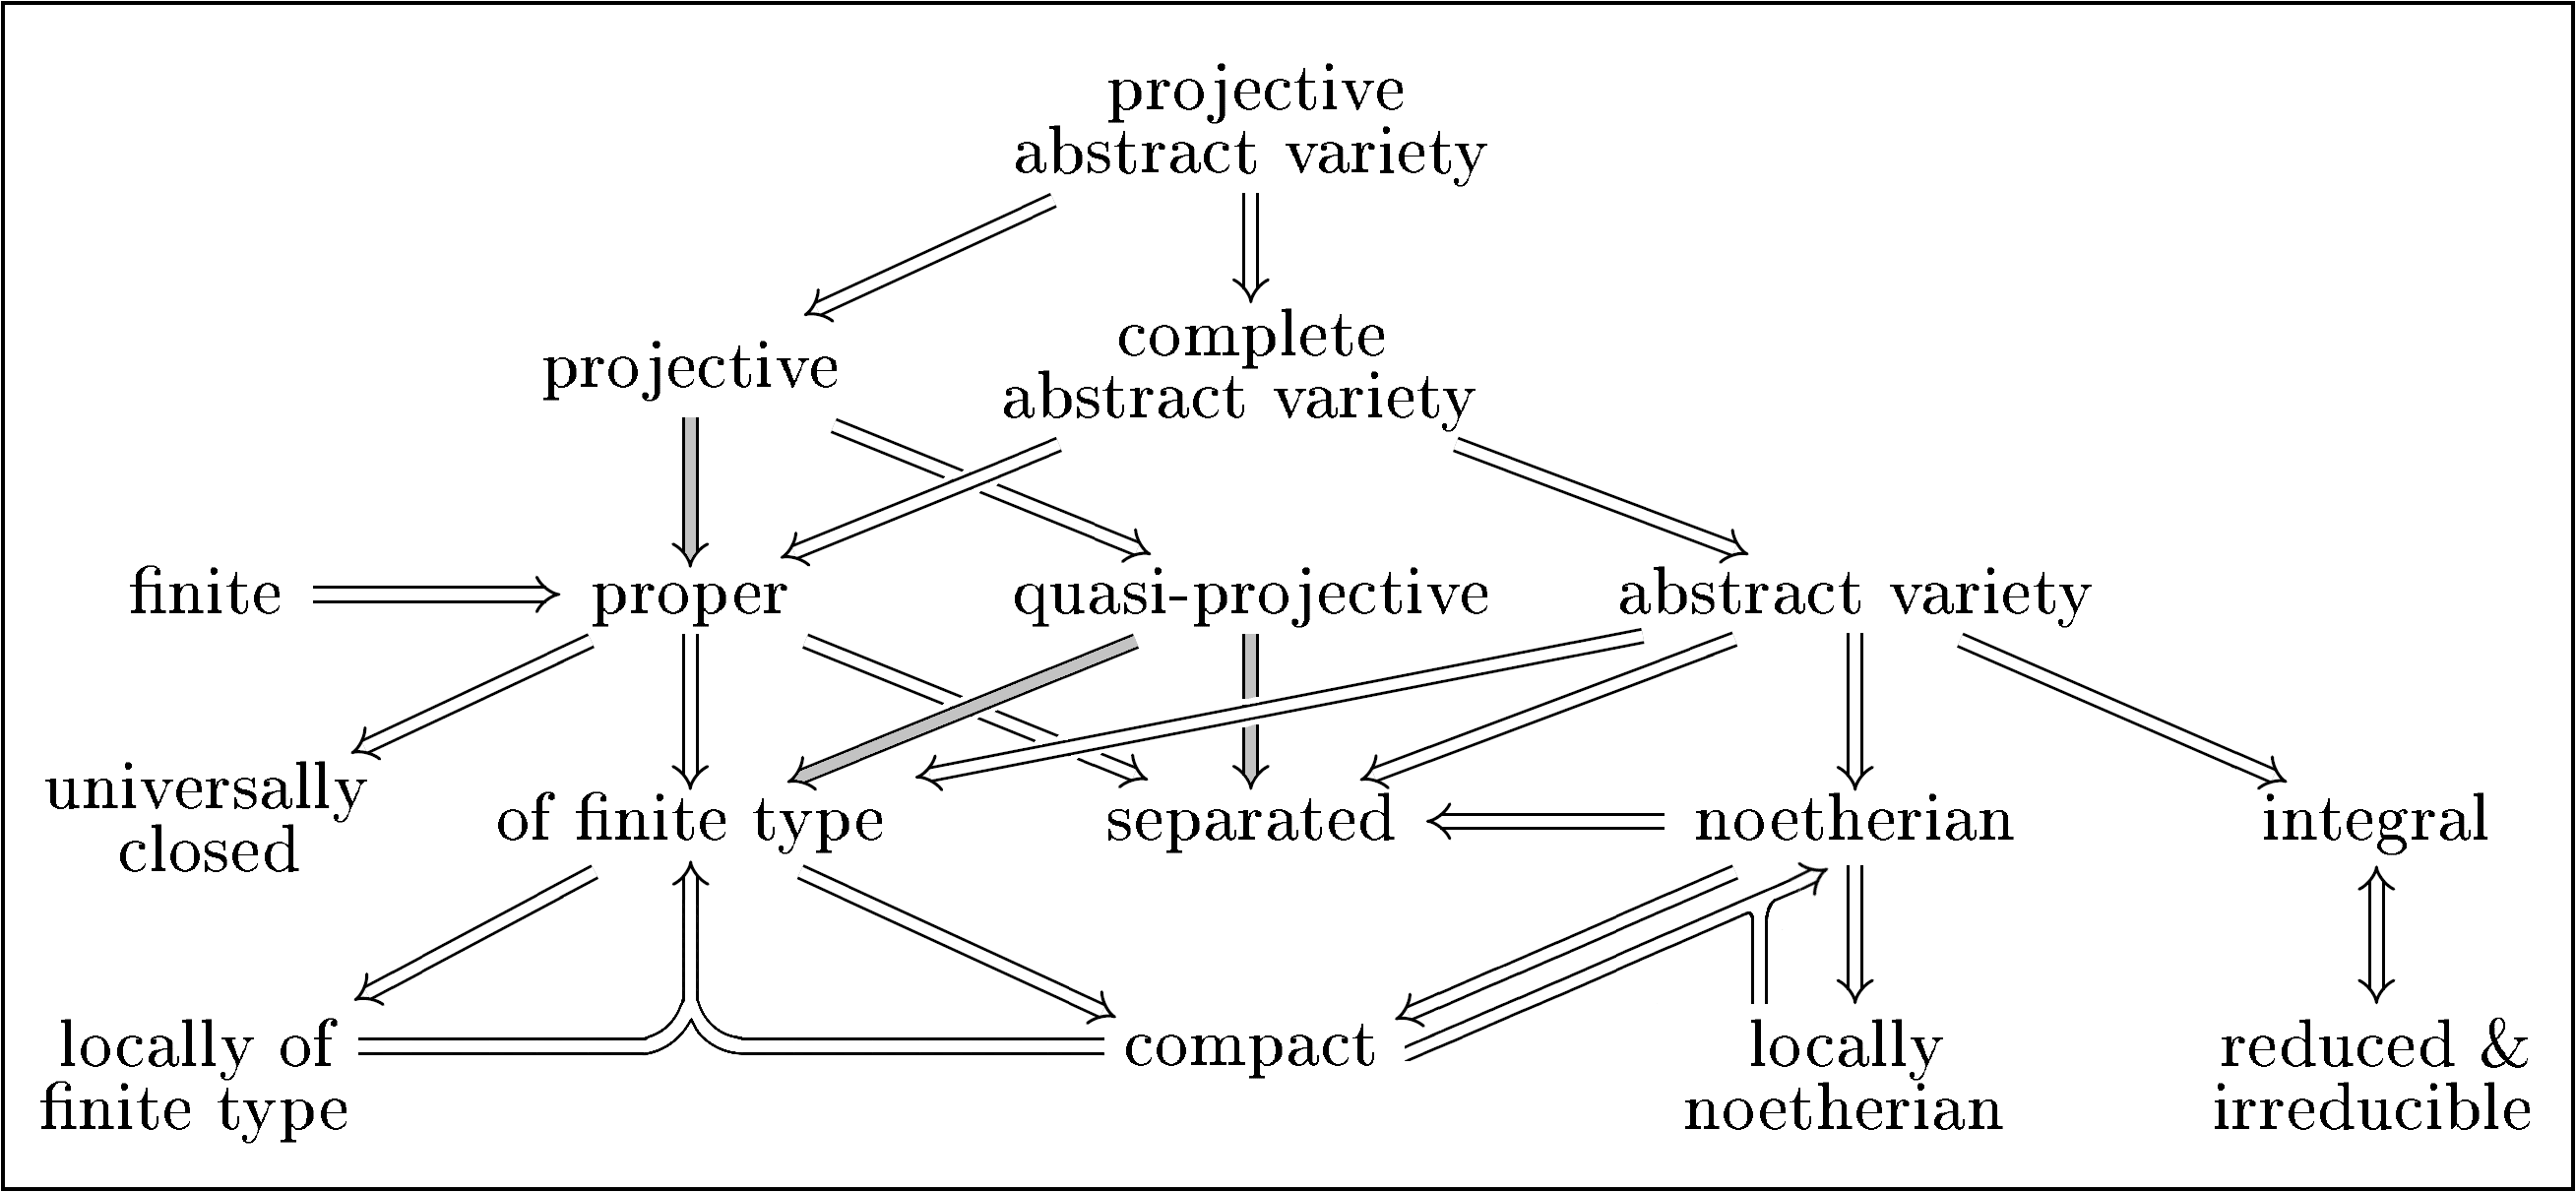
\includegraphics[width=0.95\textwidth]{bigdiagram.png}\quad
\end{figure*}\vspace*{-0.5cm}
% [Tutor Note: 原图位于原 PDF 第 79 页。紧随其后的 equation 环境（标签 bigdiagram）中保留了作者注释掉的 tikzcd 源码，故该方程本身渲染为空；此处按原样保留，便于以后直接编辑该图。]
\begin{equation}\label{bigdiagram}
%\begin{small}
%\begin{tikzpicture}[mybox/.style={draw, inner sep=1.5pt}]
%\node[mybox] (box){
%\begin{tikzcd}[column sep=1em, row sep=0.3cm]
%& & {\begin{aligned}\text{projective}\\[-0.2cm] \text{abstract variety}\end{aligned}}\arrow[dl, Rightarrow]\arrow[d, Rightarrow] & & \\
%& \text{projective}\arrow[d, Rightarrow, crossing over]\arrow[dr, Rightarrow] & {\begin{aligned}\text{complete}\\[-0.2cm] \!\!\text{abstract variety}\end{aligned}}\arrow[dr, Rightarrow]\arrow[dl, Rightarrow] &  & \\
%\text{finite}\arrow[r, Rightarrow] & \text{proper}\arrow[dl, Rightarrow]\arrow[d, crossing over, Rightarrow]\arrow[dr, crossing over, Rightarrow] & {\begin{aligned}\text{quasi-projective}\end{aligned}}\arrow[d, Rightarrow]\arrow[dl, Rightarrow] & {\begin{aligned}\text{abstract variety}\end{aligned}}\arrow[dl, Rightarrow]\arrow[d, Rightarrow]\arrow[dr, Rightarrow]  & \\
%{\begin{aligned}\text{universally}\\[-0.2cm] \!\!\text{closed}\end{aligned}} & {\begin{aligned}\text{of finite type}\end{aligned}}\arrow[dl, Rightarrow]\arrow[dr, Rightarrow]\arrow[urr, Leftarrow] & \text{separated} & \text{noetherian}\arrow[l, Rightarrow]\arrow[d, Rightarrow]\arrow[dl, Rightarrow] & \text{integral}\arrow[d, Leftrightarrow] \\
%{\begin{aligned}\text{locally of}\\[-0.2cm] \!\!\text{finite type}\end{aligned}} &  & \text{compact} & {\begin{aligned}\text{locally}\\[-0.2cm] \!\!\text{noetherian}\end{aligned}}  & {\begin{aligned}\text{reduced \&}\\[-0.2cm] \!\!\text{irreducible}\end{aligned}} 
%\end{tikzcd}
%};
%\end{tikzpicture}\end{small}
\end{equation}

最后，为后文之需，我们希望在仿射概形上的模与模层之间建立一个函子。为此，我们首先需要细化注 \ref{spectra} 中谱的结构层的构造。

\begin{Def}\label{asssheafofmodules}
设 $R$ 是环，$M$ 是（左）$R$-模，$X=\text{Spec}(R)$ 是带有结构层 $\mathcal{O}_X$ 的仿射概形。则\textbf{在 $X$ 上联系于 $M$ 的层 $\widetilde{M}$}\index{sheaf!associated to a module}由下述指定确定：
\begin{small}\begin{align*}
		\widetilde{M}(U)\!\coloneqq\!\bigg\{s\!:U\!\rightarrow\!\bigsqcup_{\mathfrak{p}\in U}\! M_\mathfrak{p}\Bigm|\, &\forall\mathfrak{p}\!\in\! U\!: s(\mathfrak{p})\!\in\! M_\mathfrak{p}\text{ and }\exists U_\mathfrak{p}\!\subset\! U\text{ $\mathfrak{p}$-neighb. }\exists m\!\in\! M\,\exists f\!\in\! R \\[-0.3cm]
		&\text{s.t. }\!\forall\mathfrak{q}\!\in\! U_\mathfrak{p}\text{ holds }f\!\notin\!\mathfrak{q} \text{ and }
		s(\mathfrak{q})\!=\! \frac{m}{f}\!\in\! M_\mathfrak{q}\bigg\}\,,
\end{align*}\end{small}
\!\!对每个开集 $U\subset X$（此处的 $M_\mathfrak{p}$ 表示 $M$ 在素理想 $\mathfrak{p}$ 处的局部化），限制映射按显然方式给出。与谱的结构层类似，可以证明确实有 $\widetilde{M}\in\text{obj}(\mathsf{Sh}(X;{}_{\mathcal{O}_X}\!\mathsf{Mod}))$。
\end{Def}

\begin{Pro}\label{squaretildefunc}
设 $R$ 是环，$M$ 是左 $R$-模，$X=\textup{Spec}(R)$ 是带有结构层 $\mathcal{O}_X$ 的仿射概形。则 $\Gamma(X,\widetilde{M})=M$，并且映射 $M\mapsto\widetilde{M}$ 确定了一个正合、全忠实的函子 $\widetilde{\square}: {}_R\mathsf{Mod}\rightarrow \mathsf{Sh}(X;{}_{\mathcal{O}_X}\!\mathsf{Mod})$。
\end{Pro}

\begin{proof}
等式 $\Gamma(X,\widetilde{M})=M$ 由对 $\Gamma(X,\mathcal{O}_X)\cong R$ 的证明稍作改编得到。其次，$\widetilde{\square}$ 是正合的，因为 $(\widetilde{M})_\mathfrak{p}\cong M_\mathfrak{p}$，而层序列的正合性可在茎的层面检验（由引理 \ref{aboutmonepisheaves}）。最后，对任意 $M, N\in\text{obj}({}_R\mathsf{Mod})$ 都有自然映射 $(\widetilde{\square})_{M,N}:\text{Hom}_R(M,N)\rightarrow\text{Hom}_{\mathcal{O}_X}(\widetilde{M},\widetilde{N})$，按我们最初的论证，其逆为 $\Gamma(X,\square)$，这就证明了它是双射，从而证明了 $\widetilde{\square}$ 的全忠实性。  
\end{proof}

事实上，还可以进一步证明 $\widetilde{\square}$ 与 $\Gamma(X,\square)$ 构成一对伴随函子：对任意 $M\in\text{obj}({}_R\mathsf{Mod})$ 与 $\mathcal{F}\in\text{obj}(\mathsf{Sh}(X;{}_{\mathcal{O}_X}\!\mathsf{Mod}))$ 有 $\text{Hom}_R(M,\Gamma(X,\mathcal{F}))\cong\text{Hom}_{\mathcal{O}_X}(\widetilde{M},\mathcal{F})$。

\begin{Rem}\label{asssheafofmodforproj}
给定分次环 $S$，可以按与定义 \ref{asssheafofmodules} 在仿射概形上的做法类似的方式，在射影谱 $X=\text{Proj}(S)$ 上对任何分次 $S$-模 $M$ 定义联系于它的层 $\widetilde{M}$。结果有 $\widetilde{M}\in\text{obj}(\mathsf{QCoh}(X;{}_{\mathcal{O}_X}\!\mathsf{Mod}))$；并且当 $S$ 诺特且 $M$ 有限生成时，还有 $\widetilde{M}\in\text{obj}(\mathsf{Coh}(X;{}_{\mathcal{O}_X}\!\mathsf{Mod}))$（由 \cite[命题 II.5.11]{[Har77]}）。

于是对任意 $n\in\mathbb{Z}$ 我们令 $\mathcal{O}_X(n)\coloneqq\widetilde{S(n)}\in\text{obj}(\mathsf{QCoh}(X;{}_{\mathcal{O}_X}\!\mathsf{Mod}))$，其中 $S(n)\coloneqq\bigoplus_{k\in\mathbb{Z}}S_{n+k}$。特别地，我们把 $\mathcal{O}_X(1)$ 称为\textit{Serre 扭层}，并把 $\mathcal{F}(n)\coloneqq\mathcal{F}\otimes_{\mathcal{O}_X}\mathcal{O}_X(n)$ 称为 $\mathcal{F}\in\text{obj}(\mathsf{Sh}(X;{}_{\mathcal{O}_X}\!\mathsf{Mod}))$ 的\textit{第 $n$ 次扭层}。

还可以通过 $\Gamma_*(\mathcal{F})\coloneqq\bigoplus_{n\in\mathbb{Z}}\Gamma(X,\mathcal{F}(n))$ 定义\textit{联系于 $\mathcal{F}$ 的分次 $S$-模}，并证明在温和的条件下它诱导出的层同构于 $\mathcal{F}$ 本身（参看 \cite[命题 II.5.15]{[Har77]}）。  
% [Tutor Note: 注意 $\mathcal{O}_X(n)$ 的记号依赖于 $\widetilde{}$ 构造对分次模的平移，即 $S(n)_{d}=S_{n+d}$；而 $\Gamma_*(\mathcal{F})$ 到 $\mathcal{F}$ 的自然映射一般不是同构，原文所谓「温和的条件」指 $S$ 由 $S_1$ 有限生成、$\mathcal{F}$ 拟凝聚等情形（详见 \cite{[Har77]} 第 II.5 节）。]
\end{Rem}

\subsection{拟凝聚层与凝聚层}\label{ch5.6}


在对概形有了更牢固的掌握之后，我们准备从第 \ref{ch5.4} 节中断之处重新拾起层论，首先给出拟凝聚层/凝聚层的另一种定义。

\begin{Rem}\label{disclaimer}(\textit{免责声明})
本节（以及余下理论的相当一部分）严重依赖概形，把由此产生的、难免更为技术性的证明推给文献，并且常常「凭信念」接受某些陈述。不过，读者可以这样自我安慰：只要知道/回想起，\cite{[Imp21]} 中 Floer 理论所提出的那些更偏分析的方面同样受到过一些重大妥协——由于时空限制与作者的无知；与此构成镜像的是，我们眼下略去的这套机制本质上是代数的——这又是镜像对称的另一种体现……总之，我们主要遵循 \cite{[Har77]}，但例如在 \cite[第 13 章]{[Vak17]} 中也能找到丰富的材料。 
\end{Rem}

\begin{Def}\label{quasi-/coherentmodules}
设 $(X,\mathcal{O}_X)$ 是概形。则 $\mathcal{F}\in\text{obj}(\mathsf{Sh}(X;{}_{\mathcal{O}_X}\!\mathsf{Mod}))$ 称为\textbf{拟凝聚 $\mathcal{O}_X$-模}\index{ox@$\mathcal{O}_X$-module!quasi-coherent}，如果 $X$ 可被一族开仿射子集 $U_i=\text{Spec}(R_i)\subset X$ 覆盖，使得对每个 $i$ 都存在 $R_i$-模 $M_i\in\text{obj}({}_{R_i}\!\mathsf{Mod})$，使 $\mathcal{F}|_{U_i}\cong\widetilde{M}_i\in\text{obj}(\mathsf{Sh}(U_i;{}_{\mathcal{O}_{U_i}}\!\mathsf{Mod}))$，其中 $\widetilde{M}_i$ 是按定义 \ref{asssheafofmodules} 联系于 $M_i$ 的层。

若每个 $M_i$ 都可选为有限生成的（从而属于 ${}_{R_i}\!\mathsf{Mod}^\mathsf{fg}\subset {}_{R_i}\!\mathsf{Mod}$），则 $\mathcal{F}$ 进一步称为\textbf{凝聚 $\mathcal{O}_X$-模}\index{ox@$\mathcal{O}_X$-module!coherent}。 

拟凝聚层/凝聚层的态射就是其底层 $\mathcal{O}_X$-模层面的态射。  
\end{Def}

我们强调，由此得到的范畴 $\mathsf{QCoh}(X;{}_{\mathcal{O}_X}\!\mathsf{Mod})$ 与 $\mathsf{Coh}(X;{}_{\mathcal{O}_X}\!\mathsf{Mod})$ 与一般环空间上的对应范畴一致——只要把定义 \ref{coherentonringed} 瞄准概形，更确切地说，在凝聚的情形瞄准诺特概形\footnote{在任意的非诺特概形上，凝聚性表现很坏。}（见 \cite[习题 II.5.4]{[Har77]}）。 

例如，任何概形 $(X,\mathcal{O}_X)$ 的结构层 $\mathcal{O}_X$ 都是凝聚 $\mathcal{O}_X$-模。
% [Tutor Note: 严格地说，「任意概形的结构层 $\mathcal{O}_X$ 都是凝聚 $\mathcal{O}_X$-模」需要（局部）凝聚性假设：在仿射情形 $X=\text{Spec}(R)$，这等价于环 $R$ 是凝聚环，并非对一切环成立。后文命题 \ref{squaretildefunctocoherent} 也只在 $R$ 诺特时给出 $\mathsf{Coh}$ 的等价，可与此对照。]

\begin{Pro}\label{squaretildefunctocoherent}
设 $R$ 是环，$X=\textup{Spec}(R)$ 是带有结构层 $\mathcal{O}_X$ 的仿射概形。则命题 \ref{squaretildefunc} 中的函子 $\widetilde{\square}:M\mapsto\widetilde{M}$ 可以改进为两个等价
\begin{equation}\label{squaretildeequivalences}
	\mkern-18mu\widetilde{\square}:{}_R\mathsf{Mod}\rightarrow\mathsf{QCoh}(X;{}_{\mathcal{O}_X}\!\mathsf{Mod})\quad\text{resp.}\quad \widetilde{\square}:{}_R\mathsf{Mod}^\mathsf{fg}\rightarrow\mathsf{Coh}(X;{}_{\mathcal{O}_X}\!\mathsf{Mod})
\end{equation}
\textup(后者在 $R$ 诺特时成立\textup)，\footnote{且不说 $\mathsf{Coh}(X;{}_{\mathcal{O}_X}\!\mathsf{Mod})$ 表现不良，当 $R$ 非诺特时我们还有 ${}_R\mathsf{Mod}^\mathsf{fg}$ \textit{不是}阿贝尔范畴——这确实相当不理想！} 二者的拟逆均为 $\Gamma(X,\square):\mathcal{F}\mapsto\Gamma(X,\mathcal{F})$。
\end{Pro}  

\begin{proof}
该陈述是下述更一般事实的推论（见 \cite[命题 II.5.4]{[Har77]}）：对一般概形 $(X,\mathcal{O}_X)$，$\mathcal{F}\in\text{obj}(\mathsf{Sh}(X;{}_{\mathcal{O}_X}\!\mathsf{Mod}))$ 是拟凝聚的，当且仅当对每个开集 $U=\text{Spec}(R_U)\subset X$ 都存在某个 $M\in\text{obj}({}_{R_U}\!\mathsf{Mod})$ 使 $\mathcal{F}|_U\cong\widetilde{M}\in\text{obj}(\mathsf{Sh}(U;{}_{\mathcal{O}_U}\!\mathsf{Mod}))$；而它在 $X$ 诺特时是凝聚的，当且仅当此外还有 $M\in\text{obj}({}_{R_U}\!\mathsf{Mod}^\mathsf{fg})$。（其实，这些只是定义 \ref{quasi-/coherentmodules} 的等价改写。）

在上式中取 $U=X$，即 $R_U=R$，就得到 $\widetilde{\square}$ 的本质满性；而 $\mathcal{O}_X$-模态射层面的全忠实性由命题 \ref{squaretildefunc} 提供（回忆：函子是等价当且仅当它全忠实且本质满）。后者同时确认 $\Gamma(X,\square)$ 是对应的拟逆。  
\end{proof}

\begin{Pro}\label{cokernelscoherent}
设 $X$ 是概形。任何拟凝聚层态射的核层、余核层与像层本身都是拟凝聚的。 

若 $X$ 还是诺特的，则任何凝聚层态射的核、余核与像也都是凝聚的。
\end{Pro}

\begin{proof}
这是局部验证，故不妨取 $X=\text{Spec}(R)$ 为仿射的。但此时 \eqref{squaretildeequivalences} 使我们能把任何拟凝聚层/凝聚层的态射视为模（分别地，有限生成模）的态射。${}_R\mathsf{Mod}$ 与 ${}_R\mathsf{Mod}^\mathsf{fg}$ 都是阿贝尔范畴（后者需 $R$ 诺特），故它们包含其任意态射的核、余核与像。再用等价 $\widetilde{\square}$ 即得命题。  
\end{proof}

作为直接推论，我们得到本节的基本结果，它使凝聚层的导出范畴之存在合法化。

\begin{Cor}\label{QCohisabelian}
对任何概形 $(X,\mathcal{O}_X)$，范畴 $\mathsf{QCoh}(X;{}_{\mathcal{O}_X}\!\mathsf{Mod})$ 都是阿贝尔范畴；而对任何诺特概形 $(X,\mathcal{O}_X)$，范畴 $\mathsf{Coh}(X;{}_{\mathcal{O}_X}\!\mathsf{Mod})$ 都是阿贝尔范畴。
\end{Cor}

\begin{proof}
由于 $\mathsf{QCoh}(X;{}_{\mathcal{O}_X}\!\mathsf{Mod})$ 与 $\mathsf{Coh}(X;{}_{\mathcal{O}_X}\!\mathsf{Mod})$ 都是阿贝尔范畴 $\mathsf{Sh}(X;{}_{\mathcal{O}_X}\!\mathsf{Mod})$ 的全子范畴，只需验证它们对有限直和与余核/核封闭。后者由命题 \ref{cokernelscoherent} 提供；至于前者，我们注意到：给定两个拟凝聚层/凝聚层 $\mathcal{F}, \mathcal{G}$ 以及它们共同的开覆盖 $\{U_i\}_{i\in I}$，局部地有 $(\mathcal{F}\oplus\mathcal{G})|_{U_i}=\mathcal{F}|_{U_i}\oplus\mathcal{G}|_{U_i}\cong \widetilde{M}_i\oplus\widetilde{N}_i\cong(\widetilde{M\oplus N})_i$（对合适的模），从而 $\mathcal{F}\oplus\mathcal{G}$ 也是拟凝聚的/凝聚的。最后，零层显然是拟凝聚的/凝聚的。
% [Tutor Note: 这里用到的判据是：阿贝尔范畴的全子范畴若对有限直和（从而含零对象）以及核、余核封闭，则它自身是阿贝尔范畴，且包含函子是正合的。末句「零层显然拟凝聚」正是补上零对象这一条。]
\end{proof}

\begin{Rem}\label{desirablecoherentprop}
让我们强调哪些良好的性质在拟凝聚性/凝聚性下得以保持。设 $(X,\mathcal{O}_X)$ 是概形。
\begin{itemize}[leftmargin=0.5cm]
	\item 给定拟凝聚层 $\mathcal{F}$，Hom 群与局部 $\mathcal{H}om$-层给出
	\begin{equation}\label{locHomonqcoh}
		\begin{aligned}
			&\text{Hom}_{\mathcal{O}_X}\!(\mathcal{F},\square):\mathsf{QCoh}(X;{}_{\mathcal{O}_X}\!\mathsf{Mod})\rightarrow \mathsf{Ab}\,, \\
			&\mathcal{H}om_{\mathcal{O}_X}\!(\mathcal{F},\square):\mathsf{QCoh}(X;{}_{\mathcal{O}_X}\!\mathsf{Mod})\rightarrow \mathsf{QCoh}(X;{}_{\mathcal{O}_X}\!\mathsf{Mod})\,, 
		\end{aligned}
	\end{equation}
	二者都是左正合的。若 $\mathcal{F}$ 还是凝聚层，则这些函子特化为左正合的
	\begin{equation}\label{locHomoncoh}
		\begin{aligned}
			&\text{Hom}_{\mathcal{O}_X}\!(\mathcal{F},\square):\mathsf{Coh}(X;{}_{\mathcal{O}_X}\!\mathsf{Mod})\rightarrow \mathsf{Vect}_\mathbb{K}\,, \\
			&\mathcal{H}om_{\mathcal{O}_X}\!(\mathcal{F},\square):\mathsf{Coh}(X;{}_{\mathcal{O}_X}\!\mathsf{Mod})\rightarrow \mathsf{Coh}(X;{}_{\mathcal{O}_X}\!\mathsf{Mod})
		\end{aligned}
	\end{equation}
	（其中对 Hom 我们还进一步假定了 $X\in\text{obj}(\mathsf{Sch}(\mathbb{K}))$ 是射影的，并用 $\mathsf{Vect}_\mathbb{K}$ 记 $\mathbb{K}$ 上有限维向量空间的范畴）。
	\newline 类似地，我们有反变左正合函子 $\text{Hom}_{\mathcal{O}_X}\!(\square,\mathcal{F})$ 与 $\mathcal{H}om_{\mathcal{O}_X}\!(\square,\mathcal{F})$。特别地，凝聚层 $\mathcal{F}$ 的对偶层 $\mathcal{F}^\vee=\mathcal{H}om_{\mathcal{O}_X}\!(\mathcal{F},\mathcal{O}_X)$ 也是凝聚的。
	
	\item 张量运算对拟凝聚层/凝聚层同样表现良好，给出右正合函子 \begin{equation}\label{tensoronqcoh}
		\begin{aligned}
			&\mathcal{F}\otimes_{\mathcal{O}_X}\!\square:\mathsf{QCoh}(X;{}_{\mathcal{O}_X}\!\mathsf{Mod})\rightarrow \mathsf{QCoh}(X;{}_{\mathcal{O}_X}\!\mathsf{Mod})\,, \\
			&\square\!\otimes_{\mathcal{O}_X}\mathcal{G}:\mathsf{QCoh}(X;\mathsf{Mod}_{\mathcal{O}_X})\rightarrow \mathsf{QCoh}(X;{}_{\mathcal{O}_X}\!\mathsf{Mod})\,,
		\end{aligned}
	\end{equation}
	其中分别要求 $\mathcal{F}\in\text{obj}(\mathsf{QCoh}(X;\mathsf{Mod}_{\mathcal{O}_X}))$ 与 $\mathcal{G}\in\text{obj}(\mathsf{QCoh}(X;{}_{\mathcal{O}_X}\!\mathsf{Mod}))$；当 $\mathcal{F},\mathcal{G}$ 分别是凝聚的右、左 $\mathcal{O}_X$-模时，则给出右正合的
	\begin{equation}\label{tensoroncoh}
		\begin{aligned}
			&\mathcal{F}\otimes_{\mathcal{O}_X}\!\square:\mathsf{Coh}(X;{}_{\mathcal{O}_X}\!\mathsf{Mod})\rightarrow \mathsf{Coh}(X;{}_{\mathcal{O}_X}\!\mathsf{Mod})\,, \\
			&\square\!\otimes_{\mathcal{O}_X}\mathcal{G}:\mathsf{Coh}(X;\mathsf{Mod}_{\mathcal{O}_X})\rightarrow \mathsf{Coh}(X;{}_{\mathcal{O}_X}\!\mathsf{Mod})\,,
		\end{aligned}
	\end{equation}。
	\newline 注意在仿射的 $X=\text{Spec}(R)$ 上有 $\Gamma(X,\mathcal{F}\otimes_{\mathcal{O}_X}\!\mathcal{G})\cong\Gamma(X,\mathcal{F})\otimes_R \Gamma(X,\mathcal{G})$。这可用来定义并证明拟凝聚层的张量幂、对称幂与外幂都是拟凝聚的。
	
	\item 给定拟凝聚层的短正合序列 $0\rightarrow\mathcal{F}_1\rightarrow\mathcal{F}_2\rightarrow\mathcal{F}_3\rightarrow 0$，若 $\mathcal{F}_1$ 与 $\mathcal{F}_3$ 也是局部自由的，则 $\mathcal{F}_2$ 也必局部自由（在仿射子集上，对自由层有同样的结论）。
	\newline 再假设 $X$ 是诺特的，并设 $\mathcal{F}$ 是凝聚 $\mathcal{O}_X$-模。则 $\mathcal{F}$ 局部自由当且仅当对每个 $x\in X$，$\mathcal{F}_x$ 是自由 $\mathcal{O}_{X,x}$-模；而它是可逆层当且仅当存在另一个凝聚层 $\mathcal{G}$ 使 $\mathcal{F}\otimes_{\mathcal{O}_X}\!\mathcal{G}\cong\mathcal{O}_X$。 
\end{itemize}
% [Tutor Note: 上一条中原文混用了 $\mathsf{QCoh}(X;\mathsf{Mod}_{\mathcal{O}_X})$ 与 $\mathsf{QCoh}(X;{}_{\mathcal{O}_X}\!\mathsf{Mod})$ 两种写法，二者指同一个范畴（左 $\mathcal{O}_X$-模层）；张量积两端的模结构（右、左）也须与之匹配，此处照原文保留。]
\end{Rem}

特别有用的是弄清拉回与推前函子如何与拟凝聚层/凝聚层相互作用。回顾上一节的众多定义，我们有：

\begin{Pro}\label{pushpullcoherent}
设 $f:(X,\mathcal{O}_X)\rightarrow (Y,\mathcal{O}_Y)$ 是概形态射 \textup(从而是底层局部环空间的态射；参看定义 \ref{locallyringedspace}\textup)。则：
\renewcommand{\theenumi}{\roman{enumi}}
\begin{enumerate}[leftmargin=0.6cm]
	\item 拉回函子特化为 $f^*\!\!: \mathsf{QCoh}(Y;{}_{\mathcal{O}_Y}\!\mathsf{Mod})\!\rightarrow\!\mathsf{QCoh}(X;{}_{\mathcal{O}_X}\!\mathsf{Mod})$，并且当 $X$、$Y$ 都诺特时，特化为 $f^*\!: \mathsf{Coh}(Y;{}_{\mathcal{O}_Y}\!\mathsf{Mod})\rightarrow \mathsf{Coh}(X;{}_{\mathcal{O}_X}\!\mathsf{Mod})$。二者都是右正合的。
	
	\item 若 $X$ 诺特，或 $f$ 分离且紧，则推前函子特化为左正合的 $f_*\!: \mathsf{QCoh}(X;{}_{\mathcal{O}_X}\!\mathsf{Mod})\!\rightarrow \!\mathsf{QCoh}(Y;{}_{\mathcal{O}_Y}\!\mathsf{Mod})$。 
	\newline 此外，若 $f$ 是诺特概形之间的有限态射，或是域 $\mathbb{K}$ 上有限型概形之间的射影态射——更一般地，若 $f$ 是诺特概形之间的固有态射——则它诱导左正合的 $f_*: \mathsf{Coh}(X;{}_{\mathcal{O}_X}\!\mathsf{Mod})\rightarrow \mathsf{Coh}(Y;{}_{\mathcal{O}_Y}\!\mathsf{Mod})$。  
\end{enumerate}
\end{Pro}

\begin{proof}(\textit{概要})
关于拉回，问题是局部的，故可设 $X$ 与 $Y$ 都是仿射的。于是应用命题 \ref{squaretildefunctocoherent} 以及 \cite[命题 II.5.2]{[Har77]} 即得第 \textit{i} 点。注意 $f^*=\mathcal{O}_X\otimes_{f^{\!-\!1}\!\mathcal{O}_Y}\! f^{-1}(\square)$ 的右正合性继承自 $f^{-1}$ 与张量积的右正合性。 

关于推前，按假设可取 $Y$ 为仿射的，并用有限多个开仿射子集覆盖 $X$（因为 $f$ 是紧的）。于是为证明对任意 $\mathcal{F}\in\text{obj}(\mathsf{QCoh}(X;{}_{\mathcal{O}_X}\!\mathsf{Mod}))$ 有 $f_*\mathcal{F}\in\text{obj}(\mathsf{QCoh}(Y;{}_{\mathcal{O}_Y}\!\mathsf{Mod}))$，只需利用：任意一对拟凝聚层 $\mathcal{G}_1,\mathcal{G}_3$ 的扩充 $\mathcal{G}_2$——按定义，它装入短正合序列 $0\rightarrow\mathcal{G}_1\rightarrow\mathcal{G}_2\rightarrow\mathcal{G}_3\rightarrow 0$——本身也是拟凝聚的（见 \cite[命题 II.5.7]{[Har77]}）。 

把 $f_*$ 限制到凝聚层上，我们只说明 $f$ 为射影的情形如何证明：由局部性，取 $Y=\text{Spec}(A)$，其中 $A$ 是有限生成的 $\mathbb{K}$-代数（从而是环），于是对任意 $\mathcal{F}\in\text{obj}(\mathsf{Coh}(X;{}_{\mathcal{O}_X}\!\mathsf{Mod}))$，前一点已保证 $f_*\mathcal{F}$ 是拟凝聚的；再由命题 \ref{squaretildefunctocoherent} 有 $f_*\mathcal{F}\cong(\widetilde{\square}\circ\Gamma(Y,\square))(f_*\mathcal{F})=\widetilde{\square}\big(\mathcal{F}(f^{-1}(Y))\big)=\Gamma(X,\mathcal{F})^\sim$，而它实际上是凝聚的，因为 $\Gamma(X,\mathcal{F})$ 是有限生成的 $A$-模（由 \cite[定理 II.5.19]{[Har77]}）。$f$ 固有时的更一般证明见 \cite[第 III.8 节]{[Har77]}。  
\end{proof}
% [Tutor Note: 值得强调 $f_*$ 一般\emph{并不}保持拟凝聚性：原文给出的两个充分条件（$X$ 诺特，或 $f$ 分离且紧）都不可省；完整证明被推给 \cite{[Har77]} 第 II.5 节与第 III.8 节。另外 $f^*$ 的右正合性与 $f_*$ 的左正合性，也可由它们构成伴随对（同构 \eqref{pullpushareadjoints}）直接读出。]

注意 $f^*$ 与 $f_*$ 的右、左正合性同样可由它们构成一对伴随函子推出（见同构 \eqref{pullpushareadjoints}），即使在拟凝聚/凝聚的世界里也是如此。

\begin{Cor}\label{globalsectforcoherent}
设 $X$ 是诺特概形。则引理 \ref{sectfuncexact} 的整体截面函子 \textup(取 $U=X$ 时\textup)特化为左正合函子：
\begin{equation}
	\begin{aligned}
		&\Gamma(X,\square): \mathsf{QCoh}(X;{}_{\mathcal{O}_X}\!\mathsf{Mod})\rightarrow\mathsf{Ab}\,, \\
		&\Gamma(X,\square):\mathsf{Coh}(X;{}_{\mathcal{O}_X}\!\mathsf{Mod})\rightarrow\mathsf{Ab}\,.
	\end{aligned}
\end{equation}
特别地，若 $X\in\textup{obj}(\mathsf{Sch}(\mathbb{K}))$ 是 $\mathbb{K}$ 上的诺特概形，分别地是射影的\textup(或仅为固有的\textup)概形，则我们有左正合函子：
\begin{equation}\label{globsectsfunconcoh}
	\begin{aligned}
		&\Gamma(X,\square):\mathsf{QCoh}(X;{}_{\mathcal{O}_X}\!\mathsf{Mod})\rightarrow\mathsf{Vect}_\mathbb{K}^{\leq\infty}\,, \\
		&\Gamma(X,\square):\mathsf{Coh}(X;{}_{\mathcal{O}_X}\!\mathsf{Mod})\rightarrow\mathsf{Vect}_\mathbb{K}
	\end{aligned}
\end{equation}
\textup(其中 $\mathsf{Vect}_\mathbb{K}^{\leq\infty}$ 是可能无穷维的 $\mathbb{K}$-向量空间所成的范畴\textup)。 
\end{Cor}

\begin{proof}
这由命题 \ref{pushpullcoherent} 直接得到：只需取\footnote{在下文注 \ref{sectfuncispushforward} 中我们将看到，对模层也有同样的结论，只要把目标空间取为配以合适常层的单点空间。} $Y=\text{Spec}(\mathbb{K})$，并取 $f:X\rightarrow \text{Spec}(\mathbb{K})$ 为结构态射，它在 $\mathbb{K}$ 上是固有的。再由引理 \ref{sectfuncexact} 即得左正合性。 

若 $X$ 在 $\mathbb{K}$ 上射影，则上一个证明已经提示：对任意 $\mathcal{F}\in\text{obj}(\mathsf{Coh}(X;{}_{\mathcal{O}_X}\!\mathsf{Mod}))$，$\Gamma(X,\mathcal{F})$ 是有限生成的 $\mathbb{K}$-模（这一事实在定理 \ref{sheafcohomforprojsch} 的证明中有更一般的说明），即有限维 $\mathbb{K}$-向量空间。放松到拟凝聚层，我们只是允许无限维的向量空间出现。
\end{proof}


\newpage
\pagestyle{fancy}


% 译自 arXiv:2306.13589v2 原 tex 第 2960–3572 行
\section{凝聚层的导出范畴}
\thispagestyle{plain}

\takeaway{%
  \textbf{物理图像：}本节为同调镜像对称的 B-侧搭好舞台：凝聚层的导出范畴在物理上就是 B-模型里 D-膜所构成的范畴，而层之间的 $\text{Ext}$ 群给出 D-膜之间的态射空间。\\
  \textbf{数学工具：}环空间上模层的导出范畴（内射消解与右导出函子）、作为张量函子适配类的平坦层、层上同调与 \v{C}ech 上同调及其在诺特分离概形上的比较。\\
  \textbf{主要结论：}模层范畴有足够多的内射对象，故 $\mathsf{R}\Gamma$、$\mathsf{R}f_*$、$\mathsf{R}\mathcal{H}om$ 等右导出函子存在；在诺特分离概形上、对拟凝聚层，\v{C}ech 上同调可用以计算层上同调；在光滑射影簇上，凝聚层有界导出范畴上的这些导出函子满足投影公式、伴随公式、平坦基变换与 Künneth 公式。%
}

\subsection{模层上的导出函子}\label{ch6.1}

让我们暂且退一步，重新把注意力放回模层上；只有在这一基础工作完成之后，我们才会在第 \ref{ch6.2} 节进行到一半时回到概形与凝聚层。

根据定理 \ref{Sh(X,Ab)isabelian}、注 \ref{sheafmodulesrem}a. 以及我们在第 2 章所作的分析，对取值于任意阿贝尔范畴 $\mathsf{A}$ 的、拓扑空间 $X$ 上的层，我们可以合法地谈论其导出范畴 $\mathsf{D}(\mathsf{Sh}(X;\mathsf{A}))$；相应地，对环空间 $(X,\mathcal{S})$ 上的 $\mathcal{S}$-模，也可以谈论其导出范畴 $\mathsf{D}(\mathsf{Sh}(X;{}_\mathcal{S}\mathsf{Mod}))$。我们已经知道若干个联系它们底层层范畴的函子，那么不妨看看它们是否诱导出导出函子。

\begin{Pro}\label{enoughinjectivemodules}
设 $(X,\mathcal{S})$ 为环空间。则 $\mathsf{Sh}(X;{}_\mathcal{S}\mathsf{Mod})$ 有足够多的内射对象 \textup(从而由注 \ref{sheafmodulesrem}b.，对任意阿贝尔范畴 $\mathsf{A}$，$\mathsf{Sh}(X;\mathsf{A})$ 也有足够多的内射对象\textup)。
\end{Pro}

\begin{proof}
根据定义 \ref{injprojobj}，需要证明的是：任意 $\mathcal{F}\in\text{obj}(\mathsf{Sh}(X;{}_\mathcal{S}\mathsf{Mod}))$ 都容许一个由内射 $\mathcal{S}$-模构成的右消解，特别地，$\mathcal{F}$ 单射入某个作为对象为内射的 $\mathcal{I}\in\text{obj}(\mathsf{Sh}(X;{}_\mathcal{S}\mathsf{Mod}))$。

首先注意到，对每个 $x\in X$，茎 $\mathcal{F}_x\in\text{obj}({}_{\mathcal{S}_x}\!\mathsf{Mod})$ 单射入另一个 $\mathcal{S}_x$-模 $I_x$，而后者作为 ${}_{\mathcal{S}_x}\!\mathsf{Mod}\equiv\mathsf{Sh}(\{x\};{}_\mathcal{S}\mathsf{Mod})$ 的对象是内射的\footnote{这是标准代数中的已知事实：给定环 $R$，每个 $R$-模都同构于某个内射 $R$-模的子模。}。记嵌入为 $\iota_x:\{x\}\hookrightarrow X$，于是 $(\iota_x)_*I_x\in\text{obj}(\mathsf{Sh}(X;{}_\mathcal{S}\mathsf{Mod}))$ 就是相应的摩天层（见例 \ref{skyscrapersheaf}）；今考虑层 $\mathcal{I}\coloneqq\prod_{x\in X}(\iota_x)_*I_x$（它是 $\mathcal{S}$-模，因为 $\mathsf{Sh}(X;{}_\mathcal{S}\mathsf{Mod})$ 是阿贝尔范畴，从而包含其对象的积！），其茎满足 $\mathcal{I}_x\cong I_x$。

给定任意另一个 $\mathcal{S}$-模 $\mathcal{G}$，我们有典范同构 $\text{Hom}_\mathcal{S}(\mathcal{G},\mathcal{I})\cong\prod_{x\in X}\text{Hom}_\mathcal{S}(\mathcal{G},(\iota_x)_*I_x)$。反过来，对每个 $x\in X$ 有 $\text{Hom}_\mathcal{S}(\mathcal{G},(\iota_x)_*I_x)\cong\text{Hom}_{\mathcal{S}_x}(\mathcal{G}_x,I_x)$，因为左端任意 $\mathcal{S}$-模态射 $\chi$ 在集合层面要么是到 $I_x$ 的常值映射 $\chi_U\cong\chi_x$（当 $x\in U$ 时），要么是零映射（否则）。取 $\mathcal{G}=\mathcal{F}$，所得的同构 $\text{Hom}_\mathcal{S}(\mathcal{F},\mathcal{I})\cong\prod_{x\in X}\text{Hom}_{\mathcal{S}_x}(\mathcal{F}_x,I_x)$ 告诉我们：局部单射 $\mathcal{F}_x\hookrightarrow I_x$ 诱导出一个 $\mathcal{S}$-模态射 $\mathcal{F}\rightarrow\mathcal{I}$，而它在茎上单射，故自身也是单射。

现在，回顾正合茎函子 $\square_x: \mathsf{Sh}(X;{}_\mathcal{S}\mathsf{Mod})\rightarrow{}_{\mathcal{S}_x}\!\mathsf{Mod}$ 的存在性，我们观察到按构造有
\[
\text{Hom}_\mathcal{S}(\square,\mathcal{I})=\prod_{x\in X}(\text{Hom}_{\mathcal{S}_x}(\square,I_x)\circ\square_x):\mathsf{Sh}(X;{}_\mathcal{S}\mathsf{Mod})^\text{opp}\rightarrow\mathsf{Ab}\,.
\] 
但如引理 \ref{Homforinjprojobj} 所提示的，每个左正合函子 $\text{Hom}_{\mathcal{S}_x}(\square,I_x):{}_{\mathcal{S}_x}\!\mathsf{Mod}^\text{opp}\rightarrow\mathsf{Ab}$ 实际上是正合的！因此，它与 $\square_x$ 的复合也正合，再取直积之后仍然正合。于是 $\text{Hom}_\mathcal{S}(\square,\mathcal{I})$ 正合。最后，再次由引理 \ref{Homforinjprojobj} 推知，$\mathcal{I}$ 必是内射的 $\mathcal{S}$-模层，此即所欲证者。
\end{proof}

因此，由引理 \ref{enoughinjprojobj} 与定义 \ref{derivedfunc}，我们可以考虑从 $\mathsf{Sh}(X;\mathsf{A})$ 或 $\mathsf{Sh}(X;{}_\mathcal{S}\mathsf{Mod})$ 出发的左正合函子的右导出函子：

\begin{Ex}
设 $f:(X,\mathcal{S}_X)\rightarrow (Y,\mathcal{S}_Y)$ 为环空间态射，并给定任意 $\mathcal{F}\in\text{obj}(\mathsf{Sh}(X;\mathsf{A}))$ 与 $\mathcal{G}\in\text{obj}(\mathsf{Sh}(X;{}_{\mathcal{S}_X}\!\mathsf{Mod}))$，则最突出的右导出函子的例子如下：
\begin{itemize}[leftmargin=0.5cm]
	\item (由例 \ref{exactfuncexample})
	\begin{equation}
		\begin{aligned}
			&\mathsf{R}\text{Hom}_{\mathsf{Sh}(X;\mathsf{A})}(\mathcal{F},\square):\mathsf{D^+}(\mathsf{Sh}(X;\mathsf{A}))\rightarrow\mathsf{D^+(Ab)}\,, \\ 
			&\mathsf{R}\text{Hom}_{\mathcal{S}_X}(\mathcal{G},\square):\mathsf{D^+}(\mathsf{Sh}(X;{}_{\mathcal{S}_X}\!\mathsf{Mod}))\rightarrow\mathsf{D^+(Ab)}\,. \\
		\end{aligned}
	\end{equation}
	
	\item (由定义 \ref{moresheafofmodules})
	\begin{equation}\label{localExtfunc}\begin{footnotesize}
			\mkern-12mu\mathcal{E}xt_{\mathcal{S}_X}\!(\mathcal{G},\square)\!\coloneqq\!\mathsf{R}\mathcal{H}om_{\mathcal{S}_X}\!(\mathcal{G},\square)\!:\!\mathsf{D^+}(\mathsf{Sh}(X;{}_{\mathcal{S}_X}\!\mathsf{Mod}))\!\rightarrow\!\mathsf{D^+}(\mathsf{Sh}(X;{}_{\mathcal{S}_X}\!\mathsf{Mod})), \\
		\end{footnotesize}
	\end{equation}
	类似地还可定义阿贝尔群层上的版本。（关于 $\mathcal{E}xt$ 的更多内容见下文定义 \ref{localExt}。）
	
	\item (由引理 \ref{inversepushforwardexact})
	\begin{equation}
		\begin{aligned}
			&\mathsf{R}f_*:\mathsf{D^+}(\mathsf{Sh}(X;\mathsf{A}))\rightarrow\mathsf{D^+}(\mathsf{Sh}(Y;\mathsf{A}))\,, \\ &\mathsf{R}f^{-1}:\mathsf{D^+}(\mathsf{Sh}(Y;\mathsf{A}))\rightarrow\mathsf{D^+}(\mathsf{Sh}(X;\mathsf{A}))\,.
		\end{aligned}
	\end{equation}
	
	\item (由推论 \ref{pullbackpushforwardexact})
	\begin{equation}\label{Rflowerstar}
		\mathsf{R}f_*:\mathsf{D^+}(\mathsf{Sh}(X;{}_{\mathcal{S}_X}\!\mathsf{Mod}))\rightarrow\mathsf{D^+}(\mathsf{Sh}(Y;{}_{\mathcal{S}_Y}\!\mathsf{Mod}))
	\end{equation} 
	
	\item (由引理 \ref{sectfuncexact}，对任意开集 $U\subset X$) 
	\begin{equation}\label{RGammaU}
		\mathsf{R}\Gamma(U,\square):\mathsf{D^+}(\mathsf{Sh}(X;\mathsf{A}))\rightarrow\mathsf{D^+(A)}\,.
	\end{equation}	  
\end{itemize}\vspace*{-0.2cm}
\hfill $\blacklozenge$ 
\end{Ex}

% [Tutor Note: 此处右导出函子存在的依据是命题 \ref{enoughinjectivemodules}：$\mathsf{Sh}(X;\mathsf{A})$ 有足够多的内射对象。注意这里 $U\subset X$ 不必是仿射的，$\mathsf{R}\Gamma(U,\square)$ 也只是左正合函子 $\Gamma(U,\square)$ 的右导出；若 $U$ 仿射而 $X$ 是分离概形，则由本节关于 \v{C}ech 上同调计算层上同调的定理可知它在高阶为零。]
\begin{Rem}\label{sectfuncispushforward}
以下几件事值得考虑，先给出一点警告。
\begin{itemize}[leftmargin=0.5cm]
	\item (重要警告) 我们\textit{不能}用同样的方法构造左正合函子 $\text{Hom}_{\mathsf{Sh}(X;\mathsf{A})}(\square,\mathcal{F})$、$\text{Hom}_{\mathcal{S}_X}(\square,\mathcal{G})$ 与 $\mathcal{H}om_{\mathcal{S}_X}\!(\square,\mathcal{G})$ 的右导出函子，因为这些是反变函子，也就是说我们要求源范畴有足够多的投射对象而非内射对象。然而这一点并不成立，我们稍后在考察左导出函子是否存在时会提到。
	
	\item 考虑上述右导出 Hom 函子的经典导出函子（见定义 \ref{classicalderivedfunc}），由命题 \ref{ExtRHom} 我们得到 \eqref{Extmodules} 处提到的层论 Ext 函子的另一种刻画（这一般被当作它们的默认定义）：
	\begin{equation}\label{ExtRHomformodules}
		\begin{aligned}
			&\text{Ext}_{\mathsf{Sh}(X;\mathsf{A})}^n(\mathcal{F},\square)\cong\mathsf{R}^n\text{Hom}_{\mathsf{Sh}(X;\mathsf{A})}(\mathcal{F},\square):\mathsf{Sh}(X;\mathsf{A})\rightarrow\mathsf{Ab}\,, \\ 
			&\text{Ext}_{\mathcal{S}_X}^n(\mathcal{G},\square)\cong\mathsf{R}^n\text{Hom}_{\mathcal{S}_X}(\mathcal{G},\square):\mathsf{Sh}(X;{}_{\mathcal{S}_X}\!\mathsf{Mod})\rightarrow\mathsf{Ab}\,, \\ 
		\end{aligned}  
	\end{equation}
	对每个 $n\in\mathbb{N}$ 成立（借助定理 \ref{Extprop}，我们知道当 $n<0$ 时这些是平凡函子，而当 $n=0$ 时则恢复原本的 Hom 函子）。
	
	\item 函子 \eqref{Rflowerstar} 对每个 $n\in\mathbb{Z}$ 诱导出经典的 $\mathsf{R}^nf_*:\mathsf{Sh}(X;{}_{\mathcal{S}_X}\!\mathsf{Mod})\rightarrow\mathsf{Sh}(Y;{}_{\mathcal{S}_Y}\!\mathsf{Mod})$。人们称它们为\textit{高阶直接像函子}；并且对任意 $\mathcal{S}_X$-模 $\mathcal{F}$，称 $\mathsf{R}^nf_*(\mathcal{F})=H^n(\mathsf{R}f_*(\mathcal{F}))\in\text{obj}(\mathsf{Sh}(Y;{}_{\mathcal{S}_Y}\!\mathsf{Mod}))$ 为 $\mathcal{F}$ 的\textbf{高阶直接像}\index{higher direct image}。
	
	\item 特别地取 $(Y,\mathcal{S}_Y)=(\{y\},\underline{\mathbb{Z}})$，所得的推前函子 $f_*:\mathsf{Sh}(X;{}_{\mathcal{S}_X}\!\mathsf{Mod})\rightarrow\mathsf{Sh}(\{y\};{}_{\underline{\mathbb{Z}}}\mathsf{Mod})\cong\mathsf{Sh}(\{y\};\mathsf{Ab})\equiv\mathsf{Ab}$ 不是别的，正是引理 \ref{sectfuncexact} 中的\textbf{整体截面函子}\index{functor!global sections} $\Gamma(X,\square):\mathsf{Sh}(X;{}_{\mathcal{S}_X}\!\mathsf{Mod})\rightarrow\mathsf{Ab}$ 在 $\mathcal{S}_X$-模上的特化，因而左正合，其相应的右导出函子为 $\mathsf{R}\Gamma(X,\square)':\mathsf{D^+}(\mathsf{Sh}(X;{}_{\mathcal{S}_X}\!\mathsf{Mod}))\rightarrow \mathsf{D^+}(\mathsf{Ab})$。\footnote{$\mathsf{R}\Gamma(X,\square)$ 旁的 $'$ 用以区别于 $\mathsf{D^+}(\mathsf{Sh}(X;\mathsf{A}))$ 上的右导出函子 $\mathsf{R}\Gamma(X,\square)$，后者由 \eqref{RGammaU} 中取 $U=X$ 得到。这只是一个临时记号，其动机见下文命题 \ref{sheafcohomologyisabelian}。}
\end{itemize} 
\end{Rem}

我们尤其强调 \eqref{localExtfunc} 中定义的右导出函子：

\begin{Def}\label{localExt}
设 $(X,\mathcal{S})$ 为环空间。对 $n\in\mathbb{Z}$ 及给定的 $\mathcal{F},\mathcal{G}\in\text{obj}(\mathsf{Sh}(X;{}_{\mathcal{S}}\mathsf{Mod}))$，$\mathcal{H}om_{\mathcal{S}}(\mathcal{F},\square)$ 的第 $n$ 个经典导出函子定义了\textbf{局部 $\mathcal{E}xt^n$-层}\index{sheaf!local $\mathcal{E}xt^n$} 
\begin{equation}
	\mathcal{E}xt_{\mathcal{S}}^n(\mathcal{F},\mathcal{G})\coloneqq H^n(\mathsf{R}\mathcal{H}om_{\mathcal{S}}(\mathcal{F},\mathcal{G}))\in\text{obj}(\mathsf{Sh}(X;{}_{\mathcal{S}}\mathsf{Mod}))\,,
\end{equation} 
它也可作为如下预层的层化而得到：该预层由对应 $U\subset X\text{ open}\mapsto \text{Ext}_{\mathcal{S}|_U}^n(\mathcal{F}|_U,\mathcal{G}|_U)$ 给出。

正如推论 \ref{whenclassicalderivedtrivial} 所预期的，$\mathcal{E}xt_{\mathcal{S}}^0(\mathcal{F},\mathcal{G})\cong \mathcal{H}om_{\mathcal{S}}(\mathcal{F},\mathcal{G})$，且当 $n<0$ 时\break $\mathcal{E}xt_{\mathcal{S}}^n(\mathcal{F},\mathcal{G})=0$；而 $\mathcal{E}xt_{\mathcal{S}}^0(\mathcal{S},\mathcal{G})\cong \mathcal{G} $，且当 $n\neq 0$ 时 $\mathcal{E}xt_{\mathcal{S}}^n(\mathcal{S},\mathcal{G})=0$（因为 $\mathcal{H}om_{\mathcal{S}}(\mathcal{S},\square)$ 是恒等函子；参看定义 \ref{moresheafofmodules}）。
\end{Def}

\begin{Rem}\label{localExtRem}
我们陈述关于局部 $\mathcal{E}xt$-层的两条性质（不加证明；建议读者查阅 \cite[section III.6]{[Har77]}）。
\begin{itemize}[leftmargin=0.5cm]
	\item 给定 $\mathcal{F},\mathcal{G}\in\text{obj}(\mathsf{Sh}(X;{}_{\mathcal{S}}\mathsf{Mod}))$，可以通过考虑 $\mathcal{F}$ 的局部自由投射消解来计算 $\mathcal{E}xt_{\mathcal{S}}^n(\mathcal{F},\mathcal{G})$，即考虑正合序列 $\mathcal{L}^\bullet\rightarrow\mathcal{F}\rightarrow 0$，其中每个 $\mathcal{L}^i\in\text{obj}(\mathsf{Sh}^\mathsf{lf}_{r_i}(X;{}_{\mathcal{S}}\mathsf{Mod}))$ 是秩为有限 $r_i<\infty$ 的局部自由层。于是 $\mathcal{E}xt_{\mathcal{S}}^n(\mathcal{F},\mathcal{G})\cong H^n(\mathcal{H}om_\mathcal{S}(\mathcal{L}^\bullet,\mathcal{G}))$。（当 $X$ 是 $\text{Spec}(R)$ 上的拟射影概形、$R$ 为诺特环时，这一点尤其有用，因为任意 $\mathcal{F}\in\text{obj}(\mathsf{Coh}(X;{}_{\mathcal{S}}\mathsf{Mod}))$ 都有这样的消解。）
	
	\item 给定 $\mathcal{F},\mathcal{G}\in\text{obj}(\mathsf{Sh}(X;{}_{\mathcal{S}}\mathsf{Mod}))$ 及某个 $\mathcal{L}\in\text{obj}(\mathsf{Sh}^\mathsf{lf}_r(X;{}_{\mathcal{S}}\mathsf{Mod}))$，有
	\begin{align*}
		&\text{Ext}^n(\mathcal{F}\otimes_\mathcal{S}\mathcal{L},\mathcal{G})\cong \text{Ext}^n(\mathcal{F},\mathcal{L}^\vee\otimes_\mathcal{S}\mathcal{G})\qquad\text{and} \\
		&\mathcal{E}xt_\mathcal{S}^n(\mathcal{F}\otimes_\mathcal{S}\mathcal{L},\mathcal{G})\cong \mathcal{E}xt_\mathcal{S}^n(\mathcal{F},\mathcal{L}^\vee\otimes_\mathcal{S}\mathcal{G})\cong \mathcal{E}xt_\mathcal{S}^n(\mathcal{F},\mathcal{G})\otimes_\mathcal{S}\mathcal{L}^\vee\,.
	\end{align*}     
\end{itemize}
\end{Rem}

% [Tutor Note: 局部 $\mathcal{E}xt$ 层与整体 $\text{Ext}$ 群切勿混淆：前者是 $\mathcal{H}om$ 的右导出函子取上同调层，取值于层范畴；后者是对整体截面取导出再取上同调，取值于 $\mathsf{Ab}$。二者由引理 \ref{sheafcohomthroughext} 中的关系 $H^n(X,\mathcal{F})\cong\textup{Ext}^n_{\mathcal{S}}(\mathcal{S},\mathcal{F})$ 联系，而不是相等。]
\vspace*{0.5cm}
\noindent 若要转而得到层上已知右正合函子的左导出函子，我们理想上需要命题 \ref{enoughinjectivemodules} 的投射对偶版本。然而在一般环空间上这不成立！（例如，利用投射性图表可以轻易证明：对任意单点空间 $\{x\}$（其在 $X$ 中有连通邻域），常值层 $\underline{\mathbb{Z}}$ 经零延拓所得的 $\iota_*\underline{\mathbb{Z}}_x\in\textup{obj}(\mathsf{Sh}(X;{}_{\underline{\mathbb{Z}}}\mathsf{Mod}))$ 不是某个投射层的商。）

于是我们转而直接为所考察的右正合函子寻找适配类。例 \ref{Torfunc} 为张量函子提供了很好的思路（参看 \cite[Proposition III.8.5]{[GM03]}）：

\begin{Lem}\label{flatsareadapted}
设 $(X,\mathcal{S})$ 为环空间，$\mathcal{M}\in\textup{obj}(\mathsf{Sh}(X;\mathsf{Mod}_\mathcal{S}))$，给出函子 $\mathcal{M}\otimes_\mathcal{S}\square:\mathsf{Sh}(X;{}_\mathcal{S}\mathsf{Mod})\rightarrow \mathsf{Sh}(X;\mathsf{Ab}),\,\mathcal{N}\mapsto\mathcal{M}\otimes_\mathcal{S}\mathcal{N}$，它是右正合的 \textup(正如例 \ref{exactfuncexample} 中环上模的情形\textup)。则全体平坦层构成的类是它的适配类，其中 $\mathcal{N}\in\textup{obj}(\mathsf{Sh}(X;{}_\mathcal{S}\mathsf{Mod}))$ 称为在 $\mathcal{S}$ 上\textup{平坦}（\textup{flat}），若 $\square\otimes_\mathcal{S}\mathcal{N}$ 正合。\footnote{于是注意到：$\mathcal{N}$ 平坦当且仅当对每个 $x\in X$，茎 $\mathcal{N}_x$ 是平坦 $\mathcal{S}_x$-模。}

对右正合函子 $\square\otimes_\mathcal{S}\mathcal{N}:\mathsf{Sh}(X;\mathsf{Mod}_\mathcal{S})\rightarrow \mathsf{Sh}(X;\mathsf{Ab})$ 的镜像陈述同样成立；此外我们指出，当 $\mathcal{S}$ 属于 $\mathsf{Sh}(X;\mathsf{CommRings})$ 时，两个函子的靶范畴都是 $\mathsf{Sh}(X;\mathsf{Mod}_\mathcal{S})$。
\end{Lem}

\begin{proof}
这里最重要的验证是：任意 $\mathcal{F}\in\textup{obj}(\mathsf{Sh}(X;{}_\mathcal{S}\mathsf{Mod}))$ 都是平坦层的商。若对任意开子集 $U\subset X$，用 $(\mathcal{S}_U)_x\coloneqq\mathcal{S}_x$（当 $x\in U$）与 $(\mathcal{S}_U)_x\coloneqq 0$（否则）来定义 $\mathcal{S}_U\in\text{obj}(\mathsf{Sh}(X;{}_\mathcal{S}\mathsf{Mod}))$，则我们得到一个平坦左 $\mathcal{S}$-模，且通过 $\psi\mapsto\psi_U(1_{\mathcal{S}(U)})$ 有 $\text{Hom}_\mathcal{S}(\mathcal{S}_U,\mathcal{F})\cong \mathcal{F}(U)$（参看同构 \eqref{Homglobalsectiso}）。

现在考虑一族开集 $\{U_i\}_{i\in I}$ 及相应的截面 $a_i\in\mathcal{F}(U_i)$，使得对任意 $x\in X$，茎 $\mathcal{F}_x$ 作为 $\mathcal{S}_x$-模由那些满足 $x\in U_i$ 的芽 $(a_i)_x=[(U_i,a_i)]$ 生成。那么由前述同构 $\Gamma(\bigoplus_{i\in I}U_i,\mathcal{F})\cong$ $\text{Hom}_\mathcal{S}(\bigoplus_{i\in I}\mathcal{S}_{U_i},\mathcal{F})$ 所确定的 $\mathcal{S}$-模态射 $\phi:\bigoplus_{i\in I}\mathcal{S}_{U_i}\rightarrow\mathcal{F}$ 显然满射，因为它在茎上满射。但平坦层的任意直和自身仍平坦，由此推出 $\mathcal{F}\cong (\bigoplus_{i\in I}\mathcal{S}_{U_i})/\ker(\phi)$，即所欲求的平坦层之商。

根据定义 \ref{adaptedclass}，还需证明 $\mathcal{M}\otimes_\mathcal{S}\square$ 把平坦层的零调复形映为零调的阿贝尔群层复形。这完全类似于环上模的情形：先证明任意左 $\mathcal{S}_x$-模的短正合三元组中，若后两个对象平坦则第一个也平坦（见 \cite[Exercise III.7.5]{[GM03]}），再对每个 $x\in X$ 在茎的层面应用这一结果。
\end{proof}

% [Tutor Note: 此处"平坦"是逐茎判定的：$\mathcal{N}$ 平坦当且仅当所有茎 $\mathcal{N}_x$ 是平坦 $\mathcal{S}_x$-模。证明的最后一步正是把环上的平坦性判据（短正合三元组中后两个平坦则第一个平坦）搬到茎上；注意这一步用到 $\square_x$ 正合，且"零调复形"的判定也只能在茎上做，不能直接对整体截面做。]
于是我们得到如下一组例子：

\begin{Ex}\label{derivedtensorfunc}
设 $(X,\mathcal{S})$ 为环空间，$\mathcal{M}\in\textup{obj}(\mathsf{Sh}(X;\mathsf{Mod}_\mathcal{S}))$，相应地 $\mathcal{N}\in\textup{obj}(\mathsf{Sh}(X;{}_\mathcal{S}\mathsf{Mod}))$。则由引理 \ref{flatsareadapted} 与定义 \ref{derivedfunc}，存在左导出函子
\begin{equation}
	\begin{aligned}
		&\mathcal{M}\overset{\mathsf{L}}{\otimes}_\mathcal{S}\square\coloneqq\mathsf{L}(\mathcal{M}\otimes_\mathcal{S}\square):\mathsf{D^-}(\mathsf{Sh}(X;{}_\mathcal{S}\mathsf{Mod}))\rightarrow\mathsf{D^-}(\mathsf{Sh}(X;\mathsf{Ab}))\,, \\ &\square\overset{\mathsf{L}}{\otimes}_\mathcal{S}\mathcal{N}\coloneqq\mathsf{L}(\square\otimes_\mathcal{S}\mathcal{N}):\mathsf{D^-}(\mathsf{Sh}(X;\mathsf{Mod}_\mathcal{S}))\rightarrow\mathsf{D^-}(\mathsf{Sh}(X;\mathsf{Ab}))\,,
	\end{aligned}
\end{equation}
其经典对应物（见定义 \ref{classicalderivedfunc}）给出上同调层，记作 $\text{Tor}_n^\mathcal{S}(\mathcal{M},\mathcal{N})\coloneqq H^{-n}(\mathcal{M}\overset{\mathsf{L}}{\otimes}_\mathcal{S}\mathcal{N})\in\text{obj}(\mathsf{Sh}(X;\mathsf{Ab}))$（两个函子给出同样的层！），其中 $n\geq 0$，这与例 \ref{Torfunc} 的记号一致。

此外，给定环空间态射 $f:(X,\mathcal{S}_X)\rightarrow (Y,\mathcal{S}_Y)$，其中 $\mathcal{S}_X,\mathcal{S}_Y\in\text{obj}(\mathsf{Sh}(X;\mathsf{CommRings}))$，由推论 \ref{pullbackpushforwardexact} 我们知道拉回函子是右正合的，于是得到左导出函子
\begin{equation}
	\mathsf{L}f^*:\mathsf{D^-}(\mathsf{Sh}(Y;{}_{\mathcal{S}_Y}\!\mathsf{Mod}))\rightarrow\mathsf{D^-}(\mathsf{Sh}(X;{}_{\mathcal{S}_X}\!\mathsf{Mod}))
\end{equation}
及其相应的层 $\mathsf{L}^{-n}f^*(\mathcal{G})=H^{-n}(\mathcal{S}_X\overset{\mathsf{L}}{\otimes}_{f^{\!-\!1}\mathcal{S}_Y} f^{-1}\mathcal{G})$，$n\geq 0$。\hfill $\blacklozenge$
\end{Ex}

% [Tutor Note: 注意 $\text{Tor}$ 的指标符号约定：作者用 $H^{-n}$ 而非 $H^n$ 定义 $\text{Tor}_n$，因为复形是下链的（微分降次）。同理 $\mathsf{L}^{-n}f^*$：拉回的左导出函子在 $\mathsf{D^-}$ 中把上同调次数整体下移。若换成同调编号，这些指标全部要加负号。]

\subsection{层上同调与 \v{C}ech 上同调}\label{ch6.2}

把定义 \ref{classicalderivedfunc} 应用于引理 \ref{sectfuncexact} 中的左正合整体截面函子，我们就得到\textit{层上同调}这一基本概念：

\begin{Def}\label{sheafcohomology}
设 $X$ 为拓扑空间，$\Gamma(X,\square):\mathsf{Sh}(X;\mathsf{Ab})\rightarrow\mathsf{Ab}$ 为整体截面函子，给出 $\mathsf{R}\Gamma(X,\square):\mathsf{D^+}(\mathsf{Sh}(X;\mathsf{Ab}))\rightarrow \mathsf{D^+}(\mathsf{Ab})$。给定 $n\in\mathbb{Z}$，我们称相应的经典第 $n$ 个右导出函子 $H^n(X,\square)\coloneqq \mathsf{R}^n\Gamma(X,\square)= H^n(\mathsf{R}\Gamma(X,\square)):\mathsf{Sh}(X;\mathsf{Ab})\rightarrow\mathsf{Ab}$ 为\textbf{第 $n$ 个层上同调函子}\index{functor!sheaf cohomology}，并称
\begin{equation}
	H^n(X,\mathcal{F})=H^n(\mathsf{R}\Gamma(X,\square))(\mathcal{F})\in\text{obj}(\mathsf{Ab})
\end{equation}
为 $\mathcal{F}\in\text{obj}(\mathsf{Sh}(X;\mathsf{Ab}))$ 的\textbf{第 $n$ 个层上同调群}\index{sheaf cohomology group}。特别地，由推论 \ref{whenclassicalderivedtrivial}，有 $H^0(X,\mathcal{F})\cong\Gamma(X,\mathcal{F})=\mathcal{F}(X)$，且当 $n<0$ 时 $H^n(X,\mathcal{F})\cong\{0\}$。
\end{Def}

\begin{Pro}\label{sheafcohomologyisabelian}
设 $(X,\mathcal{S})$ 为环空间，给出注 \ref{sectfuncispushforward} 末尾构造的函子 $\mathsf{R}\Gamma(X,\square)':\mathsf{D^+}(\mathsf{Sh}(X;{}_{\mathcal{S}}\mathsf{Mod}))\rightarrow \mathsf{D^+}(\mathsf{Ab})$。记 $\Phi:\mathsf{Sh}(X;{}_{\mathcal{S}}\mathsf{Mod})\rightarrow\mathsf{Sh}(X;\mathsf{Ab})$ 为把 $\mathcal{S}$-模层解释为纯粹的 $\underline{\mathbb{Z}}$-模层（从而是阿贝尔群层）的\textup(显然正合的\textup)遗忘函子，则有
\[
\mathsf{R}\Gamma(X,\square)'\cong\mathsf{R}\Gamma(X,\square)\circ\mathsf{R}\Phi:\mathsf{D^+}(\mathsf{Sh}(X;{}_{\mathcal{S}}\mathsf{Mod}))\rightarrow\mathsf{D^+}(\mathsf{Ab})\,,
\]
其中右端的 $\mathsf{R}\Gamma(X,\square)$ 定义在 $\mathsf{D^+}(\mathsf{Sh}(X;\mathsf{Ab}))$ 上，如 \eqref{RGammaU} 中取 $U=X$ 所得。

换言之，在计算层上同调时，我们可以忘掉拓扑空间 $X$ 及其层上的附加结构，而只关注定义 \ref{sheafcohomology} 的框架。\textup(于是在记号上，我们总可以不加撇号地写 $\mathsf{R}\Gamma(X,\square)$。\textup)   
\end{Pro}

\begin{proof}
显然 $\Gamma(X,\square)'=\Gamma(X,\square)\circ\Phi:\mathsf{Sh}(X;{}_{\mathcal{S}}\mathsf{Mod})\rightarrow\mathsf{Ab}$，故 $\mathsf{R}\Gamma(X,\square)'$ $=\mathsf{R}(\Gamma(X,\square)\circ\Phi):\mathsf{D^+}(\mathsf{Sh}(X;{}_{\mathcal{S}}\mathsf{Mod}))\rightarrow\mathsf{D^+}(\mathsf{Ab})$。我们的目标是应用命题 \ref{derivedfunccompo}，它给出典范同构 $\mathsf{R}(\Gamma(X,\square)\circ\Phi)\cong\mathsf{R}\Gamma(X,\square)\circ\mathsf{R}\Phi$。为此，我们需要两个类 $\mathcal{R}_1\subset\text{obj}(\mathsf{Sh}(X;{}_{\mathcal{S}}\mathsf{Mod}))$、$\mathcal{R}_2\subset\text{obj}(\mathsf{Sh}(X;\mathsf{Ab}))$，分别适配于 $\Phi$ 与 $\Gamma(X,\square)$，且满足 $\Phi(\mathcal{R}_1)\subset\mathcal{R}_2$。

第一个可行的候选是 $\mathcal{R}_1\coloneqq\{\mathcal{I}\in\text{obj}(\mathsf{Sh}(X;{}_{\mathcal{S}}\mathsf{Mod}))\mid \mathcal{I}\text{ is injective}\}$，依据是命题 \ref{enoughinjectivemodules} 与引理 \ref{enoughinjprojobj}。令 $\mathcal{R}_2\coloneqq\{\mathcal{F}\in\text{obj}(\mathsf{Sh}(X;\mathsf{Ab}))\mid \mathcal{F}\text{ is flabby}\}$，其中阿贝尔群层 $\mathcal{F}$ 称为「松弛的」（flabby），若对一切开集 $U\subset X$，限制映射 $\rho^X_U:\mathcal{F}(X)=\Gamma(X,\mathcal{F})\rightarrow\mathcal{F}(U)=\Gamma(U,\mathcal{F})$ 满射。给定层 $\mathcal{F}$，对应 $\mathcal{F}_\text{flabby}(U)\coloneqq\prod_{x\in U}\mathcal{F}_x$ 显然使 $\mathcal{F}_\text{flabby}$ 成为松弛层。设 $\mathcal{F}\in\mathcal{R}_1$，则 $\Phi(\mathcal{F})_\text{flabby}$ 按构造以 $\Phi(\mathcal{F})$ 为直和项，从而必为松弛层。这就验证了 $\Phi(\mathcal{R}_1)\subset\mathcal{R}_2$。

我们还须证明 $\mathcal{R}_2$ 适配于左正合函子 $\Gamma(X,\square)$。定义 \ref{adaptedclass} 的第一项要求显然满足：任意 $\mathcal{F}\in\text{obj}(\mathsf{Sh}(X;\mathsf{Ab}))$ 都是其 $\mathcal{F}_\text{flabby}\in\mathcal{R}_2$ 的子对象。保持零调性则需要更多工作。第一步是证明 $\mathsf{Sh}(X;\mathsf{Ab})$ 中任意短正合序列 $0\rightarrow\mathcal{F}\xrightarrow{\chi}\mathcal{G}\xrightarrow{\psi}\mathcal{H}\rightarrow 0$（其中 $\mathcal{F}\in\mathcal{R}_2$）都诱导出阿贝尔群的短正合序列 $0\rightarrow\Gamma(X,\mathcal{F})\xrightarrow{\Gamma(X,\chi)}\Gamma(X,\mathcal{G})\xrightarrow{\Gamma(X,\psi)}\Gamma(X,\mathcal{H})\rightarrow 0$，于是由整体截面函子的左正合性，只需验证 $\Gamma(X,\psi)$ 的满射性。这与其说困难不如说繁琐，故我们宁可请读者参阅 \cite[Theorem III.8.3a)]{[GM03]}。类似的方法可用以证明：若进一步 $\mathcal{G}\in\mathcal{R}_2$，则也有 $\mathcal{H}\in\mathcal{R}_2$。

今设 $\mathcal{F}^\bullet=(0\rightarrow\mathcal{F}^0\rightarrow\mathcal{F}^1\rightarrow...)\in\text{obj}(\mathsf{Kom^+}(\mathcal{R}_2))$，微分为 $d^\bullet$，且是零调的。这意味着 $\mathcal{Z}^n\coloneqq\ker(d^n)=\text{im}(d^{n-1})$，从而每个序列 $0\rightarrow\mathcal{Z}^n\hookrightarrow\mathcal{F}^n\xrightarrow{d^n}\mkern-20mu\rightarrow\mathcal{Z}^{n+1}\rightarrow 0$ 正合。由于 $\mathcal{Z}^0=0\in\mathcal{R}_2$ 且 $\mathcal{F}^0\in\mathcal{R}_2$，由刚才提到的事实也有 $\mathcal{Z}^1\in\mathcal{R}_2$。于是归纳可得 $\mathcal{Z}^n\in\mathcal{R}_2$ 对一切 $n\in\mathbb{N}$ 成立，进而由上述结论知 $0\rightarrow\Gamma(X,\mathcal{Z}^n)\hookrightarrow\Gamma(X,\mathcal{F}^n)\xrightarrow{\Gamma(X,d^n)}\mkern-20mu\rightarrow\Gamma(X,\mathcal{Z}^{n+1})\rightarrow 0$ 恒正合，故 $\text{im}(\Gamma(X,d^{n-1}))=\Gamma(X,\mathcal{Z}^n)=\ker(\Gamma(X,d^n))$。因此，对一切 $n\in\mathbb{N}$ 有 $H^n(\Gamma(X,\mathcal{F}^\bullet))=\ker(\Gamma(X,d^n))/\text{im}(\Gamma(X,d^{n-1}))\cong\{0\}$，即 $\Gamma(X,\mathcal{F}^\bullet)$ 零调。故 $\mathcal{R}_2$ 适配于 $\Gamma(X,\square)$。    
\end{proof}

% [Tutor Note: 这里的"松弛层"（flabby sheaf，也译作"软层"）与后文的 flasque 是同一概念，作者在证明中用 flabby、在引理中改用 flasque。判断一个层类是否"适配"（adapted）需两条：①每个对象都能嵌入该类中的对象；②该类中的零调复形经函子后仍零调。本证明正是逐条验证这两点，其中"松弛层的商仍松弛"这一关键步骤作者直接引用 \cite[Theorem III.8.3a)]{[GM03]} 而略去了图追踪。]
\begin{Lem}\label{sheafcohomthroughext}
设 $(X,\mathcal{S})$ 为环空间，$\mathcal{F}\in\textup{obj}(\mathsf{Sh}(X;{}_{\mathcal{S}}\mathsf{Mod}))$。则
\[
H^n(X,\mathcal{F})\cong\textup{Ext}_{\mathcal{S}}^n(\mathcal{S},\mathcal{F})\quad\textup{\big(}\cong\textup{Ext}_{\mathsf{Sh}(X;\mathsf{Ab})}^n(\underline{\mathbb{Z}},\mathcal{F}),\;\text{by Proposition \ref{sheafcohomologyisabelian}}\textup{\big)}
\]
对一切 $n\in\mathbb{Z}$ 成立。
\end{Lem}

\begin{proof}
这很直接：由 \eqref{ExtRHomformodules} 有 $\text{Ext}_{\mathcal{S}}^n(\mathcal{S},\mathcal{F})\cong\mathsf{R}^n\text{Hom}_{\mathcal{S}}(\mathcal{S},\mathcal{F})$，而由同构 \eqref{Homglobalsectiso} 与层上同调的定义有 $\mathsf{R}^n\text{Hom}_{\mathcal{S}}(\mathcal{S},\mathcal{F})\cong \mathsf{R}^n\Gamma(X,\mathcal{F})=H^n(X,\mathcal{F})$。（作为推论，注意到定理 \ref{Extprop} 中关于 $n\leq 0$ 的已知恒等式在此复核了平凡层上同调群的那些恒等式。）
\end{proof}

由引理 \ref{sheafcohomthroughext} 与定理 \ref{Extprop} 立即得到：

\begin{Cor}\label{longexactforsheafcohomology}
设 $(X,\mathcal{S})$ 为环空间。则 $\mathsf{Sh}(X;{}_{\mathcal{S}}\mathsf{Mod})$ 中任意短正合序列 $0\rightarrow\mathcal{F}_1\rightarrow\mathcal{F}_2\rightarrow\mathcal{F}_3\rightarrow 0$ 都诱导出层上同调群的长正合序列
\[
...\rightarrow H^n(X,\mathcal{F}_1)\rightarrow H^n(X,\mathcal{F}_2)\rightarrow H^n(X,\mathcal{F}_3)\rightarrow H^{n+1}(X,\mathcal{F}_1)\rightarrow...
\]
\end{Cor}

\vspace*{0.5cm}
\noindent 尽管有这些令人鼓舞的结果，层上同调在实践中仍相当难以计算。处理它的一个有用工具是\textit{\v{C}ech 上同调}（参见 \cite[section III.4]{[Har77]}）。

\begin{Def}
设 $X$ 为拓扑空间，带有开覆盖 $\mathfrak{U}=(U_i)_{i\in I}$，其中我们为 $I$ 选定一个良序。给定任意 $\mathcal{F}\in\text{obj}(\mathsf{Sh}(X;\mathsf{Ab}))$，我们可以定义阿贝尔群复形 $\check{C}^\bullet(\mathfrak{U},\mathcal{F})$：令
\begin{equation}\label{Cechcomplex}
	\check{C}^n(\mathfrak{U},\mathcal{F})\coloneqq\mkern-18mu\prod_{\begin{small}1\leq i_0<...<i_n\leq |I|\end{small}}\mkern-18mu\mathcal{F}(U_{i_0}\cap ...\cap U_{i_n})\in\text{obj}(\mathsf{Ab})\,,
\end{equation}
对 $n\geq 0$ 成立，并令 $n<0$ 时 $\check{C}^n(\mathfrak{U},\mathcal{F})\coloneqq 0$。于是任意 $s\in \check{C}^n(\mathfrak{U},\mathcal{F})$ 都具有形式 $s=(s_{i_0...i_n})$，其中 $s_{i_0...i_n}\in\mathcal{F}(U_{i_0}\cap ...\cap U_{i_n})$，对 $I$ 中每个允许的 $(n+1)$-元组 $1\leq i_0<...<i_n\leq |I|$ 成立。注意，若施加反对称性，我们也可以考虑一般的元组（可能无序且指标重复）：$s_{i_0...i_n}=(-1)^\sigma s_{\sigma(i_0)...\sigma(i_n)}$，其中 $\sigma\in S_{n+1}$ 满足 $1\leq \sigma(i_0)<...<\sigma(i_n)\leq |I|$（且指标重复时 $s_{i_0...i_n}=0$）。

微分 $\check{d}^\bullet:\check{C}^\bullet(\mathfrak{U},\mathcal{F})\rightarrow \check{C}^{\bullet+1}(\mathfrak{U},\mathcal{F})$ 由下式给出
\begin{equation}\label{Cechdifferential}
	(\check{d}^n s)_{i_0...i_{n+1}}\coloneqq \sum_{k=0}^{n+1}(-1)^k s_{i_0...\hat{i_k}...i_{n+1}}|_{U_{i_0}\cap...\cap U_{i_{n+1}}}\in \check{C}^{n+1}(\mathfrak{U},\mathcal{F})\,,
\end{equation}
其中 $s\in \check{C}^n(\mathfrak{U},\mathcal{F})$。（回想指标上的帽子表示省略该项，这就解释了为什么最后必须限制到 $U_{i_0}\cap...\cap U_{i_{n+1}}$。）容易验证 $\check{d}^{n+1}\circ \check{d}^n=0$，于是我们确实得到一个下方有界复形 $(\check{C}^\bullet(\mathfrak{U},\mathcal{F}),\check{d}^\bullet)\in\text{obj}(\mathsf{Kom^+(Ab)})$，即\textbf{\v{C}ech 复形}\index{cech@\v{C}ech complex}。
\end{Def}

\begin{Def}
设 $X$ 为带有开覆盖 $\mathfrak{U}=(U_i)_{i\in I}$ 的拓扑空间。则 $\mathcal{F}\in\text{obj}(\mathsf{Sh}(X;\mathsf{Ab}))$ 的\textbf{第 $n$ 个 \v{C}ech 上同调群}\index{cech@\v{C}ech cohomology group}定义为
\begin{equation}
	\check{H}^n(\mathfrak{U},\mathcal{F})\coloneqq H^n(\check{C}^\bullet(\mathfrak{U},\mathcal{F}))=\ker(\check{d}^n)/\text{im}(\check{d}^{n-1})\,.
\end{equation}
\end{Def}

% [Tutor Note: 这里出现了两套极易混淆的记号：$\check{C}^\bullet(\mathfrak{U},\mathcal{F})$ 是阿贝尔群复形、$\check{H}^n$ 是其上同调群；而花体的 $\check{\mathcal{C}}^\bullet(\mathfrak{U},\mathcal{F})$ 是层的复形，取整体截面后才回到 $\check{C}^\bullet$。读时务必留神花体与直体之别；下文引理 \ref{Cechinjres} 用的正是花体那套。]
\begin{Lem}\label{CechH0isglobalsect}
设 $X$ 为带有开覆盖 $\mathfrak{U}=(U_i)_{i\in I}$ 的拓扑空间，$\mathcal{F}\in\textup{obj}(\mathsf{Sh}(X;\mathsf{Ab}))$。则 $\check{H}^0(\mathfrak{U},\mathcal{F})\cong\mathcal{F}(X)$。
\end{Lem}

\begin{proof}
按定义，$\check{H}^0(\mathfrak{U},\mathcal{F})=\ker(\check{d}^0)/\{0\}\cong\ker(\check{d}^0\!:\check{C}^0(\mathfrak{U},\mathcal{F})\rightarrow \check{C}^1(\mathfrak{U},\mathcal{F}))$。任意 $s\in \check{C}^0(\mathfrak{U},\mathcal{F})=\prod_{i\in I}\mathcal{F}(U_i)$ 是一族截面 $s_i\in\mathcal{F}(U_i)$，且对 $i<j$ 有 $(\check{d}^0s)_{i,j}=(s_j-s_i)|_{U_i\cap U_j}$，于是 $\check{d}^0s\overset{!}{=}0$ 意味着每对截面在其交叠上一致。于是由层性质，存在唯一 $s\in\mathcal{F}(X)$ 限制为这些截面，故 $\ker(\check{d}^0)\subset \mathcal{F}(X)$；反向的包含由逆转上述论证得到。
\end{proof}

现在我们把 \v{C}ech 复形提升为层的复形。

\begin{Def}
设 $X$ 为带有开覆盖 $\mathfrak{U}=(U_i)_{i\in I}$ 的拓扑空间，$\mathcal{F}\in\text{obj}(\mathsf{Sh}(X;\mathsf{Ab}))$。$X$ 上的\textbf{层的 \v{C}ech 复形}\index{cech@\v{C}ech complex!of sheaves} $\check{\mathcal{C}}^\bullet(\mathfrak{U},\mathcal{F})$ 由下式给出
\begin{equation}
	\begin{aligned}
		&\check{\mathcal{C}}^n(\mathfrak{U},\mathcal{F})\coloneqq\mkern-18mu\prod_{\begin{small}1\leq i_0<...<i_n\leq |I|\end{small}}\mkern-18mu (\iota_{i_0...i_n})_*(\mathcal{F}|_{U_{i_0}\cap...\cap U_{i_n}})\in\text{obj}(\mathsf{Sh}(X;\mathsf{Ab}))\,, \\
		&\check{\mathcal{C}}^n(\mathfrak{U},\mathcal{F})(V)= \mkern-18mu\prod_{\begin{small}1\leq i_0<...<i_n\leq |I|\end{small}}\mkern-18mu \mathcal{F}|_{U_{i_0}\cap...\cap U_{i_n}}(\iota_{i_0...i_n}^{-1}(V))=\check{C}^n(\mathfrak{U}\cap V,\mathcal{F}|_V)\,,
	\end{aligned}
\end{equation}
其中 $n\geq 0$，$\iota_{i_0...i_n}:U_{i_0}\cap...\cap U_{i_n}\hookrightarrow X$ 为嵌入，给出推前 $(\iota_{i_0...i_n})_*:\mathsf{Sh}(U_{i_0}\cap...\cap U_{i_n};\mathsf{Ab})\rightarrow\mathsf{Sh}(X;\mathsf{Ab})$，而 $\mathfrak{U}\cap V=(U_i\cap V)_{i\in I}$ 是任意开子集 $V\subset X$ 的开覆盖。\footnote{回想第 $(i_0,...,i_n)$ 个直和项 $\mathcal{F}|_{U_{i_0}\cap...\cap U_{i_n}}(\iota_{i_0...i_n}^{-1}(V))$ 非零当且仅当 $V\subset U_{i_0}\cap...\cap U_{i_n}$。}

限制映射取显然的那些（同时也约束覆盖），而微分 $\check{d}^\bullet:\check{\mathcal{C}}^\bullet(\mathfrak{U},\mathcal{F})\rightarrow \check{\mathcal{C}}^{\bullet+1}(\mathfrak{U},\mathcal{F})$ 是全体映射 $\check{d}_V^n:\check{\mathcal{C}}^n(\mathfrak{U},\mathcal{F})(V)\rightarrow \check{\mathcal{C}}^{n+1}(\mathfrak{U},\mathcal{F})(V)$ 的汇集，其定义与 \eqref{Cechdifferential} 类似。于是我们得到真正的 $\check{\mathcal{C}}^\bullet(\mathfrak{U},\mathcal{F})\in\text{obj}\big(\mathsf{Kom^+}(\mathsf{Sh}(X;\mathsf{Ab}))\big)$。特别地，$\check{\mathcal{C}}^n(\mathfrak{U},\mathcal{F})(X)=\check{C}^n(\mathfrak{U},\mathcal{F})$。  
\end{Def}

\begin{Lem}\label{Cechinjres}
设 $X$ 为带有开覆盖 $\mathfrak{U}=(U_i)_{i\in I}$ 的拓扑空间。对任意 $\mathcal{F}\in\textup{obj}(\mathsf{Sh}(X;\mathsf{Ab}))$ 存在自然映射 $\varepsilon:\mathcal{F}\rightarrow \check{\mathcal{C}}^0(\mathfrak{U},\mathcal{F})$，使得层序列 $0\rightarrow\mathcal{F}\xrightarrow{\varepsilon}\check{\mathcal{C}}^0(\mathfrak{U},\mathcal{F})\xrightarrow{\check{d}^0}\check{\mathcal{C}}^1(\mathfrak{U},\mathcal{F})\rightarrow...$ 正合。也就是说，$\mathcal{F}$ 容许一个内射消解 $\mathcal{F}\xrightarrow{\varepsilon}\check{\mathcal{C}}^\bullet(\mathfrak{U},\mathcal{F})$。
\end{Lem}

\begin{proof}
由于 $\check{\mathcal{C}}^0(\mathfrak{U},\mathcal{F})=\prod_{i\in I} (\iota_i)_*(\mathcal{F}|_{U_i})$，我们令 $\varepsilon$ 为全体映射 $\mathcal{F}\rightarrow (\iota_i)_*(\mathcal{F}|_{U_i})$（$i\in I$）的直积，这使 $\varepsilon$ 成为自然的。于是每个（非平凡的）群同态 $\varepsilon_V:\mathcal{F}(V)\rightarrow \check{\mathcal{C}}^0(\mathfrak{U},\mathcal{F})(V)=\prod_{i\in I} \mathcal{F}|_V(U_i\cap V)$ 显然由层性质单射（层性质保证在 $V$ 上存在\textit{唯一}的整体截面，任意两个相等的相容子截面直积都必须粘合到它上面）。

对 $n\geq 1$，层 \v{C}ech 复形的正合性最好在茎上验证（这是等价的验证方式）。给定 $x\in X$，固定某个指标 $j\in I$ 使 $x\in U_j$，并在 $\check{\mathcal{C}}^\bullet(\mathfrak{U},\mathcal{F})_x$ 上定义同伦 $k^\bullet$，它由群同态 $k^n:\check{\mathcal{C}}^n(\mathfrak{U},\mathcal{F})_x\rightarrow \check{\mathcal{C}}^{n-1}(\mathfrak{U},\mathcal{F})_x,\, s_x=[(s,V)]\mapsto k^n(s_x)=[(k^ns,V)]$ 组成，其中 $(k^ns)_{i_0...i_{n-1}}\coloneqq s_{ji_0...i_{n-1}}$；这是合理的，因为 $x$ 的邻域 $V\subset X$ 取为满足 $V\subset U_j$（从而 $V\cap U_{i_0}\cap...\cap U_{i_{n-1}}=V\cap U_j\cap U_{i_0}\cap...\cap U_{i_{n-1}}$）。于是：
\begingroup
\allowdisplaybreaks
\begin{small}\begin{align*}
		(\check{d}&^{n-1}\circ k^n + k^{n+1}\circ \check{d}^n)(s)_{i_0...i_n} = \check{d}^{n-1}(k^ns)_{i_0...i_n} + k^{n+1}(\check{d}^ns)_{i_0...i_n} \\
		&= \sum_{k=0}^n(-1)^k(k^ns)_{i_0...\hat{i_k}...i_n}|_{U_{i_0}\cap...\cap U_{i_n}} + (\check{d}^ns)_{ji_0...i_n} \\
		&= \sum_{k=0}^n(-1)^k s_{ji_0...\hat{i_k}...i_n}|_{U_{i_0}\cap...\cap U_{i_n}} \!+\! \Big(\sum_{l=0}^{n+1}(-1)^l s_{i_0...\hat{i_l}...i_{n+1}}|_{U_{i_0}\cap...\cap U_{i_{n+1}}}\Big)_{\!j...i_n} \\
		&= \sum_{k=0}^n(-1)^k s_{ji_0...\hat{i_k}...i_n}|_{U_{i_0}\cap...\cap U_{i_n}} \!+\! s_{i_0...i_n} \!-\! \sum_{l=0}^n(-1)^l s_{ji_0...\hat{i_l}...i_n}|_{U_{i_0}\cap...\cap U_{i_n}} \\ 
		&= (\text{id}_{\check{\mathcal{C}}^n(\mathfrak{U},\mathcal{F})_x}-0)(s)_{i_0...i_n}\,, 
\end{align*}\end{small}
\endgroup
\!\!这里我们最后对指标 $l$ 作了平移并运用了反对称性。因此 $\text{id}_{\check{\mathcal{C}}^n(\mathfrak{U},\mathcal{F})_x}$ 同伦于零映射，故二者在上同调中相等，从而 $H^n(\check{\mathcal{C}}^\bullet(\mathfrak{U},\mathcal{F})_x)=H^n(\text{id}_{\check{\mathcal{C}}^\bullet(\mathfrak{U},\mathcal{F})_x})(H^n(\check{\mathcal{C}}^\bullet(\mathfrak{U},\mathcal{F})_x))\cong\{0\}$。最后，零调性蕴含 $\check{\mathcal{C}}^\bullet(\mathfrak{U},\mathcal{F})$ 的所述正合性。  
\end{proof}

% [Tutor Note: 这个证明是\'{e}tal\'{e} 上同调/超覆盖理论的雏形：$\check{\mathcal{C}}^\bullet(\mathfrak{U},\mathcal{F})$ 通过 $\varepsilon$ 给出的不是普通消解，而是"零调消解"，它不必内射。作者称其为内射消解，是因为下一段只需它是一个对 $\Gamma(X,\square)$ 零调的消解来比对层上同调；真正用到的性质是引理中的逐茎同伦，其中把指标 $j$ 插入的技术需要 $\mathfrak{U}$ 是开覆盖（而不是闭覆盖）。]
我们来到此前承诺的与层上同调的联系：

\begin{Pro}
设 $X$ 为带有开覆盖 $\mathfrak{U}=(U_i)_{i\in I}$ 的拓扑空间，$\mathcal{F}\in\textup{obj}(\mathsf{Sh}(X;\mathsf{Ab}))$。则对每个 $n\geq 0$ 存在自然映射
\begin{equation}\label{Cechsheafcohmap}
	h_n:\check{H}^n(\mathfrak{U},\mathcal{F})\rightarrow H^n(X,\mathcal{F})\,,
\end{equation}
且它对 $\mathcal{F}$ 具有函子性。
\end{Pro}

\begin{proof}
同调代数中一个标准结果（例如见 \cite[Theorem III.1.3]{[GM03]} 或 \cite[Theorem IV.4.4]{[HS97]}）断言：任意一对复形（一个零调、一个内射）的零次上同调群之间的任何态射，都可以唯一地（在同伦意义下）延拓为整个复形之间的上链映射。

在我们的情形，对给定的 $\mathcal{F}\in\textup{obj}(\mathsf{Sh}(X;\mathsf{Ab}))$，考虑 $\mathsf{Sh}(X;\mathsf{Ab})$ 中某个内射消解 $\mathcal{F}\rightarrow\mathcal{I}^\bullet$，以及引理 \ref{Cechinjres} 提供的零调内射消解 $\mathcal{F}\xrightarrow{\varepsilon}\check{\mathcal{C}}^\bullet(\mathfrak{U},\mathcal{F})$。由于引理 \ref{CechH0isglobalsect} 给出典范同构 $\check{H}^0(\mathfrak{U},\mathcal{F})\cong\Gamma(X,\mathcal{F})\cong H^0(X,\mathcal{F})\cong H^0(\Gamma(X,\mathcal{I}^\bullet))$（其中最后两个同构分别来自层上同调的定义与注 \ref{classicalderivedonresolutions}），由上述定理存在唯一（从而是自然的）上链映射 $\check{\mathcal{C}}^\bullet(\mathfrak{U},\mathcal{F})\rightarrow\mathcal{I}^\bullet$，它在 $\mathcal{F}$ 上还可取为恒等。于是依次对它应用函子 $\Gamma(X,\square):\mathsf{Kom}^+(\mathsf{Sh}(X;\mathsf{Ab}))\rightarrow \mathsf{Kom^+(Ab)}$ 与 $H^n:\mathsf{Kom^+(Ab)}\rightarrow\mathsf{Ab}$，我们得到 $\check{\mathcal{C}}^\bullet(\mathfrak{U},\mathcal{F})(X)=\check{C}^\bullet(\mathfrak{U},\mathcal{F})\rightarrow\Gamma(X,\mathcal{I}^\bullet)$，进而得到所求的 $h_n: \check{H}^n(\mathfrak{U},\mathcal{F})\rightarrow H^n(\Gamma(X,\mathcal{I}^\bullet))$ $\cong\mathsf{R}^n\Gamma(X,\square)(\mathcal{F})=H^n(X,\mathcal{F})$（再次使用 \eqref{classderinjres}）。此外，对 $\mathcal{F}$ 的函子性由构造可得。 
\end{proof}

\begin{Rem}
可以证明（借助适当的谱序列；见 \cite[Theorem III.8.3b]{[GM03]}）：若存在\textit{$\mathcal{F}$-零调的}开覆盖 $\mathfrak{U}=(U_i)_{i\in I}$——即对一切 $n>0$ 及所有可能的有限交 $V=U_{i_0}\cap...\cap U_{i_m}\subset X$（$m\geq 0$）都有 $H^n(V,\mathcal{F}|_V)\cong\{0\}$ 的覆盖——则上一命题中的典范映射 $h_n$ 实际上是同构！
\end{Rem}

不幸的是，人们一般只能与标准的、非零调的开覆盖打交道，从而失去了刚才强调的好处。不过，当我们处理诺特分离概形上的拟凝聚层时，情况会变得更有趣，这一点我们很快就会看到。我们先证明一个具有普遍价值的预备引理。

\begin{Lem}\label{Cechonflasqueistrivial}
设 $X$ 为带有开覆盖 $\mathfrak{U}=(U_i)_{i\in I}$ 的拓扑空间。设 $\mathcal{F}\in\textup{obj}(\mathsf{Sh}(X;\mathsf{Ab}))$ 为\textbf{松弛层}\index{sheaf!flasque}，即对每对开子集 $V\subset U\subset X$，其限制映射 $\rho_V^U:\mathcal{F}(U)\rightarrow\mathcal{F}(V)$ 都满射。则对一切 $n>0$ 有 $\check{H}^n(\mathfrak{U},\mathcal{F})\cong\{0\}$。
\end{Lem}

\begin{proof}(\textit{Sketch})
取引理 \ref{Cechinjres} 中的内射消解 $\mathcal{F}\rightarrow \check{\mathcal{C}}^\bullet(\mathfrak{U},\mathcal{F})$，并注意每个 $\check{\mathcal{C}}^n(\mathfrak{U},\mathcal{F})=\prod_{1\leq i_0<...<i_n\leq |I|}(\iota_{i_0...i_n})_*(\mathcal{F}|_{U_{i_0}\cap...\cap U_{i_n}})\in\text{obj}(\mathsf{Sh}(X;\mathsf{Ab}))$ 自身是松弛层：每个 $\mathcal{F}|_{U_{i_0}\cap...\cap U_{i_n}}$ 按定义松弛，其在连续映射（如 $\iota_{i_0...i_n}$）下的推前也松弛，最后松弛层的积也松弛。由于松弛层对 $\Gamma(X,\square)$ 零调（见 \cite[Remark III.2.5.1]{[Har77]}），我们的松弛消解 $\mathcal{F}\rightarrow \check{\mathcal{C}}^\bullet(\mathfrak{U},\mathcal{F})$（由 \eqref{classderinjres} 可用以计算层上同调）给出一切 $n>0$ 的平凡层上同调群 $H^n(X,\mathcal{F})$。因此对一切 $n>0$ 有 $\check{H}^n(\mathfrak{U},\mathcal{F})=H^n\big(\Gamma(X,\check{\mathcal{C}}^\bullet(\mathfrak{U},\mathcal{F}))\big)\cong H^n(X,\mathcal{F})\cong\{0\}$。 
\end{proof}

值得指出的是，任意环空间 $(X,\mathcal{S})$ 上的内射 $\mathcal{S}$-模都是松弛的，因此正如刚才结束的证明所利用的那样，对每个非零次数都诱导平凡的层上同调群。

\vspace*{0.3cm}
\noindent 最后，我们回到概形与拟凝聚/凝聚层。（在此我们温和地提醒读者注意注 \ref{disclaimer} 中的免责声明。）

\begin{Lem}\label{neq0sheafcohomonaffinesch}
设 $X=\textup{Spec}(R)$ 是环 $R$ 上的仿射概形（$R$ 取为诺特环，从而 $X$ 自身诺特），$\mathcal{O}_X$ 为其结构层。则对一切 $\mathcal{F}\in\textup{obj}(\mathsf{QCoh}(X;{}_{\mathcal{O}_X}\!\mathsf{Mod}))$ 与 $n>0$ 有 $H^n(X,\mathcal{F})\cong \{0\}$。（特别地，对仿射簇成立。）
\end{Lem}

\begin{proof}(\textit{Sketch})
固定某个 $\mathcal{F}\in\text{obj}(\mathsf{QCoh}(X;{}_{\mathcal{O}_X}\!\mathsf{Mod}))$，令 $M\coloneqq\Gamma(X,\mathcal{F})\in\text{obj}({}_R\mathsf{Mod})$。取 ${}_R\mathsf{Mod}$ 中的内射消解 $0\rightarrow M\rightarrow I^\bullet$（总存在），它在等价 \eqref{squaretildeequivalences} 下给出 $X$ 上拟凝聚层的正合序列 $0\rightarrow \widetilde{M}\cong\mathcal{F}\rightarrow\widetilde{I}^\bullet$。可以证明每个 $\widetilde{I}^\bullet$ 实际上是松弛的（\cite[Proposition III.3.4]{[Har77]}）。于是正如上一个证明所论证的，所得的松弛消解对每个 $n>0$ 给出平凡的层上同调群，而按定义 $H^0(X,\mathcal{F})=\Gamma(X,\mathcal{F})=M$。 
\end{proof}

\begin{Cor}\label{embedinflasque}
诺特概形 $(X,\mathcal{O}_X)$ 上的任意 $\mathcal{F}\in\textup{obj}(\mathsf{QCoh}(X;{}_{\mathcal{O}_X}\!\mathsf{Mod}))$ 都可嵌入一个松弛的 $\mathcal{G}\in\textup{obj}(\mathsf{QCoh}(X;{}_{\mathcal{O}_X}\!\mathsf{Mod}))$。
\end{Cor}

\begin{proof}
用有限多个仿射开集 $U_i=\text{Spec}(R_i)$ 覆盖 $X$，令 $\widetilde{M}_i\coloneqq\mathcal{F}|_{U_i}$ $\in\textup{obj}(\mathsf{QCoh}(U_i;{}_{\mathcal{O}_{U_i}}\!\mathsf{Mod}))$，其相应的 $M_i\in\text{obj}({}_{R_i}\mathsf{Mod})$ 对每个 $i$ 被假定嵌入内射模 $I_i\in\text{obj}({}_{R_i}\mathsf{Mod})$。记嵌入为 $\iota_i:U_i\hookrightarrow X$，令 $\mathcal{G}\coloneqq\bigoplus_{i\in I}(\iota_i)_*(\widetilde{I}_i)\in\text{obj}(\mathsf{QCoh}(X;{}_{\mathcal{O}_X}\!\mathsf{Mod}))$；它是松弛的，因为它是松弛层 $\widetilde{I}_i$ 的推前的直和（同样由 \cite[Proposition III.3.4]{[Har77]}），而它是拟凝聚的，因为它是 $\widetilde{I}_i\in\text{obj}(\mathsf{QCoh}(U_i;{}_{\mathcal{O}_{U_i}}\!\mathsf{Mod}))$ 的推前（推前保持拟凝聚性；见命题 \ref{pushpullcoherent}）的直和。

但按构造，对每个 $i$ 有 $\mathcal{F}|_{U_i}$ 单射入 $\widetilde{I}_i$，这又诱导出 $\mathcal{F}\hookrightarrow(\iota_i)_*(\widetilde{I}_i)$，最终给出单射 $\mathcal{F}\hookrightarrow\mathcal{G}$。故 $\mathcal{F}$ 可嵌入一个松弛的拟凝聚层。
\end{proof}

% [Tutor Note: 此处"嵌入内射模再推前求和"的构造是 Serre 型论证的标准套路：关键在于①诺特概形可用有限个仿射覆盖，②仿射概形上拟凝聚层与模的等价使内射模可转成松弛层，③松弛层在推前与直和下封闭。注意 $\mathcal{G}$ 只保证在 $\mathsf{QCoh}$ 中内射，一般不必在 $\mathsf{Coh}$ 中内射——这正是"先在 $\mathsf{QCoh}$ 中做导出函子、再限制回 $\mathsf{Coh}$"策略的根源。]
\begin{Rem}\label{QCohhasenoughinjectives}
我们有以下值得注意的推论：
\begin{itemize}[leftmargin=0.5cm]
	\item 引理 \ref{neq0sheafcohomonaffinesch} 可以加强为：诺特概形 $X$ 是仿射的，当且仅当对一切 $\mathcal{F}\in\text{obj}(\mathsf{QCoh}(X;{}_{\mathcal{O}_X}\!\mathsf{Mod}))$ 与 $n>0$ 有 $H^n(X,\mathcal{F})\cong \{0\}$。
	
	\item 上一个证明中的拟凝聚层 $\mathcal{G}$ 实际上是内射对象（在 $\mathsf{Sh}(X;{}_{\mathcal{O}_X}\!\mathsf{Mod})$ 中亦然），这意味着当 $X$ 是诺特概形时 $\mathsf{QCoh}(X;{}_{\mathcal{O}_X}\!\mathsf{Mod})$ 有足够多的内射对象（其实并不需要诺特性）！为给这份热情降温，我们指出它\textit{没有}足够多的投射对象，就像 $\mathsf{Sh}(X;{}_{\mathcal{O}_X}\!\mathsf{Mod})$ 也没有一样。
	
	\item 此外，在诺特概形 $(X,\mathcal{O}_X)$ 上，$\mathsf{QCoh}(X;{}_{\mathcal{O}_X}\!\mathsf{Mod})$ 的任意内射对象都是松弛的，这可用以证明层上同调也可以由 $\mathsf{R}\Gamma(X,\square):\mathsf{D^+}(\mathsf{QCoh}(X;{}_{\mathcal{O}_X}\!\mathsf{Mod}))\rightarrow \mathsf{D^+}(\mathsf{Vect}_\mathbb{K}^{\leq\infty})$ 来计算。  
\end{itemize}
\end{Rem}

\begin{Thm}\label{sheafcohomthroughCech}
设 $(X,\mathcal{O}_X)$ 为带有有序仿射开覆盖 $\mathfrak{U}=(U_i)_{i\in I}$ 的诺特分离概形，$\mathcal{F}\in\textup{obj}(\mathsf{QCoh}(X;{}_{\mathcal{O}_X}\!\mathsf{Mod}))$。则 \eqref{Cechsheafcohmap} 中的自然映射 $h_n$ 是群同构，也就是说，\v{C}ech 上同调计算层上同调：
\begin{equation}
	\check{H}^n(\mathfrak{U},\mathcal{F})\cong H^n(X,\mathcal{F})\,,
\end{equation}
对一切 $n\geq 0$ 成立。
\end{Thm}

\begin{proof}(\textit{Sketch})
对 $n=0$ 由引理 \ref{CechH0isglobalsect} 立得：$H^0(X,\mathcal{F})\cong\Gamma(X,\square)(\mathcal{F})\cong\check{H}^0(\mathfrak{U},\mathcal{F})$。对 $n>0$，首先把 $\mathcal{F}$ 嵌入松弛的 $\mathcal{G}\in\textup{obj}(\mathsf{QCoh}(X;{}_{\mathcal{O}_X}\!\mathsf{Mod}))$（由推论 \ref{embedinflasque} 可行），并通过该嵌入的余核——$\mathcal{O}_X$-模商层 $\mathcal{H}$——将其补成短正合序列 $0\rightarrow\mathcal{F}\rightarrow\mathcal{G}\rightarrow\mathcal{H}\rightarrow 0$。特别地，由命题 \ref{cokernelscoherent} 有 $\mathcal{H}\in\text{obj}(\mathsf{QCoh}(X;{}_{\mathcal{O}_X}\!\mathsf{Mod}))$。

现在注意到 $U_{i_0}\cap...\cap U_{i_n}\subset X$ 是仿射开子集（若 $X$ 不分离则不然！）。在其上，\cite[Proposition II.5.6]{[Har77]} 断言上述以拟凝聚层 $\mathcal{F}$ 开头的短正合序列诱导出短正合序列
\[
0\rightarrow\Gamma(U_{i_0}\cap...\cap U_{i_n},\mathcal{F})\rightarrow\Gamma(U_{i_0}\cap...\cap U_{i_n},\mathcal{G})\rightarrow\Gamma(U_{i_0}\cap...\cap U_{i_n},\mathcal{H})\rightarrow 0
\]
再对一切 $1\leq i_0<...< i_n\leq|I|$ 与任意 $n\geq 0$ 取积之后，就得到 $\mathsf{Kom^+(Ab)}$ 中的短正合序列 $0\rightarrow\check{C}^\bullet(\mathfrak{U},\mathcal{F})\rightarrow\check{C}^\bullet(\mathfrak{U},\mathcal{G})\rightarrow\check{C}^\bullet(\mathfrak{U},\mathcal{H})\rightarrow 0$。应用标准上同调函子 $H^n$ 便得到\footnote{警告：直接论证 $\mathcal{O}_X$-模的短正合序列 $0\rightarrow\mathcal{F}\rightarrow\mathcal{G}\rightarrow\mathcal{H}\rightarrow 0$ 在 \v{C}ech 上同调中诱导长正合序列是错误的，因为函子 $\check{H}^n(\mathfrak{U},\square)$ 一般不是上同调函子！（例如若 $\mathfrak{U}=\{X\}$，则 $\check{H}^0(\mathfrak{U},\square)=\Gamma(X,\square)$ 只是左正合！）} \v{C}ech 上同调群的长正合序列
\[
...\rightarrow\check{H}^n(\mathfrak{U},\mathcal{G})\cong\{0\}\rightarrow\check{H}^n(\mathfrak{U},\mathcal{H})\rightarrow \check{H}^{n+1}(\mathfrak{U},\mathcal{F})\rightarrow \check{H}^{n+1}(\mathfrak{U},\mathcal{G})\cong\{0\}\rightarrow...\,,
\]
其中我们用引理 \ref{Cechonflasqueistrivial} 推出 $\mathcal{G}$ 的各群平凡。于是对一切 $n>0$ 有 $\check{H}^n(\mathfrak{U},\mathcal{H})\cong \check{H}^{n+1}(\mathfrak{U},\mathcal{F})$。

另一方面，推论 \ref{longexactforsheafcohomology} 告诉我们 $0\rightarrow\mathcal{F}\rightarrow\mathcal{G}\rightarrow\mathcal{H}\rightarrow 0$ 直接给出层上同调群的长正合序列
\[
...\rightarrow H^n(X,\mathcal{G})\cong\{0\}\rightarrow H^n(X,\mathcal{H})\rightarrow H^{n+1}(X,\mathcal{F})\rightarrow H^{n+1}(X,\mathcal{G})\cong\{0\}\rightarrow...\,,
\]
其中我们利用了松弛层也使层上同调群平凡（由 \cite[Proposition III.2.5]{[Har77]}）。于是对一切 $n>0$ 有 $H^n(X,\mathcal{H})\cong H^{n+1}(X,\mathcal{F})$。

综上，由拟凝聚层 $\mathcal{H}$ 的 $n=0$ 情形得 $\check{H}^1(\mathfrak{U},\mathcal{F})\cong \check{H}^0(\mathfrak{U},\mathcal{H})\cong H^0(X,\mathcal{H})\cong H^1(X,\mathcal{F})$，命题遂由归纳法得证。
\end{proof}

\begin{Cor}\label{sheafcohomthroughCechRem}
设 $f:X\rightarrow Y$ 为诺特分离概形的仿射态射（即存在 $Y$ 的一个仿射开覆盖，其原像是 $X$ 的仿射开覆盖），$\mathcal{F}\in\textup{obj}(\mathsf{QCoh}(X;{}_{\mathcal{O}_X}\!\mathsf{Mod}))$。则对一切 $n\geq 0$ 有 $H^n(X,\mathcal{F})\cong H^n(Y,f_*\mathcal{F})$。
\end{Cor}

% [Tutor Note: 定理的证明有一个隐蔽但关键的技巧：先用松弛层 $\mathcal{G}$ 做成短正合序列，在 \v{C}ech 复形层面（$\mathsf{Kom^+}$ 中）得到短正合序列，此时取上同调才得到长正合序列；绝不能直接对 $\v{C}ech$ 上同调群用长正合序列（作者在脚注中特别警告了这一点）。另外"分离"假设在此不可省：交集 $U_{i_0}\cap...\cap U_{i_n}$ 仿射正依赖于分离性。]
最后，我们报告 Serre 的以下重要结果，它专门讨论射影概形的层上同调（见 \cite[Theorem III.5.2]{[Har77]}；我们在推论 \ref{globalsectforcoherent} 的证明中已经用过它），并推广了射影空间的情形（见 \cite[Theorem III.5.1]{[Har77]} 中的讨论）。

\begin{Thm}\label{sheafcohomforprojsch}
设 $(X,\mathcal{O}_X)$ 为诺特环 $R$ 上的射影概形，从而可逆扭层 $\mathcal{O}_X(1)$ 是非常丰富的（术语见命题 \ref{whenproper} 与注 \ref{asssheafofmodforproj}）。考虑任意 $\mathcal{F}\in\textup{obj}(\mathsf{Coh}(X;{}_{\mathcal{O}_X}\!\mathsf{Mod}))$。则对每个 $k\geq 0$，$H^k(X,\mathcal{F})$ 是有限生成的 $R$-模（特别地，$\Gamma(X,\mathcal{F})=\mathcal{F}(X)$ 也是）。

此外，存在某个 $n_0\equiv n_0(\mathcal{F})\in\mathbb{Z}$，使得对每个 $n\geq n_0$ 与 $k>0$ 有 $H^k(X,\mathcal{F}(n))\cong\{0\}$。
\end{Thm}

\subsection{凝聚层上的导出函子}\label{ch6.3}

从今往后，我们把精力集中于理解拟凝聚/凝聚层的导出范畴。我们一般在诺特概形上工作，因为在这样的概形上凝聚性是良态的。请注意，根据定理 \ref{imageunderXi}，以下分析对簇同样适用。接下来的材料取自 \cite[chapter 3]{[Huy06]}，\cite[chapter 3]{[Hoc19]} 中有更简短的综述。首先我们简化术语与记号。

\begin{Def}\label{dercatofsch}
设 $(X,\mathcal{O}_X)$ 为诺特概形，其相应的凝聚 $\mathcal{O}_X$-模范畴 $\mathsf{Coh}(X;{}_{\mathcal{O}_X}\!\mathsf{Mod})$ 由推论 \ref{QCohisabelian} 是阿贝尔范畴。则我们称其有界导出范畴
\[
\mathsf{D^b}(X)\coloneqq \mathsf{D^b}(\mathsf{Coh}(X;{}_{\mathcal{O}_X}\!\mathsf{Mod}))
\]
为（简言之）$X$ 的\textbf{导出范畴}\index{derived category!of a noetherian scheme}。当然，命题 \ref{derivedexists} 对 $\#=\emptyset,+,-$ 也构造了导出范畴 $\mathsf{D^\#\!}(X)\coloneqq\mathsf{D^\#\!}(\mathsf{Coh}(X;{}_{\mathcal{O}_X}\!\mathsf{Mod}))$。

我们称任意域 $\mathbb{K}$ 上的两个诺特概形 $X,Y\in\text{obj}(\mathsf{Sch}(\mathbb{K}))$ 是\textbf{导出等价的}\index{derived equivalent (noetherian schemes)}，若存在一个 $\mathbb{K}$-线性\footnote{当处理域 $\mathbb{K}$ 上的概形时，我们隐式地假定其导出范畴是 $\mathbb{K}$-线性的（其含义已在定义 \ref{addcat} 之后说明）。}的、正合的范畴等价 $\mathsf{D^b}(X)\rightarrow\mathsf{D^b}(Y)$（回想在导出范畴上，正合性总按定义 \ref{exactderivedfunc} 的意义理解）。
\end{Def}

不幸的是，$\mathsf{Coh}(X;{}_{\mathcal{O}_X}\!\mathsf{Mod})$ 既没有足够多的内射对象也没有足够多的投射对象，这使它在构造导出函子时显得不适用……但情形并非如此，因为我们可以先在更大的、由拟凝聚 $\mathcal{O}_X$-模构成的阿贝尔范畴 $\mathsf{QCoh}(X;{}_{\mathcal{O}_X}\!\mathsf{Mod})$ 中工作——它至少有足够多的内射对象（见注 \ref{QCohhasenoughinjectives}）以及合适的适配类——然后再限制到凝聚层！我们将反复利用这一点。

\begin{Rem}
正如注 \ref{QCohhasenoughinjectives} 所指出的，任意拟凝聚层都可嵌入一个内射 $\mathcal{O}_X$-模。此外，全阿贝尔子范畴 $\mathsf{QCoh}(X;{}_{\mathcal{O}_X}\!\mathsf{Mod})\subset\mathsf{Sh}(X;{}_{\mathcal{O}_X}\!\mathsf{Mod})$ 是厚的（见 \cite[Proposition II.5.7]{[Har77]}）。于是我们可以应用引理 \ref{abeliansubcatderivedequiv}，把 $\mathsf{D^\#\!}(\mathsf{QCoh}(X;{}_{\mathcal{O}_X}\!\mathsf{Mod}))$ 解释为 $\mathsf{D^\#\!}(\mathsf{Sh}(X;{}_{\mathcal{O}_X}\!\mathsf{Mod}))$ 中具有拟凝聚（标准）上同调的全子范畴。
\end{Rem}

% [Tutor Note: 记号 $\mathsf{D^b}(X)$ 专指凝聚层的有界导出范畴，与 $\mathsf{D^b}(\mathsf{QCoh})$、$\mathsf{D^b}(\mathsf{Sh})$ 都不同；后两者通过厚子范畴包含关系给出全子范畴（引理 \ref{boundedCohinQCoh} 说明 $\mathsf{D^b}(X)$ 恰是 $\mathsf{D^b}(\mathsf{QCoh})$ 中上同调凝聚的那些对象）。这一链式包含是本节全部构造的骨架：先在 $\mathsf{QCoh}$ 中造导出函子，再用上同调凝聚性把它压回 $\mathsf{D^b}(X)$。]
承上注，我们有（参看 \cite[Proposition 3.5]{[Huy06]}）：

\begin{Lem}\label{boundedCohinQCoh}
设 $X$ 为诺特概形。则自然包含函子
\[
\mathsf{I}_X:\mathsf{D^b}(X)\hookrightarrow\mathsf{D^b}(\mathsf{QCoh}(X;{}_{\mathcal{O}_X}\!\mathsf{Mod}))
\]
限制为 $\mathsf{D^b}(X)$ 与 $\mathsf{D^b}(\mathsf{QCoh}(X;{}_{\mathcal{O}_X}\!\mathsf{Mod}))$ 中具有凝聚 \textup(标准\textup)上同调的有界复形所构成的全\textup(三角\textup)子范畴之间的等价。
\end{Lem}

现在，我们逐一验证第 \ref{ch6.1} 节中所有导出函子在凝聚层层面的存在性，同时讨论真正的层复形在它们之下的像是什么。注意，对 $X$ 的假设会不时被细化（始终引用第 \ref{ch5.5} 节中、由图表 \eqref{bigdiagram} 总结的词汇），但最终这些假设总能被我们最终青睐的概形——即 Calabi--Yau 簇——所满足。

\begin{Pro}\label{globalsectforcoherentbdd}
设 $X\in\textup{obj}(\mathsf{Sch}(\mathbb{K}))$ 为射影的 \textup(或仅为固有的\textup)诺特概形。则 \eqref{globsectsfunconcoh} 中左正合整体截面函子 $\Gamma(X,\square):\mathsf{Coh}(X;{}_{\mathcal{O}_X}\!\mathsf{Mod})\rightarrow\mathsf{Vect}_\mathbb{K}$ 在有界复形上的\textup(正合\textup)右导出函子存在\footnote{注意这并非自动成立，因为如前所述 $\mathsf{Coh}(X;{}_{\mathcal{O}_X}\!\mathsf{Mod})$ 没有足够多的内射对象！}，并可表为正合函子的复合。
\end{Pro}

\begin{proof}(\textit{Sketch})
由推论 \ref{globalsectforcoherent}，并由于 $\mathsf{QCoh}(X;{}_{\mathcal{O}_X}\!\mathsf{Mod})$ 有足够多的内射对象，左正合的 $\Gamma(X,\square):$ $\mathsf{QCoh}(X;{}_{\mathcal{O}_X}\!\mathsf{Mod})\rightarrow\mathsf{Vect}_\mathbb{K}^{\leq\infty}$ 给出右导出函子 $\mathsf{R}\Gamma(X,\square):\mathsf{D^+}(\mathsf{QCoh}(X;{}_{\mathcal{O}_X}\!\mathsf{Mod}))\rightarrow\mathsf{D^+}(\mathsf{Vect}_\mathbb{K}^{\leq\infty})$。 

现在，Grothendieck 的一个定理（见 \cite[Theorem III.2.7]{[Har77]}）告诉我们：任意 $\mathcal{F}\in\text{obj}(\mathsf{QCoh}(X;{}_{\mathcal{O}_X}\!\mathsf{Mod}))$ 的层上同调群在 $n>\text{dim}(X)$ 时满足 $H^n(X,\mathcal{F})\cong\{0\}$。于是可应用命题 \ref{derivedfuncrestrictstobdd} 说明 $\mathsf{R}\Gamma(X,\square)$ 下降到有界复形的导出范畴，$\mathsf{R}\Gamma(X,\square):\mathsf{D^b}(\mathsf{QCoh}(X;{}_{\mathcal{O}_X}\!\mathsf{Mod}))\rightarrow\mathsf{D^b}(\mathsf{Vect}_\mathbb{K}^{\leq\infty})$。我们于是有图表
\begin{equation}\label{diagramforderivedfuncofbdd}
	\begin{tikzcd}
		\mathsf{D^+}(\mathsf{QCoh}(X;{}_{\mathcal{O}_X}\!\mathsf{Mod})) \arrow[rr, "{\mathsf{R}\Gamma(X,\square)}"] & & \mathsf{D^+}(\mathsf{Vect}_\mathbb{K}^{\leq\infty}) \\
		\mathsf{D^b}(\mathsf{QCoh}(X;{}_{\mathcal{O}_X}\!\mathsf{Mod})) \arrow[rr, "{\mathsf{R}\Gamma(X,\square)}"']\arrow[u, hook] & & \mathsf{D^b}(\mathsf{Vect}_\mathbb{K}^{\leq\infty})\arrow[u, hook] \\
		\mathsf{D^b}(X) \arrow[u, hook, "\mathsf{I}_X"]\arrow[rr, dashed] & & \mathsf{D^b}(\mathsf{Vect}_\mathbb{K})\arrow[u, hook]
	\end{tikzcd}\quad,
\end{equation}
其中 $\mathsf{I}_X$ 仍表示自然包含函子。但由引理 \ref{boundedCohinQCoh}，后者实际上落在具有凝聚上同调的有界复形构成的全子范畴中，而该子范畴在中间那个 $\mathsf{R}\Gamma(X,\square)$ 下又映到有限维 $\mathbb{K}$-向量空间的有界复形，于是我们看到实际上可以绕图表的下方形走，得到所画的复合虚线箭头。又因为任意凝聚模的其余层上同调群都是有限维的（由定理 \ref{sheafcohomforprojsch}），且 $\mathsf{Vect}_\mathbb{K}\subset \mathsf{Vect}_\mathbb{K}^{\leq\infty}$ 显然是厚的，对这条虚线箭头再用一次命题 \ref{derivedfuncrestrictstobdd} 就把它变成所求的函子 $\mathsf{D^b}(X)\rightarrow \mathsf{D^b}(\mathsf{Vect}_\mathbb{K})$。   	     
\end{proof}

% [Tutor Note: 作者对右导出函子用了"正合"（exact）一词，这是导出范畴语境下的行话：$\mathsf{R}\Gamma$ 作为三角范畴之间的函子是正合的，但它当然不是阿贝尔范畴层面的正合函子。整个证明是"先在大范畴 $\mathsf{QCoh}$ 里造 $\mathsf{R}\Gamma$，再用 Grothendieck 消没定理把复形压到有界、最后用厚子范畴把像压回有限维向量空间"的三步走。]
于是对任意 $\mathcal{F}^\bullet\in\text{obj}(\mathsf{D^b}(X))$，我们可以定义 $H^n(X,\mathcal{F}^\bullet)\coloneqq\mathsf{R}^n\Gamma(X,\mathcal{F}^\bullet)=$ $H^n(\mathsf{R}\Gamma(X,\mathcal{F}^\bullet))\in\text{obj}(\mathsf{Vect}_\mathbb{K})$，从而由向量空间的自然分裂得到：
\[
\mathsf{R}\Gamma(X,\mathcal{F}^\bullet)\cong\bigoplus_{n\in\mathbb{Z}}\mathsf{R}^n\Gamma(X,\mathcal{F}^\bullet)[-n]=\bigoplus_{n\in\mathbb{Z}}H^n(X,\mathcal{F}^\bullet)[-n]\in\text{obj}(\mathsf{D^+}(\mathsf{Vect}_\mathbb{K}))\,.
\]

\vspace*{0.3cm}
\noindent 让我们转向更一般的推前函子的情形。

\begin{Pro}
设 $f:X\rightarrow Y$ 为诺特概形的射影 \textup(或仅为固有的\textup)态射。则命题 \ref{pushpullcoherent} 中左正合推前函子 $f_*:\mathsf{Coh}(X;{}_{\mathcal{O}_X}\!\mathsf{Mod})\rightarrow\mathsf{Coh}(Y;{}_{\mathcal{O}_Y}\!\mathsf{Mod})$ 在有界复形上的右导出函子存在，并可表为正合函子的复合。\textup(取 $Y=\textup{Spec}(\mathbb{K})$ 且 $f$ 为 $X\in\textup{obj}(\mathsf{Sch}(\mathbb{K}))$ 的结构态射，即得命题 \ref{globalsectforcoherentbdd}。\textup)
\end{Pro}

\begin{proof}(\textit{Sketch})
我们只需模仿整体截面函子的情形之证明。于是由命题 \ref{pushpullcoherent}，在拟凝聚层上可以构造右导出函子 $\mathsf{R}f_*:\mathsf{D^+}(\mathsf{QCoh}(X;{}_{\mathcal{O}_X}\!\mathsf{Mod}))\rightarrow\mathsf{D^+}(\mathsf{QCoh}(Y;{}_{\mathcal{O}_Y}\!\mathsf{Mod}))$。

现在，Grothendieck 的定理自然地推广为：对任意 $\mathcal{F}\in\text{obj}(\mathsf{QCoh}(X;{}_{\mathcal{O}_X}\!\mathsf{Mod}))$，若 $n>\text{dim}(X)$ 则 $\mathsf{R}^nf_*(\mathcal{F})\cong\{0\}$（$f$ 只需是诺特概形的一般态射即可；这一结果例如可由 \cite[Proposition III.8.1]{[Har77]} 推出）。对命题 \ref{derivedfuncrestrictstobdd} 的第一次调用随之把 $\mathsf{R}f_*$ 特化为 $\mathsf{R}f_*:\mathsf{D^b}(\mathsf{QCoh}(X;{}_{\mathcal{O}_X}\!\mathsf{Mod}))\rightarrow\mathsf{D^b}(\mathsf{QCoh}(Y;{}_{\mathcal{O}_Y}\!\mathsf{Mod}))$。

但若我们处理凝聚层 $\mathcal{F}\in\text{obj}(\mathsf{Coh}(X;{}_{\mathcal{O}_X}\!\mathsf{Mod}))$ 且 $f$ 如假设，则 $\mathsf{R}^nf_*(\mathcal{F})$ 对一切 $n\geq 0$ 也是凝聚的（见 \cite[Theorem III.8.8]{[Har77]}）。结合上述，我们确实可以通过复合构造 $\mathsf{R}f_*:\mathsf{D^b}(X)\rightarrow\mathsf{D^b}(Y)$，从而得到图表 \eqref{diagramforderivedfuncofbdd} 的推广版本中的虚线箭头（再次使用引理 \ref{boundedCohinQCoh} 与命题 \ref{derivedfuncrestrictstobdd}）。
\end{proof}

于是对任意 $\mathcal{F}^\bullet\in\text{obj}(\mathsf{D^b}(X))$，我们可以定义高阶直接像
\begin{equation}
\mathsf{R}^nf_*(\mathcal{F}^\bullet)\coloneqq H^n(\mathsf{R}f_*(\mathcal{F}^\bullet))\in\text{obj}(\mathsf{Coh}(Y;{}_{\mathcal{O}_Y}\!\mathsf{Mod}))
\end{equation}
\big(当 $Y=\text{Spec}(\mathbb{K})$ 且 $f$ 是 $X\in\text{obj}(\mathsf{Sch}(\mathbb{K}))$ 的结构态射时，它当然等于 $H^n(X,\mathcal{F}^\bullet)$\big)。

\begin{Rem}
推前运算关于复合表现良好：对诺特概形的相容态射 $f:X\rightarrow Y$ 与 $g:Y\rightarrow Z$，有 $(g\circ f)_*=g_*\circ f_*:\mathsf{QCoh}(X;{}_{\mathcal{O}_X}\!\mathsf{Mod})\rightarrow\mathsf{QCoh}(Z;{}_{\mathcal{O}_Z}\!\mathsf{Mod})$。于是可以应用命题 \ref{derivedfunccompo} 证明
\[
\mathsf{R}(g\circ f)_*\cong\mathsf{R}g_*\circ\mathsf{R}f_*:\mathsf{D^+}(\mathsf{QCoh}(X;{}_{\mathcal{O}_X}\!\mathsf{Mod}))\rightarrow\mathsf{D^+}(\mathsf{QCoh}(Z;{}_{\mathcal{O}_Z}\!\mathsf{Mod}))\,.
\]
（完全像命题 \ref{sheafcohomologyisabelian} 的证明那样，取内射拟凝聚层、相应地取松弛拟凝聚层作为适配类。）当 $Z=\text{Spec}(\mathbb{K})$ 且 $g$ 是 $Y$ 的结构态射时它最为有用：
\begin{equation}\label{globalsectcompo}
	\mathsf{R}\Gamma(X,\square)\cong\mathsf{R}\Gamma(Y,\square)\circ\mathsf{R}f_*:\mathsf{D^+}(\mathsf{QCoh}(X;{}_{\mathcal{O}_X}\!\mathsf{Mod}))\rightarrow\mathsf{D^+}(\mathsf{Vect}_\mathbb{K}^{\leq\infty})\,.
\end{equation}
\end{Rem}

\vspace*{0.3cm}
\noindent 根据注 \ref{desirablecoherentprop}，局部 $\mathcal{H}om$ 是另一类有趣函子的来源。首先注意，我们可以把 \eqref{locHomonqcoh} 推广为左正合函子
\begin{equation}\label{locHomoncomplexes}
\begin{aligned}
	&\mathcal{H}om_{\mathcal{O}_X}^\bullet(\mathcal{F}^\bullet,\square):\mathsf{H^+}(\mathsf{QCoh}(X;{}_{\mathcal{O}_X}\!\mathsf{Mod}))\rightarrow\mathsf{H^+}(\mathsf{QCoh}(X;{}_{\mathcal{O}_X}\!\mathsf{Mod}))\,, \\
	&\mathcal{H}om_{\mathcal{O}_X}^n(\mathcal{F}^\bullet,\mathcal{G}^\bullet)\coloneqq \prod_{k\in\mathbb{Z}}\mathcal{H}om_{\mathcal{O}_X}(\mathcal{F}^k,\mathcal{G}^{n+k})\in\text{obj}(\mathsf{QCoh}(X;{}_{\mathcal{O}_X}\!\mathsf{Mod})) \\
	&\text{and}\quad d^n\coloneqq d_\mathcal{G}^n -(-1)^n d_\mathcal{F}^n:\mathcal{H}om_{\mathcal{O}_X}^n(\mathcal{F}^\bullet,\mathcal{G}^\bullet)\rightarrow \mathcal{H}om_{\mathcal{O}_X}^{n+1}(\mathcal{F}^\bullet,\mathcal{G}^\bullet)\,,
\end{aligned}
\end{equation}
其中 $\mathcal{F}^\bullet$ 是 $\mathsf{H^-}(\mathsf{QCoh}(X;{}_{\mathcal{O}_X}\!\mathsf{Mod}))$ 中任意真正的拟凝聚层复形。 

\begin{Lem}
设 $X$ 为诺特概形且是正则的，按定义 \ref{smoothsch} 的意义 \textup{\big(}这适用于任意光滑的 $X\in\textup{obj}(\mathsf{Sch}(\mathbb{K}))$\textup{\big)}。则对任意 $\mathcal{F}\in\textup{obj}(\mathsf{Coh}(X;{}_{\mathcal{O}_X}\!\mathsf{Mod}))$，右导出函子 $\mathsf{R}\mathcal{H}om_{\mathcal{O}_X}(\mathcal{F},\square):\mathsf{D^b}(X)\rightarrow\mathsf{D^b}(X)$ 存在，并推广为正合函子
\[
\mathsf{R}\mathcal{H}om_{\mathcal{O}_X}^\bullet(\square,\square):\mathsf{D^b}(X)^\textup{opp}\times\mathsf{D^b}(X)\rightarrow\mathsf{D^b}(X)\,.
\] 
\end{Lem}

\begin{proof}(\textit{Sketch})
事实上，对诺特概形 $X$ 上的任意 $\mathcal{F}\in\text{obj}(\mathsf{QCoh}(X;{}_{\mathcal{O}_X}\!\mathsf{Mod}))$，我们得到右导出函子
\[
\mathsf{R}\mathcal{H}om_{\mathcal{O}_X}(\mathcal{F},\square):\mathsf{D^+}(\mathsf{QCoh}(X;{}_{\mathcal{O}_X}\!\mathsf{Mod}))\rightarrow\mathsf{D^+}(\mathsf{QCoh}(X;{}_{\mathcal{O}_X}\!\mathsf{Mod}))\,.
\]
若进一步假定 $\mathcal{F}$ 凝聚，则后者可以限制为右导出函子 $\mathsf{R}\mathcal{H}om_{\mathcal{O}_X}(\mathcal{F},\square):\mathsf{D^+}(X)\rightarrow\mathsf{D^+}(X)$；但要得到正合函子 $\mathsf{D^b}(X)\rightarrow\mathsf{D^b}(X)$，我们实际上需要 $X$ 是正则概形。

另一方面，从 $\mathsf{H^-}(\mathsf{QCoh}(X;{}_{\mathcal{O}_X}\!\mathsf{Mod}))$ 中的某个 $\mathcal{F}^\bullet$ 出发，可以验证内射层复形构成的类是 $\mathcal{H}om_{\mathcal{O}_X}^\bullet(\mathcal{F}^\bullet,\square)$ 的适配类，从而构造出 $\mathsf{R}\mathcal{H}om_{\mathcal{O}_X}^\bullet(\mathcal{F}^\bullet,\square):\mathsf{D^+}(\mathsf{QCoh}(X;{}_{\mathcal{O}_X}\!\mathsf{Mod}))\rightarrow\mathsf{D^+}(\mathsf{QCoh}(X;{}_{\mathcal{O}_X}\!\mathsf{Mod}))$，由此得到一个左变元在 $\mathsf{D^-}(\mathsf{QCoh}(X;{}_{\mathcal{O}_X}\!\mathsf{Mod}))^\text{opp}$ 中的双函子。最后，若 $X$ 正则，我们就得到凝聚层有界复形上所求的正合函子。
更多细节请读者参阅 \cite{[Huy06]}。
\end{proof}

对 $\mathcal{F},\mathcal{G}\in\text{obj}(\mathsf{QCoh}(X;{}_{\mathcal{O}_X}\!\mathsf{Mod}))$，此时（与定义 \ref{localExt} 一致地）如下定义局部 $\mathcal{E}xt$-层是有意义的：
\begin{equation}
\mathcal{E}xt_{\mathcal{O}_X}^n(\mathcal{F},\mathcal{G})\coloneqq\mathsf{R}^n\mathcal{H}om_{\mathcal{O}_X}(\mathcal{F},\mathcal{G})\in\text{obj}(\mathsf{QCoh}(X;{}_{\mathcal{O}_X}\!\mathsf{Mod}))\,,
\end{equation}
并且只要 $\mathcal{F},\mathcal{G}$ 都凝聚，它也是凝聚的。类似地，设 $\mathcal{F}^\bullet$ 属于 $\mathsf{D^-}(\mathsf{QCoh}(X;{}_{\mathcal{O}_X}\!\mathsf{Mod}))$、$\mathcal{G}^\bullet$ 属于 $\mathsf{D^+}(\mathsf{QCoh}(X;{}_{\mathcal{O}_X}\!\mathsf{Mod}))$，我们令
\begin{equation}
\mathcal{E}xt_{\mathcal{O}_X}^n(\mathcal{F}^\bullet,\mathcal{G}^\bullet)\coloneqq\mathsf{R}^n\mathcal{H}om_{\mathcal{O}_X}^\bullet(\mathcal{F}^\bullet,\mathcal{G}^\bullet)\in\text{obj}(\mathsf{QCoh}(X;{}_{\mathcal{O}_X}\!\mathsf{Mod}))\,,
\end{equation}
并且只要 $\mathcal{F}^\bullet,\mathcal{G}^\bullet\in\text{obj}(\mathsf{D^b}(X))$ 它就是凝聚的。

\begin{Rem}\label{HomExtRem}
以下是算子 $\mathcal{H}om$、$\mathcal{E}xt$、Hom 与 Ext 之间的一些值得注意的关系。
\begin{itemize}[leftmargin=0.5cm]
	\item 在附加假设 $X\in\text{obj}(\mathsf{Sch}(\mathbb{K}))$ 射影之下，仿照上述论证，由 $\mathsf{H^+}(\mathsf{QCoh}(X;{}_{\mathcal{O}_X}\!\mathsf{Mod}))$ 上按 \eqref{locHomoncomplexes} 完全相同地定义的内 Hom 左正合函子 $\text{Hom}_{\mathcal{O}_X}^\bullet(\mathcal{F}^\bullet,\square)$，我们可以构造正合双函子 $\mathsf{R}\text{Hom}_{\mathcal{O}_X}^\bullet\!(\square,\square)\!:\!\mathsf{D^b}(X)^\textup{opp}\times\mathsf{D^b}(X)\rightarrow\mathsf{D^b}(\mathsf{Vect}_\mathbb{K})$，它推广了我们从 \eqref{locHomoncoh} 会得到的右导出函子 $\mathsf{R}\text{Hom}_{\mathcal{O}_X}\!(\mathcal{F},\square)$。于是对任意 $\mathcal{F}^\bullet,\mathcal{G}^\bullet\in\text{obj}(\mathsf{D^b}(X))$，我们可以令 
	\begin{small}\begin{equation}\label{ExtRHomforcomplexes}
			\mkern-12mu\text{Ext}_{\mathcal{O}_X}^n(\mathcal{F}^\bullet,\mathcal{G}^\bullet)\!\coloneqq\!\mathsf{R}^n\text{Hom}_{\mathcal{O}_X}^\bullet(\mathcal{F}^\bullet,\mathcal{G}^\bullet)\!\cong\!\text{Hom}_{\mathsf{D^b}(X)}(\mathcal{F}^\bullet,\mathcal{G}^\bullet[n])\!\in\!\text{obj}(\mathsf{Vect}_\mathbb{K})\,,
	\end{equation}\end{small}
	\!\!这完全符合我们对 Ext-模的标准定义 \eqref{Extmodules}。注意由关于 $X$ 的假设与定理 \ref{sheafcohomforprojsch}，$\text{Ext}_{\mathcal{O}_X}^n\!(\mathcal{F}^\bullet,\mathcal{G}^\bullet)$ 是有限维的。\footnote{因此这对射影簇 $X$ 也成立；若假定它光滑，则可以证明当 $n>\text{dim}(X)$ 且 $\mathcal{F},\mathcal{G}$ 凝聚时 $\text{Ext}_{\mathcal{O}_X}^n\!(\mathcal{F},\mathcal{G})\cong\{0\}$（从而对同调维数 \eqref{homologicaldimension} 有 $\text{dim}_h(\mathsf{Coh}(X;{}_{\mathcal{O}_X}\!\mathsf{Mod}))=\text{dim}(X)$），并且对凝聚层的有界复形 $\mathcal{F}^\bullet,\mathcal{G}^\bullet$ 有 $\mathsf{R}\text{Hom}_{\mathcal{O}_X}^\bullet(\mathcal{F}^\bullet,\mathcal{G}^\bullet)\in\text{obj}(\mathsf{D^b(Ab)})$。} 此外，对任意 $\mathcal{F}^\bullet\in\textup{obj}(\mathsf{D^-}(X))$ 有
	\begin{equation}\label{locHomcompo}
		\mathsf{R}\Gamma(X,\square)\circ\mathsf{R}\mathcal{H}om_{\mathcal{O}_X}\!(\mathcal{F}^\bullet,\square)\cong\mathsf{R}\textup{Hom}_{\mathcal{O}_X}\!(\mathcal{F}^\bullet,\square)\!:\mathsf{D^+}(X)\!\rightarrow~{\!\mathsf{D^+}(X)}\,.
	\end{equation} 
	
	\item 设 $X$ 为诺特概形，$\mathcal{F}\in\text{obj}(\mathsf{Coh}(X;{}_{\mathcal{O}_X}\!\mathsf{Mod}))$，$\mathcal{G}\in\text{obj}(\mathsf{Sh}(X;{}_{\mathcal{O}_X}\mathsf{Mod}))$。此时局部 $\mathcal{E}xt$-层与标准 $\text{Ext}$-模在茎的层面上有如下关系
	\[
	\mathcal{E}xt_{\mathcal{O}_X}^n(\mathcal{F},\mathcal{G})_x\cong\text{Ext}_{\mathcal{O}_{X,x}}^n(\mathcal{F}_x,\mathcal{G}_x)\in\text{obj}({}_{\mathcal{O}_{X,x}}\!\mathsf{Mod})\,,
	\]
	对一切 $x\in X$ 与 $n\geq 0$ 成立（见 \cite[Proposition III.6.8]{[Har77]}）。
	\newline 进一步，设 $X=\text{Proj}(S)$ 是某个诺特分次环 $S$ 上的射影概形，$\mathcal{F},\mathcal{G}\in$ $\text{obj}(\mathsf{Coh}(X;{}_{\mathcal{O}_X}\!\mathsf{Mod}))$，则可以证明 Ext-模"最终"成为 $\mathcal{E}xt$-模的整体截面模（参看 \cite[Proposition III.6.9]{[Har77]}）。
	
	\item 给定 $\mathsf{D^-}(\mathsf{QCoh}(X;{}_{\mathcal{O}_X}\!\mathsf{Mod}))$ 中任意 $\mathcal{F}^\bullet$，我们定义其对偶复形为 
	\begin{equation}
		(\mathcal{F}^\bullet)^\vee\coloneqq\mathsf{R}\mathcal{H}om(\mathcal{F}^\bullet,\mathcal{O}_X)\in\text{obj}\big(\mathsf{D^+}(\mathsf{QCoh}(X;{}_{\mathcal{O}_X}\!\mathsf{Mod}))\big)
	\end{equation}
	（假定 $\mathcal{O}_X$ 集中在次数 0）。若 $X$ 是正则概形，则对任意 $\mathcal{F}^\bullet\in\text{obj}(\mathsf{D^b}(X))$，$(\mathcal{F}^\bullet)^\vee$ 实际上属于 $\mathsf{D^b}(X)$。
\end{itemize}
\end{Rem}

% [Tutor Note: 本注第一个等式组的关键在于第二个同构：它把导出范畴中的 Hom 与 $\text{Ext}$-模直接等同，这是同调镜像对称中「B-侧态射由 Ext 群给出」的技术根据。另需留意本注末尾那个等式的右端写作 $\mathsf{D^+}(X)$，按内容应是取值于向量空间的导出范畴；作者此处记号有笔误。]
\vspace*{0.7cm}
\noindent 我们把注意力转向拟凝聚/凝聚层上的右正合函子，从张量积开始。正如局部 $\mathcal{H}om$ 的情形，我们可以把 \eqref{tensoroncoh} 中的 $\mathcal{F}\otimes_{\mathcal{O}_X}\!\square$ 推广为右正合函子
\begin{equation}
\begin{aligned}
	&\mkern-18mu\mathcal{F}^\bullet\otimes_{\mathcal{O}_X}\!\square:\mathsf{H^-}(\mathsf{Coh}(X;{}_{\mathcal{O}_X}\!\mathsf{Mod}))\rightarrow\mathsf{H^-}(\mathsf{Coh}(X;{}_{\mathcal{O}_X}\!\mathsf{Mod}))\,, \\
	&\mkern-18mu(\mathcal{F}^\bullet\!\otimes_{\mathcal{O}_X}\!\mathcal{G}^\bullet)^n\!\coloneqq \mkern-12mu\bigoplus_{k+l=n\in\mathbb{Z}}\mkern-12mu\mathcal{F}^k\!\otimes_{\mathcal{O}_X}\!\mathcal{G}^l \;\;\text{and}\;\; d^n\!\coloneqq\!d_\mathcal{F}^n\otimes\text{id}_\mathcal{G}^n \!+\!(-1)^n \text{id}_\mathcal{F}^n\otimes d_\mathcal{G}^n\,,
\end{aligned}
\end{equation}
其中 $\mathcal{F}^\bullet$ 为 $\mathsf{H^-}(\mathsf{Coh}(X;{}_{\mathcal{O}_X}\!\mathsf{Mod}))$ 中任意对象；对右正合的 $\square\!\otimes_{\mathcal{O}_X}\mathcal{G}^\bullet$ 类似。

\begin{Pro}\label{tensorbifunconbdd}
设 $X\in\textup{obj}(\mathsf{Sch}(\mathbb{K}))$ 光滑且射影。给定任意 $\mathcal{F}\in\textup{obj}(\mathsf{Coh}(X;\mathsf{Mod}_{\mathcal{O}_X}))$ 与 $\mathcal{G}\in\textup{obj}(\mathsf{Coh}(X;{}_{\mathcal{O}_X}\!\mathsf{Mod}))$，左导出函子 $\mathcal{F}\overset{\mathsf{L}}{\otimes}_{\mathcal{O}_X}\!\square\coloneqq\mathsf{L}(\mathcal{F}\otimes_{\mathcal{O}_X}\!\square):\mathsf{D^b}(X)\rightarrow\mathsf{D^b}(X)$ 与 $\square\overset{\mathsf{L}}{\otimes}_{\mathcal{O}_X}\mathcal{G}:$ $\mathsf{D^b}(X)\rightarrow\mathsf{D^b}(X)$ 存在，并推广为正合函子
\[
\square\overset{\mathsf{L}}{\otimes}_{\mathcal{O}_X}\!\square:\mathsf{D^b}(X)\times\mathsf{D^b}(X)\rightarrow\mathsf{D^b}(X)
\]
\textup(它在两个变元上既交换又结合，如同标准的张量积\textup)。
\end{Pro}

\begin{proof}(\textit{Sketch})
设 $\mathcal{F}\in\textup{obj}(\mathsf{Coh}(X;\mathsf{Mod}_{\mathcal{O}_X}))$。注 \ref{localExtRem} 的第一条提示我们：任意 $\mathcal{E}\in\textup{obj}(\mathsf{Coh}(X;{}_{\mathcal{O}_X}\!\mathsf{Mod}))$ 都容许一个由局部自由层构成的投射消解 $\mathcal{L}^\bullet\rightarrow\mathcal{E}$：事实上，诺特环上射影概形上的任意凝聚层都可写成有限秩局部自由层的商（见 \cite[Corollary II.5.18]{[Har77]}）。这就切合于 $\mathsf{Coh}(X;{}_{\mathcal{O}_X}\!\mathsf{Mod})$ 中局部自由层构成的类适配于 $\mathcal{F}\otimes_{\mathcal{O}_X}\!\square$，从而证明我们可以构造左导出函子 $\mathsf{L}(\mathcal{F}\otimes_{\mathcal{O}_X}\!\square):\mathsf{D^-}(X)\rightarrow\mathsf{D^-}(X)$。

但由于 $X$ 是某个有限维 $\text{dim}(X)$ 的光滑概形，可以验证 $\mathcal{E}$ 的上述任一消解长度也是有限的；用它来计算经典导出函子（这一步由 \eqref{classderprojres} 是合法的）便得到对一切 $-n<-\text{dim}(X)$ 有 $\text{Tor}_n^{\mathcal{O}_X}(\mathcal{F},\mathcal{G})=\mathsf{H}^{-n}(\mathcal{F}\overset{\mathsf{L}}{\otimes}_{\mathcal{O}_X}\mathcal{G})\cong\{0\}$（回想例 \ref{derivedtensorfunc} 中的记号）。于是可以应用通常的命题 \ref{derivedfuncrestrictstobdd} 把张量函子限制为所求的正合函子 $\mathcal{F}\,\overset{\mathsf{L}}{\otimes}_{\mathcal{O}_X}\!\square:\mathsf{D^b}(X)\rightarrow\mathsf{D^b}(X)$。对 $\square\;\overset{\mathsf{L}}{\otimes}_{\mathcal{O}_X}\!\mathcal{G}$ 的论证是类似的。

更一般地，若 $\mathcal{F}^\bullet\in\text{obj}\big(\mathsf{H^-}(\mathsf{Coh}(X;\mathsf{Mod}_{\mathcal{O}_X}))\big)$，则同样可证局部自由层的复形构成的类适配于 $\mathcal{F}^\bullet\otimes_{\mathcal{O}_X}\!\square$，从而得到其左导出函子 $\mathcal{F}^\bullet\overset{\mathsf{L}}{\otimes}_{\mathcal{O}_X}\!\square:\mathsf{D^-}(X)\rightarrow\mathsf{D^-}(X)$；对右变元亦同。由于 $X$ 光滑，所得双函子再次下降到有界导出范畴 $\mathsf{D^b}(X)$。          
\end{proof}

与例 \ref{derivedtensorfunc} 一致，我们令
\begin{equation}
\text{Tor}_n^{\mathcal{O}_X}(\mathcal{F}^\bullet,\mathcal{G}^\bullet)\coloneqq H^{-n}(\mathcal{F}^\bullet\overset{\mathsf{L}}{\otimes}_{\mathcal{O}_X}\mathcal{G}^\bullet)\in\text{obj}(\mathsf{Coh}(X;{}_{\mathcal{O}_X}\!\mathsf{Mod}))\,,
\end{equation}
对任意 $\mathcal{F}^\bullet,\mathcal{G}^\bullet\in\text{obj}(\mathsf{D^b}(X))$ 成立。

\vspace*{0.3cm}
\noindent 我们这班人马中剩下的成员是拉回函子；由命题 \ref{pushpullcoherent}，我们知道它的要求比推前略低一些。

\begin{Cor}
设 $f:X\rightarrow Y$ 为光滑诺特概形的态射。则命题 \ref{pushpullcoherent} 中右正合拉回函子 $f^*:\mathsf{Coh}(Y;{}_{\mathcal{O}_Y}\!\mathsf{Mod})\rightarrow\mathsf{Coh}(X;{}_{\mathcal{O}_X}\!\mathsf{Mod})$ 在有界复形上的左导出函子 $\mathsf{L}f^*:\mathsf{D^b}(Y)\rightarrow\mathsf{D^b}(X)$ 存在，并可表为正合函子的复合。
\end{Cor}

\begin{proof}
这是 $f^*$ 的定义与命题 \ref{tensorbifunconbdd} 的直接推论；后者可以证明在这一更一般的设定下也成立（要求 $\mathbb{K}$ 上的光滑射影概形只是为了简便）。事实上，正合函子
\[
\mathsf{L}f^*\coloneqq \mathcal{O}_X\overset{\mathsf{L}}{\otimes}_{f^{-1}\mathcal{O}_Y}\!f^{-1}(\square):\mathsf{D^-}(Y)\rightarrow\mathsf{D^-}(X)
\]
下降到相应的有界复形导出范畴。
\end{proof} 

对任意 $\mathcal{G}^\bullet\in\text{obj}(\mathsf{D^b}(Y))$，我们令
\begin{equation}
\mathsf{L}^nf^*(\mathcal{F}^\bullet)\coloneqq H^n(\mathsf{L}f^*(\mathcal{F}^\bullet))\in\text{obj}(\mathsf{Coh}(X;{}_{\mathcal{O}_X}\!\mathsf{Mod}))\,.
\end{equation}

最后，我们列出一份颇为慷慨的恒等式清单，它们在操作凝聚层的有界复形时很有用。其证明留给一路活到这里的读者。建议：只需把分析化归到局部自由层——它们构成凝聚层上函子的适配类——从而回忆注 \ref{locallyfreeRem} 以及关于 $\mathsf{Sh}^\mathsf{lf}_n(X;{}_{\mathcal{O}_X}\!\mathsf{Mod})$ 的其他等式即可。

\begin{Pro}\label{lotofequalities}
以下始终设 $X,Y$ 为诺特概形，$f:X\rightarrow Y$ 为概形态射，$\mathcal{F}^\bullet, \mathcal{F}_i^\bullet\in\textup{obj}(\mathsf{D^b}(X))$，$\mathcal{G}^\bullet, \mathcal{G}_i^\bullet\in\textup{obj}(\mathsf{D^b}(Y))$ \textup(进一步的假设逐条在括号中说明\textup)。则以下关系成立：\begin{small}
	\begingroup
	\allowdisplaybreaks
	\begin{align}
		&a)\mkern+6mu\mathsf{R}f_*(\mathcal{F}^\bullet)\overset{\mathsf{L}}{\otimes}_{\mathcal{O}_Y}\!\mathcal{G}^\bullet\cong\mathsf{R}f_*(\mathcal{F}^\bullet\overset{\mathsf{L}}{\otimes}_{\mathcal{O}_X}\!\mathsf{L}f^*(\mathcal{G}^\bullet)) &\mkern-50mu\big(f\text{ proper},\, X,Y\!\in\!\textup{obj}(\mathsf{Sch}(\mathbb{K}))\big) \nonumber \\
		&b)\mkern+6mu\mathsf{L}f^*(\mathcal{G}_1^\bullet)\overset{\mathsf{L}}{\otimes}_{\mathcal{O}_Y}\!\mathsf{L}f^*(\mathcal{G}_2^\bullet)\cong \mathsf{L}f^*(\mathcal{G}_1^\bullet\overset{\mathsf{L}}{\otimes}_{\mathcal{O}_Y}\!\mathcal{G}_2^\bullet) &\big(X,Y\text{ projective}\big) \nonumber \\
		&c)\mkern+6mu\textup{Hom}_{\mathsf{D^b}(X)}(\mathsf{L}f^*(\mathcal{G}^\bullet),\mathcal{F}^\bullet)\cong \textup{Hom}_{\mathsf{D^b}(Y)}(\mathcal{G}^\bullet,\mathsf{R}f_*(\mathcal{F}^\bullet)) &\big(f\text{ projective}\big) \nonumber \\
		&d)\mkern+6mu\mathsf{R}\mathcal{H}om(\mathcal{F}_1^\bullet,\mathcal{F}_2^\bullet\overset{\mathsf{L}}{\otimes}_{\mathcal{O}_X}\!\mathcal{F}_3^\bullet)\cong\mathsf{R}\mathcal{H}om(\mathcal{F}_1^\bullet,\mathcal{F}_2^\bullet)\overset{\mathsf{L}}{\otimes}_{\mathcal{O}_X}\!\mathcal{F}_3^\bullet  &\big(X\!\in\!\textup{obj}(\mathsf{Sch}(\mathbb{K}))\text{ smooth} \nonumber \\
		& \mkern+187mu\cong\mathsf{R}\mathcal{H}om(\mathsf{R}\mathcal{H}om(\mathcal{F}_2^\bullet,\mathcal{F}_1^\bullet),\mathcal{F}_3^\bullet) &\text{and projective}\big) \nonumber \\
		&e)\mkern+6mu\mathsf{R}\mathcal{H}om(\mathcal{F}_1^\bullet\overset{\mathsf{L}}{\otimes}_{\mathcal{O}_X}\!\mathcal{F}_2^\bullet,\mathcal{F}_3^\bullet)\cong\mathsf{R}\mathcal{H}om(\mathcal{F}_1^\bullet,\mathsf{R}\mathcal{H}om(\mathcal{F}_2^\bullet,\mathcal{F}_3^\bullet)) & (\text{same}) \nonumber \\
		&f)\mkern+6mu(\mathcal{F}_1^\bullet)^\vee\overset{\mathsf{L}}{\otimes}_{\mathcal{O}_X}\!\mathcal{F}_2^\bullet\cong \mathsf{R}\mathcal{H}om(\mathcal{F}_1^\bullet,\mathcal{F}_2^\bullet) & (\text{same}) \nonumber \\
		&g)\mkern+6mu\mathcal{F}^\bullet\cong((\mathcal{F}^\bullet)^{\vee})^\vee\!\!\cong \mathsf{R}\mathcal{H}om(\mathsf{R}\mathcal{H}om(\mathcal{F}^\bullet,\mathcal{O}_X),\mathcal{O}_X) & (\text{same}) \nonumber \\
		&h)\mkern+6mu\mathsf{L}f^*(\mathsf{R}\mathcal{H}om_{\mathcal{O}_Y}\!(\mathcal{G}_1^\bullet,\mathcal{G}_2^\bullet))\!\cong\! \mathsf{R}\mathcal{H}om_{\mathcal{O}_X}\!(\mathsf{L}f^*(\mathcal{G}_1^\bullet),\mathsf{L}f^*(\mathcal{G}_2^\bullet)) & \big(X,Y\text{ proj.},\,\mathcal{G}_1^\bullet\in\mathsf{D^{\!-}}\!(Y)\big) \nonumber \\
		&i)\mkern+6mup_{X*}(p_Y^*\mathcal{G}^\bullet)\cong\mathsf{R}\Gamma(Y,\mathcal{G}^\bullet)\otimes_{\mathcal{O}_X}\!\mathcal{O}_X & \big(X\!\xleftarrow{p_X}\!X\!\times \!Y\!\xrightarrow{p_Y}\!Y\text{ proj.}\big) \nonumber \\
		&j)\mkern+6mu\mathsf{R}\Gamma(X\!\times\! Y,p_X^*\mathcal{F}\overset{\mathsf{L}}{\otimes}_{\mathcal{O}_X}\!p_Y^*\mathcal{G}^\bullet)\cong\mathsf{R}\Gamma(X,\mathcal{F}^\bullet)\otimes\mathsf{R}\Gamma(Y,\mathcal{G}^\bullet) & (\text{same})  \nonumber
	\end{align}\endgroup\end{small}
\!\!\!举其要者：a\textup) 是\textbf{投影公式}\index{projection formula}，c\textup) 是\textbf{伴随公式}\index{adjunction formula} \textup(实际上断言 $\mathsf{L}f_*$ 与 $\mathsf{R}f^*$ 是伴随函子\textup)，i\textup) 是\textbf{平坦基变换}\index{flat base change} 的特殊情形 \textup(见 \textup{\cite[equation (3.18)]{[Huy06]}}\textup)，而 j\textup) 诱导出\textbf{层上同调的 Künneth 公式}\index{Künneth formula for sheaf cohomology}。
\end{Pro} 

% [Tutor Note: 这份清单是 B-侧导出范畴的"演算手册"，但每条都有隐藏前提：a) 用投影公式需 $f$ 固有（否则 $\mathsf{R}f_*$ 不保持凝聚性）；d)、f)、g) 需要相应的复形是完美的（perfect，即局部同构于有限秩局部自由复形），否则等式不成立；g) 的对偶复原即"完美复形"的刻画。作者提示的证明策略是把复形逐项换成局部自由层（适配类）后逐茎验证。]

% 译自 arXiv:2306.13589v2 原 tex 第 3573–3950 行（单元 U09）
\subsection{Serre 对偶与 Fourier--Mukai 变换}\label{ch6.4}


本节包含层上同调与导出函子的若干重要应用。我们从 Serre 建立的著名对偶定理开始，参见 \cite[第 III.7 节]{[Har77]}。

\begin{Lem}
	设 $(X,\mathcal{O}_X)$ 是任意域 $\mathbb{K}$ 上维数为 $n$ 的射影概形（或仅为固有概形）。则 $X$ 有唯一的\textbf{对偶层}\index{sheaf!dualizing} $\mathcal{K}_X\in\textup{obj}(\mathsf{Coh}(X;{}_{\mathcal{O}_X}\!\mathsf{Mod}))$，连同态射 $t:H^n(X,\mathcal{K}_X)\rightarrow\mathbb{K}$，使得对一切 $\mathcal{F}\in\textup{obj}(\mathsf{Coh}(X;{}_{\mathcal{O}_X}\!\mathsf{Mod}))$，自然配对
	\[
	\textup{Hom}_{\mathcal{O}_X}(\mathcal{F},\mathcal{K}_X)\times H^n(X,\mathcal{F})\rightarrow H^n(X,\mathcal{K}_X)\xrightarrow{t}\mathbb{K}
	\]
	给出向量空间的同构 $\theta^0:\textup{Hom}_{\mathcal{O}_X}(\mathcal{F},\mathcal{K}_X)\xrightarrow{\sim} H^n(X,\mathcal{F})^*$（右端表示 $H^n(X,\mathcal{F})$ 的对偶向量空间）。
\end{Lem}

\begin{Thm}[\textbf{Serre 对偶定理}]\index{Serre Duality Theorem}\label{Serreduality}
	设 $(X,\mathcal{O}_X)$ 是 $\mathbb{K}$（代数闭）上维数为 $n$ 的光滑射影概形，因而具有对偶层 $\mathcal{K}_X\in\textup{obj}(\mathsf{Coh}(X;{}_{\mathcal{O}_X}\!\mathsf{Mod}))$。则对一切 $\mathcal{F}\in\textup{obj}(\mathsf{Coh}(X;{}_{\mathcal{O}_X}\!\mathsf{Mod}))$ 与 $k\geq 0$，存在自然的函子性同构
	\begin{equation}
		\theta^k:\textup{Ext}_{\mathcal{O}_X}^k(\mathcal{F},\mathcal{K}_X)\xrightarrow{\sim} H^{n-k}(X,\mathcal{F})^*
	\end{equation}
	（其中 $\theta^0$ 与上一个引理中的同构一致）。

	另一方面，对任意有限秩的 $\mathcal{L}\in\textup{obj}(\mathsf{Sh}^\mathsf{lf}_r(X;{}_{\mathcal{O}_X}\!\mathsf{Mod}))$ 与一切 $k\geq 0$，有 $H^k(X,\mathcal{L})\cong H^{n-k}(X,\mathcal{L}^\vee\otimes_{\mathcal{O}_X}\! \mathcal{K}_X)^*$。
\end{Thm}

% [Tutor Note: 此处极易混淆两个方向。上式的 $\theta^k$ 把 Ext 群映到「上同调的对偶」，次数由 $k$ 翻转为 $n-k$；第二式的 $\mathcal{L}$ 换成 $\mathcal{L}^\vee\otimes\mathcal{K}_X$ 后再取对偶。核对时务必记住 $\mathcal{K}_X$ 是 $n$ 次外幂、其所在次数为 $n$，翻转即由此而来。]

关于射影空间 $X=\mathbb{P}^n$（基域 $\mathbb{K}$）这一更具体的例子，读者可参阅 \cite[定理 III.7.1]{[Har77]}，该结果依赖于 \cite[第 III.5 节]{[Har77]} 中对 $\mathbb{P}^n$ 的层上同调的计算。

\begin{Rem}\label{cansheaf}
	设 $X$ 是代数闭域 $\mathbb{K}$ 上维数为 $n$ 的光滑射影簇。则其对偶层实际上同构于\textbf{典范线丛}\index{canonical line bundle}\footnote{按定义，典范线丛是\textit{微分层} $\Omega_X$ 的 $n$ 次外幂。后者在 \cite[第 II.8 节]{[Har77]} 中构造；在光滑复簇上，它正是 $X$ 上的微分形式层，与我们的直觉相符。}（或\textbf{典范层}\index{sheaf!canonical}）
	\begin{equation}
		K_X\coloneqq \Lambda^n\Omega_X\cong\Omega_X^n\in\text{obj}(\mathsf{Sh}^\mathsf{lf}_1(X;{}_{\mathcal{O}_X}\mathsf{Mod}))\,,
	\end{equation}
	从而是一个可逆凝聚层。

	事实上，记 $\Omega_X^p$ 为 $X$ 上的微分 $p$-形式层，则定理 \ref{Serreduality} 的对偶同构蕴涵
	\begin{equation}\label{Serreisoonvariety}
		H^q(X,\Omega_X^p)\cong H^{n-q}(X,\Omega_X^{n-p})^*\,,
	\end{equation}
	其中 $0\leq p,q\leq n$（只需用到 $\Omega_X^{n-p}\cong (\Omega^p)^\vee\otimes_{\mathcal{O}_X}\! K_X$）。特别地，我们得到 $H^n(X,K_X)\cong\mathbb{K}$，而数 $h^{p,q}(X)\coloneqq\text{dim}(H^q(X,\Omega_X^p))$ 是簇 $X$ 的不变量。

	至此，读者或许已从 \cite[第 7.2 节]{[Imp21]} 中认出了 \eqref{Serreisoonvariety}：若 $X$ 是复流形（即 $\mathbb{C}$ 上的光滑射影簇），这些恒等式可由 Dolbeault 定理 $H_\text{Db}^{p,q}(X)\cong H^q(X,\Omega_X^{p,0})$ 与 Hodge $\star$-算子诱导的同构 $H_\text{Db}^{p,q}(X)\cong H_\text{Db}^{n-p,n-q}(X)$ 联合得到；而诸 $h^{p,q}(X)$ 正是 $X$ 的 Hodge 数。
\end{Rem}

若把注意力集中于簇，Serre 对偶也可以用 \textit{Serre 函子}重述：

\begin{Def}\label{Serrefunc}
	设 $\mathsf{C}$ 是 $\mathbb{K}$-线性范畴。\textbf{Serre 函子}\index{functor!Serre}是一个 $\mathbb{K}$-线性等价 $\mathsf{S}:\mathsf{C}\rightarrow\mathsf{C}$，使得对任意 $X,Y\in\text{obj}(\mathsf{C})$，存在 $\mathbb{K}$-向量空间的函子性同构 $\eta_{X,Y}:\text{Hom}_\mathsf{C}(X,Y)\xrightarrow{\sim}\text{Hom}_\mathsf{C}(Y,\mathsf{S}(X))^*$。

	注意：若 $\mathsf{C}$ 同时是三角范畴，则 $\mathsf{S}$ 是正合函子。
\end{Def}

\begin{Cor}\label{SerredualityviaSerrefunc}
	设 $X=(X,\mathcal{O}_X)\in\textup{obj}(\mathsf{Sch}(\mathbb{K}))$ 光滑、维数为 $n$ 且射影。则（正合）函子
	\begin{equation}
		\mathsf{S}_X\coloneqq(\square\!\otimes_{\mathcal{O}_X}\!K_X)[n]:\mathsf{D^\#}\!(X)\rightarrow\mathsf{D^\#}\!(X)\,,
	\end{equation}
	（对 $\#=\mathsf{b},+,-$，其中 $[n]$ 表示 $\mathsf{D^\#}\!(X)$ 中的 $n$ 次平移）是 $\mathsf{D^\#}\!(X)$ 上的 Serre 函子。
\end{Cor}

\begin{proof}
	我们要证明：对任意两个 $\mathcal{F}^\bullet,\mathcal{G}^\bullet\in\text{obj}(\mathsf{D^b}(X))$，存在定义 \ref{Serrefunc} 中那样的 $\mathbb{K}$-向量空间同构 $\eta_{\mathcal{F}^\bullet\!,\mathcal{G}^\bullet}$。然而这只是定理 \ref{Serreduality} 的直接推论：
	\begin{small}
		\begingroup
		\allowdisplaybreaks\begin{align*}
			\text{Hom}_{\mathsf{D^b}(X)}(\mathcal{G}^\bullet,\,&\mathsf{S}_X(\mathcal{F}^\bullet))^*= & \mkern-20mu{}\\ &=\text{Hom}_{\mathsf{D^b}(X)}(\mathcal{G}^\bullet,(\mathcal{F}^\bullet\otimes_{\mathcal{O}_X}\!K_X)[n])^* & (\text{按定义}) \\
			&\cong\mathsf{R}^n\text{Hom}_{\mathcal{O}_X}^\bullet(\mathcal{G}^\bullet,\mathcal{F}^\bullet\otimes_{\mathcal{O}_X}\!K_X)^* & (\text{由 \eqref{ExtRHomforcomplexes}}) \\
			&\cong\mathsf{R}^n\text{Hom}_{\mathcal{O}_X}^\bullet(\mathsf{R}\mathcal{H}om_{\mathcal{O}_X}(\mathcal{F}^\bullet,\mathcal{G}^\bullet),K_X)^* & (\text{由命题 \ref{lotofequalities}d)}) \\
			&=\text{Ext}_{\mathcal{O}_X}^n(\mathsf{R}\mathcal{H}om_{\mathcal{O}_X}(\mathcal{F}^\bullet,\mathcal{G}^\bullet),K_X)^* & (\text{按定义}) \\
			&\cong H^{n-n}(X,\mathsf{R}\mathcal{H}om_{\mathcal{O}_X}(\mathcal{F}^\bullet,\mathcal{G}^\bullet))^{**} & (\text{由定理 \ref{Serreduality}}) \\
			&\cong \Gamma(X,\mathsf{R}\mathcal{H}om_{\mathcal{O}_X}(\mathcal{F}^\bullet,\mathcal{G}^\bullet))^{**} & (\text{由定义 \ref{sheafcohomology}}) \\
			&\cong \mathsf{R}^0\text{Hom}_{\mathcal{O}_X}^\bullet(\mathcal{F}^\bullet,\mathcal{G}^\bullet)^{**} & (\text{由 \eqref{locHomcompo}}) \\
			&\cong \text{Hom}_{\mathsf{D^b}(X)}(\mathcal{F}^\bullet,\mathcal{G}^\bullet)^{**} & (\text{由 \eqref{ExtRHomforcomplexes}}) \\
			&\cong\text{Hom}_{\mathsf{D^b}(X)}(\mathcal{F}^\bullet,\mathcal{G}^\bullet) & (\text{由 Hom-空间有限性})
		\end{align*}\endgroup\end{small}
	\!\!\!这里我们把 $K_X$ 视为集中在一处的复形（次数为 0 的复形），而援引命题 \ref{lotofequalities} 时，我们实际上用了该命题所列恒等式 $d)$ 的 Hom-对偶版本，并对它再取 $H^n$-上同调。
\end{proof}

% [Tutor Note: 这一串等式的易错处有三。① 第一步把 $\mathsf{S}_X$ 展开为 $(\square\otimes K_X)[n]$，随后用 $\text{Hom}(\mathcal{G}^\bullet,X[n])^*\cong\mathsf{R}^n\text{Hom}^\bullet(\mathcal{G}^\bullet,X)^*$——注意这里 $[n]$ 被「吸收」进了 $\mathsf{R}^n$ 的上标，方向不能反；② 第三行用 Hom-对偶把 $(\mathcal{G}^\bullet,\mathcal{F}^\bullet\otimes K_X)$ 换成 $(\mathsf{R}\mathcal{H}om(\mathcal{F}^\bullet,\mathcal{G}^\bullet),K_X)$ 时，作者「心算」了 $\mathsf{R}\mathcal{H}om$ 的内部 Hom 与张量积的伴随关系，并未写出交换图表；③ 倒数第二步要求 Hom-空间为有限维，这一步在光滑射影情形下成立（相干层上同调的有限性定理），但作者只用括注一笔带过。]

作些微调之后我们看到：要求 $\mathsf{S}_X$ 成为 Serre 函子，必然蕴涵着对一切 $k\geq 0$ 与凝聚层 $\mathcal{F}$ 有 $\textup{Ext}_{\mathcal{O}_X}^k(\mathcal{F},K_X)\cong H^{n-k}(X,\mathcal{F})^*$，而这正是 Serre 对偶的陈述。因此，在光滑射影的 $X\in\textup{obj}(\mathsf{Sch}(\mathbb{K}))$ 上，推论 \ref{SerredualityviaSerrefunc}（限制到凝聚层而非凝聚层复形）与定理 \ref{Serreduality} 等价。

可以借助 Serre 对偶更方便地证明下述生成性结果，它为光滑射影簇的导出范畴给出了一组「正交规范基」：

\begin{Pro}\label{spanningclass}
	设 $X$ 是 $\mathbb{K}$（代数闭）上的光滑射影簇。则\footnote{这里 $k(x)$ 表示闭单点空间 $\{x\}\subset X$ 的常值结构层 $\underline{\mathbb{K}}\in\text{obj}(\mathsf{D^b}(X))$。} $\{k(x)\in\textup{obj}(\mathsf{D^b}(X))\mid x\in X\}$ 是三角范畴 $\mathsf{D^b}(X)$ 的一组\textup{正交规范生成类}，意即下列条件成立：
	\begin{itemize}[leftmargin=0.5cm]
		\item（正交规范性）$\textup{Hom}_{\mathsf{D^b}(X)}(k(x),k(y)[n])\cong\{0\}$，$\forall x\neq y\in X$，$\forall n\in\mathbb{Z}$，且 $\textup{Hom}_{\mathsf{D^b}(X)}(k(x),k(x))\cong\mathbb{K}$，$\forall x\in X$；

		\item（生成性）$\textup{Hom}_{\mathsf{D^b}(X)}(k(x),\mathcal{F}^\bullet[n])\cong\{0\}$，$\forall x\in X$，$\forall n\in\mathbb{Z}$ $\implies$ $\mathcal{F}^\bullet\cong 0^\bullet$。
	\end{itemize}
	（见 \textup{\cite[命题 3.17]{[Huy06]}}。）
\end{Pro}

我们要提醒：这\textit{不}是 \cite[定义 3.22]{[Imp21]} 中经典版本的那个概念：此处我们并非说 $\{k(x)\in\textup{obj}(\mathsf{D^b}(X))\mid x\in X\}$ 构成包含一切有界层复形及其平移与锥的最小全子范畴，从而生成整个 $\mathsf{D^b}(X)$！

% [Tutor Note: 作者的提醒很重要，也是初读最易混的一处。「生成类（spanning class）」是 Huybrechts 书中的判别工具，用于检验函子是否为全忠实（见下文命题 \ref{whenFourierMukaiisequivalence}）；而「生成（generation）」指的是三角范畴意义下由某个类闭合出整个范畴。两者名近而义远，作者在 \cite[定义 3.22]{[Imp21]} 中用的是后者。]

最后，回到概形的范围，我们提及 \cite[第 3.4 节]{[Huy06]} 中讨论的 Serre 对偶之推广。

\begin{Thm}[\textbf{Grothendieck--Verdier 对偶}]\index{Grothendieck--Verdier Duality}\label{GVduality}
	设 $X,Y\in\textup{obj}(\mathsf{Sch}(\mathbb{K}))$ 光滑且射影（或仅为固有），并设 $f:X\rightarrow Y$ 是概形态射，其\textup{相对维数}为 $\textup{dim}(f)\coloneqq\textup{dim}(X)-\textup{dim}(Y)$，\textup{相对对偶丛}为 $K_f\coloneqq K_X\otimes_{\mathcal{O}_X}\!f^*K_Y^\vee\in\textup{obj}(\mathsf{Coh}(X;{}_{\mathcal{O}_X}\!\mathsf{Mod}))$（集中在次数 0）。则对任意 $\mathcal{F}^\bullet\in\textup{obj}(\mathsf{D^b}(X))$ 与 $\mathcal{G}^\bullet\in\textup{obj}(\mathsf{D^b}(Y))$，存在函子性同构
	\begin{equation}
		\mathsf{R}f_*\big(\mathsf{R}\mathcal{H}om_{\mathcal{O}_X}\!\big(\mathcal{F}^\bullet,\mathsf{L}f^*(\mathcal{G}^\bullet)\otimes_{\mathcal{O}_X}\!K_f[\textup{dim}(f)]\big)\big)\cong\mathsf{R}\mathcal{H}om_{\mathcal{O}_Y}\!(\mathsf{R}f_*(\mathcal{F}^\bullet),\mathcal{G}^\bullet)\,.
	\end{equation}
	注意：对两边施加 $\Gamma(Y,\square)$，同时利用 \eqref{globalsectcompo} 与 \eqref{locHomcompo}，取 $H^0$-上同调并最终运用 \eqref{ExtRHomforcomplexes}，便得到
	\[
	\textup{Hom}_{\mathsf{D^b}(X)}(\mathcal{F}^\bullet,\mathsf{L}f^*(\mathcal{G}^\bullet)\otimes_{\mathcal{O}_X}\!K_f[\textup{dim}(f)])\cong \textup{Hom}_{\mathsf{D^b}(Y)}(\mathsf{R}f_*(\mathcal{F}^\bullet),\mathcal{G}^\bullet)\,.
	\]
\end{Thm}

取 $Y=\text{Spec}(\mathbb{K})$ 且 $f$ 为 $X$ 的结构态射（于是 $K_f=K_X$、$\text{dim}(f)=\text{dim}(X)$），我们便得到推论 \ref{SerredualityviaSerrefunc} 的另一证明；若改在凝聚层层面作同样取值，则得到定理 \ref{Serreduality}。

% [Tutor Note: Grothendieck--Verdier 对偶是 Serre 对偶的相对化：当 $Y$ 为单点时，$K_f$ 退化为 $K_X$，四次平移 $[\text{dim}(f)]$ 退化为 $[n]$。核对符号时请注意 $K_f$ 中用的是 $f^*K_Y^\vee$（上标为对偶），且 $K_f$ 被要求「集中在次数 0」——这是作者为避免复形对偶丛的额外复杂度而作的技术性简化，一般情形下 $K_f$ 可以是复形（此时称为相对对偶复形）。]

\vspace*{0.5cm}
\noindent 我们转向另一件联系凝聚层有界导出范畴的重要工具。主要参考文献仍是 \cite{[Huy06]}。

\begin{Def}
	考虑两个光滑射影对象 $X,Y\in\text{obj}(\mathsf{Var}(\mathbb{K}))$ 的积簇 $X\times Y$，带投影 $p_X:X\times Y\rightarrow X$ 与 $p_Y:X\times Y\rightarrow Y$。任取 $\mathcal{P}^\bullet\in\text{obj}(\mathsf{D^b}(X\times Y))$。则与之相伴的\textbf{Fourier--Mukai 变换}\index{Fourier--Mukai transform}是函子\footnote{更形式地，我们应写 $\Phi_{\mathcal{P}^\bullet}(\square)=\mathsf{R}p_{Y*}(\mathsf{L}p_X^*(\square)\overset{\mathsf{L}}{\otimes}\mathcal{P}^\bullet)$；但 $p_X$ 是平坦的，故我们「不必」对它求导（关于平坦态射更多内容见 \cite[第 III.9 节]{[Har77]}）。不过，除非 $\mathcal{P}^\bullet$ 是局部自由层构成的复形，否则我们必须对 $\otimes\equiv\otimes_{\mathcal{O}_{X\times Y}}$ 取左导出。}
	\begin{equation}
		\Phi_{\mathcal{P}^\bullet}\coloneqq\mathsf{R}p_{Y*}(p_X^*(\square)\overset{\mathsf{L}}{\otimes}\mathcal{P}^\bullet):\mathsf{D^b}(X)\rightarrow\mathsf{D^b}(Y)\,,
	\end{equation}
	它因而是正合的，因为正合函子的复合仍正合。我们称 $\mathcal{P}^\bullet$ 为 $\Phi_{\mathcal{P}^\bullet}$ 的\textbf{Fourier--Mukai 核}\index{Fourier--Mukai kernel}；若后者是等价，则称 $X,Y$ 为\textbf{Fourier--Mukai 伙伴}\index{Fourier--Mukai partners}。
\end{Def}

由于 $X\times Y\cong Y\times X$，核 $\mathcal{P}^\bullet$ 同时也定义一个正合函子 $\mathsf{D^b}(Y)\rightarrow\mathsf{D^b}(X)$。我们让两个因子的书写顺序隐含地指示箭头所指的方向。

\begin{Ex}
	Fourier--Mukai 变换其实频繁出没，只是常常不显形。例如，簇的态射 $f:X\rightarrow Y$ 的推前即为 $\mathsf{R}f_*\cong\Phi_{\mathcal{O}_{\Gamma(f)}}:\mathsf{D^b}(X)\rightarrow\mathsf{D^b}(Y)$，即由 $f$ 的图像 $\Gamma(f)\subset X\times Y$ 的结构层 $\mathcal{O}_{\Gamma(f)}\in\text{obj}(\mathsf{D^b}(X\times Y))$（次数 0）所诱导的 Fourier--Mukai 变换。按我们的约定，$\mathcal{O}_{\Gamma(f)}\in\text{obj}(\mathsf{D^b}(Y\times X))$ 反而诱导出拉回 $\mathsf{L}f^*\cong \Phi_{\mathcal{O}_{\Gamma(f)}}:\mathsf{D^b}(Y)\rightarrow\mathsf{D^b}(X)$。更多的实例见 \cite[例 5.4]{[Huy06]} 与 \cite[第 3.4 节]{[Hoc19]}。				\hfill $\blacklozenge$
\end{Ex}

\begin{Rem}
	Fourier--Mukai 变换与 Serre 函子交换。事实上，设 $X,Y$ 为光滑射影簇，$\Phi_{\mathcal{P}^\bullet}:\mathsf{D^b}(X)\rightarrow\mathsf{D^b}(Y)$ 为 $\mathcal{P}^\bullet\in\text{obj}(\mathsf{D^b}(X\times Y))$ 的 Fourier--Mukai 变换。在 $\mathsf{D^b}(X\times Y)$ 中定义有界复形 $\mathcal{P}_\text{L}^\bullet\coloneqq((\mathcal{P}^\bullet)^\vee\otimes p_Y^*K_Y)[\text{dim}(Y)]$ 与 $\mathcal{P}_\text{R}^\bullet\coloneqq((\mathcal{P}^\bullet)^\vee\otimes p_X^*K_X)[\text{dim}(X)]$（它们其实是 $(\mathcal{P}^\bullet)^\vee$ 在投影与 Serre 函子作用下的像）。则作为函子 $\mathsf{D^b}(Y)\rightarrow\mathsf{D^b}(X)$ 有 $\Phi_{\mathcal{P}_\text{L}^\bullet}\cong \Phi_{(\mathcal{P}^\bullet)^\vee}\circ\mathsf{S}_Y$ 与 $\Phi_{\mathcal{P}_\text{R}^\bullet}\cong \mathsf{S}_X\circ\Phi_{(\mathcal{P}^\bullet)^\vee}$，并且二者分别左、右伴随于 $\Phi_{\mathcal{P}^\bullet}$（这本身就意味深长，因为任何正合等价都拥有左伴随与右伴随）。
\end{Rem}

\begin{Lem}
	设 $X,Y,Z$ 为 $\mathbb{K}$ 上的光滑射影簇，$\Phi_{\mathcal{P}_1^\bullet}:\mathsf{D^b}(X)\rightarrow\mathsf{D^b}(Y)$ 与 $\Phi_{\mathcal{P}_2^\bullet}:\mathsf{D^b}(Y)\rightarrow\mathsf{D^b}(Z)$ 分别为 $\mathcal{P}_1^\bullet\in\textup{obj}(\mathsf{D^b}(X\times Y))$ 与 $\mathcal{P}_2^\bullet\in\textup{obj}(\mathsf{D^b}(Y\times Z))$ 的 Fourier--Mukai 变换。
	则 $\Phi_{\mathcal{P}_2^\bullet}\circ \Phi_{\mathcal{P}_1^\bullet}$ 同构于 $\Phi_{\mathcal{P}_3^\bullet}:\mathsf{D^b}(X)\rightarrow\mathsf{D^b}(Z)$，即以下述层为核的 Fourier--Mukai 变换
	\[
	\mathcal{P}_3^\bullet\coloneqq \mathsf{R}p_{X\!Z*}(p_{X\!Y}^*\mathcal{P}_1^\bullet\overset{\mathsf{L}}{\otimes} p_{Y\!Z}^*\mathcal{P}_2^\bullet)\in\textup{obj}(\mathsf{D^b}(X\times Z))\,.
	\]
	（注意：若 $\Phi_{\mathcal{P}_2^\bullet}\circ \Phi_{\mathcal{P}_1^\bullet}$ 不是等价，则 $\mathcal{P}_3^\bullet$ 还可作其他选择。）这使全体核构成一个有良好定义的复合律，其双侧单位元为 $\mathcal{O}_{\Delta_X}\in\textup{obj}(\mathsf{D^b}(X\times X))$，即 $X$ 的对角线的结构层。
\end{Lem}

Orlov 在 \cite{[Orl03]} 中证明了全忠实函子与 Fourier--Mukai 变换之间的下述关系：

\begin{Thm}\label{Orlovthm}
	设 $X,Y$ 为 $\mathbb{K}$ 上的光滑射影簇，$\mathsf{F}:\mathsf{D^b}(X)\rightarrow\mathsf{D^b}(Y)$ 为全忠实正合函子。若 $\mathsf{F}$ 拥有左伴随与右伴随函子，则存在某个 $\mathcal{P}^\bullet\in\textup{obj}(\mathsf{D^b}(X\times Y))$（在同构意义下唯一），使得作为函子有 $\mathsf{F}\cong\Phi_{\mathcal{P}^\bullet}$。此时称 $\mathsf{F}$ \textbf{为 Fourier--Mukai 型}\index{functor!of Fourier--Mukai type}。

	当 $\mathsf{F}$ 是等价时，此条件总成立，且此时底层的簇满足 $\textup{dim}(X)=\textup{dim}(Y)$。特别地，$\textup{Auteq}(\mathsf{D^b}(X))$ 中每个自等价都由某个核 $\mathcal{P}^\bullet\in\textup{obj}(\mathsf{D^b}(X\times X))$ 诱导，从而 $\textup{Auteq}(\mathsf{D^b}(X))$ 具有群的结构。
\end{Thm}

% [Tutor Note: 作者写「此条件总成立」时省略了证明。Orlov 的原始论证（\cite{[Orl03]}，亦见 \cite[定理 5.14]{[Huy06]}）分两步：先由全忠实性构造伴随的「左右双向」结构，再用 Bondal--Orlov 的表示定理把正合函子在 $X$ 的生成类 $\{k(x)\}$ 上的取值组装成一个核。此处关键的技术假设是 $\mathsf{D^b}(X)$ 具生成类且 $X$ 光滑射影，故任何「逐点」给定的数据都能拼成 $\mathsf{D^b}(X\times Y)$ 中的对象。]

另有一些著称的结果，其证明取自 Fourier--Mukai 理论：

\begin{Pro}\label{whenprojvarareequiv}
	设 $X,Y$ 为 $\mathbb{K}$ 上的光滑射影簇。则：
	\begin{itemize}[leftmargin=0.5cm]
		\item 若存在等价 $\mathsf{F}:\mathsf{Coh}(X;{}_{\mathcal{O}_X}\!\mathsf{Mod})\rightarrow \mathsf{Coh}(Y;{}_{\mathcal{O}_Y}\!\mathsf{Mod})$，则作为簇有 $X\cong Y$。

		\item 若存在正合等价 $\mathsf{F}:\mathsf{D^b}(X)\!\rightarrow\! \mathsf{D^b}(Y)$——即 $X, Y$ 导出等价——且 $X$ 的（反）典范线丛是丰富的，则 $X\cong Y$（并且 $Y$ 的（反）典范线丛也是丰富的）。\footnote{除去椭圆曲线，这一由 Bondal 与 Orlov 得到的结果（见 \cite{[BO97]}）完全分类了维数为 1 的光滑射影簇的导出范畴！二人还在同样假定丰裕性的前提下证明了 $\text{Auteq}(\mathsf{D^b}(X))\cong\mathbb{Z}\times(\text{Aut}(X)\ltimes\text{Pic}(X))$——其中 $\mathbb{Z}$ 经平移 $[1]$ 作用、$\text{Aut}(X)$ 经拉回作用、$\text{Pic}(X)$ 经张量积作用——这实际上确定了 $\mathsf{D^b}(X)$ 的复杂程度。}
	\end{itemize}
\end{Pro}

值得一问的是：Fourier--Mukai 变换何时是全忠实函子、甚至等价？Bondal、Orlov 与 Bridgeland（见 \cite{[Bri98]}）给出如下回答。

\begin{Pro}\label{whenFourierMukaiisequivalence}
	设 $X,Y$ 为 $\mathbb{K}$ 上的光滑射影簇，$n=\textup{dim}(X)$，$\Phi_{\mathcal{P}^\bullet}:\mathsf{D^b}(X)\rightarrow\mathsf{D^b}(Y)$ 为核 $\mathcal{P}^\bullet\in\textup{obj}(\mathsf{D^b}(X\times Y))$ 的 Fourier--Mukai 变换。则：
	\begin{itemize}[leftmargin=0.5cm]
		\renewcommand{\labelitemi}{\textendash}
		\item $\Phi_{\mathcal{P}^\bullet}$ 全忠实，当且仅当对任意两个闭点 $x_1,x_2\in X$ 成立
		\[\begin{small}
			\textup{Hom}_{\mathsf{D^b}(Y)}\big(\Phi_{\mathcal{P}^\bullet}(k(x_1)),\Phi_{\mathcal{P}^\bullet}(k(x_2))[l]\big)\!\cong\!
			\begin{cases}
				\mathbb{K} & \text{若 }\; x_1\!=\!x_2 \;\wedge\; l\!=\!0 \\
				\{0\} & \text{若 }\; x_1\!\neq\! x_2 \;\vee\; l\!<\!0\;\vee\; l\!>\!n
			\end{cases}\,;
		\end{small}\]

		\item 若 $\Phi_{\mathcal{P}^\bullet}$ 已经全忠实，则它还是等价，当且仅当 $\textup{dim}(X)=\textup{dim}(Y)$ 且 $\mathcal{P}^\bullet\overset{\mathsf{L}}{\otimes} p_X^*K_X\cong \mathcal{P}^\bullet\overset{\mathsf{L}}{\otimes} p_Y^*K_Y$；等价地，当且仅当对一切闭点 $x\in X$ 有 $\Phi_{\mathcal{P}^\bullet}(k(x))\otimes_{\mathcal{O}_Y}\!K_Y\cong \Phi_{\mathcal{P}^\bullet}(k(x))$。

		\item 若 $\textup{dim}(X)=\textup{dim}(Y)$ 且典范线丛平凡，即 $K_X\cong\mathcal{O}_X$、$K_Y\cong\mathcal{O}_Y$，则任一全忠实正合函子 $\mathsf{D^b}(X)\rightarrow\mathsf{D^b}(Y)$ 自动是等价。
	\end{itemize}
\end{Pro}

% [Tutor Note: 原文此处三个 case 分支写作 `$if $` 开头的伪代码（形如 `$\mathbb{K}$ & $if $\; x_1\!=\!x_2 ...`），那是排版瑕疵而非数学内容；译文正好借机改排为 \text{若\ldots} 以符合中文，公式本身未动。核对符号时请注意：第二条件的 $l$ 范围是 $0\leq l\leq n$，即**不允许负次数**，这与「正交规范」中 $l$ 取遍 $\mathbb{Z}$ 的直觉不同。]

还有其他若干判别 Fourier--Mukai 变换性质的准则。好奇的读者可参阅 \cite[第 7 章]{[Huy06]}。


\subsection{Calabi--Yau 簇的导出范畴}\label{ch6.5}


为定义 Calabi--Yau 流形上凝聚层的有界导出范畴，我们必须先弄清楚如何把后者视为簇、并最终视为概形。由 \cite[第 7.2 节]{[Imp21]} 我们知道：

\begin{Def}\label{Calabiyauman}
	一个 \textbf{Calabi--Yau 流形}\index{Calabi--Yau manifold} $X^n=(X,\varpi)$ 是紧 Kähler 流形 $(X,J,\kappa^\mathbb{C})$，其黎曼和乐群 $\text{Hol}(\kappa^\mathbb{C})=\text{SU}(n)$，并且配备一个（相差一个相位意义下）唯一的全纯体积形式 $\varpi\in\Omega_X^{n,0}(X)\cong\mathcal{O}_X(X)$，称为 \textit{Calabi--Yau 形式}，满足等式 $\kappa^n/n!=(-1)^{n(n-1)/2}(i/2)^n\varpi\wedge\overline{\varpi}$。
\end{Def}

% [Tutor Note: 此处「和乐群 $=\text{SU}(n)$」是 Calabi--Yau 的等价刻画之一（而非仅「$\subseteq\text{SU}(n)$」）：若和乐群真含于 $\text{SU}(n)$，则流形或是超 Kähler（和乐 $\text{Sp}(n/2)$）、或是复环面等特例，仍属广义 CY 但并非本文所定义的严格意义。另注意体积形式的归一化等式 $\kappa^n/n!=(-1)^{n(n-1)/2}(i/2)^n\varpi\wedge\overline{\varpi}$ 中的相位与符号约定依作者而异（常见写法用 $(-1)^{n(n-1)/2}(\tfrac{i}{2})^n\varpi\wedge\overline{\varpi}$，亦有吸收到 $\varpi$ 的相位里者），核对时以原文为准。]

一个既有启发性、又带警示意味的观察是：$\mathbb{C}$ 上的光滑（抽象）簇可以解释为复流形，但反之一般不真。让我们简要看看这是怎么发生的，以及 Calabi--Yau 流形是否有希望逆转这一蕴涵（剧透：它们确实可以）。我们参阅 \cite[附录 B]{[Har77]} 与 \cite{[Vak17]}。

\begin{Def}
	记复单位圆盘为 $\mathbb{D}^n\coloneqq\{z=(z_1,...,z_n)\in\mathbb{C}^n\mid |z_i|<1\;\forall 1\leq i\leq n\}\subset\mathbb{C}^n$，并配以全纯函数的结构层。一个 \textbf{复解析空间}\index{complex analytic space}是局部环空间 $(\mathfrak{X},\mathcal{O}_\mathfrak{X})$，它容许一个开覆盖，使得覆盖中的每个集合都（作为局部环空间）同构于某个\textbf{解析簇}\index{variety!analytic} $Y\coloneqq V(\{f_1,...,f_k\})\subset\mathbb{D}^n$——即有限个全纯函数 $f_1,...,f_k:\mathbb{D}^n\rightarrow\mathbb{C}$ 的零点轨迹，从而是（关于标准拓扑 $\mathcal{T}_{\mathbb{C}^n}$ 的）闭子集，并赋予 $\mathcal{O}_Y\coloneqq\mathcal{O}_{\mathbb{D}^n}/\langle\{f_1,...,f_k\}\rangle$ 而成为局部环空间。\footnote{形式地说，复解析空间即是 $\mathbb{C}$ 上的一个局部环空间，它在局部同构于刚才定义的某个\textit{模型空间} $(Y,\mathcal{O}_Y)$；所说的同构也称为 \textit{$X$ 的局部模型}。} 取复解析空间之间的态射为底层局部环空间的态射，便得到复解析空间范畴 $\mathsf{Sp}_\mathbb{C}^\text{an}$。

	现在设 $(X,\mathcal{O}_X)$ 是 $\mathbb{C}$ 上的有限型概形。则其\textbf{相伴复解析空间}\index{complex analytic space!associated}（或称\textit{复解析簇}）$(X_\text{an},\mathcal{O}_{X_\text{an}})$ 如下得到：按定义，$X$ 容许由形如 $Y_i=\text{Spec}\big(\mathbb{C}[x_1,...,x_n]/\langle\{f_{i,1},...,f_{i,k}\}\rangle\big)$ 的仿射概形构成的开覆盖，其多项式可以看作全纯函数 $\mathbb{C}^n\rightarrow\mathbb{C}$，因而定义了复解析子空间 $(Y_i)_\text{an}\subset\mathbb{C}^n$；于是，按诸 $Y_i$ 粘合成 $X$ 的同样方式把诸 $(Y_i)_\text{an}$ 相容地粘合，便得到 $X_\text{an}$，其结构层 $\mathcal{O}_{X_\text{an}}$ 同理。这一构造是函子性的，于是我们得到所谓的\textbf{解析化函子}\index{functor!analytification}
	\[
	\square_\text{an}:\{X\in\text{obj}(\mathsf{Sch}(\mathbb{C}))\mid X\text{ of finite type}\}\rightarrow \mathsf{Sp}_\mathbb{C}^\text{an}\,.
	\]

	此外，回想：任一凝聚 $\mathcal{O}_X$-模 $\mathcal{F}\in\text{obj}(\mathsf{Coh}(X;{}_{\mathcal{O}_X}\!\mathsf{Mod}))$ 按定义 \ref{coherentonringed} 局部地形如 $\mathcal{F}|_U\cong\mathcal{C}oker(\psi)$（限制到任一 Zariski 开集 $U\subset X$ 上），其中 $\psi$ 是有限生成自由层之间的态射，落在某个正合序列 $\mathcal{O}_X|_U^{\oplus n_i}\xrightarrow{\psi}\mathcal{O}_X|_U^{\oplus m_i}\xrightarrow{\chi}\mathcal{F}|_U\rightarrow 0$ 之中。于是 $\mathcal{F}$ 可辨认出一个\textbf{凝聚解析层}\index{sheaf!coherent analytic} $\mathcal{F}_\text{an}$：把由诱导态射 $\psi_\text{an}:(\mathcal{O}_X)_\text{an}|_{U_\text{an}}^{\oplus n_i}\rightarrow(\mathcal{O}_X)_\text{an}|_{U_\text{an}}^{\oplus m_i}$ 而来的 $\mathcal{F}_\text{an}|_{U_\text{an}}\cong\mathcal{C}oker(\psi_\text{an})$，按各个 $\mathcal{F}|_U$ 粘成 $\mathcal{F}$ 的同样方式粘合而成。凝聚解析 $\mathcal{O}_{X_\text{an}}$-模构成范畴 $\mathsf{Coh}(X_\text{an};{}_{\mathcal{O}_{X_\text{an}}}\!\!\!\mathsf{Mod})$。
\end{Def}

对 $X\in\text{obj}(\mathsf{Sch}(\mathbb{C}))$，已知下述对应：$X$ 分离当且仅当 $X_\text{an}$ 是 Hausdorff 的；$X$ 既约当且仅当 $X_\text{an}$ 既约；$X$ 光滑当且仅当 $X_\text{an}$ 是复流形；$X$ 固有当且仅当 $X_\text{an}$ 紧。

我们要指出：底层拓扑空间之间的隐含映射 $\varphi:X_\text{an}\rightarrow X$ 把 $X_\text{an}$ 双射到 $X$ 的闭点集上，并可提升为局部环空间的态射，从而对任一 $\mathcal{F}\in\text{obj}(\mathsf{Coh}(X;{}_{\mathcal{O}_X}\!\mathsf{Mod}))$ 有 $\mathcal{F}_\text{an}\cong\varphi^*\mathcal{F}$；此外，对每个 $n\in\mathbb{Z}$，层上同调群之间存在自然映射 $H^n(X,\mathcal{F})\rightarrow H^n(X_\text{an},\mathcal{F}_\text{an})$。

% [Tutor Note: 上面这串对应关系中，「$X$ 固有 iff $X_\text{an}$ 紧」正是把代数几何的「固有性」与拓扑的「紧性」沟通的桥梁，也是 GAGA 型定理的核心技术点之一。而「$X$ 光滑 iff $X_\text{an}$ 是复流形」解释了为什么在 $\mathbb{C}$ 上可以把光滑簇直接当作复流形来算 Dolbeault 上同调。注意 $\mathcal{F}_\text{an}\cong\varphi^*\mathcal{F}$ 用的是 $\varphi$ 的**拉回**而非推前，这与 $\varphi$ 的连续像并不构成同胚（$\varphi$ 只是双射到闭点上，拓扑可能不同）。]

如今，关于簇（按定义 \ref{abstractvar} 的意义）与复流形是否可互换的问题，取决于 $\square_\text{an}$ 究竟有多好：由上可知，「光滑抽象簇可以解释为复流形」不过是赋值 $X\mapsto X_\text{an}$；至于反方向，我们需要 $\square_\text{an}$ 作为函子是本质满的。可惜这并不成立……但若取 $X$ 为射影的（这蕴涵 $X$ 在 $\mathbb{C}$ 上有限型），则解析化便使我们的梦想成真，此即 Serre 在 \cite{[Ser56]} 中所证。

\begin{Thm}
	特殊化的解析化函子
	\begin{equation}\label{analytfunc}
		\mkern-12mu\square_\textup{an}\!:\!\{X\!\in\!\textup{obj}(\mathsf{Sch}(\mathbb{C}))\mid X\text{ projective}\}\rightarrow \{\mathfrak{X}\!\in\!\textup{obj}(\mathsf{Sp}_\mathbb{C}^\textup{an})\mid \mathfrak{X}\text{ compact}\}
	\end{equation}
	是本质满的\footnote{具体说来，若 $\mathfrak{X}$ 是复流形 $\mathbb{C}P^n$ 的紧解析子空间（这总是可以做到的），则存在子概形 $X\subset\mathbb{C}P^n$ 使得 $X_\text{an}\cong\mathfrak{X}$。}，且在对象上是同构单射（后者意指：$X_\textup{an}\!\cong\! X_\textup{an}'\!\implies\! X\!\cong\! X'$）。

	此外，其在凝聚层上诱导的函子
	\begin{equation}
		\square_\textup{an}:\mathsf{Coh}(X;{}_{\mathcal{O}_X}\!\mathsf{Mod})\rightarrow \mathsf{Coh}(X_\textup{an};{}_{\mathcal{O}_{X_\textup{an}}}\!\!\!\mathsf{Mod})
	\end{equation}
	是等价，从而是本质满的，且在对象上同构单射，这就使自然映射
	\[
	H^n(X,\mathcal{F})\rightarrow H^n(X_\textup{an},\mathcal{F}_\textup{an})
	\]
	对一切 $n\in\mathbb{Z}$ 成为同构。
\end{Thm}

% [Tutor Note: 这就是 Serre 的 GAGA 定理（\cite{[Ser56]}，\textit{Géométrie algébrique et géométrie analytique}）。作者只写「如 Serre 所证」，省略了全部证明：其核心是把射影空间上的凝聚层用扭层 $\mathcal{O}(k)$ 的有限消解表出，再对复解析版本重复同一消解，从而把上同调的计算从「解析世界」拉回「代数世界」。应注意定理要求**射影**：去掉射影性后本质满性立刻失败（存在非代数化的紧复流形）。]

那么，若把 \eqref{analytfunc} 的靶空间扩大为紧复流形 $\mathfrak{X}$，本质满性是否仍然成立？若如此，即存在某射影概形 $X$ 使 $X_\text{an}\cong\mathfrak{X}$（事实上唯一），则称 $\mathfrak{X}$ \textbf{射影代数的}\index{complex analytic space!projective algebraic}。由 \cite[第 B.3 节]{[Har77]} 我们学到：

\begin{Thm}
	\textup{（Riemann）} 每个 1 维紧复流形，换言之每个紧 Riemann 曲面——包括 Calabi--Yau 1-维流形——都是射影代数的。

	\textup{（Chow--Kodaira）} 每个 2 维、且带有两个代数无关亚纯函数的紧复流形——例如 Calabi--Yau 2-维流形——都是射影代数的。\footnote{事实上，此时它是 \textit{Moishezon 流形}，而按 \cite[命题 B.3.3]{[Har77]}，这是必要条件。}
\end{Thm}

在维数大于 2 时，对一般的紧复流形而言情形变得更为复杂。话虽如此，据 \cite[定理 5.8]{[GHJ03]}，我们运气不错：

\begin{Thm}\label{3+DCYareprojectivealgebraic}
	任一维数 $n\geq 3$ 的 Calabi--Yau 流形，都作为复流形同构于复射影空间 $\mathbb{C}P^m$（$m>n$）的某子流形，而该子流形是 $\mathbb{C}$ 上某个射影概形的解析化，从而此流形是射影代数的。\footnote{更一般地，任何 Moishezon 的 Kähler 流形都是射影代数的。}\footnote{另一方面，存在大量并非代数的 $K3$ 曲面——它们是 Calabi--Yau 2-维流形的实例——因而不能嵌入复射影空间。还应注意，维数 $\geq 2$ 的复环面也可能出现同样的问题（这提示对定理 \ref{3+DCYareprojectivealgebraic} 值得进一步探究，本文未予深论；感谢 Biran 教授提出这一点）。}
\end{Thm}

因此我们看到：当 $\square_\text{an}$ 取值于「本身是 Calabi--Yau 流形的紧复解析空间」这一范畴时，它是本质满的。映射到这些解析空间的射影概形，恰是所谓的 \textit{Calabi--Yau 簇}，这一概念也可以在任意代数闭域 $\mathbb{K}$ 的更广语境中定义：

\begin{Def}\label{Calabiyauvar}
	代数闭域 $\mathbb{K}$ 上的 $n$ 维 \textbf{Calabi--Yau 簇}\index{Calabi--Yau variety}，是指光滑固有簇 $X=(X,\mathcal{O}_X)\in\text{obj}(\mathsf{Sch}(\mathbb{K}))$，其典范线丛 $K_X$（见注 \ref{cansheaf}）平凡，即 $K_X\cong\mathcal{O}_X$（从而是 $X$ 上正则函数层），且对每个 $0< j<n$ 其层上同调群平凡：$H^j(X,\mathcal{O}_X)\cong\{0\}$。

	在 $\mathbb{K}=\mathbb{C}$ 时，我们只需把「固有」簇换成「射影」簇（由命题 \ref{whenproper}，射影蕴涵固有），并把「正则」函数换成「全纯」函数（见例 \ref{sheafholofcts}）。
\end{Def}

\begin{Rem}
	与 \cite[注 7.7]{[Imp21]} 中所讨论的流形情形类似，数学文献对 Calabi--Yau 簇常采用彼此可能不等价的定义：例如，有人放弃关于层上同调群平凡的要求（于是，当该要求也满足时，人们谈论的是\textit{真} Calabi--Yau 簇）；而许多作者只要求第一 Chern 类\footnote{经由 Čech 上同调可以证明 $\text{Pic}(X)\cong H^1(X,\mathcal{O}_X^\times)$，其中 $\text{Pic}(X)$ 如定义 \ref{Picardgroup} 所示，$\mathcal{O}_X^\times$ 是 $X$ 上\textit{非零}正则函数层。此外，阿贝尔层短正合序列 $0\rightarrow\mathbb{Z}\rightarrow\mathcal{O}_X\xrightarrow{\text{exp}}\mathcal{O}_X^\times\rightarrow 0$ 诱导出带连接同态的长正合序列，而当 $X$ 射影时，该连接同态恰是 $c_1:H^1(X,\mathcal{O}_X^\times)\cong\text{Pic}(X)\rightarrow H^2(X,\mathbb{Z})$。这给出了第一 Chern 类 $c_1$ 的一个层论定义。此论证在 \cite[第 4.5.1 节]{[ABC+09]} 中被强调。} $c_1(X)$ 为零，而这又蕴涵典范线丛平凡。

	人们甚至可以更一般地在非代数闭、或特征非零的域上谈论 Calabi--Yau 簇，但此处我们无意沿此路径深入。
\end{Rem}

% [Tutor Note: 这里存在一个真实的文献分歧，切勿死记一种定义。本文采用的是「$K_X$ 平凡 + 中间上同调全灭」的**强**定义（常称 strict / true CY）；多数文献（含 Huybrechts 的 \cite{[Huy06]}）只要求 $K_X$ 平凡。二者在维数 1、2 时差别不大，维数 $\geq 3$ 时则确有反例。作者在下文 \ref{dercatofCY} 之后明确说「我们偏爱的定义」——因其载有最多信息。】

拆解第 \ref{ch5.5} 节讨论过的概形的诸多属性之后，定义 \ref{Calabiyauvar} 表明：Calabi--Yau 簇 $X\in\text{obj}(\mathsf{Sch}(\mathbb{K}))$ 是光滑的\textit{完备}簇，且总是在定义 \ref{abstractvar} 的抽象意义下如此；因此由图表 \eqref{bigdiagram}，它表明：
\vspace*{0.3cm}

\minibox[frame]{Calabi--Yau 簇是 $\mathbb{K}$ 上的光滑、整、诺特、分离的有限型概形，\\并附加「典范线丛平凡」以及「大部分层上同调群平凡」两项要求。}\vspace*{0.3cm}

当然，$X$ 经由函子 \eqref{Xi} 辨认出某个真正的簇 $X\in\text{obj}(\mathsf{Var}(\mathbb{K}))$，\footnote{此时由定义 \ref{smoothsch}，$X$ 作为簇也光滑，因为它是整的，从而是既约且不可约的。}它同时也是一个配以正则函数层的环空间。

我们再次强调：各家作者对 Calabi--Yau 簇的代数定义常不一致。我们所偏爱、且第二部分的理论据以构建的那个定义，有一个特别的优点：它把我们所可能企望的信息量最大化了——这一点稍后就会看到。

万事俱备，现在让我们最后一次描述 $\mathsf{D^b}(X)$ 的结构，其方式一如定义 \ref{dercatdef}，只是这次假定 $X$ 是 Calabi--Yau 流形，并因而隐含地假定了相应的复 Calabi--Yau 簇 $X=(X,\mathcal{O}_X)\in\text{obj}(\mathsf{Sch}(\mathbb{C}))$。

\begin{Def}\label{dercatofCY}
	设 $X$ 是 Calabi--Yau 流形，其相伴阿贝尔范畴为 $\mathsf{Coh}(X;{}_{\mathcal{O}_X}\!\mathsf{Mod})$，该范畴的同伦范畴\footnote{这里我们把定义 \ref{dercatofsch} 中采用的记号推广到 $\mathsf{Coh}(X;{}_{\mathcal{O}_X}\!\mathsf{Mod})$ 的（有界）同伦范畴以及（有界）复形范畴。} $\mathsf{H^b}(X)\!\coloneqq\!\mathsf{H^b}(\mathsf{Coh}(X;{}_{\mathcal{O}_X}\!\mathsf{Mod}))$ 的局部化类为 $S\coloneqq\{\text{quasi-isomorphisms in }\mathsf{H^b}(X)\}$。则 $X$ 的有界导出范畴 $\mathsf{D^b}(X)=\mathsf{D^b}(\mathsf{Coh}(X;{}_{\mathcal{O}_X}\!\mathsf{Mod}))=\mathsf{H^b}(X)[S^{-1}]$ 具有如下结构：
	\begin{itemize}[leftmargin=0.5cm]
		\renewcommand{\labelitemi}{\textendash}
		\item $\text{obj}(\mathsf{D^b}(X))$ 中的对象是有界上链复形 $(\mathcal{F}^\bullet,d_\mathcal{F}^\bullet)$，其中每个 $\mathcal{F}^n\in\text{obj}(\mathsf{Coh}(X;{}_{\mathcal{O}_X}\!\mathsf{Mod}))$ 是凝聚 $\mathcal{O}_X$-模；

		\item 态射 $\varphi\in\text{Hom}_{\mathsf{D^b}(X)}(\mathcal{F}^\bullet,\mathcal{G}^\bullet)$ 是「屋顶」的等价类 $[(\psi^\bullet,\chi^\bullet)]$
		\begin{equation}
			\begin{tikzcd}
				& \mathcal{F}'^\bullet\arrow[dl, "\psi^\bullet"']\arrow[dr, "\chi^\bullet"] & \\
				\mathcal{F}^\bullet\arrow[rr, squiggly, "\varphi"'] & & \mathcal{G}^\bullet
			\end{tikzcd}\quad,
		\end{equation}
		其中 $\chi^\bullet\in\text{Hom}_{\mathsf{H^b}(X)}(\mathcal{F}'^\bullet,\mathcal{G}^\bullet)$ 是凝聚层复形的态射，且 $\psi^\bullet\in S$。两个屋顶等价，是指它们能被置于 \eqref{equivroofs} 那样的公共屋顶之下；而态射的复合按 \eqref{roofcompo} 进行。
	\end{itemize}
	导出范畴配有一个局部化函子 $\mathsf{L}:\mathsf{H^b}(X)\rightarrow\mathsf{D^b}(X)$，它在对象上是恒等，并把任一 $\chi^\bullet\in\text{Hom}_{\mathsf{H^b}(X)}(\mathcal{F}^\bullet,\mathcal{G}^\bullet)$ 映为类 $[(\text{id}_\mathcal{F}^\bullet,\chi^\bullet)]\in\text{Hom}_{\mathsf{D^b}(X)}(\mathcal{F}^\bullet,\mathcal{G}^\bullet)$。此外，对任一 $\psi^\bullet\in S$，$\mathsf{L}(\psi^\bullet)$ 是同构；且若另有函子 $\mathsf{F}:\mathsf{H^b}(X)\rightarrow\mathsf{D}$ 也如此作用，则它可分解为 $\mathsf{F}=\mathsf{G}\circ\mathsf{L}$，其中 $\mathsf{G}:\mathsf{D^b}(X)\rightarrow\mathsf{D}$ 唯一。
\end{Def}

借此机会把本次综述中遇到的最重要结果汇集起来，以下是我们所能推知的 $\mathsf{D^b}(X)$ 基本特征的总结：

\begin{itemize}[leftmargin=0.5cm]
\item 由推论 \ref{D(A)istriangulated}，当配以定义 \ref{translfunc} 的平移函子 $T=T[1]:\mathsf{D^b}(X)\rightarrow \mathsf{D^b}(X)$ 以及定义 \ref{exacttriangles} 中复形的区分三角形时，$\mathsf{D^b}(X)$ 是三角范畴（见定义 \ref{triangcat}）。
\newline 此外，对任一 $\mathcal{F}^\bullet\in\text{obj}(\mathsf{D^b}(X))$，函子 $\text{Hom}_{\mathsf{D^b}(X)}(\mathcal{F}^\bullet,\square)$、$\text{Hom}_{\mathsf{D^b}(X)}(\square,\mathcal{F}^\bullet):\mathsf{D^b}(X)\rightarrow\mathsf{Ab}$ 都是上同调的／三角的（由命题 \ref{Homareexact}），上同调函子 $H^n:\mathsf{D^b}(X)\rightarrow\mathsf{Coh}(X;{}_{\mathcal{O}_X}\!\mathsf{Mod})$ 亦然（由定理 \ref{longexactcohomtriangles}）；因此 $\mathsf{D^b}(X)$ 中的区分三角形诱导出长的正合 Hom-序列／上同调序列。

\item 命题 \ref{AinD(A)} 中的全忠实函子 $\mathsf{J}':\mathsf{Coh}(X;{}_{\mathcal{O}_X}\!\mathsf{Mod})\hookrightarrow\mathsf{D^b}(X)$ 使我们能把 $\mathsf{Coh}(X;{}_{\mathcal{O}_X}\!\mathsf{Mod})$ 解释为 $\mathsf{D^b}(X)$ 中一切 $H^0$-复形构成的全子范畴：凝聚 $\mathcal{O}_X$-模 $\mathcal{F}$ 与其 0-复形 $\mathcal{F}[0]^\bullet$ 等同，且对每对 $\mathcal{O}_X$-模 $\mathcal{F}$、$\mathcal{G}$ 有 $\text{Hom}_{\mathcal{O}_X}(\mathcal{F},\mathcal{G})\cong\text{Hom}_{\mathsf{D^b}(X)}(\mathcal{F}[0]^\bullet,\mathcal{G}[0]^\bullet)$。
\newline 请注意：$\mathsf{D^b}(X)$ 本身\textit{不是}阿贝尔范畴，但由引理 \ref{D(A)additive} 它是加性范畴（从而例如可借助定理 \ref{YonedaEmbThm} 来研究）。

\item 由定理 \ref{Extprop} 与注 \ref{HomExtRem}，\eqref{Extmodules} 中定义的凝聚 $\text{Ext}$-模把任一凝聚 $\mathcal{O}_X$-模的短正合序列映为以 $\text{Hom}_{\mathcal{O}_X}$-群开始、并在次数 $n>\text{dim}(X)$ 上平凡的有界正合序列，因为当 $X$ 射影时 $\mathsf{Coh}(X;{}_{\mathcal{O}_X}\!\mathsf{Mod})$ 的同调维数 \eqref{homologicaldimension} 为 $\text{dim}(X)$。

\item 对 Calabi--Yau 的 $X$，阿贝尔范畴 $\mathsf{QCoh}(X;{}_{\mathcal{O}_X}\!\mathsf{Mod})$ 有足够多的内射对象（见注 \ref{QCohhasenoughinjectives}），从而由命题 \ref{globalsectforcoherentbdd}，$\Gamma(X,\square):\mathsf{QCoh}(X;{}_{\mathcal{O}_X}\!\mathsf{Mod})\rightarrow \mathsf{Vect}_\mathbb{K}$ 的右导出函子存在。
\newline 特别地，层上同调在 $X$ 上有良好定义，并可用 Čech 上同调计算（由定理 \ref{sheafcohomthroughCech}，该定理适用是因为 $X$ 诺特且分离）。给定 Calabi--Yau 簇的仿射态射 $f:X\rightarrow Y$，对一切凝聚 $\mathcal{O}_X$-模 $\mathcal{F}$ 与 $n\geq 0$ 有 $H^n(X,\mathcal{F})\cong H^n(Y,f_*\mathcal{F})$（此即推论 \ref{sheafcohomthroughCechRem}）。

\item 仍然借助 $\mathsf{Qcoh}(X;{}_{\mathcal{O}_X}\!\mathsf{Mod})$ 与引理 \ref{boundedCohinQCoh}，我们可以完成第 \ref{ch6.3} 节中关于 $\mathsf{D^b}(X)$ 上正合导出函子之存在性的全部证明（因为 $X$ 满足我们在那里所作的一切假设）。设 $f:X\rightarrow Y$ 是 Calabi--Yau 簇的态射，则我们有 $\mathsf{R}f_*:\mathsf{D^b}(X)\rightarrow\mathsf{D^b}(Y)$（当 $f$ 射影或固有）与 $\mathsf{L}f^*:\mathsf{D^b}(Y)\rightarrow\mathsf{D^b}(X)$。我们还可以考虑 $\mathsf{R}\mathcal{H}om_{\mathcal{O}_X}^\bullet(\square,\square):\mathsf{D^b}(X)^\text{opp}\times\mathsf{D^b}(X)\rightarrow\mathsf{D^b}(X)$，连同 $\mathsf{R}\text{Hom}_{\mathcal{O}_X}^\bullet(\square,\square):$ $\mathsf{D^b}(X)^\text{opp}\times\mathsf{D^b}(X)\rightarrow\mathsf{D^b}(\mathsf{Vect}_\mathbb{K})$（由此得到局部的 $\mathcal{E}xt$-层、对偶有界复形与 $\text{Ext}$-模），以及 $\square\overset{\mathsf{L}}{\otimes}_{\mathcal{O}_X}\!\square:\mathsf{D^b}(X)\times\mathsf{D^b}(X)\rightarrow\mathsf{D^b}(X)$。所有这些都满足命题 \ref{lotofequalities} 所描述的恒等式。

\item 由定理 \ref{Serreduality}，Serre 对偶在 Calabi--Yau 的 $X$ 上同样成立，于是对一切 $k\geq 0$ 得到同构 $\text{Ext}_{\mathcal{O}_X}^k(\mathcal{F},\mathcal{O}_X)\cong H^{n-k}(X,\mathcal{F})^*$；而推广之的 Grothendieck--Verdier 对偶（定理 \ref{GVduality}）对 Calabi--Yau 簇之间的任一态射 $f:X\rightarrow Y$ 也成立。此外，命题 \ref{spanningclass} 为 $\mathsf{D^b}(X)$ 提供了一组正交规范生成类。
\newline Fourier--Mukai 理论适用于 Calabi--Yau 簇：定理 \ref{Orlovthm} 说明，两个给定 Calabi--Yau 簇 $X,Y$ 的导出范畴之间的任何等价都是 Fourier--Mukai 型的（从而 $\text{dim}(X)=\text{dim}(Y)$）；而命题 \ref{whenprojvarareequiv} 断言，若它们的凝聚层范畴等价，则 $X\cong Y$（但请注意其中第二个要点并不适用，因为 $K_X\cong\mathcal{O}_X$ 并不丰富！）；最后，$\text{dim}(X)=\text{dim}(Y)$ 蕴涵任何全忠实正合函子 $\mathsf{D^b}(X)\rightarrow\mathsf{D^b}(Y)$ 都是等价，此即命题 \ref{whenFourierMukaiisequivalence}。

\item 还有一些专属于 Calabi--Yau 簇的事实，可在 \cite{[Huy06]} 中找到：该书中猜想 6.24 预言两个\textit{双有理}的 Calabi--Yau 簇总是导出等价的（对 3-维簇已由推论 11.35 证实）；$\mathsf{D^b}(X)$ 不存在非平凡的\textit{半正交分解}（参习题 8.8）；$X$ 上任一线丛都是\textit{球状对象}（见 8.1 节），这一概念在镜像对称中屡屡出现；此外还有许多……
\end{itemize}

% [Tutor Note: 这份清单是全书对 $B$-侧的「验收表」，值得逐条勾稽。最容易被问倒的一处是「$K_X\cong\mathcal{O}_X$ 并不丰富」：命题 \ref{whenprojvarareequiv} 的第二要点要求典范（或反典范）线丛**丰富**，而 Calabi--Yau 的 $K_X$ 恰恰**平凡**，故该要点在最关心的一类流形上失效——这不是遗漏，而是 Bondal--Orlov 重建定理的真实边界。]

最后，我们已准备好以更深入的理解回望 Kontsevich 的猜想。我们以 \cite[猜想 7.26]{[Imp21]} 的形式陈述它，并略作改写。对 A-侧感兴趣之读者请参阅 \cite{[Imp21]}。

\begin{Con}[\textbf{同调镜像对称猜想}]\index{Homological Mirror Symmetry Conjecture}\label{HMSconj}		% HMS
	给定 Calabi--Yau 流形 $X^n=(X,J,\kappa^\mathbb{C},\varpi)$，存在同维数 $n$ 的「镜像」Calabi--Yau 流形 $\overline{X}=(\overline{X}, \overline{J},\overline{\kappa}^{\mathbb{C}},\overline{\varpi})$，以及三角范畴的等价
	\begin{equation}\label{HMS}
		\mathsf{D}^\pi(\widetilde{\mathscr{F}}(X))\cong \mathsf{D^b}(\overline{X}) \qquad\,\text{与}\qquad\, \mathsf{D}^\pi(\widetilde{\mathscr{F}}(\overline{X}))\cong \mathsf{D^b}(X)\,.
	\end{equation}
	因此，下述对应关系成立：
	\begin{itemize}[leftmargin=0.5cm]
		\renewcommand{\labelitemi}{\textendash}
		\item 由拉格朗日子流形搭成的分裂封闭扭曲复形 $\mathcal{L}^\bullet\in\textup{obj}\big(\mathsf{D}^\pi(\widetilde{\mathscr{F}}(X))\big)$，对应凝聚层的有界上链复形 $\overline{\mathcal{E}}^\bullet\in\textup{obj}(\mathsf{D^b}(\overline{X}))$；对称地，$\overline{\mathcal{L}}^\bullet\in\textup{obj}\big(\mathsf{D}^\pi(\widetilde{\mathscr{F}}(\overline{X}))\big)$ 对应 $\mathcal{E}^\bullet\in\textup{obj}\big(\mathsf{D^b}(X)\big)$。
		\item 对每个 $n\geq 0$，Floer 上同调 \textup{Hom}-群同构于凝聚 \textup{Ext}-群（作为 $\mathbb{C}$-向量空间），
		\begin{small}\begin{align*}
				& \textup{Hom}_{\mathsf{D}^\pi(\widetilde{\mathscr{F}}(X))}^n(\mathcal{L}_0^\bullet,\mathcal{L}_1^\bullet)\equiv HF^n(\mathcal{L}_0^\bullet,\mathcal{L}_1^\bullet)\cong\textup{Ext}_{\mathcal{O}_{\overline{X}}}^n(\overline{\mathcal{E}}_0^\bullet,\overline{\mathcal{E}}_1^\bullet)\equiv\textup{Hom}_{\mathsf{D^b}(\overline{X})}(\overline{\mathcal{E}}_0^\bullet,\overline{\mathcal{E}}_1^\bullet[n])\,, \\
				&\textup{Hom}_{\mathsf{D}^\pi(\widetilde{\mathscr{F}}(\overline{X}))}^n(\overline{\mathcal{L}}_0^\bullet,\overline{\mathcal{L}}_1^\bullet)\equiv HF^n(\overline{\mathcal{L}}_0^\bullet,\overline{\mathcal{L}}_1^\bullet)\cong\textup{Ext}_{\mathcal{O}_X}^n(\mathcal{E}_0^\bullet,\mathcal{E}_1^\bullet)\equiv\textup{Hom}_{\mathsf{D^b}(X)}(\mathcal{E}_0^\bullet,\mathcal{E}_1^\bullet[n])\,.
		\end{align*}\end{small}
		\!\!\!值得注意的是，$H^n(\mathcal{L}^\bullet;\Lambda_\mathbb{C})\!\cong\!\textup{Ext}_{\mathcal{O}_{\overline{X}}}^n(\overline{\mathcal{E}}^\bullet,\overline{\mathcal{E}}^\bullet)$ 且 $H^n(\overline{\mathcal{L}}^\bullet;\Lambda_\mathbb{C})\!\cong\!\textup{Ext}_{\mathcal{O}_{X}}^n(\mathcal{E}^\bullet,\mathcal{E}^\bullet)$。
		\item 在这些同构之下，Floer 积
		\begin{align*}
			& \langle \mu^2\rangle: HF(\mathcal{L}_1^\bullet,\mathcal{L}_2^\bullet)\otimes HF(\mathcal{L}_0^\bullet,\mathcal{L}_1^\bullet)\rightarrow HF(\mathcal{L}_0^\bullet,\mathcal{L}_2^\bullet)\quad\text{与} \\
			& \langle \mu^2\rangle: HF(\overline{\mathcal{L}}_1^\bullet,\overline{\mathcal{L}}_2^\bullet) \otimes HF(\overline{\mathcal{L}}_0^\bullet,\overline{\mathcal{L}}_1^\bullet)\rightarrow HF(\overline{\mathcal{L}}_0^\bullet,\overline{\mathcal{L}}_2^\bullet)
		\end{align*}
		分别化为 Yoneda 积
		\begin{align*}
			& \diamond:\textup{Ext}(\overline{\mathcal{E}}_1^\bullet,\overline{\mathcal{E}}_2^\bullet)\otimes\textup{Ext}(\overline{\mathcal{E}}_0^\bullet,\overline{\mathcal{E}}_1^\bullet) \rightarrow\textup{Ext}(\overline{\mathcal{E}}_0^\bullet,\overline{\mathcal{E}}_2^\bullet)\qquad\text{与} \\
			& \diamond:\textup{Ext}(\mathcal{E}_1^\bullet,\mathcal{E}_2^\bullet)\otimes\textup{Ext}(\mathcal{E}_0^\bullet,\mathcal{E}_1^\bullet) \rightarrow\textup{Ext}(\mathcal{E}_0^\bullet,\mathcal{E}_2^\bullet)\,.
		\end{align*}
	\end{itemize}
	从物理学的观点看，我们得到如下双射对应：$X$ 上、由 $(X,\kappa^\mathbb{C})$ 紧化的拓扑扭曲 \textup{A}-模型的稳定 \textup{A}-膜 $\mathcal{L}^\bullet$ 的模空间，与 $\overline{X}$ 上、由 $(\overline{X},\overline{J})$ 紧化的拓扑扭曲 \textup{B}-模型的稳定 \textup{B}-膜 $\overline{\mathcal{E}}^\bullet$ 的模空间之间的双射，反之亦然。
\end{Con}

\begin{Rem}
	\cite[注 7.27]{[Imp21]} 中的告诫依然适用。其中一个微妙的方面（那里已考虑到）是：Fukaya 范畴更一般地（也更正确地！）是在 Novikov 域 $\Lambda_\mathbb{K}$ 上定义的（见 \cite[定义 5.9]{[Imp21]} 或下文定义 \ref{Seidelstuff}），如此方可避免 Floer 复合映射中出现无限和。相应地，应当要求所猜想的镜像 Calabi--Yau 流形是 $\Lambda_\mathbb{K}$ 上的代数簇，而非基域 $\mathbb{K}$ 上的！所幸，在我们偏爱的复情形 $\mathbb{K}=\mathbb{C}$ 中，$\Lambda_\mathbb{C}$ 是代数闭的，因此其上的代数几何仍相当「标准」。在第 7 章处理椭圆曲线时，我们将（安全地）忽略这一问题，而 \cite{[AS09]} 对它作了彻底处理。\footnote{感谢 Biran 教授促使我着重指出这一非平凡的失洽之处。}
\end{Rem}

% [Tutor Note: 这条告诫是全文最微妙的技术性缺陷，作者本人也承认。要点：A-侧的 Fukaya 范畴必须定义在 Novikov 域 $\Lambda_{\mathbb{K}}=\{\sum a_i T^{\lambda_i}\}$ 上（$T$ 为形式参数、$\lambda_i$ 趋于 $+\infty$ 的实指数），以保证 Floer 复合的收敛；而 B-侧是普通域 $\mathbb{K}$ 上的代数几何。两边若要在同一基域上作范畴等价，就要求 $\Lambda_{\mathbb{K}}$ 与 $\mathbb{K}$ 相容——只在 $\mathbb{K}=\mathbb{C}$ 且取 $\Lambda_\mathbb{C}$ 时才免于此虑。椭圆曲线情形（第 7 章）之所以能绕开，是因为此时可用显式的 $A_\infty$-结构（Polishchuk--Zaslow）而不必诉诸一般理论。]

注意：由分裂封闭构造最终在 A-侧取上同调，猜想 \ref{HMSconj} 作用在经典范畴的层面上（而有界导出范畴直接就已是标准范畴，这一点我们非常清楚）。既然对 B-侧已有更牢固的把握，我们便为 \eqref{HMS} 提供一种额外的、隐含的解释，即把它看作 $A_\infty$-范畴之间的对偶（我们参阅 \cite[第 8.2.1 小节]{[ABC+09]}，并采用 \cite[第 2.2 节]{[Imp21]} 的记号）。

\begin{Rem}
	设 $X$ 是代数闭域 $\mathbb{K}$ 上的光滑代数簇。则我们可以按下述方式赋予其有界导出范畴一个 $A_\infty$-范畴的结构 $\mathsf{D^b_\infty}(X)$。令 $\text{obj}(\mathsf{D^b_\infty}(X))\coloneqq\text{obj}(\mathsf{D^b}(X))$，并对任意给定的 $\mathcal{F}^\bullet,\mathcal{G}^\bullet\in\text{obj}(\mathsf{D^b_\infty}(X))$ 定义 $\mathbb{Z}$-分次 $\mathbb{K}$-向量空间
	\begin{align*}
		\text{hom}_{\mathsf{D^b_\infty}\!(X)}(\mathcal{F}^\bullet,\mathcal{G}^\bullet)\coloneqq\; &\text{Hom}_{\mathcal{O}_X}^\bullet(\mathcal{F}^\bullet,\mathcal{G}^\bullet)\qquad\text{其中} \\ &\text{Hom}_{\mathcal{O}_X}^n(\mathcal{F}^\bullet,\mathcal{G}^\bullet)=\bigoplus_{k+l=n}\check{C}^k(\mathfrak{U},\mathcal{H}om_{\mathcal{O}_X}^l(\mathcal{F}^\bullet,\mathcal{G}^\bullet))\,,
	\end{align*}
	其中 Čech 复形如 \eqref{Cechcomplex} 所定义，$\mathcal{H}om$ 如 \eqref{locHomoncomplexes} 所定义，微分分别为 $\check{d}^\bullet$（如 \eqref{Cechdifferential}）与 $d^\bullet:\mathcal{H}om_{\mathcal{O}_X}^\bullet(\mathcal{F}^\bullet,\mathcal{G}^\bullet)\rightarrow \mathcal{H}om_{\mathcal{O}_X}^{\bullet+1}(\mathcal{F}^\bullet,\mathcal{G}^\bullet)$。
	\newline\big(后者更明确地由
	\[
	(d^n(\chi))_m=d_\mathcal{G}^{n+m}\circ \chi_m-(-1)^n\chi_{m+1}\circ d_\mathcal{F}^m\in\mathcal{H}om_{\mathcal{O}_X}(\mathcal{F}^m,\mathcal{G}^{n+m+1})
	\]
	给出，对任一 $\chi=(\chi_m)_{m\in\mathbb{Z}}\in\mathcal{H}om_{\mathcal{O}_X}^n(\mathcal{F}^\bullet,\mathcal{G}^\bullet)$，其中 $\chi_m\in\mathcal{H}om_{\mathcal{O}_X}(\mathcal{F}^m,\mathcal{G}^{n+m})$。\big)

	因此，任一（齐次的）$f\in\text{hom}_{\mathsf{D^b_\infty}\!(X)}^n(\mathcal{F}^\bullet,\mathcal{G}^\bullet)=\text{Hom}_{\mathcal{O}_X}^n(\mathcal{F}^\bullet,\mathcal{G}^\bullet)$（次数为 $n$）由一族 $(f_{n,i_0...i_k})$ 给定（其中 $1\leq i_0<...<i_k\leq |I|$，仍按 \eqref{Cechcomplex} 的约定），由此可知
	\begin{align*}
		&\mu_{\mathsf{D^b_\infty}\!(X)}^1:\text{hom}_{\mathsf{D^b_\infty}\!(X)}(\mathcal{F}^\bullet,\mathcal{G}^\bullet)\rightarrow\text{hom}_{\mathsf{D^b_\infty}\!(X)}(\mathcal{F}^\bullet,\mathcal{G}^\bullet)[1]\,, \\
		&\big(\mu_{\mathsf{D^b_\infty}\!(X)}^1(f)\big)_{n\!+\!1,i_0...i_{k+1}}\!\coloneqq\!(-1)^n(\check{d}^kf)_{n,i_0...i_{k+1}}\!+\!(-1)^{n+k} d^n(f)_{n\!+\!1,i_0...i_k}
	\end{align*}
	是 $\text{hom}_{\mathsf{D^b_\infty}\!(X)}(\mathcal{F}^\bullet,\mathcal{G}^\bullet)$ 上良定义的微分。

	此外，设 $g=(g_{m,j_0...j_{k'}})\in\text{hom}_{\mathsf{D^b_\infty}\!(X)}^{m}(\mathcal{G}^\bullet,\mathcal{E}^\bullet)$，我们可以定义二阶复合映射
	\begin{align*}
		&\mu_{\mathsf{D^b_\infty}\!(X)}^2:\text{hom}_{\mathsf{D^b_\infty}\!(X)}(\mathcal{G}^\bullet,\mathcal{E}^\bullet)\otimes\text{hom}_{\mathsf{D^b_\infty}\!(X)}(\mathcal{F}^\bullet,\mathcal{G}^\bullet)\rightarrow\text{hom}_{\mathsf{D^b_\infty}\!(X)}(\mathcal{F}^\bullet,\mathcal{E}^\bullet)\,, \\
		&\big(\mu_{\mathsf{D^b_\infty}\!(X)}^2(g,f)\big)_{n,i_0...i_{k+k'}}\!\!=\!\big((-1)^{n\!+\!k(m\!-\!k')}g_{2n-k,i_0...i_{k'}}\!\circ\! f_{n,i_{k'}...i_{k+k'}}\big)|_{U_{i_0}\cap...\cap U_{i_{k+k'}}}.
	\end{align*}

	最后，由于层的态射复合本身已是结合的，我们可以令 $\mu_{\mathsf{D^b_\infty}\!(X)}^d\coloneqq 0$（$d>2$）。可以证明 $\mu_{\mathsf{D^b_\infty}\!(X)}^1$ 与 $\mu_{\mathsf{D^b_\infty}\!(X)}^2$ 确实满足 $A_\infty$-结合性方程。于是我们成功地为 $\mathsf{D^b_\infty}(X)$ 构造了一个 $A_\infty$-结构。\footnote{由于更高阶的复合映射平凡，$\mathsf{D^b_\infty}(X)$ 不止是 $A_\infty$-范畴：它是 \textit{DG-范畴}（微分分次范畴）。}

	诸 $\text{hom}_{\mathsf{D^b_\infty}\!(X)}$-空间满足 $H^n(\text{hom}_{\mathsf{D^b_\infty}\!(X)}(\mathcal{F}^\bullet,\mathcal{G}^\bullet))\!=\!\text{Ext}_{\mathcal{O}_X}^n(\mathcal{F}^\bullet,\mathcal{G}^\bullet)$，此由 \eqref{ExtRHomforcomplexes}。事实上，可以定义包含 $\text{Ext}_{\mathcal{O}_X}^\bullet(\mathcal{F}^\bullet,\mathcal{G}^\bullet)\hookrightarrow \text{hom}_{\mathsf{D^b_\infty}\!(X)}(\mathcal{F}^\bullet,\mathcal{G}^\bullet)$，它们是拟同构，其逆为 $H^n$；这又使我们能给上同调范畴 $H(\mathsf{D^b_\infty}(X))$（见 \cite[定义 2.6]{[Imp21]}）赋予 $A_\infty$-范畴的结构。但关键事实是：作为普通范畴有 $H(\mathsf{D^b_\infty}(X))\cong\mathsf{D^b}(X)$，于是我们为标准的有限导出范畴获得了 $A_\infty$-结构（当心：其高阶复合映射非平凡！）。

	其寓意是：我们可以把猜想 \ref{HMSconj} 也理解为（$A_\infty$-范畴的零次上同调范畴之间的）一种对偶性！
\end{Rem}

% [Tutor Note: 这条注给出的是全书最深的一步：把 $B$-侧「升格」为 $A_\infty$-范畴，从而让猜测的两边处在同一类结构上，而不再只是「三角范畴等价」这种弱化陈述。几个易错点：(1) 微分 $\mu^1$ 中的两个符号因子 $(-1)^n$ 与 $(-1)^{n+k}$ 来自 Čech 微分与内部 Hom 微分的符号约定（即 Koszul 符号律），是极易写错的地方，改换 Čech 记号时须重推；(2) $\mu^2$ 公式中的 $g_{2n-k,\,i_0...i_{k'}}$ 下标 $2n-k$ 而非 $n+m$，这是把内部 Hom 的度数也计入后的结果；(3) 结论「$H(\mathsf{D^b_\infty}(X))\cong\mathsf{D^b}(X)$ 作为普通范畴」是 $A_\infty$-形式化的一般事实（同伦范畴即取零次上同调），但**高阶** $\mu^{\geq 3}$ 在 $H$ 上一般不为零，故 $H(\mathsf{D^b_\infty}(X))$ 与 $\mathsf{D^b}(X)$ 只在普通范畴层面相等。]


% 译自 arXiv:2306.13589v2 原 tex 第 3951–4189 行（单元 U10）
\section{低维的同调镜像对称}
\thispagestyle{plain}

\takeaway{%
  \textbf{物理图像：}在复维数 1（实维数 2）的最低维情形，同调镜像对称的两侧都能被完全显式地写出来：B-侧是椭圆曲线 $E_\tau=\mathbb{C}/\langle1,\tau\rangle$ 上凝聚层的导出范畴，A-侧是同一个实环面 $\mathbb{T}^2$ 上、以有理斜率测地圈为对象的（富化）Fukaya 范畴。镜像对称在这里退化为「交换复结构参数与复化辛结构参数」。\\
  \textbf{数学工具：}Atiyah 关于椭圆曲线上不可分解向量丛的分类、Jacobi theta 函数、以及 Kreussler 的「校正（rectified）」Fukaya 范畴构造——它以显式的线性代数（局部系统的单值算子、平行移动）取代一般 $A_\infty$ 结构；再加一个预加性范畴到加性范畴的「矩阵化」泛构造。\\
  \textbf{主要结论：}不可分解凝聚层被完全分类（不可分解向量丛，或支撑于一点的不可分解挠层）；$\mathscr{F}^0(E^\rho)$ 只有预加性而无直和，故须经 \underline{$\mathscr{F}^0$} 矩阵化得到 Fukaya--Kontsevich 范畴，才能与 $\mathsf{D^b}(E_\tau)$ 相配。%
}

\subsection{椭圆曲线}\label{ch7.1}


椭圆曲线是同调镜像对称最容易的表现形式。在讨论它之前，本节先考察椭圆曲线的基本特征，包括其导出范畴。主要参考文献为 \cite{[Kre00]} 与 \cite{[Por15]}。

\begin{Def}\label{ellipticcurve}
	\textbf{椭圆曲线}\index{elliptic curve}是指由某个商 $E_\tau\coloneqq\mathbb{C}/\langle 1,\tau\rangle$ 给出的 Riemann 曲面（1 维复流形），其中 $\langle 1,\tau\rangle\coloneqq\mathbb{Z}\oplus\tau\mathbb{Z}\subset\mathbb{C}\cong\mathbb{R}^2$ 是\textbf{模参数}\index{modular parameter} $\tau\in\mathbb{C}$ 所确定的 $\mathbb{Z}^2$-格，并假定 $\mathfrak{Im}(\tau)>0$。其复结构继承自 $\mathbb{C}$。

	此外，商 $\mathbb{C}/\langle 1,\tau\rangle$ 保持 $\mathbb{C}$ 的自然度量与 Kähler 结构：所诱导的 Kähler 形式自动闭，且是最高次微分形式。这使 $E_\tau$ 成为 Kähler 流形，且按定义是紧的。它还可以配上一个全纯体积形式（由紧性，它是 $dz=dx+idy$ 的局部常数倍），满足定义 \ref{Calabiyauman} 的 Calabi--Yau 条件，故 $E_\tau$ 是 1 维 Calabi--Yau 流形。不过要注意：此构造完全忽略了它的辛特征（我们稍后将在定义 \ref{2torus} 中凸显这一点）。

	事实上，可以论证任何 Calabi--Yau 1-维流形必取此形式，即：维数为 1 的一切 Calabi--Yau 流形都是椭圆曲线。
\end{Def}

由第 \ref{ch6.5} 节关于 Calabi--Yau 流形与 Calabi--Yau 簇可否互换的讨论，我们于是关注 1 维光滑射影簇的具体实例，这类对象也称作\textbf{光滑射影曲线}\index{smooth projective curve}。

回想：借助命题 \ref{whenprojvarareequiv}，光滑射影曲线可以被完全分类，唯一的例外正是椭圆曲线：在 \cite[第 5 章]{[Huy06]} 末可见，两条椭圆曲线 $E_{\tau_1}$、$E_{\tau_2}$ 导出等价（即存在正合等价 $\mathsf{D^b}(E_{\tau_1})\rightarrow\mathsf{D^b}(E_{\tau_2})$）当且仅当作为簇有 $E_{\tau_1}\cong E_{\tau_2}$。（这又被用来证明 \cite[推论 5.46]{[Huy06]} 中关于光滑复射影曲线与簇之关系的结果。）

不过，得益于下面这条注，我们无需直接理解椭圆曲线的有界导出范畴。

\begin{Rem}\label{indecomposabletorsion}
	让我们概述两个有用的概念：
	\begin{itemize}[leftmargin=0.5cm]
		\item 设 $(X,\mathcal{O}_X)$ 为任一环空间。则凝聚层 $\mathcal{F}\in\text{obj}(\mathsf{Coh}(X;{}_{\mathcal{O}_X}\!\mathsf{Mod}))$ \textbf{不可分解}\index{ox@$\mathcal{O}_X$-module!indecomposable}，是指它满足
		\[
		\mathcal{F}=\mathcal{F}_1\oplus\mathcal{F}_2\text{ 且 }\mathcal{F}_1,\mathcal{F}_2\in\text{obj}(\mathsf{Coh}(X;{}_{\mathcal{O}_X}\!\mathsf{Mod}))\implies\mathcal{F}_1\cong 0\;\vee\;\mathcal{F}_2\cong 0\,.
		\]
		既然提到，正如定义 \ref{dercatofCY} 之后关于 $\mathsf{D^b}(X)$ 的回顾所述，光滑射影曲线 $X$ 的同调维数 $\text{dim}_h(X)=1$。于是按引理 \ref{whendimhleq1}，任一凝聚层有界复形 $\mathcal{F}^\bullet\in\text{obj}(\mathsf{D^b}(X))$ 都可以写成 $\mathcal{F}^\bullet\cong\bigoplus_{n\in\mathbb{Z}} H^n(\mathcal{F}^\bullet)[-n]^\bullet\in\text{obj}(\mathsf{D^b}(X))$。
		\newline 这就告诉我们：$\mathsf{D^b}(X)$ 中由「诸 $\mathcal{F}[-n]^\bullet\in\text{obj}(\mathsf{D^b}(X))$（其中每个 $\mathcal{F}\in\text{obj}(\mathsf{Coh}(X;{}_{\mathcal{O}_X}\!\mathsf{Mod}))$ 不可分解）的有限直和」构成的有界复形所组成的全子范畴，等价于 $\mathsf{D^b}(X)$。于是我们可以合法地把注意力限制到该子范畴。

		\item 设 $(X,\mathcal{O}_X)$ 为概形。则\textbf{挠层}\index{sheaf!torsion} $\mathcal{F}\in\text{obj}(\mathsf{Sh}(X;{}_{\mathcal{O}_X}\!\mathsf{Mod}))$ 是指这样的 $\mathcal{O}_X$-模：对每个开集 $U\subset X$，$\mathcal{F}(U)$ 是挠阿贝尔群；等价地，在光滑射影曲线 $X$ 上，$\mathcal{F}$ 是挠层当且仅当它在\textit{泛点} $(0)\in\text{Spec}(\mathbb{C}[x])$（即零理想）处的茎 $\mathcal{F}_{(0)}$ 为零。
		\newline 事实上可以证明：任一 $\mathcal{F}\in\text{obj}(\mathsf{Coh}(X;{}_{\mathcal{O}_X}\!\mathsf{Mod}))$ 都分解为 $\mathcal{F}\cong\mathcal{F}/\mathcal{F}_\text{tor}\oplus\mathcal{F}_\text{tor}$，其中 $\mathcal{F}_\text{tor}$ 是它的挠部分，而 $\mathcal{F}/\mathcal{F}_\text{tor}$ 是余下的局部自由部分（也是无挠的）。进一步假定 $\mathcal{F}$ 不可分解，则它或者是一个不可分解的局部自由层（由命题 \ref{locfreeisvectorbundle}，即向量丛），或者是一个支撑在一点上的不可分解挠层（即在仅一个 $x\in X$ 处有 $\mathcal{F}_x\ncong 0$；我们可称 $\mathcal{F}$ 为\textit{加厚摩天楼层}）。
	\end{itemize}
\end{Rem}

% [Tutor Note: 这里的「同调维数 $=1$ 故复形分裂为各阶上同调的平移直和」是一个极易被忽略的关键简化：它把 $\mathsf{D^b}(X)$ 上的问题化归为逐层（逐上同调）的问题，从而只需分类不可分解的**层**，而不必处理复形间的 $\text{Ext}^{\geq 2}$。这也是为什么椭圆曲线的 HMS 能被算出而高维情形不能。另注意「挠层」在光滑曲线上的刻画依赖泛点：$\mathcal{F}_{(0)}=0$ 等价于 $\mathcal{F}$ 的秩为 0，即在开稠密集上为 0。]

为专门弄清椭圆曲线上不可分解凝聚层长什么样，我们先引入一些记号。

\begin{Pro}\label{linebundleonell}
	设 $E_\tau$ 为椭圆曲线。则 $E_\tau$ 上任一线丛都形如
	\begin{equation}
		\mathcal{L}_\tau(\varphi)\coloneqq(\mathbb{C}\oplus\mathbb{C})/\langle1,\tau\rangle\in\textup{obj}(\mathsf{Sh}^\mathsf{lf}_1(E_\tau;{}_{\mathcal{O}_{E_\tau}}\!\mathsf{Mod}))\,,
	\end{equation}
	其中 $\varphi:\mathbb{C}\rightarrow\mathbb{C}^\times$ 是满足「对一切 $z\in\mathbb{C}$ 有 $\varphi(z+1)=\varphi(z)$」的全纯函数，而格 $\langle 1,\tau\rangle$ 通过 $1\cdot(z_1,z_2)=(z_1,z_2)$ 与 $\tau\cdot(z_1,z_2)=(z_1+\tau,\varphi(z_1)z_2)$ 作用。\footnote{由此可知，任一整体截面 $f\in\mathcal{L}_\tau(\varphi)(E_\tau)$ 就是一个全纯函数 $f:\mathbb{C}\rightarrow\mathbb{C}$，使得对一切 $z\in\mathbb{C}$ 有 $f(z+\tau)=\varphi(z)f(z)$ 及 $f(z+1)=f(z)$。} 反过来，任何这样的 $\varphi$ 都可写成
	\[
	\varphi=t_x^*\varphi_0\cdot\varphi_0^{n-1}:\mathbb{C}\rightarrow\mathbb{C}^\times,\,z\mapsto\varphi_0(z+x)\cdot\varphi_0^{n-1}(z)
	\]
	其中 $x=a\tau+b\in E_\tau$、$n\in\mathbb{Z}$，而 $\varphi_0:\mathbb{C}\rightarrow\mathbb{C}^\times,\,z\mapsto e^{-\pi i(\tau+2z)}$。

	此外，整体截面空间 $H^0(\mathcal{L}_\tau(t_x^*\varphi_0^n))$ 是 $n$ 维的，一组可能的基由 $\big(t_x^*\theta[\frac{k}{n},0](n\tau,nz)\big)_{k=0}^{n-1}$ 给出，其中 $\theta$ 表示 \textbf{Jacobi theta 函数}\index{Jacobi theta-function}，定义为
	\begin{equation}
		\theta[a,b](\tau,z)\coloneqq\sum_{n\in\mathbb{Z}}\textup{exp}(\pi i(n+a)^2\tau + 2\pi i(n+a)(z+b))\,.
	\end{equation}
	（它们与经典 theta 函数 $\theta_\tau(z)\coloneqq\sum_{n\in\mathbb{Z}}e^{\pi i(n^2\tau+2nz)}$ 的关系见 \textup{\cite[第 4.1 节]{[Por15]}}，该处还给出 theta 函数之积等有用恒等式。）
\end{Pro}

\begin{Def}\label{unipotentvectorbundle}
	向量丛 $F\rightarrow E_\tau$ 称为\textbf{幂幺的}\index{vector bundle!unipotent}，若在 $\mathsf{Sh}^\mathsf{lf}_1(E_\tau;{}_{\mathcal{O}_{E_\tau}}\!\mathsf{Mod})$ 中存在过滤 $0=F_0\subset F_1\subset...\subset F_r=F$ 使得对所有 $0\leq i< r$ 有 $F_{i+1}/F_i\cong\mathcal{O}_{E_\tau}$。

	给定 $V\in\text{obj}(\mathsf{Vect}_\mathbb{C})$ 与 $A\in\text{GL}(V)$，我们特别地记 $F_\tau(V,A)\!\coloneqq(\mathbb{C}\oplus V)/\langle 1,\tau\rangle$，以表示由作用 $1\cdot(z_1,z_2)=(z_1,z_2)$ 与 $\tau\cdot(z_1,z_2)=(z_1+\tau,Az_2)$ 所决定的那些向量丛。若 $A=e^N$ 而 $N\in\text{End}(V)$ 幂零，则 $F_\tau(V,e^N)$ 是幂幺的；若再有 $\text{dim}(\ker(N))=1$（即 $N$ 是\textit{循环的}），则 $F_\tau(V,e^N)$ 还不可分解。
\end{Def}

我们刚给出的构造看起来有些零散，但出乎意料的是，它们其实正是分类椭圆曲线上不可分解向量丛所需的全部材料——此即 Atiyah 在 \cite{[Ati57]} 中所证。

\begin{Thm}\label{AtiyahThm}
	设 $E_\tau$ 为椭圆曲线。$E_\tau$ 上任一不可分解向量丛都形如 $\pi_{r*}(\mathcal{L}_{r\tau}(\varphi)\otimes F_{r\tau}(V,e^N))$，其中 $N$ 为循环幂零自同态。这里 $\pi_r:E_{r\tau}\rightarrow E_\tau$ 是\textbf{同源}\index{isogeny}——即核有限的满代数群同态——由格包含 $\langle 1,r\tau\rangle\subset\langle 1,\tau\rangle$ 对某个 $r\in\mathbb{R}^+$ 所诱导。
\end{Thm}

% [Tutor Note: Atiyah 的这条分类定理是 1 维情形的核心支柱，其原文（\cite{[Ati57]}）还给出更精细的结论：不可分解向量丛由一对 $(\text{秩},\text{次数})$ 的同余类（$d\equiv 0 \bmod r$）唯一确定，而上述 $\pi_{r*}(\mathcal{L}_{r\tau}(\varphi)\otimes F_{r\tau}(V,e^N))$ 是其显式实现。易错处有二：① 同源 $\pi_r$ 是「$r$ 倍」映射，其像/核的阶与 $r$ 相关，此处 $r\in\mathbb{R}^+$ 而非仅整数，因为同源可以复合；② 「循环幂零」条件 $\text{dim}(\ker N)=1$ 正是保证不可分解性的关键，去掉它只会得到可分解的直和。]

由注 \ref{indecomposabletorsion}，一个不可分解、但并非不可分解向量丛的凝聚层 $\mathcal{E}\in\text{obj}(\mathsf{Coh}(E_\tau;{}_{\mathcal{O}_{E_\tau}}\!\mathsf{Mod})$，必定是支撑于一点 $x\in E_\tau$ 的不可分解挠层；它完全由整体截面空间 $V\coloneqq\mathcal{E}(E_\tau)\in\text{obj}(\mathsf{Vect}_\mathbb{C})$（这同时也是一个 $\mathcal{O}_{E_\tau,x}$-模，其极大理想由 $f(z)=z-x$ 生成）以及某个循环幂零 $N\in\text{End}(V)$ 的选择所决定；此时我们把 $\mathcal{E}$ 写作
\begin{equation}\label{elliptictorsionsheaf}
\mathcal{S}(x,V,N)\coloneqq(\mathcal{O}_{E_\tau,x}\otimes V)/\langle f(z)-N/2\pi i\rangle\in\text{obj}(\mathsf{Coh}(E_\tau;{}_{\mathcal{O}_{E_\tau}}\!\mathsf{Mod}))\,.
\end{equation}

\begin{Cor}\label{indecompocoherentonell}
	设 $E_\tau$ 为椭圆曲线。任一不可分解凝聚层 $\mathcal{E}\in\textup{obj}(\mathsf{Coh}(E_\tau;{}_{\mathcal{O}_{E_\tau}}\!\mathsf{Mod}))$ 或是一个如定理 \ref{AtiyahThm} 中那样形如 $\pi_{r*}(\mathcal{L}_{r\tau}(\varphi)\otimes F_{r\tau}(V,e^N))$ 的不可分解向量丛，或是一个如 \eqref{elliptictorsionsheaf} 中那样形如 $\mathcal{S}(x,V,N)$ 的不可分解挠层；两种情形下 $N\in\textup{End}(V)$ 都是循环幂零的。
\end{Cor}

在转向 A-侧之前，我们提供一条方便的引理，它将在椭圆曲线同调镜像对称的证明中被用到。

\begin{Lem}\label{ellSerreduality}
	设 $E_\tau$ 为椭圆曲线，$\mathcal{E}_1,\mathcal{E}_2\in\textup{obj}(\mathsf{Coh}(E_\tau;{}_{\mathcal{O}_{E_\tau}}\!\mathsf{Mod}))$。则存在函子性同构
	\begin{equation}
		\begin{aligned}
			&\textup{Hom}_{\mathsf{D^b}(E_\tau)}(\mathcal{E}_1[0]^\bullet,\mathcal{E}_2[0]^\bullet)=\textup{Ext}_{\mathcal{O}_{E_\tau}}^0(\mathcal{E}_1,\mathcal{E}_2)\cong\textup{Hom}_{\mathcal{O}_{E_\tau}}(\mathcal{E}_1,\mathcal{E}_2)\,, \\
			&\textup{Hom}_{\mathsf{D^b}(E_\tau)}(\mathcal{E}_1[0]^\bullet,\mathcal{E}_2[1]^\bullet)=\textup{Ext}_{\mathcal{O}_{E_\tau}}^1(\mathcal{E}_1,\mathcal{E}_2)\cong\textup{Hom}_{\mathcal{O}_{E_\tau}}(\mathcal{E}_2,\mathcal{E}_1)^*\,,
		\end{aligned}
	\end{equation}
	而对任何其他 $k\in\mathbb{Z}$ 有 $\textup{Hom}_{\mathsf{D^b}(E_\tau)}(\mathcal{E}_1[0]^\bullet,\mathcal{E}_2[k]^\bullet)=\textup{Ext}_{\mathcal{O}_{E_\tau}}^k(\mathcal{E}_1,\mathcal{E}_2)\cong\{0\}$。

	由此可知，$\diamond:\textup{Ext}_{\mathcal{O}_{E_\tau}}^1(\mathcal{E}_2,\mathcal{E}_3)\times\textup{Ext}_{\mathcal{O}_{E_\tau}}^0(\mathcal{E}_1,\mathcal{E}_2)\rightarrow \textup{Ext}_{\mathcal{O}_{E_\tau}}^1(\mathcal{E}_1,\mathcal{E}_3)$ 与 $\diamond:\textup{Ext}_{\mathcal{O}_{E_\tau}}^0(\mathcal{E}_2,\mathcal{E}_3)\times\textup{Ext}_{\mathcal{O}_{E_\tau}}^1(\mathcal{E}_1,\mathcal{E}_2)\rightarrow \textup{Ext}_{\mathcal{O}_{E_\tau}}^1(\mathcal{E}_1,\mathcal{E}_3)\cong\textup{Hom}_{\mathcal{O}_{E_\tau}}(\mathcal{E}_3,\mathcal{E}_1)^*$ 可以分别解释为映射 $(F,f)\mapsto F(f\circ\square)$ 与 $(f,F)\mapsto F(\square\circ f)$，其中 $f$ 是适当的 \textup{Hom}-态射，而 $F$ 是对偶 \textup{Hom}-空间中的泛函。
\end{Lem}

\begin{proof}（\textit{略证}）
	$k\neq 1$ 的情形按 Ext-模的定义以及 $\text{dim}(E_\tau)=1$（故高阶 Ext 消失）如常得到。对 $k=1$，按 \cite[引理 2.7]{[Kre00]} 的做法细化 Serre 对偶（定理 \ref{Serreduality} 或推论 \ref{SerredualityviaSerrefunc}）的证明即可。
\end{proof}

% [Tutor Note: 这条引理是 1 维情形的「对称性」来源，务必看清其内容：不仅 $\text{Ext}^1(\mathcal{E}_1,\mathcal{E}_2)\cong\text{Hom}(\mathcal{E}_2,\mathcal{E}_1)^*$（这是 Serre 对偶的 $n=1$ 特例），而且 $\text{Ext}^0$ 就是普通 Hom。**正因如此**，在椭圆曲线上 $\text{Ext}$ 代数只在 0、1 两阶非零，且 1 阶通过「对偶 + 反向」与 0 阶相连——这恰是 A-侧「辛 Serre 对偶」\eqref{sympSerreduality} 的 B-侧镜像。作者写「略证」，实际省略的是 Kreussler \cite[引理 2.7]{[Kre00]} 中对 Serre 对偶证明的仿射化改写。]


\subsection{椭圆曲线的 Fukaya 范畴}\label{ch7.2}


现在构造椭圆曲线的 A-侧，并看到它们满足同调镜像对称的一个简化版本；此版本先由 Polishchuk 与 Zaslow 在 \cite{[PZ00]} 中讨论，继而由 Kreussler 在 \cite{[Kre00]} 中更严格地证明。首先，让我们把椭圆曲线的辛结构说得更明确些，即描述猜想 \ref{HMSconj} 所预言的它们的镜像流形。

\begin{Def}\label{2torus}
	设 $\mathbb{T}^2=\mathbb{R}^2/\mathbb{Z}^2$ 为 \textbf{2-环面}\index{2-torus}，它是配以 Kähler 形式 $\kappa\coloneqq Adx\wedge dy\in\Omega^2(\mathbb{T}^2)$ 的 Kähler 流形，其中 $A>0$ 表示其体积（或 Euclid 面积）。在 $H^2_\text{dR}(\mathbb{T}^2;\mathbb{R})/H^2_\text{dR}(\mathbb{T}^2;\mathbb{Z})$ 中选取一个「B-场」，由 $Bdx\wedge dy\in\Omega^2(\mathbb{T}^2)$（某个 $B\in\mathbb{R}$）代表，便定义了\textbf{复化 Kähler 参数}\index{complexified Kähler parameter} $\rho\coloneqq B+iA\in\mathbb{C}$，其中 $\mathfrak{Im}(\rho)>0$；它为 $\mathbb{T}^2$ 提供复化 Kähler 形式 $\rho dx\wedge dy\in\Omega^{1,1}(\mathbb{T}^2)$，并使我们能把该 2-环面解释为模参数为 $\rho$ 的椭圆曲线，从而特别地解释为 1 维 Calabi--Yau 流形。

	我们把配以这样的 $\rho$ 的 $\mathbb{T}^2$ 记为 $E^\rho$。注意：此构造完全忽略了它作为椭圆曲线的复结构。
\end{Def}

由 \cite[定义 6.13]{[Imp21]} 我们知道，刻画 A-侧的 Fukaya 范畴之一般构造是高度非平凡的：对象是（紧、可定向、自旋、分次的）Maslov 类为零的拉格朗日子流形，满足「无泡」条件，并配以分次提升与自旋结构的选择；态射属于构成 Floer 上链复形的分次自由模，其定义依赖于对每元组对象所作的扰动与 Floer 数据的选择；最后还有多线性高阶复合映射，由计数以拉格朗日子流形为边界的伪全纯圆盘得到，它们满足 $A_\infty$-结合性方程。由此得到一个 $A_\infty$-范畴，而为猜想 \ref{HMSconj} 之需，还须考虑其「富化」版本（见 \cite[定义 7.25]{[Imp21]}），其中谈及分裂封闭导出范畴 $\mathscr{F}^0(E^\rho)\coloneqq\mathsf{D}^\pi(\widetilde{\mathscr{F}}(E^\rho))=H^0\big(\Pi(Tw\widetilde{\mathscr{F}}(E^\rho))\big)$。这真是令人生畏的任务！

幸好，在椭圆曲线这一 1 维情形中可作若干简化，使我们的分析轻松许多。例如，\cite[命题 6.31]{[Imp21]} 中略述了 $\mathscr{F}(\mathbb{T}^2)$ 如何可由一对经线与纬线回路分裂生成。然而最省事的策略是：干脆抛开 $E^\rho$ 的富化 Fukaya 范畴的 $A_\infty$-结构，而\textit{直接}定义后者。这么做时我们紧跟 \cite[第 3 节]{[Kre00]} 的「校正（rectified）」版本。

\begin{Def}\label{F0Erho}
	设 $E^\rho$ 为定义 \ref{2torus} 中的 2-环面。则 $\mathscr{F}^0(E^\rho)$ 的对象是三元组 $L=(\Lambda,\alpha, M)\in\text{obj}(\mathscr{F}^0(E^\rho))$，其中：
	\begin{itemize}[leftmargin=0.5cm]
		\renewcommand{\labelitemi}{\textendash}
		\item $\Lambda\subset E^\rho$ 是闭子流形，由 $\mathbb{R}^2$ 中一条有理斜率的仿射直线 $(x(t),y(t))$（$t\in\mathbb{R}$）取商得到，于是我们在 $E^\rho$ 中得到一条\textbf{简单闭曲线}\index{simple loop}（即不自交的闭曲线；参见下文图 \ref{2toruscompo} 或 \cite[例 6.30]{[Imp21]}）。配以定向的选择之后，这样的 $\Lambda$ 恰是 $E^\rho$ 的特殊拉格朗日子流形（它们正是 $E^\rho$ 的全部测地线，反之亦然）。\footnote{关于特殊拉格朗日子流形以及极小、校准子流形等相关概念的简要综述，见 \cite[附录 B]{[Por15]}。}

		\item $\alpha\in\mathbb{R}$ 满足：存在某个 $t_0\in\mathbb{R}$ 使得 $x(0)+iy(0)+e^{i\pi\alpha}=x(t_0)+iy(t_0)$；此即确定了 $\Lambda=(x(t),y(t))$ 的\textbf{分次}\index{grading (of a loop)}（它被用来定义 Maslov 指标）。

		\item $M$ 是 \textit{局部系统}的简写\footnote{等价地，局部系统就是局部常值的复向量空间层，或带有平坦联络的复向量丛（\cite[定义 7.23]{[Imp21]} 所采的变体）。}，该系统由\textbf{单值算子}\index{monodromy operator} $M\in\text{GL}(V)$ 决定，$M$ 的特征值模均为 1：$V$ 是 $r:\pi_1(\Lambda)=\pi_1(\mathbb{S}^1)\cong\mathbb{Z}\rightarrow\text{GL}(V)$ 的表示空间，而 $M$ 是 $\mathbb{Z}$-生成元 $z_M$ 在 $r$ 下的像，$z_M$ 由 $\Lambda$ 上的定向给定，该定向来自 $e^{i\pi\beta}$，其中 $\beta\in(-\frac{1}{2},\frac{1}{2})$ 是使 $\beta-\alpha\in\mathbb{Z}$ 的唯一实数。
	\end{itemize}
	此外，对任一 $L=(\Lambda,\alpha, M)\in\text{obj}(\mathscr{F}^0(E^\rho))$ 与 $x\in \Lambda$，我们固定一个区间 $\{\tilde{x}+t\lambda\mid 0\leq t\leq 1\}\subset\tilde{\Lambda}$，其中 $\tilde{\Lambda}$ 是 $\Lambda$ 的万有覆盖（即 $\mathbb{R}^2$ 中相应的未取商仿射直线），$\lambda\in\mathbb{R}^2$ 是平行于 $\tilde{\Lambda}$、表示 $z_M$ 之提升的唯一向量（在取正向定向下），而 $\tilde{x}\in\tilde{\Lambda}$ 是该区间中映到 $x$ 的适当点，它进而被用来替代 $V\cong M_x$。
\end{Def}

\begin{Def}
	范畴 $\mathscr{F}^0(E^\rho)$ 配以平移函子 $T^1:\mathscr{F}^0(E^\rho)\rightarrow \mathscr{F}^0(E^\rho),\,(\Lambda,\alpha, M)\mapsto (\Lambda,\alpha, M)[1]\coloneqq (\Lambda,\alpha+1, M)$。

	现考虑两个对象 $L_k=(\Lambda_k,\alpha_k, M_k)\in\text{obj}(\mathscr{F}^0(E^\rho))$（$k=0,1$），并令 $\alpha\coloneqq\alpha_1-\alpha_0\in\mathbb{R}$。对其 Hom-空间，我们须区分两种情形：
	\begin{itemize}[leftmargin=0.5cm]
		\renewcommand{\labelitemi}{\textendash}
		\item 若 $\Lambda_0\neq\Lambda_1$，则
		\begin{equation}\label{ellmorphfordifferentlambdas}
			\begin{aligned}
				\mkern-12mu\text{Hom}_{\mathscr{F}^0(E^\rho)}(L_0,L_1)\coloneqq
				\begin{cases}
					\{0\} & \text{若 } \alpha\!\notin\! [0,1)\,, \\
					\mkern-33mu\displaystyle{\bigoplus_{\mkern+40mu x\in\Lambda_0\cap\Lambda_1}}\mkern-24mu\text{Hom}((M_0)_x,(M_1)_x) & \text{否则}\,.
				\end{cases}
			\end{aligned}
		\end{equation}

		\item 若 $\Lambda_0=\Lambda_1$（从而 $\alpha\in\mathbb{Z}$），则
		\begin{small}\begin{align}\label{ellmorphforsamelambdas}
				\mkern-6mu\text{Hom}_{\mathscr{F}^0(E^\rho)}(L_0,L_1)&\coloneqq
				{\begin{cases}
						\{0\} & \text{若 } \alpha\neq 0,1\,, \\
						H^0(\Lambda_0,\mathcal{H}om(M_0,M_1)) & \text{若 } \alpha=0\,, \\
						H^1(\Lambda_0,\mathcal{H}om(M_0,M_1)) & \text{若 } \alpha=1
				\end{cases}} \\
				&\,\cong\begin{cases}
					\{0\} & \text{若 } \alpha\neq 0,1\,, \\
					\{f\!\in\!\text{Hom}(V_0,V_1)\mid M_1\!\circ\! f\!=\!f\!\circ\! M_0\} & \text{若 } \alpha=0\,, \\
					\text{Hom}(V_0,V_1)/M_1\!\circ\!\text{Hom}(V_0,V_1)\!\circ\! M_0^{-1} & \text{若 } \alpha=1\,.
				\end{cases}\nonumber
		\end{align}\end{small}
	\end{itemize}
	特别地，对任意 $L_0,L_1\in\text{obj}(\mathscr{F}^0(E^\rho))$，\textbf{「辛」Serre 对偶}\index{symplectic@``symplectic'' Serre duality}成立：
	\begin{equation}\label{sympSerreduality}
		\text{Hom}_{\mathscr{F}^0(E^\rho)}(L_0,L_1[1])\cong\text{Hom}_{\mathscr{F}^0(E^\rho)}(L_1,L_0)^*\,,
	\end{equation}
	且此同构是典范的、函子性的。
\end{Def}

% [Tutor Note: 此处原文用 `$if $`、`$else$` 之类的伪 LaTeX 写在 cases 环境中（既非数学也非规范排版），译文按其语义改排为 \text{若}/\text{否则}，公式内容未动。三个易错点：① 第一种情形的 Hom 只在 $\alpha\in[0,1)$ 时非零，即「两张膜之间的**相对分次**落在基本区间内」才可能有态射，这是 Floer 理论的度数约束；② 第二种情形中 $\alpha=0$ 给的是 $M_k$ 的**交换子**空间，$\alpha=1$ 给的是商 $V_0\to V_1$ 模去 $M_1(\cdot)M_0^{-1}$ 的作用——这两式正是「圆柱上的 Floer 上同调即局部系统系数的上同调」的显式化；③ \eqref{sympSerreduality} 与 B-侧的 \ref{ellSerreduality} 必须逐项对照：A-侧的「$[1]$ 平移 ↔ 取对偶」正是 B-侧 $\text{Ext}^1\cong\text{Hom}(\cdot,\cdot)^*$ 的镜像。]

剩下只需定义态射的复合律。由于 \cite{[PZ00]} 只处理了三个两两不同的拉格朗日子流形的情形，我们继续沿用 \cite{[Kre00]} 的细致分析。

\begin{Def}
	设 $L_k=(\Lambda_k,\alpha_k,M_k)\in\text{obj}(\mathscr{F}^0(E^\rho))$（$k=0,1,2$），$u\in\text{Hom}_{\mathscr{F}^0(E^\rho)}(L_0,L_1)$、$v\in\text{Hom}_{\mathscr{F}^0(E^\rho)}(L_1,L_2)$（二者均非零），从而按定义必须有 $\alpha_0\leq\alpha_1\leq \alpha_0+1$ 与 $\alpha_1\leq\alpha_2\leq \alpha_1+1$。为定义 $v\circ u\in\text{Hom}_{\mathscr{F}^0(E^\rho)}(L_0,L_2)$，也即复合律
	\[
	\circ:\text{Hom}_{\mathscr{F}^0(E^\rho)}(L_1,L_2)\otimes\text{Hom}_{\mathscr{F}^0(E^\rho)}(L_0,L_1)\rightarrow \text{Hom}_{\mathscr{F}^0(E^\rho)}(L_0,L_2)\,,
	\]
	我们区分如下情形。
	\begin{itemize}[leftmargin=0.5cm]
		\renewcommand{\labelitemi}{\textendash}
		\item 若 $\alpha_0<\alpha_1<\alpha_2 < \alpha_0+1$，即诸 $L_k$ 两两不同，则给定 $u_{x_0}\in\text{Hom}_{\mathscr{F}^0(E^\rho)}((M_0)_{x_0},(M_1)_{x_0})\subset\text{Hom}_{\mathscr{F}^0(E^\rho)}(L_0,L_1)$（$x_0\in\Lambda_0\cap\Lambda_1$）与 $v_{x_1}\in\text{Hom}_{\mathscr{F}^0(E^\rho)}((M_1)_{x_1},(M_2)_{x_1})\subset\text{Hom}_{\mathscr{F}^0(E^\rho)}(L_1,L_2)$（$x_1\in\Lambda_1\cap\Lambda_2$），我们逐纤维地定义 $v\circ u$ 为
		\begin{equation}
			(v\circ u)_{x_2}\coloneqq\mkern-18mu\sum_{[(\phi;z_0,z_1,z_2)]}\mkern-18mu e^{2\pi i\!\int\!\phi^*(\rho dx\wedge dy)}\mathbb{P}(M_2)\circ v_{x_1}\circ\mathbb{P}(M_1)\circ u_{x_0}\circ\mathbb{P}(M_0)
		\end{equation}
		其取值在 $\text{Hom}_{\mathscr{F}^0(E^\rho)}((M_0)_{x_2},(M_2)_{x_2})$ 中，对任一 $x_2\in \Lambda_0\cap\Lambda_2$。这里 $\mathbb{P}(M_k):(M_k)_{x_{k-1}}$ $\rightarrow (M_k)_{x_k}$ 表示平行移动；而求和\footnote{此过程类似于定义 Floer 积的伪全纯三角形计数，见 \cite[第 6.1 节]{[Imp21]}。}取遍从单位圆盘出发、带互异边界标记点 $z_0,z_1,z_2\in\mathbb{D}^2$ 的全纯映射 $\phi:\mathbb{D}^2\rightarrow E^\rho$ 的所有等价类，满足 $\phi(z_k)=x_k$，且边界弧段 $z_k\!\curvearrowright\! z_{k+1}$ 被映入 $\Lambda_k$（从而 $z_2\!\curvearrowright\! z_0$ 映入 $\Lambda_2$）；两个构型若相差 $\mathbb{D}^2$ 的一个自同构，则视为等价。该情形描绘于下文图 \ref{2toruscompo}。

		\item 若 $\alpha_2>\alpha_0+1$，则 $v\circ u\coloneqq 0$。

		\item 若 $\alpha_0=\alpha_1<\alpha_2$（从而 $\Lambda_0=\Lambda_1\neq\Lambda_2$），则由 \eqref{ellmorphfordifferentlambdas} 的提示，取遍所有 $x\in\Lambda_0\cap\Lambda_2$ 的直和之后，$v\circ u$ 由 $v_x\otimes u\mapsto v_x\circ u_x$ 诱导。$\alpha_0+1=\alpha_1=\alpha_2$ 且 $\Lambda_0\neq\Lambda_1=\Lambda_2$ 的情形同理。

		\item 若 $\alpha_0=\alpha_1=\alpha_2$，从而 $\Lambda_0=\Lambda_1=\Lambda_2$，我们只需复合由 \eqref{ellmorphforsamelambdas} 第二种情形给出的线性同态 $f_k$。

		\item 最后，若 $\alpha_0+1=\alpha_2$，可用辛 Serre 对偶退回到上述某一情形。
	\end{itemize}
	注意：第一个情形其实是唯一依赖于 $\rho$ 的情形。	
\end{Def}

\begin{figure}[htp]
\centering
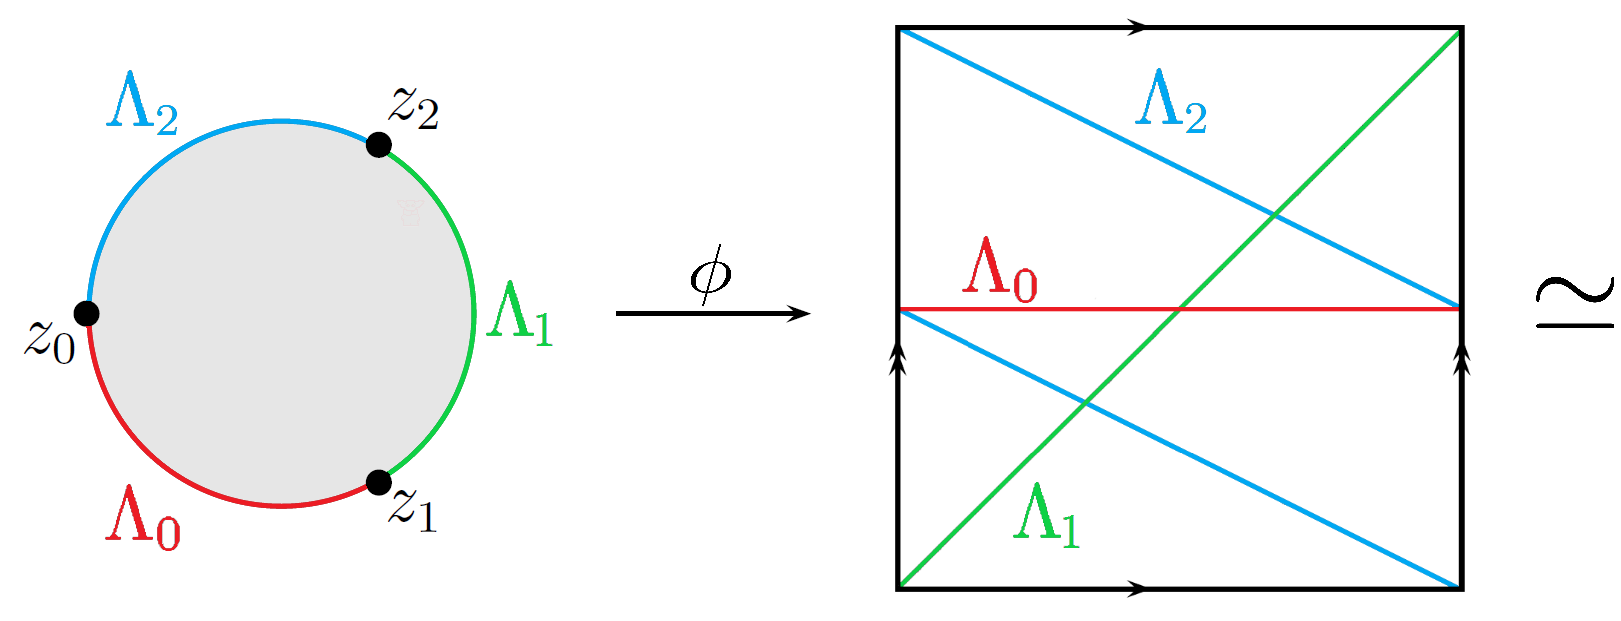
\includegraphics[width=0.6\textwidth]{2toruscompo.png}\quad
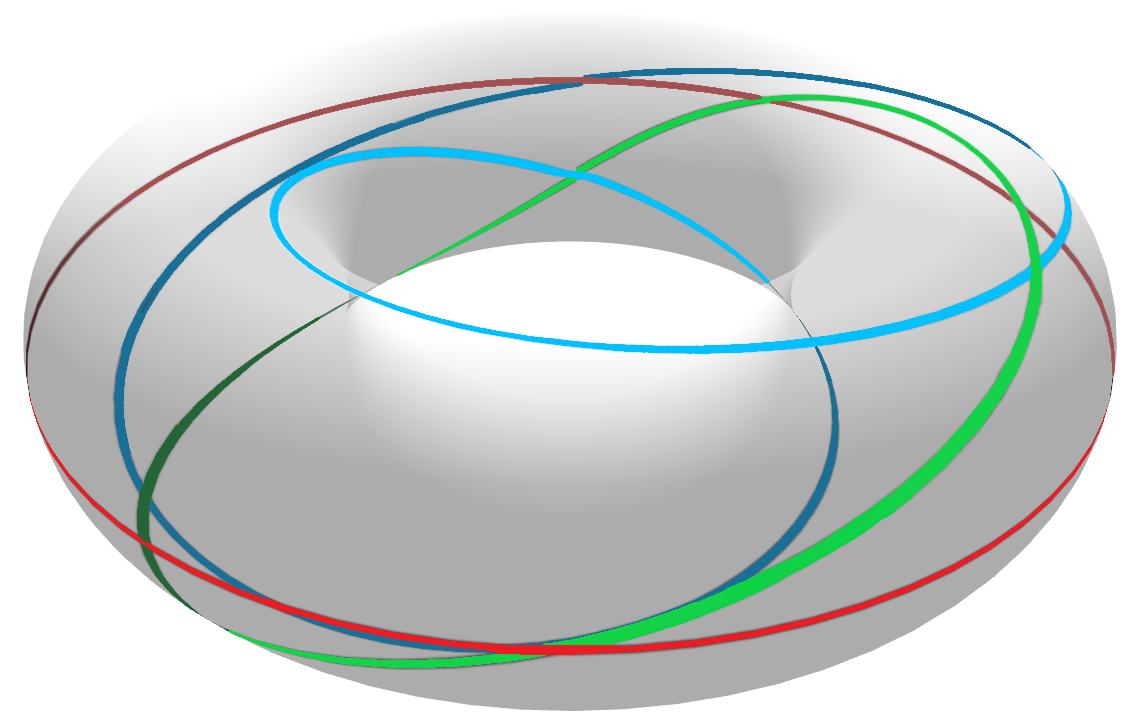
\includegraphics[width=0.35\textwidth]{2torus.png}	
\caption{当拉格朗日子流形彼此不同时，定义复合律所用到的一个可能的映射 $\phi:\mathbb{D}^2\rightarrow E^\rho$。图中特别绘出了 $\mathbb{R}^2$ 模 $\mathbb{Z}^2$ 下的仿射直线 $(t,1/2)$、$(t,t)$ 与 $(t,-t/2+1/2)$，它们分别给出 $\Lambda_0$、$\Lambda_1$ 与 $\Lambda_2$。（原图位置：原 PDF 第 134 页）}
\label{2toruscompo}	
\end{figure}
\vspace*{0.3cm}

% [Tutor Note: 这是全书唯一需要「数圆盘」的地方，也是 $A_\infty$ 范畴的一般定义在此维数下的唯一痕迹。要点：$e^{2\pi i\int\phi^*(\rho dx\wedge dy)}$ 是面积权重——它正是同调镜像对称中把**辛面积** $A$ 与 **B-场** $B$ 合成为复化参数 $\rho=B+iA$ 的物理根源（面积项的相位来自 $B$，模长来自 $A$）。注意 $\phi$ 的边界弧段按**逆时针**依次落入 $\Lambda_0,\Lambda_1,\Lambda_2$，作者用 $z_k\curvearrowright z_{k+1}$ 表示该走向；若把定向约定反过来，则图 \ref{2toruscompo} 中的三角形会取共轭，导致复合律中指数项的符号翻转。]

\noindent 现在我们遇到 \cite{[PZ00]} 最初忽略的主要问题：范畴 $\mathscr{F}^0(E^\rho)$ 是预加性范畴（仅满足定义 \ref{addcat} 的公理 (A1)），却不像一切导出范畴那样是加性范畴（参引理 \ref{D(A)additive}），因为它不含直和，从而不可能构造出同调镜像对称所猜想的任何等价。不过我们注意到下述一般事实。

\begin{Lem}\label{frompreaddtoaddcat}
	设 $\mathsf{C}$ 为预加性范畴，$\underline{\mathsf{C}}$ 为具有如下结构的范畴：
	\begin{itemize}[leftmargin=0.5cm]
		\renewcommand{\labelitemi}{\textendash}

		\item $\textup{obj}(\underline{\mathsf{C}})=\coprod_{k\geq 0}\prod_{l=1}^k\textup{obj}(\mathsf{C})$，于是 $\underline{\mathsf{C}}$ 的对象是 $\mathsf{C}$ 的对象构成的任意长度的有序元组。

		\item 给定 $\underline{X}=(X_1,...,X_k)$ 与 $\underline{Y}=(Y_1,...,Y_l)$（均在 $\textup{obj}(\underline{\mathsf{C}})$ 中，$k,l>0$），令 $\textup{Hom}_{\underline{\mathsf{C}}}(\underline{X},\underline{Y})\coloneqq\prod_{\begin{tiny}1\leq i\leq k, 1\leq j\leq l\end{tiny}}\textup{Hom}_\mathsf{C}(X_i,Y_j)$。随后通过要求零对象 $\underline{0}\in\textup{obj}(\underline{\mathsf{C}})$ 兼具始与终来定义它，即 $\textup{Hom}_{\underline{\mathsf{C}}}(\underline{0},\underline{Y})\coloneqq\{0\}$ 且 $\textup{Hom}_{\underline{\mathsf{C}}}(\underline{X},\underline{0})\coloneqq\{0\}$（若 $\mathsf{C}$ 有零对象 $0_\mathsf{C}$，则任一元组 $(0_\mathsf{C},...,0_\mathsf{C})$ 都同构于 $\underline{0}$）。

		\item 态射的复合律由标准的矩阵乘法给出。
	\end{itemize}
	则 $\underline{\mathsf{C}}$ 是加性范畴，且加性函子 $\mathsf{C}\rightarrow\underline{\mathsf{C}}$（在对象上作用为 $X\mapsto \underline{X}\coloneqq(X)$，即 1-元组）是泛函子（关于「泛」的定义见 \cite[第 III.1 节]{[Har77]}）。
\end{Lem}

这促使我们转而研究由 $\mathscr{F}^0(E^\rho)$ 以此方式诱导的加性范畴，而非 $\mathscr{F}^0(E^\rho)$ 本身。同时，我们开始把模参数 $\rho$ 改记为 $\tau$，以便与将要陈述的同调镜像对称相符。

\begin{Def}\label{FukayaKontsevichcat}
	设 $E^\tau$ 为 2-环面，其分裂封闭导出范畴为 $\mathscr{F}^0(E^\tau)$ $=\mathsf{D}^\pi(\widetilde{\mathscr{F}}(E^\tau))=H^0\big(\Pi(Tw\widetilde{\mathscr{F}}(E^\tau))\big)$。则我们称
	\[
	\mathscr{F\!K}^0(E^\tau)\coloneqq\underline{\mathscr{F}^0(E^\tau)}
	\]
	为 \textbf{Fukaya--Kontsevich 范畴}\index{Fukaya--Kontsevich category}。由引理 \ref{frompreaddtoaddcat} 它是加性范畴，而加性函子 $\mathscr{F}^0(E^\tau)\rightarrow\mathscr{F\!K}^0(E^\tau),\,L\mapsto \underline{L}\coloneqq(L)$ 使我们得以继续在不写下划线的情况下记它的对象与态射。

	对任一 $r\in\mathbb{N}$，令 $p_r:E^{r\tau}\rightarrow E^\tau,\,(x,y)\mapsto(rx,y)$。然后我们定义如下加性函子：
	\begin{itemize}[leftmargin=0.5cm]
		\item $p_{r*}:\mathscr{F\!K}^0(E^{r\tau})\rightarrow \mathscr{F\!K}^0(E^\tau)$，由 $p_{r*}(\Lambda,\alpha,M)\coloneqq (p_r(\Lambda),\alpha',p_{r*}M)$ 给出，其中：$\alpha'\in(k-\frac{1}{2},k+\frac{1}{2}]$ 是满足定义 \ref{F0Erho} 的分次条件的唯一可取之值，而 $k\in\mathbb{Z}$ 由 $\alpha$ 决定（$\alpha$ 必属同一区间）；$p_{r*}M\in\text{GL}(V^{\oplus d})$ 由 $(p_{r*}M)(v_1,...,v_d)\coloneqq(v_2,...,v_d,M(v_1))$ 给出（这里设 $p_r$ 在 $\Lambda$ 上的度数为 $d$）。
		\newline 对任一 $\text{Hom}_{\mathscr{F\!K}^0(E^{r\tau})}(L_0,L_1)$ 中的态射，我们须再次区分 $p_r(\Lambda_0)\neq p_r(\Lambda_1)$、$\Lambda_0=\Lambda_1$ 以及 $\Lambda_0\neq\Lambda_1\,\wedge\,p_r(\Lambda_0)= p_r(\Lambda_1)$ 三种情形，并验证相容性。

		\item $p_r^*:\mathscr{F\!K}^0(E^\tau)\rightarrow\mathscr{F\!K}^0(E^{r\tau})$，取 $p_r^*(\Lambda,\alpha,M)\!\coloneqq\!\bigoplus_{k=1}^n (\Lambda^{(k)},\alpha',(p_r^{(k)})^*M)$，其中：设 $p_r^{-1}(\Lambda)$ 有 $n$ 个连通分支 $\Lambda^{(k)}$，且每个限制 $p_r^{(k)}:\Lambda^{(k)}\rightarrow\Lambda$ 的度数为 $d\coloneqq r/n$；$\alpha'\in(k-\frac{1}{2},k+\frac{1}{2}]$ 仍与 $\alpha$ 同区间；$(p_r^{(k)})^*M=M^d\in\text{GL}(V)$。\footnote{在把局部系统解释为局部常值复向量空间层时，$p_{r*}M$ 表示「给出 $M$ 的那个局部系统之推前」的单值，而 $(p_r^{(k)})^*M$ 表示拉回的单值。} 也正是在这里，「对直和封闭」的必要性显现出来：若 $n>1$，$p_r^*$ 的像并不落在 $\mathscr{F}^0(E^\tau)$ 之中！
		\newline 对态射，我们只需考察拉格朗日子流形相等与不相等两种情形。
	\end{itemize}
\end{Def}

% [Tutor Note: 本节的逻辑主线务必把握：$\mathscr{F}^0$ 只有预加性（Hom-空间是向量空间，但无直和），因此**不可能**与 $\mathsf{D^b}(E_\tau)$（加性）等价——这就是 \cite{[PZ00]} 的漏洞，也是 Kreussler 的贡献所在。引理 \ref{frompreaddtoaddcat} 的「矩阵化」构造 $\underline{\mathsf{C}}$ 是标准的成加性包络（additive envelope）：对象取有限元组、态射取矩阵、复合取矩阵乘法。这样得到的 $\mathscr{F\!K}^0$ 才是可作等价的。另注意 $p_r$ 的推前/拉回在「$n>1$」时确实会跑出原范畴——这正是作者强调「对直和封闭」之处。]

% 译自 arXiv:2306.13589v2 原 tex 第 4190–4389 行
\subsection{一维的同调镜像对称}\label{ch7.3}


我们终于来到椭圆曲线的同调镜像对称的陈述，其恰当的表述见 \cite[定理 4.1]{[Kre00]}。值得指出的是，由两条椭圆曲线构成的镜像对与经典镜像对称的预测相符：对其 Hodge 菱形的分析表明椭圆曲线是自对偶的（见 \cite[例 7.10]{[Imp21]}）。  

\begin{Thm}\label{HMSindim1}
设 $\tau\in\mathbb{C}$ 满足 $\mathfrak{Im}(\tau)>0$。则存在等价
\begin{equation}
	\mathsf{E}_\tau:\mathsf{D^b}(E_\tau)\rightarrow\mathscr{F\!K}^0(E^\tau)
\end{equation}
它与相应的平移函子相容。
\end{Thm}

\begin{proof}(\textit{略述})
我们首先在对象上定义 $\mathsf{E}_\tau$。由注 \ref{indecomposabletorsion}，只需关注不可分解凝聚层 $\mathcal{E}\in\textup{obj}(\mathsf{Coh}(E_\tau;{}_{\mathcal{O}_{E_\tau}}\!\mathsf{Mod}))$；由推论 \ref{indecompocoherentonell}，它们要么是不可分解向量丛，要么是支撑于一点的不可分解挠层。我们按顺序进行。
\begin{itemize}[leftmargin=0.5cm]
	\item 首先设 $\mathcal{E}$ 是形如 $\mathcal{E}=\mathcal{L}_\tau(\varphi)\otimes F_\tau(V,e^N)\in\text{obj}(\mathsf{D^b}(E_\tau))$ 的不可分解向量丛，其中 $\varphi=t_x^*\varphi_0\cdot\varphi_0^{n-1}$ 依命题 \ref{linebundleonell} 取定，$x=a\tau+b\in E_\tau$、$n\in\mathbb{Z}$，而不可分解的 $F_\tau(V,e^N)$ 依定义 \ref{unipotentvectorbundle} 取定。则我们置 
	\[
	\mathsf{E}_\tau(\mathcal{L}_\tau(\varphi)\otimes F_\tau(V,e^N))\coloneqq(\Lambda,\alpha,M)\in\text{obj}(\mathscr{F\!K}^0(E^\tau))\,,
	\]
	其中 $\Lambda\coloneqq(a+t,(n-1)a+nt)/\mathbb{Z}^2$，$\alpha\in(-\frac{1}{2},\frac{1}{2}]$ 是使 $e^{i\pi\alpha}=\frac{1+in}{\sqrt{1+n^2}}$ 的唯一实数，且 $M\coloneqq e^{-2\pi i b\,\text{id}_V + N}$。
	
	\item 现设 $\pi_r:E_{r\tau}\rightarrow E_\tau$ 为同源，且 $\mathcal{E}=\pi_{r*}(\mathcal{L}_{r\tau}(\varphi)\otimes F_{r\tau}(V,e^N))\in\text{obj}(\mathsf{D^b}(E_{\tau}))$——由定理 \ref{AtiyahThm}，这是 $E_\tau$ 上任意不可分解向量丛所取的一般形式。于是，对定义 \ref{FukayaKontsevichcat} 中的 $p_r:E^{r\tau}\rightarrow E^\tau$，我们置
	\[
	\mathsf{E}_\tau(\mathcal{E})\coloneqq p_{r*}\mathsf{E}_{r\tau}(\mathcal{E})=(\Lambda,\alpha,M)\in\text{obj}(\mathscr{F\!K}^0(E^\tau))\,,
	\]
	其中 $\Lambda\coloneqq\big(a+t,(\frac{n}{r}-1)a+\frac{n}{r}t\big)/\mathbb{Z}^2$，$\alpha\in(-\frac{1}{2},\frac{1}{2}]$ 满足 $e^{i\pi\alpha}=\frac{1+in/r}{\sqrt{1+n^2/r^2}}$，而同样 $M\coloneqq e^{-2\pi i b\,\text{id}_V + N}$。
	
	\item 若 $\mathcal{E}=\mathcal{S}(x,V,N)\in\text{obj}(\mathsf{D^b}(E_{\tau}))$ 是支撑于 $x=a\tau+b\in E_\tau$ 的挠层，则我们简单地置
	\[
	\mathsf{E}_\tau(\mathcal{S}(a\tau+b,V,N))\coloneqq((-a,t)/\mathbb{Z}^2,1/2,e^{2\pi i b\,\text{id}_V+N})
	\]
	（从而 $\Lambda$ 是一条经线环路）。   
\end{itemize}
为了在态射上定义 $\mathsf{E}_\tau$，只需建立映射
\[
(\mathsf{E}_\tau)_{\mathcal{E}_1,\mathcal{E}_2}:\text{Hom}_{\mathsf{D^b}(E_\tau)}(\mathcal{E}_1,\mathcal{E}_2[n])\rightarrow\text{Hom}_{\mathscr{F\!K}^0(E^\tau)}(\mathsf{E}_\tau(\mathcal{E}_1),\mathsf{E}_\tau(\mathcal{E}_2)[n])
\]
（对 $n=0,1$，其中 $\mathcal{E}_1,\mathcal{E}_2\in\text{obj}(\mathsf{D^b}(E_\tau))$ 任意）。但由引理 \ref{ellSerreduality} 与「辛」Serre 对偶 \eqref{sympSerreduality}，情形 $n=0$ 实际上已经足够。我们再次分步进行。
\begin{itemize}[leftmargin=0.5cm]
	\item 我们首先处理形如 $\mathcal{E}_i=\mathcal{L}_\tau(\varphi_i)\otimes F_\tau(V_i,e^{N_i})\in\text{obj}(\mathsf{D^b}(E_\tau))$ 的不可分解向量丛，其中 $\varphi_i=t_{x_i}^*\varphi_0\cdot\varphi_0^{n_i-1}$、$x_i=a_i\tau+b_i\in E_\tau$（$i=0,1$），使得 $\mathsf{E}_\tau(\mathcal{E}_i)=(\Lambda_i,\alpha_i,M_i)$ 且 $\Lambda_0\neq\Lambda_1$。由 \cite[命题 2]{[PZ00]}，对任何这样的凝聚层都存在同构 $H^0(\mathcal{L}_\tau(\varphi))\otimes V\cong H^0(\mathcal{L}_\tau(\varphi)\otimes F_\tau(V,e^{N}))$；把它应用于 $\varphi=\varphi_1\varphi_0^{-1}$ 与 $V=\text{Hom}(V_0,V_1)$，我们得到 $\text{Hom}_{\mathsf{D^b}(E_\tau)}(\mathcal{E}_1,\mathcal{E}_2)\cong H^0(\mathcal{L}_\tau(\varphi_1\varphi_0^{-1}))\otimes\text{Hom}(V_0,V_1)$（不妨设 $n_0<n_1$）。 
	\newline 于是，由 $\mathsf{E}_\tau$ 的线性性，只需在形如 $\theta\otimes f\in H^0(\mathcal{L}_\tau(\varphi_1\varphi_0^{-1}))\otimes\text{Hom}(V_0,V_1)$ 的元素上指定它即可，因为 theta 函数构成 $H^0(\mathcal{L}_\tau(\varphi_1\varphi_0^{-1}))$ 的一组基；按命题 \ref{linebundleonell}，我们具体需要给出 $t_{x_{01}}^*\theta[k/(n_1\!-\!n_0),0]((n_1\!-\!n_0)\tau,(n_1\!-\!n_0)z)$ 的指定，其中 $x_{01}=(x_1\!-\!x_0)/(n_1\!-\!n_0)$ 且 $0\leq k<n_1\!-\!n_0$。这一指定是
	\begin{small}\[
		t_{x_{01}}^*\theta\Big[\frac{k}{n_1\!-\!n_0},0\Big]\big((n_1\!-\!n_0)\tau,(n_1\!-\!n_0)z\big)\mapsto e_k\!\coloneqq\!\Big(\frac{a_1\!-\!a_0\!+\!k}{n_1\!-\!n_0},\frac{n_0a_1\!-\!n_1a_0\!+\!n_0k}{n_1\!-\!n_0}\Big)\,,
		\]\end{small}
	\!\!于是这些 $e_k$ 恰是 $\Lambda_0$ 与 $\Lambda_1$ 的交点。拉格朗日子流形重合的情形 $\Lambda_0=\Lambda_1$ 在 \cite{[Kre00]} 中处理。
	
	\item 现在我们想把 $\mathsf{E}_\tau$ 在态射上的定义推广到任意向量丛 $\pi_{r_i*}(\mathcal{E}_i)=\pi_{r_i*}(\mathcal{L}_{r_i\tau}(\varphi_i)\otimes F_{r_i\tau}(V_i,e^{N_i}))\in\text{obj}(\mathsf{D^b}(E_{\tau}))$，其中 $r_0,r_1>0$ 可以相等。其实我们并不推广；感兴趣的读者可在 \cite[定理 4.1]{[Kre00]} 的证明中读到这一步。
	
	\item 若 $\mathcal{E}_0=\mathcal{L}_\tau(\varphi_0)\otimes F_\tau(V_0,e^{N_0})$ 是不可分解向量丛，而 $\mathcal{E}_1=\mathcal{S}(x_1,V_1,N_1)\in\text{obj}(\mathsf{D^b}(E_\tau))$ 是支撑于 $x_1=a_1\tau+b_1\in E_\tau$ 的不可分解挠层，则相应的拉格朗日子流形恰交于一点，由此得到典范同构 $\text{Hom}_{\mathsf{D^b}(E_\tau)}(\mathcal{E}_0,\mathcal{E}_1)\cong\text{Hom}(V_0,V_1)\cong V_0^*\otimes V_1$ 与 $\text{Hom}_{\mathscr{F\!K}^0(E^\tau)}\cong\text{Hom}(V_0,V_1)$。于是 
	\begin{small}
		\begin{align*}
			&(\mathsf{E}_\tau)_{\mathcal{E}_0,\mathcal{E}_1}:V_0^*\otimes V_1\rightarrow V_0^*\otimes V_1\,, \\
			&(f_0,v_1)\mapsto e^{-\pi i(\tau(na_1^2+2a_0a_1)+2(a_1b_0+a_0b_1+na_1b_1))}e^{-(a_0+na_1)f_0\otimes N_1(v_1)+a_1N_0^*(f_0)\otimes v_1}.
		\end{align*}
	\end{small}
	\!\!此外，在更一般的 $\pi_{r_0*}(\mathcal{E}_0)=\pi_{r_0*}(\mathcal{L}_{r_0\tau}(\varphi_0)\otimes F_{r_0\tau}(V_0,e^{N_0}))$ 上，为定义下图中虚线箭头 $(\mathsf{E}_\tau)_{\pi_{r_0*}(\mathcal{E}_0),\mathcal{E}_1}$，需绕道：
	\begin{small}
		\[
		\begin{tikzcd}
			\text{Hom}_{\mathsf{D^b}(E_\tau)}(\pi_{r_0*}(\mathcal{E}_0),\mathcal{E}_1)\arrow[d, "\sim"']\arrow[r, dashed] &  \text{Hom}_{\mathscr{F\!K}^0(E^\tau)}\big(\mathsf{E}_\tau(\pi_{r_0*}(\mathcal{E}_0)),\mathsf{E}_\tau(\mathcal{E}_1)\big) \\ \text{Hom}_{\mathsf{D^b}(E_\tau)}(\mathcal{E}_0,\pi_{r_0}^*(\mathcal{E}_1))\arrow[d, "\mathsf{E}_{r\tau}"'] & \text{Hom}_{\mathscr{F\!K}^0(E^\tau)}\big(p_{r_0*}(\mathsf{E}_\tau(\mathcal{E}_0)),\mathsf{E}_\tau(\mathcal{E}_1)\big)\arrow[u, "\sim"'] \\ \text{Hom}_{\mathscr{F\!K}^0(E^\tau)}\big(\mathsf{E}_\tau(\mathcal{E}_0),\mathsf{E}_\tau(\pi_{r_0}^*(\mathcal{E}_1))\big)\arrow[r, "\sim"'] & \text{Hom}_{\mathscr{F\!K}^0(E^\tau)}\big(\mathsf{E}_\tau(\mathcal{E}_0),p_{r_0}^*(\mathsf{E}_\tau(\mathcal{E}_1))\big)\,,\arrow[u, "\sim"']		
		\end{tikzcd}
		\]
	\end{small}
	\!\!\!其中我们用 \cite[引理 3.4]{[Kre00]} 把源对象的推出换成目标对象的拉回（对 $\pi_{r_0}$ 与 $p_{r_0}$ 都是如此），同时利用了这些态射与 $\mathsf{E}_\tau$ 交换后彼此对应这一事实；映射 $\mathsf{E}_{r\tau}$ 已由上一段可知。我们要指出，$\mathscr{F\!K}^0(E^\tau)$ 的构造在这里是本质性的，因为 $\pi_{r_0}^*(\mathcal{E}_1)$ 一般并不可分解！
	
	\item 最后一种情形是二者皆为不可分解挠层，比如 $\mathcal{E}_i=\mathcal{S}(x_i,V_i,N_i)\in\text{obj}(\mathsf{D^b}(E_\tau))$，支撑于 $x_i=a_i\tau+b_i\in E_\tau$，于是由上述有 $\mathsf{E}_\tau(\mathcal{E}_i)=((-a_i,t)/\mathbb{Z}^2,1/2,e^{2\pi i b_i\,\text{id}_{V_i}+N_i})$。那么：若 $x_0\neq x_1$，则 $\text{Hom}_{\mathsf{D^b}(E_\tau)}(\mathcal{E}_0,\mathcal{E}_1)$、从而 $(\mathsf{E}_\tau)_{\mathcal{E}_0,\mathcal{E}_1}$ 是平凡的；$a_0\neq a_1$ 蕴含 $\Lambda_0\cap\Lambda_1=\emptyset$ 且 $\text{Hom}_{\mathscr{F\!K}^0(E^\tau)}(\mathsf{E}_\tau(\mathcal{E}_0),\mathsf{E}_\tau(\mathcal{E}_1))\cong\{0\}$；$a_0=a_1$ 且 $b_0\neq b_1$ 蕴含 $\Lambda_0=\Lambda_1$ 且 $H^n(\Lambda_0,\mathcal{H}om(M_0,M_1))\cong\{0\}$，这是因为 $M_0$ 与 $M_1$ 没有公共特征值；若 $x_0=x_1$，则 $\text{Hom}_{\mathsf{D^b}(E_\tau)}(\mathcal{E}_0,\mathcal{E}_1)=\text{Hom}_{\mathcal{O}_{E_\tau,x_0}}((V_0,N_0),(V_1,N_1))=\{f\in\text{Hom}(V_0,V_1)\mid f\circ N_0=N_1\circ F,\text{ iff }f\circ M_0=M_1\circ f\}=H^0(\Lambda_0,\mathcal{H}om(M_0,M_1))$。     
\end{itemize}
剩下只需检验 $\mathsf{E}_\tau$ 对于态射的复合表现良好，这将确认它是一个函子。因此，给定任意 $\mathcal{E}_i\in\text{obj}(\mathsf{D^b}(E_\tau))$（$i=0,1,2$），我们必须证明图
\[
\begin{small}
	\begin{tikzcd}
		\text{Hom}(\mathcal{E}_1[k],\mathcal{E}_2[l])\otimes\text{Hom}(\mathcal{E}_0,\mathcal{E}_1[k])\arrow[r, "\circ"]\arrow[d, "\mathsf{E}_\tau\otimes\mathsf{E}_\tau"'] & \text{Hom}(\mathcal{E}_0,\mathcal{E}_2[l])\arrow[d, "\mathsf{E}_\tau"] \\
		\text{Hom}(\mathsf{E}_\tau(\mathcal{E}_1)[k],\mathsf{E}_\tau(\mathcal{E}_2)[l])\otimes\text{Hom}(\mathsf{E}_\tau(\mathcal{E}_0),\mathsf{E}_\tau(\mathcal{E}_1)[k])\arrow[r, "\circ"'] & \text{Hom}(\mathsf{E}_\tau(\mathcal{E}_0),\mathsf{E}_\tau(\mathcal{E}_2)[l])
	\end{tikzcd}
\end{small}
\]
交换，其中 $0\leq k\leq l\leq 1$，而 $\circ$ 表示相应的复合法则。但同样由 Serre 对偶，我们可以只限制到情形 $k=l=0$。我们在此（更加地）语焉不详：
\begin{itemize}[leftmargin=0.5cm]
	\item 若处理的是 $\mathsf{D^b}(E_\tau)$ 中三个不可分解向量丛、其像为三个互不相同的拉格朗日子流形，则与复合的相容性归结为 theta 函数的运算，如 \cite[第 5.2 节]{[PZ00]} 所示。若其中只有两个相等，则把它们的 Hom 空间归结为与单值算子交换的向量空间线性映射的 Hom 空间，而另一个 Hom 空间用 \cite[命题 2]{[PZ00]} 处理。若所有拉格朗日子流形都相等，则可取定义用的 $\varphi$ 映射满足 $\varphi_0=\varphi_1\varphi_2$ 后照此进行。
	
	\item 对由同源的推出给出的、更一般的不可分解向量丛，分析在 \cite[第 5.4 节]{[PZ00]} 中完成。
	
	\item 最后，若这些不可分解凝聚层中至少有一个是挠层，读者可参阅 \cite[第 5.5 节]{[PZ00]}。 
\end{itemize}
上述整套构造已使函子 $\mathsf{E}_\tau$ 是加性的且全忠实。所缺的只是本质满性，补上它便把 $\mathsf{E}_\tau$ 提升为所声称的等价。于是任取 $(\Lambda,\alpha,M)\in\text{obj}(\mathscr{F\!K}^0(E^\tau))$，不妨设其不可分解——这里的意思是 $M$ 不可分解（不是非平凡算子的直和）——那么不妨设它形如 $M=e^{-2\pi i b+N}\in\text{GL}(V)$，其中 $N\in\text{End}(V)$ 循环、$b\in\mathbb{R}$。我们还可以安全地假设 $\alpha\in(-1/2,1/2]$：若 $\alpha=1/2$，则对某个适当的 $-1<a\leq 0$ 有 $(\Lambda,\alpha,M)\cong\mathsf{E}_\tau(\mathcal{S}(-a\tau-b,V,N))$；否则，取互素的 $(r,n)\in\mathbb{N}^2$ 使得 $r+in\in\mathbb{R}e^{i\pi\alpha}$，并设 $a$ 使 $0\leq\frac{ra}{n}<\frac{1}{n}$ 为代表 $\Lambda$ 的直线的最小 $x$ 截距，则有 $(\Lambda,\alpha,M)\cong\mathsf{E}_\tau\big(\pi_{r*}(\mathcal{L}_{r\tau}(t_{ar\tau+b}^*\varphi_0\cdot\varphi_0^{n-1})\otimes F_{r\tau}(V, e^N))\big)$。

因此本质满性得证，1 维的同调镜像对称也随之得证。  
\end{proof}

% [Tutor Note: 这是本节的核心陈述：$\mathsf{E}_\tau$ 把 B-侧的 $\mathsf{D^b}(E_\tau)$ 与 A-侧的 $\mathscr{F\!K}^0(E^\tau)$ 等价起来。务必区分两个记号：$E_\tau=\mathbb{C}/\langle 1,\tau\rangle$ 是 B-侧的复椭圆曲线（$\tau$ 为模参数、$\mathfrak{Im}\tau>0$），而 $E^\tau$ 是 A-侧的辛环面，其复化 Kähler 参数取为 $\tau$（见 U10 的构造）。定理只断言与 $\mathscr{F\!K}^0$（分裂封闭的导出 Fukaya 范畴）的等价，而非与未分裂的 $\mathscr{F}(E^\tau)$。]

我们做到了！（尽管我们略过了相当多的细节。）要求严格的读者请再次参阅 Polishchuk 与 Zaslow 的原始工作——其中讨论了定理 \ref{HMSindim1} 最简单的非平凡版本的一个证明（见 \cite[第 4 节]{[PZ00]}）——以及 Kreussler 的补充论文。特别地，用双方 $A_\infty$-结构表述的复合法则在 \cite{[Pol01]} 中讨论。我们再次指出 \cite{[Por15]} 给出该主题的完整综述，而 \cite{[Rei07]} 深入分析了 $\mathsf{E}_\tau$ 的函子性。

% [Tutor Note: 证明中真正被略去的是「$r>1$（同源推出）情形」与「三个以上对象复合相容性」的验证，作者自己明说 "Actually, we don't"。若要补齐，应查 \cite{[Kre00]}（Kreussler 的定理 4.1 证明）与 \cite{[PZ00]} 第 5.2–5.5 节；本单元只保留了「$r=1$、两两不同拉格朗日」这一最容易图示的情形。]

% [Tutor Note: 原文此处存在若干记号瑕疵，均按原样保留：①「$\text{Hom}_{\mathscr{F\!K}^0(E^\tau)}\cong\text{Hom}(V_0,V_1)$」缺参数；②$\mathcal{E}_0=\mathcal{L}_\tau(\varphi_0)\otimes F_\tau(V_0,e^{N_0})$ 该行中 $n$ 未声明即出现；③最后一条挠层情形里「$f\circ N_0=N_1\circ F$」中的 $F$ 应为 $f$（手写体混淆）；④$(\mathsf{E}_\tau)_{\mathcal{E}_0,\mathcal{E}_1}$ 的公式写成 $e^{-(a_0+na_1)f_0\otimes N_1(v_1)+a_1N_0^*(f_0)\otimes v_1}$，把线性映射放进了指数，疑有脱字。教授引用这些公式时请对照原文或 \cite{[PZ00]}。]

我们再次回顾 \cite[定理 6.4]{[AS09]}：其中基域取为 Novikov 域 $\Lambda_\mathbb{R}$，并具体证明了 2-环面的镜像伙伴是\textit{Tate 椭圆曲线}。


\subsection{二维的同调镜像对称}\label{ch7.4}


如果说椭圆曲线的同调镜像对称看起来已经极不平凡，那么在我们目前的背景下，2 维的情形几乎变得不可捉摸。因此至少可以说，我们的叙述将是粗略的。

首先，让我们弄清 2 维的 Calabi--Yau 流形是什么。就簇而言，我们期待处理的是\textbf{光滑射影曲面}\index{smooth projective surface}。部分论述参见 \cite[第 5.3、21.1 节]{[GHJ03]} 与 \cite[第 10.1 节]{[Huy06]}。

\begin{Def}\label{CY2folds}
$\mathbb{C}$ 上 2 维的 Calabi--Yau 流形或是：
\begin{itemize}[leftmargin=0.5cm]
	\renewcommand{\labelitemi}{\textendash}
	\item \textbf{$K3$ 曲面}\index{k3@$K3$ surface}，是其中唯一作为 Kähler 流形紧且单连通的（因此严格说来，是按定义 \ref{Calabiyauman} 唯一可容许的）；由定义 \ref{Calabiyauvar}，它们是那些典范线丛平凡且 $H^1(X,\mathcal{O}_X)\cong\{0\}$ 的紧复曲面。有些是代数的，即 $\mathbb{C}$ 上 $\mathbb{P}^3$ 中的光滑四次超曲面，例如由零点轨迹 $V(x_0^4+x_1^4+x_2^4+x_3^4)\subset \mathbb{P}^3$ 给出的复代数簇（\textit{Fermat 四次曲面}）；另一些则是阿贝尔曲面的适当商（如 \textit{Kummer 曲面}），或是\textit{椭圆纤维化}、\textit{完全交}。\footnote{虽然并非每个 $K3$ 曲面都是代数的，但代数的那部分仍在所有 $K3$ 曲面的模空间中构成稠密子集。}
	
	\item \textbf{阿贝尔曲面}\index{abelian surface}——即 2 维的\textit{阿贝尔簇}，它们是带有代数群结构的射影代数簇——它们不是单连通的，例如\textit{复} 2 维环面，或等价地实 4-环面 $\mathbb{T}^4$，其中可找到成对椭圆曲线的积。 
	
	\item 文献有时把\textit{Enriques 曲面}与\textit{超椭圆曲面}计入 Calabi--Yau 2-流形。  
\end{itemize}
\end{Def}

由于猜想 \ref{HMSconj} 是专为定义 \ref{Calabiyauman}「严格意义」下的 Calabi--Yau 流形而设的，我们主要关注第一个要点中的对象。

\begin{Rem}
以下是关于 $K3$ 曲面及其近亲的一些相关事实：
\begin{itemize}[leftmargin=0.5cm]
	\item 在 B-侧，与椭圆曲线的情形相反，有界导出范畴无法分辨不同构的 $K3$ 曲面或阿贝尔曲面；换言之，不同的对可以是导出等价的。幸运的是，由 \cite[命题 12.1]{[Huy06]}，这些是 2 维中仅有的例外：若光滑射影簇 $Y$ 的有界导出范畴等价于 $\mathsf{D^b}(X)$，而 $X$ 是既非 $K3$、亦非阿贝尔、也非椭圆的光滑射影曲面，则 $Y\cong X$（作为簇）。要证明这一点，需要关于代数曲面的 Enriques 分类的知识。
	
	\item 任何与 $K3$ 曲面导出等价的光滑射影簇本身也是 $K3$ 曲面（由 \cite[推论 10.2]{[Huy06]}）。事实上，所有 $K3$ 曲面都微分同胚。整体 Torelli 定理（\cite[定理 10.4]{[Huy06]}）进一步断言：两个 $K3$ 曲面同构，当且仅当它们的第二整系数上同调群之间存在 Hodge 等距。
\end{itemize}
\end{Rem}

% [Tutor Note: 这段 Rem 是理解 2 维难点的钥匙：1 维时 $\mathsf{D^b}(E_\tau)$ 决定了 $E_\tau$ 本身，而 2 维时 $K3$ 曲面与阿贝尔曲面存在非平凡的 Fourier--Mukai 导出等价（不同的 $X,Y$ 可以 $\mathsf{D^b}(X)\simeq\mathsf{D^b}(Y)$），因此「B-侧范畴」不再唯一确定几何对象——这正是同调镜像对称在 2 维需要额外数据（如复化 Kähler 类、B-场）的原因。]

Seidel 在 \cite{[Sei13]} 中证明了四次 $K3$ 曲面的一个同调镜像对称版本。我们尝试解释他的结果，所依据的是 \cite[第 8.5 节]{[ABC+09]} 中已经足够简练的概述。 

\begin{Def}\label{Seidelstuff}
设 $\mathbb{C}[[q]]$ 表示 $\mathbb{C}$ 上以形式变量 $q$ 的形式幂级数环（其元素用 $\mathbb{N}_0$ 指标、最终为零的元组来等同）。设
\begin{small}\[
	\mathcal{X}\coloneqq\big\{\big([x_0:x_1:x_2:x_3],q\big)\in\mathbb{P}^3\times\text{Spec}(\mathbb{C}[[q]])\bigm| q\cdot(x_0^4+x_1^4+x_2^4+x_3^4)+x_0x_1x_2x_3=0\big\}
	\]\end{small}
\!\!是一族 Fermat $K3$ 曲面，群
\begin{small}\[
	\Gamma_{16}\!\coloneqq\!\bigg\{(a_0,a_1,a_2,a_3)\!\in\!\mathbb{C}^4\biggm| a_0^4\!=\!a_1^4\!=\!a_2^4\!=\!a_3^4\!=\!\prod_{i=0}^3a_i\!=\!1\bigg\}\Big/\Big\{(a,a,a,a)\!\in\!\mathbb{C}^4\mid a^4\!=\!1\Big\}
	\]\end{small}
\!\!以 $(a_0,a_1,a_2,a_3)\cdot(x_0,x_1,x_2,x_3)\coloneqq(a_0x_0,a_1x_1,a_2x_2,a_3x_3)$ 对角地作用其上，从而得到商 $\widehat{\mathcal{X}}\coloneqq\mathcal{X}/\Gamma_{16}$。

典范映射 $\widehat{\mathcal{X}}\rightarrow\text{Spec}(\mathbb{C}[[q]])$ 的一般纤维 $\widehat{\mathcal{X}}_q$ 是域 $\mathbb{C}((q))\coloneqq\text{Frac}(\mathbb{C}[[q]])$（即 $\mathbb{C}[[q]]$ 的分式域，或形式 Laurent 级数域）上的 $K3$ 曲面，于是我们可以考虑它的有界导出范畴 $\mathsf{D^b}(\widehat{\mathcal{X}}_q)$，更具体地说，考虑 $\mathsf{D^b}(\widehat{\mathcal{X}}_q)\otimes\Lambda_\mathbb{C}$——它由把一切 $\text{Hom}_{\mathsf{D^b}(\widehat{\mathcal{X}}_q)}$-空间与 Novikov 域
\begin{small}\[
	\Lambda_\mathbb{C}\coloneqq\bigg\{\sum_{i\in\mathbb{Z}}a_iq^{\lambda_i}\biggm| a_i\in\mathbb{C}\text{ s.t. }a_i=0\text{ for }i\ll 0,\,\lambda_i\in\mathbb{R} \text{ s.t. }\lambda_i\xrightarrow{i\to\infty}\infty \bigg\}\,.
	\]\end{small}
作张量得到。
\end{Def}

% [Tutor Note: 这里出现了两个「系数域」的转换，容易混淆：①底域从 $\mathbb{C}$ 变为 $\mathbb{C}((q))$（形式 Laurent 级数域）——因为 $\widehat{\mathcal{X}}_q$ 是形式族的一般纤维；②再把 Hom 空间与 Novikov 域 $\Lambda_\mathbb{C}$ 张量，这是 A-侧 Floer 理论的标准做法（Floer 复形以面积为权重取形式幂级数）。第二处的 $\Lambda_\mathbb{C}$ 与 1 维时出现的 $\Lambda_\mathbb{R}$ 只是系数域不同，不是拉格朗日子流形 $\Lambda$。]

\begin{Thm}\textup{（\cite[定理 1.3]{[Sei13]}）}\label{HMSforK3conj}
设 $X\subset\mathbb{P}^3$ 为 $\mathbb{C}$ 上的光滑四次曲面，配以由 $\mathbb{P}^3$ 的 Fubini--Study 度量限制所得的 Kähler 形式，从而视为 Kähler 流形。则存在形式幂级数的自同构 $\psi\in\textup{Aut}(\mathbb{C}[[q]])$ 与三角范畴的等价
\begin{equation}\label{HMSforK3}
	\mathsf{D^\pi}(\mathscr{F}(X))\rightarrow\psi^*(\mathsf{D^b}(\widehat{\mathcal{X}}_q)\otimes\Lambda_\mathbb{C})
\end{equation}
\textup（事实上，两个导出范畴都作为同一范畴的非平凡形变出现。\textup）
\end{Thm}

\begin{proof}(\textit{极为粗略的梗概})
主要策略是对两个集合分别操作，它们（在 \cite[定义 4.15]{[Imp21]} 的意义下）分裂生成 \eqref{HMSforK3} 中的两个范畴。

在 B-侧，Beilinson 定理 \cite[定理 4.72]{[ABC+09]} 断言 $\mathsf{D^b}(\mathbb{P}^3)$ 由 Serre 扭曲的局部自由层构成的集合 $\{\mathcal{O}_{\mathbb{P}^3}(-3),\mathcal{O}_{\mathbb{P}^3}(-2),\mathcal{O}_{\mathbb{P}^3}(-1),\mathcal{O}_{\mathbb{P}^3}\}$ 生成，于是 $\Gamma_{16}$ 的作用产生 $\mathsf{D^b}(\widehat{\mathcal{X}}_q)$ 的 $4\cdot 16=64$ 个分裂生成元。

在 A-侧，$\mathcal{X}$ 在 $\text{Spec}(\mathbb{C}[[q]])$ 上有 4 条奇异纤维，每条含 16 个奇点，共诱导出 64 个拉格朗日球面，可以证明它们分裂生成 $\mathsf{D^\pi}(\mathscr{F}(X))$。

我们提及，迄今为止（或至少在 \cite{[Sei13]} 当时）尚不知道陈述中的映射 $\psi$ 是否与标准镜像映射一致…… 
\end{proof}

% [Tutor Note: 定理中 $\psi^*$ 表示把形式变量 $q$ 沿自同构 $\psi$ 拉回，即「基变换」；它出现是因为 B-侧的量子修正（Gromov--Witten 不变量）依赖于复化 Kähler 参数 $q$ 的选取，而 Seidel 的等价只在某个 $\psi$ 扭变之后才严格成立。64 这个数字的匹配（$4\cdot16$ 与 $4\times16$）是梗概中唯一给出的定量线索。]

\begin{Rem}
定理 \ref{HMSforK3conj} 可以与经典镜像对称的预测相对照，后者断言 $K3$ 曲面的镜像对偶仍是 $K3$ 曲面（见 \cite[例 7.10]{[Imp21]}）。
\end{Rem}

同调镜像对称也被研究于定义 \ref{CY2folds} 中列出的其他「Calabi--Yau 2-流形」。例如，Abouzaid 与 Smith 在 \cite{[AS09]} 中处理 4-环面，Fukaya 在 \cite{[Fuk00]} 中讨论阿贝尔曲面，而 Kontsevich 与 Soibelman 在 \cite{[KS01]} 中关注环面纤维化。 

最后，3 维的同调镜像对称依然（更加）晦暗，正如 Calabi--Yau 3-流形的分类一样，仍是一个未解问题。这当然是弦论学家最着迷的前景，因为 Calabi--Yau 3-流形编码了超弦理论所预言的微观紧致化额外维。最好的直观来自 Strominger、Yau 与 Zaslow 的 \cite{[SYZ96]}，其中通过 T-对偶的物理视角研究镜像对称。（例如可参阅 \cite[第 7.3 节]{[Imp21]} 末尾对 SYZ 猜想的定性描述与一幅漂亮的图。）尽管如此，更高的维数并不总是构成障碍，正如 Sheridan 关于\textit{任意}维复射影空间中 Calabi--Yau 超曲面的同调镜像对称的工作 \cite{[She14]} 所表明的！   

研究仍在继续，但我们最好就此打住。  


\newpage
\thispagestyle{plain}


\clearpage
\section*{展望}
\addcontentsline{toc}{section}{展望}

% [Tutor Note: 本节标题在原 tex 中为 \textbackslash section*\{Outlook\}（带星号），故不会自动进入目录，作者用 \textbackslash addcontentsline 手工补上目录项；译者已把目录项一并改为「展望」，以免目录与正文标题不一致。本节不含数学内容，是作者对全书的方法论反思，可作导读材料阅读。]


在 \cite{[Imp21]} 的结尾段落中，我曾称赞同调镜像对称之美——它能把纯粹数学与理论物理中看似彼此无关的领域纳入同一个屋檐之下。它不过是众多例子之一，说明我们日益增长的数学图景知识正揭示出一个比从前所相信的更为微妙交织的实在。

本工作支持这一看法：它表明同调代数与代数几何这类更「经典」的理论——它们或许不像 A-侧的相当一部分那样严格地服务于 Kontsevich 猜想——能够以出人意料的方式相互作用。然而历史记录告诉我们，许多想法是出于必要性而发展起来的，因而与其诞生的学科内在地纠缠在一起。因此，像这里讨论的这种坚实而独立自足的架构竟能嵌入同调镜像对称这样一头异域怪兽之中，这应当令人惊喜地受到欢迎。这既是一个令人鼓舞的迹象，表明我们走在正确的道路上，也是继续沿此前行的进一步动力——继续前行或许会向我们揭示：仅仅「搬到镜像宇宙」，就拥有解决极其困难问题的力量。

再说一点更浪漫、更私人的话：数学或物理的学生无法不为同调镜像对称这类理论所许诺的统一图景着迷，它撩拨着那种原始的惊奇感——那正是研究工作必不可少的燃料。在这个意义上，我希望读到这些文字的人能因其所呈现的「交响乐」而获得灵感。

但在我变得过于诗意或哲学化之前，就此打住，并向那些读完了我这套完整的同调镜像对称课程的人致敬，以下这幅关于其预测之美的卡通画便是对他们的奖赏。
\vspace*{0.5cm}

% [Tutor Note: 以下为全书最后一张图（原 PDF 第 137 页）。它是作者自制的「自解释」卡通：左侧 A-侧画成辛流形上的拉格朗日子流形，右侧 B-侧画成复流形上的凝聚层，中间以「=」相连——正对应猜想 \ref{HMSconj} 的等价 $\mathsf{D^\pi}(\mathscr{F}(X))\cong\mathsf{D^b}(X^\vee)$。图片文件由主控从原 PDF 无损提取，请勿改动 \includegraphics 行。]

\begin{figure}[htp]
\centering
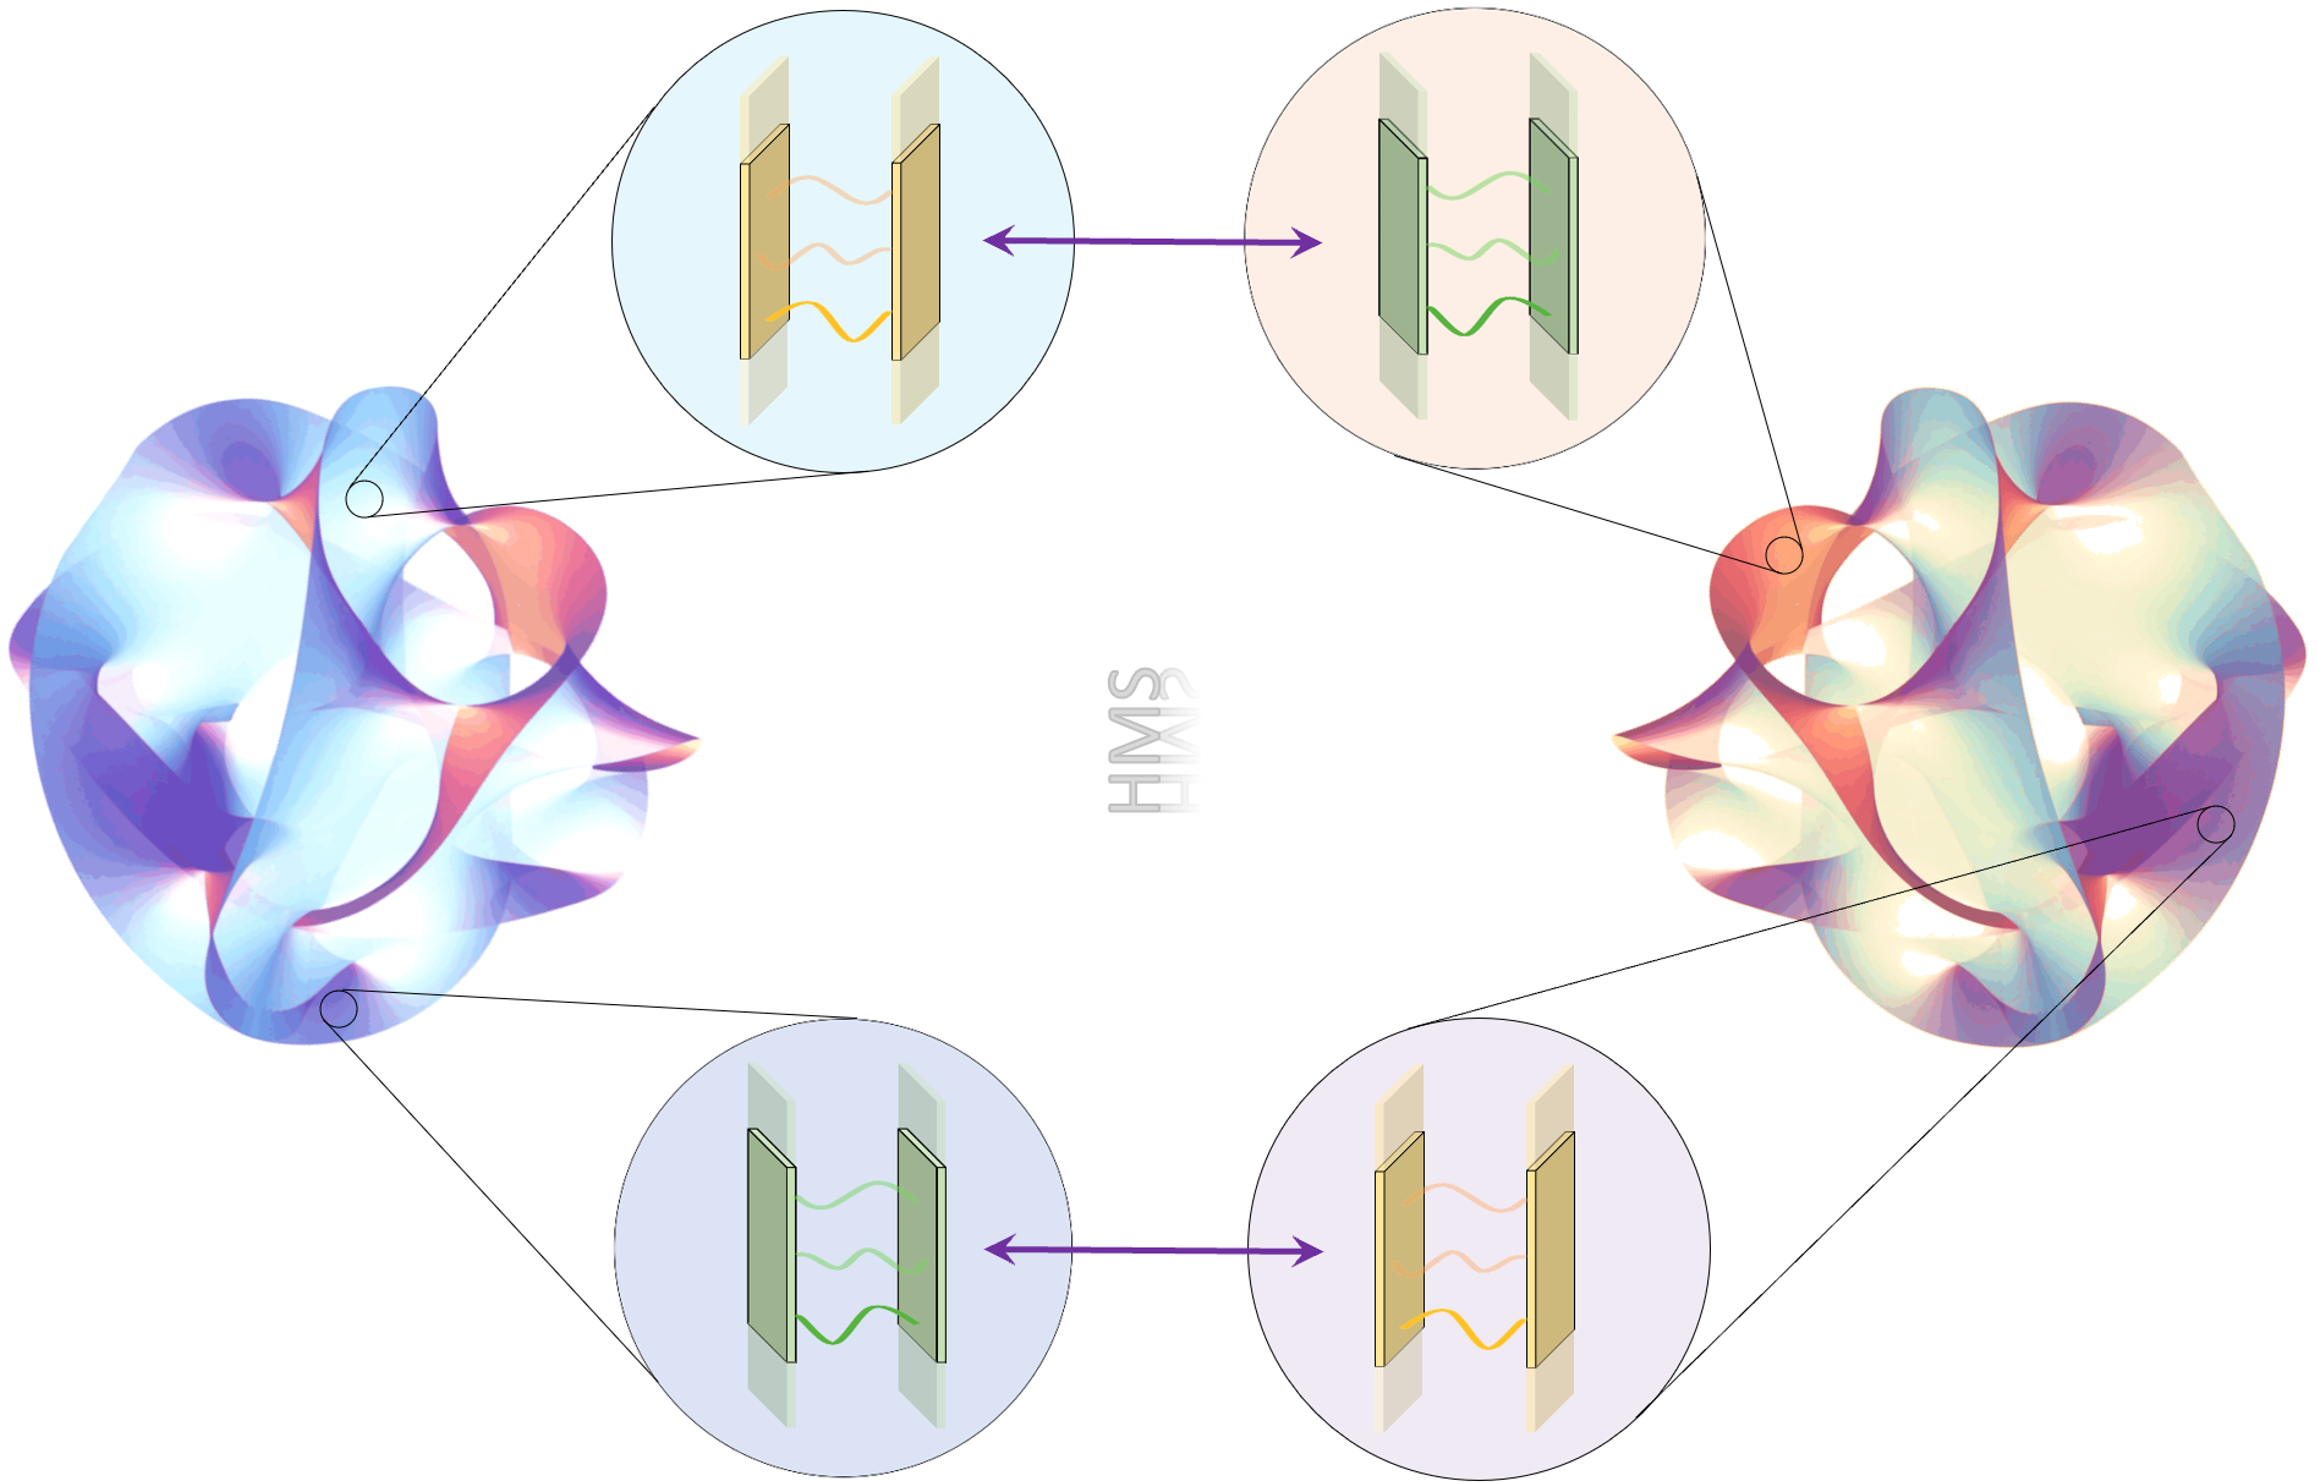
\includegraphics[width=1\textwidth]{HMScartoon.png}
\caption{一幅自解释的同调镜像对称猜想的卡通画。[来源：\begin{footnotesize}\texttt{https://plus.maths.org/content/hidden-dimensions}\end{footnotesize}]（原图位置：原 PDF 第 137 页）}
\end{figure}

\newpage
\thispagestyle{plain}


% ============================================================================
%  appendix_hms.tex —— 附录：英中术语对照表（译者增补，非原文内容）
%  由 work/zh/GUIDE.md 第 7 节词表自动生成；修改词表后重跑 work/mkglossary.py 即可
% ============================================================================

\appendix
\section{英中术语对照表}
\label{app:glossary}

\noindent 本表由译者补入，原文并无此附录。所列为全书反复出现的核心术语，
按主题分组、组内按英文字母序排列，以便对照查阅。数学专名（人名、定理名）与
记号一律保留原文，不作音译。书末的印刷索引为保留字母排序而沿用英文词条，
可与本表对照使用。

\vspace{0.8em}
\noindent\textbf{范畴论 / 同调代数}\par\nobreak
\vspace{0.3em}
{\small
\begin{longtable}{p{0.25\textwidth}p{0.20\textwidth}p{0.25\textwidth}p{0.20\textwidth}}
\toprule
English & 中文 & English & 中文 \\
\midrule
\endhead
category & 范畴 & equalizer / coequalizer & 等化子 / 余等化子\\
set / class & 集合 / 类 & pullback / pushout & 拉回 / 推出\\
object / morphism & 对象 / 态射 & fiber product & 纤维积\\
preadditive category & 预加性范畴 & product / coproduct & 积 / 余积\\
additive category & 加性范畴 & adjoint functor & 伴随函子\\
abelian category & 阿贝尔范畴 & adjunction & 伴随\\
$\mathbb{K}$-linear category & $\mathbb{K}$-线性范畴 & equivalence of categories & 范畴等价\\
functor / bifunctor & 函子 / 双函子 & fully faithful & 全忠实\\
natural transformation & 自然变换 & essentially surjective & 本质满的\\
Hom-set & Hom 集 & full subcategory & 全子范畴\\
zero object / zero morphism & 零对象 / 零态射 & representable functor & 可表函子\\
direct sum (coproduct) & 直和（余积） & Yoneda lemma & Yoneda 引理\\
direct product & 直积 & small / locally small & 小的 / 局部小的\\
biproduct & 双积 & skeleton & 骨架\\
kernel / cokernel & 核 / 余核 & quotient category & 商范畴\\
image / coimage & 像 / 余像 & exact functor & 正合函子\\
monomorphism / epimorphism & 单态射 / 满态射 & left exact / right exact & 左正合 / 右正合\\
isomorphism & 同构 & Freyd–Mitchell embedding theorem & Freyd–Mitchell 嵌入定理\\
subobject / quotient object & 子对象 / 商对象 & Grothendieck category & Grothendieck 范畴\\
universal property & 泛性质 & snake lemma & 蛇引理\\
commutative diagram & 交换图 & five lemma & 五引理\\
limit / colimit & 极限 / 余极限 & diagram chasing & 图追踪\\
\bottomrule
\end{longtable}}

\vspace{0.8em}
\noindent\textbf{复形与导出范畴}\par\nobreak
\vspace{0.3em}
{\small
\begin{longtable}{p{0.25\textwidth}p{0.20\textwidth}p{0.25\textwidth}p{0.20\textwidth}}
\toprule
English & 中文 & English & 中文 \\
\midrule
\endhead
(co)chain complex & （上）链复形 & t-structure & t-结构\\
differential & 微分 & heart of a t-structure & t-结构的核心\\
cohomology / homology & 上同调 / 同调 & truncation & 截断\\
chain map & 链映射 & naive truncation & 朴素截断\\
chain homotopy & 链同伦 & derived functor & 导出函子\\
homotopic & 同伦的 & left / right derived functor & 左 / 右导出函子\\
null-homotopic & 零伦的 & total derived functor & 全导出函子\\
quasi-isomorphism & 拟同构 & injective / projective object & 内射对象 / 投射对象\\
homotopy category & 同伦范畴 & injective / projective resolution & 内射消解 / 投射消解\\
derived category & 导出范畴 & enough injectives & 有足够多的内射对象\\
bounded derived category $\mathsf{D}^b$ & 有界导出范畴 & resolution & 消解\\
split-closed derived category $\mathsf{D}^\pi$ & 分裂封闭导出范畴 & Ext group & Ext 群\\
localization / localize & 局部化 & Tor & Tor\\
multiplicative system & 乘法系统 & spectral sequence & 谱序列\\
calculus of fractions & 分式演算 & short / long exact sequence & 短 / 长正合序列\\
Ore condition & Ore 条件 & hypercohomology & 超上同调\\
saturated & 饱和的 & perfect complex & 完美复形\\
triangulated category & 三角范畴 & homological dimension & 同调维数\\
distinguished triangle & 区分三角形（distinguished triangle） & global dimension & 整体维数\\
exact triangle & 正合三角形 & Verdier quotient & Verdier 商\\
translate / shift / suspension & 平移 / 平移函子 / 悬挂 & Serre subcategory & Serre 子范畴\\
cone / mapping cone & 锥 / 映射锥 & thick subcategory & 厚子范畴\\
octahedral axiom & 八面体公理 & bicomplex / total complex & 双复形 / 全复形\\
cohomological functor & 上同调函子 & Cartan–Eilenberg resolution & Cartan–Eilenberg 消解\\
\bottomrule
\end{longtable}}

\vspace{0.8em}
\noindent\textbf{层论与代数几何}\par\nobreak
\vspace{0.3em}
{\small
\begin{longtable}{p{0.25\textwidth}p{0.20\textwidth}p{0.25\textwidth}p{0.20\textwidth}}
\toprule
English & 中文 & English & 中文 \\
\midrule
\endhead
sheaf / presheaf & 层 / 预层 & of finite type & 有限型的\\
sheafification & 层化 & universally closed & 普遍闭的\\
stalk / germ & 茎 / 芽 & integral / reduced / irreducible & 整的 / 既约的 / 不可约的\\
section / restriction map & 截面 / 限制映射 & quasi-compact / compact & 拟紧的 / 紧的\\
gluing axiom & 粘合公理 & flat / faithfully flat & 平坦的 / 忠实平坦的\\
sheaf of modules / rings & 模层 / 环层 & tensor product & 张量积\\
structure sheaf & 结构层 & vector bundle / line bundle & 向量丛 / 线丛\\
(quasi-)coherent sheaf & （拟）凝聚层 & Picard group & Picard 群\\
locally free sheaf & 局部自由层 & divisor & 因子\\
invertible sheaf & 可逆层 & ample / very ample & 丰富的 / 非常丰富的\\
ringed space / locally ringed space & 环空间 / 局部环空间 & canonical sheaf / canonical bundle & 典范层 / 典范丛\\
global section & 整体截面 & dualizing complex & 对偶复形\\
sheaf cohomology & 层上同调 & Serre duality & Serre 对偶\\
Čech cohomology & Čech 上同调 & Fourier–Mukai transform & Fourier–Mukai 变换\\
scheme & 概形 & Fourier–Mukai kernel & Fourier–Mukai 核\\
variety & 簇（代数簇） & derived equivalence & 导出等价\\
affine / projective variety & 仿射簇 / 射影簇 & Calabi–Yau manifold / variety & Calabi–Yau 流形 / 簇\\
abstract variety & 抽象簇 & Kähler manifold & Kähler 流形\\
quasi-projective & 拟射影的 & holomorphic & 全纯的\\
proper / complete & 固有的 / 完备的 & elliptic curve & 椭圆曲线\\
separated & 分离的 & $K3$ surface & $K3$ 曲面\\
noetherian & 诺特的 & & \\
\bottomrule
\end{longtable}}

\vspace{0.8em}
\noindent\textbf{镜像对称 / 辛几何}\par\nobreak
\vspace{0.3em}
{\small
\begin{longtable}{p{0.25\textwidth}p{0.20\textwidth}p{0.25\textwidth}p{0.20\textwidth}}
\toprule
English & 中文 & English & 中文 \\
\midrule
\endhead
mirror symmetry & 镜像对称 & local system & 局部系统\\
Homological Mirror Symmetry (HMS) & 同调镜像对称 & flat connection & 平坦联络\\
A-side / B-side & A-侧 / B-侧 & curvature & 曲率\\
A-brane / B-brane & A-膜 / B-膜 & holonomy group & 和乐群\\
D-brane & D-膜 & unitary & 酉的\\
Fukaya category & Fukaya 范畴 & B-field & B-场\\
enriched Fukaya category & 富化 Fukaya 范畴 & grading & 分次\\
symplectic manifold & 辛流形 & graded & 分次的\\
symplectic form & 辛形式 & T-duality & T-对偶\\
Lagrangian submanifold & 拉格朗日子流形 & SYZ conjecture & SYZ 猜想\\
special Lagrangian & 特殊拉格朗日 & moduli space & 模空间\\
Maslov index & Maslov 指标 & deformation & 形变\\
Floer cohomology & Floer 上同调 & & \\
\bottomrule
\end{longtable}}

\vspace{0.8em}
\noindent\textbf{结构词}\par\nobreak
\vspace{0.3em}
{\small
\begin{longtable}{p{0.25\textwidth}p{0.20\textwidth}p{0.25\textwidth}p{0.20\textwidth}}
\toprule
English & 中文 & English & 中文 \\
\midrule
\endhead
Introduction & 引言 & Theorem / Lemma / Proposition / Corollary / Conjecture & 定理 / 引理 / 命题 / 推论 / 猜想\\
Abstract & 摘要 & Definition / Example / Remark / Proof & 定义 / 例（例题）/ 注 / 证明\\
Acknowledgments & 致谢 & straightforward / it is obvious that & 直接的 / 显然\\
Key words & 关键词 & the reader may check & 读者可自行验证\\
Chapter / Section / Subsection & 章 / 节 / 小节 & we leave it to the reader & 留待读者自证\\
Part & 部分 & & \\
\bottomrule
\end{longtable}}



% ============================================================================
%  back_hms.tex —— 参考文献与索引
%  对应原 tex 第 4390–4479 行。文献条目按学术惯例保留英文原貌，
%  仅将标题「References」译为「参考文献」。
% ============================================================================

\clearpage
\section*{参考文献}
\addcontentsline{toc}{section}{参考文献}


\begin{thebibliography}{20000000}
\vspace*{0.5cm}

\bibitem[ABC+09]{[ABC+09]} P.S. Aspinwall, T. Bridgeland, A. Craw, M.R. Douglas, M. Gross, A. Kapustin, G.W. Moore, G. Segal, B. Szendröi, P.M.H. Wilson. \textit{Dirichlet branes and mirror symmetry}. Clay Mathematics Monographs, vol. 4, AMS, (2009).
\begin{footnotesize}ISBN\end{footnotesize}: 978-0-8218-3848-8. \begin{footnotesize}URL\end{footnotesize}: \url{http://www.claymath.org/library/monographs/cmim04.pdf}.

\bibitem[AS09]{[AS09]} M. Abouzaid, I. Smith. \textit{Homological mirror symmetry for the four-torus}. Duke Math. J. 152, no. 3 (2010), 373--440, (July 31, 2009). \begin{footnotesize}URL\end{footnotesize}: \url{https://arxiv.org/abs/0903.3065v2}.

\bibitem[Asp04]{[Asp04]} P.S. Aspinwall. \textit{D-branes on Calabi--Yau manifolds}. (March 16, 2004). \begin{footnotesize}URL\end{footnotesize}: \url{https://arxiv.org/abs/hep-th/0403166v1}.

\bibitem[Ati57]{[Ati57]} M.F. Atiyah. \textit{Vector bundles over an elliptic curve}. Proc. London Math. Soc. (3) 7, 414--452, (January 30, 1957). \begin{footnotesize}URL\end{footnotesize}: \url{https://math.berkeley.edu/~nadler/atiyah.classification.pdf}.

\bibitem[BO97]{[BO97]} A. Bondal, D.O. Orlov. \textit{Reconstruction of a variety from the derived category and groups of autoequivalences}. Comp. Math. 125 (2001), no.3, 327--344, (December 24, 1997). \begin{footnotesize}URL\end{footnotesize}: \url{https://arxiv.org/abs/alg-geom/9712029v1}.

\bibitem[Bri98]{[Bri98]} T. Bridgeland. \textit{Equivalences of triangulated categories and Fourier--Mukai
	transforms}. Bull. London Math. Soc. 31 (1999), 25--34, (September 21, 1998).
\begin{footnotesize}URL\end{footnotesize}: \url{https://arxiv.org/abs/math/9809114v2}.

\bibitem[Fuk00]{[Fuk00]} K. Fukaya. \textit{Mirror symmetry of abelian varieties and multi-theta functions}. J. Algebraic Geom. 11, 393--512, (2000). \begin{footnotesize}URL\end{footnotesize}: \url{https://www.math.kyoto-u.ac.jp/~fukaya/abelrev.pdf}.

\bibitem[Gat20]{[Gat20]} A. Gathmann. \textit{Algebraic geometry}. Lecture notes, TU Kaiserslautern, (2019--2020). \begin{footnotesize}URL\end{footnotesize}: \url{https://www.mathematik.uni-kl.de/~gathmann/de/alggeom-2019.php}.

\bibitem[GHJ03]{[GHJ03]} M. Gross, D. Huybrechts, D. Joyce. \textit{Calabi--Yau manifolds and related geometries}. Lectures at a Summer School in Nordfjordeid (June 2001), Springer Universitext, (2003). \begin{footnotesize}ISBN\end{footnotesize}: 978-3-540-44059-8.

\bibitem[GM03]{[GM03]} S.I. Gelfand, Yu.I. Manin. \textit{Methods of homological algebra}. Second edition, Springer Monographs in Mathematics, (2003). \begin{footnotesize}ISBN\end{footnotesize}: 978-3-642-07813-2.

\bibitem[Har77]{[Har77]} R. Hartshorne. \textit{Algebraic Geometry}. Graduate Texts in Mathematics 52, Springer, (1977). \begin{footnotesize}ISBN\end{footnotesize}: 978-1-4757-3849-0.

\bibitem[Hoc19]{[Hoc19]} A. Hochenegger. \textit{Introduction to derived categories of coherent sheaves}. (August 28, 2019). \begin{footnotesize}URL\end{footnotesize}: \url{https://arxiv.org/abs/1901.07305v2}.

\bibitem[HS97]{[HS97]} P.L. Hilton, U. Stammbach. \textit{A course in homological algebra}. Second edition, Graduate Texts in Mathematics 4, Springer, (1997). \begin{footnotesize}ISBN\end{footnotesize}: 978-1-4612-6438-5.

\bibitem[Huy06]{[Huy06]} D. Huybrechts. \textit{Fourier--Mukai transforms in algebraic geometry}. Second edition, Oxford Mathematical Monographs, Oxford University Press, (2006). \begin{footnotesize}ISBN\end{footnotesize}: 978–0–19–929686–6.

\bibitem[Imp21]{[Imp21]} A. Imparato. \textit{Towards homological mirror symmetry}. (August 9, 2021). \begin{footnotesize}URL\end{footnotesize}: \url{https://arxiv.org/abs/2108.03931v1}.

\bibitem[Kon94]{[Kon94]} M. Kontsevich. \textit{Homological algebra of mirror symmetry}. In \textit{Proceedings of the International Congress of Mathematicians}, Birkhäuser, 120--139, (November 30, 1994). \begin{footnotesize}URL\end{footnotesize}: \url{https://arxiv.org/abs/alg-geom/9411018v1}.

\bibitem[Kre00]{[Kre00]} B. Kreussler. \textit{Homological mirror symmetry in dimension one}. (December 4, 2000). \begin{footnotesize}URL\end{footnotesize}: \url{https://arxiv.org/abs/math/0012018v1}.

\bibitem[KS01]{[KS01]} M. Kontsevich, Y. Soibelman. \textit{Homological mirror symmetry and torus fibrations}. (June 4, 2001). \begin{footnotesize}URL\end{footnotesize}: \url{https://arxiv.org/abs/math/0011041v2}.

\bibitem[KS06]{[KS06]} M. Kashiwara, P. Schapira. \textit{Categories and sheaves}. Grundlehren der mathematischen Wissenschaften 332, Springer, (2006). \begin{footnotesize}ISBN\end{footnotesize}: 978-3-540-27949-5.

\bibitem[Mac78]{[Mac78]} S. Mac Lane. \textit{Categories for the working mathematician}. Second Edition, Graduate Texts in Mathematics 5, Springer, (1978). \begin{footnotesize}URL\end{footnotesize}: \url{https://link.springer.com/book/10.1007/978-1-4757-4721-8}. 

\bibitem[May01]{[May01]} J.P. May. \textit{The axioms for triangulated categories}, edited extract from \textit{The additivity of traces in triangulated categories}, Advances in Mathematics 163, 34–-73, (2001). \begin{footnotesize}URL\end{footnotesize}: \url{http://www.math.uchicago.edu/~may/MISC/Triangulate.pdf}.

\bibitem[Mer18]{[Mer18]} W.J. Merry. \textit{Algebraic topology}. Lecture notes, ETH Zürich, (2017--2018).

\bibitem[Orl03]{[Orl03]} D.O. Orlov. \textit{Derived categories of coherent sheaves and equivalences between them}. Russian Math. Surveys, Vol.58 no.3, 511--591, (2003).
\begin{footnotesize}URL\end{footnotesize}: \url{https://homepage.mi-ras.ru/~orlov/papers/Uspekhi2003.pdf}. 

\bibitem[Pol01]{[Pol01]} A. Polishchuk. \textit{$A_\infty$-structures on an elliptic curve}. Commun. Math. Phys. 247 (2004), 527--551, (May 8, 2001). \begin{footnotesize}URL\end{footnotesize}: \url{https://arxiv.org/abs/math/0001048v2}. 

\bibitem[Por15]{[Por15]} A. Port. \textit{An introduction to homological mirror symmetry and the case of elliptic curves}. (January 4, 2015). \begin{footnotesize}URL\end{footnotesize}: \url{https://arxiv.org/abs/1501.00730}.

\bibitem[PZ00]{[PZ00]} A. Polishchuk, E. Zaslow. \textit{Categorical mirror symmetry: the elliptic curve}. Adv. Theor. Math. Phys. 4, 1187--1207, (April 7, 2000). \begin{footnotesize}URL\end{footnotesize}: \url{https://arxiv.org/abs/math/9801119v3}.

\bibitem[Rei07]{[Rei07]} H. Reiter. \textit{On functoriality of homological mirror symmetry of elliptic curves}. Dissertation, Universität Leipzig, (February 15, 2007). \begin{footnotesize}URL\end{footnotesize}: \url{https://www.researchgate.net/publication/255587751_On_Functoriality_of_Homological_Mirror_Symmetry_of_Elliptic_Curves}.

\bibitem[Sei13]{[Sei13]} P. Seidel. \textit{Homological mirror symmetry for the quartic surface}. (August 6, 2013) \begin{footnotesize}URL\end{footnotesize}: \url{https://arxiv.org/abs/math/0310414v4}.

\bibitem[Ser56]{[Ser56]} J.-P. Serre. \textit{Géométrie algébrique et géométrie analytique}. Ann. Inst. Fourier 6, p. 1--42, (1956). \begin{footnotesize}URL\end{footnotesize}: \url{http://www.numdam.org/article/AIF_1956__6__1_0.pdf}.

\bibitem[She14]{[She14]} N. Sheridan. \textit{Homological mirror symmetry for Calabi-Yau hypersurfaces in projective space}. Inventiones Mathematicae, 199 (2015), no. 1, 1--186, (January 13, 2014). \begin{footnotesize}URL\end{footnotesize}: \url{https://arxiv.org/abs/1111.0632}.

\bibitem[SYZ96]{[SYZ96]} A. Strominger, S.-T. Yau, E. Zaslow. \textit{Mirror symmetry is T-duality}. Nucl. Phys. B479, 243--259, (June 14, 1996). \begin{footnotesize}URL\end{footnotesize}: \url{https://arxiv.org/abs/hep-th/9606040v2}.

\bibitem[Vak17]{[Vak17]} R. Vakil. \textit{The rising sea: foundations of algebraic geometry}. Book draft. (November 18, 2017)
\begin{footnotesize}URL\end{footnotesize}: \url{http://math.stanford.edu/~vakil/216blog/FOAGnov1817public.pdf}.

\bibitem[Ver96]{[Ver96]} J.-L. Verdier. \textit{Des catégories dérivées des catégories abéliennes}. Astérisque 239, Société Mathématique de France, (1996). \begin{footnotesize}URL\end{footnotesize}: \url{http://www.numdam.org/issue/AST_1996__239__R1_0.pdf}.

\bibitem[Wei94]{[Wei94]} C. Weibel. \textit{An introduction to homological algebra}. Cambridge Studies in Advanced Mathematics 38, Cambridge University Press, (1994). \begin{footnotesize}URL\end{footnotesize}: \url{https://people.math.rochester.edu/faculty/doug/otherpapers/weibel-hom.pdf}.

\end{thebibliography}

\newpage
\thispagestyle{plain}


\printindex
	


\end{document}
